\documentclass[12pt,oneside,onecolumn,openany,final]{memoir}

\setlength{\paperheight}{10in}
\setlength{\paperwidth}{8in}
\setstocksize{\paperheight}{\paperwidth}

\setlrmarginsandblock{.75in}{.75in}{*}
\setulmarginsandblock{.5in}{.5in}{*}
\checkandfixthelayout

\usepackage[toc,lot,lof]{multitoc}
\usepackage{tocloft}
\usepackage{graphicx}
\graphicspath{{./images/}}
\usepackage{longtable}
\usepackage{mdwlist}
\usepackage{microtype} \DisableLigatures{encoding = *, family = *}
\usepackage{multicol}
\usepackage{textcomp}
\usepackage[normalem]{ulem}
\usepackage{wrapfig}
\usepackage{xtab}
\usepackage{enumerate}
\usepackage{phonetic}
\usepackage{bbding}
\usepackage{linearb}
\usepackage{cypriot}
\usepackage{tipa}
\usepackage{xfrac}
\usepackage{appendix}
\usepackage{array}
\usepackage{multirow}
\usepackage{wasysym}
\usepackage{makeidx} \makeindex
\usepackage[usenames,dvipsnames,table]{xcolor}
\definecolor{tan}{RGB}{255,255,128}
\definecolor{links}{RGB}{200,0,50}
\definecolor{dicePoolColor}{RGB}{0,160,50}
\pagecolor{white}
\usepackage[final]{pdfpages}

%% Font
\usepackage[T1]{fontenc}
\usepackage[bitstream-charter]{mathdesign}
%\usepackage{aurical}

\usepackage[colorlinks=true,linkcolor=blue,urlcolor=links,pdfstartview={XYZ null null 1.00}]{hyperref}
%%%%%%%%%%%%%%%%%%%%%%%%%
%%%% End of Import Section %%%%%%%%%%%
%%%%%%%%%%%%%%%%%%%%%%%%%


%%%%%%%%%%%%%%%%%%%%%%%%%%%%%%%%%%%%%%%%%%%%%%%%%%
%%%%%%%%%%%%%%%%%%%%%%%%%%%%%%%%%%%%%%%%%%%%%%%%%%
%%% Revised Commands
%%%%%%%%%%%%%%%%%%%%%%%%%%%%%%%%%%%%%%%%%%%%%%%%%%
%%%%%%%%%%%%%%%%%%%%%%%%%%%%%%%%%%%%%%%%%%%%%%%%%%
\makeatletter

\renewcommand{\@makechapterhead}[1]{%
\vspace*{0 pt}{
\raggedright \normalfont \fontsize{32}{32} \selectfont \bfseries
\ifnum \value{secnumdepth}>-1
  \if@mainmatter \vspace{-8pt} {\fontsize{20}{20} \selectfont Chapter \thechapter:}\\[8pt]
  \fi%
\fi
\hspace{0.65cm} #1\par\nobreak\vspace{20 pt}
}}

\renewcommand{\paragraph}{%
\@startsection{paragraph}{4}%
{\z@}{1.0ex \@plus 1ex \@minus 0.2ex}{-1em} % wtf is an 'ex' anyways?
{\normalfont\normalsize\bfseries}%
}

\makeatother

%%%%%%%%%%%%%%%%%%%%%%%%%%%%%%%%%%%%%%%%%%%%%%%%%%
%%%%%%%%%%%%%%%%%%%%%%%%%%%%%%%%%%%%%%%%%%%%%%%%%%
%%% New Commands
%%%%%%%%%%%%%%%%%%%%%%%%%%%%%%%%%%%%%%%%%%%%%%%%%%
%%%%%%%%%%%%%%%%%%%%%%%%%%%%%%%%%%%%%%%%%%%%%%%%%%
\newcommand{\tagline}[1]{\vspace{-6pt} \textit{#1} \medskip}
\newcommand{\refwork}[1]{\uline{#1}}
\newcommand{\linkpower}[1]{\hyperref[power:#1]{#1}}
\newcommand{\powerentry}[1]{\paragraph{\textbullet{} #1:}\label{power:#1}\index{#1}}
\newcommand{\skillentry}[1]{\subsection{#1}\label{skill:#1}\index{#1}}
\newcommand{\dicepool}[1]{\textcolor{dicePoolColor}{#1}}

\begin{document}

%%%%%%%%%%%%%%%%%%%%%%%%%%%%%%%%%%%%%%%%%%%%%%%%%%
%%%%%%%%%%%%%%%%%%%%%%%%%%%%%%%%%%%%%%%%%%%%%%%%%%
%%% Title Page
%%%%%%%%%%%%%%%%%%%%%%%%%%%%%%%%%%%%%%%%%%%%%%%%%%
%%%%%%%%%%%%%%%%%%%%%%%%%%%%%%%%%%%%%%%%%%%%%%%%%%
\thispagestyle{empty}
\pagecolor{black}
\begin{center}
{\textsc{\Large}\\[0.95cm]
\color{red}
\fontsize{50}{30} \selectfont \textit{After Sundown}\\[.65cm]
\vfill
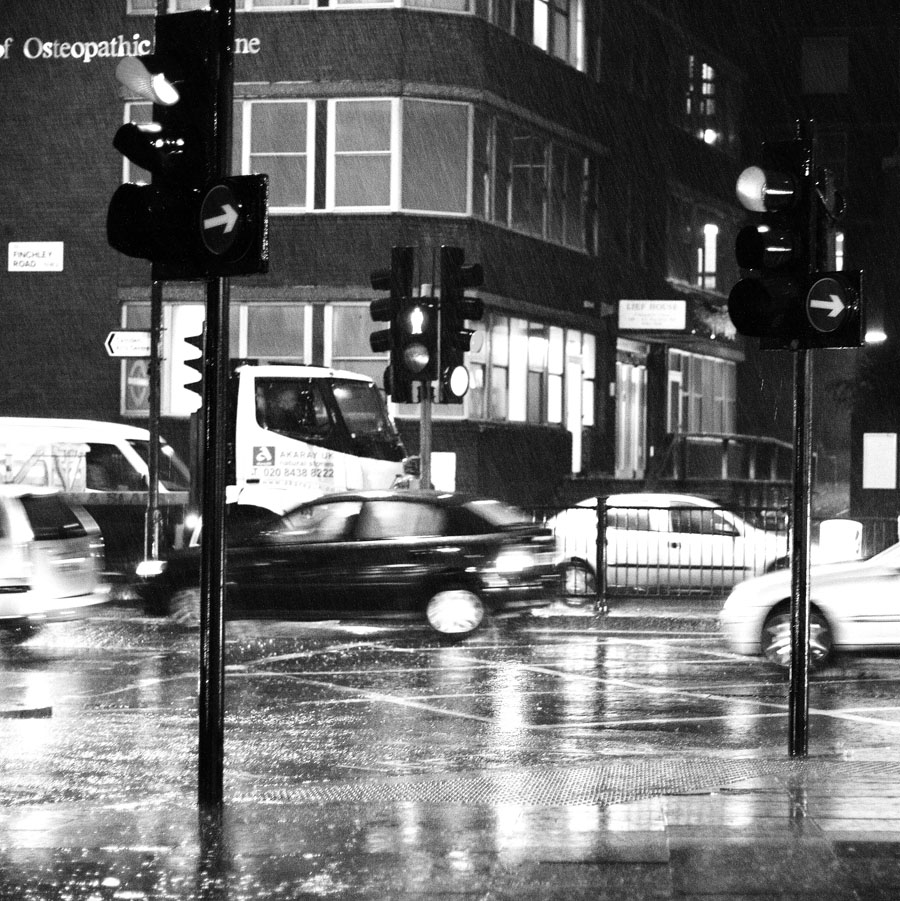
\includegraphics[width=\linewidth]{gagilas_city-blue.jpg}
\fontsize{12}{14} \selectfont
\textit{by Frank Trollman and \href{http://www.tgdmb.com/viewforum.php?f=1}{The Gaming Den}}\\
\today}
\end{center}

%\setcounter{page}{2} %for the version sent to lulu, disable the cover and enable this line

%%%%%%%%%%%%%%%%%%%%%%%%%%%%%%%%%%%%%%%%%%%%%%%%%%
%%%%%%%%%%%%%%%%%%%%%%%%%%%%%%%%%%%%%%%%%%%%%%%%%%
%%% Table of Contents
%%%%%%%%%%%%%%%%%%%%%%%%%%%%%%%%%%%%%%%%%%%%%%%%%%
%%%%%%%%%%%%%%%%%%%%%%%%%%%%%%%%%%%%%%%%%%%%%%%%%%
\pagebreak
\pagecolor{white}
\pagestyle{plain}
\sffamily
\raggedbottom
\setcounter{secnumdepth}{1}
\setcounter{tocdepth}{2}
\renewcommand{\contentsname}{Table of Contents}
\tableofcontents

%%%%%%%%%%%%%%%%%%%%%%%%%%%%%%%%%%%%%%%%%%%%%%%%%%
%%%%%%%%%%%%%%%%%%%%%%%%%%%%%%%%%%%%%%%%%%%%%%%%%%
%%% Main Content
%%%%%%%%%%%%%%%%%%%%%%%%%%%%%%%%%%%%%%%%%%%%%%%%%%
%%%%%%%%%%%%%%%%%%%%%%%%%%%%%%%%%%%%%%%%%%%%%%%%%%

\clearpage{}
%%%%%%%%%%%%%%%%%%%%%%%%%%%%%%%%%%%%%%%%%%%%%%%%%%
%%%%%%%%%%%%%%%%%%%%%%%%%%%%%%%%%%%%%%%%%%%%%%%%%%
\chapter{After Sundown}
%%%%%%%%%%%%%%%%%%%%%%%%%%%%%%%%%%%%%%%%%%%%%%%%%%
%%%%%%%%%%%%%%%%%%%%%%%%%%%%%%%%%%%%%%%%%%%%%%%%%%

\tagline{"I hope you like nightmare worlds!"}

After Sundown is a cooperative storytelling game that tells stories in the realm of horror. Players take on the roles of monsters out of horror movies or the humans who oppose them, while one of the players takes on the role of the MC -- a combination referee, narrator, and roleplayer of last resort for antagonists and minor characters in the story. 

Cooperative storytelling can be done without any products at all, as with collaborative writing or \refwork{Cops and Robbers}. After Sundown provides structure and conflict resolution in the form of an established world and story, as well as with a set of mechanics to determine the results of actions with the help of six sided dice. In this way, players of After Sundown can bypass many of the hangups of both collaborative fiction and Cops and Robbers: most notably the "I shot you/ No you did not" problem. It is hoped that the backstory and established characters of After Sundown will be sufficiently evocative as to give players of protagonists and MCs ample launching points for stories of their own. 

The materials in this book are open content. You can print copies, trade electronic copies with friends, modify the files, or produce derivative work. If you like After Sundown enough, go ahead and "buy" a pdf. But if you'd rather trade it around as a torrent, that is fine too.

%%%%%%%%%%%%%%%%%%%%%%%%%%%%%%%%%%%%%%%%%%%%%%%%%%
\section{After Sundown: An Introduction}
%%%%%%%%%%%%%%%%%%%%%%%%%%%%%%%%%%%%%%%%%%%%%%%%%%
\tagline{To write a story together, everyone must be on the same page.}

One of the primary purposes of a cooperative storytelling \textit{game} is to provide a foundation upon which stories can be told. The other is to provide a framework by which disagreements about how a story should progress can be worked out in an acceptably impartial fashion. 

The setting of After Sundown is a world like our own would be if horror fiction had an element of truth to it. There really are monsters in the night and other worlds full of nightmarish horrors that bleed into the mortal world. But it is also set in a world which is decidedly modern, and that means modern sensibilities. The game's backstory sees history and mythology through a modern interpretation, and adopts horror tropes that resonate with modern audiences. Many horror tropes are timeless -- blood speckled claws in the dark is pretty much always going to be scary -- but many other horror elements are merely puzzling, and are going to be downplayed. The modern audience is not particularly worried about miscegenation or communist invasion, and those elements of old horror fiction are deliberately excluded from their appropriation into After Sundown.

%%%%%%%%%%%%%%%%%%%%%%%%%%%%%%%%%%%%%%%%%%%%%%%%%%
\section{Monster Means Many Things}
%%%%%%%%%%%%%%%%%%%%%%%%%%%%%%%%%%%%%%%%%%%%%%%%%%
\tagline{A story is finite in length.\\
To have anything in it, an infinite number of things must be excluded.}

Ask a dozen people to describe vampires or witches, and you'll get a dozen different answers. And that is a tremendous problem for cooperative storytelling, because everyone is supposedly trying to add to the \textit{same} story. Stories told in After Sundown may have vampires in them, but these are \textit{not} the vampires written about by Stoker or Rice, they are the vampires in the stories told by \textit{your gaming group} set in the realm of horror described in this book. These vampires have an aesthetic that is informed by horror movies, comic books, and both punk and goth subcultures, but they are necessarily different from the monsters described in any particular other work of fiction, and they absolutely do not sparkle.

It is important to note that you can't take everything from myth and legend and cram it into a story. I'm not saying that your story will be completely incoherent, although of course it will be, I'm saying that you are literally incapable of doing that. \refwork{The Vampire Book} is an encyclopedia of just vampire lore from various cultures and it is literally \textit{over nine hundred pages} long. And we're not talking about character backgrounds or rules text or any of the other crap that we know eats up word count like you wouldn't believe. We're talking about just a bare list of facts by mythical origin. And it is still nine hundred pages. And while it is quite comprehensive, there are still vampire facts it does not contain. So it is imperative not only that you acknowledge that you're going to have to cut things down to a manageable amount, but also that you establish specifically what is off limits and what's fair game before you start telling a cooperative story. It is unreasonable to expect that other people sitting down at the table with you think to the same mythic source material when you mention even something as specific as Frankenstein's Monster -- the creature in the book was wicked fast but the Boris Karloff rendition was a lumbering brute.

So we're paring things down. A lot. We don't have, need, or even want a bajillion clans of vampires, or fifteen tribes of werewolves. There \textit{should} be few enough  flavors of things that all the players can remember what the differences between them are. Ideally, people should be able to play whatever supernatural guys they want, sort of like the \refwork{League of Extraordinary Gentlemen}; but in practice you have to put explicit limitations on what is part of the story or things get all weird. Like with Martian invasions and stuff, what was up with that? A story that doesn't have specific exclusions does not truly have any specific inclusions. It's not really a story at all at that point, it's a mess.

The base concept for After Sundown is that you are roleplaying a classic Universal Studios Monster and you engage in narrative driven dramatic role playing of both horror and intrigue. The Universal Horror Films were, if not documentaries, at least "dramatic reenactments" of real events in the shared world you will be telling stories in. The Invisible Man, The Wolfman, The Creature from the Black Lagoon, and of course Dracula were all real people, and the player characters can be creatures like them. And the players in After Sundown can use monster movies old and new for inspiration. But remember that the monsters in every piece of fiction are different, and that while you are telling stories After Sundown that it is the descriptions of monsters \textit{in this book} that break ties. Werewolves can transform voluntarily when the moon isn't full, Golems resist fire, and Vampires do not sparkle. Not because these creatures are like this in every movie, but because that is how they are in the stories told with the After Sundown cooperative storytelling game.

%%%%%%%%%%%%%%%%%%%%%%%%%%%%%%%%%%%%%%%%%%%%%%%%%%
\section{Things You Need To Play}
%%%%%%%%%%%%%%%%%%%%%%%%%%%%%%%%%%%%%%%%%%%%%%%%%%
\tagline{"Assuming flippant things like 'food, water, and shelter' are out of the way."}

After Sundown has one or more players roleplaying as protagonists in the story, and a single player acting as MC. The bare minimum number of players is therefore two, and there is no specific upper limit to the number of players a game of After Sundown can accommodate. It really does seem to work best with between 3 and 6 total players though.

During the game, every single player is going to want some method of keeping track of things. This can be done with pencil and paper, post-it notes, or electronically using laptops or smartphones. Different players prefer note taking and result tallying in different ways, and I won't tell you what format your character has to be kept in. A character sheet has been provided in this book, so if you want to print it out and write on it like we did in the old days, that's fine. Speaking of this book: it is distributed in electronic format, and you'll probably want to reference it (or at least have the capability to reference it) during play. That means that someone will need to bring their laptop or e-reader to the game, or print it out and bring a physical copy to the game instead. You have the right to make as many printed versions of this book as you want for non-commercial purposes, so do what you feel is best.

The actual mechanics of the game require rolling several six sided dice at once to resolve actions. I suggest having at least twelve at the table. But honestly, the more the merrier. Game play is sped up noticeably if each player has their own dice pile in front of them, and some people even like making pre-made piles of different sizes so that they don't have to count dice before rolling. So I wouldn't hazard a number of six sided dice that would serve as a maximum. 

Further, character advancement normally uses draws from a deck of cards (either poker or tarot). Since this is character advancement, it is entirely acceptable to have the card draws happen between sessions or even the beginning of next session. So the game is entirely playable for an entire evening even if no one brought a deck of cards. But \textit{eventually}, you'll want a deck of cards as well. If cards are for whatever reason unavailable, remember that virtually any computer has some sort of solitaire game loaded on it, which will among other things provide an acceptable substitute for any number of card draws.

Since you're going to be telling cooperative stories, you'll want some way to get diagrams across to the other players. This can be done with an erasable mat, or a dry erase board, or a pad of paper in the middle of a table. But it can also be done by sketching things on a computer, provided the screen is large enough for everyone to see.

After Sundown can also be played over the internet by players who each have a computer. You can roll real dice and report the results over internet chat (text or video), or you can use various automatic dice rollers. You'll still want an equal number of players, but they need not be in the same city or even country as one another.

%%%%%%%%%%%%%%%%%%%%%%%%%%%%%%%%%%%%%%%%%%%%%%%%%%
\section{The Role of the MC}
%%%%%%%%%%%%%%%%%%%%%%%%%%%%%%%%%%%%%%%%%%%%%%%%%%
\tagline{"Someone has to have the last word."}

Every player except the MC plays a specific character who is a protagonist in the ensemble fiction that the cooperative storytelling game generates. This allows deeper roleplaying and lends itself to the use of first person pronouns when describing action. However many protagonists there are, there will still be more characters that need to be written into the story, and the actions of these characters are determined by the MC. Note that I say "determined" rather than "played" by, because none of the antagonists, allies, or indifferent background characters are literally the alter ego of the MC. The MC has a very big job in telling the story, but is also the least partisan position, and so it falls to the MC to make snap judgments about what rules apply or what numbers to use for different situations. No rule system can ever be completely comprehensive (there was a comprehensive mathematical proof to that effect by G\"{o}del), and when you run into a situation that the rules \textit{cannot} resolve, the MC should act as an impartial arbitrator.

How much plots for stories are generated by the actions of the protagonists and how much are generated by external events will vary from group to group, but in either case the MC is heavily involved. Even when the other players are producing action and dialog sufficient to drive storytelling, it still falls to the MC to determine what responses are engendered in non player characters (NPCs) or the world around them. Playing the MC is demanding, and some groups rotate the responsibility.

\clearpage{}
%%%%%%%%%%%%%%%%%%%%%%%%%%%%%%%%%%%%%%%%%%%%%%%%%%
%%%%%%%%%%%%%%%%%%%%%%%%%%%%%%%%%%%%%%%%%%%%%%%%%%
\chapter{Terrible Places}
%%%%%%%%%%%%%%%%%%%%%%%%%%%%%%%%%%%%%%%%%%%%%%%%%%
%%%%%%%%%%%%%%%%%%%%%%%%%%%%%%%%%%%%%%%%%%%%%%%%%%
\tagline{"When you say 'the world' do you mean 'Earth', or 'where we are now'?"}

After Sundown takes place in a world with many similarities to our own. A world which has the same countries and cities as the ones we are familiar with, and which is therefore one which you can research by reading about actual places in history and physical space. But it is also secretly full of magic and evil and beasts and slashers from horror fiction. It also has connections to three coterminus magic worlds full of monsters and danger.

It is in short: a game that takes place in the realm of horror rather than the realm of the real. You're playing a cooperative storytelling game, and the genre is horror. It may be action-horror, horror-mystery, horror-comedy, or even horror-romance, but it is always horror.

%%%%%%%%%%%%%%%%%%%%%%%%%%%%%%%%%%%%%%%%%%%%%%%%%%
\section[A Life In Horror]{A Life in Horror: The Good and The Bad}
%%%%%%%%%%%%%%%%%%%%%%%%%%%%%%%%%%%%%%%%%%%%%%%%%%
\tagline{"Interesting fact: The Final Girl trope emerged shortly after young women became a major component of horror movie attendees."}

Life for the common man in After Sundown is actually pretty horrible, and extremely dangerous. Life in After Sundown is life in a horror movie. Or rather, it is a world not unlike Earth would be if all the horror movies were real in different places and at different times. This means that body counts are extremely high, and it is very difficult to get help. This is good news if you happen to be the Bogie Man, but really bad for anyone looking for a life of vaguely normal properties. Here are some important things to remember:

\begin{description}
\item[The Police are no help at all.] Heavily infiltrated by cultists and secret societies, the police in After Sundown are astoundingly ineffective. Sure they will \textit{occasionally} bring down a killer, but the vast majority of crimes go unsolved. Many crimes don't even get investigated, especially if something supernatural is afoot.
\item[Telecommunications are Shoddy.] Sat Phones aren't generally available in the realm of horror. Cellphone coverage cuts out constantly at inopportune moments. Most people still have landlines, but regular telecommunication wires go down frequently and are out for days at a time. The inability to get a call out of a building or town isn't unusual, that kind of thing happens a lot in After Sundown.
\item[People Don't Travel Much.] It's not \textit{weird} for people to not know what goes on in the next town over in After Sundown. Things are just more dangerous, and people keep to themselves more.
\end{description}

Keep this in mind when you're planning your nights in the realm of horror. Life is less connected to other life in the realm of horror and it is \textit{much} easier for dangerous elements to thrive in such an environment.

That being said, it is important to remember that most horror movies begin with people thinking things are pretty normal, and \textit{end} with something of a return to normalcy as well (or do they?) So it's not like Jason is running around the streets murdering people left and right. Indeed, while the death rate from serial and mass murder is large enough in the realm of horror to compete with traffic accidents or opiate abuse, the fact is that you're still more likely to die from cancer. Supernatural creatures remain hidden and the president of the United States is openly a mundane human. A vampire can't just flash their fangs to get free entry to a movie theater, and indeed they could be in a lot of trouble if they flash their fangs in a public space of any kind.

%%%%%%%%%%%%%%%%%%%%%%%%%%%%%%%%%%%%%%%%%%%%%%%%%%
\section{The Four Worlds}
%%%%%%%%%%%%%%%%%%%%%%%%%%%%%%%%%%%%%%%%%%%%%%%%%%
\tagline{"Things are crawling in all over the place these days."}

A very common trope in horror is the inclusion of additional worlds that are full of terror and danger. This is very useful, since of course having an extra world around allows you to fit things into the narrative that would be otherwise very difficult to fit into the Earth. Demon armies, forgotten cities, and strange and deadly plants can be piled to the sky and beyond without otherwise upsetting the world provided that they were never in the world in the first place. Furthermore, the idea that monsters can come in sideways is by itself a wonderfully useful notion for the horror genre, because it severely undermines the concept of safety in a fortress or locked room.

That being said, it is also true that there are a lot of alternate worlds to be had in various stories. Too \textit{many} alternate worlds to be anything vaguely approaching something workable. And so it is that as a compromise we have cut things down to three alternate realities:

\begin{description}
\item[Limbo: The Dark Reflection] The best rendition of the Dark Reflection is probably in \refwork{Silent Hill}. It's a world very much like our own but scoured with demonic powers. Ash falls from the sky like rain and everything looks abandoned or scorched. Demons prowl the Dark Reflection.
\item[Maya: The Dreamlands] Think of a combination of the untamed and deadly dreamworlds of \refwork{Jumanji} or \refwork{Where the Wild Things Are}. This is where dreams and wild things go, but since this is the realm of horror the dreams are often as not inspired by Freddy and the beasts are likely to be the deadly and destructive monsters.
\item[Mictlan: The Gloom] The best rendition of the Gloom is of course in \refwork{Nightwatch}, which even calls the place that. It's a cold and oppressive world where darkness presses insistently upon the light and heat of travelers. Powers of death leak in from every crevice and extinguish fires and the lives of small animals. Blood hungering insects and ghosts scour the Gloom.
\item[The Mortal World] This is the world where most people live. It's just like our world except magic and monsters are real. And it's connected to the three other worlds. It is portrayed in virtually every horror movie because it is the world of every horror movie. Some creatures, particularly the older ones, refer to this world as "Midgard".
\end{description}

Each of these worlds have two levels. One can go to the first level where interaction with the mortal realm is still possible, and one can go to the deeper level where it is not. In short, like in \refwork{Silent Hill} it is possible to straddle the worlds where you can still open and close the door of your house and see what's on the stove but demons from the Dark Reflection can attack you. It's also possible to be all the way in the Dark Reflection, where things are a terrifying hellscape and nothing makes any sense. While in the Shallows of any of the worlds, the celestial realities of Earth appear to hold sway -- the Sun rises and sets while wind and rain appear on schedule. In the Deeps, it becomes apparent that one is quite likely \textit{not on Earth}, as the sky itself betrays one to be on an alien rock.

%%%%%%%%%%%%%%%%%%%%%%%%%
\subsection{Limbo: The Dark Reflection} \index{Limbo}
%%%%%%%%%%%%%%%%%%%%%%%%%
\tagline{"You can go to hell!"\\
"We can't. Not alone\ldots{}"}

A long time ago, some people fucked up really bad and parts of the human world started to fall into the fires of The Dark Reflection. Nobody's quite sure exactly when or what -- some say that it was the cinders of the atomic fires of Oklo, while others say it is the ancient truth contained in the myth of Prometheus and the Scriptural references to Gehenna; some that men merely opened the doorway into the world of ashes; others say that it was men that started the unquenchable fire that begat The Dark Reflection. 

Practically everything found in Limbo was first wrought by humans, and then destroyed by fire. Everywhere in the Dark Reflection there are always remnants of human habitation, and everywhere in the dark reflection, there are always smoke and ashes. Yet it is exceedingly rare to encounter men still living nor open flames still burning. The ground is littered with sooty broken glass: smashed bottles, shattered windows, and  shards of obsidian lie on every surface. The dusty surfaces seem dull, and rarely cast a reflection. When they do, they seem more of a window back to the mortal realm, a cruel reminder of where the onlooker is and where they could be. The sky is perpetually obscured by oppressive smoke and rain falls only infrequently (in many places less than once a year) and it is black with ash when it lands.

The Dark Reflection knows neither day nor night, and languishes eternally in a twilight illumination that comes from between one and four vaguely definable lighter patches in the sky that may well be suns or moons. Limbo is home to the demons: Akuma, Asura, and Ifrit. All of them endeavor merely to survive long enough to escape. Survival is a brutal matter of scavenging amongst the cinders and preying upon the weaker residents. Escape is more difficult, never more than a temporary respite: for each of the dwellers of The Dark Reflection carry the seed of the unquenchable fire within them, and any who escape are doomed to one day start a blaze which will drag another piece of the human world back into The Dark Reflection.

%%%
\subsubsection{Getting to the Dark Reflection}
%%%
\tagline{"Fire doesn't cleanse, it blackens."}

Natural passage in and out of the Dark Reflection is almost always through fires or mirrored surfaces, and it is the latter possibility that gives it its name. Sometimes when something is burned, a rend between the mortal world and the Dark Reflection is left in its place. This is most likely to happen when the burnt thing in question was a source of security such as the wall of a family home or school, or a child's blanket. Once a character has been to the Dark Reflection even once, these portals appear far more commonly in their presence for the rest of their lives. Those who have been to the Dark Reflection often find themselves avoiding mirrors for fear that they will find the profane staring back at them.

Sorcerous means to enter and escape the Dark Reflection can be found in most Infernal paths. Leaving the Dark Reflection is difficult for magical creatures. Whether traveling by sorcery or through a gateway, moving from the Deep to the Shallow or from the Shallow to the Mortal World requires one to make a make a Resistance Test (Social if attempting to traverse a summoning, Mental if attempting to pass through a mirror gate, or Physical if attempting to navigate a burnt rend in space) with a Threshold equal to their own Potency. If returning to a known place, the MC may award a bonus of 1-5 dice to the escape attempt depending upon \textit{how} familiar one is with the location. Summoning rituals and special gate preparations can add additional bonus dice in addition to allowing for an Escape Test at all. The property of being difficult to leave is called "The Gauntlet"\index{Gauntlet}, and it can render the Dark Reflection a near inescapable prison for the very powerful. For example, The King With Three Shadows\index{King with Three Shadows} has a Potency of 10 and suffers from a \textit{name binding} that further raises his escape threshold to 15. The locations of truly epic firestorms have left certain portals that waive these restrictions for supernatural creatures of a Potency equal to or less than their Rating.

%%%
\subsubsection{Things to do in Limbo}
%%%
\tagline{"It's being invaded by the Otherworld. By a world of someone's nightmarish delusions come to life."}

The majority of natives of the Dark Reflection are Goblins and Demons. These beings are generally pretty uncooperative and rarely are on good terms with any of the major Syndicates. The King with Three Shadows\index{King with Three Shadows} has a strong presence in Limbo, and his Syndicate has substantially more territory than any other there. World War II created copies virtually intact of several cities in Limbo, and many of them are used by one or more supernatural groups as bases of operation. The firestorms of Dresden created a dusty and scorched copy of that place in the Dark Reflection which is even now used by members of the Covenant who refused to accept the defeat of the Axis as a base of operation to train a demon army to someday retake the human world. The Rape of Nanking left a level 5 portal to a reflection of the city of Nanjing that is mostly used as a smuggling port by the World Crime League.

Not everything in Limbo is a supernatural creature. There are some real humans there, and they are sad people. Food is scarce in the Dark Reflection, and the nightmarish imagery is usually enough to drive those who fall into Limbo to madness and depravity. Most become demonic pawns. However, demonic pawn or not, a human has no Potency and can pass through the narrowest of portals. All too often, by the time they reach an egress they are already committed to serving dark lords by kidnapping other humans from the mortal world and then \textit{returning} to the land of their torment.

%%%%%%%%%%%%%%%%%%%%%%%%%
\subsection{Maya: The Dreamlands} \index{Maya}
%%%%%%%%%%%%%%%%%%%%%%%%%
\tagline{"Everybody's got to dream, young girl. If you don't dream, ya go crazy."\\
"Go crazy? Don't mind if I do!"}

The Dreamlands are a wild and inhospitable place filled with fetid jungles and monstrous beasts. Overgrown with dreadful, implacable, and nightmarish life in all world correspondences -- even those in the far north and south of the planet (though it still gets wicked cold at extreme latitudes). No one really knows if Maya is a construct of subconscious thought or the manifestation of a distant world that exists independently of our own. What is clear is that Maya is \textit{connected} to the dreams of the frightened and the suffering. The goings on in this world seem somewhat unreal even for those who have traveled to it in the flesh, and the native inhabitants are strange and otherworldly even by the standards set by other supernatural creatures.

The Deep Maya does not even have climactic similarities with its Mortal World correspondences. It boasts floating rocks and sideways waterfalls. And monstrous beasts. And psychic plants. There are few reasons for the sane to want to go to the Deep Maya even though it is wondrous and beautiful in its alien and unforgiving fashion. The weather is pretty similar to that of the Yucatan, with dense cloud cover and hot, driving rain falling almost every day. On those rare times that the night sky is visible, it is clear that the stars above are unfamiliar. The sky boasts no sun or moon, so where precisely the light comes from in the "daytime" is a matter of speculation.

%%%
\subsubsection{Getting to Maya}
%%%
\tagline{"If you die in your dreams, you make me a sandwich."}

Perhaps the easiest way to get to The Dreamlands is to \textit{go to sleep}. While not even a small fraction of dreamers are transported across the barrier, it is nonetheless possible for virtually anyone to make the passage while they are sleeping. A dreamer's physical body remains where it is while the consciousness projects into Maya. If the person dies in the Dreamlands, the body dies as well. If the body dies, the dreamer is lost in Maya indefinitely and becomes a Jalus\index{Spawn!Jalus}. There are places where the barrier between Maya and the sleeping mind is weaker. Generally speaking, places with horrible \textit{personal} murders are more conducive to slipping people across into the nightmare realm. Impersonal deaths, such as natural disasters and battles make the barrier more difficult to cross. Physical gateways, though rare, also exist. They are always circles of something, and one crosses the boundary by entering and then exiting the circle. Circles of mushrooms or trees are fairly common as gateways go, but theoretically it could be a circle of anything. In any case, these gateways only function when the moon is visible. Sorcerous means of entering the Dreamlands are found in Astral Sorceries.

%%%
\subsubsection{Things to do in The Dreamlands}
%%%
\tagline{"We shall build a tower that shall reach to the stars."}

The majority of inhabitants of Maya are neither human nor derived from human stock. Massive monsters stalk the lands and even the plants themselves chitter with an otherworldly malevolence. The Evil Plants in Maya speak to travelers only infrequently. Some can speak telepathically, but they mostly choose not to do so. The Giant Animals generally simply attempt to devour anything they come across. While delicious (if alien) fruit and clearish water are available year round and in great quantity, The Dreamlands have the least expatriot civilization from the Mortal world of all the other worlds.

Not everything in this dimension is from another world however. Sometimes tribes of Jalus congregate together, and for reasons unknown The Marduk Society\index{Marduk Society} all has been growing an Arcanotower in the Brasil Correspondence for some time. They patrol that area and keep it \textit{mostly} clear of Giant Animals, but at least some Evil Plants seem to be allowed free reign to enter the transdimensional compound. 

%%%%%%%%%%%%%%%%%%%%%%%%%
\subsection{Mictlan: The Gloom} \index{Mictlan}
%%%%%%%%%%%%%%%%%%%%%%%%%
\tagline{"Some people believe that when you die there is a wonderful light. As bright as the sun but it doesn't hurt to look into it. All the answers to all the questions you want to know are inside that light. Truth is\ldots{} there is no light. Only darkness."}

The Gloom has been around forever. Some say that it is space itself and the big bang created the human world as a tiny mote within the Gloom, while others say that the Gloom is the force of entropy to which all things shall return in The End. Whatever the case, The Gloom is supernaturally cold and dark.  The ground is bare and everything that lives within The Gloom is hungry all of the time. What plants there are lack essential nutrients and sunlight, and cannot grow without blood. All the insects are parasitic.

There are no visible stars in the Deep Gloom. There is no sun in the morning, and no glittering lights in the night. There \textit{may} be a Moon in the sky, but since it is as fixedly black as anything else in the sky it's a matter of debate. Rain never falls and the seas are deathly still. But water and other things rise up out of the ground at unpredictable times through a process called "welling". If you want light in Mictlan, you need to bring it yourself, and even then the illumination cast by a lamp or flashlight is disappointing, as if the air itself were a voracious shadow.

The Gloom is home to what the unenlightened would call ghosts, wendigos, and zombies. All of them endeavor to draw prey in from the human world where they may drain the blood, life, and warmth from it to feed their insatiable hungers. The true horror is that such victims do not rest in peace, but instead rise driven by the need to recover the blood, life and warmth that was taken from them - in an ever growing cycle of futility. 

%%%
\subsubsection{Getting to Mictlan}
%%%
\tagline{"Have you ever been killed before? I'll be back in a minute."}

Portals to The Gloom are called "wells" and each one is filled with darkness. The most effective portals are holes in the ground filled with shadow and water -- literal wells. However in some cases a well will appear which is \textit{just} a hole filled with water \textit{or} shadow. In addition, pretty much everyone goes to Mictlan just by dying. Upon death, a person becomes a ghost, but in most cases they don't seem to last very long. While some ghosts (especially the ghosts of Luminaries) kick around pretty much indefinitely, this being the realm of horror it seems most likely that ghosts simply unravel and fade into oblivion. The land of the dead is indeed a super depressing place. Sorcerous means of entering The Gloom are found in Orphic magic paths.

While in the Deeper Gloom, all Ghosts are solid, able to be seen and to exert force upon objects. In the Shallow Gloom and to an even greater extent in the mortal world this is not reliably true. So it is that many Ghosts essentially cannot get anything done in the mortal world even if they escape Mictlan through a Well. So while there is no barrier to exit The Gloom as there is for the Dark Reflection, the primary residents mostly do not leave even when they can.

%%%
\subsubsection{Things to do in The Gloom}
%%%
\tagline{"It was their hands that built this city of ours, Father. But where do the hands belong in your scheme?"\\
"In their proper place, the depths."}

Soulless bodies sink into Mictlan fairly regularly, whereupon they are animated by the hungry energies of The Gloom and become wandering zombies. The dusty plains of Mictlan are pretty dangerous for travelers because of this. The Gloom has been around for a long time, and walls erected don't seem to fall down often in the cold stillness of the land of eternal night. Over the millennia many people have found time to erect buildings and even cities. Many of these stand vacant, mute testament to the fact that long ago someone cared enough to build them. However, some are still in use. The Shattered Empire has several such cities, usually corresponding to places where no city or even point of interest stands in the Mortal World. Others are less ambitious, where the Ulmi family have a castle in the Gloom Shadow of Venice.

There does not appear to be any specific fixed limit to how long a Ghost can persist in The Gloom. So even though most last only very short amounts of time, it is entirely possible that any particular historical figure still exists somewhere in Mictlan. Some Ghosts, unhappy with the idea of wandering through a frozen desert for all eternity have taken the time to put up buildings and even societies. The largest such Ancestor City is at about the same place as Beijing.

%%%%%%%%%%%%%%%%%%%%%%%%%
\subsection{Being In Between Worlds}
%%%%%%%%%%%%%%%%%%%%%%%%%
\tagline{You don't have to go home, but you can't stay here.}

In the real world, there is pretty much only one universe you can exist in, and so being in multiple different worlds can be hard to imagine. Here are the states of being one can have:

%%%
\subsubsection{In the Mortal World}
%%%
\hspace{\parindent} This is precisely like being in the universe is for those of us outside the game. A character in the mortal world is safe from attack from things in other worlds, and cannot be physically affected by them. Normal people cannot perceive or touch things in other worlds while they are in the Mortal World. Some disciplines allow characters to perceive, but not touch, things that are in the Shallows of other worlds. So for example, if your character has Necromancy, they can perceive goings-on in the Shallow Gloom, but they are still safe from physically being harmed by creatures or objects there. When a character moves completely from one world to another, they come out in the nearest place that they can fit, which in some cases will be several meters away from their relative location in the original world.

%%%
\subsubsection{In the Shallows}
%%%
\hspace{\parindent} The Shallows of any world are very similar to the Mortal World, and appear to be a compromise of sorts. While a character is in the Shallows, they are essentially in what appears to be a copy of Earth with strange decor, more monsters, and a \textit{lot} less people. The basic lay of the land, including placement and layout of buildings, is almost exactly the same, although there is generally speaking less stuff. 

%%%
\subsubsection{In the Deeps}
%%%
\hspace{\parindent} The Deeps of any world are just completely crazy, and in no way similar to the Mortal World. While there are objects that have been transported or copied from the Mortal World to the Deeps, by and large the Deeps are their own alien wildernesses.

%%%
\subsubsection{Between Worlds}
%%%
\hspace{\parindent} One can occupy both the mortal world and the Shallows of another world, or the Shallows and the Deeps of another world simultaneously. This usually happens while a character is physically in a Bleed (see below), but may also occur during travel from one world to another. Since floors and tables tend to be in the same places in both versions of the world, characters can usually navigate just fine while perceiving and interacting with objects in both worlds simultaneously. The character will appear to be hallucinating to observers from either reality (who aren't also in the Bleed or whatever), because there are things (most especially creatures) that are in only one world and not the other. An effect cannot extend a character into a solid object in the other world, so if a character is standing in empty space in the Shallow Gloom and there's a big pile of sand there in the Mortal World, an event like a convergence or an ability like Shadow Gate would simply fail.

Existence in two worlds is inherently unstable, and is limited in both time and space. If a character moves far enough from their current position or waits for enough time to pass, they \textit{will} end up in one world or the other. And \textit{which} world they end up in is not always predictable (although if the character is in Limbo, they must pass the Gauntlet to end up in more Earthly surroundings). But while a character is between worlds, both prying eyes and bullets from either world can reach them.

%%%
\subsubsection{Bleeds} \index{Bleeds}
%%%
\hspace{\parindent} There are places where the worlds merge, where a character is literally in two worlds because the ground itself is in two worlds. The experience of this is no different than being in just one world at a time, because in such places there is really only one table in the room. And while said table may be in the style of an Earthly table or a table of Limbo, it will still be a single solid object. Where things get weird is at the edges of the Bleed, where a character inside may see two different outsides. Bleeds have a tendency to oscillate between sending those who leave to one world or the other. Sometimes this is very simple (such as opening a door onto either a blighted hellscape or a normal suburban street), and sometimes it's just plain hard to figure out (such as the difference between a foggy forest and a foggy forest that happens to be in Maya). 

%%%%%%%%%%%%%%%%%%%%%%%%%%%%%%%%%%%%%%%%%%%%%%%%%%
\section{Terrible People}
%%%%%%%%%%%%%%%%%%%%%%%%%%%%%%%%%%%%%%%%%%%%%%%%%%
\tagline{Have you gotten a look at the neighbors?}

The realm of horror described in After Sundown is not merely the existence of nightmare worlds from which danger constantly leaks in to disrupt suburban homemaking, it also has people in it. People who are major characters and people who are the victims in slasher flicks. Sometimes, these are the same people.

%%%%%%%%%%%%%%%%%%%%%%%%%%%%%%%%%%%%%%%%%%%%%%%%%%
\section[Extras and Luminaries]{Extras and Luminaries: The People of Horror}
%%%%%%%%%%%%%%%%%%%%%%%%%%%%%%%%%%%%%%%%%%%%%%%%%%
\tagline{"Do not run upstairs! There is no exit upstairs!"}

Remember that in horror movies there are a lot of people who serve no real purpose save to be eaten by the monsters. We call them Extras\index{Extra} even if they happen to get some lines. These people may be strong, or smart, or beautiful, but ultimately they are doomed. If they get bitten by a zombie they will turn into one of the shambling hordes that our heroes must eventually chop through with a chain saw. They will not get cured and will not turn into leaders of the walking dead. Game mechanically, these people have no Edge score. If they turn into a supernatural creature of some kind they will become a \textit{Spawn}\index{Spawn}. These hapless victims will not become the next Dracula, they will always be the horde vampires in \refwork{From Dusk til Dawn}. They will not become Shelly Winters or Sheila, they will join the hordes of deadites and get cleaved through with fire.

On the other side of the coin, there are people in the horror genre who rise to the occasion. Whether they are introduced as bad ass adventurers like Van Helsing or Rick O'Connell, or are "normal people" who rise to the occasion like Meg Penny or Ash, these people have a certain spark of bad assery in them regardless of what they happen to be doing. They are \textit{Luminaries}\index{Luminary}, and they have Edge. If they become Supernaturals they become the real deal. They may turn evil but they will still have lines and character development.

This is why characters will occasionally fight their way through a horde of zombies (who are of course \textit{all} ex-humans) just to try to get a cure for one woman who happens to have been turned into a zombie. It isn't that they've completely lost perspective, it's that the transformation into a monster is a one way trip for absolutely everyone except a reasonably small number of luminaries. You actually can "save" Alice or Sheila if they get transformed into the living dead. There's literally nothing you can do for the rest of the people except shoot them in the face.

%%%%%%%%%%%%%%%%%%%%%%%%%%%%%%%%%%%%%%%%%%%%%%%%%%
\section{The Playable Types}
%%%%%%%%%%%%%%%%%%%%%%%%%%%%%%%%%%%%%%%%%%%%%%%%%%

\hspace{\parindent} The Universal Monsters have a lot of stuff in there which is not really appropriate for emulation. Sure, Lon Chaney is full of awesome and I have no problem watching his movies, but neither the \refwork{Phantom of the Opera} nor the \refwork{Hunchback of Notre Dame} is especially supernatural. They are both just really creepy guys. On the other end of the spectrum, the existence of space aliens really harms the whole eldritch intrigue thing. So while \refwork{This Island Earth} is a good movie and part of the official pantheon, the Metalunans and Zagons are not going to be part of this. At all. 

Which leaves Dracula, Frankenstein's Monster, Gillman, the Mummy, and the Wolfman -- who all appear in the motion picture classic \refwork{The Monster Squad}, and the Evil Wizard, the Invisible Man, and the Mole Man -- who don't. It is of note however that Dracula, Frankenstein's Monster, the Wolfman, and the Invisible Man all appear in the equally mandatory movie \refwork{Abbot and Costello Meet Frankenstein}, and there is of course Evil Wizard and Mummy in the substantially less mandatory \refwork{Abbot and Costello Meet the Mummy}. It seems clear that life would go on without Mole Men; but \textit{what the heck?} We've got Mole Man in After Sundown, we call them Troglodytes.

%%%%%%%%%%%%%%%%%%%%%%%%%
\subsection{Vampires} \index{Vampire}
%%%%%%%%%%%%%%%%%%%%%%%%%
\tagline{An eternity of melancholy and betrayal is, after all, an eternity.}

The Vampire is a rockstar of the living dead. They drink blood, live forever, and look great in black. Vampires are emotionally attenuated individuals who have to consume metaphorical life in the form of actual human blood. They are parasites whose very existence is a powerful metaphor for the consumptive and conflict-torn nature of the world.

\textbf{Exemplars:} Dracula. Did we mention \textit{Dracula}? I mean sure, we can talk about the vampires from \refwork{Blade} or \refwork{Buffy}, and we will even. But all Vampire mythos in the modern world always comes back to Dracula, because he is that awesome. Honorable mention to the beast from Nosferatu, because he is also awesome.

%%%%%%%%%%%%%%%%%%%%%%%%%
\subsection{Animates} \index{Animate}
%%%%%%%%%%%%%%%%%%%%%%%%%
\tagline{Once created, a work has a life of its own.}

An Animate is an artificial person. Created by unwise science, magic, or both, each Animate is a race of one. They have no peers and no possibility of children. Every Animate is created knowing that their entire people dies with them. It is a lonely and frightening existence. The Animate story is classically one that exists to explore the tragedy of dysfunctional human relationships -- whether it be a child scorned by their parents, a lover scorned by the object of their affection, or simply a working person cast aside by those they worked for. The book Frankenstein explores much the same themes as a Bruce Springsteen album. 

\textbf{Exemplars:} Frankenstein's Monster, Rotwang's Robot, Loew's Golem

%%%%%%%%%%%%%%%%%%%%%%%%%
\subsection{Lycanthropes} \index{Lycanthrope}
%%%%%%%%%%%%%%%%%%%%%%%%%
\tagline{Even a man who is pure in heart and says his prayers by night\ldots{}\\
may become a wolf when the wolfbane blooms and the autumn moon is bright}

A Lycanthrope is someone who is cursed to transform into a rampaging beast when the moon is full or they get excited. There is plenty of mythological basis for shapeshifters who are born with the ability to turn into animals or who have attained the magic powers to do so to protect mankind, but they aren't normally figures from \textit{horror} stories, and have no place in horror and are not represented in After Sundown. Being a Lycanthrope means that you are a danger to people you love and the furniture around you. You can unleash the beast to rip things to pieces, but lycanthropy is a \textit{curse} and it is not generally very fun.

\textbf{Exemplars:} John Talbot, Irena Dubrovna, Yuki Sohma

%%%%%%%%%%%%%%%%%%%%%%%%%
\subsection{Witches} \index{Witch}
%%%%%%%%%%%%%%%%%%%%%%%%%
\tagline{Bubble Bubble.}

Witches are people who have learned Magic. In a horror setting, magic is in almost all cases bad. The genre is pretty light on Glinda the Goods and Merlins. Magicians are generally vindictive cackling gypsies, satanic sorcerers, mysterious strangers, and a myriad of other titles both hackneyed and terrifying. They spend a lot more time sacrificing people to gods ancient and evil and a lot less time preparing good children to go to the ball than magicians in other genres.

Magic that humans can use comes from three sources in After Sundown. There is the magic of Death, which is evil. There is Devil magic, which is evil. And finally there is the twisted sorceries of Nightmares, and that's evil as well. It's not that you can't do good as a magician, you totally can. It's just that the magic itself is evil and using it is dangerous even if you are the virtuous Chandu. The horror movies of the 30s didn't distinguish particularly between people from India and China (both were in "The East"), and we hearken to that slightly by leaving all traditions of magic as variations of the basic three. While a character may well be a voodoo death magician or an Aztec or Egyptian death magician, the magical set is all the same. Death magic is death magic whether you call upon bones with Chinese runes or African chants.

An important thing to realize is that The Mummy is actually a Witch.  That's just how they do immortality. Sometimes it's an immortality where you do evil magic and you look like a normal person (see the 1933 \textit{or} 1999 \refwork{The Mummy}) and sometimes you look like a crazy corpse in special bandages (like in \refwork{Bubba Hotep}). It really depends. Either way, if you want to be a leftover from Egypt or Aztlan you are a Witch (or a Vampire of course). However, and this is important, the Mummies from the middle Mummy movies such as \refwork{The Mummy's Ghost} and\ldots{} sigh\ldots{} \refwork{The Mummy's Curse} where the Mummy lurches around and smashes things -- that Mummy is an Animate instead, so pick a schtick and go with it.

\textbf{Exemplars:} Imhotep, Roxor, Hjalmar Poelzig, Chandu

%%%%%%%%%%%%%%%%%%%%%%%%%
\subsection{Transhuman} \index{Transhuman}
%%%%%%%%%%%%%%%%%%%%%%%%%
\tagline{Just a scientific experiment. To do something no other man in the world had done.}

Humans do not, in general, have supernatural powers. However, in the horror genre there are a number of people who experience an event which changes them irrevocably into something different. Something \textit{more}. These people generally go stark raving mad, and in not very long. The certainty that they are no longer human causes them to lose sight of human priorities, human morality. While they have become something more, they are also something \textit{less}.

The transformational event can be scientific or magical. Or a bit of both. A Transhuman always has an "origin story" which is to some degree unique. The Invisible Man took scientific chemicals. Anck Su Namun simply woke up one day and realized that she is the reincarnation of an Egyptian princess. Ayesha stepped into the mystical \textit{flame of life} and stepped out an inhuman thing. Whatever the event was, it was the last thing that he or she did as a human, and the reality of that fact is as destructive to the self as the subsequent  revelations of the magical world and the horrors which inhabit it.

\textbf{Exemplars:} The Invisible Man, Mr. Hyde, Anck Su Namun, Ayesha

%%%%%%%%%%%%%%%%%%%%%%%%%
\subsection{Leviathan} \index{Leviathan}
%%%%%%%%%%%%%%%%%%%%%%%%%
\tagline{His face was fish-like.}

Supposedly in pre-Sumerian times there was a great mother of monsters. Her name was Tiamat. Or Vritra. It's not really that important what her name was, because she was killed by a powerful human sorcerer about 4000 BCE. And most of her monstrous brood is gone as well, but not all of it. Some of them interbred with humans and hid their lineage in the darkest corners of the world. They hid from the world of men for millennia, some lurking in darkness and plotting revenge and others merely living their own lives -- the ancient conflict long forgotten.

But that's not really possible now. Things are modern, and there is nowhere to hide. Those who carry the taint of Tiamat's spawn in their ancestry or are cursed with the taint during their lives are both hunted and feared. They are destructive, and eating their flesh can make you live forever. Of course, eating their flesh makes you like them, and puts you into the same danger. But hey, immortality.

In After Sundown, these creatures often hang out at the edges of society -- places which while nominally explored aren't actually \textit{watched} very carefully. 

\textbf{Exemplars:} Gillman, Mole Man, Robert Olmstead, Moth Man

%%%%%%%%%%%%%%%%%%%%%%%%%%%%%%%%%%%%%%%%%%%%%%%%%%
\section{The Non-Playable Types}
%%%%%%%%%%%%%%%%%%%%%%%%%%%%%%%%%%%%%%%%%%%%%%%%%%

\hspace{\parindent} Not only must we make explicit what appears on the player's side, we also need to decide ahead of time what is around, supernaturally speaking, \textit{in the world}. Many people protest this. If they want to have unicorns show up for a storyline, why shouldn't they, as the MC, just do that? The answer is that in a cooperative storytelling game, the players need some sort of ground state to tell their own back stories and to make plans for future intrigue. Whether or not the \textit{character} knows that such and such a creature exists or such and such a world spanning organization is up to its evil schemes, the \textit{player} needs to at the very least have access to that information. And while it may seem like that would spoil surprises -- and it does sometimes -- in a much more important way it prevents \textit{narrative dissonance}. Narrative dissonance appears in cooperative storytelling games much the way continuity errors appear in horror films. And while it is certainly jarring to watch the part in \refwork{Leprechaun} where they drive off in the second car despite the fact that they had earlier lamented being stranded when the first car wouldn't start -- it is still a movie and thus the plot (such as it is) just keeps rolling along whether you notice the discrepancy or not. In a cooperative storytelling game however, such an event would just crash everything to a halt. The players and the MC would have to sit down and work something out, because they are all imagining the world together and there is no "next scene" until everyone gets their imaginations working together.

%%%%%%%%%%%%%%%%%%%%%%%%%
\subsection{Demons} \index{Demon}
%%%%%%%%%%%%%%%%%%%%%%%%%
\tagline{My God!\\
Not yet, human. Soon\ldots{} very soon I will be.}\

Made entirely of evil magic, the demons are a strange force that seeks to hurt humans and steal souls. Some appear as beautiful humans with or without horns and wings, and others look like the most nightmarish beasts the special effects budget could afford.

\textbf{Examples Include:} Wishmaster, Azazel, Buju, The Lady in Red

%%%%%%%%%%%%%%%%%%%%%%%%%
\subsection{Goblins} \index{Goblins}
%%%%%%%%%%%%%%%%%%%%%%%%%
\tagline{Ha! Ha!}

Fairies in horror movies come from the same ghastly hell dimension that the demons do. These are \textit{not} the shimmering pixies from Neverland, these are the hideous flesh eating goblins from the Goblin Market. They come in small and extra large sizes, and are generally easy to confuse.

\textbf{Examples Include:} The Leprechaun, Rumplestiltskin, Pan, Pyramidhead

%%%%%%%%%%%%%%%%%%%%%%%%%
\subsection{Evil Plants} \index{Evil Plant}
%%%%%%%%%%%%%%%%%%%%%%%%%
\tagline{From now on, I'm shooting my salad }before\textit{ I eat it.}

The evil plants grow out of the ground in weird pods that make the soundtrack want to bust out theremin tracks.  They grow out of humans and often have mind control and other weird powers. These things might actually \textit{be} from Space. But since they don't have a civilization or space ships (that we know of), it's not super important.

\textbf{Examples Include:} Body Snatchers, The Thing, Swamp Thing

%%%%%%%%%%%%%%%%%%%%%%%%%
\subsection{Giant Animals} \index{Giant Animal}
%%%%%%%%%%%%%%%%%%%%%%%%%
\tagline{Rar!}

The wilderness of horror is a dangerous place with a spectacularly large array of things that can kill you. Man eating beasts of tremendous size roam the woods, the lakes, the swamps, and probably the mountains. Being eaten by sharks, crocodiles, tigers, or \textit{whatever} is a severe threat. And yes, these super charged zoo rejects have magic powers sometimes.

\textbf{Examples Include:} Jaws, Joe Young, Boa, Python

%%%%%%%%%%%%%%%%%%%%%%%%%
\subsection{Ghosts} \index{Ghost}
%%%%%%%%%%%%%%%%%%%%%%%%%
\tagline{Boo!}

When humans die and they are \textit{super pissed} about something, they will occasionally linger on after death and become a ghost. Ghosts don't interact properly with physical objects and other people, and in any case are fed only by strong human emotions. So they gradually lose themselves and go batshit crazy, becoming a force that is more and more destructive.
\textbf{Examples Include:} Slimer, Patrick Swayze, The Mist

%%%%%%%%%%%%%%%%%%%%%%%%%
\subsection{Zombies} \index{Zombie}
%%%%%%%%%%%%%%%%%%%%%%%%%
\tagline{Brains!}

Zombies are the result of evil magic, ghastly diseases, or super science which transforms dead bodies into lurching, brain eating monsters. Zombies hunger for the living and have a tendency to rampage constantly. Some zombies are fast, some are slow. Some can figure out doorknobs and others can't. But they all hunger for the living. Zombie spawn can create new zombie spawn just by killing extras, so zombie outbreaks can get really big, really fast.

\textbf{Examples Include:} Shelly Winters, Sheila, Ed

\clearpage{}
%%%%%%%%%%%%%%%%%%%%%%%%%%%%%%%%%%%%%%%%%%%%%%%%%%
%%%%%%%%%%%%%%%%%%%%%%%%%%%%%%%%%%%%%%%%%%%%%%%%%%
\chapter{Running the Game}
%%%%%%%%%%%%%%%%%%%%%%%%%%%%%%%%%%%%%%%%%%%%%%%%%%
%%%%%%%%%%%%%%%%%%%%%%%%%%%%%%%%%%%%%%%%%%%%%%%%%%

\hspace{\parindent} After Sundown is a collaborative storytelling game, where all the players except one take the roles of the protagonists in an ensemble story set in the realm of horror. The odd player out is the MC, who acts as narrator, director, and actor of last resort for all the other characters in the story. The MC has substantial leeway in interpreting how events unfold and is responsible for much of the writing of the backstory. Nevertheless, the story is still \textit{about} the player characters, and no one should forget that.

Player characters will have numbers and abilities written on a character sheet that demonstrate what they are capable of, but in most cases the players themselves will determine what their character actually does. When actions are declared, dice are often rolled to determine the results of the action. But when that is not enough (or would be too tedious as is the case for many minor actions), the MC can deterministically assign results.

Actual stories are told cooperatively, with players bringing up events relevant to their character's backstory and possibilities for the MC to consider weaving into the ongoing description of the world and having real solid first person narrative control over the actions and dialog of their player character. The MC is sometimes said to be "running" the game, because they provide the narrative control on the stage where the protagonists act. 

%%%%%%%%%%%%%%%%%%%%%%%%%%%%%%%%%%%%%%%%%%%%%%%%%%
\section{Basic Dice Mechanics}
%%%%%%%%%%%%%%%%%%%%%%%%%%%%%%%%%%%%%%%%%%%%%%%%%%

\hspace{\parindent} When you perform an action, you roll a pile of d6s called a \index{Dicepool}\textit{dicepool}. Dice which come up as a 5 or 6 are \index{Hits}\textit{hits}. A task will normally require a number of hits to succeed equal to the \index{Threshold}\textit{Threshold}, and any hits gained in addition to that are \index{Net Hits}\textit{Net Hits}. If you get 4 or more net hits, you get a \index{Critical Success}\textit{Critical Success}. If a die roll generates an insufficient number of hits, it is a \index{Failure}\textit{failure}.

\paragraph{Dicepools:} Your dicepool is generally speaking a pile of d6s with dice equal to your character's Attribute + Skill, and circumstantial modifiers increase or decrease the number of dice rolled. A human's attributes and skills go up to 6. A supernatural creature's go up higher than that, both in that their Potency increases their Attribute maximums and that some of their disciplines (magic power groups are called disciplines) further increase their attributes or skills. As such, it is expected that supernatural critters will roll more dice on actions that their powers apply to than normal humans do.

The effects one can expect out of getting a number of Hits are proportionately more awesome as the number of hits increases:

\begin{table}[htb] \rowcolors{1}{white}{tan} \center
\caption[Awesomeness per Hit (Running the Game)]{Awesomeness per Hit}\index{Awesomeness} \hspace{3cm}
\begin{tabular}{c l}
\textbf{Hits:} & \textbf{Awesomeness} \\
\textbf{0:} & Not Awesome. Tying shoes, climbing stairs.\\
\textbf{1:} & Completely Pedestrian. Driving a car, Throwing Darts.\\
\textbf{2:} & Professional. Don't try this at home.\\
\textbf{3:} & Hard. Don't try this at all.\\
\textbf{4:} & Extreme.\\
\textbf{5:} & Crazy Extreme.\\
\textbf{6:} & Super Human. Does not need disclaimers because it is clearly impossible. \\
\end{tabular}
\end{table}

\paragraph{Resistance Tests:} \index{Resistance Tests}Sometimes a character will be allowed to \textit{resist} something being done to them. This is done by rolling dice like normal, save that rather than generating an awesome result, the character is merely reducing the number of hits against them, making whatever is being done to them take less or even no effect. In general, a Physical Resistance Test is simply a Strength roll, a Mental Resistance Test is an Intuition roll, and a Social Resistance Test is a Willpower roll. If a character has an Edge score, it is added to these Resistance tests. When a character is struck with a weapon, they may be called upon to make a Soak\index{Soak Test} roll, which is a special kind of Physical Resistance test. In most cases, if the Resistance Test reduces the number of hits on a test to zero or less, the original attempt has failed.

%%%%%%%%%%%%%%%%%%%%%%%%%%%%%%%%%%%%%%%%%%%%%%%%%%
\section[Basic Attributes]{Basic Attributes: Physical, Mental, and Social}
%%%%%%%%%%%%%%%%%%%%%%%%%%%%%%%%%%%%%%%%%%%%%%%%%%

\hspace{\parindent} Characters in After Sundown have six basic attributes that are divided into Physical, Mental, and Social attributes. These basic attributes range in value between 1 and 6 for normal humans.

\textbf{Physical Attributes}

\hspace{\parindent}\textbf{Strength:} \index{Strength}Strength determines how physically strong \textit{and} tough you are.

\hspace{\parindent}\textbf{Agility:} \index{Agility}Agility is a combination of precision and speed.

\textbf{Mental Attributes}

\hspace{\parindent}\textbf{Intuition:} \index{Intuition}Intuition is a combination of empathic and physical perception.

\hspace{\parindent}\textbf{Logic:} \index{Logic}Logic is a combination of scientific know-how and logical intelligence.

\textbf{Social Attributes}

\hspace{\parindent}\textbf{Willpower:} \index{Willpower}Willpower is a combination of determination and domination.

\hspace{\parindent}\textbf{Charisma:} \index{Charisma}Charisma is one's ability to convince and ingratiate.

The primary purpose of basic attributes is to set the dicepools for actions. A character with a high Agility will have a bunch of extra dice to roll for every skill test that invokes Agility. A character with a high Charisma will have extra dice on every test that uses Charisma, and so on. A character's basic attributes represent a broad aptitude in a wide variety of actions.

%%%%%%%%%%%%%%%%%%%%%%%%%%%%%%%%%%%%%%%%%%%%%%%%%%
\section[Special Attributes]{Special Attributes: Edge, Power, and Potency}
%%%%%%%%%%%%%%%%%%%%%%%%%%%%%%%%%%%%%%%%%%%%%%%%%%

\hspace{\parindent} \textbf{Edge}\index{Edge} is a measure of narrative importance that Luminaries have. You might say it's how much of a protagonist, antagonist, or other sort of main character someone is. All Extras have an Edge of zero. Your Edge stat gives you a number of \textbf{Action Points}\index{Action Points} per chronicle, and also adds to all of your Resistance Tests. Whenever an ability says that the target resists with their Strength or Willpower (or whatever) you can assume that it means "plus Edge" if the target is a Luminary and actually has an Edge stat.

Action Points can be spent in one of several ways:
\begin{itemize*}
\item You can purchase a number of bonus dice on any test equal to your Edge score.
\item You can re-roll all of the failed dice on a test.
\item You can gain an extra Initiative Pass during a combat round.
\item You can avoid a seemingly certain death.
\end{itemize*}

Action Points refresh between chronicles, and you can also regain an Action Point if you do something that puts you closer to achieving your Driving Passion (see Chapter 10).

When you want to spend an Action Point to gain a benefit on a single test, all you really have to do is say that you are doing so. Mark it off and you'll see it again when a new chronicle starts. When spending an Action Point for an extra combat action, you announce that you are doing so at the end of the Initiative Pass that you last acted in. But when you are buying your way out of a deadly situation it is more complicated. At this point you are having fate intervene to save you in a narratively plausible fashion. This will require a negotiation of some kind with the MC to determine what is plausible under the circumstances. Maybe it's the police showing up before the Trolls have the opportunity to put the boot in, maybe it's the floor collapsing and dumping your comatose character into the basement before the flames have an opportunity to burn them to death. It is advisable that a character being saved in such a manner be inconvenienced in some fashion. It's intended as a last ditch save-your-ass moment, not something to be smugly relied upon.

Finally, every two points of Edge a character has also increases the absolute maximum they can raise their skills to during play. While characters start with skill ratings of 6 or less, a character with an Edge of 2 or 3 can eventually raise them to 7, while a character with an Edge of 4 or 5 could raise their skills to 8. A character with an Edge of 6 can potentially get a skill of 9. Six is the maximum Edge for any character (regardless of Potency, as it is a special attribute).

\textbf{Power Reserve}\index{Power Reserve}\index{Power Points} in After Sundown is a parallel attribute similar to Edge. Rather than being spent on any test, Power Points are spent to activate specific supernatural abilities that a character might have. Additionally, you can spend a Power Point to get +2 on a single test to resist magic being used against you. Non-supernatural creatures don't have Power Points at all, and different supernatural creatures refresh their power points in different ways according to their \textit{Power Schedule}\index{Power Schedule}. Characters have a \textbf{maximum} Power at any given time of 10 points plus 3 points per point of Potency. This means that most player characters (who have a Potency of 1) will have their Power Reserve fill up at 13. Mortals and other Potency 0 creatures have a Power Point maximum of 10, but likely have no ability or reason to acquire Power Points.

\medskip

\textit{For example: Genevra is a Vampire with the Quickness ability and the Vigor ability. She can spend 3 Power Points to take extra actions during a scene with her Quickness power. In addition,  She can spend 1 or more Power Points to increase her Strength for a scene with her Vigor power. Because she is a vampire, she can refresh her Power Points by drinking blood from other people.}

\medskip

\textbf{Potency}\index{Potency} When a character's powers increase they may get a special attribute called \textit{Potency}. A character's Potency is added to the \textit{limits} (but not necessarily the actual value) of each of their Physical, Mental, and Social attributes, and every point of Potency increases their maximum Power Reserve by 3. Normal humans and some weak supernatural creatures (such as Mirror Goblins) have a Potency of zero. Starting supernatural creatures of a playable type such as Vampires or Witches have a Potency of 1. This rating gradually rises as the creature ages and grows in eldritch power, and can rise quite abruptly by slaying powerful elders \refwork{Highlander} style or by attuning to powerful artifacts, completing mighty rituals of vast power, or otherwise reaching the kinds of breakpoints in a story in which a monster might become nearly unstoppable. The most powerful named characters in the setting (such as The King with Three Shadows or Echidna) have a Potency of 10, and player characters can expect to have a Potency much, much lower than that.

\medskip

\textit{Genevra is a Vampire with Potency 1. This means that her \textbf{maximum} value for raising her Agility, Willpower, and other attributes is 7. Six maximum for having started as a human, plus her Potency of 1. Her maximum Power Reserve is 13.}

%%%%%%%%%%%%%%%%%%%%%%%%%%%%%%%%%%%%%%%%%%%%%%%%%%
\section{Character Generation}
%%%%%%%%%%%%%%%%%%%%%%%%%%%%%%%%%%%%%%%%%%%%%%%%%%
\tagline{Scene opens on a ringing cellular phone. Camera pans back to reveal\ldots{}}

\index{Character Creation}Characters in After Sundown run the gamut of power. Normal human extras are slaughtered in groups by monsters run amok in the fine tradition of slasher movies the world over.  And yet even those monsters live in terror of even larger monsters from the ancient past. It can best be thought of in terms of regular horror movies going on simultaneously with the events from \refwork{Hellboy} or \refwork{Queen of the Damned}. The Characters are created at a point just before the story starts. And thus, the point where the characters begin is dependent upon what kind of story is being told:

\begin{description}
\item[The Origin Story:] \index{Origin Story}The characters begin with little or no knowledge of the supernatural as human Luminaries. Over the course of the story they discover magical powers within themselves, attain magical powers, or simply come into conflict with supernatural agents.

\item[The In Media Res Adventure:] \index{In Media Res}The characters begin having already been supernatural creatures for some time. They have come to terms with what they are, they have made social connections amongst other supernatural creatures, and they are already members of supernatural organizations.

\item[The Power Fantasy:] \index{Power Fantasy}The characters begin already powerful within the context of supernatural society. Each character is a thing to be feared, whose name is uttered in whispered tones by creatures who themselves inspire fear in mortal hearts.
\end{description}

Regardless of what kind of story is being told, remember that it is going to be an ensemble cast with each player's character being one of the story driving protagonists. Each character thus should have interests and goals that drive the plot forward, not just passive interests or reactive interests. It's fine for a character to be a doctor or a police officer, but they can't just be a passive observer waiting for people to get sick or cars to be reported stolen. A character worth playing thus needs to have a goal that they can work towards when there \textit{isn't} a fire to be put out. It's fine to play a character who can heal others, but the character \textit{needs} a hook that can get them motivated to pursue goals and advance the plot when there isn't anyone injured in their presence.

%%%%%%%%%%%%%%%%%%%%%%%%%
\subsection[Origin Story]{Characters for an Origin Story}
%%%%%%%%%%%%%%%%%%%%%%%%%
\tagline{Don't be silly, there's no such thing as vampires.}

In an Origin Story\index{Origin Story}, the characters are, or at least \textit{believe themselves} to be mortal humans. As such, the player creates their character as if they were a mortal human Luminary. Generally over the course of the story, the player characters will be embraced by vampires, mauled by werewolves, or even discover that their memories of growing up in Indiana are digital imprints and they've been a robot the entire time. But becoming cursed with magic powers or discovering that they have had them all along is something that doesn't happen until after character generation. This makes characters who are substantially better than normal humans and makes sure that they have a diverse set of competencies. They \textit{are} the Protagonists, after all.

\begin{description}
\item[Attributes]
All of a character's attributes start at 1. The player then prioritizes their Physical, Mental, and Social attributes, distributing 1 point to one pair, 3 points to another pair and 5 points to the last pair. Then they get 2 additional points that they can place anywhere they want. An individual attribute cannot be higher than 6 on character creation.
Luminaries begin the game with an Edge of 3.

\item[Active Skills]
A character's Active Skills start at zero. The player then prioritizes their Physical, Social, and Technical skills, distributing 11 points to one set, 16 points to the next set, and 21 points to the last set. Then they get 6 points they can place anywhere they want. An individual skill cannot be higher than 6 on character creation. The character then chooses three skill specializations. Remember that they also gain a specialization for each Technical skill they have trained.

\item[Backgrounds]
A character starts with 27 points of Backgrounds. No Background can start higher than rating 6. An important thing to note is that a character in an Origin Story has a job, some social networks and maybe a family. They almost certainly \textit{don't} have Backgrounds like "Makhzen Society" or "Black Spot Ethos." 

\item[Resources]
The player chooses one 3-point Resource, one 2-point Resource, and one 1-point Resource. At the MC's discretion, a player may be able to buy more Resources with Obligations. Mortal humans are not normally able to take Destiny or Secrets.

\item[Motivations]
Human characters do not normally have Master Passions. However, they still do have Driving Passions and Ethical Taboos. So the player should define some for their character. The player should really think about what their character wants, and what their character is willing to do to get what they want.

\item[Advantages and Disadvantages]
Characters can have Advantages and Disadvantages, but the number of the one should equal the number of the other.
\end{description}

Sometimes players will want to skip the portion of body horror that goes with actually transforming into a supernatural creature. In these cases the characters can have their transformations already applied, and then tell the origin story of the characters being introduced to supernatural society.

%%%%%%%%%%%%%%%%%%%%%%%%%
\subsection[In Media Res]{Characters for an In Media Res story}
%%%%%%%%%%%%%%%%%%%%%%%%%
\tagline{Whether you like it or not, you're in the middle of a war that has been raging for the better part of a thousand years.}

In Media Res is the storytelling technique of beginning the narration in the middle of the action. It can be exciting and engrossing, and can lead to greater audience attention, especially if the origin story is somewhat tangential to the primary events of the story. Sometimes the story will go back in flashbacks to produce the past events that led to the circumstances with which the story began like in \refwork{Pulp Fiction} or \refwork{Memento}, and other times the action will simply continue towards conclusion like \refwork{Ocean's Eleven} or \refwork{Three Kings}. In any case, those are all solid pieces of In Media Res storytelling and you should watch those movies if you haven't already.

Characters for an In Media Res\index{In Media Res} story begin with all the introductions to supernatural society well out of the way. They are already known by and cognizant of the major Syndicates and they already have membership in a cult (if they want one) and have come to an understanding of the basic score of the horror-inspired world they live (or at least persist) in. They are supernatural creatures themselves, and have been that way for long enough that neither using their powers nor seeing others use their powers actually surprises them any more. An In Media Res story is a good place to start for groups that want to tell stories about events \textit{in} the realm of horror rather than ones exploring their characters' reactions \textit{to} the realm of horror, and as such it is considered the default game.

\begin{description}
\item[Attributes]
All of a character's attributes start at 1. The player then prioritizes their Physical, Mental, and Social attributes, distributing 2 points to one pair, 4 points to another pair and 5 points to the last pair. Then they get 3 additional points that they can place anywhere they want. An individual attribute cannot be higher than 7 on character creation.
Luminaries begin the game with an Edge of 3.

\item[Active Skills]
A character's Active Skills start at zero. The player then prioritizes their Physical, Social, and Technical skills, distributing 14 points to one set, 19 points to the second set, and 24 points to the last set. Then they get 6 points they can place anywhere they want. An individual skill cannot be higher than 6 on character creation. The character then chooses four skill specializations. Remember that they also gain a specialization for each Technical skill they have trained.

\item[Backgrounds]
A character starts with 35 points of Backgrounds. No Background can start higher than rating 6. It is entirely reasonable for a character to have been out of mortal society long enough that they don't have any "Corporate Culture" or "Service Work" type Backgrounds. On the other hand, it's equally plausible for such a character to have been keeping up appearances in the mortal world (or even being involved in mortal affairs when the story begins) and thus have such Backgrounds. Mixing characters who don't know how to handle themselves in a 7-11 with streetwise modernists in the same Band can be a good roleplaying hook.

\item[Resources]
The player chooses one 3-point Resource, two 2-point Resources, and one 1-point Resource. The player must take an Obligation of rating 3 or less, but they get to buy an extra Resource for taking that Obligation as normal. At the MC's discretion, a player may be able to buy more Resources with more Obligations. Some characters will have retreated entirely from the mortal world or have been out of circulation long enough as to make no difference. As such, it is entirely possible that the character has no access to Resources in "mortal life" at all. It's not weird for characters to begin an In Media Res story living in a cardboard box in an alley with no job or registration in government documents.

\item[Motivations]
The character in an In Media Res story presumably has a Master Passion. If it's not the same as the default one for their supernatural type, there should be a good in-character reason for that. While they are supernatural and non-human, they should presumably still have Driving Passions and Ethical Taboos. So the player should define some for their character. The player should really think about what their character wants, and what their character is willing to do to get what they want.

\item[Advantages and Disadvantages]
Characters can have Advantages and Disadvantages, but the number of the one should equal the number of the other.

\item[Magical Transformation]
Characters in an In Media Res game have been supernatural for some time and have developed some tricks that are their own in addition to having a mastery of their form and the basic powers that come with it. The character has the 6 Basic and 2 Advanced disciplines common to their type, and have developed 2 Basic Disciplines and an Advanced Discipline that are theirs. In addition, the character knows one Basic or Advanced Discipline that must be from a Universal Discipline or the Sorcery that their Cult (if any) specializes in. The character has a Potency of 1 and therefore a Power Reserve of 13.

\item[Place in the Worlds]
The character is \textit{involved} with Supernatural Society. They already are a citizen of one Syndicate or another (this need not be the dominant Syndicate in the city the story begins in, the character could easily have spent formative years elsewhere or under the tutelage of another who was). If the player wishes their character to be a member of one Cult or another, they can simply declare that on character generation.
\end{description}

Sometimes players will want to play "monster hunters" rather than supernatural creatures. For an In Media Res story about Van Helsings, Watchers, and Whistlers, it is plausible to begin the story where the characters are \textit{not} magical creatures and are instead badass human Luminaries fighting \textit{against} the supernatural monsters of the week. In such a case the characters don't start with a supernatural type or any disciplines, but they still may well have Resources and Backgrounds dealing with the occult because in an In Media Res story, the hunters have already done this sort of thing at some point in the past. Hunters get an Edge of 4 and an increase of two other Attributes of their choice. However, they have no Potency stat, so their attribute maximums are still 6.

%%%%%%%%%%%%%%%%%%%%%%%%%
\subsection[Power Fantasy]{The Power Fantasy}
%%%%%%%%%%%%%%%%%%%%%%%%%
\tagline{I will crush you.}

Characters in a Power Fantasy\index{Power Fantasy} game have the strength to throw their weight around and challenge other powerful creatures in personal conflicts. There are unfortunately no firm guidelines that can be given to what marks a good Power Fantasy Character. A chronicle where the characters are expected to ultimately square off against some wicked Ifrit may well have characters come in with a Potency of 2, while a chronicle where the characters were ultimately going to be up against The King with Three Shadows would expect characters with a Potency of 6 or even 7.

The important consideration is that characters in a Power Fantasy game should have roughly \textit{equal} bonuses. Although it is important to note that characters in such a game will be expected to be more divergent in capabilities. The nature of the dicepool system means that specialists in any field will roll more extra dice in their specialty than the other characters do than in an Origin Story or In Media Res game. It can lend the air of a game of rocket launcher tag in Doom or Unreal. Which for a game where things are supposed to feel powerful is fine.

%%%%%%%%%%%%%%%%%%%%%%%%%
\subsection{Placing Opposition}
%%%%%%%%%%%%%%%%%%%%%%%%%
\tagline{In the third series, one of the main antagonists is her own daughter from an alternate timeline where she has become evil and resentful. There weren't a lot of things left in the current world that could challenge her after the shenanigans of the second series.}

The key thing to remember as an MC is that you don't \textit{get} anything for thwarting the protagonists. While it is generally a good idea to make the progression of the chronicle feel somewhat challenging, there is no special benefit to be had by terminating the chronicle early due to failure or character death. When designing opposition for the player characters, the goal should be to maintain the verisimilitude of the world first, and to provide interesting and exciting challenges to the players second. "Defeating" the players is not a meaningful or acceptable goal for the MC to have.

After Sundown has some seriously terrifying stuff in it, but that doesn't mean that the protagonists have to be challenged by it all the time. Indeed, if the players face nothing but enemies scaled to their abilities, the power of the characters won't ever be apparent. A Werewolf on a rampage in war form is a very scary thing, and a couple of police officers are very unlikely to be able to effectively contain it. Having the players periodically overpower challenges of this sort in a casual manner is good for the game. At the same time, if the protagonists never take on enemies that are near their power level, their adventurers will gradually lose interest.

Players should work with the MC to direct their adventurers in a manner where they come into direct conflict with opposition that is in their ecological niche. The MC should take aims to make the world feel like it is persistent and continues to have events and conflicts while the player characters are not around. This means among other things that the powerful elders in the worlds should be available to be communicated with and opposed. The MC should also frankly discuss political and military realities such that players can pick battles they can win. While the choice between two unmarked doors leading to victory or defeat may be fair, it does not \textit{feel} fair and it doesn't really make for an interesting story.

%%%%%%%%%%%%%%%%%%%%%%%%%%%%%%%%%%%%%%%%%%%%%%%%%%
\section{Advancing Goals}
%%%%%%%%%%%%%%%%%%%%%%%%%%%%%%%%%%%%%%%%%%%%%%%%%%
\tagline{Ultimately, in every situation, everyone does what they want to do.}

The realm of horror has pretty much everything in it that our world does, plus several additional planets of essentially equal size full of strange and poorly explored places of mystery. So it is entirely reasonable to have players who simply want to play After Sundown like a four planet sized sandbox. This can be a rewarding experience, but you should take care to make sure that players have some \textit{direction} so that the game doesn't end up with the characters simply whiling away their immortality (or simple inhuman power in the case of supernatural characters who are not literally immortal) in a booth at Der Wafflehouse wondering what all is going on in the world. When the game direction is player driven in this manner, the core impetus comes not from antagonists or world events but from the different goals that the player characters have.

These goal driven games require a delicate negotiation before they even begin, because if the characters have goals that are not compatible or at odds then the game can quickly devolve into a "Let's go this way!" argument or worse: actual in-party combat. That's pretty much the end of the game, and is thus only suited to games of pre-defined limited length for which the end of the game is pretty much already a foregone conclusion.

So it falls to the MC to dangle some plot hooks that player characters might jump on. But it also falls on the MC \textit{and} the players to make sure that the goals set by the different characters can coexist in the same band and work towards the completion of the same stories. Directly antagonistic goals being advanced by different characters may sound like a cool source of in-game tension and roleplaying, but it actually just sucks. In order to keep things from falling apart into recrimination immediately, the characters all have to be constantly distracted by "bigger problems" like threats to the world and shit, and that basically means that the characters never get to meaningfully interact with their character goals and the entire chronicle is frustratingly on rails the entire time. Fuck that. Players have a mandate to discuss their character's goals with the other players before the chronicles even begin, and even to make adjustments if necessary to make sure that unity within the band remains a possibility.

It is important that players realize that they do not have the "right" to play any character concept that they want. They have a right and a responsibility to play a character who is capable of being involved in the stories that the other characters are participating in. Characters who don't want to do interesting things, who want to be alone, or who simply do not want to do the things that the other characters want to do are not acceptable character concepts. But also remember that this is a \textit{cooperative} storytelling game, and that an incompatibility between two players' character concepts is not a problem of only one of the players. The players should reconcile their characters together so there is a reason that they would be involved in stories together. Sometimes this can be as simple as one of the players choosing to play a different character; but most of the time it involves both players compromising their characters somewhat.

For very short games it can be OK to have characters of wildly different ideologies thrown together by circumstances and a shared need for survival. Many haunted house movies rely on this conceit as do some seriously excellent pieces of storytelling like the movie \refwork{Lifeboat}. But it is important to note that these situations inherently have an end. Once the PCs have defeated the dream assassin stalking them all or escaped from Mindtrap Manor or whatever, it rather stretches believability for them to not go their separate ways. Villain/hero teamups can make great \textit{stories}, but rarely make any sense as a \textit{series}.

%%%%%%%%%%%%%%%%%%%%%%%%%
\subsection{Accumulating Power}
%%%%%%%%%%%%%%%%%%%%%%%%%
\tagline{In 2009, the mayor of Prague 5 gave his mistress a seat on the European Parliament as a romantic gift, putting to shame any gift you or I will ever give to any woman. Diamonds are friendly and all, but \textbf{nothing} replaces Power.}

There is a manner of looking at things where everything is just a means to an end. And to that extent, everything is measurable as to how many ends it can deliver. And the units of that measure are Power. Some people desire power because they have lost sight of the importance of their original goals: spending long periods making concessions to achieve the power to achieve their dreams has burnt out any passion they had for anything but the empty accumulation of power for as long as they live. But for others, the gaining of power is an entirely reasoned goal based in their inherent uncertainty of what needs the future will have and the certainty that greater power to respond to the future must be a good thing. Still others desire specific or general powers for no other reason than that power is \textit{fucking awesome}. While the villain driven by an unexamined goal to accumulate more power at any cost until the cost of sanity and self are long paid is indeed a reality, there is nothing inherent about the goal of power that leaves anyone any less sane.

Power comes to our world in many forms, and in After Sundown it comes in several additional ones. Gaining resources of any kind can be thought of as power, as can status in any group or any attributes or disciplines. The game system being what it is, the character will be rewarded with \textit{some} kind of power no matter what stories they participate in. And while that fact can be enough to get the \textit{player} involved in practically any story, technically the \textit{character} doesn't know that. The character should probably be uninterested in any potential adventures that don't seem like they have any payoff.

However, it is important to note that actually very few missions that After Sundown characters would be offered are devoid of obvious payment in power. Anytime a character does something that other people want them to do, they are doing a favor. And doing a favor for someone else is a lot like lending them money. It makes them owe you favors in return. It gives you power over them, it gives you\ldots{} \textit{power}. So while a character motivated wholly or mostly by power can be expected to be kind of a dick about taking on individual tasks, it's not like they won't \textit{do} it.

%%%%%%%%%%%%%%%%%%%%%%%%%
\subsection{Changing the World}
%%%%%%%%%%%%%%%%%%%%%%%%%
\tagline{That would look better over there.}

Everybody has ideas on how to change the world for the better. What constitutes "better" for these purposes is incredibly varied. Maybe they want to change the economic or political structures of the mortal or supernatural societies they are immersed in. Maybe they want to change physical realities or fight wars against the Zombie uprisings to conclusion. Whatever their goals, a goal driven character can  generate their own missions based on who their opponents and allies are. This can be a major time saver for the MC, because the goal driven character will simply create plot hooks out of nothing at all. It can also be a major headache for the MC at times when they drop carefully constructed plot hooks in favor of running off GTA style. Without keeping the goals of a goal oriented character in mind, the MC may be forced to "think fast" and run the game by top-of-head or seat-of-pants fairly often.

Change oriented characters are inherently resistant to going on a lot of missions. They won't go on missions that appear to hurt their cause or benefit their enemies. They simply \textit{will not do them}. And that's a problem if you have multiple goal-driven characters in a team. Incompatible goals between players at the table will make the game grind to a halt. It is important to remember that it is the responsibility of the players to make sure their character's goals do not place an undue burden on the other characters.

%%%%%%%%%%%%%%%%%%%%%%%%%
\subsection[Fame]{Fame and Acknowledgement by Strangers}
%%%%%%%%%%%%%%%%%%%%%%%%%
\tagline{Everyone likes doctors, but they aren't famous.}

Being recognized is considered by some to be "creepy" or even an attack on their person. Fame is not for everyone. And yet, for many people it's virtually the only thing that matters. People will eat bugs for less money than they make at their job just to get on TV being visibly upset. Fame, even \textit{stupid} fame, is a powerful draw. If you're reading this at any point close to its original publication date, you probably know who Paris Hilton is. And you probably also realize that there are people who would literally kill someone to get the recognition she has as of this writing. Even though most people have a negative opinion of her. In fact, \textit{because} most people have a negative opinion of her -- it means that most people have an opinion about her at all. And that's something the vast majority of people live and die without ever achieving. There is no such thing as bad publicity.

Fame driven characters are well likely to jump on any story hook you dangle in front of them, because accomplishing "stuff" is perhaps one of the best ways to get fame. Especially if they're even a little bit concerned about the relative positivity of their fame. The main struggle is not as much to get them to \textit{go} on missions, but to get them to drop them afterward. Asking the character to walk away from publishing their successes in full to keep the Vow of Silence and their own safety is much more of a struggle than getting them to go explore a haunted mansion or take on a wicked Troll in the first place.

And you'd think that the pull between people who want a life of quiet privacy and the people who want to be a known face would tear the game in half. And in some cases, you'd be right. It's seriously a strain on the group if some characters want fame and others do not. Not every character wants to solve supernatural mysteries while playing in a rock band. \refwork{Josie and the Pussycats} is not for everyone. But it doesn't have to tank the story. Indeed, having a character who \textit{wants} to take credit for everything can actually be a \textit{boon} to the characters who want to be left alone. Having a preening camwhore on the team is a godsend for the team Nosferatu who wants to keep their very existence a secret.

%%%%%%%%%%%%%%%%%%%%%%%%%
\subsection{Hedonism}
%%%%%%%%%%%%%%%%%%%%%%%%%
\tagline{Honestly, I have rhythm, I have music, who could ask for anything more?}

Some characters just want to have fun. Once you live forever, what's left to \textit{aspire} to but to dress in frilly shirts and practice your bored expressions? On a more serious note, a lot of people put "self actualization" or something like it at the top of their hierarchy of needs. And when you can get anyone to do pretty much anything with fucking mind control, it's not like fulfilling your lesser needs is really all that hard. So pure hedonism makes a lot of sense under the circumstances. That being said, hedonism \textit{rarely} actually entails spending all your days in an opium fog while fondling the breasts of prostitutes or mind-controlled cheerleaders. Sure, that's one of the roads it can follow, but most flavors of hedonism seek out variety. And that's important for having actual stories to tell.

A hedonistic character can actually make a very reasonable addition to any team, because hanging out with friends and having exciting adventures is a good start towards having good stories to tell to attract the attention of any mind-controlled cheerleaders you happen to meet in an opium den. Such characters are very likely to just say "fuck it" and follow up on whatever plot hook interests the rest of the group.

As an MC it is important to remember that while a hedonistic character offers little resistance to jumping into an adventure, they also aren't very invested in seeing them to completion. If things get too shitty, they'll \textit{leave}. And that's not the player being a douche and sabotaging "your" story, that's entirely understandable from the perspective of their character. If they find themselves in a no-win situation or everyone in town suddenly wants to kill them or whatever, they're going to advocate for grabbing a bus ticket out of town. It's important therefore to remember that laying it on too thick does not constitute a motivation for characters motivated by "yucks" to complete the adventure at any cost. As the MC, you have to temper sticks with carrots. They are not going to respond to Chicago becoming far too dangerous for them to stay by \textit{staying}.

For the other players, it is similarly important to not put too heavy a burden on such a character. While they are going along with whatever the other characters want to do, this should not be taken as a license to roll all over them. They don't put up much resistance to helping other characters with their goals because they are not heavily invested in doing one thing or the other, but that equally means that they are not heavily invested in accomplishing the other character's goals either. The number one imposition that a hedonistic character is unlikely to accept is being sidelined. They are here to \textit{do stuff}, so if you ask them to sit out while your character does stuff alone they will wander off and find adventure of \textit{their} own. It's easy to think that these players are being disruptive, but in many cases they are simply responding rationally and in-character to abandonment.

%%%%%%%%%%%%%%%%%%%%%%%%%
\subsection{Recognition of your Peers}
%%%%%%%%%%%%%%%%%%%%%%%%%
\tagline{The worst prison is not the one where the other inmates rape you, it's the one where there are no other inmates.}

Friendship, acceptance, and status within one's peer group is a major motivating factor for all but the most anti-social of humans. And supernatural creatures rarely escape that particular need. Yet, supernatural creatures are inherently relegated to the status of "the other" in many ways by their tremendously different physical and mystical characteristics. From the standpoint of the supernatural creature, perhaps the bitterest aspect of their emergence from the world of humanity is the loss of all so many hard-won relationships in the mortal world. Even though they may now be able to control minds and rip a car door off its hinges, in the rat race of life they are truly back to square one. It is entirely fitting thus for a character to make as their goal the accumulation of accolades from their peers.

Who counts as one's "peers" is an entirely arbitrary, and deeply personal, concern at the best of times. And it is a very strange question to ask of supernatural creatures because they lack many of the commonalties that might seem to link humanity"s state one to another. But in a general sense, most supernatural creatures recognize other supernatural creatures as being their "peers", a decision that relegates their options for socialization to a number that is limited beyond what mortal humans have had to contend with for tens of thousands of years. And so it is that this goal frequently amounts to little more than "I'm going to go wherever my band goes and make sure to get invited to all their parties." But for the more ambitious it often entails garnering status within their cult and Syndicate.

In any case, the goal is most effectively actualized by going places and doing "stuff," which means that they should be fairly amenable to altering their plans to include the goals of other characters.

%%%%%%%%%%%%%%%%%%%%%%%%%
\subsection{Saving People}
%%%%%%%%%%%%%%%%%%%%%%%%%
\tagline{So let the trumpet players play. Because I am on the way!}

Being the hero is oftentimes reward enough to be an agenda worth pursuing. And considering that people tend to \textit{like} heroes and shower them with favors (both material and sexual), it is by no means an "irrational" life goal. And there is lots of heroing to do in After Sundown. There is a lot of crime, people frequently can't trust the police, and there are secret magical threats that could hurt or kill many people. Trying to save people involves asking big questions. For example, how do you reconcile trying to save people when you or your allies may in fact periodically eat people. It's an \textit{answerable} question, but it's one you have to ask.

Believe it or not, some of the most effective heroes in the realm of horror \textit{don't} have a lot of taboos with regards to hurting people, killing fools, and generally being a dick. If you were trying to make some sort of larger point about how it's never OK to bash someone's head open and eat their delicious brains, you wouldn't even \textit{be} a vampire. You'd go public, hope that humanity would win the immediate war with the supernaturals, and figure it would all be OK at some point. But since you're \textit{not} doing that (as defined by the fact that you're still playing the game), you're pulling some sort of justification based on the fact that currently the \textit{only} known ways to actually end Zombie uprisings or meaningfully stop Pod invasions are magic based. So if humanity goes to war with the supernaturals and \textit{wins} (already at horrendous cost), it also pretty much \textit{loses}, because the Z-War starts up shortly after that, and there's no guarantees that any humans will survive. So being a hero in After Sundown pretty much means that you've resigned yourself to keeping humans in the dark about actual cannibalistic monsters in their midst to forestall even bigger problems should those beasts be destroyed en masse. 

So there we have it: you're a hero in After Sundown and \textit{nonetheless} you're spending a certain amount of your time covering up brutal monstrous bastards who are actual monsters. That's a difficult head space for a lot of people to get into, but it's probably best to think of \refwork{Angel} or \refwork{Men In Black}. You fight monsters that overstep the lines, but you seriously have monsters on your team. And you \textit{help} those monsters who aren't going over the line -- it encourages them to stay that way.

Characters uninterested in the accolades of saving damsels in distress can oftentimes be persuaded to join in nevertheless. At the big scale it's simply a no-brainer: when Demons want to destroy the world, that \textit{is} where you keep all your stuff. But even on the small scale there's the fact that threats to human safety are frequently threats to the Vow of Silence (and thus to the very existence of supernatural society). And not a few acts of heroism get \textit{rewards}. And rewards are a lot like wages except that no one expects them to be \textit{taxed}, which is good news for anyone living under society's radar.

While a heroic motivation may seem somewhat uncharacteristic for the genre, it's really not. Not only is it factually true that the heroic motivation is the most common motivation of protagonists in source material, but it's also interestingly true that it is the most common motivation of people playing in After Sundown \textit{games}. Players don't actually get any real power or wealth from the successes of their characters, so it is very understandable when players want to play adventurous and selfless characters -- telling a good story and saving the day are as much reward as the \textit{player} ever gets.

\medskip
\textbf{A Special Note on "Super Heroes"}\\
After Sundown source material includes Comic Book Superheroes. Most notably there is \refwork{Blade}, but let us not forget that the \refwork{League of Extraordinary Gentlemen} is a comic as well, or that much of our present day lore on vampires, zombies, and demons comes from the pages of \refwork{Batman}. The superheroic adventure structure is thus familiar territory for an After Sundown game, and superheroic storytelling tropes are familiar territory for such characters and situations. Episodically saving the town/country/planet from the threat of the week or doggedly hunting down the monster of the week is perfectly acceptable as a campaign goal.

The place where "horror" ends and "super heroes" begin is oftentimes not all that clear. Historically, horror comics have waxed and waned in popularity just as heroes in tights have, but they've been around since the beginning. And the overlap has been severe. Swamp Thing has had crossovers with capes and crossovers with conventional slasher fare. There have been numerous iterations of Wolverine facing zombies or vampires (they are amongst the few things he can use his claws on without getting an M rating), and so on. The point is that if you think of your characters in After Sundown as super heroes who have fangs, this is \textit{not} a betrayal of source material, it is an affirmation of it.

It might seem like the players would have to be part of a "heroic" organization like the Stellar Oracles to undergo such a campaign arc, but that's completely not the case. The super hero plotline is well preserved in \refwork{Buffy the Vampire Slayer} (where the Daziban or The Black Hand could easily stand in for the Watcher's Council), \refwork{Angel} (you can use The Hollow Ones or The Ulmi as fifth season Wolfram \& Heart), and \refwork{Hellboy} (you can use the Storm Lords or Ash Walkers as The Agency).
\medskip

The one place where heroism really falls apart is if one or more players choose to play characters who cannot be reconciled with heroism. This can totally happen, as there is literally nothing in a Vampire's job description that prevents them from being a serial rapist or cannibal or whatever -- indeed it takes a fair amount of work on their part to \textit{not} do that. A fair amount of work that protagonists in stories are very likely to put in, but there are players who don't want to. If one player wants to be a hero and another wants to explore the "dark side" you seriously should not run the campaign at all. It will not go well, and you should save yourself some grief and have one or both players play something else.

%%%%%%%%%%%%%%%%%%%%%%%%%
\subsection{Wealth and Material Comfort}
%%%%%%%%%%%%%%%%%%%%%%%%%
\tagline{\ldots{}but your blood won't pay my bills / I need money / that's what I want.}

Mortal society drives us ever faster along the hedonistic treadmill by ever dangling new niceties, new conveniences, and new shows of conspicuous consumption for one to take part in. And the supernatural creatures of the world are not \textit{immune} to those motivations. Whether from a fear of not having enough pie (as eloquently and disturbingly described by Scarlett O'Hara), a desire to roll around in pie as an exercise of pure id (as demonstrated time and time again by Cookie Monster), a competitive urge to simply \textit{have} more pie than potential rivals (see almost any antagonist in a Disney venture), or merely the thrill of achievement (Remy from Ratatouille), getting pie is a powerful motivator. Perhaps the most useful factor of this set of character motivations is that it is easily judged and easily incorporated into other goals.

More is rather trivially compared with less, so it is generally rather obvious and \textit{easy to predict} when a character's actions will be in accordance with the overall goal of getting a Mercedes full of cheerleaders. This means that the MC can easily throw a bone to the character to get them interested in a plot hook (just append "and there's a reward" to any storyline). And perhaps more importantly still, it means that the \textit{other players} can rather easily make concessions to such a character's motivations when they are crafting player-generated plots. All they have to do is add "Step Three: Profit" or "And you can do whatever you want with your share" to whatever the plan was going to be and the wealth-motivated character is "in."

%%%%%%%%%%%%%%%%%%%%%%%%%%%%%%%%%%%%%%%%%%%%%%%%%%
\section{Jobs, Missions, and Quests}
%%%%%%%%%%%%%%%%%%%%%%%%%%%%%%%%%%%%%%%%%%%%%%%%%%
\tagline{We're here to see a man about a thing. He'll know what it's about.}

One of the motifs that works best for getting a group of diverse characters to work together in a single story is to introduce the story element of a \textit{job}. A complex, difficult, or merely remote task that several characters are contracted to perform. This gives things clear direction and bypasses many "what do we do next?" style arguments for as long as the job hasn't been completed yet.

%%%%%%%%%%%%%%%%%%%%%%%%%
\subsection{Bug Hunt}
%%%%%%%%%%%%%%%%%%%%%%%%%
\tagline{Are we looking at a stand-up fight or a bug hunt?}

The Bug Hunt is so venerable that indeed it was the \textit{assumed} mission for all Role Playing Games back when the default adventure was to go into a dungeon and clear it of dragons. The basic premise is that some area or building is \textit{full of monsters} and the player characters are wanted to \textit{clear them out}. Bug Hunts generally at least start out like the beginning of \refwork{Aliens} or the end of \refwork{Evil Dead 2}, and they can provide a good time to those players whose characters specialize in brutally murdering things they don't like. But they can become more complicated at any time. Were the people who wanted you to clear out the monsters completely honest about the contents? Are there innocents or valuable property that the characters are supposed to protect while taking out the monsters? Are the characters supposed to take one or more of the monsters back alive (or in the case of zombies: \textit{animate})? Is there a bigger problem that is creating the monster infestation in the first place, such as a gate to another world or an evil sorcerer?

While the proximal goal of a bug hunt is combat driven, they are great starting points for suspense and character driven role playing. The hunters can become the hunted, and the mission itself may be more than it seems from a number of angles. In After Sundown, it is usually best to use non-playable supernaturals as the nemeses for a bug hunt game: it's kind of weird to be hunting "werewolves" when one of the players may themselves be a werewolf. But the same basic plot structure takes over when taking out a renegade band of vampires that is threatening the Vow of Silence or attempting to conquer the worlds or something.

%%%%%%%%%%%%%%%%%%%%%%%%%
\subsection{Courier Run}
%%%%%%%%%%%%%%%%%%%%%%%%%
\tagline{I need this to be delivered to Mount Doom.}

The Courier Run is at its core merely an obstacle course. The characters are asked to go from where they are to somewhere else, possibly by way of a series of intermediary locations, possibly any way they want to. The catch of course is that the characters are intended to take a MacGuffin with them. Maybe it's a valuable painting, or a secret letter to a Covenant Bishop. Sometimes it's even alive or otherwise hard to transport. Maybe it's a Mantrap being taken in for study, or a suitcase with a woman in it. Save for the fact that some MacGuffins are physically harder to move without attracting attention than others, it doesn't much matter.

The key to the mission and the reason it's the foundation of some of Western literature's greatest works, is that there is no real limit to how much stuff can be "in the way." Burdened as the player characters are with whatever the MacGuffin is, it is generally not unreasonable that enemies who don't want the MacGuffin delivered can get ahead of the PCs again and again. Nor is it unreasonable that there would be obstacles and enemies already there along any particular route the player characters choose to take. We're looking at classic works like \refwork{The Odyssey} and \refwork{Lord of the Rings} as well as contemporary works like \refwork{The Transporter}.

%%%%%%%%%%%%%%%%%%%%%%%%%
\subsection{Fetch Quest}
%%%%%%%%%%%%%%%%%%%%%%%%%
\tagline{Lots of things are valuable, but there's no replacement for this.}

The Fetch Quest is a time honored time waster in which the player characters are asked to go somewhere, get something, and bring it back. While you will sometimes see this in video games where the players are literally just walking to point B and back, all the memorable ones involve going somewhere that is guarded, dangerous, hidden, or in some other way hard to get stuff out of. Basically, a Fetch Quest is like a Courier Run where you don't even start with the MacGuffin. 

Fetch Quests can very easily escalate into dungeon crawls if the thing being fetched is under heavy guard or lock-n-key (or both). They can also become Reconnaissance if the actual location of the MacGuffin isn't known. But you're probably going to see a lot of the same kinds of plot twists as a Courier Run -- hostile interference, missing MacGuffins, and so on. Remember that in a Fetch Quest, it is very likely that someone wants the MacGuffin to stay where it is, and it is also likely that someone thinks that they have a legitimate claim with the law to enforce that desire.

%%%%%%%%%%%%%%%%%%%%%%%%%
\subsection{Reconnaissance}
%%%%%%%%%%%%%%%%%%%%%%%%%
\tagline{In Auto-Recon 2, you get to have a boat.}

The reconnaissance mission is the simple directive to go to point A or track down person B, find out what's going on, and escape to report about it. This can be a simple stealth, talking, or even research task; or it can be a bit more complicated if that's what is desired. In fact, since the entire point of the job is to find out what's going on, the mission can extremely plausibly turn into any other kind of mission. The player characters are essentially going into a black box mission. They don't know what's going on behind the curtain and then they go behind the curtain and then\ldots{} anything you want.

A common method of spicing up recon work is to have the characters uncover something that is "time critical" such as a bomb plot, a scheduled human sacrifice, a growing zombie army or something else that the team is encouraged to interfere with immediately upon arrival rather than going back and giving a report. A good example of this is pretty much any of the Indiana Jones movies. Another good trope is to have enemies found during the recon which then come after the player characters. Most haunted house stories operate on roughly this premise, where once the characters get in the new mission becomes escaping with their lives.

%%%%%%%%%%%%%%%%%%%%%%%%%
\subsection{Rescue Mission}
%%%%%%%%%%%%%%%%%%%%%%%%%
\tagline{Honestly? I don't care what you do or who you do it to. I want to see my daughter again.}

Rescuing people (and in some cases animals or objects of art) can be one of the clearest objectives available. The thing that the target is being rescued from need not be a hostage situation, sometimes it's just a dangerous situation or even a loveless marriage or exploitive contract. There are plenty of ways to spice or gum up such a scenario. The most obvious of course is by having people who don't want you to rescue the target having more power at their disposal than expected. But you can also have additional groups competing to "rescue" the target or even have the target \textit{not want to be rescued}.

The best part of a rescue mission from the standpoint of an MC is that it both has a definite end \textit{and} leaves a clear path for additional stories. Once a target has been rescued (or not) and brought to a safe and agreed upon location (or not), the characters' interest and job is demonstrably over. On the other hand, you've just introduced some NPCs who demonstrably have enemies and the PCs have crossed swords with those enemies. So rescue missions can serve well in \textit{either} a one shot role or as a stepping stone to further stories.

Remember also that the inherent goal of a rescue mission is to get the target out safely. Thus, while it is often an option to go in guns ablaze, there is legitimately nothing in the job description that would necessitate using physical violence at all. Stealth, social subtleties, and arcane magic can all be highly important in a rescue mission. Indeed, some of the \textit{best} rescue missions from history involve absolutely no one on either side dying. 

%%%%%%%%%%%%%%%%%%%%%%%%%
\subsection{Wet Work}
%%%%%%%%%%%%%%%%%%%%%%%%%
\tagline{The second kill is considerably easier than the first.}

Sometimes the entire goal of a job is just to straight up murder someone. Sometimes the reasons for doing this are totally noble, and there are a lot of those reasons to go around in After Sundown. Sometimes it's just a purely mercenary deal. Sometimes you get to have a little bit of both. African warlords, Columbian drug bosses, and ancient vampire royalty all often control fairly large amounts of resources, and it is not inconceivable that someone might be willing to pay another person some resources in order to free those resources up, completely aside from their relative worth as moral agents.

Just walking up to some guy at Pizza Hog and stabbing them in the face isn't much of an \textit{adventure}, so generally speaking it's best to send the would-be assassins after people who have compounds full of guards, ancient castles filled with magical traps, or undisclosed locations that are possibly in other worlds. The actual act of killing a dude is kind of an anticlimax in that basically you ram something sharp into their chest and they stop moving. So it's advisable for most Wet Work assignments to have the adventure be \textit{getting there} through secrecy and obstacles rather than the final fight itself.

\clearpage{}
%%%%%%%%%%%%%%%%%%%%%%%%%%%%%%%%%%%%%%%%%%%%%%%%%%
%%%%%%%%%%%%%%%%%%%%%%%%%%%%%%%%%%%%%%%%%%%%%%%%%%
\chapter{Monstrous Society}
%%%%%%%%%%%%%%%%%%%%%%%%%%%%%%%%%%%%%%%%%%%%%%%%%%
%%%%%%%%%%%%%%%%%%%%%%%%%%%%%%%%%%%%%%%%%%%%%%%%%%

%%%%%%%%%%%%%%%%%%%%%%%%%%%%%%%%%%%%%%%%%%%%%%%%%%
\section{Organization of the Damned}
%%%%%%%%%%%%%%%%%%%%%%%%%%%%%%%%%%%%%%%%%%%%%%%%%%
\tagline{"There's evil stuff going on in here. And I want in."}

Supernatural creatures are in the big scheme of things rather rare. An individual Werewolf may go their entire life without ever encountering another supernatural creature (beyond of course the Werewolf that mauled them into their current state in the first place). So it's not surprising that when they \textit{do} find each other they tend to make exclusive clubs. These social organizations are in many ways templated on the human social organizations that the creatures that created them lived in when they mingled in human society. And with the sheer \textit{age} that some creatures possess, it is perhaps unsurprising that many of these organizations are in fact crazy old-fashioned.

%%%%%%%%%%%%%%%%%%%%%%%%%%%%%%%%%%%%%%%%%%%%%%%%%%
\section{Bands} \index{Bands}
%%%%%%%%%%%%%%%%%%%%%%%%%%%%%%%%%%%%%%%%%%%%%%%%%%
\tagline{"Go Team Venture!"}

Supernatural creatures can easily overpower a single human, and many of them have at least the potential to \textit{live forever}. But that potential can only be realized if they are not summarily destroyed before forever draws near. The response has been for small groups of supernatural creatures to watch each other's backs and contribute to each others' goals. These small teams are just as needed and just as effective as the hunting parties mankind first organized to fight cave bears. It has been suggested that the practice of supernatural creatures making these bands is perhaps no less old.

I honestly don't care if you call your team a "team" or a "band" or a "pack" or "coven" or "herd" or "Fred". It's not important. What \textit{is} important is that the player characters are a Scooby gang that works together and shares screen time. They'll be in the same areas a lot, working towards the same goals, and so on and so forth. These bands of supernaturals are pretty common, largely because of the whole thing that while there are seven billion humans, there are only about six hundred thousand supernaturals. These guys are possibly your only friends, the only people you have shared experience potential with, and so on and so forth. Small, close knit social groups are very much the rule, which is convenient for a cooperative storytelling framework.

Loyalty to these small groups is assumed to be greater than loyalty to any world spanning clubs. The Makhzen does not \textit{expect} that you will betray your friends for them, because it seriously isn't like you can go out and get new friends. Immortality is a long time, and the number of supernaturals is never that large, so personal loyalties are considered extremely important by just about every one.

Most bands are generally 3-8 supernatural people with possibly some trusted retainers given quasi-membership. This is great for the game, because one of them could very well be "the player characters and maybe an NPC or two". And indeed, the general assumption is that players \textit{will} be part of the same band. Doing things this way allows the mission statement of the band to act as velcro to attach plot hooks to every player character, ensuring that the major action doesn't leave anyone behind. A band of Scooby Doo detectives can get all the players into the action right away when any of the characters finds out about a supposedly haunted house, while a band of relic hunters can get the players up to speed with just the subtlest hint about the whereabouts of a famous pistol. Even a band of guys who meet together for pizza and poker night can be righteously mobilized when supernatural goings-on hamper their evening ritual.

Bands are thus structurally a very important part of the story arc for any group playing After Sundown, because they provide a \textit{reason} for the players to be telling the same story instead of having their characters drift apart and do their own thing. It is also important to note that many of the famous bands from genre television shows like \refwork{X Files}, \refwork{American Gothic}, and \refwork{Supernatural} only have two characters in them much of the time. Since After Sundown \textit{is} a cooperative storytelling game, that is an unreasonable expectation to have. A better template would usually be the bands from more ensemble cast shows like \refwork{Angel} or even \refwork{Scooby Doo}.

%%%%%%%%%%%%%%%%%%%%%%%%%%%%%%%%%%%%%%%%%%%%%%%%%%
\section{Syndicates}
%%%%%%%%%%%%%%%%%%%%%%%%%%%%%%%%%%%%%%%%%%%%%%%%%%
\tagline{"New plan: we \textbf{don't} cut each other's head off in an attempt to gain asymmetric power."}

Whether they like it or not, supernatural characters in After Sundown are subject to the rules and judgments of one or more of the Syndicates. Acting as defacto nation states, Syndicates provide a Hobbesian mandate of behavior that is difficult to ignore. Characters may indeed be a member of one of them, which provides benefits comparable to those of being the citizen of an archaic empire. However, breaking the edicts of any Syndicate is punishable by that Syndicate if it catches you (subject to possible negotiations if you are a well placed member of another).

The Syndicates do not have directly analogous social hierarchies. Each is kind of like a mafia, with \textit{some} sort of shady leadership hierarchy and elaborate titles to convey subtle differences in duties and status. But they were generally founded centuries and continents apart from one another, an they are not based on identical or even \textit{comparable} theories of government. However, while each has very different justifications for its own existence, all the Syndicates exist to fulfill essentially the same functions and are essentially on the same side. So while they spend a fair amount of time insulting one another, it is profoundly unusual for them to actually come to blows. Each Syndicate provides the following:

\begin{description}
\item[Preserves the Vow of Silence] -- each group calls it something different, but everyone is keenly aware that sufficient numbers of peasants with torches have slain supernatural creatures in the past and will do so again if the lid isn't kept on pretty tight. In ages past this was handled with the "Tradition of Misdirection" where humans were fed bullshit about how magic really worked, when that started to break down during the Classical era, it was replaced with a system where supernatural creatures hid their existence from mortal observation entirely.
\item[Facilitates Social Interaction] -- for all the Nosferatu babble about how they prefer the life of the hermit, they really don't. Normal humans are incapable of really understanding what it is like to be a supernatural creature and really the only peers a Leviathan has is other Leviathans, or at least other supernatural creatures.
\item[Acts as a framework to work out differences] -- supernatural creatures exist outside and in many ways above normal human societies, and live their life very much like a Hobbesian battle of All against All. And while it is true that their power and mystery does make them well qualified to do that, they have no unique advantages over other supernatural creatures. And thus it is in true Hobbes fashion the creatures have put together over organizations to keep each other in check. Arguing things out with a Manadi is slow, but many supernatural creatures have a lot of time.
\end{description}

Syndicates do not, as a rule, recognize dual citizenship or anything of the like. And switching one's status from one to another is a slow painful process that generally just isn't done. But a supernatural creature from one Syndicate can generally expect to not get stabbed in the face or eaten by members of another. A supernatural creature from another Syndicate can expect to be treated as a foreigner, but not as a foreigner from a nation that is at war with the local one. Indeed, since all the Syndicates are international and borders are pretty vague even when they exist at all you can pretty much go where you want without getting much more than the fish eye. And that mostly from Leviathans who actually have fish eyes.

%%%%%%%%%%%%%%%%%%%%%%%%%
\subsection{The Makhzen} \index{Makhzen}
%%%%%%%%%%%%%%%%%%%%%%%%%
\tagline{"Lack of loyalty is one of the major causes of failure in every walk of life."}

The Makhzen is, according to its own history, an ancient truce declared between various supernatural creatures long ago in Babylon. It was apparently put together in the face of some grave threat which is no longer talked about. Members of the Makhzen are called "Kindred", and the regional leadership is divided into "cities", "domains", and "kingdoms" all of which terms are used interchangeably. Regional leadership is held by a Mehtar Council, which powerful kindred are appointed to for life, and this council is led by a Prince or Aval (both are unisex terms which predate their use in royalty). How much influence the prince actually has varies from region to region. A Mehtar or prince who travels to another domain is automatically a member of the Mehtar council wherever they happen to be.

Laws of the Makhzen are hopelessly baroque, and most of the old ones are shockingly specific and draconian and inscribed into clay tablets. They have by and large been repealed and replaced with ones which are easier for everyone to get along with. Still, there are some hangers on, as it is widely reported that it is still technically a death sentence for the perpetrator and their three closest friends to steal an aurochs from a member of the kindred.

Tonight, the Makhzen remains strong in the Middle East and North Africa. It has spread somewhat into North America in the American South. Once it extended the entire length of the Silk Road and all through Southern Europe, but both of these areas have broken off over the centuries. If you go West or North from Bulgaria you get into Covenant territory. And if you go North or East from Tajikistan and Uzbekistan you get into Communes territory. The Makhzen is bordered on its southern reaches in the old world by World Crime League territory. It is a noticeable source of contention that from the Makhzen's founding lands in Persia you can literally see Afghans who work (albeit unknowingly) for the WCL.

\paragraph{Probably Established:} 8th century BCE, Persia

%%%%%%%%%%%%%%%%%%%%%%%%%
\subsection{The Cauchemar Communes} \index{Cauchemar Communes}
%%%%%%%%%%%%%%%%%%%%%%%%%
\tagline{"Tradition is but the illusion of permanence. Change is not just inevitable, it is good."}

Supernatural societies have with necessity been extremely conservative over the generations. And such it was that when the age of enlightenment hit the human world, the supernatural world found itself falling behind. The Cauchemar Communes were founded as a reform movement for the supernatural world to take advantage of the new ideas and opportunities found in human science. The term is French for the common people of the nightmares -- which was how non-elder supernatural creatures were thought of in 18th century France. Arranged in a "cell structure", the Communes nominally hold that all of their membership is equal, save for the Revolutionary Committee members themselves who are substantially more equal.

The Cauchemar hold that advancements in human strength and society are, or at least can be, for the good of the supernaturals. Rather than viewing the world as shrinking, leaving them with less and less space in which to hide, the Communes view the world as growing with more and more humans and cities with which to obscure themselves. The Communes'  understanding of the Vow of Silence is one based largely upon anonymity rather than invisibility.

The Cauchemar message appeals to the young (which in supernatural terms means those born or made in the last 400 years or so), and campaigns for the removal of traditional privileges  for the ancient and established monsters of the world. The Communes favor change and a new way of doing things modeled upon human reforms, but that's about as far as they go in agreeing with one another. It is easy to get the distributed Communes apparatus to help tear down something or turn upon a criminal, but relatively difficult to pass effective resolutions. The ideological divides amongst the Revolutionary Committee are fierce and hard drawn, so the group as a whole acts rarely and with much debate on matters of anything but immediate survival.

As a reformist, "bottom up" movement, the Communes have been able to make great inroads in areas that were previously outside Syndicates, and toppled several minor ones (such as the Puppeteers, the Laibon, and the Kingdom of Yomi). Most impressive of their feats was the dismantling and absorption of the Bumin Horde of Ergenekon. The Cauchemar Communes hold a great deal of power in China and many former Soviet Republics, and also in much of the American Midwest, Canada, and France. The Communes hold territory easily containing more human population than any other Syndicate, a fact that is truly frightening to many other Syndicates considering their newness.

Despite their European origins, or perhaps because of the proximity of their founding to the capital of the Covenant, the Communes have made little progress in Western Europe. In 1798 it seemed that the Communes were on the brink of sacking the Heresiarch Council and ending the Covenant Church altogether. However, in the coming years the Covenant made a number of reforms and concessions to various bishops and interest groups and held onto their European holdings all the way to the Alps. The Cauchemar ended up signing onto peace and expanding instead into the lands of those Syndicates that refused to adapt.

\paragraph{Probably Established:} 18th century CE, Pyrenees Mountains.

%%%%%%%%%%%%%%%%%%%%%%%%%
\subsection{The Covenant} \index{Covenant}
%%%%%%%%%%%%%%%%%%%%%%%%%
\tagline{"A bishop of the Covenant can believe anything, but most of us don't."}

The effect of the Roman Catholic Church on human history is hard to over estimate. As Rome itself was coming crashing down, Europe was largely cut off from the Middle East, Africa, and points further in Asia. Europe became isolated, and the influence of the Makhzen all but vanished. It was at this time that the supernatural creatures of the European region created a new organization modeled on the fledgling Roman Catholic Church.

The Covenant has extremely confused theology and you are specifically not allowed to be excommunicated for heresy. After all, the Covenant's primary role is to facilitate social interaction and conflict resolution between members rather than to advance any specific theological agenda. The Covenant is led by an Anti-Pope who wears a mask and whose identity is nominally secret. The Anti-Pope leads the council of Cardinals, from whom he or she is nominated, and does so for an unspecified amount of time before being replaced -- occasionally by themselves in a different mask. Below the cardinals are bishops, below bishops are priests, and everyone else is referred to as "Flock". Other organizations refer to Covenant members derisively as "Sheep".

The Covenant maintains a number of parallel hierarchies in addition to the primary one. Rather than being a bishop or priest (which is regional), one could be Apostolic Exarch (which governs a region that is not under Covenant Control), a Military Ordinal (which handles defense of the order regardless of location), or a Palatine (which is organizational and has personnel but no fixed territory). All of these titles carry approximately the same weight as Bishop. The Covenant also recognizes some of its members as "saints". Once a Covenant member has descended into sainthood they carry a status that \textit{cannot be taken away}, which essentially allows them to speak and be listened to on any issue by any church conclave at any organizational level. Since the membership of the Covenant are supernatural in nature, the requirements of miraculous activities is entirely a formality and being recognized by the Anti-Pope as a Saint is entirely political. Saints are given spiffy blood red uniforms when they serve in any official capacity and are thence known as Sanguines regardless of their rank or duties.

Law in the Covenant is confusing and pre-baroque, grounded in Roman law and medieval superstition. It is doctrine in the Covenant that canon law is infallible, and thus no law is ever replaced or contradicted. The immense amount of doublethink required to make this function at all is produced by Glossators, who philosophize the inordinately convoluted structures whereby contradictory statements can be rationalized as merely \textit{seeming} to contradict each other. Canon law itself is crafted by a group of bishops called the Heresiarchs who draft documents for potential Anti-Papal blessing. Who sits on the Heresiarch council at any time is highly variable, as a seat becomes vacant whenever a Heresiarch misses two meetings in a row, and an empty seat is filled as soon as seven bishops not on the council,  three bishops on the council, or the Anti-Pope nominate one of the other Bishops into the seat.

World wide there are about a hundred bishops or bishop equivalents, and the substantial majority are in Europe.

\paragraph{Probably Established:} 5th century CE, Rome.

%%%%%%%%%%%%%%%%%%%%%%%%%
\subsection{World Crime League} \index{World Crime League}
%%%%%%%%%%%%%%%%%%%%%%%%%
\tagline{"Don't tell me that you're innocent. Because it insults my intelligence and it makes me very angry."}

With the encroachment of the Mongols into South and Southeast Asia, the kingdoms remaining outside the Khan's grasp were cut off from trade with the outside world. The supernatural creatures of the region were forced to make their own way, without influence from the old power structures. A pirate navy formed in Southeast Asia, which preyed upon naval traffic and helped fight the Mongol Empire alongside the mortal forces of Emperor Tr\~{a}n Nh\^{a}n T\^{o}ng. Keeping themselves on a military, outlaw footing kept the Mongols out of their lands and waters for as long as the Ming dynasty stood, but by the time they had reestablished connections with other Syndicates, the Viet Shadow Kingdom had power of its own and its membership had no real desire to rejoin the Makhzen. They instead took their criminal activities world wide and became the League of Pirates, and eventually the World Crime League.

Because of their piratical roots, the World Crime League has a vaguely naval structure at the top. There is a council of Captains who discuss world issues and update the guidelines. Locally, WCL members infiltrate whatever criminal groups happen to be active in the region and modify themselves appropriately. WCL members have risen to high ranks in Triads, Vory, Mafia, and Ghost Cartels. 

The WCL values money and other trappings of human temporal power as well as mystical power, and one can literally purchase their way up in the ranks of the Syndicate. The group holds that breaking the laws of man and corrupting the values of human society is a goal in and of itself, and undermining the rule of law and morality is seen as a powerful and respectable achievement by the League.

\paragraph{Probably Established:} 13th century CE, Dai Viet.

%%%%%%%%%%%%%%%%%%%%%%%%%%%%%%%%%%%%%%%%%%%%%%%%%%
\section{Cults} \index{Cults}
%%%%%%%%%%%%%%%%%%%%%%%%%%%%%%%%%%%%%%%%%%%%%%%%%%
\tagline{"Has it ever occurred to you that maybe, just maybe, all the crazy pointless crap we do isn't crazy or pointless?"}

Many magical creatures attempt to increase their magical power by sharing secrets of magic with other supernatural creatures. These mystical filesharing groups serve as secret clubs, religious heresies, and trade guilds. These organizations are semi-secret. While their membership is largely composed of supernatural creatures (whose very existence is a secret from the mundane humans of the world), the specific activities of these groups are kept under wraps even from other supernaturals. 

Each Cult is distinguished largely by 3 things. The first is their \textbf{Favored Magic}. This is the path of Sorcery that a character can reasonably expect to be taught by joining and advancing within the cult. The second is the \textbf{Favored Resources}. These are two resources that a character gets easily whilst a member of the cult in good standing. Further, the character's status within the cult is in some way enhanced by having lots of these backgrounds. And finally there is the \textbf{Work}. This is what the cult \textit{does} in and around supernatural society. For example, the Ulmi family business is finance and bureaucracy, so other supernaturals frequently hire them to navigate human legalities on their behalf. On the flip side, The Black Hand makes it a point to murder people in cold blood, and supernaturals are rarely above hiring \textit{them} to hammer down nails judged to be standing up.

A note on how to integrate each Cult's work into your chronicle has been included in each Cult's description. Each group has agendas that are in many ways fairly sketchy -- and it is not at all inconceivable that the characters may find themselves working with or against any of them. Indeed, it's highly likely that characters will end up teaming up with and opposing the \textit{same group} at different times.

%%%%%%%%%%%%%%%%%%%%%%%%%
\subsection{The Ash Walkers} \index{Ash Walkers}
%%%%%%%%%%%%%%%%%%%%%%%%%
\tagline{"There is nothing that can be seen that cannot be done."}

The Ash Walkers were originally founded in the 16th century by a group of Fallen Transhumans as part of the Great Reformation. They viewed, as Jean Cauvin did, that the Catholic Church was undergoing a change, and they wanted to reflect everything within the Covenant. Like their mortal church counterparts, they failed to take Rome and ultimately fled to Switzerland and even back into the Dark Reflection. In more recent nights and years, the Covenant has sworn off hunting them to the ends of the Earth and beyond, and they in turn have come back from the ashen wastes and entered into supernatural society. But their time as exiles in Limbo has left its mark on the cult history, methodology, and theology.

The Ash Walkers believe in the doctrine of Total Depravity, which holds that man is incapable of choosing righteousness and even philanthropy (being created by a wicked hand) is evil and thus ultimately pointless. The only people who are capable of being saved from the worlds are those who are predestined to be called out of them. And the ones who are predestined for this honor are by definition the ones who have been chosen to gain magical powers and amass great wealth. The cult thus has developed an extremely mercenary attitude towards all things. Personal gain and the amassment of gold and property are the things that justify everything. The things that demonstrably show that one has been destined for riches and ultimately for salvation since before birth.

True to their Calvinist roots, the Ash Walkers believe in "the deal" above any god. Lying, cheating, and stealing are all fine, but actual contracts and ownership are the basis for wealth. And screwing with \textit{that} would undermine the entire foundation of their ethos.

\textbf{Missions for the Ash Walkers:} The Ash Walkers want only one thing: cold hard cash. However, the things that pass for currency in different places are themselves numerous. The Ash Walkers will cut the team in on pretty much any deal as long as it makes a profit, whether that's a profit in gold or a profit in kittens. Let your imagination run wild, because Ash Walkers see opportunities in places that others see only an endless funnel of madness.

\textbf{Sample Adventure:} An Ash Walker has invested in some land where it was cheap -- in Mongolia, and intends to have the natives mine gold for him. Unfortunately, Mongolian Werewolves have other ideas and are taking over for some reason. Anxious to not lose the investment, he's offering a bounty to the player characters to clean up the problem.

\textbf{The Ash Walkers as Antagonists:} Money may not be the root of all evil, and not everything that religion touches turns to ash. But the Ash Walkers \textit{do} essentially worship money, and they \textit{do} have a whole thing about turning things to ash. And that pretty much means that any villainy you can imagine someone might perpetuate for personal profit or religious zeal is one that the Ash Walkers are all over. These guys can seriously be the villains from any 80s cartoon show.

\textbf{Favored Magic:}  Progress of Glass

\textbf{Favored Resources:} Finances, Secrets

\textbf{Work:} Start up projects, mad schemes.

%%%%%%%%%%%%%%%%%%%%%%%%%
\subsection{The Black Hand} \index{Black Hand}
%%%%%%%%%%%%%%%%%%%%%%%%%
\tagline{"A well placed knife can change the world."}

The most famous thing that the Black Hand ever did was assassinate Archduke Ferdinand. But of course, they have killed a \textit{lot} of people. The Black Hand kill people. Sometimes it's for money, sometimes it's for political gain, but \textit{mostly} it's to increase the chaos and strife in the world. At least, officially. The Black Hand preaches that without war and conflict between mortal nations the supernatural creatures cannot survive. Thus they reason that war should be encouraged between humans lest the last hiding place for the supernatural fade from the Earth. Of course, humans don't actually seem to \textit{need} any encouragement to murder one another, and honestly neither do supernatural creatures. And The Black Hand is more than happy to take a donation in order to end the life of someone powerful.

While the Black Hand has surfaced numerous times, supporting numerous political agendas, and many individual members of the Black Hand are indeed personally committed to one or more of these causes, the organization as a whole supports fanaticism generally. Having or feigning a strong religious or political agenda for which you are ready and eager to kill is a good way to move up in the Black Hand. Indeed, it's basically the \textit{only} way to get promoted. The heads of the Black Hand are the Seven Master Killers, and supposedly they all got that position by murdering one of the previous heads. Several of the Master Killers are Nosferatu, and it is rumored that the ones they killed were their own sires. They don't seem to much judge the relative worth of ideologies, holding firmly to a relativist stance that \textit{certainty} is the one measurable virtue. 

\textbf{Missions for the Black Hand:} It's not \textit{just} "assassinate this dude", sometimes Black Handers are paid to \textit{protect} someone from potential assassination. If they need to call in to their friends for additional assistance, then so be it.

\textbf{Sample Adventure:} There is tension between ethnically Spanish and Mayan people in Guatemala all the time. But there is also a set of credulous investigators there that are endangering the Vow of Silence. The Black Hand wants you to pick a side, get some shit started, and have the investigators disappear in the ensuing strife.

\textbf{The Black Hand as Antagonists:} Some of our favorite people haven't been killed yet. And if the Black Hand has anything to say about it, that will change soon. The Black Hand's pro-murder agenda can easily pit them against anyone who hasn't been murdered yet or who has friends or loved ones that have yet to be murdered.

\textbf{Favored Magic:} Lure of Destruction

\textbf{Favored Resources:} Assets, Contacts

\textbf{Work:} Assassination

%%%%%%%%%%%%%%%%%%%%%%%%%
\subsection{Church of Set} \index{Church of Set}
%%%%%%%%%%%%%%%%%%%%%%%%%
\tagline{"Look like the innocent flower; But be the serpent under it."}

The Church of Set is a den of iniquity attached to a slanderous body of vile drug dealers and whore mongers. And they wouldn't have it any other way. It's a religious organization in a sense, but their core tenet is that the dissolution of the moral compass that drives people is a necessary and positive development. They stand for unabashed hedonism and personal empowerment through the actualization of the rejection of hindering moral frameworks and their replacement with goal oriented perfection.

Corruption is a way of life amongst the Church of Set. Not just for themselves, but for everyone around them that they can convince to partake. The Church of Set has pretty shaky views on what is right and wrong, but they strongly view that getting people to do things that those people believe are wrong is right. It all has something to do with confronting memes and taboos that are holding you back in life. The members of the Church of Set are called Setites, and each Setite is supposed to create for themselves a life path and framework of taboos that advance their own goals. It's all rather similar to Nietzsche and looks more than a bit like Leveyan Satanism. You're supposed to \textit{become} an "bermensch, and you achieve that by doing things that you and the people around you think are so wrong that you wouldn't do them.

And then of course, there's the obligatory ancient Egyptian motifs that they put all over things. It was the 1800s, and it was the style of the time. Setite lore holds that the church existed thousands of years ago and was only \textit{rediscovered} in the 1800s, which is pretty much what the Rosicrucians and all the other 19th century occult groups would have you believe. Be that as it may, Setites hold that their first leader was actually Set -- the Egyptian god who killed Horus every evening and was in turn slain by Horus every morning. Still, it is perhaps telling that many of their theological points appear to share more with the Setites written about in Robert E. Howard's books of the early 20th century than they do with the Cult of Set of Upper Egypt's Naqadan people.

\textbf{Missions for the Church of Set:} The Setites collect vices like trading cards, and do everything in their power to encourage their spreading and to facilitate their use. Setites run drugs, pimp prostitutes, wear indecent clothing and deface religious texts. And they want your help. They want your help protecting people from reprisals against obscene behavior, they want your help in convincing people to corrupt themselves. And they want your help in doing things that push your own moral limits.

\textbf{Sample Adventure:} Pods have taken over the children of a small farming town out in Kansas. They've taken to using the children to capture people and sacrifice them to grow more pods or towards the creation of a permanent gateway to Maya. The Setites want the team to wipe out the Pods, taking care to leave none of the collaborators living and free. Of course, many of the collaborators are only six\ldots{}

\textbf{The Church of Set as Antagonists:} Setites do things that they think are wrong and try to get other people to do things that they think are wrong as well. And while it is philosophically interesting to strive for a world of "No Taboos, Only Goals" the fact remains that they are still going out of their way to cross other peoples' limits of acceptance. If there is something that you won't accept, chances are some Setite is out there right now \textit{doing} it.

\textbf{Favored Magic:}  Descent of Entropy

\textbf{Favored Resources:} Contacts, Science

\textbf{Work:} Corruption

%%%%%%%%%%%%%%%%%%%%%%%%%
\subsection{Chain of Coronis} \index{Chain of Coronis}
%%%%%%%%%%%%%%%%%%%%%%%%%
\tagline{"An it harm none, do as you will "}

The Chain of Coronis is an anarchist pagan sect dedicated to the study of cutting the life force out of people and using it to power larger magics to cut the life blood out of more people. They don't like modern religions, modern society, modern government, or modern technology. They espouse an ideology in which life would be better if we all spent more time ripping the necks out of goats with our teeth. Also, they run around naked in the woods and seriously rip the throats out of goats with their teeth.

An inductee into the Chain of Coronis is called a \textit{Maenad}, and they are encouraged to act like their ancient Greek namesake as often as possible. Running around naked in the dark is demanded during various solar and lunar events, but is encouraged at all times. Of special note is that they at no time speak of modernity as being a "tool of oppression" or anything along those lines. Indeed, you can pretty much ignore any political speeches you have ever heard from any vegan modern-wiccan you have ever met. The Chain objects to modernity on a priori grounds. The state of "Nature" is deemed to be \textit{inherently} morally superior to a world defined by artifice. They do not recognize the "Social Contract" upon which many modern political philosophies are based, having instead a set of twin ideals of "natural law" and "personal excellence" that would make more sense to Aristotle or Manu than to Hobbes or Rousseau.

The Chain looks at the world as being in its natural state ordered into many different "chains" that correspond to maturity levels. Higher, more mature chains are supposed to be able to push around lesser chains. But they are also supposed to lead by example -- showing the younger and more foolish chains their inherent and learned virtues. By this rubric, supernatural creatures (even young ones) are "more mature" than humans (even old humans). Similarly, humans are more mature than goats. And of course, the creatures in the chain founded by Coronis the Maenad are more mature than unaffiliated supernatural creatures.

\textbf{Missions for the Chain of Coronis:} It's not all hippie eco-terrorism and blood sacrifices. It's also listening to Godsmack and having orgies in the woods. And a vast amount of extremely serious politicking. The Chain is not anti-authority, but they are opposed to all the current forms of government (both mortal and supernatural). This does \textit{not} mean that they sit around in squalid tenements and whine about "The Man" but rather that they play the game as adeptly as anyone -- just always for the opposition (for the moment). They spurn mortal currency, but they are well able to trade favors and magic for the gathering of blackmail material, the fomenting of discord, the manufacture of crises, or anything else that may be able to advance their agenda. They think long term. The Industrial Era, after all, is just a phase.

\textbf{Sample Adventure:} A Prince of the Makhzen has died, and foul play is indeed the cause. The new Prince wants it all covered up and forgotten, but the Chain does not. The characters are instructed to dig as deep as they can and make sure that the guilty are justly and officially punished. This sudden interest in enforcement of regulations surprises Makhzen members familiar with Coronist ideology, but given the damage these truths can cause, it really shouldn't.

\textbf{The Chain as Antagonists:} No matter what any old timer or even your own nostalgia tells you, many of the "old ways" were in fact abandoned because they were deemed substantially worse than the ways that came to replace them. \textit{Many} of the things that the Chain (or at least various members of it) want to roll back are actually pretty cool. Pants for example. But also modern systems of government and diplomatic compromises. There is a lot wrong with them, but they replaced the old ways \textit{for a reason}. While the Chain members think of themselves as working to reclaim a lost glory, they can often come off as brutal reactionaries.

\textbf{Favored Magic:}  Path of Blood

\textbf{Favored Resources:} Destiny, Contacts

\textbf{Work:} Landscaping \& Storage

%%%%%%%%%%%%%%%%%%%%%%%%%
\subsection{The Order Daziban} \index{Order Daziban}
%%%%%%%%%%%%%%%%%%%%%%%%%
\tagline{"The greater the loyalty toward the group, the greater is the motivation among the members to achieve the goals of the group, and the greater the probability that the group will achieve its goals."}

The Order Daziban is a sorcerous cabal of dubious goals and shadowy methods. The Daziban were founded by Baali Witches with a penchant for burning things, so it is ironic that what they currently do is collect books. They collect other things too: rare butterflies, magic artifacts, secret information, and frankly who knows what all else. But they are most known for their collections of books.

The Daziban are secretive and very disciplined. They are the cult most likely to regard loyalty to the cult to be more important than loyalty to the band. They are organized into autocratic fiefdoms called "vaults" and the lord and master of each one is given a fancy title that basically means "librarian" (yes, including "codicier" for W40k players). They can be called upon for archival information, and often are, simply because they keep so much of it around.

The Order Daziban puts a great deal of stock in status, and has at least 40 distinct ranks that members can be at. However, from a game mechanical standpoint, the basic numerical status ranks work fine. Technically a Lexicanium is a different rank from Keeper of Scrolls, but practically speaking both are the leaders of their respective vaults and whoever's input is most relevant to a particular course of action will be the one that is listened to. Rising up in rank in the Daziban is a complicated proposition that involves a whole lot of gaining seniority with a significant dose of brown nosing and accomplishment thrown into the mix. The Order is essentially a guild in the medieval sense, and their advancement rules are baroque.

\textbf{Missions for the Daziban:} The Daziban will frequently send a team out for basic fetch quests such as "retrieve rare book X" or even "destroy rare book X" when the vault already has one of the other copies. Some of their missions are more opaque, and generally involve thwarting the plans of various Ifrit with whom they have some unspoken yet long standing grudge.

\textbf{Sample Adventure:} Eager to appear more powerful and knowledgeable than he perhaps actually is, the vault archivist let on that he knew something about a Sumerian compound used by the Shattered Empire that he in fact has no idea about. With his bluff called by someone wishing to \textit{purchase} his information, he wants one of the underlings to take his most trusted associates to do some snooping by the Euphrates on the down-low.

\textbf{The Daziban as Antagonists:} The Daziban like to be the only ones who know things. This means that if the player characters gain access to special information, they can easily create enemies for themselves in the Daziban organization. But they also like power and stealing stuff, so it's easy to see the players being political or law enforcement opponents of the local Daziban vault as well.

\textbf{Favored Magic:} Walk of Flame

\textbf{Favored Resources:} Destiny, Secrets

\textbf{Work:} Research and Antiquities

%%%%%%%%%%%%%%%%%%%%%%%%%
\subsection{The False Face} \index{False Face}
%%%%%%%%%%%%%%%%%%%%%%%%%
\tagline{"The world has become tired."}

The False Face used to be essentially a Syndicate, as it was \textit{the} supernatural social group north of the Rio Grande. It very much lost an extremely bloody inter-Syndicate war with The Covenant, and now it hangs on as a minor cult that many don't even realize still exists. This event is actually one of the reasons that Syndicates are on such elaborately polite terms with each other tonight. It was indeed quite a shock to the largely isolationist supernatural creatures to see \textit{how much} damage a group of supernatural creatures backed up by a bunch of human conquistadors could do, and diplomacy has been the name of the game ever since -- not that this has done any good for the False Face itself.

The False Face itself is a shamanic lodge based largely on Iroquois social and magical foundations. Their members traditionally wear masks during important procedures, and their leadership are called "The Empty Ones". At one time they did some of everything in the way Syndicates do now, but these nights they focus on exploring things. Mostly they go on long dream walks in Maya, looking for something that they don't tell anyone about. But they also explore other strange places. Supernatural creatures will often purchase their services in exploring things they want looked into or buy maps and information about secret places from them.

Most of The Empty Ones are Daeva, although it is not at all obvious whether this is a result of the lodge having always been run by Daeva or a simple result of the fact that it is very difficult to kill vampires in any permanent fashion. In any case, while some of them entertain fantasies of retaking North America, most of them are committed to the new path of exploring and ultimately moving to the Dreamlands. What happens afterwards is still being debated in the lodge.

\textbf{Missions for the False Face:} The False Face not only does a lot of their own scouting missions, but also takes mercenary scouting missions for others. Many of these missions are in the Dreamlands, but they can be anywhere. In addition, as the False Face moves more and more into the Dreamlands, they are finding themselves coming to blows with various factions of Evil Plants and the Marduk Society. And of course, there are a number of Giant Animals that need to be hunted before various areas become usable.

\textbf{Sample Adventure:} A family of Deep One kin in Massachusetts has recently uncovered a connection between their family plot and a set of underwater caverns. They'd really like to know what all was going on with their grandparent's diaries and Polynesian statues. The players are brought in to solve these mysteries and make sure that the family does not break the Vow of Silence, either by withholding important information or making sure the family understands the importance of keeping what information they know secret -- or some combination. It's really up to them.

\textbf{The False Face as Antagonists:} There are seriously Empty Ones who openly call for the purging of one or more Syndicates (mostly the Covenant, but some of them are not picky). So it's entirely reasonable for the False Face to send one or more of its members to outright murder the player characters or someone they care about "to make a point". Also, some of the stuff they want for the big migration is stuff that people in the mortal world \textit{own} or at least would prefer to remain where it is.

\textbf{Favored Magic:}  Veil of Morpheus

\textbf{Favored Resources:} Destiny, Finances

\textbf{Work:} Exploration

%%%%%%%%%%%%%%%%%%%%%%%%%
\subsection{The Hashshashin} \index{Hashshashin}
%%%%%%%%%%%%%%%%%%%%%%%%%
\tagline{"All of heaven awaits."}

Begun in Arabia by a group of Troglodytes as a drug addled death cult, the Hashshashin are\ldots{} still a drug addled death cult. Their leaders are called Imams, and they have a truly confusing theology involving darkening senses to achieve paradise, but basically they smuggle people and drugs, consume lots of drugs (and not a few people), and generally behave in a manner that almost every religion will tell you is "very very bad". Not all, or even most, of the members of the cult are supernatural -- but the mortals are treated to a virtually continuous orgy of narcotics and debauchery and probably couldn't explain anything about the compounds upon leaving anyway.

Whether shipping kilos of heroin or trucks full of Moldovans, a lot of money passes through their hands -- that stuff seriously isn't cheap. But at least seemingly they don't give a crap about the money and do the crime \textit{in order for there to be more crime}. This is only partially true, because the real reason that they get their members to commit acts generally considered to be reprehensible is to enhance their loyalty and lessen their attachment to their own lives.

Periodically, members of the cult that have grown indolent in their depravity and ceased being coherent or useful are dragged off into the nether reaches of the cult compounds and devoured. This is inflicted primarily upon the human members of the cult. Remember those completely pointless cages full of people who no longer cared where they woke up in the morning from \refwork{Enter the Dragon}? The Hashshashin \textit{actually have those}. The members who ask about the missing are given extra rations of drugs and told in all seriousness that the victims were "consumed entirely by their vices". 

\textbf{Missions for the Hashshashin:} The Hashshashin sponsor all kinds of actually pretty marginal criminal enterprises in order to "keep their claws in". Shipping weapons, drugs, and people around Eastern Europe, Northern Africa, and Central Asia isn't glamorous, but it is \textit{constant}. Unbelievable amounts of feathers on every side get ruffled by this sort of behavior, and the Hashshashin like it that way. And hey, in areas of total corruption and lawlessness, there are some very large paychecks to be had along the way. Hashshashin leadership won't even mind.

\textbf{Sample Adventure:} A mysterious Romanian crime boss wants to take out one of his Bulgarian counterparts, and has hired the Hashshashin to do it. The Hashshashin didn't even bother negotiating the price, because they are doing it in order to collect blackmail materials on the Romanian businessman. The players find themselves being asked to double cross multiple people and bearing the brunt of unfocused wrath from several disappointed business groups.

\textbf{The Hashhashin as Antagonists:} Hashshashin inductions are the result of kidnappings as often as not, so it is extremely possible that one or more people that the player characters care about could be kidnapped by the Hashshashin for the purposes of drugging them up to subsequently train as an assassin, whore them out, or simply eat them. And then of course there's the whole "morality" angle in which player characters may object to slave trading, supporting African warlords, or who knows what all else. Hashshashin compounds can make for very effective dungeon crawls.

\textbf{Favored Magic:} Play of Shadows

\textbf{Favored Resources:} Assets, Finance

\textbf{Work:} Drug Smuggling \& Human Trafficking

%%%%%%%%%%%%%%%%%%%%%%%%%
\subsection{The Hollow Ones} \index{Hallow Ones}
%%%%%%%%%%%%%%%%%%%%%%%%%
\tagline{"Misery loves company. The company loves misery."}

Formed as a single corporation called "Monolith Corporation" in the latter years of the Victorian Era in England, The Hollow Ones are now a series of corporations so complex in structure and interdependencies that even members of the group are unlikely to be able to follow it all. The original stated goal from the founding Icarid was to use the corporation's inherent structure to limit culpability for his own actions, something that he was apparently quite obsessed with. The current reason for The Hollow Ones is much the same. Their corporate charters allow each choice made to be made collectively and secretly without any specific blame to be placed on the honor of any specific supernatural member.

The Hollow Ones are extremely fond of maintaining the \textit{apparent} integrity of each member of the cult. They also sponsor vices and depravity sessions for supernatural creatures and wealthy human clients alike. Each member is expected to maintain at least two lives: one for engaging in respectability and one for being a crazy whore-mongering deviant. The Hollow Ones expect themselves to travel about within human society and to play by society's rules, and to \textit{totally freak out} on a regular basis under controlled and deniable circumstances in order to keep themselves from losing control in front of other people.

\textbf{Missions for the Hollow Ones:} As a major international corporation, The Monolith Corporation has a number of needs that are essentially spy thriller boiler plate. They want prototypes stolen, they want officials intimidated or bribed, they want dossiers recovered or destroyed, and so on and so forth. But they also have their shadow operations, where they want their sex dungeons kept under wraps, they want reporters intimidated or bribed, and so on and so forth.

\textbf{Sample Adventure:} One of the clients has gone on quite a bender, and has left a lot of evidence and destruction in the wake of his rampage. The team gets sent to clean things up, MIB style. Remember that this sort of behavior is regarded ambivalently by the Syndicates. Covering up a Vow of Silence breach is the greatest commitment to the First Code of the World Crime League, but protecting a code breaker is pissing all over the Fourth.

\textbf{The Hollow Ones as Antagonists:} Anyone who has spent any amount of time watching \refwork{Captain Planet} can probably think of like a dozen plots involving evil corporations as the villains. Don't go that far. The Hollow Ones are not the villains from \refwork{Captain Planet}, they are Dr. Jekyll in charge of the corporation from \refwork{Alien} (the Weyland-Yutani corporation, by the way). Still, if the schemes of a deliberately amoral corporation aren't enough to call for an occasional thwarting, they'll just have to buy some new ones that are.

\textbf{Favored Magic:}  Trail of Tears

\textbf{Favored Resources:} Contacts, Finances

\textbf{Work:} Coverups, Depravity, Industry

%%%%%%%%%%%%%%%%%%%%%%%%%
\subsection{Laughter Factory} \index{Laughter Factory}
%%%%%%%%%%%%%%%%%%%%%%%%%
\tagline{"Everyone produces something. We produce truth."}

The Laughter Factory, sometimes called simply The Factory is an anarchistic organization dedicated to information freedom, compromise, and the propagation of mutual understanding. Also they are a distributed subversive element that appears to be advancing an unknown agenda whose true nature is known only in parts by individual cells. That's not just hyperbole or conspiracy theorizing, The Factory's official stance is that it is working towards something called "The Agenda" and that individual members only know small fragments of it, and some of the things about The Agenda that they know are things they don't \textit{know} that they know because they are hidden as riddles or parts of other messages. The inherent contradiction of having a secret agenda of information sharing is not lost on the members of The Factory, and when questioned about it, they frequently demure and pronounce it to be funny.

The Laughter Factory is the closest of any of the major cults to one that is exclusive to a specific group of supernaturals. Almost all leading members of the Factory are Mi Go. There are officially speaking only two ranks to be had in the Factory: a \textit{Foreman} and a \textit{Worker}. Supernatural creatures rapidly rise to the rank of Foreman. From there on, Foremen are judged by their trustworthiness and mission success rate, but they have no officially sanctioned authority. The organization also has many human members drawn from the muttering dregs of society's castoffs. These humans rarely rise above the rank of Worker and are used much as Makhzen retainers are. What truths these human Workers receive are so shrouded in falsehoods and babble that The Factory has so far been able to claim themselves as being essentially exempt from Vow of Silence investigations on this point.

The Laughter Factory was created in the mid 19th century by Mi Go who wanted to change the relationship between Leviathans and Tiamat in the same way that humans had changed their relationship to capital and trade. In doing so they destroyed the previous Mi Go cult known as "The Solemn Hive", led by the Gray Queen (who was apparently killed in 1874). The organization is similar, save primarily for an apparent lack of a Queen figure and the purposeful replacement of the rank of "soldier" with the more industrial-age friendly title of "Foreman". In marked contrast to the Hive, Factory Workers are expected to produce jokes and parties, and similar emotional fetters to tie people together. Producing social ties and global connectivity on an industrial scale. For the Agenda. Whatever that is.

\textbf{Missions for the Factory:} The Factory actually \textit{specializes} in the Courier Run, so the mission of "take X to Y" is pretty much assumed. But beyond that, they are often employed to be the bearers of bad news or impartial mediators in tense discussions.

\textbf{Sample Adventure:} Different Communes factions have taken sides in the ongoing Sri Lankan civil war. Now that it is winding down and the Singalese government is putting the Tamil minorities into camps, a set of neutral outsiders is being asked to negotiate the release of the Tamil Bagheera to prevent the incident from spreading to other regions under Cauchemar control. And because of your Factory connections, the neutral outsiders are the player characters.

\textbf{The Laughter Factory as Antagonists:} Information freedom is basically just another word for spying, and promoting understanding is pretty much the same thing as telling secrets to other interested parties. People with things to hide may well find themselves opposed by Factory members. Then again, there are some theories, even within the Factory itself, that The Agenda is a very bad thing, and if even some of those theories are true the player characters may be opposed on those grounds.

\textbf{Favored Magic:}  Swarm Song

\textbf{Favored Resources:} Contacts, Science

\textbf{Work:} Diplomacy and Couriering

%%%%%%%%%%%%%%%%%%%%%%%%%
\subsection{Rolnicy} \index{Rolnicy}
%%%%%%%%%%%%%%%%%%%%%%%%%
\tagline{"All animals are equal. Some are more equal and others less."}

The Rolnicy were originally a sect of Central Asian warrior shamans, but they have since turned on "superstition" and adapted the trappings of modernity and reason in their fiercely hierarchical and monolithic fashion. Adapting to the times, the Rolnicy gave up their shamanistic beliefs in the 1800s for the teachings of the Eastern Orthodoxy, and in the early 1900s gave those up as well for an uncompromising materialism. With each shift has come murders and purges, but while the doctrines have changed beyond ready recognition, \textit{adherence} to the doctrine of the hour has always been held of paramount importance.

Today the Rolnicy have greatest affinity with the Cauchemar Communes, and have a similar structure, with their own Revolutionary Council (which used to be called the Ecclesiastical Council before it was liquidated and replaced). It has been suggested, even by the Rolnicy themselves, that they would like to replace the Communes Revolutionary Council with their own. Below that, pretty much everyone is designated a Commissar or a Worker. Commissariats are all nominally in charge of something, which is either Enlightenment, Loyalty, or History. Commissars of Loyalty are like judges who also do investigations -- like a Makhzen Sheriff. Commissars of Enlightenment are in charge of research, and Commissars of History are in charge of explaining what has happened and what the Rolnicy doctrines have always been to the Workers (especially when these things change on the orders of the Council). All Commissariats have dispensation from the Cult to kill in order to complete any of their tasks (although this is not recognized by the World Crime League, Makhzen, Communes, or Covenant).

The Rolnicy have codified their ancient shamanistic animal magic practices into a forward looking pseudo-science of animal magic. They also have a complex racial hierarchy system that forms a theoretical basis for why Animalism works on the creatures it does and how. Further, they do a large amount of destructive testing on animals, people, and even supernatural creatures in order to attempt to gain more information to validate their theories. Rolnicy compounds are a lot like farms, in that they grow animals of various sorts in large numbers, and most of them are ultimately going to be eaten.

The Rolnicy want what is "best" although best \textit{for whom} is a question that is somewhat up in the air. Rolnicy orthodoxy disdains the value of the individual, and is explicitly willing to sacrifice members of its own group to further its aims. The protocols call for modernization, but their own work looks like a biological nightmare from a 1950s science fiction movie. Still, their ruthless methodologies \textit{have} produced results, and their faction may have the only creatures from Earth to know what the little wibbly things inside the Pods \textit{do}. They are also always in need of fresh meat for their experiments, meaning that they are a useful method of disposing of bodies -- something that all Syndicates have called on them to do.

\textbf{Missions for the Rolnicy:} The Rolnicy are desperately afraid that they will somehow fall behind in their research, and are constantly attempting to spy on other magical researchers. Also, they are attempting to take over the Communes. But beyond all that, they really do need a lot of weird animals and people for their research. And their research really does turn up some fucking scary information about Evil Plants sometimes. This makes a good springboard for basic intrigue, kidnappings, and even the occasional "save the world" quest.

\textbf{Sample Adventure:} After a series of disappearances, the press starts raising a stink. And that generates a stink in the halls of the Makhzen. As blame and aspersions start running wild, a Rolnicy Commissariat suggests that perhaps no members of the Syndicate are responsible, and requests aid in tracking down a Chimera in order to prove it. But is there just one Chimera on the loose? On which word does the emphasis fall in the previous sentence?

\textbf{The Rolnicy as Antagonists:} These guys are basically Bolsheviks who do unethical medical research and commit crimes. You've got Boris and Natasha working for Brick Top and Dr. Moreau. I am \textit{confident} that you can find something to work in as a possible antagonist.

\textbf{Favored Magic:} Call of the Wild

\textbf{Favored Resources:} Science, Assets

\textbf{Work:} Agriculture and Research

%%%%%%%%%%%%%%%%%%%%%%%%%
\subsection{Stellar Oracles} \index{Stellar Oracles}
%%%%%%%%%%%%%%%%%%%%%%%%%
\tagline{"Heaven may forgive you, but I will not!"}

The Stellar Oracles were begun by a group of reincarnated warriors who have been fighting the King with Three Shadows for many lifetimes with mixed success. They are a warrior order that has been completely wiped out several times in history, and yet been able to bring itself back to existence like a blazing phoenix as new lifetimes of old members come again as the wheel of seasons and years rolls inexorably on. The Stellar Oracles are the holders of a number of prophecies, only a few of which are outsiders allowed to see. They have a rather complicated dogma involving the effects of the planets on the future, but they seriously do have a number of members with Divination and they really do know a fair amount about future events.

Stellar Oracles see themselves not as humanity's masters, but as their protectors. And they see the greatest threats to humanity as coming from otherworldly sources. Death in the service of the cause is for many considered to be not so much a risk of the job but an inevitability of sacred duty. And indeed, death \textit{is} something of a revolving door for many members. It's fairly difficult to rise to become royalty amongst the Stellar Oracles without having died for the cause at least once.

\textbf{Missions for the Stellar Oracles:} Stellar Oracle leadership generally wants to do one of three things: destroy "monsters", protect humans, or collect old members who have returned to life and induct them into the cult once more. As such, there is a fair amount of straight up crime fighting that Stellar Oracles are called upon to do, but there can also be quite complex interactions with Vampires or Reborn.

\textbf{Sample Adventure:} Somewhere in the city an Asura has come through from the Dark Reflection and is repeatedly draining energy out of mortals in order to bring Mirror Goblins across like some grim parody of a work visa program. The Oracle is sent to assemble their band, track down the Asura and kick Limbo ass before the army of Mirror Goblins gets too large to defend the city against while maintaining secrecy.

\textbf{Stellar Oracles as Antagonists:} Unlike most groups of supernaturals, the Stellar Oracles explicitly side with humans over their fellow supernaturals. So while their official doctrine is one of secrecy, it is very easy to imagine a Stellar Oracle zealot deciding to try to skull fuck the Vow of Silence. Of less Earth shattering and more personal opposition, a Stellar Oracle could decide (correctly or not) that one or more of the player characters is responsible for some crime against humanity or another, leading to direct and intimate conflict.

\textbf{Favored Magic:} Names of the Blasphemies

\textbf{Favored Resources:} Assets, Destiny

\textbf{Work:} Monster Hunting

%%%%%%%%%%%%%%%%%%%%%%%%%
\subsection{The Storm Lords} \index{Storm Lords}
%%%%%%%%%%%%%%%%%%%%%%%%%
\tagline{"A small rock holds back a great wave."}

After the fall of Tiamat, the Leviathans of the world found themselves hunted throughout every land on Earth. Some for vengeance, but increasingly for the fact that their flesh could make a man immortal. And it was in this environment that a group of Deep Ones removed themselves from the land altogether. The thought was that they could rule tiny undersea kingdoms in peace and quiet, never to be molested by Marduk's hunters on the land. This experiment was mostly a failure.

As it happens, Leviathans aren't many in number, and they need to crossbreed with normal humans or their blood stagnates and stillbirths become the norm. The colony at the Pacific Pole of Inaccessibility and the colony in the Antarctic waters both died out to a man, leaving nothing but empty creepy architecture beneath the waves. And while the Polynesian, New England, and Mediterranean colonies persisted, they did so only by regularly sending their people above the waves to have families in human settlements. And those children were born without gills, gaining them only later in life. Which meant that they were again vulnerable to predation on the surface.

With the coming of the Age of Reason, the undersea colonies came under an even more direct threat: exposure by the baleful glare of the light of reason. Once the sea floor started being mapped, it became clear to even the most conservative colonists that the age of being able to successfully withdraw from the world was rapidly drawing to an end. And so a council was formed, and it was decided to begin a new age of engagement with humanity. And the ones to do it were named Storm Lords.

The Storm Lords immediately went to work aping the trappings of science. After all, the only way to keep a human from discovering their hideouts was to \textit{be} the human explorers who came back with enough information from exploring them to quench the curiosity of the land dwellers and send other would-be explorers to other corners of the globe. And it was not long before new generations of Storm Lords actually \textit{were} scientists. These nights there are Storm Lords working in fields from news to meteorology -- each giving out reports that give plausible cover for supernatural goings-on.

At the bottom of it all is the "Special Project", which is a longterm goal of adding things to scientific fields that make room for supernatural creatures and powers. And hand-in-fin with that is the goal of popularizing ideas that make this future more acceptable to the lay public. Comic books, science detectives, and cartoon shows have all been penned by Storm Lords in a deliberate attempt to make people accept the "far out" direction they intend to guide scientific research in the generations to come. If the Storm Lords have their way, we will soon all be living in the future from Johnny Quest.

\textbf{Missions for the Storm Lords:} Missions from Storm Lords typically involve taking out a Marduk operation, recruiting supernaturals with weather changing skills, or covering up one of the other two. The Marduk Society's future is completely incompatible with the one envisioned by the Storm Lords, a fact that \textit{might} be related to the fact that they've been at war with the Marduk Society since before they even decided to start making a human future of their own. But there is also a lot of scientific research to destroy and/or fabricate. The future is a big place.

\textbf{Sample Adventure:} The Marduks have set up shop on a tropical island, with the intent of attacking the nearby Storm Lord hideout and capturing everyone there for "research" by the higher ups. The Storm Lords don't want this to happen and are going to have their agent and his team take out the base and then cover up the fact that there was ever a base to take out.

\textbf{The Storm Lords as Antagonists:} The Storm Lords are playing a \textit{big} game and they are not afraid to lose pieces. Their future plans involve many things that exist today simply not being there any more. Some things because the future system simply has no room for them, and others because sacrifices simply have to be made. But even if the player characters have not been tagged as expendable, there's the simple fact that in the long run the Storm Lords intend to replace the Vow of Silence with a system of supernatural tolerance. That doesn't go over really well with a lot of denizens of the night, who would be forced to abandon the safety of the shadows without even being offered the mantle of kingship.

\textbf{Favored Magic:}  Chasing the Storm 

\textbf{Favored Resources:} Destiny, Science

\textbf{Work:} Weather Manipulation

%%%%%%%%%%%%%%%%%%%%%%%%%
\subsection{The Ulmians} \index{Ulmians}
%%%%%%%%%%%%%%%%%%%%%%%%%
\tagline{"Loyalty to the family. To death and beyond."}

Originally a family of Venetians who turned to dark magic, the Ulmi family became a criminal mob amongst the supernaturals, adding to their ranks a great number of unrelated supernaturals who wanted in on their necromantic protection rackets. Never achieving the wealth or strength of the World Crime League in impoverished and superstitious Europe, the Ulmians never achieved Syndicate status. Upon running into the WCL, they found themselves badly outnumbered in the world of supernatural crime and largely caved in to pressure from the East. The Ulmi \textit{mostly} went legit and now provide gray market financial services and money laundering to supernaturals with little or no presence in the human world.

The Ulmians are still operated like a mafia family, and they still do a lot of criminal activities. It's just that now they make sure to avoid strongarming other supernaturals -- at least without WCL permission. While it is now common for an Ulmi Don to be something other than an Italian Khaibit related by blood to the founders, it is still incredibly rare for anyone without necromantic power to rise to any meaningful level in the organization. The organization is called by those inside "The Family" even though it no longer cares about a prospective recruit's skin color or family background.

\textbf{Missions for the Ulmians:} The Ulmians are a full service outfit, and when you mess with a family client you are messing with \textit{The Family}, capiche? Very frequently, the Ulmians will send teams to clear up some "misunderstanding" involving one or more Ulmi clients. These sorts of missions will often involve bailing clueless supernaturals out of legal problems with the mortal world or covering up potential Vow of Silence breaches before they come to Syndicate attention. The Ulmians are also quite aggressive in business and may send teams to "persuade" potential clients to sign on with the Ulmians before someone gets hurt.

\textbf{Sample Adventure:} An ancient vampire in good standing with the Covenant has awoken and is trying to do things the "old ways". The Ulmi want the family member to take his friends off to convince this powerful but dangerously na\"{\i}ve monster to allow family specialists to handle his interface with modern society (and pay the going rates for this service, natch).

\textbf{The Ulmians as Antagonists:} As an essentially criminal organization, it is entirely thinkable that the Ulmians would take time out of their day to put "the squeeze" on one of the player characters, or someone that one of the player characters cares about. Furthermore, their zombie raising can get out of hand relatively easily. Necromancers run amok is the cause for at least 20\% of all zombie uprisings according to Covenant records.

\textbf{Favored Magic:} Necromancy

\textbf{Favored Resources:} Science, Secrets

\textbf{Work:} Finance \& Bureaucracy

%%%%%%%%%%%%%%%%%%%%%%%%%
\subsection{The White Lotus} \index{White Lotus}
%%%%%%%%%%%%%%%%%%%%%%%%%
\tagline{"The flower is beautiful because it is temporary."}

The White Lotus Benevolence Society is a quasi-Confucianist and ultra marketized extortion racket that has gotten way out of control. Created by some rather inventive Dryads in the 1500s, the original scam was one in which sorcerers would show up to a village and demand Hell Money to keep peoples' ancestors \textit{in hell}, without which the ancestors would come back to annoy and threaten the living. If people refused to pay, the White Lotus would create or let loose genuine monsters on the populace until payments were made. While quite successful at accumulating lucre, this quickly came to the baleful attention of the World Crime League as a threat to both conventional extortion rackets and (more importantly) the Vow of Silence. Discovering themselves up against a larger and frankly more organized group of supernaturals, the White Lotus' fight was quickly strangled out of them and their remaining members were brought to heel.

But while the White Lotus bent knee to the World Crime League, they never really integrated themselves into the Syndicate structure. They maintained their enforcement arm, who are called the Thorns of the Lotus. And while officially they are not supposed to run around murdering people with overt evil magical power, they still totally do that when they think they aren't going to get caught. But the main branch claimed to pretty much get out of the crime game and pursue their second love: which apparently was feng shui and topiary grooming. This is, of course, a sham. What the White Lotus is actually doing is acquiring portals to Maya by any means necessary.

The leader of the White Lotus is referred to as "The Center of the Lotus" and he is a venerable man whose blood is sap long formed into pitch. All other members are judged in worth purely in terms of how much "Hell Money" they have. Whenever members of the White Lotus do anything for each other, Hell Money changes hands. No longer the "genuine" coins that Lotus extortionists pretended to burn away in front of superstitious lords and bureaucrats, the modern Lotus Hell Money is kept track of by computer and also available in the form of red script. Portals to the Dreamlands are called "dragon circles" by the geomancers of the White Lotus.

The White Lotus has its own guiding principals that would cause Confucius to label them as monsters -- which coincidentally they already do for themselves. Of central importance is their concept of \textit{Xi\`{a}o} as a fear-based imperative to avoid ancestral judgment and cut one's self off from mortal human family. Below that is \textit{Zh\={o}ng}, which to the Lotus is the concept that one's personal obligation to others begins and ends with the payment of Hell Money. Petals of the Lotus have an obligation to complete contracts, but to do more than that is to shame one's self. Of rough equivalence is \textit{Ren}, or "upward mobility". Each member of the White Lotus is expected to chafe at their current station and be constantly striving to displace those above themselves. And finally there is \textit{Li}, which is simply the imperative to appear to be doing something else than what you are doing and to change your tactics and nightly routines as often as possible.

\textbf{Missions for the White Lotus:} The thing the White Lotus wants more than anything else is \textit{land}. You can't monopolize the dragon lines that connect the portals to Maya if you don't have a lot of land. And acquiring land requires all kinds of mission types in After Sundown. From Wild West style "convince the shepherds to sell" jobs to espionage and even dungeon-crawls to find out key information about potential sites for acquisition.

\textbf{Sample Adventure:} Lotus geomancers found records of what they believe to be a dragon circle in a temple situated in the jungles of Northern Burma. The temple is well into disuse because apparently the forests around it are called "the trees of hungry ghosts" by the local Khmer tribes. There is Hell Money in it for you if you see what that's all about and take over the dragon circle or at least determine that there isn't one there that the White Lotus does not control.

\textbf{The White Lotus as Antagonists:} In addition to having a strong tradition of terrorizing and brutally murdering people, The White Lotus are essentially the villains from like every Scooby Doo episode ever. Only with actual magical powers. You can watch pretty much any Scooby Doo show from any season and port the plot right over with no problem. Old man Winters is going to have to sell the ski resort because people aren't going since the rumors of haunting started up? Sure, why not?

\textbf{Favored Magic:}  Coil of Thorns

\textbf{Favored Resources:} Finance, Science

\textbf{Work:} Real Estate, Crime

%%%%%%%%%%%%%%%%%%%%%%%%%
\subsection{The Wreckers} \index{Wreckers}
%%%%%%%%%%%%%%%%%%%%%%%%%
\tagline{"It is when pirates count their booty that they become mere thieves."}

The Wreckers are an anti-establishment organization that recruits from the dregs and exiles of societies. Lacking a common language, they formed their own system of simple symbols and music to communicate ideas back and forth. This is less of an issue in the modern age when almost everyone can say at least a few words in at least one of the major languages in the world, but in ages past the chances of any two exiles having words in common was pretty small. The symbol for the Wreckers is a black spot, and to this night if someone "gives you The Black Spot" it indicates that the Wreckers have it in for you.

Many feel that the Wreckers are just a bunch of pirates and highwaymen who rob shipments and waylay travelers. And that's kind of true, and was substantially more true in the past. Tonight, the Black Spot members have a set of shared beliefs, but they are pretty confused. The key part of it is to destroy everything that \textit{you} don't like, as part of the larger plan of sinking everything into entropy and dissolution. They reach out to those who have been wronged and offer vengeance of a sort. Frequent mentions are made of the "Inevitability of the final reckoning." But at the core, the Black Spot wants to take anarchy to the next level: destroying Truth and connectivity.

But the Wreckers do not just paint themselves with mud and wait for society to fall apart. Instead they plot well in advance and try to seize the reins of civilization and tear them asunder. It is this justification that leads them to attack rails, trucks, and shipping lanes. But they have deeper games they play that involve \textit{much} more than simple banditry. Infiltration, smear campaigns, impersonation, and so on. Well aware of the power of the monolith that is social cohesion, they work to monkey wrench both institutions and social contracts, and are quite adept at spreading misinformation.

\textbf{Missions for the Wreckers:} The Black Spot hires out a fair number of agents provocateur. Disseminating harmful rumors and starting fights. If there's an organization, you can bet that the Wreckers want you to infiltrate it and sabotage it from within. Terrorism and vandalism are not beneath them, they \textit{aspire} to these activities.

\textbf{Sample Adventure:} A member of the Fallen Empire has put together the goods to enact a mighty ritual of vast power to try to conquer the world. The Wreckers have no intention of letting anyone unite the world, and have set the player characters up with the means to get into the ziggurat.

\textbf{The Wreckers as Antagonists:} Even if you are \textit{with} them you're still against them. Pretty much anyone could plausibly be a Black Spot mole playing the long game. And the Wreckers take tremendous pride in this fact, and actively encourage groups to turn on themselves with Inquisitions and McCarthyism. It's difficult to imagine such behavior hurting their cause by removing their agents more than it helps their cause by sowing distrust and conflict on its own.

\textbf{Favored Magic:}  Symphony of Silence

\textbf{Favored Resources:} Assets, Secrets

\textbf{Work:} Sabotage, Slander

%%%%%%%%%%%%%%%%%%%%%%%%%%%%%%%%%%%%%%%%%%%%%%%%%%
\section{Antagonistic Organizations}
%%%%%%%%%%%%%%%%%%%%%%%%%%%%%%%%%%%%%%%%%%%%%%%%%%
\tagline{"Actually, those guys are just bastards. We fight them."}


What makes an antagonist organization different from a "normal" organization in After Sundown is not that they are "the bad guys" -- after all it is abundantly clear that a substantial number of people in \textit{all} the supernatural societies are \textit{bad guys}. These organizations are filled with blood drinking \textit{monsters}. No, the salient thing about the Antagonists in this setting is that they are not willing to live and let live with the members of other Syndicates and cults. So while it is entirely possible to have a story in which one character is from the Makhzen and another is from the Communes, it is basically impossible to have a cogent story in which one character is in the Marduk Society and the other characters are not.

The assumption then is that the antagonist organizations will be NPC only. The player characters will be members of the standard Syndicates or independents and as such the warriors of the Shattered Empire who show up at all it will do so as enemies. It is entirely possible to play a campaign in which every character is a member of the Marduk society, and that's fine. If you weren't OK with playing a game that skated closely to the edge of evil you wouldn't be playing a game about vampires and werewolves.

However, it's equally important to note that just because The King with Three Shadows\index{King with Three Shadows} may be a \textit{villain} who is basically \textit{at war} with the World Crime League, that does not mean that anyone is automatically on kill-on-sight terms with anyone else. Even these antagonistic organizations have diplomatic ties of some sort or another with all of the major Syndicates. These ties are \textit{strained}, and ambassadors are sometimes recalled, but actual shooting wars have causes, beginnings, and negotiated \textit{ends}.

%%%%%%%%%%%%%%%%%%%%%%%%%
\subsection{The Marduk Society} \index{Marduk Society}
%%%%%%%%%%%%%%%%%%%%%%%%%
\tagline{"We've slain the monsters of the world until they skulk in darkness like rats. Did you really think the darkness would protect you?"}

In ages past the mighty sky wizard Marduk fought with the great Tiamat and slew her, saving humanity from her dark tyranny. As the savior of humanity, Marduk became a wise and just king who ruled over Sumeria thousands of years ago. He passed his magic down to disciples, and in classic fashion they perverted everything Marduk stood for and are now a terrifying edifice.

The Marduk Society retains the ancient magics of Marduk himself and continue to hunt supernaturals, nominally to save humanity from the oppression of supernatural influences. However, the leadership of the Marduk Society actually \textit{are} supernatural creatures. After ruthlessly hunting down the spawn of Tiamat for generations they found that they were able to grant themselves immortality by eating the flesh of Leviathans, a practice which in reality transforms their elite membership \textit{into} Leviathans. The sorceries left behind by Marduk are in truth no different from the sorceries of any Witch, and thus it is that the core membership of the Marduk Society are no different from other supernaturals save for the hat they wear and their intense desire to not get along.

Marduk's magic draws heavily upon human fear and suffering to use as power. However, while the historical Marduk apparently used this as justification to wander the lands righting wrongs and saving the endangered, the modern incarnation conspires to make mortal governments oppressive and ruin the lives of children. Ideally they claim that once their war is won they will make all human society utopic, but there is no particular reason to believe this is true.

\paragraph{Sample Encounter:} A black van pulls up and six men in black suits get out. They are reasonably professional, have tranq guns and heavy pistols, and strongly suggest that the protagonists get into the van. A couple of them are even mutants, and it's probably best to not think about how they got that way.

%%%%%%%%%%%%%%%%%%%%%%%%%
\subsection{The King with Three Shadows} \index{King with Three Shadows}
%%%%%%%%%%%%%%%%%%%%%%%%%
\tagline{"How nice of you to join us. You can share the same fate they are going to suffer."}

Long ago a powerful mortal king married a queen of the fairies. Abandoning his kingdom of men to wither and die, he took a new name and attained everlasting life with a grim bargain with Demons. A bargain that ultimately hurled his kingdom into the deepest pits of the Dark Reflection. The King with Three Shadows has become as the fairy are, and he lives forever without changing. He is now their dark king, and commands the mirror goblins -- an army of fairies and demons which do his dark bidding. He is supported in his endeavors by three powerful Fairies -- The Three Shadows of the King.

Fairies and Demons have a difficult time getting to the world of man at all, and must pass through a reflective surface to do so. More powerful fairies and demons need more specific mirrors through which to pass, and thus usually require that these doorways be custom built to draw them through. While a minor mirror goblin might be able to come through a pool of water or a pane of glass, powerful demons need a mirrored surface of exacting specifications -- for example one might require a mirror at least 2 meters across made of bronze and polished with olive oil, lemon juice, and human blood.

The King with Three Shadows himself requires a titanic and exacting mirror to again trod upon the Earth, and it is thus that he is forced to send minions through the portals to acquire the strange materials and specific events they need to allow him to march across the threshold with his demonic army to conquer the human world.

\paragraph{Sample Encounter:} Four mirror goblins are running down the sidewalk of the broad suburban street with an empty sack. As they pass, the streetlights flicker and dim, keeping them in the shadows. If the protagonists follow them, they see the gibbering villains break into a nondescript house and come out again with a struggling sack about the size of a young child. They then clamber back down the street and meep their way into a \textit{different} house. If still unmolested, they make their way to the bathroom mirror and make good their escape.

%%%%%%%%%%%%%%%%%%%%%%%%%
\subsection{The Shattered Empire} \index{Shattered Empire}
%%%%%%%%%%%%%%%%%%%%%%%%%
\tagline{"They have learned nothing, and they have forgotten nothing."}

According to the Shattered Empire there was once a mighty nation which ruled over all of humanity with magician kings. Where this kingdom actually was, when it existed, who the people were who ran it, and what the cultural traits of it were like are all lost to time. The Shattered Empire calls itself a dozen names: Ur, Atlantis, and Golgatha to name just a few. And while their stories of their glorious days of world ownership are somewhat conflicting, and quite possibly exaggerations or just plain \textit{lies}, they are nonetheless willing to kill people over their world conquest plans. And that makes them dangerous.

The very top of the Empire is called either the Rain King, the Masked Prophet, or the Once and Future Emperor. Whether these are three different people having a power struggle or one man with a variety of titles is not clear. Cells of the Shattered Empire hide in cave systems, deep in jungles, and on top of forbidding mountains. They collect powerful magics and threaten the world with them.

The primary bones of contention between the Shattered Empire and the other Syndicates have to do with rulership. The Empire holds not only that they should rule all the other supernatural creatures like in the old days, but that they should rule all of the humans like in the old days too. And yes, that really does mean \textit{like the old days}. Many of the members of the Empire believe that allowing humans to work bronze was a mistake and that such mistakes should be corrected.

\paragraph{Sample Encounter:} The meeting is going well enough when it is announced that a messenger has arrived. A confident and wild-eyed Troglodyte strides into the room dressed in a coarse toga and trailed by some mad looking ghosts. He points his claws accusingly at the city officials and makes the pronouncement that The Empire has uncovered "the great bell" and you all have a fortnight to surrender the city. Then he and the ghosts fade into The Gloom.

%%%%%%%%%%%%%%%%%%%%%%%%%%%%%%%%%%%%%%%%%%%%%%%%%%
\section{Political Aspirations}
%%%%%%%%%%%%%%%%%%%%%%%%%%%%%%%%%%%%%%%%%%%%%%%%%%
\tagline{"You aren't the boss of me."}

It has often been said that the lower the stakes, the more vicious the fighting. And there is an element of truth to that declaration. And to an extent it should come as no special surprise that despite (or perhaps \textit{because} of)  the very small numbers of supernatural creatures, the amount of effort that is put into jockeying for position in supernatural society is very high. City "governments" usually only command a couple of hundred kindred creatures, but the amount of \textit{power} wielded by these organizations is often pretty intense. Rising to higher positions in supernatural society will often cause you to automatically own (or at least, be able to give orders to) substantial holdings in the mortal world. Previous holders of the office have frequently bound corporations, city officials, and criminal groups to themselves, and not a small amount of that transfers to the next creature occupying the comfy chair. So to an extent, it's totally understandable. There may only be 2000 supernaturals running the government in Metropolitan Paris, and \textit{yes} that's a number suspiciously close to the number of kids that attended your highschool, but the Revolutionary Committee of the Communes there is a \textit{lot} more powerful and a lot more coveted than seats on your highschool's student government. There are certain similarities in campaigning styles (in that you can plausibly take the time to get to know everyone in the peer group), but each of the Revolutionary Committee members get a special cell phone that lets them connect directly to the chief of police of Paris.

In the whole world, there are roughly six hundred thousand of the "playable" supernaturals in it. And that is a bit less than 1 per ten thousand humans, a total that has remained roughly constant throughout history. Humanity has experienced a tremendous population boom even as birth rates have fallen in the last 200 years or so. The industrial age has done wonders for the mortality rate. At the same time, the major Syndicates have achieved an uneasy -- but \textit{functional} peace. And while birth/creation rates of supernaturals have not slowed (quite the opposite), mortality rates have fallen among the kindred to an amazing extent. Not a few supernatural scholars find these trends frightening, and are advocating that supernatural society will have to return to a state of war or move full-scale to colonize the other worlds. Populations are very different in the other worlds, the Dark Reflection seems to hold just two hundred million souls, and most of them are the damned and the Mirror Goblins. Populations in the Dreamlands are even lower, with Maya containing just a few tens of thousands -- though no one \textit{really} knows how many Giant Animals or Evil Plants lurk in that ghastly wilderness. The Gloom is a whole different thing altogether, having a population that is measurable in the tens of billions. Were it not for the fact that the vast majority of those creatures are Wisps mumbling in long forgotten languages who scarcely remember their own name, Mictlan would be an even bigger threat than it already is. Still, perhaps the most disturbing thing about Mictlan is that with the number of people who have died, the population is not several times larger than it is.

Distribution of supernaturals is substantially and predictably different from distribution of mortal humans. There appear to be two major directions of migration for supernaturals: towards the largest and wealthiest of the cities and towards the actual wilderness. Roughly 80\% of supernaturals on Earth fall into one category or the other (and are roughly evenly split between those two extremes). Similarly, a fair number of supernaturals are drawn towards the most wealthy \textit{nations} as well as the nations of low population density. Canada is probably the most overpopulated, and has substantially more supernaturals than you would expect given its meager population of 33 million. Thousands of lycanthropes and leviathans roam the Northern wilderness, far from the eyes of civilization. On the flip side, the most underpopulated nation (in terms of supernaturals relative to humans) is India. Just as brain drain sends doctors and computer programmers out of Chennai and into Western and Middle Eastern countries, fish people and witches who can use their powers to go to the UK (or wherever) frequently do.

What this means is that if you're considering a moderate and normally populated country like Czech Republic with 10 million humans, that it \textit{probably} has about a thousand supernaturals. And the split of those is that roughly 400 would be in Prague, roughly 400 would be in the actual wilderness and countryside, and only about 200 supernaturals would be in all other cities in the country. So your chance of meeting a vampire in Plzen or Brno is pretty darn low. And as it happens, that is what you get in Czech Republic specifically, with the Bishop of Prague having a flock of 250 (with another 150 foreigners and independents) while Ostrava and Liberec having so few Covenant members in them that the head of the organization in each of those cities is just a Priest.

%%%%%%%%%%%%%%%%%%%%%%%%%
\subsection{Acquiring Power Over Humans}
%%%%%%%%%%%%%%%%%%%%%%%%%
\tagline{"We have a good thing going."}

Even without overt mind control, it is often fairly easy for a supernatural creature to subvert a human agent. They can physically overpower mortal humans, intimidate them, offer glimpses of powerful secrets, provide them with addictive narcotics, bargain with strange magics, and in some cases even directly allow them to gain the use of real magic (most notably from vampires). But there are really \textit{ a lot} of humans. Subverting one human agent is good, potentially even necessary to advance an agenda in human politics, but it's not really, not \textit{nearly} enough.

Gaining political power in the mortal sphere can actually be pretty difficult for supernatural creatures. There's the crushing reality that supernatural society as a whole quite possibly wouldn't win open confrontation against the human masses, and the result is that other supernaturals \textit{will} come in and wreck the place if a supernatural creature's foray into human power structures threatens to give the game away in any way. That includes simply living implausibly long while under any kind of significant observation, so becoming a house-hold name is frowned upon unless there is an Elvis-clause in the works (for various reasons, this is the Makhzen's actual name for having an identity die to preserve the Vow of Silence). Most of a supernatural creature's advantages are ones that they can't use to gain any advantage over or persuade large numbers of humans without giving the show away, and that's just not allowed. Furthermore, supernatural creatures may find themselves having to go away for unpredictable amounts of time -- not so much walking the Appalachian Trail as being unreachable by phone in the Dreamlands or Limbo, often on short notice.

In order to accomplish things in the realm of mortal it is imperative that a supernatural creature figure out how to set up organizations, corporations, political action committees, or similar persistent social constructs that can operate without the character's direct, continuous, or obvious interference. This can require quite a bit of forward thinking, as legal entities that act without continually getting instructions actually continue to act without instructions. While the invention of the corporate charter was quite a boon to supernaturals wanting to act in human society, the capacity of corporate constructs to grow out of control and exceed the parameters set by their creators is no less true for supernatural shareholders as it is for mortal human ones. Remember that even if a character's goals change, the goals of organizations they start may not.

%%%%%%%%%%%%%%%%%%%%%%%%%
\subsection{Status and Office in the Makhzen} \index{Makhzen}
%%%%%%%%%%%%%%%%%%%%%%%%%
\tagline{No one wants it to be easy to depose a king. Then there would be no luster left in \textbf{becoming} king.}

Nominally of course, the Makhzen appoints all possible positions and titles to members from above. Even the Inner Circle members are appointed by the Inner Circle. In practice, it is entirely possible to rise on one's own merits and decisions in a myriad of ways. The most obvious is that if you go set up a Makhzen kingdom somewhere, you are the Prince. And it is pretty difficult to get rid of a sitting Prince. Similarly, a character can appoint themselves for pretty much any need for which there is a void. Like in any system of government, the first rule is that you have to want to do it.

\textbf{The Inner Circle:} The Makhzen is led by a shadowy cabal that meets several times a year. There are supposedly seven members, and their edicts are the Law.

\textbf{Hakim} Each of the Inner Circle members is allowed one \textit{Hakim}, a roving one-person supreme court who dispenses justice and interprets the laws of the Makhzen. The Hakim serves as long as their nominating Inner Circle member allows.

\textbf{Manadi:} The original purpose of the Manadi was to carry mail, bells (yes, really), edicts, and diplomacy from one city in the Makhzen to another. Tonight, with the advent of airplanes and email, there is a lot less need for these sorts of activities and there are many less Manadi than there once were. But they retain their function as bearers of the will of the Makhzen, and they are now roaming courts -- like a Hakim-lite.

\textbf{Prince:} The leader of a Makhzen city is the Prince. All appointments in the city are done by the Prince, though in many cities the Mehtar Council wields such power that their "recommendations" are essentially rubber-stamped by the Prince.

\textbf{Mehtar:} Anyone who achieves sufficient gravitas within the Makhzen is afforded the honorary title of Mehtar, which they hold in perpetuity (although it is left unacknowledged while they have any other title -- noone would bother citing the fact that a Hakim is also a Mehtar). Whenever a city's Council meetings are called, any Mehtar who wants to can show up. Even Mehtar who don't live in the city. In some cities the Mehtar council, or even specific Mehtar, have more real authority than the Prince. In others, the Council's statements are just advisory and the Prince's word is final.

\textbf{Vizier:} Some Princes or Councils take a tremendously hands-on approach to government, and others don't. Some cities employ one or more Viziers, whose job it is to do administrative work that the higher ups can't or don't want to do. In Dubai there are many Viziers, and they are often empowered to administer the many mundane business operations that the Makhzen controls. On the flip side, the Prince of Khartoum does not keep any records at all and there are no Viziers.

\textbf{Sheriff:} Most kingdoms employ a Sheriff, who is someone entrusted to keep the Traditions and enforce the Law. In larger, more media-savvy cities like Houston, the Sheriff will have several Viziers assigned to help them. In many ways a Sheriff is like a Hakim that answers to the Princeps rather than a Circle member.

%%%%%%%%%%%%%%%%%%%%%%%%%
\subsection{Status and Office in the World Crime League} \index{World Crime League}
%%%%%%%%%%%%%%%%%%%%%%%%%
\tagline{Honestly, it's more like a set of guidelines\ldots{}}

The World Crime League officially rewards and expects ambition from its members, but it also requires success (or at least the appearance of success) from its leadership. A title is bestowed for a minimum amount of time, after which \textit{anyone} can challenge them for the post, with most challenges being settled by election (though some being up for other demonstrations of fitness, including trial by combat in some instances). If someone fails to unseat an office holder, they may not challenge for a seat for an amount of time equal to the amount of time the office would have been guaranteed. This system is an amalgamation of the Chinese Imperial Examination system and the pirate government that it grew out of.

\textbf{Captain:} Each territory has two separate leaders. The Captain is in charge of the military of the territory and also justice within its borders. Holding the Captaincy makes one the "stick" in all incentivization. Perversely, this makes the Captain usually rather well-liked, as physical punishment is rarely used and the WCL is not often at war with anything or anyone.

\textbf{Quartermaster:} The Quartermaster rewards members of the organization for their activities and distributes resources. They provide the "carrot" of incentives for the WCL. Quartermasters are almost universally hated and feared, because every member of the WCL gets some portion of the resource distributions and feels that they personally don't get enough.

\textbf{The Councilors:} Each territory can send one member to negotiate on their behalf when councils are called. Traditionally, the Captain would go to a council of war (called a B\`{\i}nh Th\^{a}n) and the Quartermaster would go to a council of administration (called a Di\^{e}n H\~{o}ng). In more recent nights, with councils becoming almost a continuous affair over one thing or another, it has become standard to have other members take the mantle of Councilor. There is talk of making the Councilor a permanent capacity, and some territories that are very far from Malaysia have already done so. The Councilor of San Francisco basically lives in Singapore and is always on hand to argue San Francisco's position the moment a council is called. The success of this program has prompted imitators.

\textbf{Ministers:} Anyone put in charge of anything is technically a "Minister" of something or other. Broadly speaking, there are five \textit{kinds} of Ministers, who each get a different insignia. The categories (and their insignia) are Military (Peacock), Law (Elephant), Wealth (Cat), Territory (Water Buffalo), and Sorcery (Swastika). Fitting modern concerns into these five categories is sometimes rather a stretch, and there are instances where essentially identical roles are given different insignia even within a single city's organization.

\textbf{Military Minister:} Originally given to military officers, the peacock is now given to those who help enforce adherence to The Code and those who work on keeping knowledge and weaponry on hand to battle "rogue elements" such as Demons and Pods. So for example, the San Francisco Territory has a Minister of Comparative Biology whose job it is to keep samples and conflict testimonials to aid in investigations of potential invasions from other worlds. And while he does not carry a weapon of any kind, his insignia is a peacock.

\textbf{Law Minister:} The World Crime League has crime \textit{in its name}, and takes this sort of thing very seriously. Law Ministers in the WCL are mostly concerned with \textit{bypassing} the laws of human society rather than enforcing the code of the WCL (that's a job for the military). So for example, in the Territory of Kabul they have several Ministers of various opium schemes, and they all get the elephant because their proximal job is to keep WCL members from getting destroyed or captured by mortal governments or tribes.

\textbf{Wealth Ministers:} The World Crime League has quite substantial taxation, substantially more so than the Covenant's 10\% Tithe. The cat emblem goes on any Minister who manages collection or distribution of the WCL's considerable financial resources. Wealth Ministers of one type or another are the ones who actually underwrite new ministries when they are created. The Quartermaster of a Territory directly commands any Wealth Minister that operates in their jurisdiction.

\textbf{Territory Minister:} Originally they were ministers of "agriculture and geography" and their job was to manage the food sources (including the more\ldots{} \textit{special} food sources) of members as well as making sure that things weren't falling apart in the villages and keep maps of the world for the Syndicate. Tonight you can get maps on wikipedia and most food shows up in grocery stores without Witches having to do anything. So the Territory Ministers have gradually become news gatherers and event watchers. These nights, the water buffalo is virtually synonymous with "spy" and many Ministers keep their insignia hidden from everyone but the Quartermaster and possibly the Captain.

\textbf{Sorcery Ministers:} Purely magical concerns, such as a portal network or prophecy sets have Sorcery Ministers appointed to govern them. It is important to note that in most places the WCL is strong, the swastika is not considered a problematic symbol, and in any case it's supposed to be hidden from mortals. So really, the WCL hasn't had a problem with it.

%%%%%%%%%%%%%%%%%%%%%%%%%
\subsection{Status and Office in the Covenant} \index{Covenant}
%%%%%%%%%%%%%%%%%%%%%%%%%
\tagline{You think you're bigger than God? Let me tell you, \textbf{I} am bigger than God.}

The Covenant is an Ecclesiastical organization, and despite the fact that a majority of its members (and even leaders) do not believe in the theology on which they were founded, their structure has remained mostly constant. More so than the human church upon which they were originally based. The Covenant hierarchy is pretty rigid even if their apologetics are not. Promotion is always from above with the singular exception that the anti-pope is promoted from within by a democratic quorum of the heresiarchs. The organization's concept of "above" is slightly counterintuitive, as it is divided into orders whose offices are parallel in rank and function.

\textbf{The Anti-Pope:} The head of the Heresiarch's Council, the Anti-Pope is the first sentence and the final answer. Currently the Anti-Pope rules from the shadow city under Rome, but there is \textit{strong} current of opinion that it should move to Ciudad de Mexico as that city has more than 8 times as many actual Covenant members in it and basically determines the Covenant's overall direction in a very real way.

\textbf{Bishop:} The ruler of each Covenant City is the Bishop. Bishops can run their cities pretty much however they want, and appoint (or approve) all of the Priests in their territory.

\textbf{Cardinal:} Some Covenant cities have a Cardinal instead of a bishop (or in weird cases, mostly in Italy, \textit{in addition} to the Bishop). The Cardinal is a Bishop (or Bishop equivalent such as Prelate or Palatine) and also has more authority in the running of the Covenant globally. They are the Heresiarchs and when the Anti-Pope dies or resigns they meet to elect a new one. Most anti-papal decrees are actually drafted by the Heresiarchs (either singularly or in groups) and then approved by the Anti-Pope.

\textbf{Apostolic Exarch:} An Apolostolic Exarch is given the same respect due to a Bishop, but they do not control a city. They are given supervision of a region that the Covenant \textit{do not control}. In ages past, an Apostolic Exarch was appointed "over" a hostile region with the understanding that if they could attract enough Covenant members to crusade against it to conquer it and make it a Covenant territory that they would automatically become the Bishop of that land. Tonight that practice has been officially abandoned by Covenant leadership, and an Apostolic Exarch is essentially an ambassador to another Syndicate. They speak for the interests of Covenant flock persisting or working in territories acknowledged as belonging to another Syndicate.

\textbf{Military Ordinal:} The Crusading Army of the Covenant has at times consisted of most of the Covenant's flock. The Anti-Pope divides the Crusading Army into military orders, and the leader of each order is essentially a Bishop. Anyone can ask for acceptance into any military order at any time, and if accepted they essentially answer to the Military Ordinal of it \textit{instead} of the Bishop of whatever parish they happen to be in.

\textbf{Prelate:} The Covenant has a number of contemplative orders, each headed by a Prelate. These Prelates are roughly equivalent to a Bishop, save that they are in charge of an order rather than a region. Like with military orders, a member of the Covenant can apply to join a contemplative order, and if accepted, is considered to be "in" the order \textit{instead} of the city they happen to persist in.

\textbf{Palatine:} A Palatine is an arbiter of Covenant Law. It is their responsibility to make decisions based upon the sum total of Anti-Papal decrees, to resolve differences between flock members and inflict punishments on those who have been accused by Bishops. Palatinate Courts move around a lot. Even the largest Covenant City (Ciudad de Mexico) only has about 5000 in its Flock and there aren't cases demanding their attention all of the time.

\textbf{Priest:} The Covenant requires each member of the Flock to check in with a member of the Church authority at least once a week. This ritual of intrusive government is handled by a Priest. Many Bishops have several Priests working under them. Each Priest will be assigned some members of the Flock to keep an eye on so they can deliver weekly reports on interesting developments to the Bishop. But a Priest isn't \textit{just} a member of the secret police, they also serve a leadership and administrative function.

\textbf{Monk:} A Monk is roughly equivalent to a Priest in rank, but is a member of a military or contemplative order and is expected to act as a military coordinator for their personal flock (who need not be geographically located), or as a coordinator of whatever the contemplative order does (again, possibly in a non-geographical manner). Some orders bestow the rank of Monk on every member who joins after a period of apprenticeship.

\textbf{Glossator:} A Glossator is similar to a lawyer. They assist Palatines with the making of legal decisions by crafting arguments (called "Glosses") that indicate how a situation could be reconciled with all previous Anti-Papal edicts such that none of the edicts contradict each other. Some of the logic is quite as tortured as those found guilty of breaking the edicts. Glossators follow adversarial principals in law, and an accused brought before a Palatine is permitted a Glossator to argue on their behalf.

%%%%%%%%%%%%%%%%%%%%%%%%%
\subsection{Status and Office in the Cauchemar Communes} \index{Cauchemar Communes}
%%%%%%%%%%%%%%%%%%%%%%%%%
\tagline{None of us is as dangerous as all of us.}

The Cauchemar Communes is at its core a concerted attempt to harness the power of the unruly mob to recreate the most powerful of human institutions encountered by supernatural society: the unruly mob. The Communes value collective action, and disdain hierarchy. But for all their talk of egalitarianism, universality, and brotherhood, the Communes \textit{do} have a structure. The eternal revolution is not televised, but it \textit{is} planned. 

Communes structure is difficult for outsiders to discern precisely because they eschew titles, ornamentation, and rank. Members of the the Revolutionary Committee are simply called "Citizen [Name]" which is \textit{technically} the title of \textit{every} member of the Communes. The only difference is that members who have authority have the title "Citizen" appended to their name every time someone wants to address them, while the appellation is generally informally left off when addressing members of lesser standing. You might think that with no officially acknowledged hierarchy that conflicts over position would be few in number. And you'd be wrong. Jealousy, scheming, and plain old \textit{confusion} run rampant.

Power is addicting in any society, but in The Communes even more so, because power literally has to be used to be retained. As soon as the mob forgets that they are supposed to follow someone, they'll seriously stop doing it. 

\textbf{Revolutionary Committee:} This group is analogous to the Makhzen's Inner Circle. The Committee meets in various places in Paris, and the only requirement to joining it is the acknowledgment of the other members that the character belongs. Creatures get invited to be temporary members of the committee all the time when they have something important to talk about, and some of these creatures stay on.

\textbf{Demagogue:} Any member of The Communes that others follow is called a "Demagogue" in recognition of that fact. This unofficial rank carries roughly the weight of a Covenant Priest, but if most of the city follows the lead of a member then it's kind of the same as a Makhzen Princeps. One \textit{becomes} a Demagogue simply by telling other members that they should do something and having them do it. As such, pretty much anyone can claim the title of Demagogue from another by holding a debate about policy and winning decisively. Refusing to debate another is a dangerous path, since a character only retains their Demagogue status by continuing to get members to do stuff.

\textbf{Authority:} Any member of the Communes who is regarded as knowing something and being valuable to consult with on a topic gradually gets the informal title of Authority with the long form being "Authority on XXX" where XXX is whatever members are advised to go ask the character about. The title of Authority is bestowed through acclimation and is achieved through being publicly correct several times. It can be lost by being apparently wrong on something humiliating or important, and if the Authority doesn't pitch in from time to time, other members will gradually forget that they have it -- and then they won't anymore.

\textbf{Vanguard:} Cauchemars who fight bravely and well -- or at least \textit{apparently} impressively successfully -- on the behalf of Communes goals are acknowledged as being members of The Vanguard. Rewards for being in the Vanguard are many in that other members will shower them with praise and favors, but Vanguard are also called upon to fight more battles on behalf of the Communes.

\textbf{The Committee of Public Safety:} Many Cauchemar cities have a Committee of Public Safety, which is a group that gets together to deliberate what is to be done about threats to public order and enforcement of the rules of the Syndicate. Since they can (and occasionally do) decide that what needs to be done is to send Vanguards out to murder someone, essentially trying them in absentia for capital crimes, they can be thought of as a court of law combined with a military planning session.

\clearpage{}
%%%%%%%%%%%%%%%%%%%%%%%%%%%%%%%%%%%%%%%%%%%%%%%%%%
%%%%%%%%%%%%%%%%%%%%%%%%%%%%%%%%%%%%%%%%%%%%%%%%%%
\chapter{Skills}
%%%%%%%%%%%%%%%%%%%%%%%%%%%%%%%%%%%%%%%%%%%%%%%%%%
%%%%%%%%%%%%%%%%%%%%%%%%%%%%%%%%%%%%%%%%%%%%%%%%%%
\tagline{No one may ever know if what you did was good or bad, but you did it well.}

A key portion of the die roll for any test is the \textit{Skill}\index{Skill}. It represents \textit{specific} training that helps a character perform a task. And because of that, it can lead to a far amount of confusion among some people, because linguistically we refer both to people who are very good at something and also people who are good at a wide variety of things as being "skilled". In After Sundown, skills are basically confined to the former interpretation. Jacks of All Trades are represented game mechanically by people who have relatively high \textit{Attributes} and low skills. People with high skills are specialists by definition.

%%%%%%%%%%%%%%%%%%%%%%%%%%%%%%%%%%%%%%%%%%%%%%%%%%
\section{Using Skills}
%%%%%%%%%%%%%%%%%%%%%%%%%%%%%%%%%%%%%%%%%%%%%%%%%%

\begin{table}[htb] \rowcolors{1}{white}{tan} \center \vspace{-1cm}
\caption[Awesomeness per Hit (Skills)]{Awesomeness per Hit}\index{Awesomeness}
\begin{tabular}{c l}
\textbf{Hits} & \textbf{Awesomeness} \\
\textbf{0} & Not Awesome. Tying shoes, climbing stairs.\\
\textbf{1} & Completely Pedestrian. Driving a car, Throwing Darts.\\
\textbf{2} & Professional. Don't try this at home.\\
\textbf{3} & Hard. Don't try this at all.\\
\textbf{4} & Extreme.\\
\textbf{5} & Crazy Extreme.\\
\textbf{6} & Super Human. Does not need disclaimers because it is clearly impossible. \\
\end{tabular}
\end{table}

\hspace{\parindent} When you use a skill, describe what it is that you intend to do to the MC, and then between the two of you determine an acceptable Skill and Attribute to use. Remember that the attribute being used in an action determines what kind of people are naturally talented at that kind of action, not on what kind of character is generally good at a skill. For example, in the general running of a power plant one might expect that a "smart" hero would be the man for the job, and thus a good standby check to make for actions from shunting power away from the financial district to increasing power yield might be Logic + Operations. But in the specific case of getting the emergency valves opened during an overheating event you might expect a "strong" hero to be the man for the job, and Strength + Operations might be called for instead (those valves can be hard to turn).

The next thing you do is roll your dice, counting every 5 or 6 as a 'Hit'. The number of hits you get determines how awesome you did, with this representing overall success or not depending on how awesome the specific thing you were attempting to do was. Doing something incredibly awesome when the task at hand is something like "bake a cake" is potentially \textit{delicious}, but often fairly inconsequential. On the flip side, if the goal is to do something of awesome difficulty such as leap into an open window on a moving train, the results will be unfortunate if the level of success attained is merely normal.

\paragraph{Buying Hits:} \index{Buying Hits}When a character is not under any particular threat or pressure, they may elect to forgo the process of actually rolling dice and simply get one hit for every 4 full dice in their dice pool. This process of "phoning it in" gets a character less awesomeness than had they legitimately tried, but it has a strong tendency to work if that's all that is required.

\begin{wraptable}[18]{R}{5cm} \rowcolors{1}{white}{tan} \vspace{-.25cm}
\caption{Timeframe Chart}\index{Timeframe} \centering
\begin{tabular}{l}
Century\\
Decade\\
Year\\
Season\\
Month\\
Week\\
3 Days\\
1 Day\\
5 Hours\\
1 Hour\\
20 minutes\\
5 Minutes\\
1 Minute\\
1 Round\\
Simple Action\\
Free Action\\
\end{tabular}
\end{wraptable}

It is important to note that normal humans often have dice pools of 4 dice or less on tasks they do frequently. So when a supernatural critter throws down on a task with 12 dice or more that really is an incredible thing to watch. Such characters can literally phone in a TV quality performance and the like. MCs should not become jaded and allow success inflation to cheapen the actions of characters with super human dice pools. Characters who can lift and throw motorcycles genuinely can expect to casually kick in locked doors. The fact that success is practically automatic for these tasks should not be resisted, but rather embraced as a fact that is itself impressive and magical.

\paragraph{Predictable Failure:} Sometimes a character will be struggling under enough penalties that they don't have a dice pool at all. In these instances, the character is going to get zero hits, which means that absolutely nothing they do will be awesome. They can still stagger down the corridor or open a door, but as soon as a stunt requires even one hit they are \textit{going} to fail unless they are a Luminary who can spend Edge on the problem to get some dice and a chance.

\paragraph{Extended Tests:} \index{Extended Tests}Some actions take an expected amount of time. If a character gets the requisite number of hits, they succeed in the expected amount of time. If they get more than the requisite number of hits, they may complete the task well ahead of schedule. For every hit made in excess of the minimum, move to the next lower amount of time on the time chart. If a character fails to succeed, they may retry, but only after having put in the normal time into the first shot. So for example: Mina is attempting to paint a house (Strength + Artisan, 1, 2 days) and gets 3 hits. Since she got 2 more hits than she needed, she can go to the next lower time period twice, bringing the time frame down to five hours.

%%%%%%%%%%%%%%%%%%%%%%%%%
\subsection{Team Work} \index{Teamwork}
%%%%%%%%%%%%%%%%%%%%%%%%%
\tagline{If you're about to launch a friendship speech, please don't.}

When more than one character throws their weight into a project they can achieve results that are more awesome and in less time than what either character could achieve alone. However, the game mechanics completely break down if you just add the dicepool of one character to another. What is done instead is that whichever character has the best dicepool is considered the main acting character, and the other characters are considered the assisting characters. Each assisting character makes their check, and each hit is added as a bonus die on the main character's test. Since characters get about 1 hit per three dice, on average improving the awesomeness of a task is "hard" (threshold 3). In many cases an MC will allow a character to assist with a tangential but vaguely related skill (and in such cases it is entirely possible for one of the assisting characters to roll more dice than the main acting character).

\paragraph{Maximum Characters:} Too many cooks spoil the broth. How many characters qualify as "too many" is unfortunately a very fluid concept that depends a lot on what you're doing. Sometimes there are real physical limits to how many people can literally fit around a project, and other times it's procedural. In general, most teamwork projects should be handled with five or less people. A project larger than that should probably be split into multiple tests, although at the MC's discretion there may be exceptions. A good set of management protocols is essential for most group projects to move forward. Most of the time, no more assisting characters can work on a project than the highest Tactics skill of the characters. The character providing the tactics skill allowing multiple characters to work on the project need not be the main acting character and often will not be.

%%%%%%%%%%%%%%%%%%%%%%%%%%%%%%%%%%%%%%%%%%%%%%%%%%
\section{Using Attributes Without Skills}
%%%%%%%%%%%%%%%%%%%%%%%%%%%%%%%%%%%%%%%%%%%%%%%%%%
\tagline{"Granted, but I'm still huge."}

Characters in After Sundown may be called upon to use skills when they don't actually have training in that area. In this case, the character is called upon to \textit{Default}\index{Default} on the skill. This allows the character to roll a dicepool of their appropriate Attribute (plus zero dice for not having the skill). When defaulting on a Social or Technical Skill, the character suffers a -1 die penalty for being untrained. When using Technical Skills, that same -1 die penalty applies whenever the character doesn't have an appropriate specialization (even if they \textit{do} have the appropriate skill). There are a number of times when you will want to do something for which \textit{no} skill applies. In that case a mere attribute roll may suffice (obviously with no -1 die penalty), but remember that dice pools without skills are substantially \textit{smaller} than dicepools with skills attached -- so in most cases the MC should try to figure out a way to fit a skill in.

%%%%%%%%%%%%%%%%%%%%%%%%%
\subsection{Resistance Tests} \index{Resistance Tests}
%%%%%%%%%%%%%%%%%%%%%%%%%
\tagline{"No one could have survived that."}

Characters who are attacked or endangered are often entitled to a Resistance Test to soak the effects of whatever they are threatened with, whether its the power of a magical assault or a bullet to the stomach. In general, a Physical Resistance Test will usually be just Strength (no skill), a Mental Resistance Test will usually be just Intuition (again, no skill), and a Social Resistance Test will be just Willpower (likewise). Luminaries get a special bonus, where they can add their Edge to Resistance Tests, almost like Edge was the "take less damage from bullets" skill, if that makes things any easier to conceptualize.

%%%%%%%%%%%%%%%%%%%%%%%%%
\subsection{Sure Things: Heavy Lifting} \index{Carrying Capacity}
%%%%%%%%%%%%%%%%%%%%%%%%%
\tagline{"Sure, sometimes you can do all kinds of stuff. But I can \textbf{always} lift a car."}

There are things you don't have to roll because they simply \textit{are}. A character with a high Charisma \textit{is} charming, a character with a high Logic \textit{is} smart. Even if they offend someone or fail to solve a problem, they will do so in a charming or intelligent fashion. But probably the thing you will run into most frequently as far as automatic uses of Attributes is Strength. People who have a high Strength \textit{are strong}, and they can lift heavy things. So to help out with that, here's a table of how much a character might be able to push themselves to lift up, and how much they might be able to carry home without hurting themselves.

\begin{table}[htb] \rowcolors{1}{white}{tan} \center
\caption{Carrying Capacity}
\begin{tabular}{c | r r | r r}
\textbf{Strength} & \textbf{Lift (kg)} & \textbf{Carry (kg)} & \textbf{Lift (lb)} & \textbf{Carry (lb)}\\
1 & 30 & 10 & 65 & 22 \\
2 & 50 & 20 & 110 & 44 \\
3 & 100 & 30 & 220 & 66 \\
4 & 150 & 50 & 330 & 110 \\
5 & 250 & 70 & 550 & 155 \\
6 & 450 & 100 & 990 & 220 \\
7 & 750 & 200 & 1,650 & 440 \\
8 & 1,250 & 500 & 2,750 & 1,100 \\
9 & 2,500 & 1,000 & 5,500 & 2,200 \\
10 & 5,000 & 2,000 & 11,000 & 4,400 \\
11 & 7,000 & 3,000 & 15,500 & 6,600 \\
12 & 10,000 & 4,500 & 22,000 & 9,900 \\
13 & 14,000 & 6,000 & 31,000 & 13,200 \\
14 & 20,000 & 8,000 & 44,000 & 17,600 \\
15 & 28,000 & 10,000 & 62,000 & 22,000 \\
20 & 60,000 & 24,000 & 132,000 & 53,000 \\
25 & 100,000 & 40,000 & 220,500 & 88,000 \\
30 & 150,000 & 60,000 & 331,000 & 132,000 \\
35 & 200,000 & 80,000 & 441,000 & 176,000 \\
\end{tabular}
\end{table}

And yes, things that are really strong are \textit{really strong}. A creature with a strength of 35 can lift a \textit{train} right off the track. Although they can only do this by lifting one car at a time and can't really walk off with it. Consider the scene in \refwork{King Kong} where the giant ape (who in After Sundown would be a Kaiju) pulls a train off the tracks by lifting a car and dropping the whole thing. That's not an exaggeration, in After Sundown the giant apes can actually do those things.


%%%%%%%%%%%%%%%%%%%%%%%%%%%%%%%%%%%%%%%%%%%%%%%%%%
\section{Physical Skills}
%%%%%%%%%%%%%%%%%%%%%%%%%%%%%%%%%%%%%%%%%%%%%%%%%%

\hspace{\parindent} Physical skills involve doing stuff with your body. Since everyone has a body, the defaulting penalty for using physical skills untrained is zero. Without specialized training you can always still make a raw attribute test. A very strong person can grapple fairly effectively on that basis alone, an intuitive person can easily notice things, and so on and so forth.

%%%%%%%%%%%%%%%%%%%%%%%%%
\skillentry{Athletics}
%%%%%%%%%%%%%%%%%%%%%%%%%

\hspace{\parindent} Athletics is the skill you use to run, jump, climb, swim, throw things, and generally do everything that you're vaguely expected to do in PE except sneak into the girl's locker room and get shamed by your peers. Most stunts are athletics based, and it can even be useful in attacking enemies in combat by dint of throwing things at specific targets.

\paragraph{Specializations:} Climbing, Parkour, Swimming, Throwing

%%%%%%%%%%%%%%%%%%%%%%%%%
\skillentry{Combat}
%%%%%%%%%%%%%%%%%%%%%%%%%

\hspace{\parindent} Combat is the training needed to fight. Usually other people. More than any other skill, people will ask to divide up Combat into smaller fragments. It is not immediately clear why, but we strongly suggest that you do not do this. While there are truly a vast array of differences between stabbing someone with a sword and shooting them with a gun -- the simple fact that the combat simulationist player can \textit{name} them all draws attention to how simply not that different they are. The basic truths of combat skill include making rapid life and death decisions while avoiding threats and putting the pointy end of your weapon into the other man. There's a world of differences from combat situation to combat situation, and that's why the skill goes all the way to six. But please remember that this is a game where flying a plane and managing a nuclear power plant can be the same skill (Operations).

\paragraph{Specializations:} By weapon or martial style

%%%%%%%%%%%%%%%%%%%%%%%%%
\skillentry{Drive}
%%%%%%%%%%%%%%%%%%%%%%%%%

\hspace{\parindent} Drive allows people to drive culturally appropriate vehicles. For people in the west, that's mostly just cars. But for people in river areas or fishing communities, that's often small boats as well. Driving under safe conditions is such a banal and non-awesome thing, that characters do not need to actually make rolls to do it, so players may not even need the skill. But when it comes to dangerous driving conditions, car chases, or even just cutting commute times, rolls are generally required, and having the skill is helpful. This dichotomy is generally why in movies cars wipe out spectacularly the moment someone uses magic to create icy road conditions -- a lot of people on the road are legitimately terrible drivers, and the moment things get harsh they become one of the 18,000 car accidents that happen every day in the US. 

A character can drive a new non-standard type of vehicle for every rating point and specialization of the skill they have. Common choices are emergency vehicles, motor boats, construction equipment, armored vehicles, light aircraft, and oversized (semis and buses), but really players can pretty much go nuts. Any plane or ship which is piloted with dials and knobs rather than a wheel or stick is the domain of Operations rather than Drive.

\paragraph{Specializations:} Bad Weather, Aggressive Driving, Cross Town Traffic, Navigation

%%%%%%%%%%%%%%%%%%%%%%%%%
\skillentry{Larceny}
%%%%%%%%%%%%%%%%%%%%%%%%%

\hspace{\parindent} Characters skilled at Larceny are adept at working outside the law. It is a broad skill that covers lots of dubious activities, from identifying and bypassing security systems to picking other peoples' pockets. There is some overlap between Larceny and Rigging when dealing with locks. Locks are both geared puzzles and a basic hindrance to breaking into places. This is a good skill to have for security workers in addition to criminals. You gotta know your enemy if you're gonna win the war. 

\paragraph{Specializations:} Concealing Goods, Legerdemain, Lockpicking, Security Systems

%%%%%%%%%%%%%%%%%%%%%%%%%
\skillentry{Perception}
%%%%%%%%%%%%%%%%%%%%%%%%%

\hspace{\parindent} Perception is the skill by which a character perceives the world around themselves. It is used to spot clues, notice subtle noises, and smell unfortunate smells. Characters with very low Perceptions are the characters who do not notice monsters sneaking up on them or have to have the meaning or import of subtle clues explained to them by other protagonists.

\paragraph{Specializations:} By sense, Investigation, Noticing sneaking

%%%%%%%%%%%%%%%%%%%%%%%%%
\skillentry{Stealth}
%%%%%%%%%%%%%%%%%%%%%%%%%

\hspace{\parindent} The Stealth skill is what one uses to avoid being noticed, either by moving quietly, becoming unseen against the background, or simply blending into the crowd. Whenever a character is being searched for, a Stealth check can be used to make that searching more difficult. Stealth involves using what is available, so there is almost no circumstance in which it cannot be used to at least postpone the moment that a character is noticed.

\paragraph{Specializations:} Hiding, Innocuity, Shadowing, Sneaking

%%%%%%%%%%%%%%%%%%%%%%%%%
\skillentry{Survival}
%%%%%%%%%%%%%%%%%%%%%%%%%

\hspace{\parindent} 100\% of the creatures alive today are the descendants of an unbroken line of ancestors who were all able to survive in their environment long enough to have had children that extends back to when single celled organisms had only two different nucleotides in their DNA. So persisting in the face of adversity is something that creatures have a birthright to. And yet, adversity has also kept up with the times. Survival is the skill of keeping up with the elements.

One can also make Survival checks to scavenge things of a more modern nature. A Survival check could be called for to loot useful things out of a junk yard or to track the layout of a sewer system.

\paragraph{Specializations:} Tracking, Gathering, Shelter, by Environment

%%%%%%%%%%%%%%%%%%%%%%%%%%%%%%%%%%%%%%%%%%%%%%%%%%
\section{Social Skills}
%%%%%%%%%%%%%%%%%%%%%%%%%%%%%%%%%%%%%%%%%%%%%%%%%%

\hspace{\parindent} Regular socialization is performed with Backgrounds, rather than social skills. If you want to ingratiate yourself with others, track down the word on the street, or otherwise perform social legwork, you probably want to use a background like \textit{High Society} or \textit{Barrio}. Social skills apply a -1 dicepool penalty when defaulting.

%%%%%%%%%%%%%%%%%%%%%%%%%
\skillentry{Animal Ken}
%%%%%%%%%%%%%%%%%%%%%%%%%

\hspace{\parindent} Dealing with inhuman beasts is a skill in and of itself. Neither lions nor sheep really have any backgrounds, and the Animal Ken skill is used in their place. Animal Ken is used to read the emotions of an animal as well as to calm one down or train it to do stuff. Animal Ken is thus your one-stop-shop for all socialization with dogs, which considering how much less a dog knows than any human or supernatural about important plot points, is not nearly as overpowered as you might think.

\paragraph{Specializations:} Domestic Animals, Training, Wild Animals, Riding

%%%%%%%%%%%%%%%%%%%%%%%%%
\skillentry{Bureaucracy}
%%%%%%%%%%%%%%%%%%%%%%%%%

\hspace{\parindent} Managing logistics and patiently untangling skeins of red tape is the focus of this skill. Characters can understand and manipulate laws, navigate management systems, and correctly formulate formal requests. Bureaucracy is of use whether the character is attempting to perform bureaucratic tasks and of equal utility when confronted by the implacable edifice of a Kafkaesque course. It is not unusual for people to resent bureaucracy, because it is annoying. But as anyone who has done logistics under any circumstances can tell you, \textit{not} having rules, management, and records in place is \textit{even worse}.

\paragraph{Specializations:} Business, Government, Logistics

%%%%%%%%%%%%%%%%%%%%%%%%%
\skillentry{Empathy}
%%%%%%%%%%%%%%%%%%%%%%%%%

\hspace{\parindent} Empathy is our primary means of interpreting the meaning of actions and inactions of other people. It is a trainable sense of how others are feeling given how they look, what they say, and what they do. Empathy is of obvious use to people like lawyers and police, but it is also an important skill for batters in baseball. It is not merely about figuring out whether someone is being truthful when they are talking, but also about determining what someone is about to do in the physical world.

\paragraph{Specializations:} Motivation Determination, Detecting Lies, Action Anticipation

%%%%%%%%%%%%%%%%%%%%%%%%%
\skillentry{Expression}
%%%%%%%%%%%%%%%%%%%%%%%%%

\hspace{\parindent} Expression is the art of entertaining and changing peoples' minds through art. Lots of people think that this can only be accomplished by making movies about gay cowboys eating pudding, but the truth is that \textit{any} art that provokes the audience to even acknowledge it is on some level influencing the audience. 

\paragraph{Specializations:} Writing, Dance, Music, Oratory

%%%%%%%%%%%%%%%%%%%%%%%%%
\skillentry{Intimidation}
%%%%%%%%%%%%%%%%%%%%%%%%%

\hspace{\parindent} Intimidation is the art of using fear to get other people to believe or do things desired of them. Intimidation can be explicit ("If you don't do X, I will stab you. In the face.") or implied ("Did you hear that the feds caught Ted for his tax non-payment? He's going to be doing \textit{time}.") and the threats can be to the target's person, finances, or reputation. And some of the best Intimidation is actually phrased in a manner that implies that some third party will do some thing to the target and the Intimidating character is willing to help \textit{the target}.

\paragraph{Specializations:} Interrogation, Fear Mongering, Skulduggery, Blackmail

%%%%%%%%%%%%%%%%%%%%%%%%%
\skillentry{Persuasion}
%%%%%%%%%%%%%%%%%%%%%%%%%

\hspace{\parindent} Persuasion is the art of manipulating people in such a manner that it isn't immediately obvious that is what you're doing. People who are skilled at Persuasion are essentially good at \textit{lying}, although many of them get offended if you call it that. They may prefer the term \textit{acting} or \textit{sales}.

\paragraph{Specializations:} Acting, Insinuation, Fast Talk

%%%%%%%%%%%%%%%%%%%%%%%%%
\skillentry{Tactics}
%%%%%%%%%%%%%%%%%%%%%%%%%

\hspace{\parindent} Tactics is the skill that governs leadership in both the military and corporate sense of the term. Characters can inspire others to give 100\% or produce a battle plan. The dragon crawls on its belly, and Tactics dovetails closely with Bureaucracy in the plotting of war, whether genuine or metaphorical. The tactical aspect involves actually maneuvering and the orders necessary to get others to do that -- in contrast to the simple appeals to rules or potentially complex logistical management of Bureaucracy.

\paragraph{Specializations:} Inspiration, Maneuvers, Naval, Siege

%%%%%%%%%%%%%%%%%%%%%%%%%%%%%%%%%%%%%%%%%%%%%%%%%%
\section{Technical Skills}
%%%%%%%%%%%%%%%%%%%%%%%%%%%%%%%%%%%%%%%%%%%%%%%%%%

\hspace{\parindent} Technical skills apply the -1 penalty for defaulting if a character doesn't have an appropriate specialization. That is, a character may have Artisan (Painting), but they will still have to default when welding. A character who becomes trained in any Technical skill gains a specialization for free.

%%%%%%%%%%%%%%%%%%%%%%%%%
\skillentry{Artisan}
%%%%%%%%%%%%%%%%%%%%%%%%%

\hspace{\parindent} The Artisan skill is used when you want to produce a physical object of some level of workmanship -- whether you're going for aesthetic quality or simple utility. 

There are a few more specializations in Artisan than in most Technical skills, in no small part because there are many materials that involve wildly different skills. It is recommended that these specializations are taken as applying to Artisan uses that are "close enough" -- so a calligrapher might use the Painting specialization since in both cases they're applying pigments to surfaces.

\paragraph{Specializations:} By Medium (Painting, Sculpture, Metalwork, Carpentry, etc.)

%%%%%%%%%%%%%%%%%%%%%%%%%
\skillentry{Electronics}
%%%%%%%%%%%%%%%%%%%%%%%%%

\hspace{\parindent} Electronics is the skill used to make the tools of modernity go. Everything from toasters to computers uses electronics to function. And a character with the electronics \textit{skill} can figure out how it functions and alter it.

\paragraph{Specializations:} Wiring, Software, Repair, Hacking

%%%%%%%%%%%%%%%%%%%%%%%%%
\skillentry{Medicine}
%%%%%%%%%%%%%%%%%%%%%%%%%

\hspace{\parindent} Medicine is the art of treating injury and illness to promote good health. Characters use this skill to patch injuries in their pets and team mates. Remember that the realm of horror runs on movie physics, meaning that characters who receive proper medical care are able to make impressive and full recoveries from amazing injuries.

\paragraph{Specializations:} Veterinary, First Aid, Long Term Care, Psychiatric

%%%%%%%%%%%%%%%%%%%%%%%%%
\skillentry{Operations}
%%%%%%%%%%%%%%%%%%%%%%%%%

\hspace{\parindent} Operations is the skill of making machines and systems go. One part mechanical engineering and one part heavy machinery operation. This is distinct from \textit{making} machines (generally artisan), running computer programs that make systems go for you (generally electronics), or driving (generally driving). You make an Operations test when there is \textit{not} a 1:1 correspondence between your muscle movement and the action of the machine. So it's Operations to pilot a boat and Driving to walk a mech around.

\textbf{Specializations:}Piloting, Industry, Repair

%%%%%%%%%%%%%%%%%%%%%%%%%
\skillentry{Research}
%%%%%%%%%%%%%%%%%%%%%%%%%

\hspace{\parindent} Knowing things is important, but the fact is that your brain probably can't hold all the information you might possibly want to have available -- and doesn't always keep the things you do know readily accessible. When you need information that you don't actually have in your head, you can use the Research skill to go look it up. 

Researching things overall is fairly uniform, but there are particular methods of looking things up that might not be obvious to people who don't use that system in particular. Specialization in Archives indicates an ability to look up information in data logs, newspaper histories, and other chronological information stores. The Library specialization involves looking up information in stores classified by content, and Datamining covers sifting through internet searches, wikis, and highly disorganized information for something useful. 

\paragraph{Specializations:} Archives, Library, Datamining, Interrogation

%%%%%%%%%%%%%%%%%%%%%%%%%
\skillentry{Rigging}
%%%%%%%%%%%%%%%%%%%%%%%%%

\hspace{\parindent} Rigging is the skill of MacGyvering and Rube Goldberging things. It is the skill of practical and impromptu engineering. Including lockpicking, plumbing, and clockwork. Rigging is used for most non-electric jury rigging as well as the creation, operation, and repair of most steam punk technologies. 

\paragraph{Specializations:} Fluids, Gears, Ropes and Pulleys

%%%%%%%%%%%%%%%%%%%%%%%%%
\skillentry{Sabotage}
%%%%%%%%%%%%%%%%%%%%%%%%%

\hspace{\parindent} Sabotage is the art of breaking stuff in a manner which will be most effective. Sabotage can be used for "rigging things to explode" rather than the actual Rigging skill. Sabotage can be used to break things in such a way as to make them look not broken, to not break things in such a manner as they do look broken, and to make things break in such a manner as to explode. Remember that events in After Sundown have a pyrotechnics budget, so things tend to explode big.

\paragraph{Specializations:} Explosives, Disabling Stuff, Structural Weaknesses, Traps

%%%%%%%%%%%%%%%%%%%%%%%%%%%%%%%%%%%%%%%%%%%%%%%%%%
\section{Specializations}
%%%%%%%%%%%%%%%%%%%%%%%%%%%%%%%%%%%%%%%%%%%%%%%%%%
\tagline{This is what I'm good at. And I'm the best. You might ask: 'what good is that'? And the answer is that being the best at anything makes you the best at something.}

A specialization\index{Specialization} is a subset of a skill that a character is especially proficient in. When they make tests using the skill in a manner that is relevant to their interests, they gain 2 extra dice in their dice pool. Technical skills are an inherently specialized field, so in addition to getting 2 extra dice within a character's specialties, Technical Skill dicepools are \textit{penalized} by 1 die if they are being used outside a relevant specialization.

The sample specializations are by no means comprehensive, and players should work out with their MC to find or create specializations that are right for them. A character might have their Sabotage specialized in Eco-Terrorism covering both spiking trees (that might more frequently go under "traps") \textit{and} breaking a bulldozer (that might more frequently go under "Disabling Stuff"). Another character might have their Animal Ken specialized in Horses, covering the training, breeding, and calming of wild and domestic horses. 

The MC should take care to make sure that no specialization is universally useful. Specializing a skill in something that would apply in all cases is basically the same as just getting 2 points in the skill, and that's unfair. MCs must be expected to reject specializing Combat in "fighting" or specializing Bureaucracy in "paperwork". A character can have more than one specialization in the same skill, and this is often very important for Technical skills. If more than one Specialization would apply, the character still only gets 2 bonus dice.

%%%%%%%%%%%%%%%%%%%%%%%%%%%%%%%%%%%%%%%%%%%%%%%%%%
\section{Background Skills}
%%%%%%%%%%%%%%%%%%%%%%%%%%%%%%%%%%%%%%%%%%%%%%%%%%
\tagline{You need to have knowledge to get knowledge.}

A character's background skills can be literally anything. They represent areas of the game that a character can potentially do legwork in. That is to say that during a chronicle a character may find a clue (such as a strange shape on a video feed from outside a crime scene, a discarded heroin needle, or a tuft of fur), and background skills are methods a character could have to research that clue and gain more information. Background skills are ways for the players to transform story seeds into additional exposition.

Characters can personally know \textit{any} isolated fact or individual person within the context of the story without there needing to be a notation on the character sheet or die roll involved. You don't need to have a background in evolutionary biology to know that humans are closest related to chimps of all the other great apes -- you just need to be told that fact directly or indirectly by someone who \textit{does} have such a background. But to actually evaluate the research, you need to understand the power and limitations of the methods and the kinds of results that have also been achieved. 

Backgrounds are divided into how one interacts with them. \textbf{Academic} Backgrounds are ones in which the character can "go look something up". They often dovetail nicely with the Research, Perception, or Bureaucracy skills. Sciences, ancient languages, classical art, and so forth make good Academic Backgrounds. \textbf{Social} Backgrounds are ones where the character "goes to talk to some people". They often dovetail nicely with Social skills like Empathy or Persuasion. Any social group can and does represent a potential Social Background. \textbf{Occult} Backgrounds are ones that involve the character "going to do something secret". What skills are helpful for this kind of legwork are highly variable, because Occult Backgrounds are a very variable category. Many Occult Backgrounds are literally magical in origin (such as \textit{Marduk Society Histories} or \textit{Tarot Readings}), while others are simply secret for a variety of other reasons (legality, morality, or whatever). The defining point of Occult Backgrounds is that telling other people that you have them jeopardizes your ability to use them. The first rule about ghost cartels is the same as the first rule about fight club.

It is frequently important for purposes of socialization whether or not characters have "the same" background or not. Characters who have the same Background automatically have shared interests that they can talk about. However, game mechanically, Backgrounds \textit{do not} have to have exactly the same name to be "the same." And two Backgrounds that are "the same" in one instance may be "different" in another. A Background is "the same" if in the current instance it covers essentially the same stuff. If one character had \textit{Triads} and another character had \textit{San Francisco Crime} as a Background, the two characters would be on wholly common ground when discussing San Francisco's triad operations, and would be speaking Greek or Martian to each other if the conversation changed to Hong Kong triads or San Francisco's IRA network.

It is up to the MC to determine what constitutes an acceptable Background for the campaign. In general however, it is better to err on the side of Backgrounds that are too useful than ones that are too narrow. While it \textit{is} overpowered for a character to have a Background that applies in virtually (or actually) all circumstances like "Stuff" or "Trivia", the worst thing that's going to happen under such a circumstance is that the player is going to roleplay a lot and move the plot forward. That's not fair to the other characters (unless they are doing the same), but that's still better than the players feeling powerless and having the story stagnate.

%%%%%%%%%%%%%%%%%%%%%%%%%%%%%%%%%%%%%%%%%%%%%%%%%%
\section{Sample Backgrounds}
%%%%%%%%%%%%%%%%%%%%%%%%%%%%%%%%%%%%%%%%%%%%%%%%%%
\tagline{Trust me, I've seen stuff like this before.}

The completely open ended nature of Backgrounds can be paralyzing when it comes to actual character creation. A blank page can be filled up with \textit{anything}, but frequently it isn't. So to help with that, here are some examples of backgrounds that some of the characters from the Persona Non Grata chapter have and some descriptions of things they use them for in their chronicles.

%%%%%%%%%%%%%%%%%%%%%%%%%
\subsection{Social Backgrounds}
%%%%%%%%%%%%%%%%%%%%%%%%%

\hspace{\parindent} \textbf{Circus Life:} Marionette is a former trapeze artist, and this facet of her life is represented with the Circus Life Background. After hearing the kids talking about the mountain lion they saw, Marionette's player points out that she has actually heard a lot of kids describe lions and tigers, and wishes to reconstruct the real appearance from them. After some leading questions (Intuition + Circus Life), she thinks she knows which Bagheera it was. When she goes to the Cannibal Mimes, she falls back on her circus experiences for Friendly Banter ammunition (Charisma + Circus Life).

\textbf{Truckin:} Jack spends a lot of time on the road and on the radio talkin to other truckers, and this is represented by his Truckin Background. This means that he has an encyclopedic knowledge of rest stops all up and down the 101. So when he gets a time frame for when the van presumably lightened its load, he can make a very accurate guess (Logic + Truckin) about where to start looking for the bodies. When he is listening to someone's description of their journey to Walnut Creek, he notices (Intuition + Truckin) a discrepancy in their story.

\textbf{Bar Scene}: Dean goes out drinking frequently to attempt to forget the hole in his soul, and this justifies his Bar Scene Background. The team needs a decoy, so Dean goes off to the SK8R | to go pick up an extra woman for that purpose (Willpower + Bar Scene). Later on, they need to track down a fishy poker game, so he asks around (Charisma + Bar Scene).

%%%%%%%%%%%%%%%%%%%%%%%%%
\subsection{Academic Backgrounds}
%%%%%%%%%%%%%%%%%%%%%%%%%

\hspace{\parindent} \textbf{Chemistry:} Marionette was an accomplished chemist even before her transformation, and thus it is reasonable for her to have the Chemistry background. Looking at the man who died from a Soulless bite, they need to throw the police off the trail. So Marionette throws out a plausible sounding Chemical explanation for the scene cops to eat up and spread as rumor (Willpower + Chemistry). Then when she's looking up the actual poison to produce an antidote, this is very easy for her, because her Background in Chemistry makes her (Logic + Research) test have a very low Threshold.

\textbf{Cars and Trucks:} Jack knows all about things on the roads. So when it comes time to research up the DMV registration on the kidnappers' van, Jack grabs it and gets an answer for certain, because \textit{he} knows that he is looking for a 2005 Charcoal Dodge Sprinter. But later on, he reaches for something to talk to the guys at Pizza Hog about, and cars seems like as good a topic as any. And since there are some other gear heads, it works out and he uses it as a Friendly Banter (Charisma + Cars and Trucks) platform.

\textbf{Ballistics:} Dean may not seem that bright, but he \textit{does} know his way around firearms, and this interest is represented by his Ballistics Background. Not only can he talk for hours to gun enthusiasts about caliber and grains, but he can perform the kind of scientific forensic investigation that a ballistics expert might be called upon for. When he picks up the supposed murder weapon, he immediately notices (Intuition + Ballistics) that something is wrong because the armor piercing bullets in the magazine should have exit wounds on the corpse. Later he measures out the probable point of origin from the bullets and gets a fix on the shooter's location (Logic + Ballistics). And when they have the specs on the enchanted rifle and Dean wants to look up what kind of weapon they are dealing with, he just \textit{does} it because his Background knowledge pushes the Research threshold down to zero.

%%%%%%%%%%%%%%%%%%%%%%%%%
\subsection{Occult Backgrounds}
%%%%%%%%%%%%%%%%%%%%%%%%%

\hspace{\parindent} \textbf{ETA:} Marionette spent some time working with the Basque Separatists, as is reflected in her ETA Background. She calls upon a friend of a friend to get some explosives (Charisma + ETA), and when the report of the "terrorist attack" on the clinic comes out, she is able to go through the details and identify it as a feint (Logic + ETA) because she knows how terrorist attacks work.

\textbf{Chinese Monsters:} Jack has put up with a lot of bullshit from the Eastern wing of the Shattered Empire, and he knows his long haired ghosts from his thundering witches. During the investigations, he meets up with The Peach Lady, and needing something to talk about, he reaches for supernatural stuff from her homeland. This is an acceptable form of Friendly Banter (Charisma + Chinese Monsters), and seemingly gets the immortal beauty to open up to him. Later on, he comes face to face with an Asian Leviathan and identifies it as such (Logic + Chinese Monsters).

\textbf{Hell Mouths:} Dean has been in and out of the Dark Reflection \textit{many} times, and this is reflected in his Hell Mouths Background. As they are searching the house, Dean notices (Intuition + Hell Mouths) that the bathroom mirror has been used as a portal, and fairly recently by the ashen smell. When the team finds itself outside the Iron Tower, Dean falls on his knowledge of hell mouth locations to plan a route back to the mortal world (Logic + Hell Mouths).

\clearpage{}
%%%%%%%%%%%%%%%%%%%%%%%%%%%%%%%%%%%%%%%%%%%%%%%%%%
%%%%%%%%%%%%%%%%%%%%%%%%%%%%%%%%%%%%%%%%%%%%%%%%%%
\chapter{Getting What You Need}
%%%%%%%%%%%%%%%%%%%%%%%%%%%%%%%%%%%%%%%%%%%%%%%%%%
%%%%%%%%%%%%%%%%%%%%%%%%%%%%%%%%%%%%%%%%%%%%%%%%%%
\tagline{"Where would I get a gun like that?"}

Society does all kinds of things. It guarantees revenge against those who threaten personal safety and property, it provides inherent services like transportation and communication. And so on. And beyond the things it does generally, society allows specialization of labor, meaning that people can fungibly transform the products of their labor into goods and services produced by people with radically different skill sets. It's pretty awesome. But when characters are out there doing things on the far side of the Vow of Silence, they may not be able to count on any of that. It's not like you can report a werewolf attack (at least, not and keep your end of the Vow of Silence deal), so many of the guarantees of mortal society are rather difficult for players in After Sundown to take advantage of. Intrigue being what it is, the players may not be able to trust analogous structures in supernatural Syndicates. Further, characters are going to want access to goods that are highly restricted in sane society, and they are going to want these things without having the police chat them up about why they need heavy explosives or a gun that shoots silver swords.

Very often players will be in situations where the information, goods, or services they want are not available on e-Bay (at least, not in any recognizable form). And in such cases it often falls to going and getting it out of society yourself. Depending on the needs of the story, this is either done through a \textit{montage} scene or through an \textit{interview} scene. In an interview, the character speaks directly to an NPC and tries to get something they want (for example: consider the scene where Rorschach is interrogating Moloch or the scene where Indiana Jones is asking for help from his friend Sallah). The interview format is appropriate when you want to do sentence by sentence roleplay and/or when there is a single pivotal NPC who is the source of the needed information or goods. On the flip side, the montage is a scene made up of several short linked scenes where the characters are talking to different people or doing different things. It is the equivalent of the Training Sequence for getting a character access to new knowledge or equipment.


%%%%%%%%%%%%%%%%%%%%%%%%%%%%%%%%%%%%%%%%%%%%%%%%%%
\section{Keeping Things Quiet}
%%%%%%%%%%%%%%%%%%%%%%%%%%%%%%%%%%%%%%%%%%%%%%%%%%
\tagline{What happens in Vegas, Stays in Vegas.\\
Welcome to Compton. No Snitches.}

It is entirely reasonable that one might want to suppress information about something. Maybe pass around some hush money or threats, or simply hunt down the relevant information and delete it from archives. This makes things more difficult for people trying to find the information that you are trying to conceal -- at least, it does if you do it right. The number of ways one could potentially go about suppressing things is innumerate, and from the standpoint of investigators it often doesn't \textit{really} matter that much. As soon as you mention \textit{Mr. Jones}, the bar tender just clams up, and you don't really \textit{care} whether the head of the criminal organization threatened peoples' families or offered a standing bounty on "not snitching" or whatever.

From a practical standpoint, suppressing information is a threshold 2 check. Net hits increase the threshold to find things out about the suppressed topic. What test is actually made to do that varies based on what is being suppressed and how one is going about doing it. \dicepool{Logic + Bureaucracy} might be used to forge civic records, while \dicepool{Willpower + Expression} might be used to propagandize people to not talk about something with outsiders. A character can even psyche themselves up to resist an interrogation, generally with a \dicepool{Willpower + Intimidate} check.

These sorts of things can backfire spectacularly. If the character fails to get 2 hits, their shortfall is actually applied as a \textit{reduction} in the threshold of future investigators. If you just yoink the tax records of the people you are trying to make vanish, it actually makes them stick out like a sore thumb because they have obvious shenanigans going on with their tax records.

%%%%%%%%%%%%%%%%%%%%%%%%%%%%%%%%%%%%%%%%%%%%%%%%%%
\section{Asking Around: Montages} \index{Montage}
%%%%%%%%%%%%%%%%%%%%%%%%%%%%%%%%%%%%%%%%%%%%%%%%%%
\tagline{20 minutes later\ldots{}}

Montages are used for situations where the relevant action takes place over a time period that is longer than is interesting. They are therefore a concern primarily of \textit{pacing}. If the action would take more time at the table to resolve than it is worth for how important or interesting it is, use a montage. If the it is interesting, important, or just plain \textit{short} enough skip the montage and roleplay out the activities and dialogue.

The difficulty Threshold of a Montage is based on how difficult it is to get a piece of information or item by the route you are attempting in the montage. So for example, the Threshold to find out what gang wears purple bandanas is going to be pretty low (1 or 2) if you're asking a bunch of hooligans at  SK8R |, and it's going to be pretty high (3 or 4) if you are asking around the country club. In most cases, a montage will take place with a brief description of the endeavor by the player with possibly some interjection by the MC, followed by rolling dice and subsequently the MC divulging what is learned and/or gained. Roleplaying the consequences should usually begin from that point, having at least a small scene played out in full before jumping into another montage.

%%%%%%%%%%%%%%%%%%%%%%%%%
\subsection{Formal Request Montage}
%%%%%%%%%%%%%%%%%%%%%%%%%
\tagline{"Be sure to attach your TPS form to the front of that."}

When a character wants to get something out of an organization it can seriously take a long time. A lot of forms may need to be filled out, appointments made, plans explicated, needs justified, and who knows what all else. This can be done as a montage, the potentially vast stretches of time between one form submission and the next appointment can be wiped away with literal screen wipes, possibly cutting to the exasperated faces of the characters or a time/date subtitle. But for all the time involved, the legal systems of mortal government or supernatural Syndicates both are incredibly useful sources of information, resources, and action. In the case that the story is \textit{about} navigating through bureaucracy (perhaps you are redoing \refwork{The Castle} or some other story set in Czech Republic), it is probably better to handle these situations as a series of interviews that are tied together with Bureaucracy checks.

Dicepools of these kinds of requests are usually \dicepool{Logic + Bureaucracy}. Organizations are usually limited in what they are capable of delivering through these methods. It's also very useful at times to use a Formal Request as an entrance requirement to a scene that will be roleplayed in more detail. For example, the military won't just \textit{give} you old school flame throwers, but you can get yourself a closed door meeting with an inventory officer who you could attempt to persuade or coerce into arranging for the goods to be delivered.  A formal request is likely to be poorly received if the character delivering it is not familiar with the topic or organization. If someone lacks an appropriate background, raise the threshold by a point or two.

%%%%%%%%%%%%%%%%%%%%%%%%%
\subsection{Burglary Montage}
%%%%%%%%%%%%%%%%%%%%%%%%%
\tagline{"I would like to triangle button a car."}

Civilization in general, and big cities especially, are full of stuff that people "own". And we use quotation marks around that concept because there's generally no magical markings on objects that tie them to their recognized owner. The recognition of ownership is only \textit{really} acknowledged by society and the social contract. People are only able to put things down with the expectation that those objects will still be there waiting for them in the future because promises of retribution have been made on each person's behalf by the nation. And you know what? All that really doesn't even apply when the city is being invaded by alien plants or you happen to be a monster who doesn't give a rat's ass anyway. Very often a player will be in the situation of wanting to use some property that is defined as belonging to someone else. In this case it's often useful to just have the character come from offscreen with the appropriate object that has been taken from a home, car, or storefront. 

Dicepools of these kinds of requests are usually \dicepool{Agility + Larceny}. You can't actually steal stuff that isn't nearby. And if it isn't just sort of "around" but available only in specific limited quantity possessed by people who matter to the story, then you should probably play it out as an action scene. So while a character can go "hotwire a car" offscreen, it's usually inappropriate for a character to steal "Fangorz's Bentley" without devoting genuine story scenes to the action of finding it, breaking in, and hotwiring it up. It is also worth noting that going off and stealing shit is almost by definition "illegal" and that may matter depending upon where you are.

It is important to note that the difficulty of stealing crap is based on how difficult it is to get to the stuff, \textit{not} on how valuable that stuff is. For example, stealing blankets is really difficult because they are inside locked houses with people actually sleeping on them, while stealing cars is comparatively easy (at least if you aren't after the expensive cars that people keep in guarded locked facilities) because people park their cars \textit{outside} in \textit{plain view}. It's also important to note that just because you stole something fair and square doesn't mean that the universe now recognizes your ownership of it.

%%%%%%%%%%%%%%%%%%%%%%%%%
\subsection{Social Interaction Montages}
%%%%%%%%%%%%%%%%%%%%%%%%%
\tagline{"Honestly, I just want the rifle. I don't really care who it comes from."}

Sometimes the character is going to be doing some combination of skulduggery and schmoozing, but the direction of the story really doesn't call for a scene to be extensively roleplayed. This is often the case in a situation where many NPCs are going to need to be talked to, the actual effects of the scene are relatively minor, and/or negotiations involved will simply take a long time. Players and MCs alike can be inclined to "get on with it" rather than haggling through the location and procurement of an unlicensed firearm or finding a gang member who has seen the Red Ghost. In these cases it is often best to just skip to the montage and roll dice.

Dicepools of these kinds of requests are usually \dicepool{Charisma + Background}. Even propelled by narrative imperative as they are, the player characters are not going to be able to get information or objects that literally do not exist. None of the ruffians at the pool hall have a magic sword or know the true name of the Mask of Envy. They just\ldots{} don't.

%%%%%%%%%%%%%%%%%%%%%%%%%
\subsection{Research Montage}
%%%%%%%%%%%%%%%%%%%%%%%%%
\tagline{"Is the world ending? I have to research a paper on Bosnia for tomorrow, but if the world's ending, I'm not gonna bother."}

It is often important for a character to go look something up. This may simply be something that is sufficiently arcane, convoluted, or obscure that even experts have to look it up, or it may be something that the character simply does not happen to know. A montage of this sort will generally appear as just a few frames of a computer screen reflected in the character's glasses or even skip to the character walking out with a relevant book open to the correct page.

Dicepools of this type of request are usually \dicepool{Logic + Research}. A character's Background skills are absolutely vital in these types of requests, and their relevant Background is subtracted directly from the threshold. Someone with a strong background in physics is never going to \textit{fail} to look up the mass gravitational constant even though they probably have to look it up in the first place. Remember also that just because you have the background knowledge and the research chops needed to hone in on the information you want, it doesn't follow that the information you want is actually available. A local library may well have the genealogical data needed to show that Old Man Withers is actually an immortal, but it probably doesn't have any book anywhere in it that will tell you how to get to the Oaken Abyss or the Eye of Despair. 

%%%%%%%%%%%%%%%%%%%%%%%%%%%%%%%%%%%%%%%%%%%%%%%%%%
\section{Interviewing People} \index{Interviews}
%%%%%%%%%%%%%%%%%%%%%%%%%%%%%%%%%%%%%%%%%%%%%%%%%%
\tagline{"One does not just walk into Mictlan, Mr. Anderson."}

Characters are going to be in situations where they are talking to NPCs. It's actually most of the game when you consider actual devoted screen time. In many cases, the interaction with the NPCs can be mostly freeform roleplaying because what you're \textit{mostly} after is exploring the personality of the character and elucidating their connections to the people around them. But there come times when your character will want to get specific information or assistance from the NPC that they are talking to. And because After Sundown \textit{is} a game, it falls here to roll some dice. What dice a character rolls depends largely on what they are doing and what role they are playing in the conversation. The Threshold depends upon how much the NPC in question wants to give it to you. If the NPC really wants to give it to you, such as trying to buy drugs from a drug dealer or trying to get information about someone who has wronged them recently, is not especially difficult (Threshold 1). If the NPC wants to keep it to themselves, for example the information might get them in trouble, it very much is (Threshold 3 or higher).

%%%%%%%%%%%%%%%%%%%%%%%%%
\subsection{Questions of Interrogation}
%%%%%%%%%%%%%%%%%%%%%%%%%
\tagline{"Where were you on the night of the 29th?"}

Sometimes a character is in a situation where they have a fair amount of power over the NPC and can ask the really rude questions. In these situations, the character can indeed do that. This is no more likely to get a coherent, accurate, or helpful answer than doing it in some round-about-polite manner, but it is generally \textit{short}. Also, if you ask someone a simple question it is generally much easier to see if someone is evading it than if you ask a complex one.

Dicepools of these kinds of questions are usually \dicepool{Logic + Intimidate}. Even if you don't get the success you needed to get the NPC to spill the beans, you can derive substantial information from the questions that they didn't answer or gave vague/contradictory answers to. If asked about something that the NPC is trying to keep secret and the character's number of hits is insufficient by 1 or 2 they will become alerted that the NPC is specifically holding out on them. If the character lacks familiarity with the relevant subject, it becomes easier for information to be withheld, and they only become alerted to deception if the test falls short by 1.

%%%%%%%%%%%%%%%%%%%%%%%%%
\subsection{Questions of Subterfuge}
%%%%%%%%%%%%%%%%%%%%%%%%%
\tagline{"That's fascinating. How did the boss respond to that?"}

It is often the case that the thing a character is looking for is for one reason or another not something that they wish to give away. If a character is engaged in conversation and attempting to lead it to the revelation of key secrets or whatever, they may attempt subterfuge. The character drops hints like a trail of breadcrumbs, and \textit{ideally}, the target responds by crawling along to the conversation's destination and makes the big reveal. Obviously, this only works if for some reason the other person is voluntarily talking already. Normally this is because the character and the target share some Background and are having an actual conversation about something inane while the subterfuge is taking place. But in some cases there can be an otherwise unconnected business deal going on. For example, if a character is opening an account at a bank, the manager pretty much has to talk to them even if they share no interests whatsoever.

Dicepools of these kinds of questions are usually \dicepool{Charisma + Persuasion}. Subterfuge lays a verbal minefield for the user as well as the target, and it is entirely possible that the character will give themselves away. The target is entitled to an Intuition + Empathy test. If they get more hits than the manipulating character got on their test -- they will catch on to the fact that they are being played. Whether they care or not (and how they respond if they do), depends entirely on circumstances. But having the discussion terminated is a pretty common reaction.

%%%%%%%%%%%%%%%%%%%%%%%%%
\subsection{Friendly Banter}
%%%%%%%%%%%%%%%%%%%%%%%%%
\tagline{"You wouldn't happen to know where I could score some meth, do you?"}

When you are in a regular social situation, you can actually just ask people stuff without having it get all weird. On the plus side, people just tell you stuff and there is no chance of being "found out" and you didn't step on anyone's feelings. Of course, if someone is asking for something that the person doesn't approve of, that lack of approval may well get transferred to the asking character. And of course, blunt questions can be easily overheard.

Dicepools of these kinds of questions are usually \dicepool{Charisma + Background}. You can only use a Background that is appropriate to the situation and shared by the target. Friendly Banter can also be used to just plain \textit{make friends}, and is quite invaluable in that respect.

%%%%%%%%%%%%%%%%%%%%%%%%%
\subsection{Testing the Waters}
%%%%%%%%%%%%%%%%%%%%%%%%%
\tagline{"Some people were pretty excited last night, any idea what that was about?"}

For reconnaissance, it is sometimes merely important to find out \textit{if} someone knows about something rather than specifically what they know. This can be especially true if the character already knows a piece of information and merely wants to know how far the information has spread. In any case when the character is trying to passively identify who knows about a subject without literally broaching it, the character is said to be Testing the Waters.

Dicepools of these kinds of questions are usually \dicepool{Intuition + Empathy}. The primary disadvantage of Testing the Waters is that it doesn't usually give you the answers you are looking for -- it just tells you who \textit{has} those answers. On the plus side, if you do it professionally (Threshold 2) you don't give away what you were looking for, and if you do it crazy extremely (Threshold 4), people don't even realize you were inquiring about anything.

%%%%%%%%%%%%%%%%%%%%%%%%%
\subsection{Impersonation}
%%%%%%%%%%%%%%%%%%%%%%%%%
\tagline{Getting in is easy. Getting it done is hard.}

In the old days, pictures were hard to come by of even the most important people. With the advent of the digital camera and internet pornography that is no longer true. Nevertheless, there exists a number of ways in After Sundown to appear to be a different person in a way that will pass even the most thorough visual inspections.

Dicepools of these kinds of questions are either \dicepool{Charisma + Persuasion} or \dicepool{Willpower + Persuasion}, depending upon the character's chosen demeanor. Impersonation is opposed by the target's \dicepool{Intuition + Empathy}. If the target has an appropriate Background skill and the character does not, the target can add their Background skill to their test. Only a target who has some reason to know what the impersonating character should be behaving like gets to make a test at all. If a character disguises themselves as former Australian Prime Minister John Howard, a group of American or Asian targets will probably get no test to pierce the impersonation, because they have no idea what kind of mannerisms or opinions the real John Howard has.

%%%%%%%%%%%%%%%%%%%%%%%%%%%%%%%%%%%%%%%%%%%%%%%%%%
\section{Persuasive Argumentation} \index{Argumentation}
%%%%%%%%%%%%%%%%%%%%%%%%%%%%%%%%%%%%%%%%%%%%%%%%%%
\tagline{"Those dogs and you make a very compelling point."}

A persuasive argument is one where the speaker has a goal in mind for something that he wants to convince his intended audience of. The intended audience may be the person being spoken to, or in the case of a debate may be one or more people \textit{observing} the discussion. Classically speaking there are three branches of discourse (Grammar, Logic, and Rhetoric), but in modern era basic grammar is \textit{assumed} and one's argumentation is made from some combination of Logic and Rhetoric. It is common in modern discourse to pretend that one's arguments are founded entirely in "Logic" but this is horse shit -- literally nothing more than a Rhetorical technique. People on the Internet who don't have a great argument themselves will \textit{often} spout off about how this or that is a "fallacy," but all that means is that they have found (or claimed to have found) a part of an argument that is Rhetorical rather than Logical -- or even just that it uses Inductive Logic rather than Deductive Logic. And even if that's true, it doesn't actually say anything one way or the other about whether the argument in question is good or if its conclusions are solid.

Regardless of the method used to argue a subject, the difficulty of convincing an audience depends entirely on how much the audience \textit{wants} to believe what is being said. Many holy men and talk-show hosts are actually rather incompetent public speakers, but they don't know that because their usual audience is so predisposed to believe whatever they say that they frequently don't need to say anything to get applause and agreement. It is also entirely possible for different members of the audience to have different predispositions, meaning that the same argument can persuade some onlookers and not others.

\begin{table}[htb]\center
\caption{Audience Difficulty} \rowcolors{1}{white}{tan}
\begin{tabular}{c l}
\textbf{Threshold} & \textbf{Audience Predisposition} \\
\textbf{1} & Already Believes \\
\textbf{2} & Wants to Believe \\
\textbf{3} & Receptive \\
\textbf{4} & Skeptical \\
\textbf{5} & Hostile \\
\textbf{6} & Uninterested \\
\end{tabular}
\end{table}

When two or more people make an argument that successfully persuades audience members of different -- even contradictory -- positions, audience members are persuaded in both directions. People are entirely capable, even seemingly eager, to believe completely incompatible things simultaneously. What individual audience members will end up doing in such a case will vary depending on their personality and goals. Some will flip a coin, be paralyzed by indecision, or go do their own research. But if one of the presentations got more net hits, that position has a noticeable advantage.

%%%%%%%%%%%%%%%%%%%%%%%%%%%%%%%%%%%%%%%%%%%%%%%%%%
\section{Arguments From Reason}
%%%%%%%%%%%%%%%%%%%%%%%%%%%%%%%%%%%%%%%%%%%%%%%%%%
\tagline{"Given what we know about mass acceleration, your figures seem\ldots{} unlikely."}

A deductively logical argument is one in which the premises contain the conclusions. In short, any deductively logical reasoned argument is a form of \textbf{circular reasoning}. Deductive Logic is helpful only in showing the implications of ideas. Inductive Logic can tell us more about the world, but it carries with it the possibility for error -- black swans bite as hard as geese. While it is technically correct to label arguments of Inductive Logic as "fallacies," the fact is that most peoples' personal epistemology does not distinguish between "True" and "Almost Certainly True". I mean seriously, you can't deductively prove that you aren't in The Matrix right now, but how many readers take Solipsism seriously enough to allow themselves to be beaten with a chair?

Argumentation from Reason requires a set of common ground at some point. For people who are coming to the table with radically different precepts, a Reasoned Argument must be scaled back several layers until commonalties in acknowledged premises can be found. This can be quite a shock to characters dealing with radically different cultures and creatures. Imagine an Imam attempting to make a Reasoned Argument to a Buddhist who won't concede that Allah even \textit{exists}. Now take it a step farther imagine an environmentalist trying to make a Reasoned Argument to a Makhzen Vampire who does not even breathe air and cannot be poisoned. Game mechanically, if a test uses a Background skill, the test is wholly ineffective as a Reasoned Argument on any audience member who does not have that Background themselves. An argument of this sort may still be appreciated as theater, and at the MC's discretion may also be rolled as a Rhetorical Appeal for the laymen in the audience. An argument from Reason is called a Contention.

%%%%%%%%%%%%%%%%%%%%%%%%%
\subsection{Contention of Details}
%%%%%%%%%%%%%%%%%%%%%%%%%
\tagline{"\ldots{}which is naturally why in early March of 1649 there were already calls by Winstanley to repeal the property restriction on voting for parliamentarians\ldots{}"}

A Contention of Details is essentially an attempt to establish one's own credibility as an authority on the subject of dispute. The character presents a large and intricately linked body of facts in or related to the relevant subject that are demonstrably or apparently true. By listing off a large number of facts, the character presents themselves as a reliable source of information on the subject, such that their declaration of their disputed point becomes reliable by association. This is a form of Inductive Logic with the format "Everything I have said about sewer maintenance in general is consistent with me knowing what I am talking about with regards to sewer maintenance. Therefore what I say regarding the maintenance of this particular sewer is likely to be correct." This is essentially the same format as the argument that the sun will rise tomorrow, so properly constructed it can be pretty persuasive.

Dicepools of these kinds of Contentions are usually \dicepool{Logic + Research}. The character must have a relevant Background skill to attempt such a Contention. A Contention of Details takes a significant amount of time to get to the point, and is confronted with increases in threshold to convince audience members who are in a hurry. Also, the entire strategy is weak to attacks on the person's character. An opposing debater gains bonus dice if they choose to go the low road.

%%%%%%%%%%%%%%%%%%%%%%%%%
\subsection{Contention of Disagreement}
%%%%%%%%%%%%%%%%%%%%%%%%%
\tagline{"That's preposterous! Everyone knows sea turtles sink when tampered with."}

A Contention of Disagreement is an attempt to steal the spotlight from another speaker or an assumed paradigm of thought in the audience by finding fault with premises or connections made between premises to invalidate the conclusions. While technically this only deductively proves that the original argument being attacked is \textit{invalid}, it inductively suggests that it is also wrong. And more tenuously (but still persuasively) suggests that the character's ideas are better.

Dicepools of these kinds of Contentions are usually \dicepool{Intuition + Background}. The Contention of Disagreement literally \textit{requires} an opposing argument to disagree \textit{with}. In the absence of real or known opposition, the character can construct an opposing argument (called a "straw man") -- but this is regarded as dirty pool in many circles and may make skeptical observers hostile. It is also weak if the original argument was crafted especially well, following up a strong oration may well leave the character with a dicepool penalty.

%%%%%%%%%%%%%%%%%%%%%%%%%
\subsection{Contention of Reference}
%%%%%%%%%%%%%%%%%%%%%%%%%
\tagline{"The market exists when information exists for producer and consumer, and both producer and consumer can choose to buy or sell a given product at a given price. And when no such choice exists?"}

A Contention of Reference is one of the few lines of argumentation that are \textit{not} technically fallacious. Unfortunately, the internet being what it is, people will accuse you of fallacy anyway. It's not a whole lot different in the forums of the Covenant. Such is life. And unlife. The idea is that you take a set of premises that the audience believes that they agree with, and then you extract implications from them with a seemingly acceptable argument. Ideally, the implication is one that the audience hasn't thought of or disagrees with. But hey, sometimes it's for whatever reason important or useful to convince people that something they \textit{think} is true \textit{is} true. Referential Contentions are good for that.

Dicepools of these kinds of Contentions are usually \dicepool{Logic + Background}. A Contention of Reference is very weak if the audience has wildly different acceptable premises from the speaking character, and may well be saddled with increases in threshold.

%%%%%%%%%%%%%%%%%%%%%%%%%
\subsection{Contention of Validity}
%%%%%%%%%%%%%%%%%%%%%%%%%
\tagline{"That's a good question. The short answer is yes, but that brings me to my next point\ldots{}"}

A Contention of Validity is an attempt to demonstrate the character's mastery of the subject and reliability as a source by responding quickly, effectively, and verifiably truthfully; thereby inductively giving support to their other ideas. Fallacy hunters will note that this frequently counts as a "non sequitur" in that a correct response to one question does not necessarily imply a correct statement next time. But seriously, it works pretty well. Some speakers like to spike the audience with shills to throw out softball questions, and others don't. 

Dicepools of these kinds of Contentions are usually \dicepool{Charisma + Background}. A Contention of Validity is incredibly weak in the absence of viewer participation. While the character could write themselves a dialogue where they were asked questions by an imaginary audience, the persuasive effect is much dimmed, provoking all but the most devoted into skepticism. Having people ask tougher questions is a double edged sword. If the character can field them (which may, at the MC's discretion require an \dicepool{Intuition + Background} test), a small bonus may be in order. If the character fails to field them, their Contention pretty much falls apart right there. If audience members notice shills offering softball questions, dicepool penalties or threshold increases should be awarded.

%%%%%%%%%%%%%%%%%%%%%%%%%%%%%%%%%%%%%%%%%%%%%%%%%%
\section{Arguments From Rhetoric}
%%%%%%%%%%%%%%%%%%%%%%%%%%%%%%%%%%%%%%%%%%%%%%%%%%
\tagline{"I'm sorry, I can't hear you over the sound of how awesome I am."}

When you want to talk to someone and you don't have something to talk \textit{about}, you still have someone to talk \textit{at}. Even if you or your audience is too ignorant to even understand relevant premises to agree or disagree with, you can still persuade people that your conclusions are correct. The techniques generally used to persuade in such situations are completely "illogical" in that the desired conclusions do not follow deductively \textit{or} inductively from any shared premises, because there \textit{are} no relevant shared premises. It falls to the user therefore to generate approval by some other means.

A solid example for After Sundown is getting people to evacuate in the face of an incoming Zombie uprising. Sure, as a supernatural creature your character \textit{knows} that Zombie uprisings happen, and they \textit{know} that the humans in the small sleepy town in its path are little more than food for the walking dead. Were your characters explaining the situation to another supernatural creature, it would be entirely reasonable to have a reasoned discussion about the best way to get everyone out before the Soulless arrive and how to deal with the Zombies themselves. But that's not going to fly for the humans on the other side of the Vow of Silence. They don't know that Zombies exist, they don't share any of the premises required to even \textit{begin} that debate of Reason. Your argument needs to be something else, some kind of tangent or lie that will hopefully convince people to leave in the absence of understanding or believing the true reasons involved.

A severe disadvantage of Rhetorical argumentation is that it is generally ineffective on people who "know better". When a character has a relevant background skill, they are unlikely to be persuaded by Appeals of any kind. Braveheart style speeches are great for the peasants, but people with a background in logistics would rather just see the numbers.

%%%%%%%%%%%%%%%%%%%%%%%%%
\subsection{Appeal to Authority}
%%%%%%%%%%%%%%%%%%%%%%%%%
\tagline{"\textbf{Who} is Prince of this city?!"}

Drawing upon one's own gravitas and imparting ideas as truth is a powerful way to inspire belief in those ideas. By giving orders or information directly, the audience can be made to believe. This is how people lead troops, give commands, or even just teach new subjects. These are good ways to motivate people to do things, but require a substantial amount of trust from the audience to work at all.

Dicepools of these kinds of Appeals are usually \dicepool{Willpower + Tactics}. An Appeal to Authority is basically useless if the character \textit{has} no recognized authority. Having a lot of recognized status is a good start, but it can be made when the character is merely in a position where they are circumstantially supposed to be listened to (such as a teacher in a class or even a team leader in a group project). As with most Rhetorical Appeals, an Appeal to Authority is poor at convincing people who are familiar with the topic if you are not. If someone has an appropriate background, and the character does not, raise the threshold by a point or two. An Appeal to Authority plays to the character's strengths, if the character is in a position of weakness, they suffer dicepool penalties.

An Appeal to Authority can be used to boost morale. Net Hits can cancel morale penalties or provide bonus dice to overcome fear.

%%%%%%%%%%%%%%%%%%%%%%%%%
\subsection{Appeal to Babble}
%%%%%%%%%%%%%%%%%%%%%%%%%
\tagline{"Iknowwhatyou'rethinking. Moreevil?Morepower?WheredoIsign?! Butwait. There'smore\ldots{}"}

Putting a lot of ideas out there in an avalanche of vaguely supported theses is a great way to at least temporarily convince someone of the veracity of an idea. With one concept following another in brutally rapid succession it can be difficult for onlookers to see the gaps in slippery slope arguments, disjointed statements and inadequately linked proof. This avalanche of text can easily overwhelm an onlooker, and take some amount of time to pick apart. A person with a strong personality can fast talk through any subject with no preparation whatsoever simply by letting loose the text avalanche.

Dicepools of these kinds of Appeals are usually \dicepool{Willpower + Persuasion}. An Appeal to Babble is inherently vulnerable to time. If someone is given time to prepare a reply, they get bonus dice on any Contention or Appeal they make, and a large pile of bonus dice should be awarded to a Contention of Disagreement. Even audience members convinced by babble may well have their affects wear off over time as they have time to think about it. Successfully fast talking someone is generally only good for a few minutes, though Net Hits increase this timeframe. As with most Rhetorical Appeals, an Appeal to Babble is poor at convincing people who are familiar with the topic if you are not. If someone has an appropriate background, and the character does not, raise the threshold by a point or two.

%%%%%%%%%%%%%%%%%%%%%%%%%
\subsection{Appeal to Emotion}
%%%%%%%%%%%%%%%%%%%%%%%%%
\tagline{"Think of the children!"}

An Appeal to Emotion is where you attempt to provoke a visceral response from your audience. Usually the most motivating ones are fear, sadness, and anger, but there is a lot to work with. The idea is that the character does something, shows something, or describes something that provokes an immediate emotional response, and then presents an option to do something about it. Like a kettle under pressure, the audience hopefully rushes towards the presented option, creating and filling a need.

Dicepools of these kinds of Appeals are usually \dicepool{Willpower + Empathy}. While generally speaking, most people respond to the same strings on their heart (children, country, the locally appropriate gods, food), the fact is that is just \textit{most} people. If you choose to make a case about something that your audience generally doesn't care about, you straight up fail. Furthermore, people who are informed on the subject matter are unlikely to be swayed by purely emotional appeals on the grounds that they probably already have opinions about what should be done. If someone has an appropriate background, raise the threshold by a point or two. If someone has an appropriate background and the character making the Appeal does not, do that twice.

%%%%%%%%%%%%%%%%%%%%%%%%%
\subsection{Appeal to Force}
%%%%%%%%%%%%%%%%%%%%%%%%%
\tagline{"We have normal rooms, and for a bit more we have luxury suites\ldots{}"\\
"We would like 'free rooms' because the zombies are going to destroy this entire city and we're the only ones who can do dick about it."}

An Appeal to Force is the suggestion that something horrible will happen to the people being addressed if they don't accept the point or accede to the demands. An Appeal to Force can be given as a threat or a warning, because those are really the same thing with very slightly different emphasis. Threats are \textit{more} insulting than warnings, and in many cases actually illegal. Appeals to force usually work better if the audience has actually seen evidence of whatever is being threatened. But they can be delivered quite successfully with pure innuendo. Some of the greatest scare tactics in history have been based on terrorists, communists, or other foreign combatants that may well have not even existed.

Dicepools for Force based arguments are generally either \dicepool{Strength + Intimidate} (for personal threats) or \dicepool{Willpower + Intimidate} (for impersonal threats). Yes, while strictly speaking a gun is pretty much exactly as dangerous in the hands of a small man as it is held by a giant ogre, the fact remains that bigger people are \textit{always} scarier (all other things being equal). It's not fair and it doesn't make sense, but that is how people react. The threshold to convince someone with an Appeal to Force is generally the higher of their Strength or Willpower. And yeah, that means that it's basically impossible to threaten Trolls into doing anything even though there are a lot of things in the realm of horror that \textit{do} pose a real threat to them. Again, that's how psychology tends to work out. An Appeal to Force is a Rhetorical Argument, but it actually doesn't usually get penalized from audience members having relevant backgrounds. The exception is if you're basically bluffing: if you're threatening the audience with something that is essentially not threatening and your audience knows (or believes) that, expect threshold increases.

At the MC's option, a genuine demonstration of the power of the threat, such as using mighty magic to burn a Troll into fine white ash in front of the other Trolls, may convert the threshold of your Appeal to Force to a normal value based on the apparent danger to each of the onlookers. It is important to remember that if you \textit{try} to intimidate someone and fail, you've pretty much made yourself an enemy. You may make them your enemy even if you \textit{do} succeed in pushing them around -- once they get enough backup that for good or ill they aren't afraid anymore, you're still the asshole who threatened them.

%%%%%%%%%%%%%%%%%%%%%%%%%
\subsection{Appeal to Style}
%%%%%%%%%%%%%%%%%%%%%%%%%
\tagline{"Of course you should go with me, have you seen my awesome hat?"}

An Appeal to Style is a persuasive argument that consists of a series of catchy slogans or verbal barbs. They are generally considered to be non sequitur arguments (at best) when viewed through the lens of logic, but that doesn't mean that they aren't persuasive or worth making. Presentation is everything, but in Appeal to Style it is also the \textit{only} thing.

Dicepools for style based arguments are generally \dicepool{Charisma + Expression}. An Appeal to Style is culturally specific. What presents as some catchy "Yo Mama Jokes" in a back alley confrontation is nothing more than a severe breach of etiquette in a court room. A character without an appropriate Background fails automatically. Appeals to Style also tend to fall apart under close examination, and if someone is given the chance to mount a counter argument with substantial time they can gain a bonus of 1-3 dice if they use an Argument From Reason. However, since a Stylistic Appeal is devoid of facts, there is no penalty whatsoever for arguing a case that is counter-factual.

%%%%%%%%%%%%%%%%%%%%%%%%%
\subsection{Appeal to Insults}
%%%%%%%%%%%%%%%%%%%%%%%%%
\tagline{"Ad Hominem? I'm surprised you can add small integers!"}

An Insulting Appeal is a persuasive argument where you simply verbally attack your opponent or people who disagree with your position, rather than necessarily making a case for your own position. Belittling people in public doesn't just feel great, it also makes you appear to be socially dominant. And by extension, in the right. Sure, people will \textit{say} that making fun of people is no reason to think your position is the better one -- and that's true. But it's not a Reasoned Argument, so who cares? The entire \textit{point} of an emotional appeal is to bypass reason entirely, and nothing does that faster than an attack -- even one made out of wit.

Dicepools of these kinds of Appeals are usually \dicepool{Charisma + Intimidate}. One of the great advantages to insults is that there is absolutely no need to know what you are talking about, since you aren't attempting to abide by culturally relevant politeness, nor are you engaging in meaningful dialog. As such, not having an appropriate Background is no hindrance \textit{at all} when engaging such an Appeal. What \textit{is} a problem is using such an Appeal against someone who is respected. Any audience member who respects the status of the targeted opponent will react as if you had scored less hits. And if they respect that status a lot, the amount less hits will be likewise a lot. It doesn't really matter how funny it is, you aren't getting anywhere mocking the Prince in front of most Mehtar Councils.

Insults also need someone to target. You can't just insult ambiently, you need to insult \textit{someone}. And while it can be an effective rhetorical tool to insult people who \textit{aren't there} (on account of them not being able to defend themselves), you still need to target someone or something every time. And whenever you do that, you risk alienating the subjects of your scorn and everyone who likes them. Of perhaps more importance, is that by engaging in Insults yourself, you leave yourself open to insults in return. Even passive-aggressive insults. Other characters can Insult you in return without it being readily apparent that they are doing so. They can go on about how you're lowering the standard of discourse and so on, and in all ways make an emotional appeal of their own. But despite the fact that they aren't engaging in rational discourse themselves or displaying any knowledge of any relevant topics, there are no repercussions save for the character who took the low road first.

\clearpage{}
%%%%%%%%%%%%%%%%%%%%%%%%%%%%%%%%%%%%%%%%%%%%%%%%%%
%%%%%%%%%%%%%%%%%%%%%%%%%%%%%%%%%%%%%%%%%%%%%%%%%%
\chapter{Danger}
%%%%%%%%%%%%%%%%%%%%%%%%%%%%%%%%%%%%%%%%%%%%%%%%%%
%%%%%%%%%%%%%%%%%%%%%%%%%%%%%%%%%%%%%%%%%%%%%%%%%%
\tagline{The world would be a safer place if people didn't do dangerous things.}

Action sequences are generally split into 12 second Combat Rounds\index{Combat Round}. That's five combat rounds in a minute. This means that in the inestimable "side scroller" fight in \refwork{Old Boy}, that the fight goes on for 3 rounds before Dae-su Oh spends a round pretending to be unconscious before he goes at it again. The fight between Spiderman and Green Goblin goes: Round 1: Green Goblin throws Peter through a wall, Round 2: Green Goblin throws a bomb through the hole in the wall, Round 3: Green Goblin taunts Peter, Round 4: Green Goblin and Peter exchange punches. Considering how many dice get rolled, such flurries of action can already take a fair amount of time to resolve, so breaking the time down finer than that is generally not worth doing. In fact, when the action gets to even slower parts like cross city chases and boat maneuvers, we pull out of combat time altogether.

Remember that while it is theoretically possible to let loose astounding numbers of bullets in just a second or two, in actual combats it's entirely likely that any particular 12 seconds will go by with no shots at all. Fog of war takes quite a while to roll out.

A note should be made about ranges and distances within After Sundown. The game was designed with Metric distances and speeds in mind, but Imperial distances have been provided also. Anyone familiar with conversion rates will note that the Imperial distances given aren't actually full accurate. They've been rounded so that players can more easily remember them.

%%%%%%%%%%%%%%%%%%%%%%%%%%%%%%%%%%%%%%%%%%%%%%%%%%
\section{Actions and Reactions}
%%%%%%%%%%%%%%%%%%%%%%%%%%%%%%%%%%%%%%%%%%%%%%%%%%

\hspace{\parindent} Normally a character may take one Complex Action\index{Complex Action} or two Simple Actions\index{Simple Action} during their turn. A character may do some relatively large number of Free Actions\index{Free Action}, and like Complex and Simple Actions, all of these are done during the character's turn. Reactions\index{Reactions} and Movement\index{Movement} are done while it is not a character's turn. Interruptions are rare in After Sundown, and normally an action is fully resolved before the next action is declared.

%%%%%%%%%%%%%%%%%%%%%%%%%%%%%%%%%%%%%%%%%%%%%%%%%%
\section{Initiative Order and Passes}
%%%%%%%%%%%%%%%%%%%%%%%%%%%%%%%%%%%%%%%%%%%%%%%%%%
\tagline{"Then I attack, then you attack twice, then I attack, then you attack once?"}

At the beginning of a Combat Round, every player rolls \dicepool{Intuition + Agility}. The number of hits is their Initiative Score\index{Initiative Score}. Characters act in order of Initiative Scores (highest to lowest), and characters whose scores are the same act simultaneously. A character who gets a higher Initiative Score may choose to act \textit{after} characters with a lower Initiative Score if they want. Each character gets one turn. Characters who are entitled to extra Initiative Passes\index{Initiative Passes} (either because they have activated Celerity or because they bought them with Edge) get an additional turn after everyone else has moved. The most number of turns you can have in a round is 4.

%%%%%%%%%%%%%%%%%%%%%%%%%%%%%%%%%%%%%%%%%%%%%%%%%%
\section{Attacking}
%%%%%%%%%%%%%%%%%%%%%%%%%%%%%%%%%%%%%%%%%%%%%%%%%%
\tagline{This is going to hurt you more than me.}

%\begin{table}[htb]
\begin{wraptable}[8]{R}{8cm} \vspace{-1.2cm}
\centering \rowcolors{1}{white}{tan} \caption{Attack Thresholds}
\begin{tabular}{l l l c}
\textbf{Range} & \textbf{Meters} & \textbf{Feet} & \textbf{Threshold}\\
\textbf{A}djacent & <2m & <6ft & Special\\
\textbf{N}ear & 2-5m & 6-16ft & \textbf{1}\\
\textbf{S}hort & 5-20m & 16-65ft & \textbf{2}\\
\textbf{W}ay out & 20-100m & 65-330ft & \textbf{3}\\
\textbf{E}xtreme & 100m-1km & 330-3,300ft & \textbf{4}\\
\textbf{R}emote & 1km+ & 3,301+ & \textbf{5}\\
\end{tabular}
\end{wraptable}

The most common actions in combat are attacking and running away. After all, if \textit{someone} isn't doing one of those things, it can hardly even be considered a combat.

An attack is usually resolved by spending a Simple Action to make the Attack\index{Attacking}. The character makes a test against the threshold. If the requisite number of hits are achieved, the attack hits and the target must soak the amount of damage that the attack inflicts. If the attacking character gets more hits than necessary, the net hits are added to the damage of the attack before the target gets to soak. In most cases, a character's dice pool will be their \dicepool{Strength + Combat} when making a melee attack and \dicepool{Agility + Combat} when making a ranged attack. In the cases when an attack is being made with some kind of sorcery, the dicepool may well be something else entirely and is described in the power's description.

When a character wants to attack something it is more difficult if the target is farther away. The \textit{range}\index{Range} between the target and the attacking character determines the base threshold. However, just because a character has the \textit{accuracy} to strike an opponent out to a specific range does not mean that their weapon is physically capable of reaching that far, or of reaching a target at that range with any accuracy. Most weapons have a maximum range beyond which they cannot be expected to work, and most weapons have a range beyond which they become inaccurate (given in parentheses). Melee attacks of course simply have an absolute limit of their reach. If you want them to go any farther than your arm will take them you have to throw them.

The Threshold to hit something that is Adjacent to you is \textit{zero}. Seriously, it's right next to you. However, if the target is aware and able to resist the attack, the threshold is increased to half the target's Agility+Combat total. Yes, against skilled opposition it is \textit{much} easier to shoot an opponent from 3 meters away where they can't interfere with the shot than it is to shoot them from within arm's reach where they can.

The Threshold can be further modified by circumstances. If the target has cover or its location is suspect (as in the case of illusions or intervening shower curtains), the threshold is increased by 1 or 2. If you're operating beyond the accurate range of your weapon (but still within the maximum range), increase the threshold by 1. If the target is moving quickly, increase the threshold by 1. If the attacking character is moving faster than a careful walk, increase the threshold of a ranged attack (but not a melee attack) by 1.

\textbf{Multiple Attackers:} \index{Attacking!Multiple Attackers}Multiple attackers is only specifically advantageous when the attacking characters are in Close Combat. A victim can only actively resist one more enemy than they have actual Combat Skill. If there are more attackers than that, the target is going to have to allow a certain number of enemies to get free attacks on them. On the other hand, working together with a number of additional attackers \textit{also} requires training. An attacker who is attempting to Rodney King someone suffers a -1 penalty to their attack roll for each additional attack beyond their actual Combat Skill. It is thus entirely reasonable for a number of potential attackers to simply wait outside a beating rather than get in the way.

\textbf{Supine and Prone Enemies:} When a target maintains a low profile by getting on the ground, it is hard to hit them with ranged weaponry -- increasing the threshold to hit them by 1 if they are at any range beyond \textbf{N}ear. On the other hand, hitting actually adjacent enemies who are on the ground is easy, and characters get an extra 2 dice to do that.

%%%%%%%%%%%%%%%%%%%%%%%%%
\subsection{Ranged Weapons} \index{Attacking!Ranged Weapons}
%%%%%%%%%%%%%%%%%%%%%%%%%

%\begin{table}[htb]
\begin{wraptable}[18]{R}{10cm}\vspace{-1.5cm}
\rowcolors{1}{white}{tan} \caption{Ranged Weaponry} \centering
\begin{tabular}{l c c c c}
\textbf{Weapon} & \textbf{Damage} & \textbf{Range} & \textbf{Strength} & \textbf{Size}\\
Light Pistol & 3 & (N)S & 1 & S\\
Heavy Pistol & 4 & (N)W & 2 & S\\
Machine Pistol & 3\textsuperscript{a} & (N)S & 2 & S\\ 
Flare Gun & 1F & (N)W & 2 & S\\
Submachine Gun & 3\textsuperscript{a} & (S)W & 2 & M\\
Crossbow & 3 & (S)W & 2 & L\\
Shotgun & 5 & (N)S & 3 & M\\
Rifle & 5 & (W)E & 3 & L\\
Assault Rifle & 4\textsuperscript{a} & (S)E & 3 & L\\
Auto-Shotgun & 5\textsuperscript{a} & (N)S & 4 & L\\
Machinegun & 6\textsuperscript{a} & (W)R & 5 & L\\
Sniper Rifle & 6 & (E)R & 5 & L\\
Flame Thrower & 4F\textsuperscript{a} & W\textsuperscript{c} & 5 & L\\
Cannon & 7 & (W)R & 8 & H\\
\end{tabular}\\
\textsuperscript{a}: Weapon fires in automatic mode.\\
F: Weapon does fire damage.\\
\textsuperscript{c}: Weapon ignores cover.\\
\end{wraptable}

\hspace{\parindent} Most ranged weapons do an amount of damage that is fixed regardless of how strong the user is. The strength listing on the ranged weaponry table indicates the strength required to use the weapon without penalty in two hands. If the character's actual Strength exceeds that, they may use it without difficulty in one hand, unless it is Large in which case their strength must exceed that by 2 in order to use it successfully in one hand. If the strength value of the weapon exceeds the character's Strength, the threshold to strike a target is increased by the difference, in addition to needing two hands.

\textbf{Size:} \textbf{S}mall weapons can be concealed in a pocket; \textbf{M}edium weapons can be concealed under a coat; \textbf{L}arge weapons can be concealed in a car; \textbf{H}uge weapons do not really fit into cars.

\textbf{Automatic Weapons:} A weapon firing on automatic throws out many bullets in a short period of time. This allows it to be used for suppressive fire, to be fired at multiple enemies who are close together, and makes it more likely to hit something. A weapon fired on automatic gains 3 dice on the attack roll, but the spread of bullets makes fine aiming more difficult -- the increase in threshold for firing at enemies with cover is doubled (basic cover increases threshold by 2, heavy cover increases threshold by \textit{4}). Also the character can't take the Aim action with an automatic weapon, but they can take the Spray-n-Pray action.

\textbf{Bullets:} The amount of bullets fired off in genuine firefights is extremely varied and often frighteningly large. During a 12 second combat round, an assault rifle could easily fire 100 rounds or more (if it even had that many bullets in its magazine or belt-feed). Actually resolving where all of those bullets end up would be far too time consuming to consider doing in most battles. As such, the game doesn't really distinguish between characters squeezing off large numbers of bullets and characters taking hard seconds to line up their targets and fire devastating double-taps into a target's vitals. As such, the game also doesn't bother writing up exactly how many bullets weapons contain. During survival horror segments, ammunition conservation can (and should) be a major concern, but in regular street combat it shouldn't really come up. 

It is also important to note that while the game only models those bullets that have a significant chance of hitting their target, every bullet fired \textit{eventually} hits \textit{something}. Stray bullets do not individually hit people we care about often enough to have such events generated by any combination of numbers on the dice, relegating that very real possibility to the realm of plot devices. However, in cases where the target is very close to other targets that these other targets are very likely to catch a bullet one way or another. If the target is getting cover from a creature and the target is missed by just the difference caused by the cover, then you can assume that the living cover is hit. Similarly, if the target is in or in front of a dense crowd of people, \textit{someone} is getting hit. Deciding \textit{who} is left as a narrative exercise. In such situations, Extras catch stray bullets much more than Luminaries.

%\begin{table}[htb]
\begin{wraptable}[19]{R}{8.3cm}\vspace{-.5cm}
\rowcolors{1}{white}{tan} \caption{Melee Weaponry} \centering
\begin{tabular}{l c c c}
\textbf{Weapon}&\textbf{Damage}&\textbf{Strength}&\textbf{Size}\\
Fist & 0N & 0 & X\\
Bottle & 1N & 1 & S\\
Knife & 2 & 1 & S\\
Hammer & 3 & 1 & S\\
Baseball Bat & 2N & 2 & M\\
Crowbar & 3 & 2 & M\\
Sword & 4 & 2 & M\\
Chair & 2N & 3 & L\\
Axe & 4 & 3 & L\\
Chainsaw & 4 & 4 & L\\
Great Weapon & 5 & 4 & L\\
Sign Post & 5N & 5 & L\\
Fire Hydrant & 5 & 6 & L\\
Lamp Post & 6N & 9 & H\\
Car & 6N & 10 & H\\
\end{tabular}\\
N: Weapon does Normal Damage.
\end{wraptable}

\textbf{Special Ammunition:} Characters in After Sundown will often want to fire bullets that are specifically made of iron, wood, or silver. While these bullets realistically have different characteristics than ones made of copper or lead, that's a level of detail that combat in After Sundown does not actually go to. Special ammunition also exists that is just generally more effective. Whether it's made out of depleted uranium or is special explosive ammunition or whatever, such exotic equipment increases the damage of the gun by 1, costs quite a bit, and puts a real strain on the character's claim to not be a military-grade super villain.

Smooth bore weaponry such as shotguns can be loaded with grains of pretty much anything. Of particular interest to characters in the realm of horror is that they can fill the shells with salt, sand, or live grain in order to suppress Astral, Infernal, or Orphic sorcery respectively. This is quite effective, and the character's \dicepool{Agility + Combat} test can suppress magic out to the range of the weapon.

\textbf{Silencer:} Weaponry enthusiasts will get mad at you for calling them "silencers" because they don't actually reduce the noise of firing a weapon to nothing or even the point of inaudibility. Nevertheless, the "sound suppressor" is called a "silencer" in ordinary conversation, so it is reasonable that characters in the game will refer to it (incorrectly) like that as well. Silencers reduce the sound of using the weapon substantially, to the point that its use will probably not be noticed on the other side of a wall, but this comes at a price. The weapon loses a lot of power, which reduces the Damage by 1 and reduces the accurate range by one category (for example: if you silence a light pistol it has a base damage of 1 and loses accuracy if fired at ranges beyond Adjacent). A silencer also falls apart with use. After more than five shots, a silencer is basically garbage.

%%%%%%%%%%%%%%%%%%%%%%%%%
\subsection{Melee Weapons} \index{Attacking!Melee Weapons}
%%%%%%%%%%%%%%%%%%%%%%%%%

\hspace{\parindent} Melee weaponry differs from ranged weaponry primarily in that it simply goes as far as it will reach and therefore doesn't have a "range" value on the table. Many melee weapons inherently do Normal rather than Lethal damage, and their damage values are followed by an "N". Unlike Ranged Weaponry, which is mostly designed for the purpose, a majority of things that people beat on each other with in hand to hand conflicts are actually improvised weapons -- tools and household items that happen to be at hand when a fight breaks out. The rules for using melee weapons in one hand are the same as for ranged weapons: the character needs to have more Strength than the listed value to use it in one hand, and must exceed it by 2 if the weapon is Large. The threshold to strike a target is increased by the amount the weapon's listed Strength value exceeds the character's Strength if it does.

%%%%%%%%%%%%%%%%%%%%%%%%%
\subsection{Special Attack Actions} \index{Attacking!Special Attacks}
%%%%%%%%%%%%%%%%%%%%%%%%%

\subsubsection{Aim}\hspace{\parindent}  Aiming is the act of taking extra time with a shot in order to make it more accurate. Each Aiming action reduces the effective range between the character and the target by one range category for the next shot. The actual distance does not change, and the threshold is still modified upward if the character is firing from beyond the weapon's accurate range. If the weapon is sufficiently braced that recoil is completely negated and the target does not move substantially from its original position, the character's Aiming can continue to apply on future shots. The first Aim action takes a Simple Action, and each further Aim action takes a progressively longer time frame (1 Round, 1 Minute, 5 Minutes, and finally 20 minutes of preparation to reduce a Remote target to be effectively Adjacent). These subsequent Aim actions all apply to the same attack, but a character can't actually benefit from more subsequent Aim actions than they have actual skill rating in Combat or Rigging. Aiming at targets beyond \textbf{S}hort range requires a scope.

\subsubsection{Suppressive Fire}\hspace{\parindent}  Suppressive Fire is the act of firing a bunch of bullets near a piece of cover that a target (or targets) are hiding behind. Since Suppressive Fire is actually fired at a place where the targets are not, it has no chance of hitting them. What it \textit{can} do is seriously threaten anyone who breaks cover. If during the following round any potential target comes out of cover (even for purposes of popping out to take a better shot), they are subject to an attack as if they had no cover at all. Suppressive Fire is very effective game mechanically with automatic weaponry because autofire has improvements in accuracy but suffers penalties against cover. This is not an accident, as suppressive fire is frequently and effectively used in the real world with weapons that have a high rate of fire. Suppressive Fire is a Complex Action and covers the entire round. Characters with multiple Initiative Passes can do other things while suppressing an area.

\subsubsection{Spray-n-Pray}\hspace{\parindent}  Automatic weaponry can be walked across areas, firing off bullets seemingly at random. This is neither advisable nor safe, but it \textit{can} totally hit people with bullets and kill them and stuff. Which for people with little skill with firearms is not necessarily a bad deal. Spray-n-Pray differs substantially from most actions in After Sundown because the character's skills and attributes don't really get used. Instead, the character nominates an arc and rolls just 4 dice total (you can think of this as having a virtual minimal Agility of 1 and the 3 dice for autofire) against each potential target in the area. Spray-n-Pray ignores threshold modifiers from target speed or poor visibility, but is otherwise a normal ranged attack. Spray-n-Pray is not compatible with Aiming, and thus it will likely not hit anyone behind heavy cover. Spray-n-Pray is a Complex Action, and the threshold to strike a target is 1 if range is Short or less and 3 if it is Way Out. While it is nominally possible for a bullet to impact a target more than 100m away, the chances of this happening are so remote as to be discounted. Without Edge, it just won't happen. Targets farther than Way Out are Threshold 5 to hit with Spray-n-Pray.

\subsubsection{Abduct}\hspace{\parindent}  Characters can grab people and carry them off. This is done fairly frequently in horror movies and is an essential part of the genre. To Abduct someone, the character takes a Complex Action to make an unarmed melee attack (\dicepool{Strength + Combat}) against the victim. If the character gets as many net hits as the target's Strength, the victim is scooped up and possibly thrown over the character's shoulder or tucked under their arm. The victim can scream if they want, but if the character's net hits \textit{exceed} the target's Strength, they can't even scream because their mouth is effectively covered. Once abducted, a victim may attempt to escape on their next round, and may further attempt to escape one other time.

\subsubsection{Disarm}\hspace{\parindent}  Characters can grab items that other characters are carrying. In melee, this can be one by making an attack with a threshold equal to the target's Agility. If the target is \textit{stronger} than the character trying to snatch the item, apply a negative dicepool modifier equal to the difference in Strength scores. If the character attempts to do this with bare hands, they will end up with the object in question in their possession if they get any net hits, but this is also quite dangerous and the character will be denied their defense in melee until their next turn. If the disarm is attempted with a weapon, or an unarmed Disarm attempt succeeds and gets no net hits, the item goes flying or falls to the ground or something as befits the situation. Attacking a held object at range is very difficult, such items are usually small and the threshold is increased by the target's own close combat defense.

\subsubsection{Locking On}\hspace{\parindent}  Characters can prepare a weapon to be deployed. Maybe they hold a knife to the target's throat, maybe they point a gun at the target's back. This takes the time of a normal attack, but no actual attack is made. At any point in the future, the character can make their attack Reactively. If the character becomes distracted, moves faster than a Slow Search or makes another attack (including another Lock On attempt), the old Lock On is lost. This is how the game handles "stick ups", fencing, hostage threatening, and patient sniping.

\subsubsection{Feint}\hspace{\parindent}  A character can attempt to distract or confuse an opponent, making an opening in a battle. Feinting is a Simple Action, and if it succeeds the target loses any "Lock On" they have and does not have the benefit of their Agility or Combat skill for purposes of setting thresholds on the character's attack against them if they follow it up with an attack of some kind (meaning the base threshold to strike them is likely zero). The character makes a \dicepool{Charisma + Expression} or \dicepool{Agility + Tactics} test and the target makes an \dicepool{Intuition + Empathy} test. If the character gets \textit{more} hits, the feint succeeds. While normally a character who has Locked On can use their attack reactively if the target (or anyone else) attempts any "funny stuff" -- in the case of a Feint they have to wait to see if the Feint is successful in making them lose the Lock before taking their free shot. If the Feint fails, they can immediately use their attack in revenge however.

%%%%%%%%%%%%%%%%%%%%%%%%%%%%%%%%%%%%%%%%%%%%%%%%%%
\section{Moving, Evading, and Escaping}
%%%%%%%%%%%%%%%%%%%%%%%%%%%%%%%%%%%%%%%%%%%%%%%%%%
\tagline{There are places I want to be, places I want to see, far away from here, nowhere that is near.}

%\begin{table}[htb]
\begin{wraptable}[9]{R}{6.5cm} \vspace{-.5cm}
\rowcolors{1}{white}{tan} \caption{Speed Categories} \centering
\begin{tabular}{l r r}
\textbf{Movement} & \textbf{Meters} & \textbf{Feet}\\
\textbf{S}low Search & 4m & 13ft\\
\textbf{C}areful Walk & 10m & 32ft\\
\textbf{O}rdinary Walk & 18m & 60ft\\
\textbf{R}apid Jog & 27m & 90ft\\
\textbf{E}xhausting Run & 60m & 200ft\\
\textbf{D}raining Sprint & 100m & 330ft\\
\end{tabular}
\end{wraptable}

The second most defining action in combat (after attacking) is people endeavoring to not be part of the combat. And while that often involves \textit{hiding} the other possibility is \textit{running}. 12 seconds is actually kind of a long time, and characters can move quite substantial distances in those periods. It's long enough for someone who is very good at that sort of thing to run a hundred meters and then change the magazine on an M-16 (seriously). But if you actually watch horror movies (or even documentaries, not that they are better source material for After Sundown), you'll note that people actually spend many 12 second periods without covering that much ground. In part, this is because the high end of speeds that people are capable of frequently take a fair amount of time to get started, and partly this is because running off at full speed without knowing where you are going is often suicidal.

In general, a character declares their intention to move before any actions are taken, and characters can take their actions as if they or their targets were where they were at any point during the turn. 12 seconds is a long time, so if someone is moving around a corner or into view it is reasonable that some number of bullets went towards them while they were in the open. For exceptions to this, see Taking One For the Team and Diving For Cover (below). Often it won't really matter, but characters with the lowest Initiative Score declare their movement first.

\textbf{Movement Penalties:} \index{Movement!Penalties}Doing anything precision based while moving faster than a \textbf{C}areful Walk is actually pretty difficult. On most actions, characters receive a -2 penalty for an \textbf{O}rdinary Walk, a -3 penalty for a \textbf{R}apid Jog, a -4 penalty for an \textbf{E}xhausting Run, and a -6 penalty for a \textbf{D}raining Sprint. Most people can't do much of anything while sprinting. Close Combat is actually something of an exception, in that momentum is also helpful, so characters receive no penalty for a \textbf{R}apid Jog or \textbf{E}xhausting Run to their melee attacks.

\textbf{Going Faster:} \index{Movement!Sprinting}If a character is just concentrating on moving, which is to say that they spend a Complex Action on moving fast, they may make a \dicepool{Strength + Agility} test to increase their speed by 10\% per hit. And yes, this means that a character who gets 6 hits can sprint at nearly 50 KPH (30MPH). That's very fast, but it's also a lot of hits.

%%%%%%%%%%%%%%%%%%%%%%%%%
\subsection{Escaping from Harm} \index{Movement!Escaping}
%%%%%%%%%%%%%%%%%%%%%%%%%
\tagline{Slashers know shortcuts.}

\textbf{Disengaging:} A character can move out of close combat just as they can move into close combat. However, turning your back on a lunatic with a meat cleaver is \textit{dangerous}. To represent this, a character moving out of Adjacent range with an opponent is not only treated as being adjacent with that opponent for the rest of the round, they are no longer actively resisting, so the threshold to hit them is just \textit{zero} (modified of course by circumstances such as visibility and dodging).

\textbf{Taking One for the Team:} If a character disengages from close combat, \textit{another} character still engaged in close combat with the same opponent can choose to throw themselves into harm's way. This redirects a parting attack to the brave character playing bodyguard (or sacrificial lamb). The threshold to strike the bodyguard is the same as a normal attack against them.

\textbf{Dodging:} If a character is aware of attacks being made against them, they can attempt to move out of the way of those attacks. Heck, even if they don't know where the attacks might come from, they can still move erratically and hopefully throw off potential attacks. Dodging is a Complex Action that is not penalized for any movement up to an Exhausting Run. The character makes an \dicepool{Agility + Combat} or \dicepool{Agility + Athletics} test, the character increases the threshold to hit them with attacks they are aware of by 1 less than their number of hits, and increases the threshold against even attacks they cannot predict by 2 less than their number of hits. The defensive benefits of the Dodge last for one round.

\textbf{Diving For Cover:} With especial urgency, a character can attempt to get behind something solid \textit{before} they get hit with bullets or shrapnel. The character makes an \dicepool{Agility + Athletics} or \dicepool{Agility + Stealth} check, and if they get more hits than the initiative count of their attackers, they get behind cover before the attacks are resolved. Diving for Cover can be announced out of turn, and uses up a Simple Action. Diving for Cover is not penalized for movement speeds at all.

\textbf{Untangling:} If a character is trapped in a net, a set of handcuffs, or the grip of a monster they can attempt to escape by untangling themselves. This is generally a Complex Action. The character makes a \dicepool{Strength + Larceny} or \dicepool{Agility + Larceny} test, and if they succeed they have escaped. Untangling can't be tried an unlimited number of times. If the character tries and fails to escape, they are stuck until they get help or the next longer timeframe passes. The threshold to escape a net is generally 2, the threshold to escape a set of handcuffs is generally 3. The threshold to escape a character having abducted them is equal to the number of hits the abductor achieved when grabbing them in the first place.

%%%%%%%%%%%%%%%%%%%%%%%%%
\subsection{Chases} \index{Movement!Chases}
%%%%%%%%%%%%%%%%%%%%%%%%%
\tagline{Man vs. horse races are interesting. The man wins the six second sprint and the three day ultramarathon and loses everything in between.}

Normally in After Sundown we don't keep track of where each character exactly is at any precise point in a 12 second period. Twelve seconds is not long enough to decide that someone isn't going to answer the phone or go to the bathroom or anything, but in terms of climbing stairs or running around a room in a house it's a fairly long time, and we can assume that people are getting shots off opportunistically. However, it is also true that it is very frequently desirable to model one character running \textit{away} from another. In that case the simultaneity of the two characters moving makes the granularity of the turn sequence really problematic.

\subsubsection{Short Chases}\hspace{\parindent}  During a single combat round, it is often important to know whether a character can get away from another in time to not get struck in the back with a meat cleaver. When combat is occurring and one character is attempting to get away from another, a Short Chase may be called for. If the chasing character wins initiative, they catch the target. If the chasing character is moving faster, they catch the target. If neither of those things are true, the target gets away. If the character who would be losing the chase is unhappy with this result (as they may well be), they may attempt Stunt of some level of awesomeness to change their defeat into victory. Most Stunts are \dicepool{Agility + Athletics}, although it is within the realm of possibility to do \dicepool{Agility + Stealth} based Stunts, depending on the terrain. A chase stunt uses a Simple Action. If the stunt is successful, the other character is then forced to lose the chase or replicate the stunt with a similar level of awesomeness; if the stunt is unsuccessful they are caught, and if it misses its mark by more than one hit the character also falls down or wipes out. If the chasing character attempts to duplicate the stunt and they get the same number of hits, they still win the chase but also must use a Simple Action doing it. If they get more hits than required, they use only a Free Action and still win the chase. If the target of the chase gets away, the chasing character can elect to let them go or go on to a Long Chase.

\subsubsection{Long Chases}\hspace{\parindent}  When characters are performing parkour across the city or driving across town the chase can drag on for quite a while. There are concrete examples of chases that have gone on for hours or days. Even a relatively fast paced and action packed like the pulse pounding muscle car expo up and down the hills of San Francisco in \refwork{Bullit} takes ten minutes or so and is actually quite tedious to attempt to replicate in 12 second combat rounds (48 die rolls \textit{each}? No thanks). So a Long Chase is conducted in rounds of arbitrary length. That is to say, the game absolutely does not specify how long it is between stunts as cars continue to roll down the street or people race across rooftops. Honestly, it's hard to even tell, because most of this will get edited out of the movie anyway. What happens is that each round the chased character has the option of performing a Stunt. If they do so, the pursuer must attempt a stunt of equal craziness or the fleeing character escapes. If the retreating character declines to do a stunt to try to get away, the pursuing character can perform a stunt to catch up. If the stunt succeeds, the chased character has to match the stunt or be caught.

When a character in a long chase performs a Stunt, they can choose any level of awesomeness they want from the Pedestrian "weaving through traffic" (threshold 1) to the Extreme "pulling a U-turn through the grass to run the other way on a frontage road" (threshold 4) all the way to the Super Human "flipping the car over the median and driving off the on-ramp through oncoming traffic" (threshold 6). If they fail their stunt, then they wipe out and are no longer involved in the chase. If both characters succeed at the stunt, then the lead grows if the quarry got more net hits, and it shrinks if the pursuer gets more net hits. If neither character gets more hits, the chase continues. If neither character commits to a stunt, then the lead grows if the quarry is physically moving faster and shrinks if the chasing character is.

\begin{description}
\item[Caught:] If the chasing character narrows the lead below a narrow lead they have caught up to the chased character. This may not be the end of the chase, as it merely means that the chasing and chased characters are close enough to effect each other directly. The pursuing character may have limited options if they are both in vehicles (though they take the opportunity to perform a PIT maneuver if they were confident in their driving skills and didn't mind replacing the front end of their car). Once the quarry has been caught there is at least one round to perform close range maneuvers, but if they take their action to attempt to escape again it can go directly back to a Long Chase.
\item[Narrow Lead:] Most Chases begin at a narrow lead. The pursuing character can perceive the chased character or vehicle with ease. If the target turns or performs a stunt, the pursuing character can see that happen. At this range the stunts are normally \dicepool{Strength or Agility + Athletics} on foot or \dicepool{Intuition + Driving} in a car.
\item[Wide Lead:] If the chased character widens their lead then their path is not always visible to their pursuer, and they can plausibly make an unwitnessed turn and throw their pursuer entirely. At this range, stunts are usually performed with \dicepool{Intuition + Stealth}, but may be done with other attribute/skill combinations if the circumstances warrant.
\item[Escaped:] A chased character who pushes their lead past a wide lead has escaped altogether. They aren't even in a chase scene any more, and if the pursuer wants to catch up to them they'll have to scout them out anew.
\end{description}

%%%%%%%%%%%%%%%%%%%%%%%%%
\subsection{Hide and Seek} \index{Movement!Hiding}
%%%%%%%%%%%%%%%%%%%%%%%%%
\hspace{\parindent} People cower under stairs and hide in closets from approaching slashers in horror movies all the time, and sometimes this even works. When you grab yourself a hiding place, you are putting yourself in a position where anyone who looks hard enough for you \textit{will} find you. There are only so many places for a person to be hiding in the basement, so if the man in the hockey mask or the reanimated Nazis spend long enough searching that basement, they \textit{will} find any person hiding there, and it will go poorly for someone. The gamble with hiding is that in fact, ax wielding psychopaths are busy people and they have shit to do. So if they search the basement for some amount of time without finding anyone, they'll give up and try the garage. The way this works is that the seeker announces how long they are going to look in an area and makes an \dicepool{Intuition + Perception} test. The hider makes an \dicepool{Intuition + Stealth} test to determine how long the base time to find them would be, and that time is divided by the hits on the Seeker's Perception test to determine how long it would actually take them to find the hiding character. If they actually spend enough time looking, the hiding place is uncovered, and if they don't, they don't.

%\begin{table}[htb]
\begin{wraptable}[11]{R}{6.7cm} \vspace{-.45cm}
\rowcolors{1}{white}{tan} \caption{Hide and Seek Times} \centering
\begin{tabular}{l c}
\textbf{Base Time}&\textbf{Seeker is looking in}\\
 3 Days&The Woods\\
 1 Day&The Mountain\\
 5 Hours&The Mall\\
 1 Hour&The Library\\
 20 minutes&The House\\
 5 Minutes&The Basement\\
 1 Minute&The Bedroom\\
 1 Round&The Closet\\
\end{tabular}
\end{wraptable}

The base amount of time needed to search an area depends on how large it is and how much crap there is in it. It is important to note that it is entirely intentional that people who are more with-it and stealthy are harder to find even if they are huddling in the same place. That is how it works in the horror genre. Note also that if more than one character is hiding together, that the character with the \textit{best} Stealth check gets to set the threshold to find them. In the horror genre it is importantly true that masked men find you \textit{faster} when you split up and hide separately than when you stay together. The hide and seek table assumes that the seeker is looking in the right place. If the hider is in the closet but the seeker doesn't know that, they may be searching the whole house.

The table assumes that the seeker is looking for something human sized. Very small things can be very difficult to find and can have longer base hide-and-seek times with similar hiding places. Finding an unsorted book in a library or a literal needle in a haystack could easily take all day. Characters who are hiding can also panic and run (or sneak) from cover if they think that the seeker is dedicated enough. This goes to Chases, though the option often exists to make a Stealth stunt to sneak out while the seeker has their attention elsewhere.

%%%%%%%%%%%%%%%%%%%%%%%%%
\subsection{Driving like a Maniac} \index{Movement!Driving}
%%%%%%%%%%%%%%%%%%%%%%%%%

\hspace{\parindent} Even if you're driving a clunker of a VW Bus from the 1960s that goes 0-60 in 12 seconds, you \textit{still} hit 60 inside of a round. During that round, your clunky car will have cleared more than 160 meters, and next round it will go more than twice that distance. Any car that is already moving is basically unreachable by pedestrians unless they have super speed or are already ahead of the vehicle and willing to do an extreme (or even crazy extreme) stunt to get one chance at jumping on like an action cop. Cars start up in a variable amount of time, but you may have to turn the key several times to start even a well oiled machine if you're panicking or the plot requires it. What this means is that if a vehicle hasn't started already at the beginning of the round, it won't start until every character who is moving to the car's location has done so and been given the opportunity to act.

Vehicles move 3.33 meters per round per KPH (or 17 ft per MPH if your speedometer reads in Imperial). As such, even a modest town speed far exceeds a Draining Sprint (30kph / 18mph). Generally speaking, speed limits are there for a reason, which is that if you go more than 10 KPH faster than that, things become \textit{unsafe}. If you're driving at safe speeds, driving is decidedly "not awesome" and generally threshold 0. Characters who are culturally familiar with cars do not even need to make Driving tests under those circumstances. However, if characters drive at unsafe speeds or in really terrible conditions, tests need to be made. This is why characters in movies will often say that they "can't go out in this storm" even when there is apparently a monster loose in town -- because if they don't have a Driving Skill they literally can't.

Generally, driving over 10 KPH (6mph) faster than the safe speed is threshold 1, 20 KPH (12mph) faster is threshold 2, 40 KPH (25mph) faster is threshold 3, 80 KPH (50mph) faster is threshold 4, and so on. Poor visibility and hazardous driving conditions reduce the safe speed below the speed limit. Really terrible conditions may reduce the safe speed all the way to zero. A character needs to make one driving test between each "place" which is a rather fluid concept of topology. Routes that have more important locations on them to potentially crash or break down at require more rolls. Because it's narrative driving, and that's seriously how it works. People sometimes blow a tire in the middle of nowhere, but no one ever loses a tire in the east of nowhere.

%%%%%%%%%%%%%%%%%%%%%%%%%%%%%%%%%%%%%%%%%%%%%%%%%%
\section{Wounds} \index{Wound Levels}
%%%%%%%%%%%%%%%%%%%%%%%%%%%%%%%%%%%%%%%%%%%%%%%%%%
\tagline{OK, that hurt.}

When a character takes damage, they are usually allowed to Soak that damage. This involves rolling a Soak Test\index{Soak Test} (normally Strength), with the hits subtracted from incoming damage. If the damage is soaked to zero, the character takes no perceptible damage. If, after the damage is soaked, it is still greater than zero, then the character suffers a wound. Some number of boxes will be filled up. All characters and objects have 10 boxes on their condition monitor. And when those boxes are filled in, they are marked depending on the type of damage it is:
\begin{description*}
\item[Normal:] If the wound is a Normal Wound, draw a single diagonal line between the lower left of the box and the upper right of the box. Like this: [\texttt{/}]
\item[Lethal:] If the wound is a Lethal Wound, draw two diagonal lines that cross in the box. Like this: [\texttt{X}]
\item[Aggravated:] If the wound is an Aggravated Wound, draw two diagonal lines that cross in the box and run a horizontal line through that. Like this: [\sout{\texttt{X}}]
\end{description*}

%\begin{table}[htb]
\begin{wraptable}[11]{R}{8cm} \vspace{-.6cm}
\rowcolors{1}{white}{tan} \caption{Wound Severity} \centering
\begin{tabular}{l l l}
\textbf{Net} & \textbf{Wound Name} & \textbf{Boxes Filled}\\
1 &\textbf{P}etty & 1 Box\\
2 &\textbf{O}rdinary & 3 Boxes\\
3 &\textbf{S}erious & 6 Boxes\\
4 &\textbf{I}ncapacitating & All 10 Boxes\\
5 &\textbf{T}erminal & All 10 Boxes*\\
6 &\textbf{T}erminal & All 10 Boxes*\\
7+ &\textbf{D}eath& NA\\
\end{tabular}\\
* -- Also, you are probably going to die.
\end{wraptable}

When all 10 of a character's boxes fill up with any kind of mark they are Incapacitated\index{Incapacitated}, but they do not necessarily die. If more Lethal \textit{or} Normal wounds are inflicted when all the boxes are filled in and there are any boxes only filled in as Normal, draw an extra diagonal line through an appropriate number of them to make them Lethal wound boxes. Similarly, Aggravated wounds displace lesser wounds if the track is already full. For ease of accounting, the game arranges all wounds in the order of Aggravated, Lethal, Normal in the character's wound boxes. This can be achieved with simplicity by treating the forward and backward slash of the Lethal wound as separate and placing each one on the first line it fits. You can do the same with the horizontal mark on the Aggravated Wound.

In the case that a character is Incapacitated and at least one of the boxes filled in only with Normal damage, they are in no immediate danger (from their wounds, being incapacitated in a place where you just \textit{took} a wound implies a certain level of urgency in most cases). If however every box is filled in with a line that goes from the lower right to the upper left ([\texttt{\textbackslash}]), the character's condition has a chance of degrading -- sending them spiraling into death, especially if they do not receive medical care. In general, intervention can stabilize such a character if administered within an hour of the injury, and sometimes characters will stabilize anyway. Note that in most cases, when a box gains the downward sloping slash it will gain it as part of a Lethal or Aggravated wound and actually look this [\texttt{X}] or this [\texttt{\sout{X}}]. The different lines also heal separately, so it is entirely possible to be left with just a line from the upper left to the lower right ([\texttt{\textbackslash}]) even though no wound actually makes a mark that looks like that when it is inflicted.

A Terminal Wound is much like an Incapacitating Wound in that it fills up all of the character's wound boxes. The difference is that it is also an emergent threat to the character's life. A character who suffers a Terminal Wound will need to be stabilized within about five minutes or -- barring a miracle -- they will die. And yes, that includes Normal Wounds. A rubber bullet or a boxer's punch is entirely capable of stopping a heart, and then someone had better be on hand with CPR or the curtain is coming down.

\textbf{Wound Penalties:} \index{Wound Penalties}When a character has been \textit{recently} damaged, their ability to act is extremely impaired. The character's actions take a penalty equal to the number of boxes on their condition monitor that have a line running through them from the lower left to the upper right ([\texttt{/}]). This includes any Normal ([\texttt{/}]), Lethal ([\texttt{X}]) or Aggravated ([\texttt{\sout{X}}] wound boxes. Characters with a Willpower in excess of 2 reduce wound penalties (to a minimum of zero) by the amount their Willpower exceeds 2. So for example, a character with a Willpower of 4 can ignore the wound penalties imposed by 2 of their boxes. A character with \linkpower{Indominability} ignores wound penalties completely.

\textbf{Petty Wounds:} A scratch. Will stop bleeding in a minute, heal completely in a day. May still get infected/transmit poison.

\textbf{Ordinary Wounds:} These are painful and physically debilitating, but they generally heal up without much more than a discoloration at the spot, though they will take many days to do so.

\textbf{Serious Wounds:} People who see a serious wound inflicted generally wince, and the agony and pure physical hampering it causes will generally strike mortal terror into the sane.

\textbf{Incapacitating Wounds:} An incapacitating wound is called that because it incapacitates the victim. They may or may not lose consciousness, but they will be unable to stand even if they are able to keep their eyes open. If a character receives medical care or rest, an Incapacitating Wound can be reduced to a Serious Wound.

\textbf{Terminal Wounds:} Your ass is dying. Not dead, but nothing short of a miracle and a pair of lightning paddles is going to save you now. If you are saved, you still have an Incapacitating Wound.

\textbf{Death:} A character who receives 7 unsoaked damage from a single attack simply dies outright. Feel free to describe graphic injuries such as exploding heads and bodies torn in half.

%%%%%%%%%%%%%%%%%%%%%%%%%%%%%%%%%%%%%%%%%%%%%%%%%%
\section{Healing and Death}
%%%%%%%%%%%%%%%%%%%%%%%%%%%%%%%%%%%%%%%%%%%%%%%%%%
\tagline{Good as new\\
\ldots{}or not\ldots{}}

When characters are injured, there are two possibilities: they can either get better or not. Medically speaking, injured tissue can resolve into healed or regenerated tissue, it can resolve into a scar, or it can die. This is actually much farther in-depth than we care to go into. When a character is given time to heal, they reduce the number of boxes that are filled in with a type of damage by 2. However, if there is at least one box remaining with that kind of damage it is \textit{worsened} to the next type (this doesn't happen for Aggravated Wounds, which are already the worst type). So for example, if a character has 3 boxes with Normal Wounds, after 20 minutes of healing, it would be one box with a Normal and Lethal slash in it. If a character is running around being the Action Man, they don't heal at all. Healing doesn't really happen until the character takes some time off from ninja flips and car chases. The exception is characters who have suffered incapacitating or terminal injuries, who start the cycle of healing and possible death right away.

%\begin{table}[htb]
\begin{wraptable}{R}{7.3cm} \vspace{-.3cm}
\rowcolors{1}{white}{tan} \caption{Wound Notation} \centering
\begin{tabular}{l c c}
\textbf{Wound}&\textbf{Symbol}&\textbf{Healing Time}\\
Normal&\textbf{[/]}&20 minutes\\
Lethal&\textbf{[\textbackslash]}&1 day\\
Aggravated&\textbf{\sout{[ ]}}&3 Days\\
\end{tabular}
\end{wraptable}

\textbf{Sample Healing:}\\
\texttt{\textbf{[/] [/] [/] [/] [/] [/] [/] [/] [ ] [ ]}}\\
20 minutes later:\\
\texttt{\textbf{[X] [/] [/] [/] [/] [/] [ ] [ ] [ ] [ ]}}\\
40 minutes later:\\
\texttt{\textbf{[X] [X] [/] [/] [ ] [ ] [ ] [ ] [ ] [ ]}}\\
60 minutes later:\\
\texttt{\textbf{[X] [X] [\textbackslash] [ ] [ ] [ ] [ ] [ ] [ ] [ ]}}\\
80 minutes later:\\
\texttt{\textbf{[\textbackslash] [\textbackslash] [\textbackslash] [ ] [ ] [ ] [ ] [ ] [ ] [ ]}}\\
1 day later:\\
\texttt{\textbf{\sout{[\textbackslash]} [ ] [ ] [ ] [ ] [ ] [ ] [ ] [ ] [ ]}}\\
2 days later:\\
\texttt{\textbf{\sout{[ ]} [ ] [ ] [ ] [ ] [ ] [ ] [ ] [ ] [ ]}}\\
4 days later:\\
\texttt{\textbf{[ ] [ ] [ ] [ ] [ ] [ ] [ ] [ ] [ ] [ ]}}

%%%%%%%%%%%%%%%%%%%%%%%%%
\subsection{Incapacitating and Terminal Wounds}
%%%%%%%%%%%%%%%%%%%%%%%%%

\hspace{\parindent} If a character's entire track is filled, the character's healing timeframe is increased by one category until they have at least one box that has no wounds in it. This means that a character whose track fills up with Normal Wounds will be unconscious for an hour unless someone delivers first aid in the meantime.

If a character has a Terminal Wound, they are dead in 5 minutes unless they spend an Edge or they get 3 hits on a Healing Test, or someone successfully applies first aid. At 1 or 2 hits on a healing or first aid test, the timeframe of death from a Terminal Wound is increased (to 20 minutes, or 1 hour respectively), which may allow a character to get to a place where a better shot at a final Healing Test can be made (or medical personnel to get to them, giving their skill to the final Healing Test). Even though a character with a Terminal Wound is going to be dead before a sufficient timeframe would pass to provide a healing test, a character is always allowed one Healing Test just before they die.

A character who is incapacitated\index{Incapacitated} or terminally wounded can also have their death hastened with further injury. When the character's wound boxes are filled with Lethal damage, additional injuries accumulate towards a threshold of outright killing the target. An injury that would itself be incapacitating or terminal accumulates two towards this death threshold, and an injury that would be Serious or less accumulates only one. A character's Death Threshold\index{Death Threshold} is generally equal to their Willpower (characters with Lure of Destruction have a higher Death Threshold). And yes, this means that once someone is already on death's door, it takes quite a few extra bullets to push them through it -- it's not like they are going to go \textit{into} shock at that point.

%%%%%%%%%%%%%%%%%%%%%%%%%
\subsection{The Healing Test} \index{Healing Test}
%%%%%%%%%%%%%%%%%%%%%%%%%

\hspace{\parindent} When a character is healing, they are entitled to a healing test to prevent lethal or aggravated damage from accumulating. The healing test is \dicepool{Edge + Survival}, and is modified by the conditions the character is in while they are healing. If the character gets a hit, the round of healing goes by without generating any extra wounds. If another character is on hand to provide medical care, that character's \dicepool{Logic + Medicine} test works together with the injured character's \dicepool{Edge + Survival} test as a Teamwork test. Which counts as the main and which counts as the assistant depends on who has the bigger dice pool.

The healing test is especially important for characters who suffer Incapacitating Lethal or Aggravated injuries, because the first time normal wounds heal and generate a Lethal slash when the track is already full will push them into a terminal wound. Note that this really means that if an Extra takes an Incapacitating Wound from a knife or a bullet that they will always go Terminal in an hour unless medical personnel come and save them (they will also be able to crawl around at that point, perhaps able to give some dramatic piece of information before they die).

%%%%%%%%%%%%%%%%%%%%%%%%%
\subsection{First Aid}
%%%%%%%%%%%%%%%%%%%%%%%%%

\begin{wraptable}[7]{R}{7.2cm} \vspace{-1.2cm}
\rowcolors{1}{white}{tan} \caption{Healing Conditions} \centering
\begin{tabular}{l c}
\textbf{Conditions are\ldots{}}&\textbf{Healing Modifier}\\
Dangerous&-2\\
Distressing&+0\\
Restful&+1\\
Sanitary&+2\\
Awesome&+4\\
\end{tabular}
\end{wraptable}

\hspace{\parindent} When a character is trained in first aid, they can reduce the amount of damage on someone substantially. This is pretty much a one-time deal and has to be performed within the "golden hour" of the injury (an hour from when the patient was injured, not an hour from first medical contact). First aid is a \dicepool{Logic + Medicine} test. Removing 2 Normal slashes is threshold 1, also removing 2 Lethal slashes is threshold 2, and further removing 2 Aggravated lines is threshold 3. Additional hits remove an additional 1 slash of each type. So a five hit First Aid test would remove 4 Normal, Lethal, and Aggravated lines from the victim's wound box.

If the victim has a Terminal Wound, it is instead Threshold 3 to stabilize them and reduce them to a normal Incapacitated state. Additional hits remove wounds from boxes as normal. But perhaps the biggest advantage of First Aid is the \textit{time} it takes to make the first healing test during medical treatment -- which is one time frame shorter than normal for the left-most injury type in the wound track (1 minute to rouse someone from Normal Damage, 5 minutes to treat Lethal Damage, and 20 minutes to treat Aggravated Damage).

%%%%%%%%%%%%%%%%%%%%%%%%%
\subsection{Being Dead} \index{Death}
%%%%%%%%%%%%%%%%%%%%%%%%%
\tagline{OK, \textbf{now} we go through the pockets looking for loose change.}

Characters in horror die from time to time. Sometimes a character will end up dying several times, because After Sundown posits ghastly life after death and even has magical ways to restore life to the living. When a character dies, all of their powers that cost Power Points to activate or which otherwise last for a scene end. In addition, anything they have going that could be dispelled is dispelled with their death. Very importantly, a character's power schedule (if any) does not change just because they are dead. A Strigoi can still be fed blood to regain Power Points and a Frankenstein can still be recharged while a corpse. This usually only matters if they have the \linkpower{Restoration} Power, but there are other ways to raise the dead, and it might be important that they rise up with a refilled power reserve on hand.

The dead may also come back as Ghosts\index{Ghost}, whether they are Luminaries or Extras. In After Sundown, no one becomes a Ghost until they've been dead for three settings of the sun. There are movies in which the spirit is left standing there as the body hits the floor, and there are movies in which the spirit wakes up having been dead and buried for a couple days. After Sundown's assumed setting is the latter.

Sometimes a player may want to continue their character as a Wraith rather than start a new character or have their character restored to life. This is a workable storyline, but it is fraught with peril because Wraiths are not normally considered playable (being constantly insubstantial while outside the Gloom). If the players agree, the character can be converted into a Wraith, with their Powers traded out for the basic Wraith abilities, starting what is in essence a new Origin Story. Being a Wraith should not be a license to print superpowers, so the new Powers that Wraiths get should replace some of the abilities they already had rather than just piling more on.

%%%%%%%%%%%%%%%%%%%%%%%%%%%%%%%%%%%%%%%%%%%%%%%%%%
\section{Armor}
%%%%%%%%%%%%%%%%%%%%%%%%%%%%%%%%%%%%%%%%%%%%%%%%%%
\tagline{Some people wear their armor on the inside, as some sort of metaphorical refusal to emotionally connect with others.\\
I find that kevlar vests are much more effective at stopping bullets.}

%\begin{table}[htb]
\begin{wraptable}[11]{R}{7.6cm} \vspace{-.7cm}
\rowcolors{1}{white}{tan} \caption{Armor Types} \centering
\begin{tabular}{l c c c}
\textbf{Armor} & \textbf{Ballistics} & \textbf{Melee} & \textbf{Heat}\\
Leather Jacket&1&1&1\\
Kevlar Vest&2&1&0\\
Flak Vest&4&3&1\\
Chain Mail&2&6&2\\
Plate Mail&3&6&2\\
Riot Gear&6&6&2\\
Hazmat Suit&1&2&4\\
Fire PPEs&2&3&6\\
\end{tabular}
\end{wraptable}

Characters will sometimes wear armor. Armor makes it less likely that a character will die when placed into a deadly situation. Armor is generally heavier than normal clothes, and wearing it is tiring. However, there are characters in After Sundown who have Patience of the Mountain and literally do not get tired. And they often wear armor all the time, even to sleep. It should be noted however that most of the world has a level of civilization that makes wearing armor problematic socially.

Armor has a different rating against different kinds of attacks. The Ballistics rating applies against guns and explosives and the like. The Melee rating applies against knives and claws in addition to baseball bats and large thrown objects like rocks and cars. And finally, the Heat value applies against getting set on fire and also cold. The rating of armor adds additional soak dice\index{Soak Test}. In addition, a character with an armor rating can buy a number of hits on soak tests equal to their armor rating at the rate of 1 hit per three dice. So a character with 2 Armor against an attack could set aside 3 soak dice for one automatic hit or 6 soak dice for 2 automatic hits.

Leather Jackets, Kevlar Vests, and Flak Vests don't cover the character's whole body, and an attacker who knows about them can attack the unarmored bits of their target by voluntarily increasing their to-hit threshold by 1. For armor that truly covers the whole body, such as chain and plate mail, riot gear, and hazmat suits, this is not an option. Remember that outr\'{e} armor like that is often rather hard to explain socially, so even characters who \textit{could} wear such comfortably usually don't.

%%%%%%%%%%%%%%%%%%%%%%%%%%%%%%%%%%%%%%%%%%%%%%%%%%
\section{Various Hazards}
%%%%%%%%%%%%%%%%%%%%%%%%%%%%%%%%%%%%%%%%%%%%%%%%%%
\tagline{Holy crap, that looks dangerous.}

%%%%%%%%%%%%%%%%%%%%%%%%%
\subsection{Explosions}
%%%%%%%%%%%%%%%%%%%%%%%%%
\tagline{Can we make an explosion explode?}

%\begin{table}[htb]
\begin{wraptable}[11]{R}{10cm}\vspace{-.5cm}
\rowcolors{1}{white}{tan} \caption{Explosives} \centering
\begin{tabular}{l c c c}
\textbf{Weapon}&\textbf{Damage}&\textbf{Radius}&\textbf{Size} \\
Flashbang & 1 & 1m & S \\
Concussion Grenade & 6N & 2m & S \\
Hand Grenade & 6 & 6m & S \\
Plastic Explosive Charge & 8 & 50 cm & S \\
Molotov Cocktail & 2F & 1m & M \\
Land Mine & 3 & 1m & M \\
Car Gas Tank & 6F & 2m & L \\
\end{tabular}
\end{wraptable}

Sometimes things blow up, and in the movies things blow up even more. Even when we step outside the action genre, it is a recognized fact that objects in general in any media -- including cooperative horror storytelling -- are substantially more \textit{explosive} than they are in real life. Explosions physically expand in roughly spherical paths (barring the use of shaped charges), and thus in a general sort of way an explosion can be expected to become weaker as per the square of the distance from the point of origin. Except of course it's actually much more complicated than that, because there's gravity and air resistance, and shrapnel pieces that fly a lot more like bullets, and so on. More massive shrapnel flies farther as it loses less power to air resistance, and compression waves pass through denser media better than air. And so on. Game mechanically this is abstracted out into an explosion's \textit{Damage} (which is how much damage targets in the first area have to soak), and the same explosion's \textit{Radius} (which is how far that area extends). An explosion does damage to targets that are outside its Radius, but substantially less. A target that is farther away from the explosion than the Radius takes 2 less damage if they are within the Radius \textit{of} the Radius. And this continues until the Damage reaches zero. In effect, the explosion is modeled in the game as an onion where each band has a thickness of the Radius and does 2 less damage than the band before it. In a nod to the truly epic destruction caused by explosives that are actually adjacent to the target, an explosion will inflict 2 \textit{extra} damage if the explosive is actually touching the target when it goes off.

An Explosion isn't normally affected by net hits on an attack roll, and inflict precisely the same damage if they are thrown perfectly as if they are detonated when simply dropped and forgotten. An exception to that is if an explosion is specifically placed to cause maximum damage. A character's \dicepool{Logic + Sabotage} check can increase the damage bonus for a point blank explosion. Explosions are affected strongly by cover, and their damage ratings are reduced by the coverage and its toughness. Explosions do not necessarily inflict fire damage, even though they do act by burning. Unless otherwise noted, the primary damage is flying shrapnel and concussive force. Explosives can be wrapped in silver, wood chips, or steel in order to make that shrapnel into something that is especially effective against certain supernatural creatures.

%%%%%%%%%%%%%%%%%%%%%%%%%
\subsection{Throwing Things} \index{Attacking!Throwing}
%%%%%%%%%%%%%%%%%%%%%%%%%
\tagline{As soon as the first ape threw their first rock, primates started being a threat to leopards instead of just the other way around.}

Characters will probably end up throwing a lot of stuff in an After Sundown campaign. Explosives, buckets of water, and even just plain chairs. It is well known that you can start a fight pretty much anywhere by throwing a chair in a crowd. When you're throwing something, you get bonuses to your attack roll if the thing is big. It is simply easier to connect with a target if you are throwing a whole car than if you are throwing a sharpened playing card. In general, a Small object (like a bottle or a hungamunga) provides +1 die, a medium object (like a tomahawk or a bucket of water) provides 2 extra dice, a large object (like a chair or a person) provides 4 extra dice, and a huge object (like a car or an altar) provides 6 extra dice. A character can throw things that they can lift but not effectively wield in melee because of their Strength being exceeded, but not very far. Such objects are only accurate out to Adjacent range and have a maximum range of Near. Items that the character can wield can be thrown out to Short Range

Damage inflicted by thrown weapons is usually pretty disappointing. Unless it's designed as a throwing weapon (or randomly shaped like something that is such as a bowling ball), the base damage of such thrown items are only going to be 0 or 1, depending upon hardness, sharpness, and density. Any object that is thrown into someone that is too heavy for them to use will knock them down however. And if it's too heavy for them to lift, they may become trapped under it. So when a character throws a molotov cocktail at an opponent, the damage from throwing the bottle into them is usually pretty inconsequential. The whole "catching on fire" thing is pretty keen though.

%%%%%%%%%%%%%%%%%%%%%%%%%
\subsection{Damage Over Time} \label{subsection:Damage-Over-Time}
%%%%%%%%%%%%%%%%%%%%%%%%%
\tagline{Are you still on fire? You should stop that eventually.}

When a character is soaked in acid, freezing to death, on fire, or otherwise subjected to a damaging situation that is ongoing, we call this DOT or Damage Over Time. While it \textit{could} be modeled as a series of tiny attacks that had a remote chance of doing damage each second, that is far fiddlier than the people actually playing the game need to deal with. DOT damage is added one wound box at a time. A DOT effect has a "delay" number, and that number determines how much time passes between filling in one wound box and the next. When a DOT is introduced to a character, they may make a Resistance Test against it, and the hits on that test are \textit{added} to the Delay Number rather than \textit{subtracting} from the actual damage done. Being covered in acid for long enough is liable to be a problem for anyone. DOT's will continue filling in a wound box on schedule until they end. For external sources of damage, that generally means removing the noxious stimulus, while something like an injected poison usually has an amount of time it will persist based on how much was injected (this time could be cut shorter with things like antidotes or diuretics). Damage from the DOT cannot be healed naturally until the DOT ends, though damage from other sources can be.

\begin{table}[htb] \rowcolors{1}{white}{tan}
\caption{Damage Over Time} \centering
\begin{tabular}{c l l}
\textbf{Delay}&\textbf{Time Between Damage Boxes}&\textbf{Example DOT Source} \\
0 & 3 seconds (Each Initiative Pass) & Falling into hissing green goo \\
1 & 1 Round & Engulfed in billowing flames \\
2 & 2 Rounds & Unable to breathe \\
3 & 5 Rounds (1 minute) & Bitten by deadly serpent \\
4 & 2 Minutes & Exposed to killer frost \\
5 & 5 Minutes & Inhaling noxious smoke \\
6 & 15 Minutes & Watching an M. Night Shyamalan movie \\
7 & 30 Minutes & Staring at a glowing radioactive rock \\
8 & 1 Hour & Inadequate protection from brutal cold \\
9+ & \multicolumn{2}{l}{2 Hours, x2 Time Each Additional Delay Number (4 Hours, 8 hours, etc\ldots{})} \\
\end{tabular}
\end{table}

%%%%%%%%%%%%%%%%%%%%%%%%%
\subsection{Falling}\label{subsection:Falling}\index{Falling}
%%%%%%%%%%%%%%%%%%%%%%%%%

%\begin{table}[htb]
\begin{wraptable}[8]{R}{6cm} \vspace{-.7cm}
\rowcolors{1}{white}{tan} \caption{Falling Damage} \centering
\begin{tabular}{l c}
\textbf{Distance}&\textbf{Damage} \\
\textbf{P}etty (0-2m) & 1N \\
\textbf{O}rdinary (3-4m) & 2N \\
\textbf{S}erious (5-6m) & 3 \\
\textbf{I}ncapacitating (7-10m) & 4 \\
\textbf{T}erminal (11+ m) & 5 \\
\end{tabular}
\end{wraptable}

Characters will fall from time to time. And falling substantial distances actually can take quite an amount of time. However, in a 12 second combat round a character could fall over 600 meters -- so for practical purposes it's usually best to simply have characters hit the ground after having just one Simple Action to try to do something about their situation. It is also true that "The bigger they are, the harder they fall."  That's not just a trite saying that He Man gives before tripping giant robots, it's physical reality. Larger creatures have more mass proportional to their surface area and accelerate at the same speed, truly mice and ants can survive being dropped from any height and elephants can't even jump without breaking their bones on the way down. Game mechanically this truth is handled by preventing characters from using Strength or Armor to soak falling damage, and by having larger creatures take additional damage from falls. Characters can soak damage from falls by performing \dicepool{Agility + Athletics} stunts with a threshold of 1 (net hits soak damage, but the first hit does not). Magical benefits for soaking damage do apply (as they make the character tougher relative to their mass rather than adding additional mass), so a character gains the benefits of Fortitude.

If the character falls onto a hard or sharp surface, increase damage by 1 or more. If the falling creature is large, increase the damage by 1 or more. If the falling creature is small, reduce the damage by 1 or more.

%%%%%%%%%%%%%%%%%%%%%%%%%
\subsection{Electrocution}\label{subsection:Electrocution}\index{Electrocution}
%%%%%%%%%%%%%%%%%%%%%%%%%

%\begin{table}[htb]
\begin{wraptable}[8]{R}{9.1cm}\vspace{-.5cm}
\rowcolors{1}{white}{tan} \caption{Electric Damage} \centering
\begin{tabular}{l c}
\textbf{Shock} & \textbf{Damage} \\
\textbf{O}rdinary (Wall Socket)  & 2N \\
\textbf{S}erious (Electric Fence) & 3N \\
\textbf{I}ncapacitating (High Powered Taser) & 4N \\
\textbf{T}erminal (Lightning Strike)  & 5 \\
\end{tabular}
\end{wraptable}

Electricity damage is something of a oddity. Electricity flows through the path of least resistance, and it inflicts damage based on the resistance of the path it flows through. Thus, you can defend yourself from electricity by covering yourself in high resistance insulation (because it will redirect electricity away from your body to another path) \textit{or} by covering yourself with low resistance conductive mesh (because it will \textit{create} a preferred path through the mesh and away from your organs). From the standpoint of the game, a character who is protected by especially conductive or non-conductive material is \textit{immune} to electrical shocks. Electricity is inherently unpredictable, whenever someone is electrocuted, roll a die -- if it comes up a hit, increase the Damage by 1. Net hits on attacks with electrical outputs are not added to the damage of an electric shock.

%%%%%%%%%%%%%%%%%%%%%%%%%
\subsection{Poison}\label{subsection:Poison}\index{Poison}
%%%%%%%%%%%%%%%%%%%%%%%%%

Poison has a progressive effect that affects the target more as time goes on. Functionally this means that poison is \textit{much slower} than bullets or chainsaws. The way this is handled is as a DOT. However, not all poisons inflict actual damage, many come with special effects in addition to or instead of filling in wound boxes. Poisons normally only accumulate effects for a certain amount of time based on the original dose. When a victim is exposed to additional doses before the first has run its course, use the current timer for how long the poison will last and reduce the Delay by 1 if the timer is less than half over, or leave the Delay number alone and reset the termination timer if it has run more than half of its course. Characters with \linkpower{Patience of the Mountains} or \linkpower{Bite of the Serpent} are immune to poisons. If a character is given anti-venom or some similar treatment, the character gains additional resistance dice to increase the Delay and/or the termination counter is reduced in length (depending on whether it works by clearing the chemical from the victim's system or neutralizing the effects). Note that the dosages are all the "normal" dosages, which for "recreational" poisons (like street drugs) are actually very small. The assumption is that street drugs are being snorted unless otherwise indicated. Poisons my be more or less effective if administered by another route (injecting pepper spray would be all kinds of fatal). The secondary effects of a poison kick in as soon as one damage box is filled in (or would be filled in for non damaging poisons), and end when the Timer runs out. Damage, whether Normal or Lethal, remains until healed.

\begin{table}[htb] \rowcolors{1}{white}{tan}
\caption{Poisons} \raggedright
\begin{tabular}{l c c p{8cm}}
\textbf{Poison} & \textbf{Delay} & \textbf{Timer} & \textbf{Notes}\\
Tear Gas & 2N & 5 rounds & Provides a "dose" for each round of exposure.\\
Pepper Spray & 0N & 2 rounds & \\
Tranq Dart & 0N & 3 rounds & Fatigue\\
Rat Poison & 5 & 1 hour & Ingested.\\
Uranium & 18 & 3 Months & Provides a "dose" for each five minutes of exposure.\\
"Euphoric" & 2\textsuperscript{0} & 1 Hour & Amnesia and Overstimulation\\
"Hallucinogenic" & 2\textsuperscript{0} & 6 Hours & Amnesia and Delusion\\
"Paralytic" & 0\textsuperscript{0} & 10 Minutes & Paralysis\\
"Soporific" & 1\textsuperscript{0} & 1 Hour & Sleep\\
"Toxic" & 0 & 10 Rounds & Agony\\
Meth & 3\textsuperscript{0} & 4 Hours & Stimulation and Overstimulation\\
Opium & 7N & 3 Hours & Anesthetic and Fatigue\\
Cocaine & 5\textsuperscript{0} & 20 Minutes & Anesthetic and Delusion\\
Alcohol & 9N & 1 Hour & Ingested. Repeated dosing can cause Amnesia, Anesthetic, or Delusion\\
\end{tabular}\\
\textbullet{}Poisons in Quotes are the magical poisons available with \linkpower{Bite of the Serpent}. At the character's option, the delay can be decreased by the character's Potency (minimum of 0, after the Soak roll).\\
\textbullet{}When a Poison has a secondary effect, that effect generally lasts for 10 minutes to an hour.\\
\textsuperscript{0}: This Poison doesn't actually do any damage, the damage level is just there so that secondary effects occur. At the MC's option, overdoses may still be fatal if the virtual damage level rises to Terminal.
\end{table}

%%%%%%%%%%%%%%%%%%%%%%%%%%%%%%%%%%%%%%%%%%%%%%%%%%
\section{Temporary Conditions}
%%%%%%%%%%%%%%%%%%%%%%%%%%%%%%%%%%%%%%%%%%%%%%%%%%
\tagline{Just as water has no constant shape, so there are no constant conditions.}

The following is a sample set of conditions that might transiently affect a character in After Sundown games. These conditions are generic cases, it is entirely possible for a character to be "more Delusional" or whatever, in which case the raw numerics of the effect should be increased.

\textbf{Agony:} \index{Agony}The victim is in incredible wracking pain. Their Wound penalties are calculated as if they had two more boxes filled in than they do with Normal marks, up to a maximum of all boxes filled.

\textbf{Amnesia:} \index{Amnesia}Drinking to the point of blacking out will cause a man to lose an evening, and in game terms when a character is not going to remember things they are operating under Amnesia. In the real world there are many ways to get to this state, most of which involve chemicals. When a character is operating under Amnesia they suffer a -2 dicepool penalty to actions and the threshold to resist acting impulsively (including succumbing to Frenzy) is increased by 1. Also remember that the character \textit{won't} remember anything, so it can sometimes be a good narrative tool to skip ahead in the story and then go back and roleplay those events later as a flashback.

\textbf{Anesthetic:} \index{Anesthetic}The character is neither bothered by, nor aware of, noxious stimuli. That means that pain doesn't bother them, but they also miss things that an unaffected person would notice. The character calculates Wound penalties as if two less boxes were filled in, but the character is at -2 dice on Perception or Empathy tests.

\textbf{Delusion:} \index{Delusion}When a character is afflicted by Delusion they respond to things in an irrational fashion. Sometimes this can be well articulated as in the case where a character hallucinates tiny shapes moving in their peripheral vision they'll jump at shadows and, as they acclimatize themselves to their situation, \textit{ignore} actual moving objects. And that just looks disconcerting to other people. Sometimes a character's delusions will be harder to articulate, but they will be no less disconcerting to those around them. A character suffering from Delusions is opposed on all Social tests by 3 dice. And yes, they can end up with negative hits. 

\textbf{Fatigue:} \index{Fatigue}A character who is fatigued has a great deal of difficulty exerting themselves. They cannot perform an Exhausting Run or Draining Sprint. Also their Strength is reduced by 1. And yes, that means that their Soak is reduced. When the body's reserves are exhausted, they are more vulnerable.

\textbf{Overstimulation:} \index{Overstimulation}When a character's sensory input is greater than their ability to handle that sensory input, it can be disorienting and paralyzing. Usually this comes from being exposed to really bright lights or loud noises, such as those produced by a flashbang grenade. But it can also come from within by having a character's senses sensitized (such as from atropine, ecstasy, or the bite of a Strigoi). In any case, when a character is Overstimulated their Initiative is reduced by 2 and their physical actions suffer a -2 dicepool penalty. The character also needs to make an \dicepool{Intuition + Perception} test with a threshold of 2 to even target specific things in the overstimulated sense. A character who is primed to be overstimulated (by a poison or by enhancing their own senses) is not penalized until they are actually confronted with brightish lights or equivalent stimuli.

\textbf{Paralysis:} \index{Paralysis}A fully paralyzed character cannot move. They may or may not be able to move their eyes or blink, depending upon which is more horrible, but they cannot move their arms or even turn their head. The victim's Agility is zero. Paralysis often goes away gradually, with a victim regaining their Agility one point at a time.

\textbf{Stimulation:} \index{Stimulation}The character is filled with vigor and energy. Any fatigue or tiredness they feel is postponed until the end of the effect (at which point they will also \textit{become} fatigued even if they weren't before). The character is incapable of resting during this period.

%%%%%%%%%%%%%%%%%%%%%%%%%%%%%%%%%%%%%%%%%%%%%%%%%%
\section{Wind and Water}
%%%%%%%%%%%%%%%%%%%%%%%%%%%%%%%%%%%%%%%%%%%%%%%%%%
\tagline{It was a dark and stormy night\ldots{}}

It is important to note that weather in the realm of horror is a fair bit worse than the weather of our own world. Just as nearly every horror movie begins with some driving rain and a crash of thunder to set the mood, the night sky of the stories you tell with After Sundown will pelt the earth with lightning and rain all the time. It's atmospheric, and it helps to enforce the feeling of isolation that so many variations of scary stories require.

\textbf{Rain:} \index{Rain}Water falls from the sky. It's dreary, it's uncomfortable, and it makes it hard to see things that are far away. It also makes things very wet, which is why witches wear wide brimmed hats. But the important things from the standpoint of \textit{game mechanics} is the fact that it makes things wet and makes it hard to see.

\textbf{Fog:} \index{Fog}When there's fog in the air it reduces contrast and obscures. It scatters light sources and can paradoxically cause people to be blinded by glare if they shine lights trying to see better. But mostly it saves us money on sets, because far away things become indistinct and altogether invisible. As fog becomes thicker, the distance one can see things clearly is reduced, and the distance one can see anything at all is reduced as well. Bright lights get scattered in fog and ca produce glare. It is entirely possible for a fog to have reduced visibility \textit{and} overstimulation at the same time. Dust and smoke clouds reduce visibility based on their thickness just as fog does, but they are usually composed of light absorbent particles and do not create glare when light is shed within them.

\textbf{Wind:} \index{Wind}Air blows around. It carries one's words away before they have had a chance to impart their intended convictions, ruining apologies and love confessions both. As in the real world, the relative strength of wind in After Sundown is represented on the Beaufort Windforce Scale. However, the bottom end of that scale doesn't make any difference (whether the "leaves are in motion" in a gentle breeze or "not" in an actual dead calm, characters can leave books on park benches without fear that they will fly open). As such, the minimum value of wind strength in the game is 3 -- even when the story is taking place inside and such. That's a little awkward, but it beats the alternative of not being able to use genuine meteorological data in the game.

\begin{table}[htb]
%\begin{wraptable}[9]{R}{13cm} \vspace{-.4cm}
\rowcolors{1}{white}{tan} \caption{Effects of Rain} \centering
\begin{tabular}{l l l}
\textbf{Type of Rain} & \textbf{Impeded Visibility} & \textbf{You get wet unless\ldots{}}\\
Fine Mist & \textbf{R}emote &\ldots{}you move around a bit.\\
Adequate Drizzle& \textbf{E}xtreme&\ldots{}you have a hat.\\
Continuous Shower & \textbf{W}ay Out&\ldots{}you have an umbrella.\\
Tumultuous Rain* & \textbf{S}hort&\ldots{}you are wearing rain gear.\\
Uncompromising Deluge* & \textbf{N}ear&\ldots{}you have a diving suit.\\
\end{tabular}\\
* -- The Sun is effectively blocked by the clouds.
\end{table}
\begin{table}[htb] \rowcolors{1}{white}{tan}
\caption{Effects of Fog} \centering
\begin{tabular}{l l l}
\textbf{Fog Thickness}&\textbf{Impeded Visibility}&\textbf{Limit of Vision}\\
Thin&200 meters&\textbf{R}emote (1200 meters)\\
Light&100 meters&\textbf{E}xtreme (600 meters)\\
Medium&20 meters&\textbf{E}xtreme (300 meters)\\
Thick*&10 meters&\textbf{W}ay Out (100 meters)\\
Pea Soup*&1 meter&2 meters\\
\end{tabular}\\
* -- The Sun is effectively blocked by the Fog.
\end{table}

\begin{table}[htb]\hspace{-.1cm}
\rowcolors{1}{white}{tan} \caption{Effects of Wind} \centering
\begin{tabular}{c l p{5cm} p{5cm}}
\textbf{Strength}&\textbf{It's Called\ldots{}}&\textbf{You see\ldots{}}&\textbf{Game Effects}\\
\textbf{3}&Gentle Breeze&\ldots{}leaves sway.&None.\\
\textbf{4}&Moderate Breeze&\ldots{}dust and loose paper kicked up.&Dusty areas gain thin fog. \\
\textbf{5}&Fresh Breeze&\ldots{}whole branches sway.&\\
\textbf{6}&Strong Breeze&\ldots{}an empty garbage can fall over.&Whistling wind and scattered falling objects obscure sounds.\\
\textbf{7}&High Wind&\ldots{}upper floors in tall buildings shift.&Walking against the wind is like moving in difficult ground.\\
\textbf{8}&Gale&\ldots{}campfires blown out.&Driving Conditions difficult. Movement on foot difficult. Thrown objects penalized.\\
\textbf{9}&Strong Gale&\ldots{}a tree blow down.&Staying upright out of cover is a Hard stunt. (\dicepool{Strength + Athletics or Survival}, Threshold 3)\\
\textbf{10}&Storm&\ldots{}roof tiles peel up and clatter.&\\
\textbf{11}*&Violent Storm&\ldots{}roof tiles fly off of buildings.&Characters can't make themselves heard if they try.\\
\textbf{12}*&Hurricane&\ldots{}some windows breaking.&\\
\textbf{13}*&Hurricane (2)&\ldots{}a mobile home rolled over and over.&Staying upright out of cover is a Crazy Extreme stunt. (\dicepool{Strength + Athletics or Survival}, Threshold 5)\\
\textbf{14}*&Hurricane (3)&\ldots{}a dog flying away &\\
\textbf{15}*&Hurricane (4)&\ldots{}a twig embed itself into a tree lengthwise.&\\
\textbf{16}&Hurricane (5)&\ldots{}Dorothy's house fly away.&Characters out of cover resist a Strength d6 of Normal Damage.\\
\end{tabular}\\
* -- Victory of Typhon creates wind at strength 11 with 2 hits, 12 at 3, 13 at 4, 14 at 5, and strength 15 with 6 hits.
\end{table}

\clearpage{}
%%%%%%%%%%%%%%%%%%%%%%%%%%%%%%%%%%%%%%%%%%%%%%%%%%
%%%%%%%%%%%%%%%%%%%%%%%%%%%%%%%%%%%%%%%%%%%%%%%%%%
\chapter{Monsters}
%%%%%%%%%%%%%%%%%%%%%%%%%%%%%%%%%%%%%%%%%%%%%%%%%%
%%%%%%%%%%%%%%%%%%%%%%%%%%%%%%%%%%%%%%%%%%%%%%%%%%
\tagline{"Bullets! My only weakness!"}

Remember the 900+ page books about all these different creatures? You can find mythical sources which will back up pretty much any supernatural creature being weak or immune to pretty much anything you can imagine. Vampires who have to count seeds or are repulsed by sticky rice for example. There comes a time when you just have to buckle down and agree upon some basics or it's never going to generate stories. So up front we're going to talk about the basic things you use against supernaturals \textit{in general}, and which ones are specifically effective against which types. Remember that each supernatural character fits into two categories: they are a supernatural type (vampire, lycanthrope, etc.), and they also have a power source (Astral, Infernal, or Orphic). Every \textit{playable} supernatural creature is available with every power source, and each type/power source combination represents a unique subtype. For example: an Astral Powered Vampire is a Nosferatu and an Infernal Powered Vampire is a Daeva. The \textit{nonplayable} supernatural creatures have subtypes as well, but they literally come from one of the other worlds and every subtype has the same power source. The subtypes are roughly broken down by power -- a Triffid is more powerful than a Mantrap and a Pod is more powerful still. Note that while a good case can be made that the playable types are roughly equal to one another in overall utility, the same is not true at all for the nonplayable creatures. Indeed, an Ifrit or a Pod is not allowed for player characters in no small part because it's ridiculously powerful, while a Shambler is not up for grabs because it is weak even on the scale of competent normal humans.

%%%%%%%%%%%%%%%%%%%%%%%%%%%%%%%%%%%%%%%%%%%%%%%%%%
\section{Slaying Monsters (in general)}
%%%%%%%%%%%%%%%%%%%%%%%%%%%%%%%%%%%%%%%%%%%%%%%%%%

\hspace{\parindent} You \textit{can} hurt just about anything by just running it over with a car. However, supernatural creatures have supernatural defenses that make them incredibly tough. There are a couple of universal weapons that cut through crap like regeneration and magic force fields. They are effective  based on the type of creature you are trying to kill. When used on the appropriate foe, these weapons inflict aggravated damage and negate soak bonuses from disciplines. Note that simply \textit{having} a high Strength with the aid of a power like Giant Size would not constitute a soak bonus, but that a specific soak bonus (including bonus armor) such those provided by \linkpower{Force Field} or the passive benefit of Fortitude is negated.

\begin{description}
\item[Wood] In many songs and stories, only special wood counts against the forces of darkness. Maybe it is oak, or banyan or sacred ash. But seriously it doesn't even matter. Wood represents life even when it is dead, dry, and laminated. It is effective against Animates, Vampires, Zombies, and Ghosts.

\item[Iron] Seriously, \textit{Iron}. Like the stuff that your steel knives are already made out of. It's a symbol of modernity and industrialization and stuff and it classically drives away the old cthonic stuff. It is effective against Leviathan, Transhumans, Goblins, and Evil Plants.

\item[Silver] Shiny and inconstant like the moon, silver is hard enough to kill a man and easy enough to cast that you can do it before the invention of bronze. Silver is clearly magical, and is lethal to creatures as ephemeral and primal as it is. It is effective against Witches, Lycanthropes, Giant Animals, and Demons.
\end{description}

%%%%%%%%%%%%%%%%%%%%%%%%%%%%%%%%%%%%%%%%%%%%%%%%%%
\section{Weakening Supernatural Creatures}
%%%%%%%%%%%%%%%%%%%%%%%%%%%%%%%%%%%%%%%%%%%%%%%%%%

\hspace{\parindent} There are a lot of things which, while they won't burn the flesh of supernaturals, \textit{will} deplete their powers. They can be used to imprison some of these bad boys, or take their powers away long enough to beat them in a fight. When exposed to their particular kryptonite, a supernatural creature's powers are weakened in several ways:

\begin{itemize*}
\item Their Potency is considered zero, and any of their attributes that are raised past their normal maximum are considered to be their normal maximum (usually 6 for former humans).
\item They cannot spend Power Points, and any powers they activated this scene with Power Points already have no further effect for as long as the character's powers are suppressed.
\item They cannot spend an action required to activate any power.
\end{itemize*}

\begin{description}
\item[Alcohol]
It has to be very strong beer to count, but in general, if you get some good old fashioned spirits onto (or into) supernatural creatures they have a hard time using their powers. Consumed alcohol wears off in about an hour, alcohol spilled on a creature cleans up with club soda.\\
\textbf{Effective against:} Lycanthropes, Animates, Giant Animals, and Evil Plants

\item[Water]
Getting wet is a real problem for some evil beings. Unlike with alcohol, water vulnerabilities don't trigger in any way off of being \textit{drunk}. The creature's powers are dampened only so long as their exterior is wet. Moderate dampness doesn't count either, we're talking half-liter or more Wicked Witch of the West \textit{wet} (and they don't even melt, they just can't spend power points and such).\\
\textbf{Effective against:} Witches, Transhumans, Demons, and Goblins

\item[Sunlight]
The harsh light of the day star robs evil creatures of their strength. Creatures that are weak to sunlight can go out during the day as long as they avoid the sun's rays, such as during a heavy fog or storm, or just anywhere at all within Mictlan.\\
\textbf{Effective against:} Vampires, Leviathan, Ghosts, and Zombies
\end{description}

%%%%%%%%%%%%%%%%%%%%%%%%%%%%%%%%%%%%%%%%%%%%%%%%%%
\section{Power Schedules}
%%%%%%%%%%%%%%%%%%%%%%%%%%%%%%%%%%%%%%%%%%%%%%%%%%
\tagline{"It's five o'clock, time for your ass whupping."}

Power Points are regained on a \textit{schedule}\index{Power Schedule} that varies depending on the type of supernatural creature. This means that different characters and enemies will need to do different things to restore their powers, which will occasionally come up as a substantial advantage or disadvantage for one character or another, depending upon the circumstances. Sometimes this can be forced against a character due to the needs of the plot, and other times the characters can figure out how to use the intricacies of their power regaining system.

Common Power Schedules are as follows:

%%%%%%%%%%%%%%%%%%%%%%%%%
\subsection{Feeding}
%%%%%%%%%%%%%%%%%%%%%%%%%

\hspace{\parindent} Characters who must feed upon mortals to regain power points have obvious advantages and disadvantages. Firstly, they can often schedule their power gains whenever. People are all over the place and you can take time out of your schedule to devour them whenever you aren't pressed for time. Of course, when you're in polite company or you \textit{are} pressed for time, that may not be possible. Also, leaving a trail of victims is a dangerous thing to do, even if you have the ability to wipe their memories -- it angers people. It angers people who are luminaries. All vampire types are on the Feeding schedule. A character gains one Power Point for every lethal wound box inflicted with the character's idiom. You'll note that a victim always has 10 boxes, and even a starting character's Power Reserve goes up to 13. A character Feeding from a human (or supernal creature with living flesh) can take one Power Point for every wound inflicted, but mostly characters who want to go from empty to full will want to non-fatally feed from more than one mortal. Actual consumption of power points takes place at the rate of 1 power point every 12 seconds (1 turn during high resolution action scenes), and requires consumption during the entire period. The wound need not be inflicted in bite size pieces -- it is entirely possible to cause someone a single Serious wound (6 boxes) and then lick the blood up for 72 seconds to gain 6 power points. Feeding from Vampires (as well as Revenants and Akuma) is \textit{relatively} non-harmful, as their living blood isn't really \textit{theirs} to begin with. In that case, power points can be drained out at a rate of 1 per 12 seconds without actually injuring the victim.

%%%%%%%%%%%%%%%%%%%%%%%%%
\subsection{Lunar}
%%%%%%%%%%%%%%%%%%%%%%%%%

\hspace{\parindent} Characters who regain power points when the moon rises are able to pull fancy time shenanigans where their powers are restored fully in the middle of major scenes. Unfortunately, they also have to wait about an entire day between times when they get their powers back. A character on the Lunar power schedule fills their Power Reserve every time the Moon Rises. And yes, that can be a long wait at the North or South Poles. Try not to get imprisoned in those places.

%%%%%%%%%%%%%%%%%%%%%%%%%
\subsection{Ritual}
%%%%%%%%%%%%%%%%%%%%%%%%%

\hspace{\parindent} Characters on the ritual schedule have a specific and time consuming action they have to perform in order to regain their power points. This takes substantially longer than feeding on a mortal (usually about 2 hours), but hopefully entails less personal risk than actually victimizing someone. The ritual required varies depending upon the type of character, but usually requires special equipment. For example: an Android needs to hook themselves up to special equipment in order to literally recharge their batteries while one of the Fallen has to bathe in the magical glow from their artifact. Special circumstances may be available to reduce the ritual time below the 2 hour standard. For example, an Android or Frankenstein could recharge \textit{faster} if they were hooked up to a giant hydroelectric dam than they could with their equipment hooked up to the normal power grid in their home.

%%%%%%%%%%%%%%%%%%%%%%%%%
\subsection{Continuous}
%%%%%%%%%%%%%%%%%%%%%%%%%

\hspace{\parindent} Some creatures get their power on a continuous basis. These characters are at "full strength" scene after scene. They are narratively tireless, but have reduced power points to compensate. Creatures on the Continuous schedule enter every scene with half their Power Reserve filled. No playable creatures have a Continuous Power Schedule, and it's important to know that Trolls and the like \textit{cannot} be worn down. Creatures on a Continuous schedule do not gain power points while actually dead (essentially they do not get any more scenes), meaning that it may require the use of some Vampire Blood or something to revive a set of Troll bones.

%%%%%%%%%%%%%%%%%%%%%%%%%%%%%%%%%%%%%%%%%%%%%%%%%%
\section{Tragic Flaws}
%%%%%%%%%%%%%%%%%%%%%%%%%%%%%%%%%%%%%%%%%%%%%%%%%%
\tagline{"It's not all turning into a giant homicidal monster, there are also parts of the curse that are genuinely bad."}

Being supernatural is not without its drawbacks. As you can plainly see from watching pretty much any horror movie \textit{ever}, the life of a monster is filled with unfortunate conditions. The most painful of these are the crushing mental instabilities that come with the territory. Every supernatural being goes at least somewhat crazy, and is a danger to themselves and others. In game, this is represented by the Master Passions. Each character gets one if they are a supernatural creature. The precise way that any character goes mad is a deeply personal one, and players may (and should) select one that feels right for them. The suggested Master Passion for each supernatural creature type is just that -- a suggestion. While it may be the most common Master Passion that dominates the lives of that kind of creature, there is nothing inherently weird about a Werewolf or Troglodyte that happens to spiral into madness in some other way. Nothing weirder than the fact that they \textit{are} a murderous inhuman monster with claws, anyway.

But there are other limitations that affect supernatural creatures in a more universal and less personal fashion. Every member of a single class of supernatural creature has a Distinctive Flaw, which is a Disadvantage common to their type of supernatural creature. The player does not normally get any choice in the matter, \textit{every} Werewolf has the Temperamental Disadvantage. The character does not gain any compensatory Advantages for this Distinctive Flaw. If someone becomes a supernatural creature and already has the Distinctive Flaw for the type they are becoming, then they must either gain a new Disadvantage (chosen to be appropriate to the character), or abandon one of their Advantages.

Master Passions and Disadvantages are in the \hyperref[chapter:Character Options and Motivations]{Character Options \& Motivations} chapter.

%%%%%%%%%%%%%%%%%%%%%%%%%%%%%%%%%%%%%%%%%%%%%%%%%%
\section[Lycanthropy]{Lycanthropy: Ruled by Rage} \index{Lycanthrope}
%%%%%%%%%%%%%%%%%%%%%%%%%%%%%%%%%%%%%%%%%%%%%%%%%%
\tagline{A man may live for forty years, and a wolf only seven. But at the end of their lives, which one knows more of the tundra?\\
The man and the wolf know the same.}

Lycanthropy is a disease that passes from lycanthropes to people that are nearly killed at their jaws. All that is necessary to become a lycanthrope is to be bitten, nearly die, and yet survive the ordeal. It's like rabies. Only your heart has to stop at least for a little while.

Once afflicted, a newly created Lycanthrope will find their wounds closing rapidly. The essentially deadly injuries suffered in the initial attack heal without leaving a scar or discoloration to mark their passing. The victim will feel feverish to the touch and chilled in the chest -- a condition which will follow them until the end of their days.

\textbf{Lycanthropic Culture:} There really isn't any ancient lycanthrope culture. For the vast majority of time a lycanthrope would come into being only by surviving an attack by another lycanthrope. As such, most lycanthropes came into the world with their creator either defeated or hostile. The vast majority of lycanthropes either learned the ins and outs of their condition on their own or had it explained to them by someone else in the know (usually another supernatural). So it is quite common for lycanthropes to be adapted into the cultures of \textit{other} supernatural creatures. A werewolf who was taken in by gypsy witches would generally have the same traditions and prejudices as those gypsy witches, not those of whatever werewolf tore into him with its fangs and left him for dead.

An exception to that generalization can be found in small family groups. Lycanthropes often go all crazy with rage and are a severe danger to their families and friends. A loved one pushed nearly to death by the rampages of a wererat is rather likely to spurn the creature which transformed it, running off and ultimately forming a new "culture" of one. However it is not unheard of for such a victim to stay on and create a pack of lycanthropes. These groups tend to avoid contact with humans and supernaturals alike and have strange views.

\paragraph{Therianthropes? Fuck that noise!} It is important to note that the word "lycanthrope" literally comes from Greek words for "wolf" and "form" but that it is an English word which means a human who transforms into a wolf \textit{or other beast}. Many people will try to get you to use the word "Therianthrope" or "Zoanthrope" because of a misguided attempt to use Greek root words correctly. Those words are however \textit{not English}, and using them is not "technically correct" -- it is retarded. The plural of Octopus is "Octopuses" and not "Oktopodes" like it would be if we were speaking Greek, because if you are reading this document the chances are excellent that \textit{you are not an ancient Greek}.

Lycanthropes take aggravated damage from silver weapons. Every type of Lycanthrope has a Lunar power source. Most Lycanthropes are dominated by Master Passion Rage, a fact that leads them to sometimes go berserk when the moon rises. Lycanthropes of all kinds are well advised to avoid fragile things and people.

%%%%%%%%%%%%%%%%%%%%%%%%%
\subsection{Werewolves} \index{Lycanthrope!Werewolf}
%%%%%%%%%%%%%%%%%%%%%%%%%
\tagline{The better to eat you with, my dear.}

Somewhere in the howling wilderness of Scandinavia a "wolf warrior" of the North became darkly fused with a wolf pelt he was wearing while fighting the Huns -- an event which places the creation of the Werewolf at approximately 600 CE. Passed from warrior to enemy warrior and conquered victims, the curse spread throughout the lands of Europe and beyond along the warpaths of the Huns and later the Vikings. In later nights, it spread itself throughout the world on the backs of European conquistadors and imperial marines. By the twelve hundreds it had spread as far as Central Asia, and the Wolf Mother Asena led the Syndicate of the Bumin Horde of Ergenekon to rule much of Eurasia until her presumed death and the dissolution of the Syndicate in 1844.

Werewolves are instilled with a love of combat and destruction even in their human forms. In their monstrous forms they take the shape of awkwardly toothy man-wolves. Glistening with drool and usually fast covered with speckles of blood, the claws and fangs of a monstrous formed werewolf are a terror. Every Werewolf can transform into a "regular" canine as well as a huge canid beast. Not all Werewolves transform into an actual wolf when they become a mundane animal. For whatever reason, some become dogs, coyotes, foxes, or even hyenas.

Though they gain no magical power or sustenance from it, Werewolves are quite drawn to eating human flesh, and will often succumb to this temptation while in a frenzy. The curse of Lycanthropy comes with unusual and often unwanted hair growth on various parts of the body for Werewolves. In the era of waxing and depilatories, a Werewolf can keep this under control, but changing into the War Form causes hair to come back no matter what has been done. On the plus side: baldness is totally curable through infection with Lycanthropy.

Werewolves have an Astral power source and a Lunar power schedule.

\paragraph{The First Werewolf?}
The secret histories are fairly clear about the source of the canine form of Lycanthropy. There was a Norse warrior at the beginning of the 7th century who got cursed and every single Werewolf in the whole world traces their condition back to him. However, while this story is fairly well documented and has a lot of evidence behind it, there are still those who insist that there were earlier Werewolves or that canine Lycanthropy has occurred more than once. It is certainly true that the exact mechanics of the wolf pelt curse are unknown to modern sorcery, so it is within the realm of possibility that it could happen again. Or that it already has.

%%%
\subsubsection{Werewolf Starting Powers}
%%%

\hspace{\parindent} - Core Discipline: Call of the Wild -\\
\linkpower{Beast Form} (Basic Call of the Wild)\\
\linkpower{Tongue of Beasts} (Basic Call of the Wild)

- Basic Powers -\\
\linkpower{Revive the Flesh} (Basic Fortitude)\\
\linkpower{Vigor} (Basic Clout)\\
\linkpower{Quickness} (Basic Celerity)\\
\linkpower{Repel} (Basic Magnetism)

- Advanced Powers -\\
\linkpower{War Form} (Celerity / Clout Devotion)\\
\linkpower{The Beckoning} (Advanced Call of the Wild)

\textbf{Distinctive Flaw:} Temperamental

\paragraph{Story Inspiration:} Larry Talbot, Ginger Snaps, Dog Soldiers

%%%%%%%%%%%%%%%%%%%%%%%%%
\subsection[Nezumi]{The Nezumi: Plague on the world of Men} \index{Lycanthrope!Nezumi}
%%%%%%%%%%%%%%%%%%%%%%%%%
\tagline{"Tear him up."}

The most frequently told story of the origins of the plague of the Nezumi is that originally someone turned their back on the teachings of the Buddha and was cursed with reincarnating in a lower form during their own life. If even partially true, this would mean that the plague started no earlier than about 500 BCE. Once afflicted, a Nezumi Lycanthrope begins to twitch their nose like Elizabeth Montgomery and click their tongues nervously.

A Nezumi's animal form is that of a large rat. Nezumi are immune to the effects of diseases, but carry virtually every disease they come into contact with. Unlike other lycanthropes, Nezumi have no monstrous war form, though nothing is stopping them from eventually learning one and some certainly do. While most Nezumi lack the brutal jaws or rending claws of other lycanthropes, their bites are still often quite deadly because of the pestilence they carry. Still, it is important to note that even their animal form is of little help in a fight, being as it is just a large rat.

Most Nezumi are mastered by the same all-consuming rage of the other Lycanthropes. However, they \textit{don't} normally possess any great strength, a fact which frequently causes them to become quite cowardly and fearful of authority. Many Nezumi become quite resigned from the world: hiding in sewers, jumping at sounds; knowing that the heat of battle runs in their veins and feeling dreadfully afraid that it will eventually drive them to a suicidal battle over nothing. Interacting with the world of men seems to be a never ending river of frustrations, and many choose to simply not do it. Those who master their rage usually do so only by trading it for Master Passion Fear.

A Nezumi has an Infernal power source and a Lunar power schedule.

\paragraph{The First Nezumi?} Opinion is divided as to the historicity of the Buddha offending story in the secret histories. The oldest \textit{living} Nezumi is Hamamoto Yoshi, who was born in the 8th century CE in Nagaokyo, Japan and now lives in cryptic hermitude in Kyoto's sewers. Most Nezumi do in fact die of old age, and when Yoshi has deigned to answer such questions at all, he has denied being the first.

%%%
\subsubsection{Nezumi Starting Powers}
%%%

\hspace{\parindent} - Core Discipline: Call of the Wild -\\
\linkpower{Beast Form} (Basic Call of the Wild)\\
\linkpower{Tongue of Beasts} (Basic Call of the Wild)

- Basic Powers -\\
\linkpower{Abyss of the Body} (Basic Descent of Entropy)\\
\linkpower{Hide From Notice} (Basic Veil)\\
\linkpower{Learn the Heart's Pain} (Basic Names of the Blasphemies)\\
\linkpower{Revive the Flesh} (Basic Fortitude)

- Advanced Powers -\\
\linkpower{Hide in Plain Sight} (Advanced Veil)\\
\linkpower{The Beckoning} (Advanced Call of the Wild)

\textbf{Distinctive Flaw:} Red Taped

\paragraph{Story Inspiration:} Willard, Torment, Fruits Basket

%%%%%%%%%%%%%%%%%%%%%%%%%
\subsection[Bagheera]{The Bagheera: The Lady or the Tiger} \index{Lycanthrope!Bagheera}
%%%%%%%%%%%%%%%%%%%%%%%%%
\tagline{"You can fool everybody, but landie. Dearie me, you can't fool a cat. They seem to know who's not right."}

The origins of the Bagheera are confused. The legends say that the Bagheera were formed when a Bengali priestess refused to abandon her gods and goddesses when the Mughals took control of the province and banned idolatry, calling upon Shiva for a mighty boon. And yet the legends \textit{also} say that the Bagheera were formed first by a jaguar warrior pledged to Huitzilopochtli fighting against Cortez, an event which would necessarily push the formation of the line over fifty years back. When consulted on the subject directly, the Stellar Oracles enigmatically state that both stories are true. Regardless, once infected a Bagheera is a creature of Death and finds that their mere presence alarms and angers animals of all types, especially cats.

A Bagheera's War Form is that of a great and ghostly cat. Perhaps a tiger, jaguar, or leopard. Most Bagheera do not have the ability to transform into a remotely reasonably sized cat that can pass as something "not terrifying." It has been suggested that the beast inside a Bagheera isn't really an animal at all, since they seem to show less than no affinity for the mundane beasts they appear as -- a marked departure from other Lycanthropes.

A Bagheera has an Orphic power source and a Lunar power schedule.

\paragraph{The First Bagheera?} The origins of the Bagheera are clouded in mystery, but not in particularly \textit{ancient} mystery. Bagheera are not present in the secret histories before the 16th century, and they came on the scene quite rapidly with sightings all over the world in 1578 CE. Most stories appear to agree that the first Bagheera was female, but beyond that little is known for sure.

%%%
\subsubsection{Bagheera Starting Powers}
%%%

\hspace{\parindent} - Core Discipline: Celerity -\\
\linkpower{Quickness} (Basic Celerity)\\
\linkpower{Nimble Feet} (Basic Celerity)

- Basic Powers -\\
\linkpower{Vigor} (Basic Clout)\\
\linkpower{Hide From Notice} (Basic Veil)\\
\linkpower{Touch of Darkness} (Basic Lure of Destruction)\\
\linkpower{Revive the Flesh} (Basic Fortitude)

- Advanced Powers -\\
\linkpower{War Form} (Celerity / Clout Devotion)\\
\linkpower{Alacrity} (Advanced Celerity)

\textbf{Distinctive Flaw:} Offensive to Animals

\paragraph{Story Inspiration:} Cat People, The Cat and the Canary, Geobreeders

%%%%%%%%%%%%%%%%%%%%%%%%%%%%%%%%%%%%%%%%%%%%%%%%%%
\section{Vampirism} \index{Vampire}
%%%%%%%%%%%%%%%%%%%%%%%%%%%%%%%%%%%%%%%%%%%%%%%%%%
\tagline{Time is an abyss. Profound as a thousand nights\ldots{} Centuries come and go\ldots{} To be unable to grow old is terrible. Death is not the worst\ldots{} There are things more horrible than death. Can you imagine\ldots{} Enduring centuries\ldots{} experiencing each day with the same futile things?}

Vampirism is passed from one person to the next voluntarily on the part of the vampire passing on the trait. The vampire drinks the blood of the victim until it is gone and puts some of their own blood into the dying victim's mouth. Vampires drink the blood of the living in order to maintain their existence as the living dead night after night for as long as the Earth continues to turn.

How you can tell someone is a vampire varies from story to story. And it is this difference between vampires which we are recognizing in this game as the primary marker of bloodlines. Various games and book series have at times attempted to differentiate vampires on other criteria as well (such as the amount of sparkling they do or how long they can be played as characters before they go crazy), but this has not been overly successful. So we're recognizing a few common, and three variable ways to detect vampires. All vampires are the living dead, so their body temperature is below that of a living human even if they have recently eaten. Also, their blood doesn't move around their body at the behest of a pumping heart, so they have no detectable heart beat and their wounds don't bleed. Beyond that, they can be detectable by a number of means which vary by vampiric "type". The Nosferatu are hideous, the Daeva are beautiful but have distinct animal traits, and the Strigoi can't leave knots alone.

All vampires drink blood to regain power points. And all vampires can at least potentially live forever. In After Sundown, it is this facility with \textit{not dying} that most effectively defines a vampire. So long as they keep draining life from others, their own unlife need never end. Any vampire can sprout teeth sufficient to pierce the toughest arteries on a victim. A Daeva can produce fangs like a vampire bat, a Strigoi can exude serpent-like fangs, and the teeth of a Nosferatu are as ghastly and varied as imagination can allow.

Vampires suffer aggravated damage from Wood, and most of them have Master Passion Hunger. Every subtype of Vampire has a Feeding Power Schedule. Vampires are created by another vampire draining the life out of a Luminary and then passing the corpse a power point with Gift of Health before the body has become cool. They can \textit{attempt} this process with Extras, but the result is always disappointment and the creation of a near mindless Vampire Spawn. A victim whose lifeblood is drained to the point of death and then allowed to cool \textit{without} being fed a power point is simply dead.

%%%%%%%%%%%%%%%%%%%%%%%%%
\subsection[Nosferatu]{The Nosferatu: Grotesques of the Imagination} \index{Vampire!Nosferatu}
%%%%%%%%%%%%%%%%%%%%%%%%%
\tagline{That fate which condemns me to wallow in blood has also denied me the joys of the flesh. This face - the infection which poisons our love. This face which earned a mother's fear and loathing, a mask: my first unfeeling scrap of clothing. Pity comes too late, turn around and face your fate, an eternity of \textbf{this} before your eyes!}

Nosferatu are social pariahs. Many of them look monstrous, animalistic, or deformed. While others look reasonably human, there is a certain otherworldly air about them which frightens small children. Any human who sees a Nosferatu's face will be instantly convinced that they are dealing with something monstrous. Young women will recoil, priests will present crosses, that kind of thing.

The Nosferatu are considered great information brokers by other supernaturals, and this is not an unreasonable assumption, as Nosferatu can pass unseen in all but the most observant company. Upon transforming into a Nosferatu, a character gains a specific monstrous caste to their appearance. Some are lucky enough to have a face that can pass for a human that simply happens to be forbiddingly cruel looking, while others look like nothing so much as rabid beasts. Whether subtle or complete, the Nosferatu's appearance is morphed by the time they first open their eyes as a vampire. Nosferatu who persist for many nights sometimes find themselves gradually transforming into forms yet more monstrous.

A Nosferatu's feeding maw is unique to themselves. One might protrude a mosquito's proboscis while another might extend a lamprey's wheel of teeth or a leech's beak. There is no guaranty that a newly created Nosferatu will have a method of feeding that is the same or in any way less disgusting than their sire's.

A Nosferatu has an Astral power source and a Feeding power schedule.

\paragraph{The First Nosferatu?} The secret histories abound with unidentified bogie men and monsters of the night. Nosferatu are only first called out as such in the 6th century with Krampus the Child Eater of what is now Northern Austria. With their natural abilities to Hide From Notice and their proclivities for avoiding social situations, it is generally unknown how long Nosferatu have skulked in the night.

%%%
\subsubsection{Nosferatu Starting Powers}
%%%

\hspace{\parindent} - Core Discipline: Fortitude -\\
\linkpower{Patience of the Mountains} (Basic Fortitude)\\
\linkpower{Revive the Flesh} (Basic Fortitude)

- Basic Powers -\\
\linkpower{Vigor} (Basic Clout)\\
\linkpower{Tongue of Beasts} (Basic Call of the Wild)\\
\linkpower{Gift of Health} (Basic Path of Blood)\\
\linkpower{Hide From Notice} (Basic Veil)

- Advanced Powers -\\
\linkpower{Restoration} (Advanced Fortitude)\\
\linkpower{Hide in Plain Sight} (Advanced Veil)

\textbf{Distinctive Flaw:} Eerie Presence

\paragraph{Story Inspiration:} Shadow of the Vampire, Nosferatu, Buffy the Vampire Slayer

%%%%%%%%%%%%%%%%%%%%%%%%%
\subsection[Strigoi]{The Strigoi: Serpents of Death} \index{Vampire!Strigoi}
%%%%%%%%%%%%%%%%%%%%%%%%%
\tagline{"A weapon you don't have in your hand will not kill a snake."}

Elegant and sophisticated or possibly simply old fashioned and resistant to change, the Strigoi are the aristocratic vampire of legend. The Strigoi have a long tradition of being in control in Eastern Europe. Traditionally, the Strigoi only transform people who are already rich, powerful, or socially connected. The transformation preserves the Strigoi's physical bodies against the ravages of sickness, hunger, and time and even enhances their physical power. But immortality and power do not come without cost, for the Strigoi must feed on the living. Strigoi regain power by drinking the blood of humans, and if they don't consume blood on a regular basis they are driven mad with hunger and pain.

While they present themselves as genteel, the Strigoi are serpents. Not just in that they lie, but that they have retractable poisonous fangs and cold blood like a snake. Some Strigoi have their eyes change to snakelike yellow slitted affairs when their fangs come out. Strigoi are also inherently obsessive. Despite their healthy and timeless appearance, Strigoi are dead; and they will often display a strong aversion to certain things which remind them of their human lives, although such aversion is by no means consistent between individuals. Individual Strigoi usually display some symptoms of obsessive-compulsive disorder, such as counting, cleaning, and otherwise ritualizing their lives.

The Strigoi and Nosferatu have a checkered history, with the Strigoi usually holding the upper hand. Strigoi lands were usually farther to the South into what is now the Balkans, but in those areas where both existed the Strigoi recruited from the top of society and the Nosferatu from the bottom. These social class differences persisted in the night as they did in the day.

A Strigoi has an Orphic power source and a Feeding power schedule.

\paragraph{The First Strigoi?} By far the most famous Strigoi was (is?) Dracula. He is actually rather hated by most Strigoi because his obsessive grandstanding over the years is basically a giant thumb in the eye of the Vow of Silence. He's been killed repeatedly, but various fanatics keep figuring out ways to bring him back from the dead. Which, being a Strigoi, mostly involves finding some significant portion of his corpse and pouring a bunch of fresh human blood on it.

But Strigoi were running around being aristocratic blood drinkers for over two thousand years before Dracula was a major player in the Makhzen-Covenant wars of the 15th century. The first Strigoi in the secret histories is Zalmoxis, who was a god king of the Dacians in the 12th century BCE. He enslaved other supernatural creatures and taught humans about Orphic magic. The secret histories are a little unclear on what exactly he did, because shortly after he was defeated the Tradition of Misdirection was created to prevent as much actionable sorcerous knowledge from falling into the hands of mortal humans as Zalmoxis had allowed.

%%%
\subsubsection{Strigoi Starting Powers}
%%%

\hspace{\parindent} - Core Discipline: Fortitude -\\
\linkpower{Patience of the Mountains} (Basic Fortitude)\\
\linkpower{Revive the Flesh} (Basic Fortitude)

- Basic Powers -\\
\linkpower{Vigor} (Basic Clout)\\
\linkpower{Bite of the Serpent} (Basic Lure of Destruction)\\
\linkpower{Gift of Health} (Basic Path of Blood)\\
\linkpower{Mesmerism} (Basic Authority)

- Advanced Powers -\\
\linkpower{Restoration} (Advanced Fortitude)\\
\linkpower{Indominability} (Advanced Fortitude)

\textbf{Distinctive Flaw:} Compulsive Behavior

\paragraph{Story Inspiration:} Lair of the White Worm, Dracula, Ultraviolet

%%%%%%%%%%%%%%%%%%%%%%%%%
\subsection[Daeva]{The Daeva} \index{Vampire!Daeva}
%%%%%%%%%%%%%%%%%%%%%%%%%
\tagline{"It turns out that humans \textbf{in general} are a superstitious and cowardly lot. How marvelous."}

So thoroughly has the American vampire integrated itself into vampire lore that it is difficult for us to remember that before contact was established between the New World and the Old, that the bat vampire was a being only of the Americas (as indeed, Vampire Bats themselves are a New World creature). The Daeva were called Onaqui and Tlahuelpuchi by the Nahuatl speakers of Central America, but seemingly before 1492 not a single one of them set foot in Africa or Eurasia. And yet, in the most recent centuries they have spread throughout the world, and transformed Luminaries of every skin tone into more of themselves.

Daeva are vampires with an affinity for bats and fire. While the European name for the bloodline has long ago been claimed as Daeva by those within, they are named as demons in whispered tones by mortals and supernaturals alike. The Daeva do not burn, and small bat wings protrude from their backs. Some of them have spots like a jaguar on their arms or legs. A Daeva's distinguishing features can often be relatively easy to hide. Wearing a backpack or even a heavy jacket covers wings quite nicely. However, once discovered a Daeva's animalistic, even \textit{demonic} traits are difficult to explain away as anything short of an extreme breach of the Vow of Silence.

The eldest of the Daeva represented much of the power behind The False Face when it considered itself a Syndicate, before the war with the Covenant. Tonight, Daeva are members of every Syndicate. Looking at the demographics of Daeva tonight, it would never occur to an observer that just five hundred years ago every Daeva on the planet was Native American.

A Daeva has an Infernal power source and a Feeding power schedule.

\paragraph{The First Daeva?} The word "Daeva" is actually from South Asia, where it originally referred to those Asura who were not part of any infernal kingdoms. The term was applied to American Vampires by European conquistadors who at the time were still hoping against reason that Aztlan was a kingdom in Indochina. The first Daeva \textit{called} Daeva were thus the cannibalistic overlords of the Arawak people at the end of the 15th century CE.

The mythical origins of the False Face and the bloodline of the Daeva were written in an Incan book called \refwork{Inti Jiwana}, which means "The Panther That Swallows The Sun". This "book" was actually a series of strings upon which multiple knots were made that imparted information digitally -- like a stack of punch cards. As far as anyone knows, the last copy of \refwork{Inti Jiwana} was burned by zealous and uncomprehending Spaniards. And it is also far from certain that anyone remains who knows how to read it anyway.

%%%
\subsubsection{Daeva Starting Powers}
%%%

\hspace{\parindent} - Core Discipline: Fortitude -\\
\linkpower{Patience of the Mountains} (Basic Fortitude)\\
\linkpower{Revive the Flesh} (Basic Fortitude)

- Basic Powers -\\
\linkpower{Vigor} (Basic Clout)\\
\linkpower{Fire Walking} (Basic Walk of Flame)\\
\linkpower{Gift of Health} (Basic Path of Blood)\\
\linkpower{Attract} (Basic Magnetism)

- Advanced Powers -\\
\linkpower{Restoration} (Advanced Fortitude)\\
\linkpower{Flight} (Clout / Magnetism Devotion)

\textbf{Distinctive Flaw:} Blatantly Magical

\paragraph{Story Inspiration:} Lost Boys, Dark Stalkers, Underworld

%%%%%%%%%%%%%%%%%%%%%%%%%%%%%%%%%%%%%%%%%%%%%%%%%%
\section{Witchcraft} \index{Witch}
%%%%%%%%%%%%%%%%%%%%%%%%%%%%%%%%%%%%%%%%%%%%%%%%%%
\tagline{"It's not all hocus pocus and chicanery. There's also sleight of hand and deceit. And raw sorcerous power."}

The core of sorcery in a horror setting is that it's a series of secrets that an individual learns that gives them great powers and is a really bad idea. When Extras attempt to learn Magic they don't turn into monsters or anything, they just end up as cultists. Think Cthulhu or Bible Black cultists. Better yet, don't. Extras who attempt to learn magic usually end up getting sacrificed one way or another, and it's really no better of a deal than being a Vampire Spawn. But for those lucky few who can master the dark arts without succumbing to the whispers or tentacles of demons, a lifetime of sorcerous power and intrigue awaits. 

Using magic is, for a mortal, a harrowing, draining, and indeed life and sanity threatening thing. However, through deliberate study or horrid inspiration a human can manage to change themselves into something that \textit{can} use magic with relative safety and reliability. Once attuned to sorcery a soul can never be the same, and people who become sorcerers can be wicked difficult to get along with or even \textit{understand}.

Witches are generally fairly vulnerable to normal physical attacks, but Silver actually causes them aggravated damage. Most Witches have Master Passion Greed. In After Sundown, men and women can both be "Witches", although some men prefer the epithet "Warlocks" and a considerable number prefer to call themselves by some more culturally specific term for a magician such as Houngan or Rishi.

%%%%%%%%%%%%%%%%%%%%%%%%%
\subsection[Baali]{The Baali Tradition} \index{Witch!Baali}
%%%%%%%%%%%%%%%%%%%%%%%%%
\tagline{"You won't remember what I show you now, and yet I shall awaken memories of love\ldots{} and crime\ldots{} and death\ldots{}"}

Perhaps the most expedient manner to make one's human soul stop reacting poorly to magic is to set it on fire and be done with it. A Baali is someone who did exactly that. Some sell their soul off to demons, while others burn out their souls quickly or slowly with their own dabbling in dark power.

Baali tend to be emotionally distant and enraged by pictures of themselves (such as reflections, paintings, or photographs). This is probably to do with the fact that their souls are burned out husks or trapped far away in a mysterious hell dimension and reminders of their pasts as humans are infuriating. The thing where they usually fail at having normal relationships with people is probably much the same thing, albeit played out in a grinding process of ashy distance rather than inexplicable rage. 

Baali refresh their powers by hurting people. This is functionally equivalent to vampiric blood drinking, but they don't specifically put any blood into their mouths. They still have to spend the same amount of time absorbing the proceeds of their wickedness. The actual distance they can be from the victim is about 1 meter per Potency each round after the wound is inflicted to draw a power point from the fresh injury.

The Baali Witch has an Infernal power source and a Feeding power schedule.

\paragraph{The First Baali?} The word "Baali" is an old Mesopotamian word meaning someone worthy of respect or allegiance. It has been handed around the Middle East and North Africa for millennia, and even such famous figures as Hanni\textit{bal} have reference to precisely that in their names. But the title used to mean someone who used Sorcery. That changed with the reforms of Hammurabi in the 18th century BCE, where people who had no magic at all could be known as a Baal. The first person in the secret histories who used Infernal magic to burn out their soul to keep the use of magic from destroying them was Marduk. He slew Tiamat and began the Marduk Society in the 25th century BCE. It is interesting to note that in the nights since, the Marduk Society has moved to favoring Astral magic, and no longer has many Baali members.

%%%
\subsubsection{Baali Starting Powers}
%%%

\hspace{\parindent} - Core Discipline: Authority -\\
\linkpower{Command} (Basic Authority)\\
\linkpower{Mesmerism} (Basic Authority)

- Basic Powers -\\
\linkpower{Aura Perception} (Basic Discernment)\\
\linkpower{Hand of Flame} (Basic Walk of Flame)\\
\linkpower{Light of Ennui} (Basic Descent of Entropy)\\
\linkpower{Learn the Heart's Pain} (Basic Names of the Blasphemies)

- Advanced Powers -\\
\linkpower{Cloud Memory} (Advanced Authority)\\
\linkpower{Fire Starter} (Advanced Walk of Flame)

\textbf{Distinctive Flaw:} Disloyal

\paragraph{Story Inspiration:} The 1932 Mummy, Constantine, Bible Black, Devil's Advocate, Faust

%%%%%%%%%%%%%%%%%%%%%%%%%
\subsection[Dryad]{The Dryad Tradition} \index{Dryad}
%%%%%%%%%%%%%%%%%%%%%%%%%
\tagline{"You seek for knowledge and wisdom, as I once did; and I ardently hope that the gratification of your wishes may not be a serpent to sting you, as mine has been."}

You know who doesn't have emotionally crippling experiences when exposed to the horrors of true magic? Plants. A person who replaces their heart with a seed can channel magic through themselves like water goes through roots. Sometimes this is a deliberate process, and other times it is the providence of an evil seed taking control of someone in their sleep. Regardless, once a person's blood runs with sap they are forevermore a witch.

Dryads do not remember their dreams, even when woken in the middle of them. Their sweat smells like flowering trees. And they become plantish in their demeanor. Regaining their power requires that they put parts of their body into the ground and water themselves. When they draw their hands or feet out of the soil, there will momentarily be white  rootlets that are rapidly drawn back into their pores with a sickening hiss.

A Dryad has an Astral power source and a Ritual power schedule.

\paragraph{The First Dryad?} The Dryadic tradition of magic was probably codified in Greece, around the 3rd century BCE. Like the Maenads of the same period, Dryads were a conscious attempt by Greeks to emulate Egyptian cultic practices of the time. However, unlike the Chain of Coronis it is no longer part of the historical record what exactly they were emulating. In the early nights, Dryads were defined and divided by the type of seed used to anchor their heart. If an apple seed was used, the Witch was an Epimeliad; if a laurel seed was used, the Witch was an Oread; and so on. During the early centuries of the Common Era, Dryads were almost exterminated in Europe, but the tradition was picked up upon elsewhere in the world. These new Dryads used different seeds based on what was available in their climate, and the old clan distinctions are no longer used.

%%%
\subsubsection{Dryad Starting Powers}
%%%

\hspace{\parindent} - Core Discipline: Coil of Thorns -\\
\linkpower{Bitter Fruit} (Basic Coil of Thorns)\\
\linkpower{Grass Rope} (Basic Coil of Thorns)

- Basic Powers -\\
\linkpower{Aura Perception} (Basic Discernment)\\
\linkpower{Rising Mists} (Basic Chasing the Storm)\\
\linkpower{Enchanted Slumber} (Basic Veil of Morpheus)\\
\linkpower{Pain Drops} (Basic Trail of Tears)

- Advanced Powers -\\
\linkpower{Puppetry} (Advanced Coil of Thorns)\\
\linkpower{Telepathy} (Advanced Discernment)

\textbf{Distinctive Flaw:} Aimless

\paragraph{Story Inspiration:} The Craft, Kotetsu, Poison Ivy

%%%%%%%%%%%%%%%%%%%%%%%%%
\subsection[Khaibit]{The Khaibit Tradition} \index{Witch!Khaibit}
%%%%%%%%%%%%%%%%%%%%%%%%%
\tagline{"There are far worse things awaiting man than death."}

Fear of darkness and death leads men to do strange things. Perhaps the strangest of them is to murder one's self and then use sorcery or advanced medical techniques to make one's foray into the land of the dead a temporary one. This does not inherently prevent a person from dying in the future, indeed quite the opposite. Many who gain the intimate secrets of death in this manner are chased by the shadow of doom for the remainder of their existence.

The Khaibit gain venomous saliva, a fact that they cannot choose to turn off under any circumstances. However, each Khaibit's kiss is dangerous in a different manner. The player of a Khaibit may choose their venom of choice.

The Ritual to regain power requires \textit{either} a bunch of medical equipment \textit{or} a bunch of corpse pieces, depending upon whether they originally killed themselves with scientific equipment or ancient rituals. That declaration needs to be made right at the beginning of character creation. However, while the more mystical types need to have a skull to "Alas Poor Yorick" with, it doesn't need to be especially fresh and they don't need to have chopped it off themselves. Either way, Khaibit are incredibly bad tenants, as some sort of horrible luck rubs off onto any place they stay for long. Appliances break down, walls cave in, windows break. Many Khaibit become paranoid about these effects, and come to believe that a mysterious force is hunting them to take them back to The Gloom. They might even be right.

The Khaibit Witch has an Orphic power source and a Ritual power schedule.

\paragraph{The First Khaibit?} Khaibit Sorcery is available throughout the night all over the world. But the earliest recorded books of power written for the subject were in Egypt around 1550 BCE. The "Book of the Dead" was itself based on earlier sorcerous investigations, but Khaibit Witches date back in a currently recognizable form to the beginnings of the Middle Kingdom in Egypt.

%%%
\subsubsection{Khaibit Starting Powers}
%%%

\hspace{\parindent} - Core Discipline: Necromancy -\\
\linkpower{Summon Spirit} (Basic Necromancy)\\
\linkpower{Compel Spirits} (Basic Necromancy)

- Basic Powers -\\
\linkpower{Aura Perception} (Basic Discernment)\\
\linkpower{Eyes of the Night} (Basic Play of Shadows)\\
\linkpower{Bite of the Serpent} (Basic Lure of Destruction)\\
\linkpower{Thaumaturgical Forensics} (Basic Path of Blood)

- Advanced Powers -\\
\linkpower{Solid Darkness} (Advanced Play of Shadows)\\
\linkpower{Reanimate} (Advanced Necromancy)

\textbf{Distinctive Flaw:} Haunted

\paragraph{Story Inspiration:} Reanimator, Flatliners, Jason and the Argonauts

%%%%%%%%%%%%%%%%%%%%%%%%%%%%%%%%%%%%%%%%%%%%%%%%%%
\section[Animates]{Animates: Last of their Kind} \index{Animate}
%%%%%%%%%%%%%%%%%%%%%%%%%%%%%%%%%%%%%%%%%%%%%%%%%%
\tagline{Once upon a time, there was\ldots{} 'A king!' my little readers will say right away. No, children, you are wrong. Once upon a time there was a piece of wood\ldots{}}

Animates are different from the other types of supernaturals because they are not born as a human only to later achieve supernatural powers, but are instead created fully formed and fully grown with their powers already intrinsic to them. An Animate awakens for the first time already an outcast, already both more and less than a human. Animates are almost always rejected by humanity because regardless of how much they try, they are \textit{not} humans. Every Animate is not only the first of its kind, it is also the \textit{last} of its kind, every Animate creation event is unique and Animates tragically find that even other created life is intrinsically \textit{distinct} from them, different from humanity in ways which likewise reveal a difference that is just as unbridgeable.

Animates are capable of being Extras and Luminaries just as normal humans are. In general, a mad scientist's masterwork is a Luminary Animate (the kind that might be a player character), and a batch of killer robots is probably a bunch of Animate Spawn. Which means that yes, those Animates who actually have peers don't even care because they are just background characters and mooks in their own story.

All Animates use a Ritual Power Schedule. Their false life leaves them vulnerable to things that were once alive. Though they never were born and never died, they still suffer aggravated damage from wooden weapons as if they were undead. In most cases, Animates are dominated by Master Passion: Loneliness, a condition not unrelated to the fact that each Animate is literally without peers. They have more difficulty making emotional connections then virtually any other creature, and pine for the loss.

\paragraph{Special Note on Terminology:} It is important to note that Frankenstein is the name of the creator, and not the name of the creature. The creature's name was Adam. Similarly, in technical Greek an Android refers only to a \textit{male} human analog, while a female human analog would be called a \textit{Gynoid} (seriously). However it is also important to note that most of the people you talk to about this issue don't know this and don't care. Like Jello, Frankenstein is a brand name of such overwhelming market dominance that the stitched corpse creations of other mad scientists are \textit{called} Frankensteins (rather than calling them gelatin desserts or reanimated homunculi or whatever). Similarly, if you use the word Gynoid in every day conversation people will assume you are talking about some sort of sexually transmitted condition. Honestly, it is better that common terminology is used rather than historically correct terminology in this instance.

%%%%%%%%%%%%%%%%%%%%%%%%%
\subsection[Frankensteins]{Frankensteins: The Creature} \index{Animate!Frankenstein}
%%%%%%%%%%%%%%%%%%%%%%%%%
\tagline{"My heart was fashioned to be susceptible of love and sympathy, and when wrenched by misery to vice and hatred, it did not endure the violence of the change without torture such as you cannot even imagine."}

Frankensteins are crafted to be literally new living things. They are essentially people, albeit designed rather than evolved. Unfortunately, the creators of these new creatures almost never take to their assumed role as parent, because the Frankenstein is never truly a baby and never truly a human. Propelled into existence with a grown human's size and facilities, they nonetheless suffer from having missed the opportunities to be juvenile. Like a man who has been inducted as a child soldier or a woman married at first blood, a Frankenstein's life will always have deeply painful emotional issues. They will always be childlike in some aspects of their existence, even if they live to be hundreds of years old.

Each Frankenstein is created out of human flesh in some way. Sometimes it is as simple as cobbling together body parts and then harnessing lightning or mystic power to bring it to life. Sometimes they are grown in tanks like the Hank and Dean. And in yet other methods of creation they are crafted in some other medium such as wood or stone and then \textit{transformed} into human flesh. Regardless of the creation methodology, a Frankenstein is close enough to human in appearance to pass for one. 

Like all Animates, Frankensteins need power. For most Frankensteins, this is \textit{electrical} power, though there are examples that recharged by standing under waterfalls or exposing themselves to tidal forces. The days of making Pinocchios that have to be tossed into the sea or Osirians who need to camp in rivers to recharge are largely over, and almost all Frankensteins made in the last hundred and fifty years operate on the more exciting and portable system of electricity.

A Frankenstein has an Orphic power source and a Ritual power schedule.

%%%
\subsubsection{Frankenstein Starting Powers}
%%%

\hspace{\parindent} - Core Discipline: Celerity -\\
\linkpower{Nimble Feet} (Basic Celerity)\\
\linkpower{Quickness} (Basic Celerity)

- Basic Powers -\\
\linkpower{Vigor} (Basic Clout)\\
\linkpower{Repel} (Basic Magnetism)\\
\linkpower{Patience of the Mountains} (Basic Fortitude)\\
\linkpower{Supernatural Senses} (Basic Discernment)

- Advanced Powers -\\
\linkpower{Devastation} (Advanced Clout)\\
\linkpower{Quicken Sight} (Advanced Celerity)

\textbf{Distinctive Flaw:} Conspicuous Consumption

\paragraph{Story Inspiration:} Frankenstein, Pinocchio, Edward Scissorhands, Subject Two, Herbert West: Reanimator

%%%%%%%%%%%%%%%%%%%%%%%%%
\subsection[Golems]{Golems: The Servitor} \index{Animate!Golem}
%%%%%%%%%%%%%%%%%%%%%%%%%
\tagline{"Did I request thee, Maker from my clay\\
To mould Me man? Did I solicit thee\\
From darkness to promote me?"}

Created strong of body and unending in endurance, the Golem is made to do tasks that humans don't want to. Often these jobs are demeaning or dangerous, and it is no surprise that Golems rarely want to do the things that are asked of them. Golems appear crude and ogrish, having been initially created for physical functionality rather than social niceties. Generally a Golem is as capable of making human emotional connections and decisions as anyone, but their distinctly non-human, even non-\textit{living} appearance makes that difficult. 

Crafted as a servile, almost machine-like creature, Golems fade into the background as much as the most discrete of servants. No one notices a tool that is not in use or a man far beneath them in social status, and a Golem is both. Each Golem is empowered by mystic words and dreams, and it is \textit{these} that the Golem "is". The body one sees (if one sees it at all) is truly inanimate and irrelevant material that is given life by the mystic runes that represent the Golem. While a Golem may grow accustomed to its shell, the fact is that they can be transferred to a new body of clay or wood without particular harm (although the transfer process usually takes most of a day).

The Golem is powered by the meaning of the words, and they recharge themselves by repeating and emphasizing them over and over again like Tibetan monks. It is not unusual to find a Golem recharging itself by writing and rewriting phrases on a chalk board like Bart Simpson or intoning a mystic song again and again.

A Golem has an Astral power source and a Ritual power schedule.

%%%
\subsubsection{Golem Starting Powers}
%%%

\hspace{\parindent} - Core Discipline: Veil -\\
\linkpower{Hide From Notice} (Basic Veil)\\
\linkpower{Mask of a Thousand Faces} (Basic Veil)

- Basic Powers -\\
\linkpower{Fire Walking} (Basic Walk of Flame)\\
\linkpower{Vigor} (Basic Clout)\\
\linkpower{Patience of the Mountains} (Basic Fortitude)\\
\linkpower{Summon Spirit} (Basic Necromancy)

- Advanced Powers -\\
\linkpower{Indominability} (Advanced Fortitude)\\
\linkpower{Lost and Found} (Advanced Veil)

\textbf{Distinctive Flaw:} Either Anachronism \textit{or} Naive

\paragraph{Story Inspiration:} Rabbi Loew, R.U.R., Short Circuit, Talos

%%%%%%%%%%%%%%%%%%%%%%%%%
\subsection[Androids]{Androids: The Lover} \index{Animate!Android}
%%%%%%%%%%%%%%%%%%%%%%%%%
\tagline{"How fully functional are you?"}

Androids are made of hard and constructed material rather than the softness of flesh, and they are coldly perfect to behold. Whether man or woman, an android is beautiful beyond what normal humans are capable of. Unfortunately, the metallic perfection of their exterior belies a digital corsity that makes interpersonal relationships unsatisfactory. The emotions of an Android, though strongly felt, are simply too extreme and simple for others to relate to. The love of an Android is as off-putting as their hatred to a normal, nuanced individual. Androids do not, on initial inspection, look anything other than human. However there is something distinctly "not right" about them which will creep out any normal human who interacts with them socially for long. They are beyond autistic, their emotions are simply ones and zeros.

Androids can be made of circuitry, gears, or simply polished marble. The key is that at the end of the procedure they are crafted to look more human than a human could possibly be. The insides of an Android actually matter a fair amount for purposes of what they do to recharge themselves. An Android filled with gears needs to patiently wind themselves up (conservation of energy be damned), while an Android made of circuits and wires needs to plug themselves into a wall. Whichever it is, an Android recharging breaks the illusion of a perfect human, as the act of opening themselves to work on their clearly inorganic insides pushes them into the uncanny valley until they close themselves up again.

An Android has an Infernal power source and a Ritual power schedule.

%%%
\subsubsection{Android Starting Powers}
%%%

\hspace{\parindent} - Core Discipline: Clout -\\
\linkpower{Vigor} (Basic Clout)\\
\linkpower{Clinging} (Basic Clout)

- Basic Powers -\\
\linkpower{Light of Ennui} (Basic Descent of Entropy)\\
\linkpower{Attract} (Basic Magnetism)\\
\linkpower{Patience of the Mountains} (Basic Fortitude)\\
\linkpower{Howling Winds} (Basic Chasing the Storm)

- Advanced Powers -\\
\linkpower{Devastation} (Advanced Clout)\\
\linkpower{Contradiction} (Advanced Descent of Entropy)

\textbf{Distinctive Flaw:} Doomed Romance

\paragraph{Story Inspiration:} Pygmalion, Metropolis, RUR, Weird Science, Ifurita, Do Androids Dream of Electric Sheep?

%%%%%%%%%%%%%%%%%%%%%%%%%%%%%%%%%%%%%%%%%%%%%%%%%%
\section[Leviathan]{The Remnants of the Leviathan} \index{Leviathan}
%%%%%%%%%%%%%%%%%%%%%%%%%%%%%%%%%%%%%%%%%%%%%%%%%%
\tagline{Down and deep / dark and dank / below our feet / below they sank\\
Under waves and / under ground / no light we have / no hope for sound\\
Beneath us still / sea and mound / remember will / with silence found}

Long ago, Tiamat was a great and powerful dragon who ruled over the lands and exercised her rights of ownership with great cruelty. She demanded sacrifices from the frightened people of the soil, and she bore many monsters to expand her kingdom. The oppression of Tiamat did not forever last, for eventually a great champion of the human people arose with powerful magic from the sky to battle her. For days they fought, and ultimately it was Marduk and not Tiamat who was victorious.

But while the great Tiamat was slain, her children walked the Earth and swam the seas still. Each of her children bore children of their own. Many of these were able to pass for human and walk in the world of men, and still many more were monstrous beyond mortal comprehension. The taint in the blood of those who are heirs to the power of Tiamat gradually makes itself known. These new generations, called Leviathan, become less human in countenance and thought as they grow in age and power.

Tiamat's descendants are foul tasting as swamp mire, but they are prized as food regardless because whosoever devours the flesh of a Leviathan gains near immortality. However, the otherworldly and inhuman degeneration which happens to a natural born Leviathan happens twice as fast to those who attain their state by eating the flesh of mermaids.

Those born to Leviathan broods who are not luminaries will (if they are lucky) never betray their leviathan heritage, appearing for all the world as normal humans (though perhaps with a strange bestial cast to their features). These leviathan kin carry Tiamat's taint, and if they have children of their own they may revert to being full leviathans should they be luminaries themselves. Other children are not so lucky, and many of them are pathetic spawn monsters, often with little or no human intelligence. The mutated visages of humanity"s castoffs make ample fodder for nightmares, and little else.

Leviathans suffer aggravated damage from Iron. Most Leviathans suffer under Master Passion Fear and it is not unusual at all for them to flee from the world and hide themselves deep in the wilderness in fortresses of their own making. Some of these are simply Geinian farmsteads, whose only "real" defense from the outside world is obscurity.

%%%%%%%%%%%%%%%%%%%%%%%%%
\subsection[Deep Ones]{The Deep Ones: Scions of Dagon} \index{Leviathan!Deep One}
%%%%%%%%%%%%%%%%%%%%%%%%%
\tagline{"Those horrible eyes. Unblinking and inhuman, twas like looking at fish more than a man."}

According to legend, Dagon was spawned when Tiamat mated with the Tigris River. He was a powerful and fish-like creature, and his progeny all carry fish traits about their being. Hailing from the oceans, a Deep One gradually becomes scaled and gilled as he ages. His eyes flatten and rarely blink, and the lure of the sea becomes harder to ignore. There are few who can stomach long departures from the coast, for in their mind they can always listen for the strange whispered yet incessant call of the ocean.

Deep Ones can breathe water as easily as air (though they do not \textit{need} to breathe at all), and they have no problem speaking with lungs full of fluid. The strange whispers they hear in their own minds can also be shared with anyone foolish enough to look a Deep One in their strangely opaque eyes. Over time, the Deep One's teeth become sharp like some benthic terror and their skin becomes scaly and slimy like a muck dwelling fish. 

Deep Ones are in many ways closer to Tiamat than other Leviathans, and the corruption she caused is manifest in the way they seem to affect the world. Ordinary people who spend long periods of time in the company of Deep Ones will find their sanity frayed at the edges like cloth stretched too tight. A Deep One gripped by Master Passion Fear spreads terror amongst the mortal Extras they converse with, whether they want to or not. Deep Ones dominated by other Master Passions spread different madness by mere presence.

A Deep One has an Astral power source and a Lunar power schedule.

\paragraph{The First Deep One?} The secret histories record the first Deep One by name. He is Dagon, the first and largest of the Deep Ones. Accounts differ as to his appearance, but all attest to his great size and blue scales. While some historians doubt the veracity of the Dagon myth, the majority of those who study the Deep Ones regard it as true. The general opinion is that Dagon is still alive, lurking and dreaming deep beneath the waves. Sometimes one of the progeny will be contacted in their dreams by an Elder that claims to be Dagon, and the general opinion of Deep Ones is that those contacts are real. The requests that the putative Dagon makes are perplexing and do not seem to add up. Opinion is divided as to whether this entity is playing a far deeper game or is simply completely out of touch with reality.

If the Dagon story is true, he would have been born somewhere between 3 and 5 \textit{thousand} years BCE. That would make him ancient beyond reckoning even by the standards of Elders.

%%%
\subsubsection{Deep One Starting Powers}
%%%

\hspace{\parindent} - Core Discipline: Discernment -\\
\linkpower{Aura Perception} (Basic Discernment)\\
\linkpower{Supernatural Senses} (Basic Discernment)

- Basic Powers -\\
\linkpower{Dream Vision} (Basic Veil of Morpheus)\\
\linkpower{Patience of the Mountains} (Basic Fortitude)\\
\linkpower{Command} (Basic Authority)\\
\linkpower{Rising Mists} (Basic Chasing the Storm)

- Advanced Powers -\\
\linkpower{Telepathy} (Advanced Discernment)\\
\linkpower{Conditioning} (Advanced Authority)

\textbf{Distinctive Flaw:} Infectious Mood

\paragraph{Story Inspiration:} The Shadow Over Innsmouth, The Creature From the Black Lagoon, Mermaid's Scar

%%%%%%%%%%%%%%%%%%%%%%%%%
\subsection[Troglodytes]{The Troglodytes: Progeny of Drakaina} \index{Leviathan!Troglodyte}
%%%%%%%%%%%%%%%%%%%%%%%%%
\tagline{"Thousands of years we have toiled beneath the Earth. We will not stop just because shiftless Eloi tell us we must."}

The ancient tablets speak of Drakaina, Tiamat's heir by the Euphrates. A terrible worm creature living deep in the soil, her descendants carry always her pallor and disdain for the sun. The eyes of a Troglodyte darken until they are naught but obsidian orbs in their pallid sockets. The fingernails of a Troglodyte grow rapidly and hard, and without constant hygiene they form into claws.

Troglodytes see in darkness perfectly and can even read in the total absence of light. However, their blackened eyes are light sensitive, and bright flashes can easily blind a Troglodyte. The sharpened teeth of a Troglodyte seem destined to devour flesh, and indeed that is precisely how they gain Power Points. A Troglodyte needs to feed upon the flesh of sapient creatures (generally humans, but some Troglodytes say that Mirror Goblins are delicious), though these need not be particularly fresh. The corpse of a human has 15 power points in it, and when they have been consumed, the rest of the corpse is worthless (though possibly still delicious). Many Troglodytes dig up the interred dead for eating purposes, and this activity has earned them the nickname "ghouls".

A Troglodyte has an Orphic power source and a Feeding power schedule.

\paragraph{The First Troglodyte?} The lineage of the Troglodytes goes back to the days of Babylon and likely before. The ancient worm-mother of the Troglodytes is likely a historical person, and some say that she yet lives. The secret histories claim that she burrowed deep beneath the surface world to found herself a new kingdom where the sun would never shine. This land beneath the land is not in contact with any surface dwellers -- not even those Troglodytes who continue to see the stars.

%%%
\subsubsection{Troglodyte Starting Powers}
%%%

\hspace{\parindent} - Core Discipline: Discernment -\\
\linkpower{Aura Perception} (Basic Discernment)\\
\linkpower{Supernatural Senses} (Basic Discernment)

- Basic Powers -\\
\linkpower{Touch of Darkness} (Basic Lure of Destruction)\\
\linkpower{Clinging} (Basic Clout)\\
\linkpower{Patience of the Mountains} (Basic Fortitude)\\
\linkpower{Hide From Notice} (Basic Veil)

- Advanced Powers -\\
\linkpower{Psychometry} (Advanced Discernment)\\
\linkpower{Burrowing} (Veil / Clout Devotion)

\textbf{Distinctive Flaw:} Unattractive

\paragraph{Story Inspiration:} Mole People, Morlocks, The Hills Have Eyes

%%%%%%%%%%%%%%%%%%%%%%%%%
\subsection[Mi Go]{The Mi Go: The Larvae of Echidna} \index{Leviathan!Mi Go}
%%%%%%%%%%%%%%%%%%%%%%%%%
\tagline{"There can never be good for the bee which is bad for the hive."}

"Tiamat begat Echidna by the Indus." That is the beginning of the story that the Mi Go tell of their existence. And it is there that the story becomes confused, because the Mi Go \textit{do not know what they are}. This isn't some sort of regular existential angst caused by awakening to their supernatural nature, but a genuine question of philosophy and science. Each Mi Go is a telepathic symbiosis of human and insect, and it is entirely reasonable to question which (if either) is the actual person. Even the eldest and wisest of the Mi Go do not have incontrovertible evidence to determine whether they are a human that has insects growing within their body that they can control, or a colony of insects that lives within a man sized puppet host. Perhaps the truth is somewhere in between.

A Mi Go experiences their first years of life from the perspective of being a human child. A human child who sometimes feels painful gnawing sensations within their body as they drift to sleep and as they wake up in the morning -- as if they were being devoured from within by maggots. Which in truth, they are. If you were to drill a hole in one of these children, you would find larval insects in writhing clusters throughout their body. It is usually around their human puberty that the insects themselves mature to flying forms and it is a ghastly, painful, and terrifying spectacle when the insects burrow their way out of the awakening Mi Go's body and takes to the sky.

It is at this point that the Mi Go's powers truly become apparent, because during the metamorphosis, the young Mi Go feels not only their own flesh become torn asunder by uncounted scores of tiny mandibles, but also simultaneously see through the eyes of each of the hive's constituent members. From that moment on, "they" are able to see through the eyes of the bugs that grow within the human body \textit{and} from the eyes of the human body. They do not have a "feeling" of having their thoughts or point of view necessarily within their head, and many of them are convinced that they are solely the hive and have murdered and stolen the memories of the child that they walk around wearing the skin of. Getting insecticides onto a Mi Go has roughly the effects of mace -- it's \textit{incredibly} painful and distracting. The poisoning of the bugs inside their flesh \textit{feels} like the entirety of their body is on fire.

A Mi Go has an Infernal power source and a Lunar power schedule.

\paragraph{The First Mi Go?} The core question of identity is terribly important to many Mi Go, and finding the original being and asking it "Why" is one of the holy grails of Mi Go thought. According to the secret histories, Echidna flew into the Himalayan Mountains some four \textit{thousand} years ago and has not been seen or heard from since. Many believe that she (it?) died during that journey. But there are many Mi Go who would kill to see even a corpse representing what form represents their destiny.

%%%
\subsubsection{Mi Go Starting Powers}
%%%

\hspace{\parindent} - Core Discipline: Swarm Song -\\
\linkpower{Small Witness} (Basic Swarm Song)\\
\linkpower{Body Colony} (Basic Swarm Song)

- Basic Powers -\\
\linkpower{Abyss of the Body} (Basic Descent of Entropy)\\
\linkpower{Patience of the Mountains} (Basic Fortitude)\\
\linkpower{Attract} (Basic Magnetism)\\
\linkpower{Supernatural Senses} (Basic Discernment)

- Advanced Powers -\\
\linkpower{Telepathy} (Advanced Discernment)\\
\linkpower{Magnify the Swarm} (Advanced Swarm Song)

\textbf{Distinctive Flaw:} Flake

\paragraph{Story Inspiration:} Vampire Hunter D, Wrath of Khan, Starship Troopers, Whisperer in Darkness

%%%%%%%%%%%%%%%%%%%%%%%%%%%%%%%%%%%%%%%%%%%%%%%%%%
\section[Transhumans]{Transhumans: Point of No Return} \index{Transhuman}
%%%%%%%%%%%%%%%%%%%%%%%%%%%%%%%%%%%%%%%%%%%%%%%%%%
\tagline{"Think before you decide, I tell you! Do you want to be left as you are, or do you want your eyes and your soul to be blasted by a sight that would stagger the devil himself?"}

Knowledge and power do not come without a price, especially in the realm of horror. When one steps upon the path to power it is not long before the realization strikes that the person on that path is not the same person who took the first steps. Sometimes the point of no return is obvious and comes as a flash of insight. At other times it is only in retrospect and solemn reflection that one can see that there's little connection between the humanity of youth and the creature of the present. Transhumans do not have souls in the way that normal people do. 

Transhumans have the easiest time convincing themselves that they are still the person that they used to be -- still a mortal human with all the accompanying impetus and fragility. This is not actually true, and the sheer \textit{plausibility} of that kind of self delusion leads many into a constant rollercoaster of false hopes and crushing disappointments. On some level normal people can sense it, and vague misgivings surround all dealings between a Transhuman and mortal men. The moment the character attains their power they have become something more than a man, but they have also become something \textit{less}, and it is this truth that all Transhumans must confront.

Transhumans suffer aggravated damage from Iron weapons, the very human achievement that propels them beyond their biological origins also turns on them with cruel finality. Most Transhumans are dominated by Master Passion Despair. 

%%%%%%%%%%%%%%%%%%%%%%%%%
\subsection[Reborn]{The Reborn: Second Chances and Second Guesses} \index{Transhuman!Reborn}
%%%%%%%%%%%%%%%%%%%%%%%%%
\tagline{"Put your helmet on. I wouldn't want to scar your pretty face. Again."}

Reincarnation totally happens in After Sundown. Not to everyone, not even to most people. But to \textit{some} people. For whatever reason, \textit{only} Luminaries can access past lives, and even then past lives only become accessible when they are exposed to great stress in the presence of magic. Why this happens or what the consequences of this are is a matter of intense debate amongst the supernatural communities. It is possible that only Luminaries \textit{have} past lives, or even that Luminaries are Luminary \textit{because} they have lived before.

How many lives a particular Reborn remembers is quite variable. Sometimes it is as few as one, while other Reborn remember snippets of dozens. It is undeniably true that the chances of a particular Reborn running into specific people they knew in a past life (either other Reborn or immortals who happened to be alive back then) are extremely high. Past lovers and rivals both are \textit{very} likely to be encountered by a Reborn during their new life, leading as many to repeat their old mistakes as to fix their previous errors.

There are prophetic maps available that plot the likely eruptions of new Reborn, and there are more than a few supernatural creatures and organizations of supernatural creatures that take an active interest in such matters. The Makhzen and Marduk Society traditionally find the Reborn to be natural members and go to great lengths to recruit them. Reborn are interesting in that they can be successfully identified with prophetic writings and comparisons to ancient statues and paintings long before they actually develop any powers.

A Reborn has an Orphic power source and a Lunar power schedule.
\paragraph{The First Reborn?} It is apparently true that no Reborn is ever born (much less awakened) during the lifetime of one of their past lives. Furthermore, all past lives are truly \textit{in the past}, and there are no future incarnations remembered by any Reborn. So it stands to reason that at the earliest, the first Reborn had to have been born a couple generations after the first human. The earliest Reborn who is specifically listed in the secret histories is Krishna: a mighty Tamil warrior who lived around 670 BCE and who had at least one previous life as a sage.

%%%
\subsubsection{Reborn Starting Powers}
%%%

\hspace{\parindent} - Core Discipline: Celerity -\\
\linkpower{Quickness} (Basic Celerity)\\
\linkpower{Nimble Feet} (Basic Celerity)

- Basic Powers -\\
\linkpower{Supernatural Senses} (Basic Discernment)\\
\linkpower{Summon Spirit} (Basic Necromancy)\\
\linkpower{Attract} (Basic Magnetism)\\
\linkpower{Shadow Casting} (Basic Play of Shadows)

- Advanced Powers -\\
\linkpower{Shifting Sands} (Celerity / Magnetism Devotion)\\
\linkpower{Psychometry} (Advanced Discernment)

\textbf{Distinctive Flaw:} Distinctive Appearance

\paragraph{Story Inspiration:} She, The Mummy

%%%%%%%%%%%%%%%%%%%%%%%%%
\subsection[Fallen]{The Fallen: Rising from the Ashes} \index{Transhuman!Fallen}
%%%%%%%%%%%%%%%%%%%%%%%%%
\tagline{"There is only one thing worse in the world than to be talked about. And that is to not be talked about."}

Those luminaries whose souls are scoured out to beyond the possibility of recognition by the harsh infernos of Limbo are left ageless shells, they are The Fallen. Sometimes a man can become so by coming into possession of some demonic trinket that slowly or calamitously steals away their existence. But more commonly this is the result of a child being stolen away into the Dark Reflection by mirror goblins to toil away in the edifices of the dark king. These changelings usually are worked to death, and never see home. But sometimes a luminary child will grow hard and strong, and bitter like long steeped tea. And they will someday find way to escape their soot covered prison and return triumphantly to their parents, to be clasped again by loving hands and to walk again amongst mothers and friends. But this is perhaps the cruelest aspect of fairy captivity, for the children so taken are not long sought after for powerful magics are wrought to remove the Fallen from the thoughts of those who care for them. It is an alienating experience for those lucky enough to escape servitude back to the mortal world -- while the family they remember like as not still exists, it is rare indeed that this family has any familiarity with them in return.

The Fallen do not have magic power of their own, but their bodies have become attuned to the ghastly magic of the Dark Reflection, and they can charge themselves up by exposing themselves to more Infernal energies. The Ritual to regain Power Points requires exposure to something from Limbo. Those who were transformed by an Infernal artifact are well advised to keep their hands firmly upon it. Those who escape the demonic realm usually carry something with them to recharge themselves with, though of course simply \textit{returning} to the Dark Reflection is always an option.

The very fact that a Fallen's magic powers do not come back without exposure to more of the evil magic that caused their condition in the first place has led some to speculate that if they were to simply avoid Infernal power long enough that they would regain their human lives. If anyone has succeeded in that, there are no reliable records of it. This is in a sense unsurprising, in that there are very few reliable records of Fallen. Not only are Fallen simply unmemorable to Extras, but even documents pertaining to them just "get lost". And it isn't merely that their rental contracts get accidentally thrown out, though that does happen. Fallen find copies of old yearbooks that simply don't contain any pictures of them.

A Fallen has an Infernal power source and a Ritual power schedule.
\paragraph{The First Fallen?} The King with Three Shadows\index{King with Three Shadows} has only been kidnapping mortal children since "the project" began in the 6th century CE. While the Troll Kingdoms had human slaves a thousand years before that, that practice ended when they were banished to Limbo, and human slaves in the mortal world did not become Fallen. The earliest Fallen in the secret histories is a Central African Queen of the 3rd century BCE who went by "She Who Shall Not Be Named" -- likely because the process of becoming Fallen had stripped her of her original name. Supposedly she had a sacred flame that granted immortality. What happened to the Queen, her kingdom, or the presumably Limbo-powered flame is a matter of speculation even amongst those who know the secret histories. The last contact with any of them came with a trading expedition from Egypt in 476 CE.

%%%
\subsubsection{Fallen Starting Powers}
%%%

\hspace{\parindent} - Core Discipline: Magnetism -\\
\linkpower{Attract} (Basic Magnetism)\\
\linkpower{Repel} (Basic Magnetism)

- Basic Powers -\\
\linkpower{Deny the Gauntlet} (Basic Progress of Glass)\\
\linkpower{Mask of a Thousand Faces} (Basic Veil)\\
\linkpower{Patience of the Mountains} (Basic Fortitude)\\
\linkpower{Learn the Heart's Pain} (Basic Names of the Blasphemies)

- Advanced Powers -\\
\linkpower{Dismissal} (Advanced Magnetism)\\
\linkpower{Desire Reflection} (Veil / Magnetism Devotion)

\textbf{Distinctive Flaw:} Either Minor \textit{or} Feared By Children

\paragraph{Story Inspiration:} Portrait of Dorian Gray, She, Rip Van Winkle

%%%%%%%%%%%%%%%%%%%%%%%%%
\subsection[Icarids]{The Icarids: Children of Daedalus} \index{Transhuman!Icarids}
%%%%%%%%%%%%%%%%%%%%%%%%%
\tagline{"There are things man was not meant to know. It is interesting that we repeatedly seek to know as much about these as possible."}

Humanity's greatest survival trait, indeed the one which has ensured our ascent to power, is a willingness and ability to improve upon our environment -- the closest environment being our own flesh and bones. The desire to gain greater abilities overwhelms all else sometimes; even personal ethics, self-preservation, and basic sanity. Man is first and foremost a tool using creature, but when he treats himself as a tool, is he still a man?

The Icarids are born when a Luminary is subject to the (nominally successful) experiments of scientists and practitioners of medicine to improve the human form beyond what it already has -- and usually this Luminary is both subject and creator of the experiment. They rarely have any familiarity or experience with the supernatural beforehand, and simply stumble through the veil of normality by "accident". The transformational event bestows efficiency and power on the human form and mind that brings it beyond mortal limitations, including impressive strength and will -- at the cost of sanity and self. 

The drugs or procedures done to bring an Icarid to the point they now are aren't just unwise -- they're \textit{lethal}. If you did that to an Extra they'd just die. It is in no small part the strength of the Luminary's dreams that force them onward through certain death and into power and madness. The ritual to regain Power Points involves continuing to do more of the same to themselves. What's better than a lethal dose of mercury-based super serum? \textit{More} mercury-based super serum. It is not at all weird for an Icarid who has been at it for a while to bleed clear liquid, sand, or even tiny grubs.

An Icarid has an Astral power source and a Ritual power schedule.

\paragraph{The First Icarid?} According to the secret histories, the first identified Icharids were the natural philosopher Daedalus and his son Icarus. They stumbled upon a humoral treatment based on goose bile and hot wax that would allow them to transcend human limitations in approximately 630 BCE. Icarus improved upon the treatment considerably and attained the aptitude of Flight. Icarus' experiments ended in tragedy when he flew over the ocean and a sudden rainstorm left him powerless. When he plunged into the sea, the pitiless waves crashed his nearly mortal body against the unforgiving cliffs until he was dead. In his grief, Daedalus named the process in honor of his son, but he still followed the Tradition of Misdirection, and reported the events somewhat differently to the humans of his time.

%%%
\subsubsection{Icarid Starting Powers}
%%%

\hspace{\parindent} - Core Discipline: Veil -\\
\linkpower{Hide From Notice} (Basic Veil)\\
\linkpower{Mask of a Thousand Faces} (Basic Veil)

- Basic Powers -\\
\linkpower{Supernatural Senses} (Basic Discernment)\\
\linkpower{Curse of Failure} (Basic Trail of Tears)\\
\linkpower{Clinging} (Basic Clout)\\
\linkpower{Revive the Flesh} (Basic Fortitude)

- Advanced Powers -\\
\linkpower{Dark Night of the Soul} (Advanced Trail of Tears)\\
\linkpower{Hide in Plain Sight} (Advanced Veil)

\textbf{Distinctive Flaw:} Prideful

\paragraph{Story Inspiration:} The Invisible Man, Dr. Jekyll and Mr. Hyde, Norman Osbourne, Karl Ruprecht Kroenen, Bane, Icarus

%%%%%%%%%%%%%%%%%%%%%%%%%%%%%%%%%%%%%%%%%%%%%%%%%%
\section{Demons} \index{Demon}
%%%%%%%%%%%%%%%%%%%%%%%%%%%%%%%%%%%%%%%%%%%%%%%%%%
\tagline{"Match wits with a creature older than time? Match wits with a prince of the dark dominions?"}

The Demons were seemingly around a lot longer than other supernatural creatures: the oldest records left by vampires or the recollections of the Returned allow for the civilization of the Demons as having been around for unfathomable years even then. This makes their predicament something of a puzzle, because every Demon is imprisoned in Limbo to a greater degree than any of its other inhabitants. Who or \textit{what} imprisoned the Demons there is not particularly clear, and individual Demons advance distinct theories when asked. All Demons live forever, and many of them \textit{are} frightfully old. Many of them claim to have been around during "The Great Banishment" -- but in almost all cases this is certainly a lie. It's not even clear where the banishment was \textit{from}. Some claim that it was the Material World, while others claim that the original Demonic home world was Maya. Still others claim that it was some as yet unnamed world that they cannot return to. What is clear is that Demons have a tremendous difficulty leaving the Dark Reflection: their Potencies are considered four higher for purposes of overcoming the Gauntlet.

%%%%%%%%%%%%%%%%%%%%%%%%%
\subsection{Akuma} \index{Demon!Akuma}
%%%%%%%%%%%%%%%%%%%%%%%%%
\tagline{"I always get what I want because I take it."}

The Akuma were never human and this fact cannot easily escape onlookers. Standing about a meter taller than a man, Akuma are also blessed with extra\ldots{} parts. Rows of teeth, third eyes, sometimes even extra arms or mouths. Many come equipped with extra parts that are not analogous to any found in normal people such as horns, pincers, and tentacles. They come in colors like red and blue rather than the tan and slightly darker tan that humans are familiar with. Even the white ones are \textit{white}, rather than merely a slightly paler shade of tan. These are the demons you imagine when your imagination has a bottomless budget for costuming. 

Akuma need to feed on sapients in order to restore their powers. Left on their own in the Dark Reflection they foist mirror goblins into their maws with wild abandon, but they prefer the flesh of humans. While Akuma do not strictly speaking \textit{need} to eat, they love doing so and their gluttonous appetites cannot be sated easily or long. Akuma are a huge social problem for mortals and supernaturals alike when they appear in the material world, for they lack subtlety in any of their dealings. Akuma are lazy bullies whose only redeeming feature is that at least their short sighted avarice makes them easy to manipulate by those with sufficient power to not be devoured right off. An Akuma has no driving passions, and is dominated by Master Passions of Rage, Hunger, and Fear.

While it is \textit{possible} for an Akuma to gain power nonfatally from a victim, their love of livers and poor discipline ensure that this almost never happens. An Akuma cannot turn their Giant Size off. An Akuma's claws, horns, teeth, or whatever constitute a damage 3 weapon (including their monstrous size). Akuma have a nonstandard attribute array because they were never humans. Before their Potency modifier and their constant Giant Size, their attribute ranges are:

S: 6/11 A: 1/5 I: 1/3 L: 1/3 W: 2/7 C: 1/4

An Akuma has an Infernal power source and a Feeding power schedule.

%%%
\subsubsection{Akuma Starting Powers}
%%%

\hspace{\parindent} - Core Discipline: Clout -\\
\linkpower{Vigor} (Basic Clout)\\
\linkpower{Clinging} (Basic Clout)

- Basic Powers -\\
\linkpower{Command} (Basic Authority)\\
\linkpower{Patience of the Mountains} (Basic Fortitude)

- Advanced Powers -\\
\linkpower{Giant Size} (Advanced Clout)\\
\linkpower{Devastation} (Advanced Clout)

\paragraph{Story Inspiration:} Where the Wild Things Are, Legend, Urotsukidoji, Aka Oni

%%%%%%%%%%%%%%%%%%%%%%%%%
\subsection{Asura} \index{Demon!Asura}
%%%%%%%%%%%%%%%%%%%%%%%%%
\tagline{"And for revenge thou hast created this demon. Her domain is darkness - her purpose is wickedness"}

The Asura appear as relatively attractive, if distant and cruel humans. As the only type of Demon that is not constitutively required to eat or torture people to death, they are the most likely to have neutral or positive relations with residents of the mortal world. Nevertheless, Asura very rarely behave in any manner that could be even generously described as less than unnecessarily dickish. While they gain no literal sustenance from harming people, they are often pressed into the service of powerful Ifrit to do so and just plain seem to like doing it.

Some Asura have wings that resemble those of swans or bats growing from their backs. The ones that don't have either wheels of fire or tiny clouds appear under their feet when they fly. While technically a Asura was never a human, they are close enough in appearance and capabilities that their attribute ranges before Potency modifiers are human standard.

Asura are superficially similar to Daeva, and it is primarily for this reason that Daeva were often subject to persecution by Covenant forces about 400 years ago. More extensive investigations recognize many key differences. For example, while a Daeva is born as a human luminary and is converted into a Vampire upon death at another's hands, a Asura comes into being by coalescing out of ash in Limbo, already fully grown. Blood flows in the veins of a Daeva only when they have recently fed, while blood does not actually exist inside a Asura at all -- when their skin is broken it cracks like porcelain and a fine ash drifts out.

Asura easily insinuate themselves in leadership positions in the mortal world because of their tremendous and magically augmented presence. These qualities are held in no esteem whatsoever in Demonic culture, and mere likability is treated with extreme contempt. Virtually all Asura have been made to swear total vassalage to a more powerful Asura or Ifrit. Domination, whether magical in nature or simple brute force is the currency of Demonic relationships. An Asura's power ritual is a bitter ash-eating affair that leaves their throat parched and their eyes red and raw. Asura suffer from Master Passion: Loneliness, though demonic society is actually so unsympathetic to relationships that few of them actually understand that fact.

Some Asura have enough extra disciplines to put them on a roughly equal footing with starting player characters of other supernatural types. While still being totally inhuman, Asura are \textit{by far} the most player-friendly of the extra-terrestrials. It is still rather difficult roleplaying, because they were never humans, have no aspirations to ever \textit{be} humans, and were at no points in their un-Earthly lives ever confused on any of those points. But still, with some work, it can be done.

An Asura has an Infernal power source and a Ritual power schedule.

%%%
\subsubsection{Asura Starting Powers}
%%%

\hspace{\parindent} - Core Discipline: Magnetism -\\
\linkpower{Attract} (Basic Magnetism)\\
\linkpower{Repel} (Basic Magnetism)

- Basic Powers -\\
\linkpower{Supernatural Senses} (Basic Discernment)\\
\linkpower{Patience of the Mountains} (Basic Fortitude)\\
\linkpower{Clinging} (Basic Clout)

- Advanced Powers -\\
\linkpower{Flight} (Clout / Magnetism Devotion)\\
\linkpower{Dismissal} (Advanced Magnetism)\\
\linkpower{Summons} (Advanced Magnetism)

\paragraph{Story Inspiration:} Succubus, Disgaea, Hell Bent

%%%%%%%%%%%%%%%%%%%%%%%%%
\subsection{Ifrit} \index{Demon!Ifrit}
%%%%%%%%%%%%%%%%%%%%%%%%%
\tagline{"I don't need you dead, just for you to wish you were."}

By far the rarest and most terrifying denizens of Limbo are the Ifrit. They are not especially powerful physically, and indeed they are normally intangible when encountered. But they have incredible mystical powers, almost unmatched amongst supernatural creatures. Not a few of them have taken to passing themselves off as gods when they reach the material world, and yet they have never achieved much status within any of the major Earthly Syndicates. This is primarily because as a group they do not normally join supernatural Syndicates -- even the King with Three Shadows counts few Ifrit under his dominion. 

An Ifrit can look like anything and they do. But in their truest form they seem to be hideous humanoids of approximately 2 meters with craggy skin of vivid primary and secondary colors. Their vibrant hues appear like something more at home in a crayon box than a living being.

In order to feed, an Ifrit must be within a meter of someone in wracking agony. They do not have to actually consume any blood or viscera and indeed they generally cannot because they are incorporeal anywhere but the Depths of Limbo. While Ifrit were probably never living mortals, their attributes are normal for their Potency.  It's not entirely clear if Ifrit ever \textit{were} anything before being magical beings, no one knows of any of them coming into being, and the lowest Potency of any Ifrit seems to be 4.

An Ifrit has an Infernal power source and a Feeding power schedule.

%%%
\subsubsection{Ifrit Starting Powers}
%%%

\hspace{\parindent} - Core Powers: Progress of Glass and Trail of Tears -\\
\linkpower{Distant Reflection} (Basic Progress of Glass)\\
\linkpower{Deny the Gauntlet} (Basic Progress of Glass)\\
\linkpower{Curse of Failure} (Basic Trail of Tears)\\
\linkpower{Pain Drops} (Basic Trail of Tears)

- Basic Powers -\\
\linkpower{Aura Perception} (Basic Discernment)\\
\linkpower{Patience of the Mountains} (Basic Fortitude)\\
\linkpower{Clinging} (Basic Clout)\\
\linkpower{Learn the Heart's Pain} (Basic Names of the Blasphemies)\\
\linkpower{Mesmerism} (Basic Authority)\\
\linkpower{Mask of a Thousand Faces} (Basic Veil)

- Advanced Powers -\\
\linkpower{Empty Body} (Discernment / Fortitude Devotion)\\
\linkpower{Telekinesis} (Discernment / Clout Devotion)\\
\linkpower{Mirror Pocket} (Advanced Progress of Glass)\\
\linkpower{Dark Night of the Soul} (Advanced Trail of Tears)\\
\linkpower{Conditioning} (Advanced Authority)

- Elder Powers -\\
\linkpower{The Smoking Mirror} (Elder Progress of Glass)\\
\linkpower{Object of Envy} (Elder Trail of Tears)

\paragraph{Story Inspiration:} Wishmaster

%%%%%%%%%%%%%%%%%%%%%%%%%%%%%%%%%%%%%%%%%%%%%%%%%%
\section{Goblins} \index{Goblins}
%%%%%%%%%%%%%%%%%%%%%%%%%%%%%%%%%%%%%%%%%%%%%%%%%%
\tagline{"I'll not rest till I have me gold. Curse this well that me soul shall dwell, till I find me magic that breaks me spell."}

Covetous and frightening, the Goblins of After Sundown are a lot more like the Svartalfs of bloodthirsty Norse myth than the pixies of a Disney cartoon. If they \textit{were} from a Disney cartoon, it would probably be the Night on Bald Mountain segment from Fantasia. The hideous goblins and gnarled ogres that make Limbo their home are stupid and vile.

All Goblins have an Infernal Power Source and suffer aggravated wounds from iron. Before humanity had iron, there were Goblin outposts on Earth: cruel and barbarous slaveholding affairs that sculpted the land to be more like Limbo. When iron came to human hands, the Goblins were wiped from the Earth. This historical footnote has been obscured, since of course the obvious parallels possible with other supernatural creatures is enough to give any Covenant Prelate pause.

%%%%%%%%%%%%%%%%%%%%%%%%%
\subsection{Mirror Goblins} \index{Goblin!Mirror Goblin}
%%%%%%%%%%%%%%%%%%%%%%%%%
\tagline{"Everything is a scam to you, isn't it?"\\
"Damn right it is."}

The Mirror Goblins are hideous and seemingly subhuman. They are small and misshapen, and they have hideous hooked teeth and claws. Mirror Goblins are a lot like the Black Isz from The Maxx or the Mumblers from Silent Hill. Left to their own devices, they mostly wander around Limbo gibbering and periodically eating each other. However, they are also oppressed by more powerful residents of the Dark Reflection. Whipped into shape by stronger creatures and groups they are used as disposable fodder and monsters of the week by The King with Three Shadows and other Infernal groups. Since they always have a Potency of zero, a Mirror Goblin can pass through any portal to Limbo, which is where they get their name: literally goblins who come into the Mortal World through mirrors.

While Mirror Goblins have strange pacmanesque mouths and rarely stand much over a meter tall, their muppetlike visages seem to have little difficulty being understood in human languages. When combined with their ability to magically disguise themselves, Mirror Goblins can actually penetrate human society with tolerable ease. They dare not stay long in the Mortal World though, because their power ritual can only be performed in Limbo. Mirror Goblins are generally regarded as being less than fully trustworthy.

The best media to look through to get a handle on Mirror Goblins is The Maxx, as they pretty much look and act like the Isz.

A Mirror Goblin was never human and has a nonstandard attribute array. While they are magical and can develop magical powers, they don't have a Potency rating. Their stats are:

S: 1/4 A: 2/7 I: 1/6 L: 1/5 W: 1/4 C: 1/6

A Mirror Goblin has an Infernal power source and a Ritual power schedule.

%%%
\subsubsection{Mirror Goblin Starting Powers}
%%%

\hspace{\parindent} - Basic Powers -\\
\linkpower{Quickness} (Basic Celerity)\\
\linkpower{Mask of a Thousand Faces} (Basic Veil)

%%%%%%%%%%%%%%%%%%%%%%%%%
\subsection{Spriggans} \index{Goblin!Spriggan}
%%%%%%%%%%%%%%%%%%%%%%%%%
\tagline{"Why there's nothing under this mask but a neck and some tendons!"}

Spriggans are hideous worm eaten things scarcely larger than a Mirror Goblin who can draw upon Infernal power to become massive killing machines. These beings look like hunks of maggot infested meat in an only barely humanoid shape, and they are quite boneless until they invoke their Giant Size and War Form, which are always enacted together. At that point their worms and flesh are pulled tight over a scaffold of long wet bones that end in sharp points in many places.

When a Spriggan performs its power ritual, it covers itself in spoiled food and soiled goods. The worms crawl out of it and grasp filth and offal to pull back into their cavernous interiors. Spriggans are quite susceptible to their Master Passion: Despair.

A Spriggan was never human and has a nonstandard attribute array. Their stats are:

S: 1/4 A: 1/6 I: 2/7 L: 1/5 W: 1/6 C: 1/6

A Spriggan has an Infernal power source and a Ritual power schedule.

%%%
\subsubsection{Spriggan Starting Powers}
%%%

\hspace{\parindent} - Basic Powers -\\
\linkpower{Clinging} (Basic Clout)\\
\linkpower{Nimble Feet} (Basic Celerity)\\
\linkpower{Small Witness} (Basic Swarm Song)

- Advanced Powers -\\
\linkpower{Giant Size} (Advanced Clout)\\
\linkpower{War Form} Celerity / Clout Devotion) 

%%%%%%%%%%%%%%%%%%%%%%%%%
\subsection{Trolls} \index{Goblin!Troll}
%%%%%%%%%%%%%%%%%%%%%%%%%
\tagline{"Skin\ldots{} Graaaaah\ldots{} Tasty\ldots{}"}

Within the prison world that is the Deep Reflection, hideous ogres prowl and punish or even murder those unlucky enough to fall into their clutches. But while they are the jailers of this foul realm, they are also its prisoners. Trolls spend almost every moment of their existence in agony and dejection, and eagerly take out their pains on others.

Hulking brutes with bulging musculature and an inhuman appearance, Trolls cannot actually turn their Giant Size \textit{off}. These tortured giants of Limbo appear in literature as Tartarians and Pyramid Head. While they \textit{do} eat people, they don't actually get anything for it except a meal. They rip the skin from their victims simply because they find enjoyment in doing so, not for the advancement of any mystical agenda.

Trolls have a fairly multivarious appearance, varying from merely oversized humans to lumpy stone skinned oni with tremendous tusks. These changes are generally speaking purely cosmetic. Trolls have no difficulty recognizing different Trolls as being the same as themselves.

Trolls have a nonstandard attribute array because they were never humans. Before their Potency modifier and their constant Giant Size, their attribute ranges are:

S: 5/10 A: 1/5 I: 1/5 L: 1/3 W: 3/8 C: 1/6

A Troll has an Infernal power source and a Continuous power schedule.

%%%
\subsubsection{Troll Starting Powers}
%%%

\hspace{\parindent} - Core Discipline: Clout and Fortitude -\\
\linkpower{Vigor} (Basic Clout)\\
\linkpower{Clinging} (Basic Clout)\\
\linkpower{Revive the Flesh} (Basic Fortitude)\\
\linkpower{Patience of the Mountains} (Basic Fortitude)

- Basic Powers -\\
\linkpower{Poison Heart} (Basic Names of the Blasphemies)\\
\linkpower{Repel} (Basic Magnetism)

- Advanced Powers -\\
\linkpower{Giant Size} (Advanced Clout)\\
\linkpower{Devastation} (Advanced Clout)\\
\linkpower{Restoration} (Advanced Fortitude)

\paragraph{Story Inspiration:} Silent Hill, Billy Goats Gruff, Jack and the Giant

%%%%%%%%%%%%%%%%%%%%%%%%%%%%%%%%%%%%%%%%%%%%%%%%%%
\section{Evil Plants} \index{Evil Plant}
%%%%%%%%%%%%%%%%%%%%%%%%%%%%%%%%%%%%%%%%%%%%%%%%%%
\tagline{"There's no sense in getting killed by a plant."}

The lands of Maya are filled with strange foliage. But strangest of all is the foliage that harbors a deep hatred for people and animals. Possessed of an intelligence that is so wholly unlike those of humanity"s that they are difficult to measure, these plants are condemned universally as being "Evil" even by the jaded standards of supernatural society. Completely emotionless, Evil Plants are not motivated by passions and cannot be induced to frenzy nor convinced against a course of action with emotional argument of any kind.

%%%%%%%%%%%%%%%%%%%%%%%%%
\subsection{Mantraps} \index{Evil Plant!Mantrap}
%%%%%%%%%%%%%%%%%%%%%%%%%
\tagline{"Feed Me!"}

Mantraps are essentially Aubrey the monster from Little Shop of Horrors or the carnivorous plants from Mario Brothers. They are able to move their giant mouth quite quickly, but they are rooted to the ground and cannot effectively give chase. Brutally effective ambush hunters, Mantraps try to eat animals whenever the opportunities arise.

Mantraps can't readily transport themselves across the land, let alone the borders between the dreamlands and the material world. Nevertheless, they do appear on Earth, because there are those who for whatever reason dig them up and transplant them. They often appear as guard plants in Marduk Society compounds. Mantraps can learn to speak, and their muppet like countenance creates alien voices.

The huge woody maw of a Mantrap is a damage 3 weapon. Mantraps have a nonstandard attribute array because they were never humans. Before their Potency modifier their attribute ranges are:

S: 3/8 A: 1/4 I: 1/6 L: 1/3 W: 2/7 C: 1/4

A Mantrap has an Astral power source and a Feeding power schedule.

%%%
\subsubsection{Mantrap Starting Powers}
%%%

\hspace{\parindent} - Core Discipline: Clout -\\
\linkpower{Vigor} (Basic Clout)\\
\linkpower{Clinging} (Basic Clout)

- Basic Powers -\\
\linkpower{Revive the Flesh} (Basic Fortitude)\\
\linkpower{Hide From Notice} (Basic Veil)



%%%%%%%%%%%%%%%%%%%%%%%%%
\subsection{Triffids} \index{Evil Plant!Triffid}
%%%%%%%%%%%%%%%%%%%%%%%%%
\tagline{"I dunno what the hell's in there, but it's weird and pissed off, whatever it is."}

The Triffids are mobile plant monsters that are only vaguely describable as humanoid in shape. Like other Evil Plants, they need meat in their diet, but unlike the others they can get up and walk at a normal speed. As such, Triffids are not relegated to ambush hunting, they can seriously chase their prey down and eat them. And they do.

A Triffid has a poison barb on the end of each meter long tendril that extends from their maw. Some of them sprout leaves and/or flowers from various parts of their body. Some of them are instead smooth like an ivy vine or wrinkled like a redwood tree. It's not entirely clear what the significance of that distinction is.

The vicious barbed tendrils of a Triffid constitute a damage 3 weapon that can deliver the poison of the Triffid's "bite". Triffids have a nonstandard attribute array because they were never humans. Before their Potency modifier their attribute ranges are:

S: 3/8 A: 1/4 I: 1/6 L: 1/3 W: 2/7 C: 1/4

A Triffid has an Astral power source and a Lunar power schedule.

%%%
\subsubsection{Triffid Starting Powers}
%%%

\hspace{\parindent} - Core Discipline: Coil of Thorns -\\
\linkpower{Bitter Fruit} (Basic Coil of Thorns)\\
\linkpower{Grass Rope} (Basic Coil of Thorns)

- Basic Powers -\\
\linkpower{Bite of the Serpent} (Basic Lure of Destruction)\\
\linkpower{Revive the Flesh} (Basic Fortitude)

- Advanced Powers -\\
\linkpower{Puppetry} (Advanced Coil of Thorns)

\paragraph{Story Inspiration:} The Thing, Night of the Triffids, Dryad, The Creeping Terror

%%%%%%%%%%%%%%%%%%%%%%%%%
\subsection{Pods} \index{Evil Plant!Pod}
%%%%%%%%%%%%%%%%%%%%%%%%%
\tagline{"There are others\ldots{} they'll stop you!"\\
"In an hour, you won't want them to."}

The Pods are psychic hazards that take over people and use them to make more pods and take more people over. It's a rather disturbing pyramid scheme, and it is not uncommon for even the Marduk Society and the Communes to work together in order to unravel Pod cults. It's not especially clear what it is that Pods \textit{want}, but whatever it is, they appear to have no intention of discussing it with any political structures from the material world.

Each pod is roughly the size of a large watermelon and appears to be a massive green potato. Most pods have some milk white tendrils growing out of what is most probably the bottom. These look similar to the rootlets that grow out of a potato if you leave it in water for a long period of time. There are slight depressions all over the Pod that appear to be its "eyes" -- they are able to see things through them and use Authority on victims who look at them. The tendrils of a Pod can only move by growing over the course of minutes and hours, so for any practical purposes they are essentially immobile. Pods have a nonstandard attribute array because they were never humans. Before their Potency modifier their attribute ranges are:

S: 1/4 A: 0/0 I: 2/7 L: 2/7 W: 2/7 C: 1/6

A Pod has an Astral power source and a Lunar power schedule.

%%%
\subsubsection{Pod Starting Powers}
%%%

\hspace{\parindent} - Core Discipline: Authority and Discernment -\\
\linkpower{Supernatural Senses} (Basic Discernment)\\
\linkpower{Aura Perception} (Basic Discernment)\\
\linkpower{Command} (Basic Authority)\\
\linkpower{Mesmerism} (Basic Authority)

- Basic Powers -\\
\linkpower{Enchanted Slumber} (Basic Veil of Morpheus)\\
\linkpower{Grass Rope} (Basic Coil of Thorns)

- Advanced Powers -\\
\linkpower{Telepathy} (Advanced Discernment)\\
\linkpower{Conditioning} (Advanced Authority)\\
\linkpower{Mind Root} (Advanced Coil of Thorns)

-Elder Powers -\\
\linkpower{Possession} (Elder Authority)

\paragraph{Story Inspiration:} Invasion of the Body Snatchers, Pod People

%%%%%%%%%%%%%%%%%%%%%%%%%%%%%%%%%%%%%%%%%%%%%%%%%%
\section{Giant Animals} \index{Giant Animal}
%%%%%%%%%%%%%%%%%%%%%%%%%%%%%%%%%%%%%%%%%%%%%%%%%%
\tagline{"No chains will ever hold that\ldots{}"}

The wilderness of horror movies is a forbidding place full of horrible things. And in the realm of horror, a fair number of those things are merely \textit{dangerous} and horrible rather than \textit{malicious} and horrible. Giant Animals are likely to fall into that category, because they are \textit{animals} and generally of animal intelligence. However, it is important to note that in After Sundown, as in too many horror books and movies to mention, animals are entirely capable of being decidedly, premeditatedly, \textit{evil}. Animals in After Sundown really tend to be amazing jerks. So when animals are given great strength or amazing powers, they usually go on rampages pretty near to first thing. 

The wilderness of Maya gives birth to nightmarish and titanic beasts beyond number. And the magic of that untamed land bleeds into the material world in unpredictable ways. Where this happens, monstrosities are created and normal beasts are transformed into monstrosities. The wilderness in the After Sundowncan be a truly horrible place full of horrible things. And the horrible things it is full of are collectively known as the Giant Animals.

Giant Animals are vulnerable to silver.

%%%%%%%%%%%%%%%%%%%%%%%%%
\subsection{Behemoths} \index{Giant Animal!Behemoth}
%%%%%%%%%%%%%%%%%%%%%%%%%
\tagline{"Let's not overlook the fact that he didn't eat me."}

Magically enhanced monstrous beasts prowl the wilds of the astral plane, and sometimes their rampages take them through holes in reality to invade the mortal world. In areas unseen by man, animals will sometimes spontaneously grow to magically augmented size and then rampage from there. Behemoths look pretty much like mortal animals save that they are substantially larger than their natural kin and \textit{substantially} more aggressive and dangerous to humans.

A Behemoth's Giant Size is always on, and it is important to note that sometimes they are of a type of creature which is itself \textit{normally} 3.5 meters or more such as giant anacondas and the like. Giant Size in this case represents a proportional increase for such creatures, meaning a rough doubling in all dimensions and an increase in mass by approximately 10 times. A Behemoth was never human, but it is a real creature, and before considering its Giant Size and Potency, it uses the normal stats of an animal of its type.

A Behemoth has an Astral power source and a Continuous power schedule.

%%%
\subsubsection{Behemoth Starting Powers}
%%%

\hspace{\parindent} - Basic Powers -\\
\linkpower{Touch of Darkness} (Basic Lure of Destruction)\\
\linkpower{Vigor} (Basic Clout)

- Advanced Powers -\\
\linkpower{Giant Size} (Advanced Clout)

\paragraph{Story Inspiration:} Mighty Joe Young, Lake Placid, Boa vs. Python, Le Pacte de Loups, Them

%%%%%%%%%%%%%%%%%%%%%%%%%
\subsection{Swarms} \index{Giant Animal!Swarm}
%%%%%%%%%%%%%%%%%%%%%%%%%
\tagline{"Do you happen to have a pair of birds that are\ldots{} just friendly?"}

Whether it's the birds in \refwork{The Birds} or a horde of rats in \refwork{Willard}, life in horror has a propensity for having large groups of individually innocuous beasts get together in a big group and go on a rampage. It may seem like they can't possibly be fought with weapons, since there's about a fantastillion of them in each swarm. But the reality is that the Swarm itself is completely meaningless. They "are" an intangible energy field that whips mundane beasts into a frenzy of violence. As such, one simply has to hit the intangible force between the controlled beasts with silver until it stops moving.

Unfortunately, Swarms have a tendency to respawn within a few days unless something drastic is done.

A Swarm has an Astral power source and a Lunar power schedule.

%%%
\subsubsection{Swarm Starting Powers}
%%%

\hspace{\parindent} - Basic Powers -\\
\linkpower{Revive the Flesh} (Basic Fortitude)\\
\linkpower{Supernatural Senses} (Basic Discernment)\\
\linkpower{Tongue of Beasts} (Basic Call of the Wild)\\
\linkpower{Hide From Notice} (Basic Veil)

- Advanced Powers -\\
\linkpower{Empty Body} (Discernment / Fortitude Devotion)\\
\linkpower{Restoration} (Advanced Fortitude)\\
\linkpower{The Beckoning} (Advanced Call of the Wild)

\paragraph{Story Inspiration:} The Birds, The Swarm, Willard

%%%%%%%%%%%%%%%%%%%%%%%%%
\subsection{Chimera} \index{Giant Animal!Chimera}
%%%%%%%%%%%%%%%%%%%%%%%%%
\tagline{"That is simply unnatural."}

In the heart of Maya there are animals that don't really look like Earthly animals at all. Sometimes they look like two or more creatures melded together awkwardly, and sometimes they just look like something drawn up for \refwork{Heavy Metal}. These are the Chimera, and some of them look like mythic beasts such as unicorns and basilisks. And it is important to note that they actually \textit{behave} like those legendary monsters do \textit{in horror movies}. Which means that mostly what they do is wander around and use their powers to murder people. Chimeras are about the size of a horse and are not cuddly at all.

A Chimera has the mind of an animal, and the physique of a horrible man-eating monster. Since they aren't even reasonable facsimiles of humans, they not only have a non-standard attribute array but indeed fairly fixed attributes and skills. They \textit{do} have a Potency rating, and sometimes these values increase. Whether they have a spiral horn or a scorpion's tail, a Chimera has natural weaponry that inflict 3 Lethal damage.

S: 8 A: 3 I: 3 L: 1 W: 5 C: 1\\
\textbf{Skills:} Artisan 1; Athletics 5; Combat 3; Perception 2; Rigging 3 (Water); Stealth 2; Survival 4

A Chimera has an Astral power source and a Continuous power schedule.

%%%
\subsubsection{Chimera Starting Powers}
%%%

\hspace{\parindent} - Core Discipline: Trail of Tears -\\
\linkpower{Curse of Failure} (Trail of Tears)\\
\linkpower{Pain Drops} (Trail of Tears)

- Basic Powers -\\
\linkpower{Light of Ennui} (Basic Descent of Entropy)\\
\linkpower{Revive the Flesh} (Basic Fortitude)\\
\linkpower{Hide From Notice} (Basic Veil)\\
\linkpower{Tongue of Beasts} (Basic Call of the Wild)

- Advanced Powers -\\
\linkpower{Water Prison} (Advanced Trail of Tears)\\
\linkpower{Aura of Decay} (Advanced Descent of Entropy)\\
\linkpower{Hide in Plain Sight} (Advanced Veil)

\paragraph{Story Inspiration:} Basilisk, Orangopoid, Xenomorph, Spidron

%%%%%%%%%%%%%%%%%%%%%%%%%
\subsection{Kaiju} \index{Giant Animal!Kaiju}
%%%%%%%%%%%%%%%%%%%%%%%%%
\tagline{"What the hell is that?"\\
"We need bigger guns."}

There are things in the wilderness of horror that defy ready analysis. Some are really, \textit{really} big. And they stomp out of nightmares and crush everything beneath their feet. They are the Kaiju, and they have no place in the modern world. Standing at something over 15 meters tall, these prehistoric beasts are awe inspiringly terrifying. It's not even \textit{entirely} clear that these titanic monstrosities are even magical in nature, and indeed most of them don't seem to use any magical powers save for being really big.

A Kaiju is not a normal animal that uses magic to grow really big, it's just a magically spawned entity that is much larger than a land-bound mortal animal could possibly be without suffering from cube square law insufficiencies. They aren't using Clout effects, that's \textit{just how big they are}. Whether they are giant lizards or giant apes, their stats are pretty much the same. And yes, some of them are also magical and have magical disciplines like Fire Starter that allows them to breathe gouts of flame. But mostly they just rely on their size. They don't even have something that counts as special natural weaponry, their normal attack is a base zero normal damage fist -- and they are so big that attacking a human-sized target suffers a -5 penalty to the attack roll -- and they \textit{still} normally flatten things in one pound -- because that's how a creature with a 35 strength \textit{rolls}.

Kaiju can work as "boss monsters" in that they are so out of scale with even large and in-charge characters that finding something that can hurt them \textit{at all} can be an adventure in itself.

S: 35 A: 2 I: 4 L: 1 W: 6 C: 1\\
\textbf{Skills:} Animal Ken 3; Athletics 4; Combat 5; Perception 4; Stealth 2; Survival 4

\paragraph{Story Inspiration:} King Kong, T. Rex.

%%%%%%%%%%%%%%%%%%%%%%%%%%%%%%%%%%%%%%%%%%%%%%%%%%
\section{Ghosts} \index{Ghost}
%%%%%%%%%%%%%%%%%%%%%%%%%%%%%%%%%%%%%%%%%%%%%%%%%%
\tagline{"What we have here is what we call a non-repeating phantasm."}

The most numerous of supernatural creatures is the Ghost. One of them could be created every time someone dies, there are over seven billion people, and the number of deaths is one per person.

Every Ghost has tremendous difficulty interacting with the material world. They "live" in the Deep Gloom and return there whenever the sun rises even if they find a way to escape. When they \textit{do} manage to leave the Gloom, their Empty Body turns on and they are unable to touch any physical object that is not made of wood. 

Because of their extreme difficulty in interacting with things, Ghosts often make rather limited actors in a story, and are thus ill suited to be main characters.

%%%%%%%%%%%%%%%%%%%%%%%%%
\subsection{Wisps} \index{Ghost!Wisp}
%%%%%%%%%%%%%%%%%%%%%%%%%
\tagline{"Oooh\ldots{}"}

Wisps are little shadows or colored glows that flit about and scarcely remember that they used to be humans. Individual Wisps are everywhere, and usually fairly inconsequential. Some Wisps make their way to the material world and scare people or try to interact with the world as they remember it being -- it's a pretty frustrating experience because they can't actually touch anything.

Wisps primarily interact with an After Sundown chronicle by being utilized by necromancers as spies. Even without being compelled into service, Wisps are often quite willing to be helpful to physical beings that can interact with them. Wisps have a Strength score of 1, regardless of what they had in life.

A Wisp has an Orphic power source and a Lunar power schedule.

%%%
\subsubsection{Wisp Starting Powers}
%%%

\hspace{\parindent} - Basic Powers -\\
\linkpower{Aura Perception} (Basic Discernment)\\
\linkpower{Patience of the Mountains} (Basic Fortitude)

- Advanced Powers -\\
\linkpower{Empty Body} (Discernment / Fortitude Devotion)

\paragraph{Story Inspiration:} All the spooky background ghostly stuff in movies like Sleepy Hollow.

%%%%%%%%%%%%%%%%%%%%%%%%%
\subsection{Wraiths} \index{Ghost!Wraith}
%%%%%%%%%%%%%%%%%%%%%%%%%
\tagline{"You know, the best way to get rid of ghosts is to clean house."}

Wraiths appear as they did in life save with photographic filters applied to make them look washed out and see-through. Each Wraith is a specific person that died, and they tend to have goals that tie into their time while alive or the circumstances of their death. A Wraith that accomplishes its driving goal often dissolves into a Nirvanaish happy ending. But sometimes a Luminary Wraith will simply go on and make an unlife for themselves in supernatural society.

Like all Ghosts, a Wraith is only corporeal while within the Gloom, and can only be in the mortal world until the sun rises before being banished back to Mictlan. Each Wraith has a number of things that tie them to the real world called "fetters". These can be favored objects, their own corpse, or loved ones. In order to regain Power Points they have to be within a few meters of one of their fetters and interact with it in some obsessive way. If a Wraith loses track of their fetters, they cannot regain Power Points and are doomed to slowly fade away without them. If a Wraith attains its primary goal and persists afterwards, they can stop obsessing over the past and make a new life with new fetters.

Some Luminary Wraiths come into being with a lot of extra disciplines, putting them on close to the same footing as a normal player character. Some people might even be tempted to run Wraith chronicles, but that's really very difficult role playing.

A Wraith has an Orphic power source and a Ritual power schedule.

%%%
\subsubsection{Wraith Starting Powers}
%%%

\hspace{\parindent} - Basic Powers -\\
\linkpower{Aura Perception} (Basic Discernment)\\
\linkpower{Patience of the Mountains} (Basic Fortitude)\\
\linkpower{Vigor} (Basic Clout)

- Advanced Powers -\\
\linkpower{Empty Body} (Discernment / Fortitude Devotion)

\paragraph{Story Inspiration:} Ghost, Stir of Echoes, Sixth Sense, most ghost stories honestly.

%%%%%%%%%%%%%%%%%%%%%%%%%
\subsection{Poltergeists} \index{Ghost!Poltergeist}
%%%%%%%%%%%%%%%%%%%%%%%%%
\tagline{"They're here\ldots{}"}

Poltergeists are accumulations of untold numbers of wisps that have lost their individuality and become spiritual storms. Ruled by rage and quite destructive, Poltergeists can't even speak save to wail and scream. Sometimes they are tied to a location, sometimes they travel around Mictlan like thunderheads. In either case, they usually have some relation to a specific atrocity or another, and will calm down and disperse if someone can figure out how to appease them despite their inarticulate destruction.

Like all Ghosts, a Poltergeist has an Empty Body unless they are in Mictlan. They also have a Charisma and Logic of zero. They have no specific limits for other attributes, larger storms have more Strength and more Willpower\ldots{}

A Poltergeist has an Orphic power source and a Lunar power schedule.

%%%
\subsubsection{Poltergeist Starting Powers}
%%%

\hspace{\parindent} - Basic Powers -\\
\linkpower{Aura Perception} (Basic Discernment)\\
\linkpower{Patience of the Mountains} (Basic Fortitude)\\
\linkpower{Vigor} (Basic Clout)

- Advanced Powers -\\
\linkpower{Empty Body} (Discernment / Fortitude Devotion)\\
\linkpower{Telekinesis} (Discernment / Clout Devotion)\\
\linkpower{Devastation} (Advanced Clout)

\paragraph{Story Inspiration:} Poltergeist, It

%%%%%%%%%%%%%%%%%%%%%%%%%%%%%%%%%%%%%%%%%%%%%%%%%%
\section{Zombies} \index{Zombie}
%%%%%%%%%%%%%%%%%%%%%%%%%%%%%%%%%%%%%%%%%%%%%%%%%%
\tagline{"It is a truth universally acknowledged that a zombie in possession of brains must be in want of more brains."}

Zombies are physical bodies without the benefit of life or human spirit who nonetheless move about and hunger for the brains of the living. They are not respected members of the supernatural community, but are instead treated as servitors and disposable soldiers by those with necromantic powers and a social problem by most everyone else. Zombies are not traditionally considered playable, but are instead most likely to appear as tools or independent menaces in an After Sundown campaign.

All Zombies, regardless of strength have an Orphic power source. When an extra becomes a Zombie, they become a Shambler or a Soulless depending upon the circumstances of their transformation. When a Luminary becomes a Zombie, they become a Revenant in all cases. Unlike many unplayable types, a Zombie \textit{is} made out of a human being and they \textit{are} templated onto a normal human statline.

%%%%%%%%%%%%%%%%%%%%%%%%%
\subsection{Shamblers} \index{Zombie!Shambler}
%%%%%%%%%%%%%%%%%%%%%%%%%
\tagline{"When the dead rise, civilization will fall."}

Shamblers are the classic "slow zombies" from zombie movies from the eighties. They hunger for brains, but they are basically walking corpses who shamble around -- hence the name. Shamblers are \textit{not} individually particularly dangerous. But they \textit{are} implacable and they can come in fairly large numbers. Created by Orphic sorcery or by leakage of power from Mictlan, Shamblers will thoughtlessly move toward humans and attempt to eat their brains. The opening up of a major Well to Mictlan is often accompanied by the mass animation of large numbers of corpses as Shamblers, leading to potentially terrifying armies of the things even in the face of the relative incompetence of any solitary Shambler.

A Shambler has no Charisma or Logic score and automatically fails any test it would be called upon to make. Upon creation, a Shambler's Agility is reduced by one (to a minimum of 1), and their Strength is increased by 1. A Shambler loses all of their skills, even combat skills. When not controlled magically, they really will simply walk over and relentlessly and unskillfully claw and bite at potential victims with their substantial but undirected strength. Shamblers are not specifically slower than a normal person, but they \textit{always} move at the rate of a Careful Walk even when ordered to do otherwise. Only their literally endless endurance and willingness to travel unceasingly to find brains gives their aggregate daily travels a frightening total of up to 50 kilometers a day. 

Shamblers do not actually spread zombification, but they are often accompanied by evil magic that will reanimate all the corpses in the area, which will include their victims. The skin of a Shambler is quite resilient and hard, and their fists are Damage 1N weapons. Shamblers have no passions.

A Shambler has an Orphic power source but no power schedule, Potency, or Power attribute.

%%%
\subsubsection{Shambler Starting Powers}
%%%

\hspace{\parindent} - Basic Powers -\\
\linkpower{Patience of the Mountains} (Basic Fortitude)

- Advanced Powers -\\
\linkpower{Indominability} (Advanced Fortitude)


%%%%%%%%%%%%%%%%%%%%%%%%%
\subsection{Soulless} \index{Zombie!Soulless}
%%%%%%%%%%%%%%%%%%%%%%%%%
\tagline{"If you look at the whole life of the planet, we\ldots{} you know, man, has only been around for a few blinks of an eye. So if the infection wipes us all out, that is a return to normality."}

The Soulless are the lately fashionable "fast zombies" of more modern cinema such as 28 Days Later and the Dawn of the Dead remake. Clearly distinct from Shamblers by their bright red eyes and relatively speedy disposition, the Soulless are neither plodding nor tireless. Possessed of more humanlike speeds and faculties, the Soulless are individually much more terrifying than a Shambler. But while they are rarely spawned in the tremendous numbers of Shamblers, the fact that they can and do spread their affliction readily to the living means that their numbers can easily grow out of control if not checked by heroic intervention.

A Soulless loses their Charisma but not their Logic. Their Strength is increased by 1, but their Agility is unaffected. A Soulless is consumed by rage at all times to the point of complete irrationality, but they are not actually incapable of utilizing tools. While a Soulless will \textit{usually} opt to empower Vigor to tear down a door rather than attempting to turn the knob, this is a result of their all consuming hatred rather than actual ineptitude on their part. The bite or even \textit{spit} of the Soulless can corrupt and kill mortals, and the venom they are equipped with from their serpent's tongue ability is always a fatal one. The Soulless fighting style is simple and predictable, but usually effective enough. All Soulless have a Combat skill of 1.

Soulless, like Shamblers, have no special power to transform others into Zombies of any kind, but are often carriers of the Rage Virus which does. If they are sterilized by any method, any victims they take down will stay inert. Every Soulless is dominated by Master Passion Rage and will fly into a Rage Frenzy with basically no provocation at all. Triggers include \textit{seeing humans}.

A Soulless has an Orphic power source and a Lunar power schedule.

%%%
\subsubsection{Soulless Starting Powers}
%%%

\hspace{\parindent} - Basic Powers -\\
\linkpower{Vigor} (Basic Clout)\\
\linkpower{Nimble Feet} (Basic Celerity)\\
\linkpower{Bite of the Serpent} (Basic Lure of Destruction)

%%%%%%%%%%%%%%%%%%%%%%%%%
\subsection{Revenants} \index{Zombie!Revenant}
%%%%%%%%%%%%%%%%%%%%%%%%%
\tagline{"The Living Dead and the dying living are all the same. Cut from the same cloth. But disposing of dead people is a public service, whereas you're in all sorts of trouble if you kill someone while they're still alive."}

The Revenant is the talkative wight from virtually every piece of fiction where a Zombie is a major character. Whether the lovely and sensual She from \refwork{Cemetery Man}, the creepy Shelly Winters from \refwork{Scary Go Round} or the villainous Dark Ash and Sheila from \refwork{Army of Darkness}, \textit{every} Luminary who becomes a Zombie by \textit{whatever} means becomes a Revenant. Revenancy is curable, as can be plainly seen from both \refwork{Scary Go Round} and \refwork{Army of Darkness}, and it is the only form of Zombieness that is. A Revenant appears much as it did in life, save for pale white skin and darkness around the eyes. Basically they look like someone who is wearing heavy goth makeup, save that there is something \textit{obviously} unnatural about them that even the most casual observer can plainly see.

Revenants do not necessarily lose their reasoning faculties nor their personal moral compass. However, they \textit{do} hunger for the brains of the living, and are doomed to gradually weaken and lose power until they devour such. Eating the brain of a human refreshes their Power batteries, but they \textit{don't} have an unobtrusive or Vow of Silence upholding alternative at their disposal. Sooner or later, they \textit{will} be compelled to break open a human skull and feast on the morsels inside. It is for this reason that even the usually quite open minded supernatural societies generally want Revenants cured or destroyed -- their mere presence endangers the kindred more than most Syndicates are willing to condone.

A Revenant has their Strength, Intuition, and Willpower all increased by 1. Every Revenant is subject to Master Passion Hunger. Every Revenant carries the Z-Virus with their Abyss of the Body.

A Revenant has an Orphic power source and a Feeding power schedule.

%%%
\subsubsection{Revenant Starting Powers}
%%%

\hspace{\parindent} - Core Discipline: Fortitude -\\
\linkpower{Patience of the Mountains} (Basic Fortitude)\\
\linkpower{Revive the Flesh} (Basic Fortitude)

- Basic Powers -\\
\linkpower{Compel Spirits} (Basic Necromancy)\\
\linkpower{Nimble Feet} (Basic Celerity)\\
\linkpower{Abyss of the Body} (Basic Descent of Entropy)\\
\linkpower{Supernatural Senses} (Basic Discernment)\\
\linkpower{Vigor} (Basic Clout)

- Advanced Powers -\\
\linkpower{Indominability} (Advanced Fortitude)

%%%%%%%%%%%%%%%%%%%%%%%%%%%%%%%%%%%%%%%%%%%%%%%%%%
\section{Spawn Monsters} \index{Spawn}
%%%%%%%%%%%%%%%%%%%%%%%%%%%%%%%%%%%%%%%%%%%%%%%%%%
\tagline{That is a tragedy. You should probably kill it.}

Supernaturals who aren't Luminaries are sad, monstrous things that have short life expectancies once the title sequence rolls. Not only do they have very limited supernatural powers but they are dominated by their Master Passion even more strongly than the true creatures they emulate. They suffer a -2 dicepool penalty when resisting or attempting to end a Frenzy\index{Frenzy}. This penalty \textit{rises} over time. Spawn who are weak of will are simply in frenzy \textit{all the time}. As such, Spawn monsters don't have much success in society, and are frequently simply kept locked up to be released on main characters like guard dogs or bees (or twisted combinations of the two).

%%%%%%%%%%%%%%%%%%%%%%%%%
\subsection{Vampire Spawn: Thralls} \index{Spawn!Thrall}
%%%%%%%%%%%%%%%%%%%%%%%%%
\tagline{"Back, I tell you all! This man belongs to me!"}

Vampire spawn are monstrous and depraved, hungering for the blood of mortals and generally making a nuisance of themselves. All Vampire Spawn have Master Passion Hunger and like all spawn they have difficulty controlling it. Vampire Spawn have only \linkpower{Patience of the Mountains} and \linkpower{Revive the Flesh} for their disciplines. There is little tangible difference between a Nosferatu Spawn and a Daeva Spawn. Either could stand in for the nameless mook vampires that can be killed even by Xander in a Buffy episode. They still get the Feeding power schedule, but they have a Potency of zero that does not rise. Even hundreds of years later, taking down Dracula's clutch of bride thralls is not that much of a trick.

%%%%%%%%%%%%%%%%%%%%%%%%%
\subsection{Animate Spawn: Bots} \index{Spawn!Bot}
%%%%%%%%%%%%%%%%%%%%%%%%%
\tagline{"Five is alive."}

Not all attempts to create life are truly successful. Without the spark of individuality, an animate machine is simply a machine that moves. Not necessarily a machine that thinks or \textit{feels}. Depending upon its original purpose and the skill of construction, a non-luminary Animate has the stats of a Shambler or a Soulless. The only thing that really changes is the power source. When you open up a door and find a marching army of terracotta warriors, those have an Astral power source because they are technically Golem Spawn. Killer robots on the other hand, have an Infernal power source because they are Android Spawn. But in either case, the war thralls just use the stats of a Soulless. Golem and Android Spawn who are Soulless knock-offs have \linkpower{Patience of the Mountains}, \linkpower{Nimble Feet}, and \linkpower{Vigor} (effectively replacing \linkpower{Bite of the Serpent} with Patience of the Mountains). Frankensteins without the spark of a main character are \textit{literally} just a Shambler or a Soulless and don't replace any disciplines.

%%%%%%%%%%%%%%%%%%%%%%%%%
\subsection{Witch Spawn: Cultists} \index{Spawn!Cultist}
%%%%%%%%%%%%%%%%%%%%%%%%%
\tagline{"Uhluhtc! Uhluhtc!"}

Magic doesn't really work out very well for most people. Those who don't have the force of destiny and personality that comes with being a main character are frequently consumed by the power they attempt to wield. Becoming a cultist requires delving into the dark secrets and learning some magic. Maybe the Extra read a magic tome, maybe they got training from an actual spellcaster. Whatever the origin, they now have a basic Sorcery power or basic Authority power, and they start going completely insane. They are the proud recipient of Master Passion Greed, and they suffer the gradually increasing penalty to resisting its lure that afflicts spawn in general. Cultists do not inherently know how to get power points which, depending upon what magic they learn, may not even matter. Cultists have a Potency of zero.

%%%%%%%%%%%%%%%%%%%%%%%%%
\subsection{Leviathan Spawn: Mutants} \index{Spawn!Mutant}
%%%%%%%%%%%%%%%%%%%%%%%%%
\tagline{"It's breakfast time!"}

The taint of Tiamat is a curse more than a blessing to most who are affected at all. While luminaries turn into badasses like Robert Olmstead, Extras with the blood appear to be normal humans \textit{if they are lucky}. The less lucky ones become degenerate mutants who look all gross and want to eat people. They have a potency of zero and both \linkpower{Patience of the Mountains} and \linkpower{Supernatural Senses}. Unlike the paranoid true Leviathan, most Mutants end up with Master Passion Hunger or Master Passion Rage. This is also what happens to extras who eat the flesh of Leviathans. They become Leviathan spawn, gradually mutating into hideous monstrosities, and they are driven to eat people (especially other Leviathans). Some Leviathan communities keep these mutant throwbacks alive in locked up basements or attics.

%%%%%%%%%%%%%%%%%%%%%%%%%
\subsection{Transhuman Spawn: The Lost and the Damned}
%%%%%%%%%%%%%%%%%%%%%%%%%
\tagline{I don't believe in fate or destiny. I believe in various degrees of hatred, paranoia, and abandonment.}

Transhuman Spawn in many cases are not \textit{exactly} the same thing as regular Transhumans who are extras (and therefore doomed). But the concept is similar. A human Extra who is abandoned in the Dreamlands when their body dies becomes a Jalus\index{Spawn!Jalus}: what is effectively an Icarid Spawn. They live out the rest of their lives in Maya, surviving day to day in that ghastly jungle mostly by dint of no one noticing them. Indeed, they have \linkpower{Hide From Notice}. A human Extra who is adopted by spirits that aren't their own can be turned into a Seer\index{Spawn!Seer}. This is basically like being a Reborn Spawn, and while they get \linkpower{Summon Spirit}, they \textit{mostly} get to be picked on by ghosts and go crazy. However, breaking the pattern, a human Extra who is imprisoned for an extended period in the Dark Reflection or who draws upon the power of an Infernal artifact gradually becomes a Fallen Spawn. They gain access to \linkpower{Learn the Heart's Pain} and make up the majority of the human inhabitants of Limbo. In all cases, Transhuman Spawn are afflicted with Master Passion Despair, and for all the good it does them, they have the same power schedules as their associated Transhuman type.

%%%%%%%%%%%%%%%%%%%%%%%%%
\subsection{Lycanthrope Spawn: The Spawn that Die}
%%%%%%%%%%%%%%%%%%%%%%%%%
\tagline{"Some experiences are literally once in a life-time."}

You don't see armies of Werewolves in After Sundown because Extras who undergo the transformation procedures \textit{die}. And then they stay dead, and are dead. Sometimes they become ghosts, and wander around haunting the lycanthropes that killed them \refwork{American Werewolf in London} style.
\clearpage{}
%%%%%%%%%%%%%%%%%%%%%%%%%%%%%%%%%%%%%%%%%%%%%%%%%%
%%%%%%%%%%%%%%%%%%%%%%%%%%%%%%%%%%%%%%%%%%%%%%%%%%
\chapter{Magic}
%%%%%%%%%%%%%%%%%%%%%%%%%%%%%%%%%%%%%%%%%%%%%%%%%%
%%%%%%%%%%%%%%%%%%%%%%%%%%%%%%%%%%%%%%%%%%%%%%%%%%

%%%%%%%%%%%%%%%%%%%%%%%%%%%%%%%%%%%%%%%%%%%%%%%%%%
\section{The Limits of Magic}
%%%%%%%%%%%%%%%%%%%%%%%%%%%%%%%%%%%%%%%%%%%%%%%%%%
\tagline{"She made me into a newt!"}

Magic in a told story does not need to have \textit{explicit} limits defined for it because it has \textit{implicit} limits of whatever it is that magic happens to do in the story. One can assume that many of the things that magic never did in the narrative were actually outside of its capabilities for one reason or another and that it all worked out somehow. A novel or a movie does not have to tell you that an evil magic car \textit{can't} turn into a giant robot, the fact that it \textit{doesn't} is sufficient for the purposes of the medium. However in a \textit{role playing game} this is absolutely not the case. Since magic is going to be used in creative, goal oriented ways by multiple story contributors (which is a nice way of saying "people are going to push magic as far as it will go into unintended directions in an effort to gain personal advantage"), it is imperative that what magic is specifically capable (and by extension \textit{not} capable) of doing be codified.

Magic in After Sundown comes in several flavors. The first and most obvious kind is "Inherent Magic". This is the stuff that supernatural creatures can do just because of what they are. A golem doesn't need to  know anything special to be able to lift and throw a car, it just does it. The fact that it is a golem gives it the inherent magic to have supernaturally powerful strength. All supernatural creatures have some form of inherent magic and they get more of it as time goes on. The next kind of magic to discuss is "Sorcery". This is a type of magic that is explicitly learned and comes from elsewhere. 

Every supernatural type has some inherent magic associated with it. Even though a Transhuman may have been granted all of their power from a mystic ritual that looks suspiciously like Sorcery, once they have attained that status they are able to use many of their abilities without having to remember mystical formulas or speak arcane words. The Invisible Man can fade from view without "doing" anything, and it is this point which makes his signature Invisibility power an inherent rather than sorcerous one. These magical abilities come in distinct groups called Universal Powers. On the other hand, Dr. West is a Khaibit and his signature power to raise the dead requires mystical effort on his part, and that makes it a sorcerous rather than inherent power. 

Thematically speaking, sorcery is magical knowledge. Thus, much of it is newly researched and much of it can be discovered from ancient texts. Practically speaking, this doesn't really matter. There is plenty of powerful magic that has been lost and plenty more that has yet to be discovered. Sorcerous magic falls into one of three categories, regardless of whether it is new or old. These are Astral, Infernal, and Orphic. Supernatural creatures have the same power sources, and they are inherently resistant to  sorceries with the same power source as themselves (gaining a +3 bonus to any resistance test they are allowed).

Magic can be detected by various means specific to whether it is Astral, Infernal, or Orphic. And when creatures who are personally one of those types use Universal Powers they can be detected as if they were using magic of that type. So if a Frankenstein (an Orphic creature) uses Devastation to lift a car it is an Orphic Magical Action and can be detected by the browning of nearby leaves; while an Android (an Infernal creature) doing the same thing would be an Infernal Magical Action that could be detected by the clouding of clear water.

%%%%%%%%%%%%%%%%%%%%%%%%%%%%%%%%%%%%%%%%%%%%%%%%%%
\section{Detecting and Countering Magic}
%%%%%%%%%%%%%%%%%%%%%%%%%%%%%%%%%%%%%%%%%%%%%%%%%%
\tagline{"No way. No way nohow."}

Sorcery and witchcraft doesn't "just happen" it requires a great deal of evil knowledge and a fair amount of effort. And indeed that exertion can be detected and the efforts unraveled. Those in the know can detect and track the use of spells and sorcery by their effects on certain elements of the world. And indeed, you can also counter dark magic by carrying around bags of stuff and throwing handfuls of the contents at the source.

%%%%%%%%%%%%%%%%%%%%%%%%%
\subsection{Dowsing} \index{Dowsing}
%%%%%%%%%%%%%%%%%%%%%%%%%

\hspace{\parindent} Magic has definite effects on the physical world, and can be detected through careful observation of its effects. When a creature activates a discipline, characters with the right equipment and knowhow can spot the power surge with a Dowsing Test. A Dowsing Test can always be \dicepool{Intuition + Perception}, but dowsing for Astral Magic can also be \dicepool{Logic + Operations}, dowsing for Infernal Magic can also be \dicepool{Logic + Survival}, and dowsing for Orphic Magic can also be \dicepool{Charisma + Animal Ken}. In general, the threshold to notice magic at normal range is 2, and the threshold to give a good directionality to where the magic was used is 4. Mostly, Basic Powers are detectable to \textbf{W}ay Out Range, Advanced Powers or the expenditure of 3 or more power points are detectable to \textbf{E}xtreme Range, and Elder Powers or the expenditure of 5 power points are detectable out to \textbf{R}emote Range. The expenditure of more than 5 power points at once is detectable out to as many kilometers.

\begin{description}
\item[Clean Water] Clean water is pure and healthy and brings joy and solace. It is very much inimical to the magic of the Dark Reflection, which causes clear water to be come darkened momentarily as if it was tainted with soot. An experienced douser can track the strength and direction of the use of Infernal sorcery by the darkness, apparent direction, and persistence of the image of taint in otherwise clear water.

\item[Flowers] Orphic Sorcery is bad for you. Like polonium or something. But for big creatures it's really not something you'd notice without years of exposure, leaving the really observable effects to the very most fragile of lifeforms -- those who would soon die in any case. And while one \textit{could} tote around a bag full of mayflies or the like, most people in the know who want to track necromancers choose to use potted plants. A flower that blooms and dies every day is of course ideal, as it has a high responsiveness and gives good directionality.

\item[Magnets] Astral Sorcery has a noticeable, if weird, affect on magnetic fields. You can track Astral Sorcery and gauge its power with a lodestone. Natural magnetite reacts more strongly than an electro-magnet for whatever reason, so experienced geomancers seriously carry a black rock on a string when they want to find dream sorcerers.
\end{description}

%%%%%%%%%%%%%%%%%%%%%%%%%
\subsection{Dispelling} \index{Dispelling}
%%%%%%%%%%%%%%%%%%%%%%%%%

\hspace{\parindent} Throwing a handful of whatever appropriate powder at a source of magic is a Simple Action, and involves making an \dicepool{Intuition + Rigging} or \dicepool{Agility + Athletics} test, reducing the effective hits of the original casting by the hits gained. Once used to counter magic the powder is completely spoiled, you can't sweep it up and use it again. While this is technically sorcery itself, it can be taught to any Luminary or supernatural creature in moments -- you literally just reach into the bag throw a handful of the stuff at the magic with intent to nullify and it generally works pretty well. Any power that is dispelled completely is suppressed, and cannot be reactivated for the rest of the scene.

\begin{description}
\item[Salt] Salt draws water into itself and preserves food. Things treated with salt remain clean and non-poisonous long after other objects blacken and stink with putrescence. Thrown at Astral magic it draws the wetness and poison of the sorcery into itself, dampening it.

\item[Sand] The fires of Limbo burn ceaselessly, but they \textit{are} still fires. Clean sand thrown upon them douses them -- cutting off the source of wicked Infernal sorcery.

\item[Seeds] Representing the promise of new life and the growth of great strength from humble origins, the seed is a key ritual component in practically every mortal magical tradition ever devised. And indeed, throwing it on Orphic magic results in the nullification of both.
\end{description}

%%%%%%%%%%%%%%%%%%%%%%%%%%%%%%%%%%%%%%%%%%%%%%%%%%
\section{Magical Groups}
%%%%%%%%%%%%%%%%%%%%%%%%%%%%%%%%%%%%%%%%%%%%%%%%%%

\hspace{\parindent} Magical powers are sorted into groups, and each group is either Universal and Sorcerous. Universal powers are mystically expanded abilities (which can be mental, physical, or social), while Sorcerous powers represent magical knowledge that allows the character to do new things with evil magic. The distinction is pretty subtle, but basically Sorceries can be learned, taught, found in a book, and detected, while a Universal ability "just happens". Sorcerous groups are divided into Astral, Infernal, and Orphic Sorceries. They are in some manner connected to one or another otherworld, and their use can be detected and countered based on that connection.

The magical groups are fairly broad and often times represent many different paths to power that are associated game mechanically because that's playable. Nevertheless, to represent the different approaches that magic responds to; every group with a dicepool to activate presents two different Skills that they can be activated with.

\paragraph{Power Levels:} There are three levels of power within each group: \textit{Basic}, \textit{Advanced}, and \textit{Elder}. A character must have at least one Basic power in a group before they can learn an Advanced power of that group. A character must have at least one Advanced power in a group before they can learn an Elder power of that group. Abilities within a group are otherwise unordered. A character can learn any Basic power and then learn another Basic power, or skip to learn an Advanced power. Standard characters begin play with only Basic and Advanced powers. A Devotion is a special Advanced ability that belongs to two different group and requires that a character have at least one Basic power from both in order to be learned.

\paragraph{Protean Powers:} Some powers are Protean abilities: ones that change the character's form. A character who knows any Protean secrets can return to their real form with a Complex Action and a power point even if they have been transformed by hostile magic. Furthermore, if a character has multiple Protean abilities, they may activate more than one simultaneously, and the entire transformation takes the action of the longest transformation. So if the character has two different abilities that both take a Complex Action, they may activate both as a single Complex Action.

%%%%%%%%%%%%%%%%%%%%%%%%%%%%%%%%%%%%%%%%%%%%%%%%%%
\section{Universal Powers}
%%%%%%%%%%%%%%%%%%%%%%%%%%%%%%%%%%%%%%%%%%%%%%%%%%
\tagline{"This is what we are, and this is what you are."}

There are many things that magic can do in horror, and one of the most salient things for After Sundown is that it allows supernatural creatures to do amazing things. Universal powers are those that owe no special allegiance to any world or cult. They require no magic words or special gestures. They are not "spells" in any meaningful sense and one cannot muster a counterspell against them. Most importantly of all, they can be spontaneously developed. A character who has the requisite card can simply acquire a Universal Power without any access to special training or magical research books.

%%%%%%%%%%%%%%%%%%%%%%%%%
\subsection{Authority}
%%%%%%%%%%%%%%%%%%%%%%%%%
\tagline{"Look me in the eyes and tell me that again."}

Authority is the power to impress one's Will directly upon another. Authority requires eye contact to function, although only cursorily. A character who is closing their eyes or wearing mirror shades cannot be controlled with Authority (unless the user has \linkpower{Will to Power}). A character who is actively attempting to avoid seeing a potential dominator's eyes may be able to do so, depending upon the actions in question. Activating Authority is generally an opposed test with the target defending with Willpower. When a character is compelled to do something which is against their ideology (generally including following suicidal orders), they may spend an action dithering. They at this point lose an entire round of actions as they have their internal struggle, making an additional resistance check to attempt to shake off the effects. If they again fail to resist the effects, they carry out the order even if it is something they are ideologically opposed to. Most uses of Authority require instructions to be given to the victim in a manner that they can comprehend. Usually this requires verbal orders to be given in a language they understand; but sign language, written directions, and even silent telepathic commands can suffice. Influences from a character with Basic Authority can be disrupted as if it were a Sorcery with a power source identical to the character using it. The demands of a character with Advanced Authority require killing the user or \linkpower{Purify the Mind} to undo, and a character with Elder Authority has their powers persist even after they are dead.

%%%
\subsubsection{Basic Powers}
%%%

\powerentry{Command} The character gives an instantaneous verbal command, which the victim will follow to the best of their ability. The action itself must be essentially instantaneous, using up no more than a single Complex Action. If it is of an open ended nature such as "lie down", then the victim will spend one Complex Action doing it, and then they are free to do as they please and wonder why they did that. Using Command is a Complex Action, and requires a successful opposed test using either \dicepool{Willpower + Intimidation} or \dicepool{Logic + Persuasion} against Willpower test.

\powerentry{Mesmerism} The character can hypnotize a victim, allowing them to give extended commands that will be obeyed. Commands must be stressed and repeated, with each major instruction taking approximately a minute to convey. During the period of hypnotism, the victim stands there like an obviously hypnotized drone, but behaves seemingly normally when they go off to carry out their instructions. Any sudden sensory stimulation (such as a nearby gunshot or someone shaking the victim) during the Mesmerism breaks the spell. Using Mesmerism is an opposed, extended test pitting the character's \dicepool{Logic + Persuasion} or \dicepool{Willpower + Intimidation} against the target's Willpower. The expected time to bring someone under Mesmerism so that instructions can begin is one minute.

\powerentry{Suggestion} The character can offer a suggestion that the victim will then immediately themselves suggest as if it were their own idea. Whether this idea is followed up upon or discarded as "a bad idea" depends entirely upon how they feel about the idea once they've said it to themselves. The immediate victim does not remember being fed the suggestion in the first place, but the scene may look odd to onlookers. Using a Suggestion is a Simple Action and requires an opposed \dicepool{Logic + Tactics} or \dicepool{Willpower + Expression} vs. Willpower test.

%%%
\subsubsection{Advanced Powers}
%%%

\powerentry{Cloud Memory} Cloud Memory allows the character to erase or alter the memories of a victim. A single use of Cloud Memory can alter about 5 minutes of memory, but net hits increase the time frame. Using Cloud Memory is a Complex Action, and requires a successful opposed \dicepool{Willpower + Expression} or \dicepool{Logic + Artisan} against Willpower test. A Luminary who is presented with proof that their memories are incorrect may spend an Edge to remember. Extras just have to resolve those discrepancies somehow.

\powerentry{Conditioning} Using extended mind controlling techniques, a victim's will is broken and they are transformed into a servant of the character's. Breaking someone's mind in this manner is an extended task that has an expected time frame of 1 day per point of the victim's Willpower, with a dicepool of \dicepool{Willpower + Intimidation} or \dicepool{Logic + Tactics}. Conditioning is Hard and has a threshold of 3. Conditioning supernatural creatures with higher Potencies than the conditioner is even more difficult, and the difference is added to the threshold in that case. Once a victim has been thralled, they follow all orders their new master gives them as if they had been imparted with the force of a successful Mesmerism. At the time of conditioning, the character may choose to alter the ideologies and demeanor of their victim (this is often done to make the giving of orders that would be against the original nature easier to do). Using Conditioning requires an Edge, and it fails if the process is interrupted long enough that it is not continued between when the sun rises or sets and the next time it sets or rises.

%%%
\subsubsection{Elder Powers}
%%%

\powerentry{Possession} Using Possession, the character can transfer their mind and spirit into the body of another. While the character is possessing a victim, their original body is inert and vulnerable, but they have full control of the other's body. They use the victim's Strength and Agility, but their own Social, Mental, and Special attributes as well as their own skills. They may use their own powers in the body of another, and cannot activate any of the victim's powers (though already activated powers will continue to operate and run out their duration normally). Activating Possession is a Complex Action, and requires a successful opposed \dicepool{Willpower + Empathy} or \dicepool{Logic + Persuasion} against Willpower test. The character returns to their own body as soon as the sun rises or sets, the body they are in is knocked unconscious, their Possession power is suppressed by any means, or they spend a Complex Action to return to their own body. The character can only actually be in one body at a time.

\powerentry{Mob Mind} A character with Mob Mind may affect a number of characters with their Authority powers simultaneously. The character's dicepool is reduced by 1 for every doubling of the number of victims. Note that while the character can attack more than target, there's still only one of them, so if they try to possess multiple targets they can still only end up in one body. The character does not need to maintain eye contact with every target, but must make eye contact at least transiently with every target during the 12 second round that the power is activated in (unless they have \linkpower{Will to Power}).


%%%%%%%%%%%%%%%%%%%%%%%%%
\subsection{Celerity}
%%%%%%%%%%%%%%%%%%%%%%%%%
\tagline{There she goes again.}

Celerity is the power to move with the astonishing speed of the supernatural. Celerity must be consciously activated at a cost of three power points, and its effects last for one scene. Distinct from other Powers, the effects of Celerity are \textit{cumulative}. The discipline as a whole is activated or not during a scene, and may be activated as a Reflexive Action while rolling initiative. When activated, the character gains a +2 bonus to Initiative Tests. With Advanced Celerity this bonus increases to +4, and with Elder Celerity this bonus increases to +8. During the initiative phase, a character with Celerity may choose to reduce the speed that they will move at to a more normal velocity. The degree of speed utilized cannot be changed again until next initiative phase. In general, a character whose Celerity more than doubles their speed in any dimension would constitute a breach of the Vow of Silence.

%%%
\subsubsection{Basic Powers}
%%%

\powerentry{Quickness} While Celerity is active, the character gains an extra initiative pass during any confrontation turn.

\powerentry{Nimble Feet} While Celerity is active, the character is able to walk and run at stupendous speeds. The character's personal movement rate is quadrupled. If the character has Advanced Celerity, the speed increase is itself increased to six times. If the character has Elder Celerity the movement increase is eight times. In addition, the character ignores penalties for acting while moving over difficult surfaces (although they may be slowed down by them as normal).


%%%
\subsubsection{Advanced Powers}
%%%

\powerentry{Alacrity} While Celerity is active, the character gains an extra initiative pass during any confrontation turn. This is cumulative with Quickness (for a total of 2 extra IPs if both are known).

\powerentry{Quicken Sight} While Celerity is active, the character may perceive and derive meaning from fast moving objects. They may follow a specific card in a shuffled deck, read a sign on a fast moving train, or gauge the trajectories of bullets in flight. They gain a +4 bonus to Dodge Tests, and negates any bonuses opponents would glean from multiple attacks during an Initiative Pass. If they have Elder Celerity, the bonus increases to 6 dice.


%%%
\subsubsection{Elder Powers}
%%%

\powerentry{Blur} While Celerity is active, the character gains an extra initiative pass during any confrontation turn. This is cumulative with Alacrity and Quickness (for a total of 3 extra IPs if all are known).

\powerentry{Rapid Thought} While Celerity is active, the character is able to consider their situation and their surroundings carefully as if they had little or no time pressures. All penalties for splitting one's attentions between two or more activities (such as wielding two pistols or picking a lock while dangling from a rope) are canceled. The character ignores all penalties for a "rushed job". And finally, the character always wins initiative against enemies, and must roll only if another character also has Rapid Thought.


%%%%%%%%%%%%%%%%%%%%%%%%%
\subsection{Clout}
%%%%%%%%%%%%%%%%%%%%%%%%%
\tagline{I have the power.}

Clout is the power to draw upon the great strength of the supernatural in order to perform feats of literal strength. Those who can draw upon their magical power to augment their physical prowess in this manner find themselves becoming stronger even without drawing directly upon their magical might. A character with Clout gains a +1 bonus to their Strength score. If they have Advanced Clout the bonus increases to +2, and if they have Elder Clout the bonus increases to +3. Clout is an odd case as regards the Vow of Silence because while it is accompanied by no flaming runes or crawling shadows, demonstrations of incredible strength strain credibility and perhaps worse they \textit{draw comments} from observers.

%%%
\subsubsection{Basic Powers}
%%%

\powerentry{Clinging} The character can hold themselves onto vertical surfaces and even ceilings for extended periods of time without special equipment or apparent effort. They can easily move up or down sheer surfaces at the rate of a steady walk, and scuttle across ceilings at the rate of a careful walk without danger or exertion. When such a character attempts to pull Wuxia or Spiderman inspired stunts involving running on walls or brachiating over a crowd they find this much easier, because they can support their weight merely by putting a hand against a wall. For practical purposes, this means that such stunts are much less extreme \textit{for them} than they appear to outsiders. The thresholds are generally reduced by 2 (a crazy extreme stunt would be merely a professional stunt from their perspective).

\powerentry{Vigor} The character may spend a power point as a Free Action to increase their Strength by 1 for the remainder of the scene. This may be activated more than once, and its effects stack. While using Vigor itself has no visible effects, the \textit{use} of vastly increased strength may be obviously unnatural to onlookers. The maximum number of power points a character can spend in a scene on Vigor is three plus their Potency.

%%%
\subsubsection{Advanced Powers}
%%%

\powerentry{Devastation} The character's Strength can emanate from many places at once along an object being touched, allowing them to lift very large, awkward, and even fragile things without issue. It also allows them to have a blow from their hand or foot repeated many times across a wall or floor, causing it to shatter (which is where the power gets its name). This kind of contact telekinesis is best represented in super hero comics -- where characters routinely lift cars by the ends without parts falling off or the ground underneath them giving way. The source of force can be directed out across a distance of 2 meters per Potency, and the character can effectively lift or smash something that they could accomplish with 5 identical friends. With Elder Clout, the number of identical friends increases to 9.

When used as an attack, the character can strike multiple enemies in close combat without penalty or attack a single opponent as if they outnumbered them. A character with Devastation can use any weapon they can use at all in one hand with no penalty.

\powerentry{Giant Size} The character can grow extremely large. By spending four power points and a Complex Action, they can expand to a muscular 3.5 meters in height. This is a Protean power. While in Giant Size, the character has an additional 6 points of Strength, they gain a point of armor, and the base damage of any weapon they use increases by 2 (assuming that it is allowed to grow with them). All of the things that a character wants to grow along with them grow along with them while they are being carried by them, and anything they aren't carrying or that they wish to leave normal size stays normal size.
Some creatures have Giant Size permanently on, and they don't have to pay power points for it (but they can't turn it off and objects do not resize in their hands).

%%%
\subsubsection{Elder Powers}
%%%

\powerentry{Earthquake} By spending three power points, the character can do something stupidly powerful (and generally destructive) with their Strength. A blow reverberates across the ground like a meteor strike, shaking and crushing things out to up to a hundred meters per Potency from their person.  A creature or object struck with the full force of ground zero of this strike is likely obliterated -- the melee attack at the center of this is a formidable (even ludicrous) Damage 12. The character can attempt to restrict the power into doing something useful such as boring out a tunnel, stacking logs, or hurling debris out of a collapsed building. This kind of Popeye-like activity uses an \dicepool{Agility + Athletics} or \dicepool{Logic + Rigging} test to determine its accuracy.

\powerentry{Force Field} The character can project force some distance away from their person. This allows them to stop bullets aimed at compatriots, strangle people from a distance, and even hover by "holding themselves up". Their Strength can be projected reflexively out to 3 meters from their person, and any attacks that target someone or something within or through that area may get blocked by the force field -- meaning that they have to contend with being soaked by the character's Strength before being resolved (yes, this means that the character can effectively use their Strength \textit{twice} when soaking bullets fired at their own person). Their Strength can be used actively as a normal action on things within line of sight. Force Field can be disrupted as if it were a Sorcery with a power source identical to the character using it. The Force Field has an equivalent of 3 hits for this purpose.



%%%%%%%%%%%%%%%%%%%%%%%%%
\subsection{Discernment}
%%%%%%%%%%%%%%%%%%%%%%%%%
\tagline{"You see what you want to see. You hear what you want to hear."}

Discernment is the power to have unusual and enhanced senses. A character with Discernment can perceive what others cannot. A character with Discernment gains a +2 bonus on Perception tests. This bonus increases to +4 if they have Advanced Discernment, and +6 if they have Elder Discernment.

%%%
\subsubsection{Basic Powers}
%%%

\powerentry{Supernatural Senses} A character with supernatural senses can enhance their perceptions well beyond human norms. Vision can become telescopic or even function in total darkness; hearing can become acute enough to hear heart beats; smell can become powerful enough to track at a brisk walk; and so on. Bringing one's senses into the realm of magical badassery also makes one vulnerable to intense sensory input. Bright lights can blind, strong smells can overpower, and loud noises can deafen. While a sense is enhanced, the threshold to resist overstimulation is increased by 2. Activating or deactivating Supernatural Senses is a Free Action.

\powerentry{Aura Perception} A character using Aura perception can bleed their perceptions into other worlds and see magical forces and beings in other worlds. Activating or deactivating Aura Perception is a Simple Action. While active, a character can perceive creatures in the Shallows of one otherworld (chosen when the power is activated) if they are currently in the Mortal World. If they are in the Deeps or Shallows of another world, activating Aura Perception will allow the character to detect creatures in the other version of that same world. A character with active Aura Perception can also see clear halos around active Sorceries, supernatural creatures, magic items, and Luminaries (this property may even be why Luminaries are called that). A character can attempt to identify the type of a supernatural creature, magic item, or sorcery with an \dicepool{Intuition + Empathy} or \dicepool{Logic + Research} test, with a threshold of 5 \textit{minus} the Potency of the target (or the creator of the target). \linkpower{Fictional Self} changes what is seen with Aura Perception.

\powerentry{Sensory Damper} A character with sensory damper is protected from harmful stimuli such as glare, pepper spray, and loud noises. They are able to dial down their sensations to the point of unobtrusiveness. This can be effectively instantaneous in the case of bright flashes, and highly selective in the case of filtering out noise while listening to a conversation across the room. Such a character can stay conscious regardless of wound level (ignoring pain sufficient to knock them out), but it does not affect wound penalties at all.


%%%
\subsubsection{Advanced Powers}
%%%

\powerentry{Psychometry} Psychometry allows a character to view past events by touching and concentrating upon items or people that were involved in those events. The event in question must be described (although that description may well be entirely conversational such as "What happened here?" -- in the case of a brutal crime scene, the context makes that description sufficient), and must have taken place within the last month. The dicepool for Psychometry is \dicepool{Logic + Research} or \dicepool{Intuition + Empathy}. Using Psychometry requires one power point, and the expected amount of time is one minute. Seeing farther back into time can be done by increasing the expected amount of time by one step and increasing the cost by 1 power point for each time increment the viewing window is increased.

\powerentry{Telepathy} A character with Telepathy can communicate mentally with people within line of sight. Voluntary telepathic messages can also be sent and received between people the character knows the name of and who they have touched (regardless of line of sight) so long as they are within a number of kilometers equal to the character's Potency. The contents of an unwilling mind can be read, but only with physical contact and difficulty. Telepathy is always on, but mind reading is a Resisted Extended Action. Mind reading uses either \dicepool{Willpower + Intimidation} or \dicepool{Intuition + Empathy} versus Willpower. If the target understands telepathy and takes effort to obscure details and engages in counter thought, they can use \dicepool{Willpower + Intimidation} or \dicepool{Intuition + Background} (some appropriate background) for resistance. Telepathy is covert except to someone receiving a telepathic communication.

\begin{table}[htb]
\rowcolors{1}{white}{tan} \caption{Telepathy Results and Range} \centering
\begin{tabular}{l l}
\textbf{Net Hits} & \textbf{Thought is\ldots{}}\\
\textbf{1} & On the surface\\
\textbf{2} & Important\\
\textbf{3} & Unimportant to the target\\
\textbf{5} & Something the target does not know they know.\\
\textbf{Base Time} & \textbf{Thought is\ldots{}}\\
1 minute & A simple fact.\\
5 minutes & A mental image.\\
20 minutes & A short narrative.\\
1 hour & An involved explanation.\\
5 hours & The whole story.\\
1 day & Their life story.\\
\end{tabular}
\end{table}

%%%
\subsubsection{Elder Powers}
%%%

\powerentry{Divination} Divination allows a character to ask questions about reality and the future and get actual (if often vague and cryptic) answers. Using Divination takes an hour and costs one Edge.  The Dicepool is either \dicepool{Logic + Research} or \dicepool{Charisma + Bureaucracy}. Divination can be disrupted as if it were a Sorcery with a power source identical to the character using it.

\powerentry{Dimensional Translocation} Activating Dimensional Translocation sends a character and everything they are carrying into the Shallows of another world of their choice (Limbo, Maya, or Mictlan). The character can also return to the material world using this ability, but only from the point they last entered the other world. Crossing either way requires a Complex Action and a power point. Dimensional Translocation can be disrupted as if it were a Sorcery with a power source identical to the character using it (though this requires a Lock On). It requires 3 hits to counter.


%%%%%%%%%%%%%%%%%%%%%%%%%
\subsection{Fortitude}
%%%%%%%%%%%%%%%%%%%%%%%%%
\tagline{Endure. And in enduring, grow strong.}

Fortitude is the power to resist destruction. Some powers of Fortitude are continuously in operation, while others must be activated with power points. What makes Fortitude special is that it does not require the \textit{active} choice to activate it. A character may activate their Fortitude powers passively while unconscious, or in some cases even while \textit{dead}. A character with Fortitude is generally resilient even when their powers are not being activated, gaining a bonus on Physical Resistance Tests of +2 dice. If they have Advanced Fortitude this bonus increases to +4, and if they have Elder Fortitude it increases to +6.

%%%
\subsubsection{Basic Powers}
%%%

\powerentry{Patience of the Mountains} The character does not need to eat, drink, or breathe. They persist night after night as the mountains and valleys do. Never aging or decaying. Such a character can hold any position no matter how awkward without cramping or moving. They are immune to poison. This ability is continuous. The character is still able to learn and change, and indeed Leviathan classically become substantially less human as time moves on.

\powerentry{Revive the Flesh} The character can heal their wounds by drawing upon their magical power. By spending a power point, the character's wounds suture themselves, restoring their body to its original condition without mark or scar. Each power point heals one box of Lethal or two boxes of Normal damage. Wounds healed in this manner are gone in one round. Any wounds short of death can be healed in this manner. Aggravated damage is harder to heal, and takes two power points and an hour per box. You have to pay for the most severe mark type in each box, and then the box is cleared of all marks (moving other damage to the left, if it matters). Declaring the use of this power is a Free action, and then the actual healing of each box takes the listed time.


%%%
\subsubsection{Advanced Powers}
%%%

\powerentry{Restoration} Death is no longer an insurmountable obstacle. While the character is dead, they may spend 2 power points plus an additional power point per point of Potency they possess and four hours to reduce the amount of damage on themselves to one less than Lethal.  Restoration cannot be performed when the character's body has been impaled with something that inflicts aggravated damage or there is gross separation of the head and heart until it is removed and someone else invests power into the reassembled corpse. If the character stays dead for a whole month, any remaining power points they have are lost and they do not gain power points with their normal power schedule (even if that schedule is continuous). If the character lacks the power points to use this discipline, they may yet get a  chance if the vast majority of their body is placed together and invested with sufficient Power by others (for example: with \linkpower{Gift of Health}). Restoration can be disrupted as if it were a Sorcery with a power source identical to the character using it. For purposes of being countered, Restoration has the equivalent of 3 hits.

\powerentry{Indominability} Wounds do not hamper the character. The character suffers no wound penalties and does not go unconscious from injury before they die. The character is also capable of straining themselves severely without noticeable effect: they can carry home anything they can lift. This discipline is passive and usually covert.


%%%
\subsubsection{Elder Powers}
%%%

\powerentry{Endless Persistence} By spending an Edge, the character becomes literally invulnerable for a brief period of time. For one round per Potency, the character ignores all damage, whether aggravated or not, even from a creature's supernatural weakness. This discipline can be activated reactively when damage would be sustained.

\powerentry{Skin of Night} This passive discipline converts all aggravated damage to lethal damage and damage that would normally be lethal to normal damage.



%%%%%%%%%%%%%%%%%%%%%%%%%
\subsection{Magnetism}
%%%%%%%%%%%%%%%%%%%%%%%%%
\tagline{Alright everyone! Let's hear it\ldots{} for me!}

Magnetism is the power to affect others with the otherworldly charisma of the supernatural, either to attract or repel. Characters with Magnetism are especially adept at making an impression and getting people to like or fear them, and gain a +1 bonus on all Socialization tests based on Charisma or Willpower. At Advanced, this bonus increases to +2, and at Elder it increases to +3. A character using Magnetism makes a large impression, and anyone asking about them later will get a similar bonus to any Socialization tests to find out information about them.

%%%
\subsubsection{Basic Powers}
%%%

\powerentry{Attract} The character can "turn on the charm" and grab someone's undivided attention. The character makes a \dicepool{Willpower + Expression} or \dicepool{Charisma + Tactics} test, and the number of hits determine how many peoples' attention can be so grabbed. Activating Attract takes a Complex Action and lasts for an entire scene. Attract does not guarantee that someone will agree with you, nor does it guarantee that they will sleep with you, but it does guarantee that the target will not ignore you or discount the importance of what you say. Attracted onlookers do not actively resist the next Adjacent attack if it comes from anyone else (meaning the threshold to hit them is zero).

\powerentry{Repel} The character can become extremely frightening and intimidating, inspiring fear and shame in onlookers. Using the Repel is a Simple Action and requires a \dicepool{Willpower + Intimidation} or \dicepool{Strength + Tactics} check opposed by the victim's Willpower or Strength. An affected victim runs away or cowers in terror for at least a number of rounds equal to the net hits. Thereafter, an affected victim is shaken up for the remainder of the scene and suffers a -2 die morale penalty on actions. Repel can be disrupted as if it were a Sorcery with a power source identical to the character using it.

%%%
\subsubsection{Advanced Powers}
%%%

\powerentry{Dismissal} The character can wrap themselves in the air of unapproachability, making aggression against them or even refusal of their demands almost unthinkable. By spending three power points, the character's dismissive demeanor takes hold until the end of the scene. The character makes a \dicepool{Charisma + Tactics} or \dicepool{Willpower + Intimidation} check, and anyone who wishes to summon the nerve to act against them must generate an equal number of hits on a \dicepool{Willpower + Intimidation} or \dicepool{Willpower + Survival} test. Failure to do so results in a round lost to dithering. The character's orders are also extremely likely to be obeyed (especially if they involve moving away from the issuer), and the hits are added as a bonus dicepool on any Intimidation or Tactics tests to command or demand.

\powerentry{Summons} The character can send a brief telepathic message (no longer than a twitter post) to someone whose name they know so long as that person is in the same world and no more than 10 kilometers away per point of the character's Potency. The target can then send back a brief reply. If the character so chooses, they may also demand the presence of the target by making an opposed \dicepool{Charisma + Bureaucracy} or \dicepool{Charisma + Empathy} vs. the target's \dicepool{Logic}. If successful, the target becomes aware of where the character basically is, and must attempt to figure out how to get there themselves. This compulsion lasts until the next time the sun rises or sets. Issuing a Summons (whether or not the compulsion for a personal appearance is added) costs two power points and requires a Complex Action. A Summons can be disrupted as if it were a Sorcery with a power source identical to the character using it. The disruption can be leveled at the summoning character \textit{or} the target.

%%%
\subsubsection{Elder Powers}
%%%

\powerentry{Depolarize} The character can reduce those who hear their words to frothing lunacy. The character spends four power points and begins speaking. With an expected time of 10 minutes and a Threshold equal to each potential target's Willpower, a listening victim becomes a raving fanatic, their Willpower reduced to zero until the sun next rises or sets. Depolarize carries as far as the character's voice does, even over telephones or television broadcasts. Depolarize uses \dicepool{Charisma + Persuasion} or \dicepool{Charisma + Bureaucracy}. Additional hits reduce the required timeframe to format minds.

\powerentry{Siren Song} The weak willed are drawn to the character like moths to flame. By spending seven power points, the character can let out a song that instills a compulsion in everyone within a radius up to one kilometer per Potency to come to where the character is. Dangers are ignored, and tasks previously engaged in are abandoned. The character makes a \dicepool{Willpower + Expression} or \dicepool{Charisma + Persuasion} test, and the threshold to affect any target is its Willpower. The Siren Song can be disrupted as if it were a Sorcery with a power source identical to the character using it, but a handful of salt (or whatever) frees just one victim.


%%%%%%%%%%%%%%%%%%%%%%%%%
\subsection{Veil}
%%%%%%%%%%%%%%%%%%%%%%%%%
\tagline{\ldots{}Now you don't.}

Veil is the ability to draw upon one's magical nature to hide things from view. Veil does not affect cameras or other objective traces of a creature's passing, merely prevents observers (even indirect observers) from \textit{noticing} what is there. Normally, Veil can only take effect while the target is not being observed. If observation is continuous, the observers will not see any change. Onlookers do not normally have any say in what they see as presented to them by Veil any more than they have any choice to not see things that are actually there. Characters who have Discernment powers active or who carefully search the area that the character is in have a chance to perceive through it by making an \dicepool{Intuition + Perception} test against the number of hits made to activate the power. Anything a character covered by Veil carries is likewise covered by Veil and anything that the character stops carrying will cease being covered by Veil. An onlooker who notices an object pass into or out of Veil pierces the Veil altogether. Veil is inherently multisensory, onlookers are just as fooled if they close their eyes and listen or try to smell the character as they are relying entirely on their eyes.

%%%
\subsubsection{Basic Powers}
%%%

\powerentry{Hide From Notice} While active, the character is not noticed so long as they don't do anything incredibly obvious to give themselves away. Activating Hide From Notice is a Simple Action and requires an \dicepool{Agility + Stealth} or \dicepool{Intuition + Survival} test. Hide From Notice can be disrupted as if it were a Sorcery with a power source identical to the character using it.

\powerentry{Mask of a Thousand Faces} While active, those who meet the character will treat them as if they were a different person. The character may choose the appearance (including clothing and carried items) freely, but taking any action that would be impossible for the facade allows onlookers to see through the illusion. For example, if a character uses the Mask to appear as a person who had no gun and then \textit{fires} their gun, people would see them as they really are. Activating Mask of a Thousand Faces is a Simple Action and requires an \dicepool{Agility + Stealth} or \dicepool{Charisma + Larceny} test. Mask of a Thousand Faces can be disrupted as if it were a Sorcery with a power source identical to the character using it.


%%%
\subsubsection{Advanced Powers}
%%%

\powerentry{Lost and Found} By spending a power point, a carried object can continue being covered by Veil after it leaves physical contact with the character. The character makes an \dicepool{Agility + Stealth} or \dicepool{Intuition + Larceny} test and the Veil remains affecting the object for an hour (time frame increases with additional hits). Lost and Found can be disrupted as if it were a Sorcery with a power source identical to the character using it.

\powerentry{Hide in Plain Sight} By spending a power point, the character may activate other powers of Veil while being observed. All onlookers are entitled to a resistance check as if they had been carefully searching the area, but if they fail to notice the discrepancy, their mind will fill in vague details that excuse the character's disappearance.


%%%
\subsubsection{Elder Powers}
%%%

\powerentry{Host the Masquerade} A character with Host the Masquerade can allow their Veil powers to be used by others, so long as they stay within 20 meters per point of Potency of the character. Characters so veiled and veiling can still perceive each other in the same way that a self-veiled character can see themselves.

\powerentry{Fictional Self} A character with Fictional Self can fool even magical detection. Making a successful \dicepool{Charisma + Stealth} or \dicepool{Intuition + Medicine} test,  Fictional Self character can appear to feel, think, or be whatever they want others to perceive under mechanical or magical investigation (such as a lie detector or aura reading) unless the investigator gets more hits activating their power or device. Changing one's Fictional Self is a Complex Action that costs a power point, but continuing to have fake thoughts and emotions pass that are consistent with one's false existence requires no action at all.


%%%%%%%%%%%%%%%%%%%%%%%%%%%%%%%%%%%%%%%%%%%%%%%%%%
\section{Sorceries}
%%%%%%%%%%%%%%%%%%%%%%%%%%%%%%%%%%%%%%%%%%%%%%%%%%
\hspace{\parindent} Sorcerous disciplines are different from physical Powers in many ways. While they still retain the essential framework of Basic, Advanced, and Elder versions, Sorcery doesn't "just happen". It can be potentially \textit{countered} because it takes the form of actual manipulations of magical energies associated with one of the three mystical worlds being used and directed. Sorcerous disciplines work poorly when used against creatures with the same power source as their power source world (defender gets +3 on their Resistance Test, if any), and they have means by which they can be held at bay depending on the type of magic that they are.

%%%%%%%%%%%%%%%%%%%%%%%%%%%%%%%%%%%%%%%%%%%%%%%%%%
\section{Astral Sorceries}
%%%%%%%%%%%%%%%%%%%%%%%%%%%%%%%%%%%%%%%%%%%%%%%%%%

\hspace{\parindent} The mercurial rain of the Deep Maya has an origin that few can even speculate upon. But whether The Dreamlands represent an intrusion of our subconscious minds into the realm of the physical or the intrusion of an alien realm into our sleeping thoughts, the fact remains that it is a source of power that those who delve deeply into its mysteries can tap. Astral Sorceries are spells and powers that tap into that strange reality. Magic from Maya has a tendency to be as untamed and inhuman as the implacable beasts and plants that inhabit it.

Astral Sorcery disturbs magnetic fields, including that of the Earth itself (at least on a local level), and a skilled augur can track and judge the strength of the magics of the dreamlands by carefully observing a lodestone.  Astral magic "feels wet" to those who feel its wrath, and indeed it can be countered by judiciously throwing clean salt on it. Salt used in this manner becomes caked and discolored like it had absorbed dirty water.

%%%%%%%%%%%%%%%%%%%%%%%%%
\subsection{Call of the Wild}
%%%%%%%%%%%%%%%%%%%%%%%%%
\tagline{"Be what you want to be until you don't any more."}

Call of the Wild is the sorcerous path of attuning one's self to wild animals, hence the name. This attunement provides great benefits when dealing with animals even in a nonmagical manner. The character gains a +2 bonus on Animal Ken. This bonus increases to +4 with Advanced, and +6 with Elder Call of the Wild. These bonuses are increased by 50\% when dealing with creatures that the character can personally transform into with Beast Form (so for example a character with Beast Form (Bat) would gain a +3, +6, or +9 bonus on Animal Ken checks to train bats).

%%%
\subsubsection{Basic Powers}
%%%

\powerentry{Beast Form} The character can transform into an animal by spending a power point and taking a Complex Action.  The type of animal transformed into is chosen when the ability is learned. When Beast Form is gained as a fixed ability from a character's supernatural type, the form of the beast is often predefined (for example, a Nezumi becomes a rat). This ability can be learned multiple times, and each time the character can choose one more new form than the time before (two new forms with the second learning, for a total of 3). No beast form can be much larger than a human, or smaller than a mouse. Some animals are stronger or more agile than a human, but the total bonus to these attributes never exceeds +2. Many animals are \textit{much} weaker than a human. For example: a Rat Form always has a strength reduced to 1 regardless of the original character's Strength score, and gains a +2 bonus to Agility. This ability is a Protean power. For purposes of being countered, Beast Form has 3 hits.

\powerentry{Tongue of Beasts} The character can speak to and understand the speech of beasts. This is invaluable in training and information gathering. But remember that animals do not gain any special understanding of their environment even though they are able to convey their thoughts to the character. Honestly, dogs speak kind of like the dogs from \refwork{Up!} and rats and cats are no better. Most non-mammalian beasts are downright disappointing conversationalists (with exceptions made for some wicked smart non-mammals like crows and octopuses). Tongue of Beasts is passive and covert, and cannot be dispelled.

%%%
\subsubsection{Advanced Powers}
%%%

\powerentry{The Beckoning} The character emits some suitably animalistic noise and calls all creatures of a specific type to their location. The character can only choose one type of animal at a time, and the power reaches out to 100 meters per point of Potency. Using The Beckoning requires three power points and a Complex Action. The number of beasts that come is dependent upon how many of the type of creature that are within the area, and the urgency with which they come and the degree of control the character has over their actions upon their arrival is based on the number of hits achieved on a \dicepool{Strength + Survival} or \dicepool{Charisma + Empathy} test. When dealing with large or predatory animals, the range of The Beckoning increases to 500 meters per potency. When calling large predatory animals, the range extends to 5 kilometers per point of potency.

\powerentry{Transformation} The character can transform a victim into a beast by spending a power point and a Complex Action. This is a humiliating ordeal, and as the target doubtless has little familiarity with their new form is generally quite awkward and difficult for the victim (over and above being transformed into a frog or pig). The character makes a \dicepool{Strength + Empathy} or \dicepool{Willpower + Survival} test against the target's Intuition. The victim becomes a beast of the character's choice until the next sunrise or sunset. Net hits increase the time frame of a victim's transformation. This ability is a Protean power. A character can't be transformed into an animal much larger than their original size, but they can be transformed into something much smaller.

%%%
\subsubsection{Elder Powers}
%%%

\powerentry{Songs in the Dark} The character can create horrible monsters out of ordinary animals. By spending six power points, any mundane beast can be invested with enough astral power as to be transformed into a monster. The investment takes an hour and the transformation itself takes a day. The character makes a \dicepool{Charisma + Survival} or \dicepool{Willpower + Medicine} test. Making a Behemoth is hard (Threshold 3), while making a Chimera is crazy extreme (Threshold 5). The Giant Animal is created under the character's loose control. A character can control a number of such animals equal to their Willpower.

\powerentry{Soul Investment} The character can place a portion of their soul into another being, and subsequently take the target's body over when the investing character's current body goes unconscious or dies. The character must touch the target for a Complex Action, spend two power points, and make an opposed \dicepool{Willpower + Empathy} or \dicepool{Strength + Survival} test against the target's Willpower. A character can have portions of their soul hidden in a number of creatures equal to their Intuition, and they must choose only one of their victims to hop to when the time comes. While controlling a body, use the Strength and Agility of the host, but all other attributes and all skills of the character. The character does not lose control of a host by \textit{sleeping}, but they do automatically hop again (losing their soul investment in that victim) if they are actually knocked unconscious. The character never loses their effective Soul Investment in their original body, but if they are ever forced to hop and there are no living bodies with remaining Soul Investment, the character dies.


%%%%%%%%%%%%%%%%%%%%%%%%%
\subsection{Chasing the Storm}
%%%%%%%%%%%%%%%%%%%%%%%%%
\tagline{Ye elves of hills, brooks, standing lakes and groves,\\
And ye that on the sands with printless foot\\
Do chase the ebbing Neptune and do fly him\\
When he comes back.}

Chasing the Storm is the astral sorcery dedicated to understanding and controlling the weather. A character with Chasing the Storm knows what the weather should be for a week in advance (which means that they likewise know when weather sorcery is employed), and they gain a +1 dicepool bonus on Survival tests. With Advanced Chasing the Storm, a character knows the upcoming weather a month in advance and gains a +2 bonus. With Elder Chasing the Storm, the character's predictive capabilities extend for a year and a day and they gain a +3 dicepool bonus on Survival.

%%%
\subsubsection{Basic Powers}
%%%

\powerentry{Howling Winds} The character can make winds rise or soften and blow in a direction of their choice. The character can spend a Complex Action to make an \dicepool{Agility + Rigging} or \dicepool{Logic + Operations} test to increase or decrease the Strength of the winds by the number of hits.

\powerentry{Rising Mists} The character can fill areas with thickening fog that obscures vision and makes things seem really spooky. By spending a Complex Action, the character can fill up their immediate vicinity with mists, extending up to 3 meters per Potency from their person. By spending two power points, they can create an actual weather pattern, with mists creeping in out to a kilometer per Potency from their person. The character makes an \dicepool{Agility + Rigging} or \dicepool{Logic + Operations} test to decrease visibility through the mists:

\begin{table}[htb]
\rowcolors{1}{white}{tan} \caption{Rising Mists Concealment} \centering
\begin{tabular}{c l}
\textbf{Hits}&\textbf{Distance to Total Concealment}\\
\textbf{1}& 6 meters\\
\textbf{2}& 3 meters\\
\textbf{3}& 1 meter\\
\textbf{4}& 50 centimeters\\
\textbf{5}& 20 centimeters\\
\textbf{6}& 5 centimeters\\
\end{tabular}
\end{table}

%%%
\subsubsection{Advanced Powers}
%%%

\powerentry{Lightning Strike} A cloudy sky can be split by a lightning bolt crashing to Earth. By spending a Complex Action, the character can direct a lightning bolt to strike an individual or object. The lightning bolt cannot be dodged, its threshold to hit the target at any range is 2, and it is a Damage 5 weapon. It is powered by an \dicepool{Agility + Rigging} or \dicepool{Logic + Electronics} test. Once unleashed, the bolt of lightning is real electricity, and can be defended against with conductive materials in classic Franklin or Tesla fashion.

\powerentry{Tumultuous Rain} The character can pull clouds into a clear sky and rain from clouds. It takes a base amount of time of an hour to bring rain from a clear sky, and net hits on an \dicepool{Agility + Rigging} or \dicepool{Logic + Operations} test can reduce the timeframe. The more it is "naturally" clouded, the easier this is, and the character gains a +2 bonus if there are already clouds \textit{somewhere} in the sky, raising to a +6 bonus if there is already some tiny amount of rain coming down. The weather can be affected out to 5 kilometers per Potency of the character. Once established, a weather pattern persists until natural forces blow it away. This costs 3 power points.

%%%
\subsubsection{Elder Powers}
%%%

\powerentry{Form of Mist} The character can transform themselves into a fine mist as a Free action by spending a power point. This is a Protean ability. While in mist form, a character's body is essentially impervious to physical attacks, save those that are made with a weapon that the character is vulnerable to. Everything the character is carrying when they transform transforms with them, and other creatures thus transformed are essentially helpless until the character becomes solid again. While in mist form the character can fly, but they move no faster than a normal walk. For purposes of being dispelled, Form of Mist has 3 hits.

\powerentry{Victory of Typhon} By spending eight power points, the character can create a "tropical depression" at their location; and subsequently direct its progress. This requires an hour and a power point. The character makes an \dicepool{Agility + Rigging} or \dicepool{Logic + Operations} test, and the massive storm takes form and is unleashed in a direction of the character's choosing. Creating a Tropical Storm is a Professional Task (threshold 2), creating a Category 2 Hurricane is Crazy Extreme (threshold 4), and creating a Category 4 Hurricane is threshold 6. Remember that your storm may in fact be called a Typhoon or a Cyclone, depending upon its ocean of origin.


%%%%%%%%%%%%%%%%%%%%%%%%%
\subsection{Coil of Thorns}
%%%%%%%%%%%%%%%%%%%%%%%%%
\tagline{Leaves drop in Autumn not because of the shortening of the day, but because of the lengthening of the night.}

The Coil of Thorns is the Astral Sorcery dedicated to understanding and manipulating plant life. Characters who practice this magic are able to do much with practically any plant matter. The character's Artisan and Expression skills gain a +2 bonus when working in primarily plant matter media. This bonus increases to +4 with knowledge of Advanced Coil of Thorns, and to +6 with Elder Coil of Thorns. Characters with Coil of Thorns can also make something edible and even delicious out of literally any plant matter. It's not at all obvious how it's done, but their redwood pasta is not bad at all. This magic is inextricably linked in the minds of many supernaturals with the Evil Plants, and indeed any practitioner can speak with Evil Plants of any kind. It has even been suggested that Dryad Witches are actually Pod spies. Most Coil spells are quite powerful but quite time consuming to use. A Coil of Thorns laboratory is called a "Kitchen" and can indeed be created with materials purchasable at a farmer's market.

%%%
\subsubsection{Basic Powers}
%%%

\powerentry{Bitter Fruit} The character can make powerful medicines and poisons out of ordinary fruits and roots. By spending a power point and an hour working in a kitchen, the character's result can be a balm or a curse to those who consume it with a strength equal to the number of hits on a \dicepool{Logic + Medicine} or \dicepool{Intuition + Survival} test. Such products can be made into clearly medicinal pastes and the like, or covertly disguised as fresh foods such as shiny apples. Doses with other effects can also be produced, but if the requisite number of hits is not achieved the resulting product is merely a standard damaging poison with a strength equal to the actual hits achieved.

\begin{table}[htb]
\rowcolors{1}{white}{tan} \caption{Bitter Fruit Poisons} \centering
\begin{tabular}{c l l}
\textbf{Hits}&\textbf{Poison}&\textbf{Effect}\\
\textbf{1}&Anti-toxin& Reduces the power of toxins by its hits.\\
\textbf{3}&Sleep Drought& Consuming victim falls into a deep sleep.\\
\textbf{5}&Hypnotic&Consuming victim enters a highly suggestible state for an hour.\\
\end{tabular}
\end{table}
With Advanced and Elder Coil of Thorns comes the learning of additional recipes such as making powerful acids, paralytics, or explosives. The seed that transforms a Luminary into a Dryad has a threshold of 6 to brew.

\powerentry{Grass Rope} The character can have plant matter grow at tremendous speed according to their will and grasp their enemies with wooden fastness. The character spends a Complex Action and makes a \dicepool{Logic + Rigging} or \dicepool{Intuition + Survival} test, and the leafy strands lash out with a Strength and Agility equal to the number of hits.


%%%
\subsubsection{Advanced Powers}
%%%

\powerentry{Mind Root} The character plants a seed in a victim that slowly roots into the unfortunate's brain and leaves them an emotionless pawn. Creating the Mind Root takes four power points and an hour in the kitchen, and it takes an hour or two for the tendrils to work their way into the victim (making it essentially worthless against a target that is not willing, bound, or sleeping). The Mind Root uses the character's \dicepool{Logic + Medicine} or \dicepool{Intuition + Survival} against the victim's Strength.

\powerentry{Puppetry} The character can command plants to perform actions and have the plants actually perform them at a reasonable speed. By spending a Complex Action, the character's plant minions will move about with distinctly non-plantlike mobility for one round -- attaining an effective Agility equal to the character's Intuition or Logic. The character can also give long term commands to plants, which they will go about performing at their normal speeds (often centimeters a day). Commanding sapient (and presumably evil) plants is more difficult, and requires the character to best them in \dicepool{Logic + Medicine} or \dicepool{Logic + Rigging} against their Willpower to control one of them for a number of rounds equal to the number of net hits. Otherwise Puppetry extends to any number of plants within 10 meters of the character per point of Potency.


%%%
\subsubsection{Elder Powers}
%%%

\powerentry{Abomination} The character can work in a kitchen for an hour and spend seven power points to grow an Evil Plant from inert plant material and evil magic. The product is a harmless if strange looking potted plant that will grow into a horror over the following night. The character makes a \dicepool{Logic + Medicine} or \dicepool{Intuition + Survival} test to get the process started. Making a Man Trap is threshold 3, making a Triffid is threshold 5, and making a Pod is threshold 7. Creating these abominations bestows no special ability to control them. 

\powerentry{Seeds of Destruction} Time destroys all things according to mortals, but even amongst supernaturals it is known that the work of your hands will eventually be claimed by the legacy of nature. Using this ability, the character accelerates this process, causing the progression of seasons and flora to rip things to shreds. Roots shatter stone and flesh alike and tiny pieces blow away in pollen laden dust. This is a damage 3 attack that assaults each target in a cone that is up to 100 meters in length per point of Potency. No inanimate object is treated as larger than small, as bigger things are torn apart from every direction and even the inside. Targets are attacked from inside themselves, so the range is considered Adjacent regardless of physical distance. The character must spend a Complex Action and a power point, and uses \dicepool{Logic + Rigging} or \dicepool{Intuition + Survival}, increasing damage with hits. This power can be used on a much smaller scale without spending a power point, but it only projects 2 meters per point of Potency.


%%%%%%%%%%%%%%%%%%%%%%%%%
\subsection{Trail of Tears}
%%%%%%%%%%%%%%%%%%%%%%%%%
\tagline{Bitterest of all is not the sorrow but to have one's sorrows ignored.}

The Trail of Tears is a magical discipline which harvests the power of misery. In the Deep Astral there is a liquid that is literally created by the fact that sadness exists. This material is called the Tears of Maya, even though in a very real way it is the psychic residue of human sorrow from the Material World. Those who follow the Trail are incredibly good at finding the clouds in life. They gain a +2 bonus to argue against any proposal, fact, or course of action. At Advanced, this negativity increases to +4, and at Elder the ability to speak against things rises to a full +6 bonus.

%%%
\subsubsection{Basic Powers}
%%%

\powerentry{Curse of Failure} Using astral sorcery, the character curses a victim to have luck abandon them at a later date. As a Simple Action, the character attempts a \dicepool{Willpower + Sabotage} or \dicepool{Willpower + Rigging} check against the target's Willpower. If successful, evil magic hangs like a dark cloud of misery over the target's head. At any later date, the character may reactively end this curse to force the victim to reroll all hits on a test. The Curse of Failure is totally covert, all the character actually does is look at the victim funny and the sorcery has no overt special effects (although it can be detected as normal Astral magic).

\powerentry{Pain Drops} Tiny drops fall at the target, dampening not their skin but their pride. The character spends a Simple Action to direct Tears of Maya to fall at a target, and makes an \dicepool{Agility + Combat} or \dicepool{Willpower + Rigging} test to make a standard ranged attack. Pain Drops have a damage rating equal to the character's Willpower, and are soaked with Willpower rather than Strength. Pain Drops cause only illusory damage, and while they cause wound penalties and even incapacitation, they do not actually kill or wrap around into lethal damage. Virtual damage from Pain Drops fades in an hour.

%%%
\subsubsection{Advanced Powers}
%%%

\powerentry{Dark Night of the Soul} By spending a Complex Action belittling the target, the character can provoke a Despair Frenzy in them. The character makes an opposed \dicepool{Willpower + Sabotage} or \dicepool{Willpower + Intimidate} test against the target's Willpower, and if successful the victim enters an immediate Despair Frenzy (regardless of their Master Passion, if any). This ability is largely covert, as it does not appear that the character did anything other than behave in a rude and perhaps senselessly cruel fashion towards the victim.

\powerentry{Water Prison} With a Complex Action and a power point, water can be manipulated into three dimensional shapes that hold their form and are strong as steel. Actually capturing someone with the titular prison made of water requires a ranged combat test using \dicepool{Agility + Combat} or \dicepool{Willpower + Rigging}. Grasping water has a Strength equal to the character's Willpower.

%%%
\subsubsection{Elder Powers}
%%%

\powerentry{Astral Projection} Activating Astral Projection sends a character and possibly their friends into the deep or shallow Dreamlands or back to the material world. Anything the character carries as well as a circle of hand holding creatures up to the character's Willpower in number (and everything \textit{they} are carrying as well) shifts across the worlds with the character. Astral Projection requires a Complex Action and a power point. For purposes of dispelling, Astral Projection has 3 hits.

\powerentry{Object of Envy} The character can reach into a target's mind and create some physical thing that the target deeply desires. This can be something as simple as a sandwich or as complex as a whole person. This costs seven power points regardless of how elaborate or abstractly valuable it is. Electronics created in this way don't function super well because they are made out of evil magic even more so than a modern operating system normally is. A person created in this way is always an Extra with no edge stat or supernatural powers. They are otherwise able to pass as the actual person they are based upon (if any), though they are preternaturally disposed towards evil and cruelty and are under the control of the character who made them. The character makes a \dicepool{Charisma + Expression} test to set the quality of the mimicry of a person; a \dicepool{Logic + Electronics} test to set the quality of created electronics; and an \dicepool{Intuition + Artisan} test to set the quality of most other things. An Object of Envy so exactly duplicates a desired thing that it can set off a Greed or Loneliness frenzy in the target from whom the desire was plucked (in general, the number of hits on the ability generates the threshold to resist the frenzy). A targeted creature can try to keep their desires to themselves, making a \dicepool{Willpower + Sabotage} test as a reactive action -- if the target gets at least as many hits as the character, the Object of Envy never takes form. When an Object of Envy is destroyed, it reverts into tears. Creating an Object of Envy takes a minute.


%%%%%%%%%%%%%%%%%%%%%%%%%
\subsection{Veil of Morpheus}
%%%%%%%%%%%%%%%%%%%%%%%%%
\tagline{When you dream, dream of me.}

The veil between the waking world and the world of sleep is both vast and unfathomable. And yet to those who scry deeply into Maya can see past it, and in time they learn to reach across and pull things from one side to the other. A character who practices the Veil of Morpheus is able to perceive objects and creatures in the Shallow Dreamlands, though not to touch them and is in no danger from them physically. With Advanced Veil of Morpheus, the character can perceive their own surroundings while they are asleep, and are able to wake themselves at will. And when a character has Elder Veil of Morpheus, they know inherently when creatures are dreaming within a kilometer of themselves. Note that in a city, they will often be aware of a \textit{lot} of sleepers.

%%%
\subsubsection{Basic Powers}
%%%

\powerentry{Enchanted Slumber} Using astral sorceries the character makes people supernaturally sleepy. The compulsion to sleep is virtually impossible to overcome for people who are already asleep, and is at best a minor inconvenience for those whose adrenaline is pumping. Activating it is potentially covert, in that the target is not especially aware of anything other than a feeling of sleepiness. The character however produces faintly glowing dust from their hands when used, and expends a Complex Action doing it. Using Enchanted Slumber requires an opposed \dicepool{Charisma + Expression} or \dicepool{Logic + Medicine} vs. Intuition test. An affected target that is already asleep will not awaken for at least an hour (longer with net hits) even in the face of loud noises or shaking. An affected target who is not asleep will go to sleep at the first opportunity and then stay asleep for at least an hour (longer with net hits).

\powerentry{Dream Vision} The character can send messages and images into the dreams of another creature. The dream visions can go an unlimited distance. The character must know the name of the intended recipients, the targets must all be asleep and the character needs to meditate on the sending. The base timeframe to send visions is an hour, but net hits on a \dicepool{Charisma + Expression} or \dicepool{Logic + Research} test can reduce that.


%%%
\subsubsection{Advanced Powers}
%%%

\powerentry{Denial of Privacy} The character views into the dreams of a sleeping target. The character spends a Complex Action attuning themselves to the dreams of a target. The target must be asleep and within 100 meters per hit on a \dicepool{Charisma + Empathy} or \dicepool{Logic + Medicine} test. While so attuned, the character can make themselves appear in the dream or simply voyeuristicly  watch the proceedings.

\powerentry{Horrid Reality} The stuff of dreams becomes the stuff of reality. The character spends a Complex Action and suddenly the physical effects of events that take place within a dreamer's dream reality draw their toll on their body. While the effects of a sexy or merely surreal dream may not even be immediately obvious upon waking, the effects of a nightmare can be catastrophically fatal. The character need only know the name of a potential victim and their location while dreaming, the ability works at any distance. The victim can fight back against the invader with whatever is in their dream, but unless they \textit{also} have Horrid Reality, the only thing they will get from defeating their attacker is to knock them out of their dream until the following sunset. For purposes of dispelling, Horrid Reality has 3 hits.

%%%
\subsubsection{Elder Powers}
%%%

\powerentry{Dreamscape} The character shapes the Deep Dreamlands to be as they want it to be. The character spends an Edge and the dreamlands of Maya begin to adjust themselves to the substance and reality that the character wishes them to contain. This transformation takes a base amount of time of one day, but they can make a \dicepool{Charisma + Expression} or \dicepool{Logic + Operations} test, and reduce the timeframe with net hits. Things created in the dreamlands are like Hollywood sets. While an object might glitter like gold, it's just a prop.

\powerentry{Dreamstep} The character can move seamlessly between the Shallow Dreamlands and the Material World at will. Crossing the threshold between the Shallow Maya and the physical world is a Simple Action and the character can take anything they can carry with them. For purposes of dispelling, Dreamstep has 3 hits.


%%%%%%%%%%%%%%%%%%%%%%%%%%%%%%%%%%%%%%%%%%%%%%%%%%
\section{Infernal Sorceries}
%%%%%%%%%%%%%%%%%%%%%%%%%%%%%%%%%%%%%%%%%%%%%%%%%%

\hspace{\parindent} The Dark Reflection is a horrible place from which few things escape. But its reach and grasp can be felt far outside the ashen pits of Limbo itself. Infernal Sorceries are those magics that manipulate and harness the taint of that parched landscape and turn them to one's own advantage.

The magic from Limbo is a lot like fire. It is also quite specifically malicious and it corrupts things it touches. When clean water is nearby, it discolors slightly as if ash had fallen into it. A skilled exorcist can track the power and location of magic from the Dark Reflection by consulting distilled water in a clear container. When Infernal Sorceries are cast they can be doused by throwing sand on them. Reasonably clean sand must be used -- ground up silicon dioxide works. By the time the sand hits the floor it has been replaced by white and black sand.

%%%%%%%%%%%%%%%%%%%%%%%%%
\subsection{Descent of Entropy}
%%%%%%%%%%%%%%%%%%%%%%%%%
\tagline{Everything ends the same way: it no longer matters and no longer persists.}

The fires of Limbo have long dulled and all there is left is misery and ash. Those who delve into the knowledge of entropy learn grim ends of human nature and command the power of wickedness to compel disease agents to action. To those who follow this path, the inevitable unraveling brought about by time appears entirely normal and expected. A student of the Descent of Entropy gains a +2 bonus to diagnose an ailment, reconstruct an event from evidence, or repair an object that has fallen apart. These bonuses increase to +4 at Advanced and +6 with Elder Descent of Entropy.

%%%
\subsubsection{Basic Powers}
%%%

\powerentry{Abyss of the Body} The character carries hideous diseases that can be foisted upon others with a touch, a bite, or a kiss. A character with Abyss of the Body is not themselves affected by disease, and they can carry all manners of normal plagues and pass them normally. In addition, each character who has Abyss of the Body can voluntarily transmit a purely magical disease. The disease they have at their disposal to use voluntarily is chosen when the discipline is learned. A character infected by additional magical diseases is still immune, but has no control of its transmission. Abyss of the Body can be learned multiple times to control multiple diseases. When spreading a disease voluntarily the character achieves physical contact and uses \dicepool{Strength + Survival} or \dicepool{Charisma + Medicine} against the victim's Strength, with net hits reducing the disease's DOT Delay. The spreading of disease can be dispelled with sand, but the immunity to disease of the character is passive, covert, and impervious to dispelling.


\begin{table}[htb]
\rowcolors{1}{white}{tan} \caption{Abyss of the Body Diseases} \centering
\begin{tabular}{l l l}
\textbf{Disease} & \hyperref[subsection:Damage-Over-Time]{\textbf{Delay}} & \textbf{Effects}\\
Chud & 5 & Victim dissolves into white goo.\\
Cooties & 3\textsuperscript{0}  & Victim driven mad with lust.\\
Doom Flies & 8 & Victim eaten up by maggots, explodes into swarm of flies.\\
Rage Virus & 3 & Victim transforms into Soulless.\\
Thing Infection & 11 & Victim fills up with roots, Triffid bursts out of their husk.\\
Z-Virus & No Damage & When Victim dies, it rises as a Shambler.\\
\end{tabular}
\end{table}

\powerentry{Light of Ennui} The character becomes a beacon of apathy and despair, foiling attempts by those caught in the metaphorical glow to care. The character makes a \dicepool{Charisma + Artisan} or \dicepool{Charisma + Empathy} test against the Willpowers of everyone within \textbf{S}hort range. Everyone affected is unable to muster an emotional response to much of anything. Frenzy doesn't happen, and all appeals to emotion and even magically created emotions fail unless the speaking character can muster more hits than the Light of Ennui. Lighting or dousing the Light of Ennui is a free action. The Light of Ennui sheds literal light in the Dark Reflection, and is enough to see by.

%%%
\subsubsection{Advanced Powers}
%%%

\powerentry{Aura of Decay} When the Aura of Decay is activated, things fall apart into grime and dust. This can be directed somewhat, but generally anything within a few meters of the Character will degrade as if left unattended for days and weeks in mere moments. Objects that are literally on the person of someone will not be devastated by decay unless the character focuses in on them and marks them for destruction. The character can focus in and make a \dicepool{Strength + Artisan} or \dicepool{Charisma + Medicine} test against a target's Intuition to corrode a specific person's equipment as a Complex Action. Activating or deactivating the Aura of Decay is a Simple Action. Normally it is far too slow to affect a fast moving object, but by spending a power point, the speed of corrosion can be enhanced to the point where it will tear items out of the air before the reach the character. Disposing of an incoming thrown piece of wood is easy (threshold 1), stopping bullets is hard (threshold 3), and corroding one's self a path through  being otherwise run over by a truck is crazy extreme (threshold 5).

\powerentry{Contradiction} The character can tempt a victim into doing something they would never do, something wildly against their nature. The character can make an opposed \dicepool{Charisma + Artisan} or \dicepool{Charisma + Bureaucracy} test against the victim's Willpower. This takes conversational time, and is absolutely powerless to convince someone to do something that they are merely moderately opposed to. Contradiction is covert.

%%%
\subsubsection{Elder Powers}
%%%

\powerentry{Howl of the Abyss} A scream of unutterable anguish permeates the Material World and the Dark Reflection for a round. The fires of Limbo belch into the material world. Smoke and ash blows through cracks in the world. And Mirror Goblins spew forth in a brutal wave. The character spends five power points and a Complex Action to makes a \dicepool{Charisma + Artisan} or \dicepool{Charisma + Bureaucracy} test. A number of Mirror Goblins show up equal to the square of the number of hits. Any other creatures within a few meters of the character's location in either the Shallow or Deep Limbo may attempt to escape to the Material World as well.

\powerentry{Wind of Pestilence} Black winds carry ghastly plagues that doom everyone they touch. Everything the shadowy air caresses is exposed to a magical ailment of the character's choice. The winds come out as either a cone that extends for a hundred meters per point of Potency or as a circular maelstrom that is twenty meters in radius per point of Potency at the character's option. The character spends four power points and Complex Action to make either a \dicepool{Strength + Artisan} or \dicepool{Charisma + Medicine} test. Potential victims may resist with their Strength, and the character can nominate one target per hit to be avoided by the gale.


%%%%%%%%%%%%%%%%%%%%%%%%%
\subsection{Names of the Blasphemies}
%%%%%%%%%%%%%%%%%%%%%%%%%
\tagline{It is hubris of the first order to name that which is not known.}

There are words that should not be spoken. Mostly, these are the names of ancient unspeakable evils. And the \textit{reason} these evils are unspeakable is because they will hear you if you speak about them. Upon learning each ability from this discipline, the character is able to choose for themselves a True Name. Abilities that function based upon the character's name only respond to that name, no matter what they refer to themselves as. A character with Basic Names of the Blasphemies can see creatures and objects in the Shallow Limbo, although they do not physically interact with them. With Advanced, the character knows the name of anyone they see an accurate picture of, and with Elder they know the name of anyone they see (regardless of disguises).

%%%
\subsubsection{Basic Powers}
%%%

\powerentry{Learn the Heart's Pain} By concentrating for a Simple Action, the character can know the limits of a person's psyche. The character makes a \dicepool{Charisma + Empathy} or \dicepool{Intuition + Larceny} test, gaining knowledge of the subject as follows:


\begin{table}[htb]
\rowcolors{1}{white}{tan} \caption{Learn The Heart's Pain Results} \centering
\begin{tabular}{c l}
\textbf{Hits} & \textbf{Knowledge Gained}\\
 \textbf{1} & The target's Master Passion, if any (humans usually have no Master Passion)\\
 \textbf{2} & The target's Driving Passion\\
 \textbf{3} & General details of the target (such as career and name)\\
 \textbf{4} & Specific details of the target's hopes and dreams\\
 \textbf{5} & Intimate details of the target's life that the target barely even cares about.\\
\end{tabular}
\end{table}

Using this power is covert. It can only be used once per scene on each other creature.

\powerentry{Poison Heart} The character fills the target's heart with a litany of lies. By spending a Complex Action, the character makes an opposed \dicepool{Charisma + Empathy} or \dicepool{Intuition + Larceny} test against the target's Willpower and if successful causes the target to feel intense feelings of betrayal and disappointment. If the character knows the target's Master Passion, they can incite a Frenzy. If the character knows the target's Driving Passion, they can make them bitterly sullen and full of the feelings of failure (suffering a morale penalty to skill tests until the end of the scene). And if the names of any of the target's friends and loved ones are known, the target can be made to distrust them. Strength of any frenzies, depressions, or misgivings are the number of net hits. This ability is covert.


%%%
\subsubsection{Advanced Powers}
%%%

\powerentry{Bind the Name} By knowing a creature's name, the character can bind them in Limbo, making it even more improbable that they could escape. This binding costs five power points and takes a Complex Action, but can work at any distance. The character makes an Intuition + Empathy or Charisma + Bureaucracy test and the threshold to escape the Dark Reflection is increased for the target by the number of hits. Only the most powerful Name Bindings applies to a target if more than one are applied. The Name Binding can be dispelled at the point in space it was literally invoked, not at the bound target.

\powerentry{Banishment} The character hurls a victim they can see into the Dark Reflection. The character spends a Complex Action and a power point, and makes an opposed \dicepool{Intuition + Larceny} or \dicepool{Charisma + Bureaucracy} test against the target's Intuition to send them into the Dark Reflection. If three net hits are made, the target can be sent into the Deep Limbo. If the character has Elder Names of the Blasphemies, this ability can be used on several targets at once, targeting up to one creature per point of Charisma.


%%%
\subsubsection{Elder Powers}
%%%

\powerentry{The Truest Name} Any time any creature speaks the character's name anywhere in the world, the character hears it and the next snippet of conversation the creature utters (usually amounting to a twitter feed, more or less). If the name is spoken three times in succession, the nearest mirror in the material world to the speaking creature becomes a portal to the nearest mirror in the dark reflection to the character. The character can make a \dicepool{Intuition + Stealth} or \dicepool{Charisma + Bureaucracy} test to reduce the threshold to cross that portal by the number of hits. This ability is covert and continuous. The creation of a mirror portal can be dispelled, but the rest of the effects cannot.

\powerentry{The Great Unbinding} The character summons a Demon. It is a professional grade task to summon one of the Asura (threshold 2), it is totally extreme to summon an Akuma (threshold 4), and it is flat super human to summon one of the Ifrit (threshold 6). If the character knows the name of a specific entity, they may attempt to summon that one in particular to the material world, and the threshold is reduced by 1. If a proposed target's escape threshold is higher than the summoning threshold, use that threshold instead of the base. The Great Unbinding uses \dicepool{Intuition + Empathy} or \dicepool{Charisma + Bureaucracy}. It takes an hour, and can also be used to spring any specific creature whose name is known from the shallow or deep Dark Reflection. A creature that for whatever reason does not wish to go is permitted a Social Resistance test.


%%%%%%%%%%%%%%%%%%%%%%%%%
\subsection{Progress of Glass}
%%%%%%%%%%%%%%%%%%%%%%%%%
\tagline{"We do not always see where we go. But we always go."}

The Progress of Glass is a path of Infernal sorcery that deeply investigates the connections between existence and the Dark Reflection. Followers of the Progress of Glass are able to handle different perspectives very easily -- some would say that they have already driven themselves mad. In any case, spending so long gazing into mirrors has left them able to write in mirror writing or use reflections for targeting without penalty. Also they end up being very good at driving. A user of the Progress of Glass gains a +2 bonus on Driving tests, a bonus that increases to +4 with Advanced and +6 with Elder Progress of Glass.

%%%
\subsubsection{Basic Powers}
%%%

\powerentry{Distant Reflection} The character can peer into a reflective surface and see what is reflected off of another reflective surface elsewhere. The character must be within 100 meters per point of Potency of both surfaces, and must have a pretty good idea of where both surfaces are (and yeah, they have to be able to see at least one of them). Using Distant Reflection requires a \dicepool{Logic + Operations} check or an \dicepool{Intuition + Perception} check. The expected time to get the vision is an hour, but net hits reduce the timeframe.

\powerentry{Deny the Gauntlet} The character can remove the difficulties in moving across gateways into and out of the Dark Reflection. The character spends a Simple Action and makes a \dicepool{Logic + Operations} or \dicepool{Intuition + Stealth} test and the gauntlet is removed for a specific gateway for a Round. Net hits increase the timeframe. The gauntlet is not hampered for purposes of keeping creatures held in Limbo by Name Bindings.


%%%
\subsubsection{Advanced Powers}
%%%

\powerentry{Mirror Pocket} The character can create and subsequently access a virtual space within a reflective surface. Things can be stored in and retrieved from the mirror pocket with relatively little fuss. This looks like a cartoon activity: the character's had passes into the surface causing it to ripple slightly and then some object is left within or drawn out -- in either case demonstrably having more volume than the mirror possibly could. Creating a pocket costs two power points, but putting things in or taking things out is free. The character makes a \dicepool{Logic + Operations} or \dicepool{Intuition + Stealth} check and the mirror pocket has a depth of 20 cm per hit. If the character has Elder Progress of Glass, the depth is 50 cm per hit. A character can maintain multiple mirror pockets in different reflective surfaces, but not in the same one.

\powerentry{Rain of Glass} Shards of blackened, jagged glass rain down and tear the flesh from the bones of everyone in the area. A Rain of Glass can be sent out as a cone up to 30 meters in length per Potency, or fly out in all directions to cover a cylinder centered on the character with a radius of 10 meters per Potency. Using this ability costs a power point and takes a Complex Action. It does a base damage of 3, which is increased with the hits on either an \dicepool{Agility + Combat} or \dicepool{Logic + Operations} check and the damage is resisted like a normal explosion (including the additional protective effects of cover).


%%%
\subsubsection{Elder Powers}
%%%

\powerentry{Doppelg\"{a}nger} A reflection is given life and given the task of supplanting the original person. The character makes a \dicepool{Logic + Expression} or \dicepool{Intuition + Perception} check, spends a Complex Action and seven power points and then the Doppelg\"{a}nger takes form by spending a Complex Action crawling out of the mirrored surface upon which the reflection was cast. It then sets about attempting to murder the original and then take over their life. The Doppelg\"{a}nger is wicked and generally under the command of the character's. When a victim has a Doppelg\"{a}nger created of them, neither they nor the duplicate cast a reflection until one of them is dead. The double has the base attributes of the target, and the degree of mimicry is set by the number of hits:


\begin{table}[htb]
\rowcolors{1}{white}{tan} \caption{Doppelg\"{a}nger Results} \centering
\begin{tabular}{c p{14cm}}
\textbf{Hits} & \textbf{Effects}\\
\textbf{1} & Extra, no supernatural powers, memories, or even coherent speech.\\
\textbf{2} & Can speak like the victim.\\
\textbf{3} & Has an Edge stat if the victim does.\\
\textbf{4} & Has the memories of the target.\\
\textbf{5} & Is a starting supernatural of the type of the victim if the victim is supernatural.\\
\textbf{6} & Has a Potency of the victim or the character (whichever is less), has disciplines that the target has.\\
\end{tabular}
\end{table}

The Doppelg\"{a}nger can be suppressed or dispelled before it successfully crawls out of the mirror, but once it does so it is a "real" person (albeit one having no reflection), and cannot be dispelled with sand. Its presence still offends clear water as Infernal sorcery is want to do, but even that effect fades if the Doppelg\"{a}nger succeeds in slaying its original and gains a reflection of its own.

\powerentry{The Smoking Mirror} The character controls the vertical and the horizontal. The character spends a Complex Action and three power points so they can determine what is seen and heard for the rest of the scene. The area covered is limited to Line of Sight, and extends out to 30 meters per point of Potency. The character makes a \dicepool{Stealth + Intuition} or \dicepool{Logic + Operations} check and observers can only see through the illusion if they get an equal number of hits on an \dicepool{Intuition + Perception} test.



%%%%%%%%%%%%%%%%%%%%%%%%%
\subsection{Song of Swarms}
%%%%%%%%%%%%%%%%%%%%%%%%%
\tagline{"I'd like to help, but I'm covered in bees."}

Insects are kind of creepy at the best of times, but in the horror genre they actually are a source of wickedness and danger. This is borne out in After Sundown, achieved in no small part by Infernal Sorcery. The Song of the Swarm is that sorcery and it has a great deal of internal synergy, many of the abilities within it make other abilities more useful. Being able to send insects where you want them is more useful if you can see what the insects see, and so on and so forth. Having Song of the Swarm allows you to treat crustaceans as if they were smart animals like parrots or dogs for the purposes of Animal Ken. Insect bites to creatures inside insect swarms are usually not much to report on, causing just Damage 1 strikes even en mass, although these strikes do not require a to-hit roll and are not dodged. Anything special that happens with the character's unarmed attacks apply with their insects (especially of note is the Lure of Destruction and the Descent of Entropy).

%%%
\subsubsection{Basic Powers}
%%%

\powerentry{Body Colony} The character's body has bugs growing inside it. In addition to being really gross, they can also fly out of the character's body and crawl back in without causing any lasting damage. The bugs growing in the character's body do pretty much what the character wills them to do, so they can follow much more complex routes than a normal bug of their type. The bugs from a character can swarm one person at a time or carry very small objects. They take an entire round to crawl into or out of the character's body, but they take no actions to direct. The Body Colony is passive and cannot be dispelled.

\powerentry{Small Witness} The character can see through the eyes of insects in their vicinity. The character can see through the eyes of a bug that is within a meter of their body, and can continue to see through its eyes even if the character or the bug moves away, so long as they remain within a kilometer per Potency. A character can maintain a number of small witnesses equal to their Intuition score simultaneously and suffers no penalties from distraction. The character can make their own Perception tests through the senses of the bugs. Small Witness has 3 hits for purposes of being dispelled. It is covert.


%%%
\subsubsection{Advanced Powers}
%%%

\powerentry{Magnify the Swarm} When there are insects in the area, the character can draw upon the magic of Limbo to cause a great number of comparable insects to wriggle into reality. The character spends a Complex Action and a power point, then makes a Charisma + Animal Ken or Willpower + Survival test and every hit allows them to pretty much swarm everything and everyone in a 10m cube. If the character has Elder Song of Swarms, the area may be increased to a 100m cube per hit.

\powerentry{Swarm Body} The character's body breaks into a cloud of insects of roughly the same mass as the character. This is a Protean discipline. The deaths of individual bugs do not meaningfully affect the character, but the deaths of very large numbers may seriously hurt them. When they reform, every 10\% of the original swarm unable to make it translate to a lethal wound. The Swarm body can be dispelled as if it had 3 hits, and however many insects are on hand at the time will coalesce into the original character (with accompanying wounds if not all the insects are available for the forced change). When the Swarm Body ends, whether voluntarily or through being dispelled, the character can elect to materialize anywhere that some of their bugs are, but any bugs unable to reach their new position within 12 seconds die (and the character suffers proportional wounds).

%%%
\subsubsection{Elder Powers}
%%%

\powerentry{Gold and Honey} The insects of the character's can and do build things on their behalf. Bugs perform strange alchemy, devouring things and transforming the material itself into virtually anything that is desired. The character can make a \dicepool{Charisma + Animal Ken} or \dicepool{Logic + Artisan} test to make things of astonishing complexity, and a \dicepool{Logic + Electronics} test to modify or assemble electronics. Gold and Honey is a reflexive action, and the swarm works at the speed of a group of competent contractors. The bug can also "assemble" things into piles of dust if desired, in order to burrow through walls, destroy valuables, or simply to hide evidence. The character can make a \dicepool{Charisma + Sabotage} check to speed such processes.

\powerentry{Riot} The swarms of humanity are as quick to anger as those of ants or bees. The character can incite violence and destruction on the part of normal people, erupting entire neighborhoods into senseless or even slightly directed anger and devastation. A riot generally requires about an hour to cook off, but the character can make a \dicepool{Willpower + Intimidate} or \dicepool{Charisma + Sabotage} check to reduce the timeframe. The waves of bitterness and anger extend out to up to 200 meters per point of Potency, and are no less effective in highly populated areas. Indeed, a "riot" in a dense city is generally far more effective because there are so many more humans doing the rioting. Inciting the Riot is covert, but rampaging people are generally pretty obvious.

%%%%%%%%%%%%%%%%%%%%%%%%%
\subsection{Walk of Flame}
%%%%%%%%%%%%%%%%%%%%%%%%%
\tagline{"People running around. Skin on fire. It's beautiful."}

Fire is likely the dividing line between man and beast. And yet while it is undeniable that fire provides light and warmth, protection from the monsters of the darkness and the forging of bricks and steel -- that's mostly a facet of \textit{technology}. Magical fire is a terrifying thing that rages at the limits of control and burns things down to ash. Firestarters in After Sundown are of course based largely on Carrie, and it is unsurprising therefore that fire magic spends a lot more time spreading panic and a lot less time smelting iron than controlled industrial fires do. The Walk of Flame draws strength from the Dark Reflection. A character with Walk of Flame gains a +2 bonus on Sabotage tests. This bonus increases to +4 with Advanced Walk of Flame, and +6 with Elder.

%%%
\subsubsection{Basic Powers}
%%%

\powerentry{Fire Walking} The character hardens themselves against the flames and no longer burns. This does not protect them from shrapnel propelled by an explosion, but does protect them from any wounds caused by heat itself. Use of this power is entirely reflexive. Fire Walking is passive and covert, and cannot be dispelled.

\powerentry{Hand of Flame} The character can conjure up flame in their hand, varying it in intensity from a lighter flame raising from an extended finger to a 30 cm inferno in their palm. The fire does not burn the hand it sprouts out of (the waves of heat move away), but the user is otherwise not protected from the fire or fires they start. Calling, changing the intensity, or extinguishing of the flame is a Simple action that costs nothing. The fire can inflict as much as the character's Logic attribute in fire damage. Hand of Flame is a melee attack, but does not actually get additional damage for net hits.

%%%
\subsubsection{Advanced Powers}
%%%

\powerentry{Fire Starter} The character concentrates momentarily and something bursts into flame. Alternately, the character may have a bolt or ball of flame fly from some part of their body to explode at the target. Either way, the flames inflict the character's Logic attribute in damage, and are resolved as a ranged attack targeted with \dicepool{Agility + Combat} or \dicepool{Logic + Research}. The attack becomes inaccurate outside of \textbf{S}hort range, and has a maximum range of \textbf{W}ay Out, or \textbf{E}xtreme with Elder Walk of Flame. Damage is increased with net hits as normal, but due to the sheer size of the fire compared to a bullet cover is especially helpful for the target -- as if the attack itself were an explosion affecting only them. Using this discipline is a Simple Action.

\powerentry{Flames of Panic} By spending a power point, the character sends waves of terror into crowds of people. This magic affects every creature except themselves the character can literally see (which means that they can shape its effects by voluntarily closing one eye, for example). The character rolls \dicepool{Logic + Intimidation} or \dicepool{Agility + Survival}, and each affected creature makes a Willpower Resistance Test. Targets are panicked and stampede around irrationally for one round for each net hit of the caster.

%%%
\subsubsection{Elder Powers}
%%%

\powerentry{Hell Storm} By spending four power points and a Complex Action, the character can fill a tremendous area with hellish fire. The flames inflict a base damage equal to the character's Logic attribute, and are resolved as an explosion with a base radius of fifty meters per point of Potency. The explosion can be targeted at a specific place or person as a ranged attack using \dicepool{Logic + Research} or \dicepool{Agility + Combat}. Remember that the damage is increased by 2 for whoever is actually unlucky enough to be at ground zero.

\powerentry{Scorch the Gateway} By spending three power points and a Complex Action, the character can enhance a fire magically such that it leaves a gateway from the mortal world to the Dark Reflection (and back) in its wake. By concentrating on the fire the character can attune the resultant portal to one specific creature for each Complex Action spent concentrating (until the character runs out of names or the fire burns out and the way manifests). The character may then make a \dicepool{Logic + Research + Potency} or \dicepool{Willpower + Intimidate + Potency} roll, and all attuned creatures get a bonus die to escape through the gate for each hit.


%%%%%%%%%%%%%%%%%%%%%%%%%%%%%%%%%%%%%%%%%%%%%%%%%%
\section{Orphic Sorceries}
%%%%%%%%%%%%%%%%%%%%%%%%%%%%%%%%%%%%%%%%%%%%%%%%%%

\hspace{\parindent} Orphic Sorceries are collections of spells and occult knowledge that draw their arcane power from Mictlan. The Gloom provides power that is dark, timeless, destructive, and really very frightening to the living. And for good reason, it truly does act as a window into one's mortality. The land of the dead calls inexorably to all living creatures, and sooner or later it will claim them all, and when Orphic Sorceries are used, the draw of death becomes even stronger. This effect is not particularly noticeable for large creatures like humans or even dogs -- the cells on the outside of your body are in a constant state of death and rebirth anyway, and even the heaviest exposure to the Gloom is unlikely to give you more than a mild frost burn. But for the very tiny and ephemeral creatures whose lives are over in a day anyway, death magic signals the end. A skilled occultist can use a bag of mayflies or the like to spot the moment that death magic is used, and to gauge the strength, distance, and direction towards the source of The Gloom.

Magic of Mictlan is highly antithetical to seeds, and you can counter Orphic Sorceries by throwing grains at them. Rice, wheat, barley, or maize kernels work equally well, but they have to be live grains. Remember that many commercial food products are neutralized with radiation or flash heating to keep them from going bad.

%%%%%%%%%%%%%%%%%%%%%%%%%
\subsection{Lure of Destruction}
%%%%%%%%%%%%%%%%%%%%%%%%%
\tagline{Lately just gazing into the Abyss has lost its thrill. I'm pissing into it.}

There is something distinctly alluring about the end. Not just that we cannot help but eventually reach the conclusion, but that indeed there is always a part of us that \textit{wants} to. Practitioners of the Lure of Destruction are very well acquainted with doom in all its forms and their Death Threshold increases by 2. With Advanced Lure of Destruction, the Death Threshold increases by 4, and with Elder Lure of Destruction it increases by 6. Characters with Lure of Destruction also get a bonus to Healing tests that is equal in size.

%%%
\subsubsection{Basic Powers}
%%%

\powerentry{Bite of the Serpent} The character's bite is toxic. Upon gaining this ability, the character must choose whether their poison is continuous or optional. A character whose poison is optional will have some kind of clear and potentially Vow of Silence breaking physical manifestation of their poison "turning on", while a character whose poison is continuous has no outward sign that their bite carries unusual properties. For example: a Strigoi has retractable serpent fangs, and they are perfectly capable of retracting them and kissing people without anything special happening; while a Soulless has a mouth that appears to just be a normal human mouth but their saliva is a deadly venom. A character with Bite of the Serpent is immune to poisons. A character who takes Bite of the Serpent multiple times may change the poison they secrete at will between available choices. The poison can be countered as if it had 3 hits, but the character's immunity to poison is covert, passive, and cannot be dispelled.


\begin{table}[htb]
\rowcolors{1}{white}{tan} \caption{Bite of the Serpent Poisons} \centering
\begin{tabular}{l l l}
\textbf{Poison}& \textbf{Effect} & \textbf{Notes}\\
 Euphoric & Victim dazed and anesthetized, addictive & This is the poison that Strigoi get.\\
 Hallucinogenic & Victim goes crazy, addictive&\\
 Paralytic & Victim immobilized & This is the poison that Triffids get\\
 Soporific & Victim fatigued & \\
 Toxic & Victim suffers damage & This is the poison that Soulless get\\
\end{tabular}
\end{table}

\powerentry{Touch of Darkness} The character's physical attacks inflict aggravated damage. The character can also scratch and bite into metal without hurting themselves. Touch of Darkness cannot be dispelled.

%%%
\subsubsection{Advanced Powers}
%%%

\powerentry{Glimpse of the Abyss} The character can show a bit of the inevitable doom that awaits us all to a group of targets. The character makes an opposed \dicepool{Strength + Athletics} or \dicepool{Willpower + Expression} test against each victim's Willpower. Every victim who is affected is stunned for a turn with awe and despair. Even Doom loses its impact, and a target who is affected will be harder to affect in the same evening -- apply a 1 hit penalty to the character for each time a particular victim has been assaulted. Using Glimpse of the Abyss takes a Complex Action, and extends to Line of Sight.
\powerentry{Withering} The character can accelerate the rush to death of those around them. By spending a Simple Action, the character can weaken a foe until they cannot even stand. The character makes an \dicepool{Agility + Combat} or \dicepool{Strength + Athletics} test and the victim's Strength is reduced by the number of hits until the end of the scene. Multiple Witherings do not stack, but a victim whose Strength is reduced to zero collapses.

%%%
\subsubsection{Elder Powers}
%%%

\powerentry{Death Knell} The character shuts off access to The Gloom. All creatures with a Potency of zero and an Orphic power source (such as shamblers) simply cease to be supernatural creatures (or indeed, creatures at all). The character makes an \dicepool{Agility + Combat} or \dicepool{Strength + Athletics} test and all Orphic creatures (possibly including the character) lose that many power points. Creatures without enough power points to lose take aggravated damage levels equal to the difference. All Shadow Gates close, and all Ghosts are deported to the Deep Gloom. The power takes a Complex Action and a power point, and it extends out to 100 meters per point of Potency.

\powerentry{Shadow Gate} By spending five power points, the character creates a Shadow Gate, a rift in space that allows the jealous power of Mictlan to rush through into the material world. Depending on the size, creatures may be able to move back and forth through it. The strength of the gate is equal to the hits on a \dicepool{Strength + Athletics} test or a \dicepool{Willpower + Expression} test. The Shadow Gate requires a Complex Action and a power point to open.


%%%%%%%%%%%%%%%%%%%%%%%%%
\subsection{Necromancy}
%%%%%%%%%%%%%%%%%%%%%%%%%
\tagline{"Everything ends and everything dies. That is not a good thing or a bad thing. It's simply inevitable. More than any other truth, the end cannot be eternally avoided."}

Necromancy is the incredibly creepy sorcerous path of handling the dead. Necromancers can see Ghosts and things that are in Mictlan without actually putting themselves into those areas and the potential harm's way that could entail. Characters with Advanced Necromancy can intuitively sense what items constitute a Wraith's fetters and where the fetters of a viewed Wraith might lay. A character with Elder Necromancy can feel the presence and knows the goals of all Poltergeists and Shadow Gates within 100 kilometers of their position. Ghosts intuitively know that a Necromancer can sense them, and they react accordingly.

%%%
\subsubsection{Basic Powers}
%%%

\powerentry{Compel Spirits} The character can send Ghosts from Mictlan into the material world or vice versa. By spending a Complex Action and making an opposed \dicepool{Willpower + Empathy} or \dicepool{Logic + Bureaucracy} test against the Ghost's Willpower, it can be sent to the Material, the Shallow Gloom, or the Deep Gloom, at the necromancer's option.

\powerentry{Summon Spirit} By naming a dead person or holding up a part of their body, the character can draw their Ghost to themselves unless it has been bottled, destroyed, or subsumed into a Poltergeist. The character makes a \dicepool{Logic + Medicine} or \dicepool{Logic + Operations} check, with a difficulty of how exactly they can describe the Ghost they are looking for.

\begin{table}[htb]
\rowcolors{1}{white}{tan} \caption{Summon Spirit Results} \centering
\begin{tabular}{c l}
\textbf{Threshold} & \textbf{Description}\\
\textbf{1}& "My brother Mike."\\
\textbf{2}& "My friend Todd."\\
\textbf{3}& "The owner of this body."\\
\textbf{4}& "That missing girl Karen."\\
\textbf{5}& "The guy who was killed last night."\\
\textbf{6}& -Any dead person known only from books.-\\
\end{tabular}
\end{table}

%%%
\subsubsection{Advanced Powers}
%%%

\powerentry{Nightcry} The character screams a wail of pain and despair into the deepest portions of Mictlan, and draws a Poltergeist to their position. This requires four power points and a Complex Action. By making a \dicepool{Willpower + Empathy} or \dicepool{Logic + Bureaucracy} test against the Poltergeist's Willpower, the character can compel it to begin its rain of destruction upon a target of their choice. What else the Poltergeist does from being in the material world is totally up to it.

\powerentry{Reanimate} The character makes a body into a Shambler or Soulless. A Shambler comes into existence under the control of the necromancer, and a Soulless does not. If the body was once a Luminary, their spirit is drawn back into their body and they become a(n uncontrolled) Revenant. A necromancer can only maintain control of 2 Shamblers per point of Willpower they have. If they make more Shamblers than that, they lose control of some of their Shamblers at random at some inconvenient time in the next day or so. Reanimating the dead is hard (Threshold 3), costs a power point per corpse, and has an expected time of 1 Day (net hits reduce the time normally). It is a \dicepool{Logic + Medicine} or \dicepool{Logic + Operations} check. Remember that Shamblers don't have the capacity to follow complex orders. Reanimate can only be dispelled before the Zombie has actually risen. After that, the Zombie will have to be dealt with normally.

%%%
\subsubsection{Elder Powers}
%%%

\powerentry{Resurrection} The character can return life to someone who is dead. In order to work, the character must have access to the target's ghost and an "appropriate" body. The target's own body is appropriate, as is any other body of the same sex and build. Resurrecting the dead is hard (Threshold 3), and requires a \dicepool{Logic + Medicine} or \dicepool{Willpower + Empathy} check with an expected time of 1 day (net hits reduce the time normally). Resurrection costs seven power points. Resurrecting a Revenant restores them to humanity.

\powerentry{Zombie Mastery} The character has no particular limit for how many Shamblers they can create and retain control of with Reanimate (if they have that ability). In addition, the character can take control of Zombies of any type (Shamblers, Soulless, or even Revenants). This takes a Complex Action and costs a power point. The character makes a \dicepool{Logic + Operations} or \dicepool{Willpower + Tactics} test and takes command of a number of Zombies equal to the hits. Revenants are allowed to resist with Willpower. Commanded Zombies reel and cease brain eating while shuffling about as if struck until given orders.


%%%%%%%%%%%%%%%%%%%%%%%%%
\subsection{Play of Shadows}
%%%%%%%%%%%%%%%%%%%%%%%%%
\tagline{"Spooky. Seriously."}

Play of Shadows is a sorcerous discipline that governs and depends upon shadows. Darkness is in no short supply in something called "After Sundown" and areas with no light at all can be thought of as being like some singular giant shadow. Even extremely bright lights cause objects to cast shadows that are really quite noticeable. As such, in a general sort of way, the fact that Play of Shadows requires shadows to function is pretty much a formality. However, if characters are in the process of sky diving or are in the areas of exceptional \textit{ambient} light, the powers of Play of Shadows can seriously be neutralized. Having Play of Shadows makes a character sneakier and spookier, giving them a +1 bonus to Stealth and Intimidate. This bonus increases to +2 with Advanced, and +3 with Elder Play of Shadows.

%%%
\subsubsection{Basic Powers}
%%%

\powerentry{Eyes of the Night} The character can see and hear out of distant shadows. The character can see in darkness at any time (unlike Supernatural Senses, this use does not render the character susceptible to glare), and by spending a power point they can draw their senses from a pool of darkness  that is within 100 meters per Potency. The character makes an \dicepool{Intuition + Empathy} or \dicepool{Intuition + Perception} check, with a threshold based on how accurately they can describe the shadow they wish to peer out of. Eyes of the Night are covert.

\powerentry{Shadow Casting} The character's lighting appears to have been done by professional special effects technicians. They can manipulate shadows and to a lesser extent light as well. This gives a +2 bonus to any attempt to become the center of attention or to escape unnoticed. This bonus increases to +4 with Advanced Play of Shadows and +6 with Elder Play of Shadows. The Shadow Casting can be dispelled as a spell with 3 hits.

%%%
\subsubsection{Advanced Powers}
%%%

\powerentry{Cloak of Shadow} The character can wrap light around themselves completely, becoming completely transparent along with everything they are carrying. The character still casts a normal shadow and cannot alter their own shadow while the cloak is in place. Invoking the Cloak of Shadow takes a Complex Action and a Power Point, and requires an \dicepool{Intuition + Empathy} or \dicepool{Intuition + Stealth} check. The cloak lasts 5 minutes, and net hits increase the timeframe. The cloak works on anything that uses light -- including cameras -- but has no effect on sounds or smells. The character can dismiss their own Cloak of Shadow at any time as a Simple Action.

\powerentry{Solid Darkness} The character can spend a power point to fashion steel hard tendrils of solid shadow and use them to grasp, carry and tear. The darkness can extend out to a meter per Potency from its source Shadow, and has Strength equal to the Character's Intuition. The source shadow must be within line of sight of the character and the origin of the shadows can move along continuously shadowed paths at the rate of a careful walk. Solid Darkness is completely silent, and can rather easily grab someone by complete surprise. Directing the tendrils of shadow is a Simple Action. Solid Darkness can be dispelled as if it had 3 hits. Solid Darkness vanishes the next time the sun rises. The Solid Darkness can grab or disarm using its own Strength and the Character's Combat skill.

%%%
\subsubsection{Elder Powers}
%%%

\powerentry{Shadow Walk} The character can step into one shadow and come out of another one that they can perceive. The transportation itself is a Simple Action that costs 1 Power to activate. No intervening space is used, and nothing can block the movement. The character may take anything and anyone they or their shadow tendrils can carry. Shadow Walk can be dispelled as if it had 3 hits.

\powerentry{Shadow Body} The character can transform into an intangible shadow form. A body of shadow can pass harmlessly through physical objects save for those of a material they are vulnerable to. Entering or leaving the Shadow Body is a Complex Action. Assuming the Shadow Body takes a power point. Being made out of pure shadow makes it very easy to hide in areas which have any dimness worth mentioning. But it's also super hard to explain from a Vow of Silence point of view. Shadow Body is a Protean Power. Shadow Body can be dispelled as if it had 3 hits.


%%%%%%%%%%%%%%%%%%%%%%%%%
\subsection{Path of Blood}
%%%%%%%%%%%%%%%%%%%%%%%%%
\tagline{Given time, blood does become thicker than water.}

The Path of Blood delves into the intricacies of life and death from a very liquid and visceral standpoint. Deep familiarity of this sort with blood gives advantages. The character gains a +1 bonus to Medicine and Survival for having this discipline. The bonus increases to +2 if they have Advanced, and +3 if they have Elder Path of Blood. It is important to note that not everything creeping in the night \textit{has} any blood. A character or object without any blood cannot \textit{use} Gift of Health or Blood of Acid, and cannot have Theft of Vitae or Blood Puppets used against them. Golems and Androids generally do not have blood, nor do any kind of Ghosts. However, even really gross blood like that found in Zombies or gooey sap like the stuff that oozes from cuts in Dryads or Evil Plants totally counts.

%%%
\subsubsection{Basic Powers}
%%%

\powerentry{Gift of Health} The character can invest a power point into a sample of their own blood, allowing them to transfer power points to others -- even to characters who cannot normally have power points or who are at their limit of power points. The gift comes at a price, for the character's blood is also horrendously addictive; like freebase cocaine. A character who has Gift of Health and \linkpower{Vigor} or \linkpower{Revive the Flesh} may use these transferred power points to strengthen or heal the subject. The power transfer of Gift of Health can be dispelled as if it had been created with 3 hits, but the addictive properties of having drunk power in that manner does not go away no matter how many rice grains a character might be struck with.

\powerentry{Thaumaturgical Forensics} The character can make accurate pronouncements about biological samples and give weird CSI tirades given access to creepy magical equipment. The character makes a \dicepool{Logic + Medicine} or \dicepool{Logic + Research} check. The kinds of information gained varies by the number of hits. Examples follow of investigating the origin of a lock of hair and investigating the source of a lethal wound:


\begin{table}[htb]
\rowcolors{1}{white}{tan} \caption{Thaumaturgical Forensics Results} \centering
\begin{tabular}{c l l}
\textbf{Hits} & \textbf{The Hair Sample} & \textbf{The Wound}\\
\textbf{1}& "Human Woman. Blond." & "Burns. Nasty Ones."\\
\textbf{2}& "She's still alive." & "These fires burned by magic."\\
\textbf{3}&"She's a Luminary." & "A Firestarter did this at short range."\\
\textbf{4}& "Her name is Susan." & "The Firestarter was a Baali Witch."\\
\textbf{5}& "She is currently in Dresden." & "His name was Karlov."\\
\textbf{6}& "She is thinking about betraying her friend Elizabeth." & "This was a fight over money."\\
\end{tabular}
\end{table}


%%%
\subsubsection{Advanced Powers}
%%%

\powerentry{Blood of Acid} 
The character can bleed like one of the xenomorphs from Aliens. Anyone who is within melee range when something inflicts damage on the character is subject to being sprayed with black caustic fluid. Little droplets of the stuff sent in such a circumstance are sufficient to constitute a damage 3 attack. If the character is conscious, they can actively attempt to get their blood to go onto a specific person and try to stage it up with a \dicepool{Strength + Survival} or \dicepool{Strength + Combat} test. The character can also use their blood in more controlled fashions -- that stuff will burn through the lock on a fire door in a few minutes. Blood of Acid can be voluntarily suppressed, or dispelled as a sorcery with 3 hits.

\powerentry{Theft of Vitae}
The character draws blood and power directly out of a victim. Little spheres of blood fly out of the victim towards the character, who thence absorbs the droplets in some suitably dramatic fashion such as having them pop into the character's mouth or outstretched hand. The character uses a Complex Action and makes an opposed \dicepool{Agility + Larceny} or \dicepool{Logic + Medicine} test against the target's Strength. Every net hit causes the victim an unsoaked Lethal damage level and if they have any power points they lose one of them per net hit. This power does not cost power points, and indeed the character \textit{gains} one power point per power point stolen (up to their normal maximum). If the character has a Feeding Power Schedule, they may gain power points even from victims that don't have any.

%%%
\subsubsection{Elder Powers}
%%%

\powerentry{Crimson Death} Given a sample of blood from a target, the character an send a lethal curse against them that will brutally murder them no matter how far they have traveled. The character burns the blood sample and spends an hour sending evil thoughts into it and spends six power points. The character makes an opposed \dicepool{Logic + Medicine} or \dicepool{Logic + Survival} test against the target's Strength. On a success, the victim snaps into a dozen pieces or more, looking momentarily like they were painted upon a broken window pane. Blood gushes from every crack, and they fall into chunks dead as dry bones.

\powerentry{Blood Puppets} The character can take control of victims by puppeting their blood around. By spending three power points and a Complex Action, the character can turn a number of people into marionettes. The character makes a \dicepool{Willpower + Medicine} or \dicepool{Logic + Operations} check, and takes control of a number of human extras equal to the number of hits for the remainder of the scene.


%%%%%%%%%%%%%%%%%%%%%%%%%
\subsection{Symphony of Silence}
%%%%%%%%%%%%%%%%%%%%%%%%%
\tagline{Silence is Deafening.}

The Symphony of Silence is a set of magical music that brings things to a frozen stop. Supposedly it constitutes portions of the inevitable music that ends all of existence. In order to use any ability from the Symphony of Silence, the character must be capable of making music -- although whether through playing a musical instrument or singing is irrelevant. Learning the Symphony of Silence gives you perfect pitch. A character with Advanced Symphony of Silence can hear every sound uttered within the range of music they make -- effectively giving themselves active sonar. A character with Elder Symphony of Silence knows the location of every source of sound no matter how soft within 40 meters of themselves, giving them a frighteningly effective passive sonar ability.

%%%
\subsubsection{Basic Powers}
%%%

\powerentry{Frozen Note} The character can play a song that sharply reduces the temperature in an area or object. The character makes a \dicepool{Logic + Artisan} or \dicepool{Charisma + Expression} test, and reduces the temperature by 5 degrees per hit. When focused on a living creature, this can be quite damaging. Cold blooded creatures pass out, and warm blooded creatures resist one Normal Damage per hit. This has no adverse effect on undead or inanimate creatures like Vampires and Animates. Temperature dropped in this way returns to normal when exposed to heat sources (such as those contained inside a mammal), but there is nothing preventing the character from maintaining the song round to round to keep the temperature low (continuing to damage living creatures). Multiple songs played in rapid succession do not stack. Frozen Note can be focused out to line of sight and cannot be dodged. Making the Frozen Note is a Simple Action, but it can only target each thing once per round.

\powerentry{Missing Voice} The character can move the apparent origins of sounds. The required music appears to eerily come from empty space, and the character can decide the origin of any other sounds as well. The character makes a \dicepool{Logic + Artisan} or \dicepool{Charisma + Expression} test, and the character gains control of the apparent origin of every sound they are aware of within 3 meters per hit for as long as they play. At Advanced Symphony of Silence, this control extends to 10 meters per hit, and at Elder the control extends to 30 meters per hit. So long as the character continues to make the music, the use of Missing Voice is a free action that can be used once per round.

\powerentry{Silent Toll} The character can suppress all sound up to the volume of the music generated, including the music itself. The noise suppressed equals to local peak amplitude, you don't have to keep track of potential spaces between notes and the like. So long as the character continues to make the music, the use of Silent Toll is a free action that can be used once per round. Silent Toll can be dispelled as if it had 3 hits.

%%%
\subsubsection{Advanced Powers}
%%%

\powerentry{Prison of Ice} The character creates ice sufficient to hold someone in place or build something out of. By spending a power point and a Complex Action, the character can create a cubic meter of ice within 10 meters of themselves. The ice can be in any shape, forms instantly, and can cover someone's wrists, feet, or even mouth. The character can make a \dicepool{Logic + Artisan} or \dicepool{Charisma + Expression} test to improve the workmanship and solidity of the ice. Once created, the ice is real ice and cannot be dispelled.

\powerentry{Death Note} The character plays the song that ends a man. The character spends a Complex Action and makes a ranged attack, using \dicepool{Logic + Artisan} or \dicepool{Agility + Combat} and inflicts lethal damage equal to the character's Charisma attribute. Death Note is resisted with Intuition rather than Strength and ignores armor or its equivalent and cannot be dodged. This ability can only be used if the character has already been playing for a minute or more.


%%%
\subsubsection{Elder Powers}
%%%

\powerentry{Frozen Day} The weather is shifted into bitter cold. The character spends five power points and an expected amount of time of 1 day. The character makes a \dicepool{Logic + Artisan} or \dicepool{Charisma + Expression} test, with net hits reducing the amount of time required. The cold snap extends up to 10 kilometers in every direction per Potency of the character. The character can choose any amount of reduction in temperature, and the thermometers will drop pretty linearly to that extent.

\powerentry{Planar Discord} Travel between the worlds becomes essentially impossible while the song is played and for some amount of time afterward. The area covered can be any size centered on the character, to a limit of 1 kilometer per point of Potency in radius. The character makes a \dicepool{Logic + Artisan} or \dicepool{Charisma + Expression} test to increase the time frame of the discontinuity. The timeframe starts at 1 hour with one hit. Creating the discontinuity takes 1 minute, but additional hits can be used to reduce that timeframe instead of increasing duration. Creating the Planar Discord costs 4 power points.



%%%%%%%%%%%%%%%%%%%%%%%%%%%%%%%%%%%%%%%%%%%%%%%%%%
\section{Devotions}
%%%%%%%%%%%%%%%%%%%%%%%%%%%%%%%%%%%%%%%%%%%%%%%%%%

\hspace{\parindent} Devotions are special abilities that you can only gain access to if you have two other inherent disciplines. They are considered to be an Advanced power, but they have the requirement of you having a Basic ability in \textbf{two} different Power categories rather than one. A Devotion does not inherently allow a character to progress to any Elder abilities. At least, it \textit{probably} doesn't -- rumors abound. All devotions are themselves considered to be inherent disciplines.

\powerentry{Adaptive Resilience} (Celerity and Fortitude)
The character can make themselves highly resistant to a threat that they are exposed to. Whenever the character makes a resistance test (including a Soak Test) against something, they can reactively spend a power point and gain 3 extra bonus hits on all future resistance tests against that type of thing (this does not apply to the resistance test that triggers the power in the first place). The adaptive resistance continues to function until it is again activated against a new threat.


\powerentry{Betrayal of the Tongue} (Authority and Magnetism)
An affected target cannot speak lies. They do not have to speak at all, but if they do, the complete truth as they understand it will pour forth from them on any subject they attempt to hold discourse upon. Placing this curse on someone requires a power point and a Complex Action as well as a \dicepool{Logic + Research} or \dicepool{Charisma + Operations} vs. Intuition test. If successful, the betrayal lasts one hour, with net hits increasing the time frame. The power itself is totally covert.

\powerentry{Blind the Senses} (Discernment and Veil)
With a Simple Action, the character can remove a sense from a subject. The character makes an \dicepool{Intuition + Stealth} or \dicepool{Logic + Larceny} test against the target's Intuition. With at least one net hit, the subject loses the use of the sense for 5 minutes. Additional net hits increase the timeframe of the blinding (or deafening, or whatever). This action is covert, it is not obvious to anyone else that anything has happened (although it does detect as magic to dowsing). 

\powerentry{Burrowing} (Veil and Clout)
By spending a power point, the character can tunnel into earth or stone. It is up to the character whether they leave a hole behind themselves. The depth that a character can descend is equal to the number of hits on a \dicepool{Strength + Survival} or \dicepool{Strength + Larceny} test in meters. The character can emerge without spending power. Burrowing can be repeated in order to excavate tunnels in a hurry, and Troglodytes often use it for this purpose. If no hole is left behind them, the ground will simply have a slight discoloration, the actual form of the terrain will be unharmed. Such spots radiate magic of the type of the creature hidden inside them.

\powerentry{Chain of Eyes} (Discernment and Magnetism)
The character can choose two or more creatures they can perceive and allow one or more of the chosen creatures to perceive what one or more other chosen creatures can perceive. With a Simple Action and a power point, the character can add a creature they can perceive to the chain. However many creatures are in the chain, the character can decide which creatures in the chain can voyeuristically leech off the senses of which other creatures in the chain. The character can change that list as a Free Action at any time. Creatures unused to receiving sense data directly into their mind by magic power may become confused. Activating the Chain of Eyes requires an \dicepool{Intuition + Operations} or \dicepool{Intuition + Tactics} test, one hit establishes it with a base timeframe of 10 minutes, and net hits can increase the timeframe.

\powerentry{Cleanse the Body} (Fortitude and Magnetism)
The character may spend power points to heal wounds of others. One Complex Action and a power point will heal two Normal or one Lethal wound. An aggravated wound takes 10 minutes and 2 power points to heal. This power requires that the character be within \textbf{S}hort range and is eerie to see. Once the character has healed one Lethal wound (or two Normal wounds), they can choose to  heal more wounds on the same target with a Free Action each round.

\powerentry{Desire Reflection} (Veil and Magnetism)
By spending a power point, the character can appear as whoever or whatever someone else would respond most favorably to until the end of the scene. This is subject to the normal limits of Veil, and thus without having Vanish From the Mind's Eye the character must content themselves with activating it whilst unobserved and then appearing as the object of desire for the first person who sees them. \textit{With} Vanish From the Mind's Eye, the character may select any person they can perceive and appear as the object of their desire. This ability uses \dicepool{Charisma + Empathy} or \dicepool{Intuition + Larceny}, and may be enough to provoke a Loneliness or Greed Frenzy.

\powerentry{Empty Body} (Discernment and Fortitude)
As much of a curse as a power, the character become intangible (but not invisible). Things pass through the character unless they are made out of a substance that bypasses the resistances of the character, they are created by magic, or the character's powers are nullified generally. For example, a Bagheera with Empty Body could lift a silver fork or be shot by a silver bullet, or burned by the Walk of Flame, but could not open or be held back by a wooden door. Empty Body can be gained a second time, allowing the character to turn it on and off by spending five minutes and three power points. Characters with Empty Body are always solid in the deeps of the world associated with their power source. While the character is insubstantial they can walk on any surface or no surface at all. Moving up or down vertically can be done, but is more work than walking along the floor or hovering at one level -- it's kind of like climbing steep stairs.

\powerentry{Fa\c{c}ade of Nonchalance} (Authority and Veil)
When activated, the fa\c{c}ade prevents extras in the area from \textit{noticing} that events going on around them are in any way out of the ordinary. By spending a power point and a free action, everyone in the vicinity behaves as if things are totally normal for the rest of the scene even if the actual events are completely outside their life experience or moral limits. The character makes a \dicepool{Charisma + Larceny} or \dicepool{Intuition + Survival} test against each onlooker's Intuition. Taking actual damage will snap a victim out of their complacency. The Fa\c{c}ade has to be used \textit{before} the shit hits the fan, because it won't cause people who have already freaked out to calm down.

\powerentry{The Familiar Stranger} (Celerity and Veil)
When active, the character appears to each onlooker as if they were someone the onlooker expected to encounter, someone who "belongs" in the scene. This need not, and often will not be the same person for each onlooker. This power is subject to the normal limits of Veil, save that the character need not be at all familiar with any of the visages they assume.

\powerentry{Flesh of Marble} (Fortitude and Clout)
The character can transform their skin into something very hard. It is not necessarily marble, or even stone: some creatures turn into metal or magically hardened wood. Some creatures get skin that is all craggy or jointed (like The Thing or Colossus from Marvel Comics), and others simply turn into what are apparently living statues. Flesh of Marble is a Protean Discipline. Activating it costs a Simple Action and two power points and lasts for a scene or until dismissed. While active, the character gains 4 bonus dice when Soaking physical damage and their Strength increases by 2. Electricity does not harm a character having invoked Flesh of Marble, either because they are too conductive (if metallic) or too insulated (if stone). 

\powerentry{Flight} (Clout and Magnetism)
The character can \textit{fly}. Like they were a superhero. For 1 power point, the character can fly for the duration of a scene so long as they maintain a speed of at least an Ordinary Walk. If the character wishes to be able to slow down to a Careful Walk or hover (not move at all) without falling out of the sky, they have to spend another power point. Taking off or landing in cramped areas may require an \dicepool{Agility + Athletics} stunt. A flying character moves 3 to 5 times as fast as one walking or running along the ground, and flying is not particularly tiring unless they actually make a Draining Sprint. Flight can be dispelled as a sorcery with 3 hits. A character whose flight has been dispelled falls.

\powerentry{Holistic Ventriloquism} (Fortitude and Veil)
The character can have the sounds and images generated by their presence shift in apparent origin by up to 2 meters. For creatures viewing them, this power can be seen through by the same criteria as any use of Veil, but it fools cameras and recording devices completely. In many cases, the character can become completely invisible and avoid detection by cameras altogether by shifting their image into a wall or the ground.

\powerentry{Phantasmagoria} (Discernment and Authority)
By spending two power points and a Complex Action, the character can make a magical illusion that fools recording devices and the senses of creatures. The character can control the vertical, the horizontal, and the audio within the area. The illusion extends to a column with a 3m radius and height per point of Potency, and it can be moved at any speed out to an area in line of sight by spending a Simple Action per round. The Illusion's contents can be changed to apparently react to events reactively so long as the character can see their own illusion and cares. The realistic nature (or not) of the illusion is determined by an \dicepool{Intuition + Artisan} or \dicepool{Charisma + Expression} test. Characters can spot the weirdness with an appropriate skill (usually \dicepool{Intuition + Empathy} or \dicepool{Intuition + Perception}). The Illusion normally ends at the end of the scene, but for another power point, the character can leave an Illusion standing until the next sunrise, but binding an Illusion like this makes it unable to be moved (though it can still react to apparent stimuli so long as it remains in its defined area).

\powerentry{Purify the Mind} (Authority and Fortitude)
The character can heal madness in others. The purification requires continuous hand-to-face contact,  the expenditure of 2 power points, and has an expected timeframe of 10 minutes. The character makes a \dicepool{Willpower + Tactics} or \dicepool{Logic + Empathy} test with a difficulty threshold equal to the extremitude of the mental problem. A mere life damaging phobia requires professional intervention (Threshold 2), while a life destroying insanity is crazy extreme (Threshold 4). Undoing mental damage and memory edits from magical sources always has a Threshold equal to the number of hits gained to create the effect in the first place. If the character cures the affliction they know what it was and what it was about, so they can say something explanatory and insightful if they want. If the character fails, they get nothing but some nightmarish imagery and vague clues.

\powerentry{Shifting Sands} (Celerity and Magnetism)
The character can rewind time and change their actions accordingly. The sands of time are heavy and small, and the character can only rewind a split second of time. As such, crucial events whose effects are not immediately obvious to the character have already escaped their grasp long before any calamity is apparent. As a reflexive action, the character can spend a power point to shift their position slightly (less than a meter) if they are immediately aware of some kind of danger (such as the floor giving way or being hit with a bullet) or other disaster. The character can use this to dodge a bullet or to be hit by a bullet that was intended for someone else, but the timing is so fine that they must make this choice before the soak roll is made. If they redirect an attack to themselves, they are struck with no net hits, regardless of whether they would have been easier or harder to strike than the intended target. This can also be used socially to prevent major faux pas, though it is useless if the character merely gradually got on the nerves of someone else. If the character gets no hits at all on a social test, they may spend a power point to re roll all the dice. If they get even one hit, then whatever mistakes were made are too far in the past when they become apparent and this power cannot be used.

\powerentry{Shorten the Fuse} (Celerity and Authority)
The character can weaken the resolve and composure of the subject, sending them into a frenzy of destructiveness or a panic as the case may be. The character uses a Complex Action to make an opposed \dicepool{Willpower + Survival} or \dicepool{Willpower + Intimidation} check against the subject's Willpower. If successful, the target loses their cool completely and enters a Fear or Rage frenzy (whichever is most appropriate to the circumstances). The net hits are the strength of the Frenzy.

\powerentry{Telekinesis} (Discernment and Clout)
The character can manipulate things at a distance. Things are moved with a Strength equal to the character's Willpower. Telekinesis is only slightly more accurate than a grabber hand, and does not grant the amazingly devastating effects of leverage you might expect. With intense concentration, telekinesis can be made to perform tiny acts of fine manipulation -- like writing something. When used in this manner, telekinesis is tortuously slow and not very strong (Strength 1). Think of dramatic spirit writing scenes from a movie of your choice and how long it takes to write something short like "Murder".

\powerentry{Tracking Echoes of the Muse} (Discernment and Celerity)
Whenever the character is exposed to sensory stimuli, they can spend a power point to know where it came from. So if they hear a phrase, even over a telephone or from a recording, they can know where in the world it was spoken. By seeing a picture, they can know where it was painted. And so on.

\powerentry{War Form} (Clout and Celerity)
By spending 4 power points and a Complex Action, the character transforms into a monstrous beast. The specifics of the monstrous beast that they become are chosen and fixed when this discipline is gained. A character's War Form is about a 50\% larger than their normal form, and it has claws, or teeth or spines or something. These constitute a 4 damage natural weapon that inflicts Lethal damage. While in War Form, the character's Strength is increased by 3 and their Agility is increased by 2. When a character goes into Frenzy they can (and often do) transform into War Form immediately. This Frenzy-induced transformation takes only a Simple Action and does not cost any power points. A Frenzy transformation discount cannot be saved for later -- it must be the character's first action upon entering Frenzy to count. War Form is a Protean Discipline.

\powerentry{Will to Power} (Authority and Clout)
The character can ignore the eye contact restriction on Authority, allowing them to use the discipline on plants and ghosts and people wearing mirror shades.

\clearpage{}
%%%%%%%%%%%%%%%%%%%%%%%%%%%%%%%%%%%%%%%%%%%%%%%%%%
%%%%%%%%%%%%%%%%%%%%%%%%%%%%%%%%%%%%%%%%%%%%%%%%%%
\chapter{Character Options \& Motivations} \label{chapter:Character Options and Motivations}
%%%%%%%%%%%%%%%%%%%%%%%%%%%%%%%%%%%%%%%%%%%%%%%%%%
%%%%%%%%%%%%%%%%%%%%%%%%%%%%%%%%%%%%%%%%%%%%%%%%%%
\tagline{You are special, just like everyone else\ldots{}}

%%%%%%%%%%%%%%%%%%%%%%%%%%%%%%%%%%%%%%%%%%%%%%%%%%
\section{Resources and Obligations}
%%%%%%%%%%%%%%%%%%%%%%%%%%%%%%%%%%%%%%%%%%%%%%%%%%
\tagline{"Whoever dies with the most will presumably have the most left when they are resurrected."}

Characters in the realm of horror spend more time than you might think running around naked. That's fine and all, and meshes well with a certain kind of story. But much of the time, characters really do have physical objects and social connections at their disposal in addition to their personal abilities and the contents of their mind. In After Sundown, these resources are itemized and written down in order to formalize reserves that a character can draw upon during their adventures. Individual advantages that a character has are assigned a value based on their presumptive potential utility and categorized by what kind of story advantage they grant. Resources can be physical \textit{things}, but they can also be more ephemeral things of value such as friendships or society's recognition of ownership. Characters may also have fetters that tie their hands, demands placed upon them by society either out of need or hostility. These are called Obligations.

%%%%%%%%%%%%%%%%%%%%%%%%%
\subsection{Resources}
%%%%%%%%%%%%%%%%%%%%%%%%%
\tagline{That's what I got, what you got?}

Resources are not necessarily fungible nor are they necessarily transferable. While a character's Finance Resources can usually be traded away (that being most of the point), even in those cases they may instead be stocks or property rights that may be difficult to transfer quickly and/or draw attention when title is given away at all. Friendships can almost never be sold away, and minions are not generally happy to have the subject brought up in anything but the crudest of jests.

Depending on the parameters of the campaign, a starting character in After Sundown is normally expected to have a 1-point Resource, a 2-point Resource, and a 3-point Resource (and no, you can't trade those all in for a 6-point Resource, but thanks for asking). With the MC's permission, a character can begin play with additional Resources, so long as they "pay" for these resources by taking Obligations of equal size. That is, a character might have an extra 3-point Science Resource (access to the FBI finger print database perhaps) but also be saddled with a 3-point Stalkers Obligation (presumably the Bureau keeping tabs on their movements). Players may not take two 1-point obligations to pay for a 2-point resource, nor may they take a 2-point Obligation to pay for two different 1-point Resources.

%%%
\subsubsection{Assets}
%%%

\hspace{\parindent} Assets are people, or beasts, or supernatural monsters who will act as backup for you in dangerous situations should need arise. Assets become more useful (and thus higher rated) if they are harder core, and also if you can tell them more about your situation without breaking the Vow of Silence.

\begin{table}[htb] \center
\caption{Assets and Contacts}
\rowcolors{1}{white}{tan}
\begin{tabular}{c p{6cm} c p{6.5cm}}
\textbf{Asset} & \textbf{When the shit hits the fan, you can call\ldots{}}&\textbf{Contact} & \textbf{You know someone who\ldots{}}\\
\textbf{1} &  loyal, badass dogs&\textbf{1}  &    deals drugs or pimps\\
& friends with hunting licenses&& is a bartender or pawn broker who "hears things"\\
\textbf{2}  &    a team of cops&\textbf{2}  &    smuggles contraband\\
& a pack of gangbangers&& works in the government\\
\textbf{3}  &    your Alfredesque butler&\textbf{3}  &    does inventory for the National Guard\\
& the national guard&& smuggles people\\
\textbf{4}  &    a ghoul family&\textbf{4}  &    censors news broadcasts\\
& the CDC&& runs a criminal syndicate\\
\textbf{5}  &    the Ghostbusters&\textbf{5}  &    is the governor\\
& a pack of werewolves&& is a major functionary in a Syndicate\\
\textbf{6}  &    a black helicopter NWO strikeforce&\textbf{6}  &    others dare not speak the name of\\
& a troll general&& has the president's cell phone number\\
\end{tabular}
\end{table}

%%%
\subsubsection{Contacts}
%%%

\hspace{\parindent} Contacts are people who you can rely upon for information or as sources of goods. Generally speaking, any character actually knows many people, not just one. And some of them will be more "useful" and others less. For the purposes of the chronicle, the character's main contact is not necessarily their best friend, but likely the shadiest or best connected person they know.

%%%
\subsubsection{Destiny}
%%%

\hspace{\parindent} Destiny is access to special magical methods of problem solving. Enchanted lands and objects are all over the place in the realm of horror, and many of the dark and hidden events of the past and future have been written down. Finding these places, objects, and writings of power is a serious goal for many supernatural creatures -- and with good reason. Information is power, and well, \textit{power} is power too. And when this power affects a supernatural world, it becomes useful and relevant to the interests of creatures that \textit{live} in that world. Sometimes a source of magic will have enough gold or obvious age in it that it might be sold in a pawn shop for Euros. However, in almost all cases the market price of such items is so small in human terms compared to its utility that Witches who find out that someone sold something of Destiny will laugh at them.

\begin{table}[htb]\center
\caption{Destinies and Finances}
\rowcolors{1}{white}{tan}
\begin{tabular}{c p{6.5cm} c p{6cm}}
\textbf{Destiny} & \textbf{You have in your possession\ldots{}}&\textbf{Finance} & \textbf{You own\ldots{}}\\
\textbf{1}  &    an ancient tome of demonology&\textbf{1}  &    a vehicle\\
& an enchanted sword&& a lot of drugs.\\
\textbf{2}  &    a set of sorcerous tomes&\textbf{2}  &    a house\\
& a sought-after cursed amulet&& military weapons.\\
\textbf{3}  &    the location of a shadow gate&\textbf{3}  &    a small business\\
& a set of cryptic true prophecies&& precious metals\\
\textbf{4}  &    an entrance to a mirror nexus&\textbf{4}  &    a successful business\\
& a scrying pool&&  a freighter ship\\
\textbf{5}  &    a sack of weather&\textbf{5}  &    major stock in a corporation\\
& the secret charts of the Stellar Oracles&& a cocaine plantation\\
\textbf{6}  &    Limbo's burnt copy of the Library of Alexandria&\textbf{6}  &    major stock in a mega-corporation\\
& Yggdrasil&& a minor nation\\
\end{tabular}
\end{table}

%%%
\subsubsection{Finances}
%%%

\hspace{\parindent} Finances need not literally be bank accounts in dollars or euros, piles of gold or drugs works pretty well for that. A resource is financial in nature if its primary utility is that it can be traded in the human world for goods and services. Indeed, the characters probably have several different things that are tradable. Rather than itemize the value of their watch and each piece of jewelry, each level of Finances gives an example of something that might be the biggest ticket item they have for trade. So a character whose largest item is their car can still probably scrape together the cash to buy some kit kats or whatever without having to sell it.

%%%
\subsubsection{Languages}
%%%

\begin{wraptable}{R}{6.5cm}\vspace{-.5cm}
\rowcolors{1}{white}{tan} \caption{Languages} \centering
\begin{tabular}{c l}
\textbf{Rating} & \textbf{You know\ldots{}}\\
\textbf{1}  &  one foreign language fluently\\
\textbf{2}  &  two foreign languages\\
\textbf{3}  &  three foreign languages\\
\end{tabular}
\end{wraptable}

\hspace{\parindent} Speaking (or in the case of ancient languages, sometimes merely \textit{reading}) another language is very much unlike other forms of resources, in that it is something which is almost entirely internal. Yes, if the world passes you by long enough, you won't be able to understand what kids these days are saying -- but it's still substantially slower to desert you than other social connections.

It is of great importance that characters can and do get the Languages resource multiple times, learning different languages each time. In the real world, language is an enormously complicated subject and people's facility with any particular language is a highly variable sliding scale running from Shakespeare to "Fire Bad!" But for purposes of the game, characters who can speak a language are able to summon all of the eloquence imparted by their Persuasion and Backgrounds in every language that they "speak". The ability to conjure up simple phrases such as "\textquestiondown{}Donde est\'{a} el ba\~{n}o?" or "Lehn\v{e}te a svleknete se pros\'{\i}m." is free.

A character does not specifically need to know a language in order to get something translated. Some time with an automated translation can get you a humorously inaccurate translation of many pieces of text (especially short text). And given some time, many Contacts or Science Resources can translate specific languages on your behalf. The Language Resource allows the character to know that language personally. And yes, characters just get full knowledge of a language with a single Resource -- which is somewhat unrealistic, but people in this genre speak an awful lot of languages sometimes, and the rules need to reflect that.

Some character concepts will require more than 3 foreign languages. In this case, you could take Languages more than once. Obligations of higher than 3 should not be taken to purchase additional languages.

%%%
\subsubsection{Science}
%%%

\hspace{\parindent} Science is access to special mundane methods of gaining information and solving problems. The panopticon operates blind in many areas, and the Syndicates of the world work to ensure that it stays that way. Nevertheless, the amount of information available at the hands of humans is shocking in its complexity and completeness. Someone with the right clearance could crack a lot of the world's conspiracies right open if they knew what to look for. This rightfully frightens many supernatural creatures, but having access to even small parts of the panopticon can make a character's research and investigations be much more productive.

\begin{table}[htb]
\caption{Science and Secrets}
\begin{minipage}{0.4\textwidth}
\rowcolors{1}{white}{tan}
\begin{tabular}{c l}
\textbf{Science} & \textbf{You have access to\ldots{} }\\
\textbf{1}  &    DMV records\\
& academic journal publications\\
\textbf{2}  &    a city forensic laboratory\\
& unedited news feeds\\
\textbf{3}  &    the FBI finger print database\\
& Hamburger University\\
\textbf{4}  &    top secret FSB intelligence \\
& the NSA phone taps\\
\textbf{5}  &    the spy satellite network (EoG)\\
& CERN\\
\textbf{6}  &    Area 51\\
& the probability manipulator\\
\end{tabular}
\end{minipage}
\hspace{1.1cm}
\begin{minipage}{0.4\textwidth}
\rowcolors{1}{white}{tan}
\begin{tabular}{c l}
\textbf{Secrets} & \textbf{Example}\\
\textbf{1}  &    a baby behemoth\\
& a relic from a respected elder\\
\textbf{2}  &    a hideout in the Dreamlands\\
& a group of unregistered orphans\\
\textbf{3}  &    bottled dreams or nightmares\\
& a soviet-era nuclear weapon\\
\textbf{4}  &    smallpox\\
& Rembrandt's \textit{Storm on the Sea}\\
\textbf{5}  &    the blood of a powerful elder\\
& an Ifrit in a puzzle box\\
\textbf{6}  &    Limbo's burnt copy of the Fat Man\\
& the golden apples of discord\\
\end{tabular}
\end{minipage}
\end{table}

%%%
\subsubsection{Secrets}
%%%

\hspace{\parindent} Secrets are a lot like finances, but for the supernatural world. Secrets are things that have market value within the World Crime League or the Makhzen but which for whatever reason would be difficult to sell for acceptable value in mortal markets. Like with finances, it is entirely possible that the character has multiple items including enough kittens to make small purchases. The examples are for the most valuable item a character with that level of Secrets might own.

%%%%%%%%%%%%%%%%%%%%%%%%%
\subsection{Obligations}
%%%%%%%%%%%%%%%%%%%%%%%%%

\hspace{\parindent} Some characters have obligations: things that restrict their ability to act freely. Some obligations are things that the character's ethos demands of them, and others are imposed on the character from without. But the effect is really very similar. If the character's little sister is in trouble with the Glow Skulls, forcing the character to come in conflict with the voodoo gangsters; this is very similar in overall effect to a situation in which the Glow Skulls have it in for the character. While the impetus is very different, in either case the character is drawn into conflict with the Glow Skulls "against their will". And if they are captured by the Glow Skulls, it is surmisable that they will not be interrogated by Rudenko.

MCs should give potential obligations that players are considering for their characters the fish eye. After all, while an obligation limits the character's choices, in a very real way it limits the choices of every character in the coterie. The other characters are presumably not going to leave one of their own to take on the Glow Skulls on their own. And once they are drawn into that conflict you're basically looking at the rest of the players getting saddled with obligations that they didn't agree to or get any compensatory resources for.

\begin{table}[htb]\center
\caption{Addictions and Debts} \rowcolors{1}{white}{tan}
\begin{tabular}{c p{6.5cm} c p{7cm}}
\textbf{Addict} & \textbf{You just \textit{gotta}\ldots{}}&\textbf{Debt} & \textbf{You owe\ldots{}}\\
\textbf{1}  &   have one more cigarette.&\textbf{1}  &   money to credit card companies.\\
& finish the bottle of Bo\v{z}kov.&&a new car to your uncle.\\
\textbf{2}  &   tweak again tonight.&\textbf{2}  &   gambling debts to mobsters.\\
& get to level 70.&&a huge favor to the chairman.\\
\textbf{3}  &   expose yourself to strangers.&\textbf{3}  &   a new liver to the syndicate.\\
& spend all your money at the casino.&&a magical artifact to the Daziban.\\
\textbf{4}  &   lie down and have opium dreams.&\textbf{4}  &   some missions to Russian Intelligence.\\
& see the next dog fight.&&a replacement Van Gogh to the Pinceps.\\
\textbf{5}  &   bet on bloodsports.&\textbf{5}  &    atonement for the city you destroyed.\\
& count all those rice grains.&&the head of the Gorgon to the Anti-Pope\\
\textbf{6}  &   burn historically significant artifacts.&\textbf{6}  &    information about your friends to the Empire.\\
& strangle another woman.&& one child a month to the Oaken Abyss.\\
\end{tabular}
\end{table}

%%%
\subsubsection{Addiction}
%%%

\hspace{\parindent} Everyone has things they want to do. These are goals, and they are not Obligations. However, some people have things they \textit{have} to do, even at a cost to themselves. These addictive behaviors can be detrimental to successful completion of other goals. From the simple reality of giving one's self away with cigarette smoke or the glow of the ash all the way to losing one's life savings and whole days of life to the jab of a needle. An Addiction is valued by how much it impacts the character's ability to accomplish \textit{other things}, rather than on specifically what (if anything) will happen to them if they fail to perform their addictive rituals. Note also that the value of the Addiction in game terms is not meaningfully tied to its long-term affects on the character's \textit{health}, but merely to their ability to be goal oriented in the context of the story.

%%%
\subsubsection{Debts}
%%%

\hspace{\parindent} Debts are an Obligation in the strictest accounting term: they are resources that the character \textit{does not have} that they nonetheless owe to someone else. Debts as an obligation are not valued based on their monetary value, and indeed it is entirely possible that at no time during the chronicle will the character actually pay off these debts or even necessarily make a good faith effort to start doing that. A Debt is valued based on how intrusive the collection attempts are to the character's life and actions.

\begin{table}[htb] \center
\caption{Duties and Enemies} \rowcolors{1}{white}{tan}
\begin{tabular}{c p{6.75cm} c p{6.75cm}}
\textbf{Duty} & \textbf{You have made a commitment to\ldots{}}&\textbf{Enemies} & \textbf{Your enemies\ldots{}}\\
\textbf{1}  &   your job at Taco Temple.&\textbf{1}  &   will send ruffians to break your stuff.\\
& your gang. Brothers forever. Westside!& &will shoot at you if you enter their territory.\\
\textbf{2}  &   make sure your father can keep the house.&\textbf{2}  &   are hunting you.\\
& be on call for the local fire department.& &want to expose your plans.\\
\textbf{3}  &   keep your little sister fed and safe.&\textbf{3}  &   have taken over most of town.\\
 &perform the duties required of you by the FBI.& &know where you live.\\
\textbf{4}  &   protect the Revolutionary Committee.&\textbf{4}  &   control the news.\\
 &your badge at AMP.& &know what you are.\\
\textbf{5}  &   find souls for the King with Three Shadows.&\textbf{5}  &   have sent a powerful assassin to end you.\\
 &return the Shadow Blade to the Oaken Abyss.& &know who you care about.\\
\textbf{6}  &   fight for Prelate Lanston's Martyr Force.&\textbf{6}  &   whisper in your dreams.\\
& guard the tapestry.&& are vampires who want to eat your frickin heart.\\
\end{tabular}
\end{table}

%%%
\subsubsection{Duty}
%%%

\hspace{\parindent} Duty is a social requirement to do certain things in certain circumstances. It acts as a very effective constraint upon the character's actions, because it is generally speaking something they agreed to do. It isn't just that the \textit{player} wanted their character to operate with a social limitation in order to afford nifty resources that could be used in other ways -- the \textit{character} for whatever reason has taken on a commitment that they \textit{intend} to keep. A Duty is worth more the more it interferes with a character's \textit{other} goals.

%%%
\subsubsection{Enemies}
%%%

\hspace{\parindent} Enemies are people (or at least creatures) that actively wish ill upon the character and are willing to act on this by actively interfering with the character's life. Some enemies want to send thugs to the character's residence and beat the crap out of them. Others simply want to ruin the character's career, expose them to the media, steal their number one dime, or in some way do something bad to the character. An enemy doesn't deserve a higher rating just because they want to do something more awful to the character -- they deserve a higher rating because through dedication or reach they impose a greater limit on the character's choices. So long as the enemy wishes to do something of sufficient harm that the character will not passively allow it to happen, the rating of the Enemy Obligation is a function entirely of how intrusive they are to the character's story.

%%%
\subsubsection{Stalkers}
%%%

\hspace{\parindent} The character has one or more people who keep track of their movements. Being stalked is creepy at the best of times, but in an abstract sense someone who collects information on the character and then \textit{doesn't do anything with it} is not a real problem (well, a smaller problem, in that someone else could subsequently come into possession of the data and then do something with it). The value then of Stalkers as an obligation is determined by how many resources they will use in collecting information on the character coupled with how much the character wishes that information to not be kept. In short: how much the character finds their life actually inconvenienced by trying to keep their secrets and having their secrets escape anyway.

\begin{table}[htb]
\rowcolors{1}{white}{tan} \caption{Stalkers} \centering
\begin{tabular}{c l}
\textbf{Rating} & \textbf{Your movements are under investigation by\ldots{}}\\
\textbf{1}  &   an obsessive fan.\\
&  a rogue cop.\\
\textbf{2}  &   a perky reporter.\\
& your parole officer.\\
\textbf{3}  &   a criminal syndicate.\\
 &a monster hunter.\\
\textbf{4}  &   a Military Minister who is sure you are up to something.\\
& the Mystery Machine.\\
\textbf{5}  &   the smoking man.\\
& a Marduk Society cleaner team.\\
\textbf{6}  &   a vast conspiracy that monitors all electronics.\\
 &a cartel of ghosts.\\
\end{tabular}
\end{table}

%%%%%%%%%%%%%%%%%%%%%%%%%%%%%%%%%%%%%%%%%%%%%%%%%%
\section{Advantages and Disadvantages}
%%%%%%%%%%%%%%%%%%%%%%%%%%%%%%%%%%%%%%%%%%%%%%%%%%
\tagline{Oh yeah? But can you do this?}

%%%%%%%%%%%%%%%%%%%%%%%%%
\subsection{Advantages}
%%%%%%%%%%%%%%%%%%%%%%%%%

\hspace{\parindent} Over and above the fact that different people are stronger or weaker, more or less trained than others, there are things some characters can do that others cannot. These vary from simple "stupid human tricks" to feats that defy explanation even by trained stage magicians. From a game structural perspective, an Advantage is like a Power in that it is an ability that you either have or do not have. However, Advantages are available to humans, even \textit{Extras}, and are substantially less powerful than an actual Power.

%%%
\subsubsection{Physical Advantages}
%%%

\begin{description*}
\item[Ambidexterity:] The character can use either hand without penalty. They can fight with two weapons that can both be used in one hand and gain the increase of 1 damage in the main weapon without suffering a penalty to the attack roll. Normally doing so carries a -2 dicepool penalty to the attack.
\item[Direction Sense:] The character knows what direction things are from where they are. They know what direction they are facing and roughly how far they are from places that they have been. This can get disrupted by being moved while they are unconscious, but not by being marched around while blindfolded.
\item[Double Jointed:] The character can fold themselves up into ridiculous shapes and squeeze through spaces that seem\ldots{} unlikely. Getting out of a pair of handcuffs isn't even a test -- they can just do it.
\item[Extremely Competitive:] If another character performs a stunt, such as in a chase or dance fight, the character gains a +2 dicepool bonus to match that stunt. The threshold to convince the character to back down, give up, or drop an issue is increased by 1.
\item[Fighting Finesse:] The character can use their Agility instead of their Strength when attacking with Melee Weapons if those weapons can be used in one hand or are flexible weapons.
\item[Natural Immunity:] There is some poison or disease that the character is completely immune to the harmful effects of.
\item[Swarming:] The character is very good at fighting in groups, and does not suffer penalties for fighting in large groups and does not provide penalties to their allies.
\end{description*}

%%%
\subsubsection{Mental Advantages}
%%%

\begin{description*}
\item[Eidetic Memory:] The character can remember things that they have seen or heard in incredibly accurate and minute detail. This means that, for example, when they see a slasher walking around dressed as a human after they the same guy dressed as a monster, they will almost invariably recognize them as one and the same.
\item[Experimenter:] The character can quit any time. Ingesting chemicals over a long period of time will still cause adaptation and eventually physical dependence, but the character is never psychologically or spiritually addicted to anything.
\item[Time Sense:] The character knows what time it is. They know how long it has been since the last time you asked what time it is. And they can decide ahead of time how long they will sleep -- they not only do not need a clock, they don't need an \textit{alarm} clock to manage their lives.
\end{description*}

%%%
\subsubsection{Social Advantages}
%%%

\begin{description*}
\item[Attractive:] The character is sexually attractive, and it is especially easy for them to make progress through flirtation. The thresholds for convincing people who are sexually inclined towards the apparent sex and species of the character of things by these means are reduced by 1.
\item[Calm Heart:] The character doesn't get offended by insults, even deliberate ones. This means among other things that litanies of curses do not count as a trigger for a Rage Frenzy.
\item[Innocence:] Human society has prejudices and for whatever reason, people just don't think the character is guilty of "stuff". Maybe they look small and harmless, maybe they just have an air of extreme respectability. Whatever the reason, people do not \textit{want} to believe bad things about them. This increases the threshold to convince other people that the character has done something wrong by 1.
\item[Loyalty:] The character really likes his friends, or maybe just takes duty to the team very seriously. The threshold to convince them to turn on those they feel loyal to (often including the other characters) is increased by 1. This even applies to magic, and the character effectively gains 1 extra hit to resist Authority and similar effects if they are being made to turn on their allies. In the case of ongoing domination such as Possession, the bonus hit can retroactively cause the character to resist the effect if they are subsequently let loose on their friends.
\end{description*}

%%%%%%%%%%%%%%%%%%%%%%%%%
\subsection{Disadvantages}
%%%%%%%%%%%%%%%%%%%%%%%%%

\hspace{\parindent} Characters may, with MC approval, take a number of Disadvantages during character creation. Each Disadvantage taken will allow the player to take an additional Advantage.

%%%
\subsubsection{Physical Disadvantages}
%%%

\begin{description*}
\item[Allergy:] The character is allergic to something reasonably common, such as mold, pollen, or cats. While in the presence of their nemesis, the character is \textit{fatigued}.
\item[Blatantly Magical:] There is something about the character which is very demonstrably outside the boundaries of human normality. Like possibly little wings on the back or a gaping hole in the chest where churning gears can clearly be seen. While such traits can be covered with clothing or hidden in the dark, it could be a severe problem for the Vow of Silence were such things to be seen by normal people.
\item[Conspicuous Consumption:] The character bleeds from the mouth, has weeping sores, or in some other way is \textit{obviously} very ill.
\item[Deadly Allergy:] The character has some generally avoidable, but potentially lethal allergy. If they consume the substance, whether it's peanuts, shellfish, or penicillin, it is treated as a lethal poison.
\item[Distinctive Appearance:] The character is easy to describe, possibly because the look wildly different from others, but maybe just because there's something really obvious like a burn mark on their face or a missing eye.
\item[Tunnel Vision:] The character can only defend themselves in combat against one opponent at a time.
\end{description*}

%%%
\subsubsection{Mental Disadvantages}
%%%

\begin{description*}
\item[Aimless:] The character's hopes and dreams feel distant and unreal. Advancing their Driving Passion does not allow them to refresh an Edge.
\item[Anachronism:] The character is from another time, or possibly just grew up in an Amish community or a savage region of one of the outlands. And they do not know how machines work unless they are specially instructed on them. The character cannot default when operating 21st century devices.
\item[Compulsive Behavior:] The character feels compelled to do some thing over and over again in ways which are maladaptive. This can be comedic, tragic, distinctive, and time wasting. A good example of Compulsive Behavior can be found in the TV show \refwork{Monk}.
\item[Delusional:] The character is absolutely certain of something that does not appear to be true and will not be swayed by any evidence to the contrary. This would include most religious beliefs, but the character is not awarded Disadvantages for believing ridiculous things that are believed by a large portion of the population, because such delusions do not negatively impact the character. So if you believe that there are important messages from aliens coded in dog howls, that's a disadvantage; but if you believe that there are important messages from Jesus coded in cheese sandwiches, this is \textit{not} a disadvantage. Not because it isn't counter-factual and immune to contrary evidence, but because society at large has accepted people with such delusions and made accommodations for them.
\item[Disloyal:] The character would sell their grandmother for a hamburger. The threshold to get them to betray their allies (including with magic) is reduced by 1.
\item[Flake:] The character is not particularly committed to goals or ideals, and it is easy to convince them to do other things. The threshold to convince them to follow a different course of action is reduced by one.
\item[Illiterate:] The character cannot read.
\item[Prideful:] The character has an extreme aversion to admitting fault. They will cling to a course of action that is obviously not working, and they will allow their sense of pride to get in the way of personal relationships.
\item[Temperamental:] The character is prone to outrageous emotional outbursts. The threshold to resist or end a frenzy is increased by 1.
\end{description*}

%%%
\subsubsection{Social Disadvantages}
%%%

\begin{description*}
\item[Diplomatic Incident:] Something the character did, or at least something that someone \textit{thinks} the character did causes them to be unliked by another group that they have to deal with sometimes.
\item[Doomed Romance:] Eventually you have to come to terms with the fact that the only common element in all your failed romances is you. The character's love life is a series of train wrecks. For whatever reason, the people they fall in love with turn out to be married, alien impostors, or fated to die grisly deaths.
\item[Eerie Presence:] The character's mere presence triggers the spooky sense of normal people.
\item[Feared by Children:] Children do not like or trust the character. It's like the character is played by Alan Rickman.
\item[Haunted:] Left to their own devices, spirits harass the character. It's entirely possible that no one knows why this is. If a Ghost has a choice of targets, it will attack them.
\item[Infectious Mood:] The general disposition of the character is infectious. However, since they are a supernatural creature, and therefore \textit{crazy}, the moods that they impart in others are similarly maladaptive. The character's Master Passion plays out in Extras who are in their presence for extended periods of time.
\item[Minor:] The character is under the critical age in their nation of origin where they are afforded the full rights and responsibilities of an adult. This may make it difficult to get into a club or get them pulled over by the popos while they are driving.
\item[Naive:] The character is unfamiliar with modern society for whatever reason, and does not know how to respond socially to normal behavior.
\item[Offensive to Animals:] Beasts do not like the character. If a Giant Animal has a choice of targets, it will attack them.
\item[Oppressed Minority:] The character is a member of a group that is discriminated against.
\item[Red Taped:] The character's experience with mortal government is an unending hellscape of inexplicable delays and senseless harassment. It takes forever for their driver's license to be renewed, they are regularly pulled out of line at airport screenings, and life is frustrating.
\item[Unattractive:] The character is physically unattractive, and the threshold to influence anyone through flirtation is increased by 1.
\end{description*}


%%%%%%%%%%%%%%%%%%%%%%%%%%%%%%%%%%%%%%%%%%%%%%%%%%
\section{Motivations \& Passions}
%%%%%%%%%%%%%%%%%%%%%%%%%%%%%%%%%%%%%%%%%%%%%%%%%%
\tagline{"We do what we must, because we can."}

It is important at times to realize that After Sundown is a \textit{role playing game}, and as such that the characters being played are in fact \textit{characters} and not the actual people playing the game. Even though a player will routinely use first person pronouns to describe a character's activities (for example: "\textit{I} call the dog to \textit{me}" or "\textit{I} bend down and lick the blood off the floor") the character and the player are different people. The first person pronoun is used as a storytelling and acting device. The use of the first person pronoun helps bring immediacy and sympathy to the characters, but it doesn't actually conflate the character's unique personality traits with those of the player. Conversely, the MC will usually refer to non-player characters in the third person (for example: "The knife cuts deeply into \textit{Her}" or "\textit{Max} begins to cry"), and may well refer to player characters in the second person (for example: "The sputtering of the lamp plunges \textit{you} into darkness"). This is done because the MC has a lot of characters they are controlling, and it is incomprehensible if all of them identify themselves as "me". But regardless of what pronouns and sentence constructions are employed, the characters are \textit{not} the same as the players. They have different abilities and a different fate. The characters can even die and it won't be the end of the world for the players. Most importantly, the characters are characters in a story, and they have different motivations from those of the players.

Every character in the story, like every person in real life, has personal beliefs, fears, goals, and habits that act as strings to their marionettes. In After Sundown, these motivations are formalized into Passions, Ethics, and Ideologies. And they can be of great help when determining what a character's likely responses to a situation might be. But the vagaries of circumstances are too complicated for the game rules to cover in total, and so it falls to players to adjudicate what they think their character's actions would actually be in response to specific events. Not only is this much more immersive and entertaining than simply deterministically generating each character's actions, but it can potentially give a more nuanced, more \textit{real} response than any table ever could. The fact that each player presumably passes the Turing Test means that they can play a role that \textit{also} passes the Turing Test. And that's a good thing.

It is unfortunately true that the game world \textit{as a whole} includes billions of people and most of the background characters will not be given even the barest of motivational sketches. When the characters walk into a 7-11 at 2 in the morning to get slurpees, it's not super important what the guy behind the counter is doing with his life, chances are that his lines in the play will be the barest of pleasantries and he'll get credited as "7-11 Employee". But this is not always the case. Events have a tendency to spiral out of control and develop quickly in a role playing game, and it is entirely possible that the players will, for whatever reason, end up conversing with the 7-11 employee for an extended period of time, bringing his name, his ideals, and his fears to actual importance. For the MC there are two main ways to handle this fact. The first is to simply write a character on the spot, filling in details as they become important. And the second is to have some "templates" -- a set of mundane Extras set up in advance that can be slotted into the story whenever some random person in a bank or a crowd becomes important to the story. Random name tables are incredibly useful for this, and the MC should consider getting some.

%%%%%%%%%%%%%%%%%%%%%%%%%
\subsection[Losing Control]{Losing Control: Frenzy and Despondency}
%%%%%%%%%%%%%%%%%%%%%%%%%
\tagline{"Rar!"}

Characters in the realm of horror are often the carriers of some pretty hefty psychological baggage. Burdened by curses and sustained by dark magic, most supernaturals have a pretty tenuous grip on their sanity and even their composure. The beast lurks rather shallowly beneath the surface, and when a supernatural creature transforms into their war form, it does not even do that. 

When subject to strong stimuli, a supernatural character may completely fly off the handle and start doing crazy crap. Players are encouraged to roleplay their loss of control to the hilt. While often as not being fairly useless or even detrimental to their own life goals, the erratic and extreme actions of such a character are quite spotlight hogging. Such rampages can make or break a story, and Frenzy Tests\index{Frenzy Test} should be made sparingly.

To control Frenzy a character makes a Willpower test plus an appropriate skill. What skills can be used to add to that test vary depending upon the Passion. For example, a character subject to Fear Frenzy may attempt to control it with a \dicepool{Willpower + Combat}, a \dicepool{Willpower + Tactics}, or a \dicepool{Willpower + Sabotage} test. When a character has already entered frenzy they will \textit{eventually} calm down. The trigger for potentially calming down is usually related to the trigger that set them off in the first place (for example, a character in hunger frenzy would have a chance to come out of it when they sated the hunger, though of course if they failed to end it at that point they'd just continue to fruitlessly feed), but a character can attempt to end a frenzy at any time by spending an Edge. The test to end a frenzy uses the same dicepool as the test to prevent one in the first place. The threshold to keep one's self from flipping out is based on the severity of the stimulus, and the threshold to end it once it has begun is the same. All frenzies \textit{eventually} end, and if a character is provided multiple opportunities to end a frenzy each subsequent attempt is made against a threshold one lower. Characters with a higher Potency are more emotionally unstable and less human, and their thresholds for avoiding/ending a frenzy are increased by half their Potency (rounded down).

Staying around people is emotionally destabilizing for supernatural creatures. There are a lot of stimuli to deal with and there are a lot of disappointments and frustrations. Every month that a supernatural creature attempts to live within mortal society, they should make a frenzy test. The threshold for the first month is 1, but it increases by 1 each additional month. A supernatural character who stays long in society \textit{will} hulk out eventually. The only ways around this are to run off and meditate or periodically freak out under hopefully controlled circumstances.

Each supernatural type has a most common Master Passion (Despair for Transhumans, Fear for Leviathans, Greed for Witches, Hunger for Vampires, Loneliness for Animates, and Rage for Lycanthropes). But individual characters are by definition individuals, and may choose any Master Passion as befits their character's story and idiom. Some non-playable types can have multiple Master Passions or none at all. Still others have special rules governing their use of passions. The Soulless are in a constant state of rage frenzy that never ends; Akuma are subject to frenzies of rage, hunger, \textit{and} fear; while the Pods have no passions at all (Master or otherwise).

Frenzy is not completely useless. Whilst in Frenzy, a character's Strength and Willpower are increased by 1. Although they are usually not of much use socially even so.

%%%%%%%%%%%%%%%%%%%%%%%%%
\subsection{Master Passion Despair}
%%%%%%%%%%%%%%%%%%%%%%%%%
\tagline{Shinj [\esh\vari{}n\hausad\yogh]\\
-Verb (used without object)
\begin{enumerate}
\item to absolutely flip out in existential uncertainty and despair to the point of being unable to accomplish life goals.
\end{enumerate}}

A character with a Master Passion of Despair is prone to fits of despondency that render them unpredictable, both destructive and self destructive. Characters subject to despair frenzy may withdraw for long periods of time and show signs that a mortal would diagnose as clinical depression. But while actually in a despair frenzy the character's actions are often terrifying to behold. Alternately comatose and prone to massive destruction, a despairing character withdraws from or pushes away the entire world. Their own work may be destroyed, as might anything nearby. A despairing rampage is born out of a combination of fear and frustration, and usually tends more to the "simplicity" of mass destruction.  

Characters dominated by Master Passion Despair are affected the rest of the time in one of two main ways. Some characters seem to "make up" for their black moods by being relentlessly upbeat the rest of the time. The precipice that such a character falls off as the pendulum swings from their ability to maintain cheerfulness and completely giving up to bitterness and regret is frightening to behold. Other characters run the razor's edge of melancholy all the time. These characters wander through life wearing black eyeliner and noting all glasses as being at least half empty and possibly contaminated by spider eggs. It is important to note that whether the character is characterized better as Eeyore or Stimpy in their normal interactions with the world, that the actual frustrations required to push the character into madness are the same. The manic characters may \textit{seem} happier on a moment to moment basis, but that joy is fragile -- as close to the void as the permanently depressed. 

Triggers for a despair frenzy usually take the form of setbacks of some form or another. Triggers to end a despair frenzy are either things that would cheer them up, or the galvanizing action of seeing something that mattered to them destroyed during their frenzy (often as not \textit{by} their frenzy). Key skills are Survival, Persuasion, and Operations. Master Passion Despair is the usual drive of Transhumans.

%%%%%%%%%%%%%%%%%%%%%%%%%
\subsection{Master Passion Fear}
%%%%%%%%%%%%%%%%%%%%%%%%%
\tagline{"All motivations are merely a subset of fear. A fear of irrelevance."}

A character with Master Passion Fear lives in absolute terror every day of their existence. Harried constantly by the need for a feeling of security that eludes them eternally, they find firsthand that Fear is a cruel and unforgiving mistress. Not a few mastered by fear dig themselves into a figurative (or even literal)  hole and become virtually paralyzed with binding paranoia and a crushing fear of the unknown that limits their movements and holds them fast within some real or imaginary fortress, but this is by no means universal. Fear can be a motivator that is easily mistaken for positive, because while it can easily prevent someone from doing needful things, it can also force the fearful hand into action. When \textit{not} acting is more feared even than venturing into the unknown, the terrorized act with hurried finality. It is important to note that virtually all player characters are going to subscribe to the panicked urgency school of crippling disquietude rather than the torporous catatonia school of life ruining trepidation.

Those laboring under Master Passion Fear are prone to Frenzy and Despondency, but always one more than the other. Each person's personal nightmares drive them to different irrational extremes. Triggers to enter a Fear Frenzy include both what Lemony Snicket would call the "rational fears" (such as being threatened or wounded) and the "irrational fears" (which are deeply personal jitters that are difficult, even embarrassing, to explain to others). Each fearful character should pick some of the latter, things which quicken the pulse and dominate their nightmares. Triggers to hopefully end despondency come when and where the character can find comfort, whether this is a warm bed, a dark hiding place, or the arms of a compatriot. Key skills are Combat, Tactics, and Sabotage. Master Passion Fear is the most common motivation of Leviathans, which in some way accounts for how many of them leave society of all types and simply hide in the wilderness.

%%%%%%%%%%%%%%%%%%%%%%%%%
\subsection{Master Passion Greed}
%%%%%%%%%%%%%%%%%%%%%%%%%
\tagline{"I feed the mouth that bites me."}

A character with Master Passion Greed is dominated by a need to have things. Not \textit{necessarily} "valuable" things according to disinterested onlookers, and \textit{certainly} not all things that have value -- even to themselves. Greed is at its heart the irrational feeling of the need to acquire, since we don't even \textit{notice} it (much less condemn it with such a judgmental word as Greed) when people act upon their desires to acquire things that are necessary for their survival or lifestyle. And those characters who are mastered by their greed become fixated on acquiring specific things. At any given time, a character driven by Greed will have something that they "must have" and will take special effort to get it on a regular basis. Actual frenzies may occur when a character gets "very close" to their current goal and suffers a setback. Greed is a fickle mistress, and once a character achieves their goal, it will fall to them to find a new goal and pursue that (although in some cases this may be as simple as "get a lot of money" followed by "get even more money").

Master Passion Greed can deeply affect a character's life even when they are not in frenzy. The rotating obsessions can lead to a destructive cycle of accumulation and spending. Once the character gains the money they were after, they may well spend it all on boats and other frivolities and then go back to hunting for money.

Of all the master passions, Master Passion Greed works best in children's literature, and you can find a tremendous number of examples of its placement in stories and cartoons for that reason. Players may be tempted to channel Gromgold or Gargemel, and this is not unreasonable. But it's not just antagonist wizards that are like this in stories. Many anime characters such as Lina Inverse can give a good template for the cycle of desire.

Actual frenzies from Master Passion Greed usually involve a destructiveness brought out by sheer frustration. Having gotten so close to their goal only to be thwarted, the character hurls themselves in a last ditch (often obviously futile) attempt to grab on to their desire. Things in the way are blasted with everything at their disposal and clear dangers and social conventions are completely ignored. Think the end of Indiana Jones and the Last Crusade. Key skills are Stealth, Empathy, and Rigging. Master Passion Greed is the most common motivation of Witches.

%%%%%%%%%%%%%%%%%%%%%%%%%
\subsection{Master Passion Hunger}
%%%%%%%%%%%%%%%%%%%%%%%%%
\tagline{"I want to suck your blood."}

A character with Master Passion Hunger is prone to harsh and painful pangs of emptiness, which slowly eat away at their sense of self when their power reserves are low. These fires of hunger can burn out of control and turn them into desperate, destructive beasts unless or until quenched by sapient flesh, blood, or pain. While this is obviously most commonly an affliction of those who get their power from an actual Feeding schedule or who otherwise prey on sapients, even those who don't rely on power for it can potentially have this passion. It is obviously dangerous in such characters, because unless the character's power schedule is Feeding they will remain low in power reserves (and thus potentially subject to more frenzy) even after chewing on a dude. 

The hunger manifests continually in a manner that is just barely noticeable, and the unnerving awareness of the flesh and blood of those around them can easily be mistaken for simple sexual arousal. While actually in a hunger frenzy, the character's actions are more terrifying than simply unnerving. Moving with wild abandon, a hungering character dives upon others in an effort to consume what their pangs drive them to. A hunger rampage is born out of desires both to sate themselves and to cause great pain, and often results in a bloody rending of the victim's flesh.

Triggers for a hunger frenzy usually take the form of depleted Power. Triggers to end a hunger frenzy are either something which makes them lethargic (including simply being full of other foods), or having drained a victim dry. Key skills are Stealth, Animal Ken, and Medicine. Master Passion Hunger is the usual drive of Vampires.

%%%%%%%%%%%%%%%%%%%%%%%%%
\subsection{Master Passion Loneliness}
%%%%%%%%%%%%%%%%%%%%%%%%%
\tagline{"We were meant to be together. If I wasn't made for you, why do I exist?!"}

A character with Master Passion Loneliness is prone to excruciating, almost, \textit{paralyzing}, pain. The pain of feeling incomplete, cut off, and alone. These feelings come rapidly when they are actually alone, and even creep up on them when they are surrounded by other people. Alienation is exacerbated by Master Passion Loneliness to the point of clear instability. They end up doing things to draw attention to themselves out of desperation, stunts that often as not actively push others away. Many with Master Passion Loneliness feel that what is missing from their life is a lover, but friendship or even just \textit{acknowledgement} is a frequently cited lack as well. 

A Loneliness Frenzy usually takes the form of a series of drastic and poorly conceived cries for help and attention. These can be incredibly destructive to things around them and even themselves. Petulant and half hearted attempts on their own life are not uncommon. While the goal is always to focus attention of the character and/or to punish others for abandoning them, the logical connection between their rampage and actually encouraging people to socialize with them can be\ldots{} hard to explain. Loneliness Frenzies can be triggered by any abandonment, real or imagined. Characters with Master Passion Loneliness are prone to the worst sorts of jealousy on the smallest of provocations, and behave clingy and desperate even when relationships are seemingly normal. Key skills are Larceny, Intimidate, and Artisan. Master Passion Loneliness is the usual state of being for Animates.

%%%%%%%%%%%%%%%%%%%%%%%%%
\subsection{Master Passion Rage}
%%%%%%%%%%%%%%%%%%%%%%%%%
\tagline{"You're making me angry. You wouldn't like me when I'm angry."}

A character with Master Passion Rage is short-tempered, and when their temper goes off they completely lose it: attacking their enemies, destroying the scenery, attacking bystanders, and destroying their relationships.  Characters subject to rage frenzy will often lash out at others for perceived slights, both verbally and physically, but it is not until they are pushed into actual frenzy that their true and terrifying potential is unleashed. A raging character uses every power at their disposal to smash everything and everyone they perceive as vexing or hostile. Failing that, they will turn on inanimate objects and even innocent and irrelevant people as their inability to get their hands (or teeth, or balls of fire, or whatever) on something they can readily identify as a threat or a sleight becomes itself a source of anger. A raging rampage is born out of sheer anger, and seeks to remove the source of their anger through the simplest of emotionally-triggered reactions -- pure violence.

Characters with Master Passion Rage are incredibly confrontational. Their "fight or flight" reflex pretty much always defaults to "fight" even in the face of extreme danger. They also don't like losing, being thwarted in even small ways, or being ignored. In supernatural society it is taken as a truism that you shouldn't let lycanthropes drive or play cards if you can arrange to avoid it.

Triggers for a rage frenzy usually take the form of a threat to the character's person or  pride. Anything that would make a human fly into a rage works too. While threats to a person are usually pretty self explanatory (injuries or threats of violence), injuries to the pride are legitimately different for different people. Players are encouraged to have some "sensitive subjects" that piss them off beyond reason. And we \textit{do} mean beyond reason. Triggers to end a rage frenzy are either things that would calm them, or the galvanizing action of seeing someone they care about hurt at their own hands (often after the wounds are lethal). Key skills are Athletics, Bureaucracy, and Research. Master Passion Rage is the usual drive of Lycanthropes.

%%%%%%%%%%%%%%%%%%%%%%%%%%%%%%%%%%%%%%%%%%%%%%%%%%
\section[Driving Passions]{Driving Passions: Getting Places and Doing Things}
%%%%%%%%%%%%%%%%%%%%%%%%%%%%%%%%%%%%%%%%%%%%%%%%%%
\tagline{"I'm gonna do it. Just you wait and see."}

While most major events in the realm of horror are soul destroying and oppressive affairs, it is not to be ignored that there are indeed things that motivate people to \textit{accomplish} things. And while even that silver lining must be tempered with its own dark cloud -- that indeed many people in the world are motivated to accomplish things that are despicable -- it remains a source of beauty, industry, and human achievement. Or supernatural inhuman achievement as the case may be. These motivations represent the Muse in all of us, and in After Sundown are described as a character's \textit{Driving Passion}.

Accomplishing things governed by the character's Driving Passion means more to the character than other things. And in the grand tradition of genre fiction, meaningful accomplishments are karmically rewarded. In After Sundown, achievement in accordance with a character's Driving Passion allows them to regain an Action Point\index{Action Points} even if it is not the end of the story. Striving to accomplish a character's Driving Passion can bring out their very best. When a character is apparently near to accomplishing something major with regards to their Driving Passion and they are faced with difficulty they may -- once per story -- temporarily increase one of their Physical, Mental, or Social attributes (of their choice) for the duration of the scene. Sometimes it can be wise to refrain from drawing upon this inner awesomeness even when it is available, because it can only be used once per story.

A Driving Passion is like the narrative of the character's life as they would wish it to be. When choosing a Driving Passion, try to think of what would make the character "live happily ever after" or at least end the chronicle on a positive note. They can be things like "win the love of Isolde" or "get into Law School" or whatever it is that the character's big goal is supposed to be. However, things happen and life goes on even after the love of your life has married you or moved to Cleveland with her personal trainer. Sooner or later a character's Driving Passion becomes irrelevant. And when that happens, the character either has to go on listlessly with no real Driving Passion or find something new to propel them forward. Protagonists rarely go long without acquirig a new Driving Passion.

It is entirely acceptable for characters to have their Driving Passions defined reactively by the chronicle. A character might become incensed that the president had been kidnapped by ninjas or cultists were trying to destroy the world and get a Driving Passion to put a stop to that nonsense. Most adventure stories revolve around characters doing exactly that. However, the MC should check a proposed Driving Passion to make sure it isn't \textit{stupid}. A character might be able to advance a goal such as "eat a sandwich", but that's not really appropriate in most chronicles because it is too trivial. Of course, if circumstances are such that such a goal requires genuine striving against genuine difficulties (for example: the character is stuck in Limbo and there appears to be no bread), then by all means go for it.

%%%%%%%%%%%%%%%%%%%%%%%%%%%%%%%%%%%%%%%%%%%%%%%%%%
\section[Ethical Taboos]{Ethical Taboos: A Line in the Sand}
%%%%%%%%%%%%%%%%%%%%%%%%%%%%%%%%%%%%%%%%%%%%%%%%%%
\tagline{"I'd do that for a dollar\ldots{} that I would do for a hundred dollars\ldots{} that I would not do."}

Every person has a set of personal ethics that govern and proscribe how they behave. It is important to distinguish a person's ethics (what they personally will not do) from their ideology (what they personally want to get done). For example: many people want sewage to get treated, but very few people are willing to actually handle the sewage or be around the sewage processing themselves. These kinds of internal contradictions are practically universal and make for great character conflicts and growth possibilities.

But Ethical Taboos aren't purely debilitating, no matter what Nietzsche tells you. In a world with genuine mind control floating around, having arbitrary, even irrational lines that you won't cross can be extremely useful. After all, whatever things you don't want to do are things that you've spent much of your life figuring out how to live \textit{without doing}, and creatures trying to puppet you around may have no idea what those are, effectively creating minefields of unexpected resistance. Game mechanically, a character whose ethical taboos are brought to the fore increases the threshold to influence them into a course of action by 1 or 2.

%%%%%%%%%%%%%%%%%%%%%%%%%
\subsection{Princess Ethics}
%%%%%%%%%%%%%%%%%%%%%%%%%
\tagline{"That's horrible and I don't want to look at it."}

Many people do not want to look at or participate in things that are ugly or repellent. While they probably have no moral objections to trash being collected, they have an \textit{ethical} prohibition against doing it themselves. While perhaps not especially praiseworthy according to most ethical calculi, Princess Ethics are reasonably common. The moral of \refwork{Beauty and the Beast}, \refwork{The Frog Prince}, and \refwork{Cinderella} are pretty much all that Princess Ethics are to one degree or another bad; but that should not tell you that Princess Ethics are universally thought poorly of in any society. Indeed, many societies frown on people who abandon Princess Ethics, or even \textit{seem} to. Just the fact that "Untouchables" exist in many cultures should tell you how prevalent this line of thinking really is.

%%%%%%%%%%%%%%%%%%%%%%%%%
\subsection{Nonviolence Ethics}
%%%%%%%%%%%%%%%%%%%%%%%%%
\tagline{"I can't do that, people could get hurt!"}

Nonviolence is when \textit{you} don't hurt or kill things by \textit{your} actions in a direct way that \textit{you} can see. This is very often quite a different concern from taking actions that reduce the overall amount of hurt in the world, or even reducing the amount of violence in their area or even reducing the amount of violence done on their personal behalf. For example, while a person with Nonviolence Ethics will not swing a hammer into the skull of a pig, they are often perfectly happy to eat a eurodog. A severe conflict for the follower of Nonviolence Ethics is being attacked, since of course most people want to survive.

%%%%%%%%%%%%%%%%%%%%%%%%%
\subsection{Politeness Ethics}
%%%%%%%%%%%%%%%%%%%%%%%%%
\tagline{"Of course I don't hate you\ldots{}"}

Mankind, even supernatural kind continues to persist in no small part because of its ability to get along with itself. And one of the strongest forces making this possible is the capacity for politeness. Each person is expected to defer actions that might offend others. And a lot of people do this pragmatically, not wanting to potentially start shit with random strangers. And a lot of other people find this automatic restriction on their activities is truly part of their being. Insulting others or taking a dump on the table is something they \textit{won't} do. 

%%%%%%%%%%%%%%%%%%%%%%%%%
\subsection{Privacy Ethics}
%%%%%%%%%%%%%%%%%%%%%%%%%
\tagline{"What happens in Vegas, stays in Vegas."}

The world's panopticon is fairly advanced, with more information collected on each person than any other person could read in a lifetime even if they could find it all in the stacks and stacks of documentation tangled up in other people's lives. And yet, a lot of people don't want to share things about themselves with others. This isn't exactly the same thing as shame, and indeed many people who feel this way are not particularly embarrassed about most of their actions, but simply feel that others knowing about them and especially \textit{finding things out} about them is an insidious attack. Characters with Privacy Ethics won't talk about their personal life except under the most extreme duress.

%%%%%%%%%%%%%%%%%%%%%%%%%
\subsection{Frugality Ethics}
%%%%%%%%%%%%%%%%%%%%%%%%%
\tagline{I've got food at home. That hotdog guy is not getting my dollar.}

The very nature of expending things is that once that has been done, the thing is expended. This finality is a source of genuine fear for a lot of people. The idea of not being able to use something later can be virtually paralyzing. People with Frugality Ethics are opposed to giving up things, even though by \textit{never} using an opportunity or good it is in fact \textit{very similar} to never having had it at all. 

%%%%%%%%%%%%%%%%%%%%%%%%%
\subsection{Hacker Ethics}
%%%%%%%%%%%%%%%%%%%%%%%%%
\tagline{I may not like what you say, but I'd be modestly upset if someone stopped you from saying it.}

People who have Hacker Ethics don't like being told to shut up and they don't like getting rid of DVDs that they haven't watched yet. In a larger sense, they feel that \textit{information} has a life of its own and  should be enabled whenever possible. Hacker Ethics provokes people to have a gut reaction of horror to censorship, even if the ideas being censored are ones they are violently opposed to. 

%%%%%%%%%%%%%%%%%%%%%%%%%
\subsection{Solidarity Ethics}
%%%%%%%%%%%%%%%%%%%%%%%%%
\tagline{"I don't care what he done, I ain't no snitch."}

People who have Solidarity Ethics don't want to take actions that betray people. This is not the same as doing their 'duty' or holding up their ends of bargains. So for example, they would be reluctant to turn in one of their friends to the police or even tell another one of their friends that a third friend had wronged them. Passive betrayal, such as merely allowing a third party to harm an ally is not a violation. Solidarity Ethics are quite common among lower classes or persecuted minorities. 

%%%%%%%%%%%%%%%%%%%%%%%%%
\subsection{Other Taboos}
%%%%%%%%%%%%%%%%%%%%%%%%%
\tagline{"Whatever this is, I am not eating it."}

There are so many possibilities for ethical taboos that they are quite likely infinite. And it is encouraged for players and MCs alike to make new and specific ethical frameworks for individual characters. Remember that ethics need not be adaptive or even "good", they are simply things that characters have a mental block against doing. In the real world, some people have taboos against treating people of other ethnicities as equals or treating a woman with respect. These can appear on a character sheet as "Racist Ethics" or "Sexist Ethics" or whatever. And it is important to note that while these may be a character flaw, they are also an important facet of the character's personality. Ethics are a good way to describe the good and the bad about a character, and to flesh them out more fully as a human (or monster).

%%%%%%%%%%%%%%%%%%%%%%%%%%%%%%%%%%%%%%%%%%%%%%%%%%
\section{Ideologies}
%%%%%%%%%%%%%%%%%%%%%%%%%%%%%%%%%%%%%%%%%%%%%%%%%%
\tagline{It is everyone's goal to have things be more like the way they wish that they were.}

When we use the word ideology, we naturally think of the big political, religious, and economic ideologies that have shaped the 20th century and created the world we live in. But while the demands and counter demands of Imperialism, Capitalism, Fascism, Communism, and Fundamentalism have certainly torn the world apart and put it back together in a form that would be both unrecognizable and incomprehensible to the people of even the 1800s, these kinds of big ideas are generally not supported monolithically by nations or even individuals. There are few people indeed that argue for pure fundamentalism in any real way (even the Amish make concessions to modern medicine sometimes), and no one outside the looniest of ideologues argues for actually pure Capitalism or Communism without intrusion by the other as anything but a ludicrous rhetorical strategy.

But beyond that, the fact of the matter is that most people don't actually \textit{care} how it is decided what plots of land will grow lettuce or how it is determined where that lettuce goes to be distributed to various kitchens and delivered ultimately to salad plates. It's not the kind of thing most people think about \textit{at all}. So when we talk about Ideologies of characters, we are not particularly concerning ourselves with the character's personal beliefs on the extent to which the public should be invested into the oversight of and decision making process that determines the production and distribution of agricultural products, or what form that extent of public interest should take in terms of participation and representation of individuals. We're talking about what people think \textit{they} should be doing and even more importantly, what they think \textit{other people} should be doing in their immediate vicinity. A character's ideology determines what actions they find praiseworthy, and what actions they condemn. Some characters think that a person going to war is praiseworthy because it is \textit{brave}, others because it shows \textit{commitment}, and still others because it involves \textit{killing those people over there}. On the other hand, different people think that a person going to war is disappointing because it is \textit{violent}, others because it implies \textit{support for the current regime}, and still others because it involves \textit{killing those people over there}. Every action you can take can be lauded or condemned by rational people for facets about it that are essentially identical. There is truly nothing that a man can do (including nothing) that can be universally seen as good or bad.

A character's Ideology should be ranked, what are the things that people could do that would most offend your character's sensibilities? What are the things that people could do that would most impress your character with that person's virtue? Note that this is the character's \textit{actual} visceral responses, not the answers they would give to a questionnaire that others might read. Lots of people \textit{say} they think the ten commandments are important, but how many people are in reality more offended by rape (which is not against any of the ten commandments) than by carving statues (which is)? A good start would be to write up twelve things: six things that your character would be impressed by, and six things that your character would be offended by. Note that just because a character has an ethical taboo against doing something \textit{does not} mean that they lose respect for other people who do those things. It really can go either way. A character with Princess Ethics might be in awe of people who have the courage to squash bugs and turn to them for help. On the other hand, another character with Princess Ethics may feel that people who do gross things \textit{have cooties} and thus not want to touch them or be near them for fear of having to think about the gross things that they do. It is entirely common for there to be contradictions available, where the character looks at the same action from two or more angles and gets different decisions on whether something should be honored or despised.

\paragraph{Example:} Eric is a pretty chivalrous guy, and likes to think of himself as an especially manly man. He's wary of people who aren't religious or who don't conform to his expectations of gender roles.
\begin{description*}
\item[Honor:] bravery, confidence, pulling your weight, holding your liquor, knowing sports trivia, women who dress sexy.
\item[Despise:] hurting women, acting gay, renouncing Christianity, hurting people for extended periods of time, snitching to the cops, making things ugly
\end{description*}


In general, if a character is being influenced towards or by something that they honor in their personal ideology, the threshold to do so is reduced by one. If the character is being influenced towards or by something they despise, the threshold is increased by one. And these changes are naturally reversed if they are being influenced against or to reject things that they honor or despise. 

%%%%%%%%%%%%%%%%%%%%%%%%%
\subsection{Changing Ideologies}
%%%%%%%%%%%%%%%%%%%%%%%%%
\tagline{That was me then, this is me now.}

Ideologies do not stay static over time. Characters can be convinced through persuasive argumentation that things they thought were good were bad, or that things they thought were bad are actually good. People can be quite resistant to change, and often someone who is convinced that something is good will just go ahead and continue hating it \textit{out of habit}. Even if someone agrees on an intellectual level that a group of people is in fact producing more for the economy than they are costing in civil services doesn't mean that they necessarily start liking that group of people, or even stop hating them. Indeed, prejudices run pretty deep and it is entirely frequent for a person to continue parroting arguments \textit{they themselves no longer believe} rather than abandon ideological positions they've held onto for a long time.

But change \textit{does} happen. Characters in an After Sundown game are often exposed to tremendously life changing events, and they \textit{do} change their lives and their goals in response to them. If you've noticed people changing their political affiliations because their son came out as a homosexual or they lost their job due to plant closings, imagine how complete the turnaround can be when a person finds themselves as a member of the living dead who drink human blood to persist from night to night.

%%%%%%%%%%%%%%%%%%%%%%%%%%%%%%%%%%%%%%%%%%%%%%%%%%
\section{Character Advancement}
%%%%%%%%%%%%%%%%%%%%%%%%%%%%%%%%%%%%%%%%%%%%%%%%%%

\hspace{\parindent} Characters in stories tend to become \textit{better} as the story progresses. This is part of the character's heroic journey, and also serves to keep the audience interested. After all, once the protagonists have bested one problem, it is much easier to keep the listener's interest if the subsequent problems are \textit{bigger}. Which in turn requires greater abilities on the part of the protagonists to solve. And so on. This can be seen very well in the movies Alien and Aliens. In the first film, the characters were dealing with one unknown monster and spent most of the movie trying to figure out what to do. But in the second movie, there are instead hundreds of the things, and yet the main character has already bested one in battle -- the movie focuses on fighting rather than hiding most of the time. And both of those movies are very good. Indeed, Aliens 3 is one of those apocryphal movies like Highlander 2 that probably doesn't even exist. But if it did, its primary flaw would be having rolled back the progress of the second movie and thereby creating a story that the audience didn't give a crap about.

It is easy for advancement to get out of hand. By the time Spawn beat up the lords of each realm of existence and the creator of the universe, the story really no longer held interest. A power fantasy is only interesting as long as there's still tension. While a fast rate of advancement may feel good, remember that it also advances the timeline towards the point where the game will stop being fun. It's a trade off. Advancement that is too fast or too slow is stultifying.

%%%%%%%%%%%%%%%%%%%%%%%%%
\subsection{Acquisitive Advancement}
%%%%%%%%%%%%%%%%%%%%%%%%%
\tagline{In picking up a santa-sack full of antiques I feel that I }learned\textit{ that I now own a santa-sack full of antiques.}

Resources and Status as well as Obligations are gained during the course of normal play. Sometimes these are gained together: if during the course of a story a character boosts a car, they can reasonably expect to have gained a Financial Resource (the car), but may well have gained some Enemies or Stalkers as well by the same act. At other times, a character may end up with a new set of Contacts or a sack of gold totally free and clear.

Generally speaking, characters should use things they find over the course of a chapter with impunity and discuss with the MC what acquisitions are going to be remembered in the next chapter or chronicle \textit{at the end of the session}. Things that will persist into future chapters are probably worth writing down, as well as formalizing them into numerical Resource values. So if a character ends up with \$100,000 in cash and some jade statues in the trunk of a car during a story it is generally worth referring to in those terms for the rest of the chapter; but when play comes to future chapters, it is better to just write it down as:

Resource: Finance \textbf{2} (Cash)

Obligations even more so, since the character will often not be aware of newly gained Obligations and that lack of knowledge can cause well appreciated suspense for the player. However, when the game comes to a close, these things should probably be written down (and if you rotate MCs it should \textit{definitely} be written down).

Status is frequently gained in the aftermath of a story, making the accounting of it at the end of a session rather natural. However it is also true that a character can be promoted to Bishop right in the middle of the action. And that's fine. However, it is suggested that players not bother to write such career changes down on their character sheet (at least, not in \textit{pen}) until the end of a session. As the saying goes "There's many a slip 'tween the cup and the lip." and status gained quickly can also be lost quickly. A return to the status quo is perhaps nearly as likely as the retention of status until enough time has passed to be sure that no one is coming to challenge the appointment.

%%%%%%%%%%%%%%%%%%%%%%%%%
\subsection{Transformative Advancement}
%%%%%%%%%%%%%%%%%%%%%%%%%
\tagline{There should be only me!}

Transformative Advancement is when a character gains substantial amounts of power and radically changes what they can do -- and even what they \textit{are}. Major life changing breakpoints such as this are very much a staple of the gothic genre. Indeed, every time a Luminary becomes a vampire or lycanthrope, such a transformative juncture has been reached.

The precise moment when a character \textit{becomes} supernatural is not always clear. Sure you become a Nosferatu when another Nosferatu kills you with blood draining and passes you a power point. And you become a Bagheera when another Bagheera mauls you with a Terminal Wound and you spend an Edge to survive. But for others it's less cut and dried. A character becomes a Fallen when their connection to humanity has been burnt out by Infernal magic, and that can take \textit{time}. Androids and Troglodytes often discover their non-human status only gradually, sometimes the uncovering of powers is dragged out over the course of multiple chapters.

Regardless of the type of supernatural creature that the character is becoming (or discovering that they have always been), the character gains certain things when they stop being a human Luminary and start being a Supernatural Creature:

\begin{itemize*}
\item A Potency of 1.
\item A Power reserve of 10 (13 after Potency Modifier).
\item A Master Passion appropriate to the character's transformation story.
\item The 6 Basic and 2 Advanced Powers common to their supernatural type.
\item 1 additional Basic Power.
\item 1 additional Advanced Power
\end{itemize*}

Whether these new aspects of the character are discovered gradually over several chapters or gained all at once in a flash of insight and despair, these changes are automatic and have no impact on any other sources of advancement the character may have coming.

Creatures in After Sundown normally gain Potency and learn Elder Powers only very slowly. Many Elders only have a single Elder Power for each century or three of their persistence -- or even less. The King with Three Shadows\index{King with Three Shadows} has a Potency of 10, indicating that his Potency gain per century averages out to like \sfrac{1}{4} or so. In the default After Sundown chronicle we can expect the number of centuries to pass to be some number very close to zero. Getting Elder Powers and increasing Potency the "honest" way is simply not going to happen. Characters in After Sundown \textit{can} gain these powers over the course of a story, but only by grabbing a hold of asymmetric power of some sort. 

The destruction of powerful elders gives off a flash of power that empowers those present or leaves dark fluid which will empower those who drink it or some similar rite of power theft that is generally available to several characters at once. Siphoning the power out of an elder is generally frowned upon by supernaturals (even in the Cauchemar Communes) and is called "Titaning\index{Titaning}" (or by snarkier members of supernatural society that don't care for Chronos references: "Quickening\index{Quickening|see{Titaning}}"). Having taken down a Ifrit and gained Potency well before one's time is a fast way to gain respect as well as power -- but it also causes many members of supernatural society to regard the characters as dangerous loose cannons no matter what their reason for the battle was.

Similarly, powerful artifacts can be Titanized under certain circumstances, and various tomes and places of power exist that can imbue a character with Elder Powers that would normally take them decades to master. However, it is important to note that characters are not normally going to be "entitled" to gain Potency or learn Elder Powers over the course of the stories. They come as rewards for completing especially difficult chronicles or defeating particularly powerful antagonists.

%%%%%%%%%%%%%%%%%%%%%%%%%
\subsection{Karmic Advancement}
%%%%%%%%%%%%%%%%%%%%%%%%%
\tagline{What goes around will have gone around.}

At the conclusion of chapters, characters may advance \textit{personally} in addition to having advanced their cause over the course of the chapter. Advancement of this sort is difficult to plan ahead of time. No one really knows what lessons they will learn from the future and supernatural creatures don't always get to decide ahead of time what powers they will develop or when they will do so. And so when a chapter ends and the players are ready to do the accounting at the conclusion the MC may deal out cards for players to bid on. They bid with karma tokens. Tokens are gained by the following means:

\begin{itemize*}
\item Each player may have one or more karma tokens banked from the previous chapter. Any tokens that are not spent are banked automatically.
\item Every chapter, each player gains two tokens that they can bid for themselves.
\item Every chapter, each player has another token that they can nominate \textit{another} player to get when they do something awesome. What constitutes something awesome enough to warrant getting a karma token depends upon the style of game being run
\end{itemize*}

When it comes time for bidding, the MC deals out a number of Tarot cards and one of the players can choose one to begin bidding on by bidding a number of tokens for it. Then it is auctioned off, with each player in turn being offered the opportunity to bid more tokens or pass. When everyone has passed, the player with the highest bid spends that many tokens and adjusts their character sheet as dictated by the card gained. Then the player to the left of the one who got the last card nominates another available card by bidding on it or passes the opportunity to the player to \textit{their} left. This continues until all cards have been sold, none of the players wish to bid on any remaining cards, or no one has any more tokens (no card can be "sold" for less than 1 token).

Karma tokens should be physical objects of sufficient mass to be effectively slid across the table from one player to another, without being big enough to be unwieldy or heavy enough to accidentally hurt people. Poker chips and glass beads are good bets.

\begin{table}[htb]
\caption{Swords and Pentacles}
\begin{minipage}{0.4\textwidth}
\rowcolors{1}{white}{tan}
\begin{tabular}{c l}
\textbf{Sword} & \textbf{Effect}\\
2 & A specialization in a Physical Skill\\
3 & A new Physical skill at rating 1\\
4 & +1 to Perception\\
5 & +1 to Stealth\\
6 & +1 to Athletics\\
7 & +1 to Drive\\
8 & +1 Phys. skill you used this chapter\\
9 & +1 to a Physical skill of your choice\\
10 & +1 to a Physical skill of your choice\\
P & A specialization in any skill\\
N & A new skill at Rating 1.\\
Q & +1 to any skill\\
K & +1 to any skill\\
A & +1 to any skill or skill at rating 1\\
\end{tabular}
\end{minipage}
\hspace{1.5cm}
\begin{minipage}{0.4\textwidth}
\rowcolors{1}{white}{tan}
\begin{tabular}{c l}
\textbf{Pentacle} & \textbf{Effect}\\
2 & A specialization in a Technical Skill\\
3 & A new Technical skill at rating 1\\
4 & +1 to Electronics\\
5 & +1 to Artisan\\
6 & +1 to Rigging\\
7 & +1 to Research\\
8 & +1 to a Tech. skill used this chapter\\
9 & +1 to a Technical skill of your choice\\
10 & +1 to a Technical skill of your choice\\
P & A specialization in any skill\\
N & A new skill at Rating 1.\\
Q & +1 to any skill\\
K & +1 to any skill\\
A & +1 to any skill or a new skill at rating 1.\\
\end{tabular}
\end{minipage}
\end{table}

\begin{table}[htb]
\caption{Cups and Wands}
\begin{minipage}{0.4\textwidth}
\rowcolors{1}{white}{tan}
\begin{tabular}{c l}
\textbf{Cup} & \textbf{Effect}\\
2 & A specialization in a Social skill\\
3 & A new Social skill at rating 1\\
4 & +1 to Bureaucracy\\
5 & +1 to Empathy\\
6 & +1 to Expression\\
7 & +1 to Persuasion\\
8 & +1 to a Soc. skill you used this chap.\\
9 & +1 to a Social skill of your choice\\
10 & +1 to a Social skill of your choice\\
P & A specialization in any skill\\
N & A new skill at Rating 1.\\
Q & +1 to any skill\\
K & +1 to any skill\\
A & +1 to any skill or a new skill at rating 1.\\
\end{tabular}
\end{minipage}
\hspace{1.1cm}
\begin{minipage}{0.4\textwidth}
\rowcolors{1}{white}{tan}
\begin{tabular}{c l}
\textbf{Wand} & \textbf{Effect}\\
2 & Two new Backgrounds at rating 1\\
3 & A new Background at rating 2\\
4 & +2 to a Background you used this chapter\\
5 & +2 to a Background you used this chapter\\
6 & +1 to a BG used this chap. and another BG\\
7 & +1 to two Backgrounds of your choice\\
8 & +2 to a Background of your choice\\
9 & +2 to a Background of your choice\\
10 & Gain a Positive Quality\\
P & Gain a Positive Quality\\
N & Gain a Positive Quality\\
Q & Learn a Language\\
K & Learn a Language\\
A & +1 to any skill or a new skill at rating 1.\\
\end{tabular}
\end{minipage}
\end{table}

\begin{table}[htb]
\rowcolors{1}{white}{tan} \caption{Major Arcana} \centering
\begin{tabular}{l l}
\textbf{Card} & \textbf{Effect}\\
The Fool & +1 Edge\\
The Magician & Learn a Basic or Advanced Sorcery\\
The High Priestess & Learn a Basic or Advanced Sorcery you used this chapter\\
The Empress & Learn a Basic or Advanced Universal Power  you used this chapter.\\
The Emperor & +1 Willpower\\
The Hierophant & Learn an Advanced Power\\
The Lovers & +1 Charisma\\
The Chariot & +1 Agility\\
Strength & +1 Strength\\
The Hermit & +1 Intuition\\
Wheel of Fortune & +1 Edge\\
Justice & +1 Logic\\
The Hanged Man & +1 to a Physical, Mental, or Social Attribute\\
Death & Learn a Basic or Advanced Orphic Sorcery\\
Temperance & Learn a Basic or Advanced Astral Sorcery\\
The Devil & Learn a Basic or Advanced Infernal Sorcery\\
The Tower & +1 to a Physical, Mental, or Social Attribute\\
The Star & +1 to a Physical, Mental, or Social Attribute\\
The Moon & Learn a Basic Power or Advanced Universal Power\\\
The Sun & Learn a Basic or Advanced Universal Power\\
Judgement & +1 Edge\\
The World & Learn a Basic or Advanced Power of your choice\\
\end{tabular}
\end{table}

There are several different methods for determining advancement deals. Generally speaking, a relatively consistent system should be used throughout a chronicle and a campaign. Remember that a Major Arcana is worth about 4 times what a Minor Arcana card is. Bidding is \textit{very} different when players are spending the same tokens on a +1 to Research and a +1 Logic in the same auction than when they are evaluating only one or the other.

\textbf{Commensurate Achievement:} In this system the MC determines whether they think that a major milestone was passed in the current chapter or not, and accordingly deals out a number of cards that are pre-selected to be either Minor or Major Arcana exclusively. The deck is simply divided and cards from only one type are dealt.

\textbf{Minimum Awards:} In this system, the MC determines how many Major Arcana the last chapter was worth (usually 1 or 2) and then deals out cards from the combined deck until that many Major Arcana appear. There may be many Minor Arcana on the table or none at all. And as such, the number of cards to be potentially bid on may be very much higher or lower than the number of players.

\textbf{Minimum Coverage:} In this system, the MC determines ahead of time how many \textit{cards} the chapter was worth (usually 1 or 2 more than the number of players), and deals out that many cards from the combined deck. There may be several Major Arcana showing or none at all.

\clearpage{}
%%%%%%%%%%%%%%%%%%%%%%%%%%%%%%%%%%%%%%%%%%%%%%%%%%
%%%%%%%%%%%%%%%%%%%%%%%%%%%%%%%%%%%%%%%%%%%%%%%%%%
\chapter{The World at Night}
%%%%%%%%%%%%%%%%%%%%%%%%%%%%%%%%%%%%%%%%%%%%%%%%%%
%%%%%%%%%%%%%%%%%%%%%%%%%%%%%%%%%%%%%%%%%%%%%%%%%%
\tagline{The world is a dark and lonely place. And it is full of monsters.}

%%%%%%%%%%%%%%%%%%%%%%%%%%%%%%%%%%%%%%%%%%%%%%%%%%
\section{Ciudad de Mexico by Night}\index{Ciudad de Mexico|(}
%%%%%%%%%%%%%%%%%%%%%%%%%%%%%%%%%%%%%%%%%%%%%%%%%%
\tagline{Since I am a Mexi\textbf{can}, I can do anything I want.}

Built into the caldera of a volcano, Ciudad de Mexico (aka: Mexico City\index{Mexico City|see{Ciudad de Mexico}}) is the third largest city on the planet and clearly the secret base of some kind of supervillain. However, despite its vast size, Ciudad de Mexico is virtually paralyzed by crime, rampant poverty, and mismanagement. These crippling problems push the city down to being merely the 8th largest metropolitan economy on Earth. All told, the city has roughly the population and GDP of Saudi Arabia. The people of Mexico see themselves as a vibrant "peasant" culture and practice a syncretic faith that is nominally Roman Catholic, but which nevertheless embraces witchcraft, honors Queztlcoatl, and includes men dressing up as jaguars fighting each other to encourage rain.

Something that jumps right out at supernatural creatures from other parts of the world is that the Archbishop of Ciudad de Mexico does not enforce or even acknowledge The Vow of Silence as such. The rules here are that creatures not allowed to tell the world at large how magic actually works or how to get to the other worlds or the actual organizations of the damned, but they're perfectly allowed to curse people in public or even announce on national television that they're a Witch. And they \textit{do}. You can turn on the TV and seriously watch an actual Leviathan sitting in a chair explaining that he mutated into a monster and now he has these awesome claws. The Mexican people are sufficiently credulous about this sort of thing that other countries are convinced that these creatures are laughable charlatans. 

It's not just the giant parades of skull-puppets every Dia de los Muertos or the fact that people consult with Cultists and Seers before conducting major business moves. It's that you can seriously call yourself a vampire \textit{in public} and neither the Covenant Inquisitors nor the Federal Police will even \textit{take interest}. The part that is hardest to understand about the situation is that luchadores -- literally people in Mexican wrestling outfits \textit{will} take an interest in supernatural creatures that operate "without honor". And if a supernatural creature just \textit{guns them down}, then the Covenant Inquisition will get super pissed.

%%%%%%%%%%%%%%%%%%%%%%%%%
\subsection{City Statistics}
%%%%%%%%%%%%%%%%%%%%%%%%%

\hspace{\parindent} Ciudad de Mexico has over twenty million people in it and over 5000 members of the Covenant alone. The Makhzen has a presence with about 200 at any given time, but they are more associated with the major Makhzen cities of Houston and Los Angeles. Their presence in Ciudad de Mexico is demanded by the amount of trade between those regions, but it's always kind of strained. The World Crime League has a task force here of 300 members, and many members of the Covenant flock neither know nor care that it is there. For much of their shared history, the Communes were "kill on sight" in Ciudad de Mexico, what with the war and all. But with the peace treaty, Cauchemar can nominally come and go as they please, so long as they don't stir up trouble. What with the Communes having taken over Havana and Caracas, they have gotten bolder and have been making some inroads in Ciudad de Mexico as well. While their numbers are scarcely a hundred, nearly half of those are \textit{converts}.

The city as a whole is nominally 89 different municipalities, only one of which is \textit{technically} Ciudad de Mexico. Some of them aren't even in the State of Mexico (not to be confused with the Federal District of Mexico that contains "only" about 8 million residents). And by some of them, we mean 29 of them are across the border into Hidalgo. The metropolis is about 8000 kilometers square, and it is about 100 kilometers across the long way. There are over twenty million humans here, and while poverty is off the hook, the people of this city are enough richer than the national average to cause some resentment elsewhere.

%%%%%%%%%%%%%%%%%%%%%%%%%
\subsection{City History}
%%%%%%%%%%%%%%%%%%%%%%%%%

\hspace{\parindent} The Aztec people were unspeakably brutal, and they set up shop in Tenochtitlan because their practice of kidnapping princesses of neighboring kingdoms, skinning them, and then wearing the skins as suits offended their neighbors. It offended them so much, that the Aztecs lost war after war, and had to move their entire civilization several times before setting up shop in the middle of Lake Texcoco in the Valley of Mexico in 1325. This was a turning point for them, because by connecting their city to the mainland only by causeways and retractable bridges, they were pretty much immune to external assault. And they \textit{were} still under external assault a lot, because they kept kidnapping people and cutting their skin off.

The Aztecs developed their fortress in a swamp in a volcano into not only the coolest temple of death \textit{ever}, but also a military powerhouse. Constant training and the sponsorship of their magical Rain Kings, Aztec warriors were able to repeatedly humiliate the kingdoms surrounding them, and add them to the Empire. Soon, the people of all neighboring cities were forced into tributary status and were compelled to send thousands of people a year to be sacrificed on the top of the giant pyramid, powering the magics of death and demonic malevolence that kept the Kings of Rain strong and kept everyone else afraid. At it's height, the metropolis of Tenochtitlan had about a quarter million people in it, and controlled an empire with more than 8 times that many people. Which isn't that much by today's standards, but in the 16th century that was crazy talk.

In 1521 that all changed, when Nahuatl armies led by Malintzin and backed up by her consort Hern\'{a}n Cort\'{e}s and a team of Spanish hardasses crushed the city, looted its riches, and murdered its leaders. Malintzin's victory was short lived, as subsequent forces of Spaniards came and put both Aztec and Mayatec to the sword. The place was quickly renamed New Spain, and Spanish forces fought many wars over what is now Mexico (and surrounding countries, for a time they owned everything out to Venezuela and California). And through this period, the Spanish did their best to replace the blood drinking torture worship of Azteca with Christianity (and its own brutal blood drinking and torture worship).

And while these wars between men were burning the countryside, wars between monsters raged in the dark. The Covenant\index{Covenant} had declared war on both the Empire\index{Empire} and the False Face\index{False Face}, and they sent magical beasts by the hundreds into the New World to conquer and convert. And they had iron weapons that the New World Syndicates had no answer for. And it was during this period that the native supernatural creatures began to join the Covenant. At first at the point of the steel saber or the silver lance, but within a hundred years or so it was simply because the Archbishop was simply the supernatural authority to be had.

In the early 19th century, the rapidly growing movement of the Cauchemar Communes\index{Cauchemar Communes} began taking power in sections of Spain, and the French people actually conquered the place. Ciudad de Mexico became the go-to place for Covenant flock who wished to flee the Covenant-Communes wars, and a major rallying point for Covenant members on a global scale. Mexico became an independent empire in 1821 and grudgingly became a republic a few years later. 

The republic was\ldots{} \textit{rocky}\ldots{} and was overthrown many times. Santa Anna himself became President of it eleven times. And through this period there was a sharp divide within the Covenant between the Conservativos and the Liberales. These groups had only the barest of connection with the human political movements of the time (although they several times allied on the field of battle). The Conservativos argued that supernatural creatures should rule as lords of their own haciendas -- similar to the feudal system employed by the Bumin Horde. The Liberales held that supernatural creatures should disappear into society like the Communes. Much intrigue, dueling, and even battles were had over this dispute throughout the 19th century, and the title of Archbishop changed several times from Conservativo to Liberale Padre and back again. The really worldshaking event, as far as the Covenant globally is concerned -- is that through these conflicts the Territory of Mexico just sort of \textit{forgot} to ask for anti-papal approval for these Archbishop appointments. To this night, it is the Padres of Ciudad de Mexico who select the Archbishop when the old Archbishop dies or steps down.

Ciudad de Mexico has been occupied by armies dozens of times. And supernatural society has pretty much rolled with it. Sometimes those armies are peasant armies from the hinterlands, sometimes they are mercenary armies purchased by landholders. Sometimes they are foreign powers like the French or the United States. But the effect on the supernatural residents has always been pretty minor. Ciudad de Mexico is so vast that even modern home-grown governments lack the reach to really control it, how much did conquering armies really think they could accomplish past putting up their favorite flag? The harsh truth is that even the Covenant hasn't been able to really control the supernatural creatures of Ciudad de Mexico. The Syndicate here is not very much like it is in other places.

The modern Republic of Mexico has existed since the Diaz dictatorship was overthrown in 1911. Yes, the entire country is going to have its 100th anniversary of existence just before the Mayan calendar runs out. And numerologists frickin \textit{love} that shit. The 20th century has seen the population of Ciudad de Mexico swell beyond recognition. At the turn of the century it was a thriving metropolis of half a million. As the century progressed, and people moved in and the city burst its limits and absorbed other cities like a hungry amoeba, it grew to forty times that. And so it was that at the end of the night, the position of the Liberales won out basically by default. The city had simply grown so large that supernatural creatures cannot help but fade into the background. La Llorona kills a child \textit{every Sunday} and the government of man \textit{hasn't even noticed}, because it has seriously faded into the background static of violence.

Mexico was pretty much run by a single party almost all the way through its existence. The PRI (literally: institutional revolution party) lost a lot of credibility in their Katrina-like inaction to an earthquake in 1985 that destroyed a lot of buildings and killed over ten thousand people. To this night there are still crevasses, collapsed buildings, and vacant lots around -- especially in poorer districts. But the stunning ambivalence of the national government brought real political reform and at this point you can actually vote for different candidates and you don't know who is going to end up stealing the election.

And it is this reality that Archbishop Nochhuetl presides over. He's a Troglodyte of essentially pure Aztec stock, and looks kind of like a hairless wrinkled rodent. And he represents an ambitious, even \textit{nationalistic} faction within the Covenant. Mexico treats itself as if it were the capital of the Covenant. And when you compare the real power of Ciudad de Mexico and Rome, that may really be true. Conflict between the Heresiarchs and the Padres of Mexico seems inevitable.

%%%%%%%%%%%%%%%%%%%%%%%%%
\subsection{Power}
%%%%%%%%%%%%%%%%%%%%%%%%%

\hspace{\parindent} The chief of police of the city makes less than a thousand dollars a month. Nevertheless, more than one of them has managed to retire a \textit{billionaire} (with a \textit{B}). Those who refuse to take bribes on that scale are literally gunned down in the street and quickly replaced by those who will. The police literally kidnap people and hold them for ransom or simply execute them in the desert away from the city. The narcotics shipments (and transshipments) to the United States comprise an industry that makes over \$40 billion per year (roughly the economy of Lithuania), and if someone could unite that criminal enterprise under a single banner, it would come in at roughly 200th on the Fortune 500 (roughly the rank of Motorola's worldwide holdings). As it is, it's split about seven ways, which would barely get the criminal syndicates into the Fortune 500 \textit{at all}. Several of the cartels have made an alliance which is called "The Federation" that is making pretty compelling progress towards creating a syndicate of syndicates. And this Federation is sponsored by the World Crime League\index{World Crime League}. This has mostly squeezed Covenant flock out of the drug cartel business in the city, which has largely pushed them into other kinds of crime. And while you'd think that a drug business worth tens of billions of \textit{dollars} (not Pesos) would be enough to send the Covenant into a panic spin, the fact is that it's less than 10\% of the city's legal GDP and the Covenant flock have bigger things to chase like corruption in construction and oil shipments.

The Covenant itself has about 500 Priests and Monks (collectively called Padres in Ciudad de Mexico), and it does not recognize the sovereignty of Orders Contemplative nor Militant. There are no less than two Military Ordinals and \textit{four} Prelates, but the Archbishop claims -- and enforces -- his command over all of them. The military orders are the Caballeros Rojos and the Familia de la Cisne. They differ politically drastically, but compete to provide the most visibly successful defense of the city from enemies. There are three Glossators, and they have a flock of their own who are collectively La Investigaci\'{o}n. These days, Padres fall into roughly five political factions.

The Nativos are mostly anti-Rome and have a tendency to support a return to native traditions \textit{as they remember them} (which according to the actual immortals seems to have little bearing on the actual history). Archbishop Nochhuetl is an unapologetic member of them, and was made Archbishop during their ascendancy in the 1940s. The Conservativos want to increase the power and visibility of supernatural creatures. The Liberales want to integrate further into mortal society and blend further into the background. The Ocultamientos hold that supernatural creatures have exposed themselves too much already and need to withdraw from the world of men. And the Cat\'{o}licos want to mend things with the Anti-pope and have the Anti-pope go back to appointing Archbishops.

There are lots of police organizations in Mexico, and most of them are corrupt and underfunded. A policeman gets outright killed in just the federal district once a week on average. And the police really have learned to not see things that they don't know how to deal with. And the supernatural falls under that umbrella completely. As soon as the popos find out that there are vampires involved they throw their hands up and say "to hell with this!" Policing of the supernatural is mostly done by luchadores. Yes, really. The Covenant in Mexico has convinced human luminaries to dress up in capes and masks to literally \textit{wrestle} supernatural creatures that cross "the line" (whatever that is, it's perhaps deliberately unclear). And the supernatural creatures have rules of their own when dealing with them. No matter what they do or say to normal people, they are not allowed to \textit{deliberately} kill luchadores and if challenged to unarmed combat they have to either run away or engage in unarmed combat. La Investigaci\'{o}n doesn't care about much, but behaving with dishonor towards a Luchador is grounds for final death.

There are fifteen hundred street gangs in Ciudad de Mexico. And really only 12 of them are based around an actual Covenant Padre.

%%%%%%%%%%%%%%%%%%%%%%%%%
\subsection{Places to Go}
%%%%%%%%%%%%%%%%%%%%%%%%%

\hspace{\parindent} While there are places that you can drive around ruthlessly, clear in the knowledge that you are desperately unlikely to be stopped by traffic police, the mere fact that this is true leads traffic to be an unconscionable mess. Figuring out a way to not drive in Ciudad de Mexico is probably the best way to start enjoying the place. After all, it's not like you were going to be able to \textit{park} anywhere. Ciudad de Mexico boasts an impressive subway system, the cars run on rubber tires and are amazingly quiet for subway trains.

The Z\'{o}calo is one of the largest city squares in the world. It's seriously a quarter of a kilometer on a side. And if you go at the right time, it \textit{still} fills up with people. It's where the people of Mexico go for major celebrations and protests. In Aztec days, this is where the really \textit{really} big sacrifice ceremonies went down, and when the Spanish took over this is where the mass inquisitions took their place. The middle of the square is actually aspected quite strongly to Mictlan and it is in serious danger of world-shifting to The Gloom. Covenant Monks spend a considerable amount of time making sure that does not happen. Major buildings surround the square of course, but of special note is the Metropolitan Cathedral -- the largest and oldest cathedral in the Americas. It actually has a bunch of secret rooms and such in it, and the Covenant used to run their rituals right out of the building, but that became too much of a hassle and in modern nights they only use it like an attic to store stuff in. 

Chapultepec Park is fairly nice as parks go, and is the largest park in the city. It is here that the more feral and nature-loving monsters go when they need to be near trees. There are several rather nice museums in the area, including Chapultepec Castle, which is in fact the Halls of Montezuma that was successfully stormed by both the Spanish against the Aztecs and the United States Marines. Tonight it is a history museum and there are a set of residences prepared for supernatural creatures that want to live in the park itself and still have a bed to sleep in.

El \'{A}ngel is probably the most recognizable landmark in Ciudad de Mexico. A large victory column topped with a golden winged victorious angel, it's a pretty inspiring edifice. The statues of lions and stuff around the outside are pretty cool too. And it sits in the middle of a roundabout smack dab in Paseo de la Reforma, the city's most important street. It's a very important place. Not because of any magical effects, but simply because a whole bunch of embassies and corporate headquarters are within spitting distance of the thing. The HSBC building is literally just a crosswalk away. Look both ways before crossing though, because cars take the roundabout too fast and in weird directions all the time.

The "Floating Gardens" of Xochimilco are not actually floating. They are a series of canals where the areas between the canals are gardens and restaurants and such. You can paddle around in brightly colored boats, watch birds, and get serenaded by floating mariachi bands. It's kind of like the quainter parts of Venice with mariachi bands. The fact that many of the garden areas are only accessible by water creates an incredible form of natural privacy, and that is used extensively by the Covenant. The main chapel of the Covenant is simply a boat house with no other obvious entrances than the water. The fact that it's a beautiful spot and there are live axolotls in the water is gravy.

The tianguis of Tepito is a barrio that is essentially a giant flea market. There are about a hundred thousand people who \textit{live} in the market, and there are tens of thousands of people who come and go every day to buy and sell. A seemingly endless array of shops and tents hawk wares of every conceivable type. The local saying is "en Tepito todo se vende menos la dignidad" which means "In Tepito, everything but dignity is for sale." It is considered totally normal to go to sorcerers (or "curanderas" as they are called) here for aid, and there is even an alley given over to their works, which in the local vernacular is called "el camino de las brujas" or simply "campo bruja". It's kind of a maze to get there, as there are at least 12 streets worth of unmanaged market in every direction before you get to something that people would consider driving on. There's a hellmouth somewhere in there, and there is a thriving trade in Limbo artifacts as well as a bustling smuggling business through the Dark Reflection.

Ampliaci\'{o}n is a Michoacana neighborhood known for high crime, crappy and unlicensed construction, and a lack of car-traversable roads. Basically, it's a good old fashioned shanty town. But it's an important place for Troglodytes, because this is where La Carniceria is. It's an unlicensed, un\textit{refrigerated} meat market. And while that may sound wholly unappetizing, the truth is that they are even less appetizing and associated ragpickers collect corpses for those who are willing to eat the other other white meat. Which is great news for the Troglodytes, many of whom make their homes in tunnels beneath this neighborhood for that reason.

%%%%%%%%%%%%%%%%%%%%%%%%%
\subsection{Ciudad de Mexico in Horror}
%%%%%%%%%%%%%%%%%%%%%%%%%

\hspace{\parindent} After watching a few Rodriguez movies like \refwork{Once Upon A Time in Mexico} or \refwork{From Dusk til Dawn} you might be disappointed to find out that in fact Ciudad de Mexico is \textit{not} a non-stop action movie with bullets flying everywhere, things exploding, and a body count you need to take off your shoes to tabulate. This is because the city is a big place. Nevertheless, there are about twenty murders \textit{every day} in the city, which means that \textit{some} balls to the wall action extravaganza is going most of the time. \textit{Something} explodes every couple of minutes in the sprawl, and police are powerless to do anything about it. Which means that if you come to Ciudad de Mexico, the question you need to ask yourself is: are \textit{you} a bad enough dude?

All kidding aside, Mexican film has an entire set of horror classics using Lycanthropes, Vampires, Witches, Animates, Leviathan, and Transhumans. And\ldots{} the heroes of these films are Luchadors. Seriously, Lucha Libre wrestlers, in masks, fighting robots and Aztec mummies. That's not a joke, and people in Ciudad de Mexico take it pretty seriously. Men will seriously dress up like a man-jaguar and fight supernatural crime. These guys are often Luminaries or even Transhuman, meaning that actual werewolves will take the guy in the rainbow mask and yellow cape more seriously than police officers with guns. Outsiders find the whole thing kind of surreal.

And yet, it's demonstrably not all about explosions, car chases, and piles of corpses. That stuff happens every day and all, but not everyone runs into it. Indeed, even among supernatural society, most creatures manage to not be in the areas with flaming trucks spinning out of control while Colombian assassins jump motorcycles over cars while shooting automatic weapons into crowds long enough to miss that pulse pounding action. Remember also that this is the place that brought us Guillermo del Toro -- and while \refwork{Pan's Labyrinth} is set in Spain, that's a thoroughly Mexican \textit{feeling} to the cinema. When it's not throwing over-the-top havoc at the audience, it gets pretty disturbing. 21st century life doesn't adapt to being in constant war without some serious psychological issues. And when things elevate themselves over the essentially medieval cultural expositions of overacting and brightly colored outfits, the Mexican stories of Ghosts and Goblins are as complex as any After Sundown source material you're likely to find.\index{Ciudad de Mexico|)}

%%%%%%%%%%%%%%%%%%%%%%%%%%%%%%%%%%%%%%%%%%%%%%%%%%
\section{Houston by Night}\index{Huston|(}
%%%%%%%%%%%%%%%%%%%%%%%%%%%%%%%%%%%%%%%%%%%%%%%%%%
\tagline{Welcome to Houston. That's in Texas.}

Everything is larger in Texas, and if you talk to any Texan for more than a few minutes they are virtually guaranteed to remind you of this fact. At length. Even when things are objectively smaller, Texans will endeavor to arrange things such that they are at the very least, as large as possible. And so it is that Houston is the fourth largest \textit{city} in the US, despite being the ninth largest \textit{city}. Semi-connected neighborhoods which by the standards of Washington-Baltimore would be in another city's limits or even in another state are all joyfully thrown into the nominal city limits of Houston proper, and the result is one massively large mayoral office.

Houston is in many ways the third city even just in Texas. Dallas-Fort Worth is more populous and more dangerous, while Austin is the political capitol and more culturally and technologically relevant. And yet, no Houstoner (sometimes pronounced "Hew Stoner") would \textit{ever} describe it that way, because they are Texans and they think about things in the way that they are \textit{big} and not in the way that they are \textit{small}. Houston is \textit{the} major port in the area, dwarfing even the throughput of New Orleans (especially since those nasty hurricanes the last couple of years). Houston is so important as a cargo port that it dwarfs the strategic importance of any other Texan city -- a fact that any Houstoner worth their belt buckle will be \textit{certain} to bring up in any conversation about the city.

When speaking like a Texan, remember to describe things in the ways in which they are \textit{big} and not in the ways in which they are \textit{small}. It's part of the mindset. It's not \textit{lying}, it's \textit{bragging}. So a Houstoner would say that "Houston is bigger than Dallas" while a Dallas resident would say "Dallas-Ft. Worth is bigger than Houston." Both statements are \textit{true}, but the subtle differences in the statements change the meaning. The local accent is loud and slow, but it's not ignorant.

%%%%%%%%%%%%%%%%%%%%%%%%%
\subsection{City Statistics}
%%%%%%%%%%%%%%%%%%%%%%%%%

\hspace{\parindent} Houston is a sprawling metropolis that has absorbed a tremendous amount of land around itself. The entire city metropolitan area is about five and a half million, and nearly half of those live in the actual city limits of Houston. On the supernatural side, there are about 800 Makhzen members in town, with Covenant, World Crime League, and Communes contingents supplying about 100 members each.

The city has an enormously important port, that handles about 200 \textit{million} tonnes of cargo a year. The port complex is 40 kilometers of shoreline, and has rail and road connections that allow it to serve as a way point for much of the state and even the nation as a whole.

Houston is filled with violence and crime, having the highest murder rate of any city with over a million residents. Back in the 80s, Houston was the murder capital of the whole country, but a narrow nod to a modicum of law and modernity brought that into sufficient control that there are now numerous cities in the quarter-million range that have more murders per capita than Houston does. Still, other crime is largely unchecked and ignored. A car is stolen every 10 minutes in the Houston area, no one thinks this is weird.

The original part of Houston are the 6 "Wards" (of which the first four are somewhat more original than the other two). But as the city has grown and annexed more territory, it has become 9 districts. And even that doesn't cover everything, because some people aren't really in any of the districts even now.

%%%%%%%%%%%%%%%%%%%%%%%%%
\subsection{City History}
%%%%%%%%%%%%%%%%%%%%%%%%%

\hspace{\parindent} Houston was created out of whole cloth by some real estate speculators in 1837 following the events of the Texian secession conflict. As such, Houston does not have a history separate from that of the Texas Republic and the State of Texas. Even its name is taken from general Sam Houston of the Texan separatist army. But these carpetbaggers weren't just corporate whores looking to make a buck on land speculation and a cheap allusion to the name of a recent war hero -- they were \textit{also} sponsored by supernatural creatures associated with the Makhzen. One Baali named Archibald Corll ended up fronting much of the seed money and so it was that the city had its first Prince before there was a single standing structure or living soul in the domain.

Texas was originally a slave state, and in the first few decades of Houston's existence, the Makhzen\index{Makhzen} leadership were allowed to \textit{explicitly} own people, and brought in humans from Africa for the express purpose of being human beasts of labor and in some cases food. Some of the immortal "old timers" get all misty eyed and nostalgic talking about these "good old nights" and that's more than a little creepy. There was even an abortive attempt to keep things like that after the civil war ended, but it was eventually considered too dangerous and abandoned on June 19th, 1865 (still more than 2 months after Lee's surrender at Appomattox).

In the years following the Civil War, Houston's Mehtar Council invested heavily into industry and transportation, and by the beginning of the twentieth century the city was the largest rail hub in Texas. In the year 1900, Storm Lords\index{Storm Lords} pitched in to send a hurricane to devastate Galveston. This shattered Galveston as a port, and Houston received investment to expand its port facilities from all over the region and the nation. With millions of dollars of national monies, the Houston development projects proceeded ahead and Houston has been \textit{the} port of record in Texas ever since.

The city has had a love affair with things that move all through the 20th century and continuing to this day. Ship building facilities become a major industry during World War II. The city airport has become a major connection point for numerous airlines, and of course the Manned Spacecraft Center is so famous that people in space characteristically talk to "Houston" whenever they have a problem.

Population booms have not been continuous, but rather came in distinct waves. In the 1950s, air conditioning made the city seem livable to a lot of people who had not otherwise considered the place as fit for human habitation. And in 2005, almost a quarter of the population of New Orleans was forced to up stakes and move to Houston after a hurricane made landfall right in New Orleans.

%%%%%%%%%%%%%%%%%%%%%%%%%
\subsection{Power}
%%%%%%%%%%%%%%%%%%%%%%%%%

\hspace{\parindent} Houston has one of the wealthiest Princeps in human terms in all the Makhzen. In no small part, this is because much of the Makhzen rests in the poorer parts of the world, but in no small part this is because Makhzen members got in on the ground floor of the city and simply have \textit{always} owned large sections of it (at least, as far back as the city existed as an incorporated entity). The Princeps controls a substantial amount of real estate in the area, and has interest in a not insubstantial amount of Texas oil wealth. The net result is that whoever the Princeps happens to be at the moment gets to live in a McMansion that looks like it's from the set of Dallas and every member of the region's Makhzen government draws an actual wage for doing so. And the higher you get in the Makhzen, the more money you make. Mehtar pull 7 figures, and some of the higher ranked Harpies get similar salaries.

The Makhzen in Houston was set up by supernatural creatures that were consciously emulating the escapades of the railroad barons of the early 19th century. As such, the domain as a whole is called a "Barony" and while the Prince wields incredible wealth and power, the Mehtar Council retains the ability to recall and replace them at any time with a simple voice vote. The Mehtar are called "The Board" or "The Senior Partners" when in mixed company to avoid breaking the Vow of Silence, and the names carry over even to discussions amongst supernaturals. There are 8 members of the Mehtar Council, and each one is the head of a "department". Each department has rules on how one goes about replacing the department head. The departments are named by the numbers 1 through 9 (for historical reasons, there is no longer a 6th department), and the businesses covered by each are pretty scattershot and bizarre. Each department has a name other than a number in the charter, but these names are not used because they are now almost wholly irrelevant and in some cases embarrassing (such as the "Department of Indian and Negro Management" that is currently engaged mostly in dealing with agricultural properties and military contracting and whose members are much happier to be called "Unit 3").

The Storm Lords\index{Storm Lords} have their North American head office located in downtown Houston, and while many members are also members of the Makhzen, the heads of the organization in town maintain a separate existence. They have a lot of connections in the news and aerospace worlds, and the independent Storm Lords are \textit{tolerated} within the Prince's domain.

%%%%%%%%%%%%%%%%%%%%%%%%%
\subsection{Places to Go}
%%%%%%%%%%%%%%%%%%%%%%%%%

\hspace{\parindent} Houston is titanic. The land area is simply not even comprehensible to people who haven't been to Los Angeles or Oklahoma City. There simply is no sense of connectivity between anything outside of the downtown area except through the expediency of getting into a car (or an SUV, this is Texas) and driving there. Within downtown Makhzen domination is so complete that pedestrians travel through tunnels six meters under the ground where they are protected from direct sunlight and there are extra super secret tunnels that you need a Makhzen distributed electronic keycard to unlock and travel through.

The Lyndon Johnson Space Center in Houston is such an iconic piece of of the space program that people just call it "Houston" and everyone knows what is being talked about. There is no way you could \textit{ever} get there on accident, since it's divided from the rest of town by a substantial amount of basically empty space. Still, there are totally tours of the facilities often enough that there's a visitor's parking lot and showing up without having any NASA credentials is not even weird. There are about a hundred buildings on the compound, and only one of them houses the Madness Network's\index{Madness Network} Evil Plant Research Facility.

The Houston Grand Opera is a justifiably award winning opera company with the kind of old world feel that makes you want to capitalize the word "Culture". It may seem out of place in Texas, the land of cowboy boots and giant belt buckles, but the fact is that Houston is very urban. The truth is that the Grand Opera is perfectly at home here, and it is the \textit{cowboy boots} that people wear that are an act. The name of the building is the "Wortham Theater Center" but people mostly call it "The Opera". As all good operas, it has its own phantom. Supernatural sources refer to him as "kind of a dick."

The River Oaks Garden Club is housed in the old Forum on Civics that used to be run by Boss Hogg (seriously). The Hogg estate donated it to the University of Texas and it has since gone on. It is the most important historical building in Upper Kirby. This is a distinction that even most residents don't understand or care about, because it is manifestly obvious that they live in "River Oaks" since everything in the area had the words "River Oaks" put on them by the Hoggs. The Garden Club is ridiculously exclusive, and isn't like Boss Hogg's organization in \refwork{The Dukes of Hazard}. It's way classier than that. It's more like \refwork{The Skulls}.

George Bush International Airport is one of the largest airports in North America, and is the fastest growing airport in North America. It is the headquarters of Continental Airlines and serves over forty three million passengers a day. It sends planes to more destinations in Mexico than any other US airport. And -- this is important -- it is named after Bush \textit{Senior} not Bush \textit{Junior}. Houston residents get kind of testy about that.

The Old Imperial Sugar Refinery is a factory that got shut down in the satellite town of Sugar Land. The power is still on, and Imperial Sugar displays a giant cross there at night in order to disrupt the sleep of unbelievers. Also it's basically "The Factory" from \refwork{Buffy}. Monsters are given free reign there, and can plug anything they want into sockets. Power and water are not monitored, and the good old boy cops do not respond to calls to go out there. So seriously a succession of monsters just sets up camp there to do supervillain stuff. If something weird is going down, "Let's go check The Refinery" is a pretty reasonable suggestion.

%%%%%%%%%%%%%%%%%%%%%%%%%
\subsection{Houston in Horror}
%%%%%%%%%%%%%%%%%%%%%%%%%

\hspace{\parindent} When you say "Texas" and "Horror" in the same sentence, people \textit{immediately} think \refwork{Texas Chainsaw Massacre}. Which is fine and all, because it is a classic of the genre. And while it does not actually take place in Houston or in a part of Texas that is particularly similar to Houston, it is a good bet that any Houston based campaign \textit{will} have the obligatory ride out of town to the backward wilderness part of Texas where people like Leatherface live in squalor with the rest of their ill-bred families of Mutants. There are seriously six movies in that franchise, and some of them are even pretty decent. The lonely wilderness of the Texas Desert is also home to such movies as \refwork{No Country For Old Men} and \refwork{Blood Simple}, and you can really drive home the relentless isolation that everyone has out there.

But the great empty places are a place for Houstoners to \textit{visit}. Actually living in Houston is more like \refwork{Office Space}. If you go out of town, you're in \refwork{Giant Gila Monster} or \refwork{Rocky Horror Picture Show} territory, but in town it's pretty much \refwork{Reality Bites} and \refwork{Urban Cowboy}. There is also the undeniable Mexican influence, especially in nearby cities that were actually \textit{part} of Mexico before the Texian War. You can get cheapo stuff like \refwork{Cemeterio del Terror} if you like. Actual \textit{Horror} set in actual Houston is pretty rare. Houston is traditionally the "big city" that people go to \textit{escape} the horrors of the desert where no one is there to hear you scream. Still, there \textit{are} some second rate movies to look up for ideas: \refwork{The Outing} is a movie set in Houston about an Ifrit who has laser eyebeams because he is an Iraqi bard; and \refwork{The Swarm} is a \textit{terrible} movie about a Swarm composed of bees that attacks Houston for no reason.

Houston has tried to make itself look futuristic since the seventies, and many of the sets for the original \refwork{Logan's Run} are just regular buildings there. Houston is also known for not being taken seriously, and a good portion of the "horror" films with Houston in it are actually comedy films such as \refwork{Student Bodies} and \refwork{My Best Friend is a Vampire} (where vampires are the heroes).

You can really hammer in these themes, and probably should because it's how supernatural society feels about \textit{itself} in that city. The corporate monster culture of Houston is seen as an island of stability and civility that is surrounded and under siege by monsters that don't "get it" and want to break everything they have worked to create. The Sheriff regularly sends teams out into the wilderness to take down monsters and criminal gangs that are causing enough problems in the boonies to cause the baleful eye of public investigation to fall on the Big T (that's for \textit{Texas}). And outright monsters come to town to make trouble on a fairly regular basis.\index{Huston|)}

%%%%%%%%%%%%%%%%%%%%%%%%%%%%%%%%%%%%%%%%%%%%%%%%%%
\section{Kuala Lumpur by Night}\index{Kuala Limpur|(}
%%%%%%%%%%%%%%%%%%%%%%%%%%%%%%%%%%%%%%%%%%%%%%%%%%
\tagline{According to Lao Tse, the reality of a hollow object is in the void and not in the walls that define it.}

In the heart of Malaysia beats Kuala Lumpur, a bastion of economic power that pumps power and wealth through the veins of Southeast Asia. Kuala Lumpur \textit{is} The Klang Valley Metropolitan Area, and has about 7.8 million people in it. It contains two separate federal districts containing Malaysia's twin capitals of Kuala Lumpur and Putrajaya. Areas outside the federal district (but still in the contiguous metropolis) are technically in Selangor, which is a province of Malaysia that is itself a constitutional monarchy with its own Sultan.

It is important to note that Kuala Lumpur is incredibly hot. It's built on a river in a tropical rainforest, and if temperatures drop even close to 20 degrees C (70F) \textit{people put on jackets}. And yes, you're in Southeast Asia, so you can buy pirated DVDs on the street or a plate of fried insects from a stall.

%%%%%%%%%%%%%%%%%%%%%%%%%
\subsection{City Statistics}
%%%%%%%%%%%%%%%%%%%%%%%%%

\hspace{\parindent} Kuala Lumpur itself has about 1.6 million people in it. Putrajaya has only fifty thousand. Shah Alam has about six hundred thousand. Nationally speaking, about two thirds of the country's residents are Bumiputeras (that's a category of ethnic groups, of which the only one you have heard of is the Malay people after whom the entire country is named), with two thirds of the rest being ethnically Chinese, and two thirds of the rest of that being ethnically Indian. In the sprawl, the numbers of Chinese and Indians are \textit{much higher}. In the sprawl itself, Chinese actually outnumber Bumiputeras people. Similarly, on a national level 3 out of 5 people are of the Muslim faith and only 1 in 5 are Buddhist. In Kuala Lumpur it's about 40\% for each.

There are about 1500 supernaturals in Kuala Lumpur, and fully a third of them work for the World Crime League's global bureaucracy. Most of the rest are members of the World Crime League whose interests happen to be more local. The Covenant maintains an Apostolic Exarch named Rokiah. She is the ambassador to the entire WCL, and her staff is pretty small: just 4 monks and a "flock" of six. Makhzen members are more numerous and have their own Mehtar Council of five members that is pretty much dominated by Nabau, an ancient Leviathan who apparently stays in a giant War Form at all times and rarely leaves its pit. The Makhzen boasts ranks of about 150 in Kuala Lumpur, and there has been some talk of them breaking Putrajaya off as their own City with Nabau as Priceps. Members of the Cauchemar Communes are not counted in the census at all, though they conduct business in Kuala Lumpur frequently enough that there are usually a couple dozen of them around. Unlike the Covenant, the Communes maintain a rotating ambassadorial position that changes every month or so based on the whims of the Revolutionary Committee.

%%%%%%%%%%%%%%%%%%%%%%%%%
\subsection{City History}
%%%%%%%%%%%%%%%%%%%%%%%%%

\hspace{\parindent} Kuala Lumpur is a young city by Asian standards. It's a young city by \textit{any} standards, but it really stands out in a region where people seriously begin sentences with "Two thousand years ago\ldots{}" It was created as a \textit{tent city} around a tin mine in the 1850s and only became a major city after a group of Chinese metal prospectors bought it for a song after the local Malay chief was convinced that the area was haunted. This kind of Scooby Doo land deal sounds exactly like something that the White Lotus\index{White Lotus} would do, because it's something the White Lotus \textit{did}. This blatant grab for power, territory, and wealth did not go unnoticed, and World Crime League\index{World Crime League} representatives quickly came in to take their share of the cut. 

Having quickly forced White Lotus hucksters to provide kickbacks to triad enforcers, the World Crime League pumped a fair amount of those resources back into development of the territory. Within a few generations, Kuala Lumpur was a much richer and nicer place than surrounding Sultanates. While it was a lawless frontier zone, it had modern plumbing and electricity long before that became standardized anywhere nearby. By 1890 the region was run explicitly by foreign pirates. The local pirate council kept things in line through fear, but the burgeoning economy kept the city as a beacon of hope for Malays and libertarians both.

Kuala Lumpur changed hands several times. Being conquered by the British, the Nippon Empire, and then the British again from 1895 until 1945. But in each case, the city was able to cut itself a special deal guarantying local autonomy and power in exchange for bribes. Indeed, from 1896 onward, occupying empires asked the people of Kuala Lumpur to run the entire Malay Peninsula on their behalf in exchange for a cut of the profits -- something the World Crime League was all too happy to endorse. And when the country left the British Empire in 1957, Kuala Lumpur remained the seat of power.

The turning point of Kuala Lumpur however, came in the early 1955, when the World Crime League moved their headquarters out of Saigon to escape the purges following the collapse of the State of Vietnam and the ensuing purges of the Republic of Vietnam. As the Vietnam War intensified, the World Crime League sunk more and more resources into maintaining Kuala Lumpur as a crime-ridden but relatively stable enterprise.

From the 1970s onward, Kuala Lumpur has flourished as the main city of both Malaysia and the World Crime League. Whole cities have been created as planned enterprises all around it to accommodate the population flocking to the golden hand of the Peninsula. Shah Alam, Petaling Jaya, Subang Jaya, and more recently Putrajaya and Cyberjaya have been designed and erected to have a place to \textit{put} all the people and institutions that wish to dwell in Kuala Lumpur but are willing to settle for living in the Kuala Lumpur \textit{area}. These planned cities actually contain most of the population that people think of as being "in" Kuala Lumpur.

%%%%%%%%%%%%%%%%%%%%%%%%%
\subsection{Power}
%%%%%%%%%%%%%%%%%%%%%%%%%

\hspace{\parindent} The temporal power bases of Kuala Lumpur are staggering in their complexity. The high sultan of Malaysia has his palace here, and the parliament of the national government also meet in KL proper. The satellite TV system that provides media for the entire country, Astro, also operates out of Kuala Lumpur. The Petronas Twin Towers (now just called the "Twin Towers" as they are the only buildings remaining worthy of the title) is home to the Petronas corporation, that has a hammer lock on the nation's energy resources. The financial control of the country is Bank Negara Malaysia, which is also in Kuala Lumpur. But as soon as you step outside the city limits there's a different sultan of Selangor whose palace is in the city of Klang -- and he also runs the police department in Kuala Lumpur, so he has actual powers in the federal district \textit{in addition} to being the constitutional monarch of the surrounding province. All the metropolitan area outside of the federal districts is run from the provincial capital of Shah Alam. The head of state and the judiciary of the country meet in the \textit{other} federal district of Putrajaya which is an aggressively Islamic area whose recent architecture marks it as being something from the Middle East and not in Malaysia at all. And this is only slightly surprising, because the country's most powerful \textit{religious} leader -- the Great Imam -- operates from Putra Mosque. And the nation's dozens of \textit{off shore} banks conduct business right in Putrajaya in jovial contempt of Islamic concerns because the place's status as a Federal District has left them functionally immune to taxation and prosecution. Meanwhile, the country's informational infrastructure has been centralized in its own planned city next to Putrajaya that is consciously patterned on San Jose and literally named "Cyberjaya" (that is not a joke). 

And if you thought \textit{that} was complicated\ldots{} you were right. Also, the World Crime League has its headquarters -- all four of them -- in Kuala Lumpur and the surrounding metropolitan area as well. The Captains Council meets in the offices of the Kuala Lumpur Train Station, and have since 1967. The Quartermasters Council meets in Subangjaya some 30 kilometers away in a nondescript office building that they (of course) control the entire floor of. But the global bureaucracy that runs the Wealth Ministries of the World Crime League has its own building that is a server farm in Kuala Lumpur proper -- you might think that it would be an adjunct to the Quartermasters Council, but it's not. The Territory Ministries have a central data bank as well that is actually in the Thean Hou Buddhist Temple.

It is important to note that the country has a set of "Religious Police" whose duties are to enforce morality and harsh Islamic laws -- but are only allowed to use their powers on Muslims. As a member of the World Crime League you get an actual membership card that you can flash to the Religious Police that makes them go away. You read that correctly, you can get \textit{thrown in jail} for drinking booze or sleeping with a woman, but only if you \textit{are} (or are suspected of being) a Muslim. The WCL issued proof of non-Islamic status \textit{by itself} gives you free reign to send the most vicious of the police forces packing. The reverse side has a set of parliamentary phone numbers to call, and will make most other police go away as well.

%%%%%%%%%%%%%%%%%%%%%%%%%
\subsection{Places to Go}
%%%%%%%%%%%%%%%%%%%%%%%%%

\hspace{\parindent} Kuala Lumpur is in many ways a shockingly American city. For one thing, you \textit{drive} everywhere. This is largely because everything you want to go to is technically in another city that is 20 kilometers away and the only way to get there is by highway. Mass transit blows, and surface streets are filled with impromptu gray and black markets and pedestrians. The elevated roads are a sign of affection from the Buddha, and because of them many residents never really get a good grasp on what is actually "between" any two places they are familiar with. 

The Thean Hou Buddhist Temple is one of the largest and most beautiful Buddhist temples anywhere. It was erected just over twenty five years ago as some sort of inscrutable PR move by a shifty and ill-defined group of Chinese businessmen. It is, of course, a Triad money laundering scheme. If your first guess was that it was created to conduct World Crime League business in, your first guess was pretty good. Large sections are open to the public, but equally large sections are \textit{not}, and the Ministries of Sorcery meet here regularly.

Kuala Lumpur Train Station is where you will probably have to go if you want to go anywhere else in Malaysia. All those swell highways just take you around the sprawl. The roads to other sprawls are kind of\ldots{} not good. It's architecturally rewarding, having been built in a crazed Indian style with Chhatris sticking up every which way. In 1967 portions of it were converted into offices, and the Captain's Council of the World Crime League meets in those.

The Red Pearl is a restaurant that fronts for a brothel that fronts for a World Crime League monitored portal to the Dark Reflection\index{Dark Reflection}. If you go downstairs from the mainland-style Chinese Restaurant, there's a shockingly high-class brothel there. Normally, Malaysia is a "receiving" country for human trafficking from Indonesia, Cambodia, Thailand, Burma, and China, but here they have prostitutes from as far away as Russia and Somalia. And they aren't even kept in boxes, so they are in reasonably good health. But behind \textit{that} there's a bluish wall mirror that is big enough to drive a truck through -- and they do.

The Petronas Twin Towers don't just show up in every single picture of Malaysia and numerous spy movies and video games, they also have an office of the Hollow Ones.

%%%%%%%%%%%%%%%%%%%%%%%%%
\subsection{Kuala Lumpur in Horror}
%%%%%%%%%%%%%%%%%%%%%%%%%

\hspace{\parindent} Chances are, you haven't seen any Malaysian horror movies. This is in general because \textit{Baliwood} looks down on the Malaysian movies for being "lame". Poor production values, confusing writing, wooden acting, and atrocious dubbing are all there for your viewing pleasure if you check out pretty much any of Malaysia's offerings from before the 21st century. But the internet age is changing all that. Easy access to high quality digital film and high-end steady-cam technology has really dropped the barriers to entry on good filmmaking, and the result is a Malaysian film industry that can mimic the production values of a standard J-Horror piece.

\refwork{Puaka Tebing Biru} is an atmospheric rumination on guilt and madness and the thin boundary that keeps them from overwriting reality in personal experience. You can tell it's Asian because the fact that the protagonist's \textit{mother} doesn't approve of the main character's job working in the forensics department of a hospital is something that drives her to insanity as much as the ghosts. On the other hand, \refwork{Jangan Pandang Belakang} is a ghost story about a man whose fiance was haunted to death by a spirit with serious plot holes, and it \textit{still} revolves around the main character going back to the village from the big city and being haunted by evils from the past. This is a huge theme in Kuala Lumpur horror, because despite the glittering sky scrapers and broadband internet, everyone has family members who still live in 3rd world villages outside the major cities. These themes of familial loyalty and the pull between the old ways of village life and the new ways of city life have a lot of homology with South Asian and East Asian themes. Even if you can't get ahold of genuine Malaysian content, you can do yourself a great favor watching Chinese, Korean or Japanese ghost movies and some good old fashion trashy Indian monster movies. Kuala Lumpur has a lot in common with both.\index{Kuala Limpur|)}

%%%%%%%%%%%%%%%%%%%%%%%%%%%%%%%%%%%%%%%%%%%%%%%%%%
\section{New York by Night}\index{New York|(}
%%%%%%%%%%%%%%%%%%%%%%%%%%%%%%%%%%%%%%%%%%%%%%%%%%
\tagline{I want to be a part of it all, in the city, county, and state of New York.}

New York has perhaps the greatest claim of any city for being the center of the world. That's why everyone loves it, and that's why terrorists keep trying to blow it up. New York has a yearly GDP of well over a trillion dollars, making the city have approximately the total net worth of the entire Russian Federation.

New York is portrayed in songs and stories. In movies, TV shows, and radio plays. The New York skyline is perhaps the most recognized on Earth, and landmarks throughout New York are considered treasures by people all over the world. New York gets trade from all over the world and beyond, and it is said that there is literally nothing that cannot be acquired in The City. This is very nearly true; as things, people, and ideas are constantly flowing into New York. "The City never sleeps" is something of a catchphrase, but it's an important cultural concept there. The subways runs all night, and so do nightclubs. There is no time of the night or day when you can't listen to live music or eat a slice of pizza.

And there's a cost for all this. People \textit{want} to live in New York. And the market has spoken: rents are \textit{obscene}. New Yorkers live in cramped apartments with no kitchen table, and they pay out the nose even for that. You're throwing down four digits to live in a cramped studio in Hoboken, and people are OK with it. Because people would seriously rather live in a tiny flat in New York than an actual mansion in Alabama.

%%%%%%%%%%%%%%%%%%%%%%%%%
\subsection{City Statistics}
%%%%%%%%%%%%%%%%%%%%%%%%%

\hspace{\parindent} New York is several things. It's the City of New York, it's the State of New York, it's the Five Boroughs, it's the Twelve Counties, and of course it's the Tristate area metropolis. The Five Boroughs by themselves are more than 8 million people, with the entire tri-state area encompassing more than twenty. Its sheer size leads to hilarious statistics: there are more Irish in New York than in the Republic of Ireland; more Jews in New York than in Israel. New York ranks number one in the world as a city that people would like to live in or near, and a goodly number of people have made good on that desire, more so than any city other than Tokyo.

New York has no dominant Syndicate, and indeed many residents do not feel that they \textit{need} a Syndicate, on the grounds that local protection is provided by non-Syndicate organizations such as Cults or even disorganized gangs. The largest of the major Syndicates is the Cauchemar Communes, who boast about 2400 members (which ironically makes New York one of the largest Cauchemar cities on the planet even though they don't actually control the city), but the Communes in New York sort of behave like two different Syndicates and are more concerned with their own schism than they are with most other goings-on. The Syndicate that can probably exert the most force is the Makhzen, with about 1900 members and an infernally disciplined regime. The richest Syndicate in terms of dollars is the World Crime League, who are actually based across the river in what is technically New Jersey with about 1500 members. The Covenant is the smallest of the major Syndicates in New York, with a total flock of about 1000.

The King with Three Shadows\index{King with Three Shadows} has a satellite fiefdom here under the iron and silver gauntlets of Baron Capac. They have about 600 magical beings in fealty to the Baron, but they are mostly Mirror Goblins, so it's not quite as big a threat as that sounds. The Shattered Empire\index{Shattered Empire} has maybe 100 actual supernaturals, but they have nearly a thousand humans and ghosts in their weird theocracy. The Marduk Society\index{Marduk Society} has a division in New York, and it appears that they have perhaps 200 actual Men in Black.

Because of the lack of total control by any Syndicate, other forms of organization hold various territory. About 1500 supernatural beings are formally unaligned, but nearly half of them have allegiance to organizations that are Cults everywhere else. All the Cults maintain an independent presence, of which the largest is probably the Ulmi\index{Ulmi} (at 120 members running their territory) and the smallest is the Bacchanites\index{Bacchanites} (with only a couple dozen). The remaining 800 or so "unaligned" are often members of various supernatural gangs that are relevant only within New York. The Morlocks\index{Morlocks}, the Sharks, the Spiders, and the Jets are all gangs that have made a name for themselves to one degree or another. But not a few creatures have simply elected to stay loners and fade into the background of New York as other peoples' problems. It's not entirely clear how many of these "monsters of the week" there might be.

The Special Threats Bureau\index{Special Threats Bureau} has about 40 detectives in it, but their firepower is way in excess of what that would imply since they run joint operations with NYPD. The House of Murphy\index{House of Murphy} has about 30 supernaturals working for it in town. Significantly more mortals, many of whom have been indoctrinated into Sorcery to become Cultists. The Blue Star Faction{Blue Star Faction} appears to have about 50 Triffid Soldiers, maybe 10 normal Earthly supernaturals, and perhaps a hundred armed human fanatics. More worryingly, no one has a guess as to how many Pods or Mantraps are running the show from their base(s) of operations.

%%%%%%%%%%%%%%%%%%%%%%%%%
\subsection{City History}
%%%%%%%%%%%%%%%%%%%%%%%%%

\hspace{\parindent} As the song says, New York was once New Amsterdam, a possession of the Dutch Crown. The city was so German that it nearly pushed German as the official language of the country (it failed by one vote). But years of Irish and Italian immigration followed by the harsh cultural reprisals against Germans during WWI have all but erased New York's German speaking past. Tonight, New York is the most multicultural city in the world, with more languages spoken than any other city on Earth (claims made by London and Toronto boosters notwithstanding).

New York was famously once the stomping grounds of the Manhattans, a tribe from whom the island gets its name. And it was first visited by Europeans in 1524. New Amsterdam got its start in 1609 and was fought over by the Dutch and British starting in the 1650s and lasting for two decades before it was finally absorbed into New York as a British possession. This makes the city substantially older than the vast majority of permanent settlements in the Americas, and a good bit of the architecture gives that away.

New York has gone through numerous subway systems, with the first demonstration line going up (down?) in 1869. New York City ended up taking Edison's side in the battle between him and Tesla in the 1880s and to this day the New York MTA runs on direct current instead of the AC that everything else runs on. But there are also numerous tunnels left over all over the place down there from various aborted or terminated projects. Like in \refwork{Ghostbusters II}. But it's not just old subways. The City has replaced its gas lines, water pipes, electricity connections, sewer outlets and much more on numerous occasions. 

New York has been on the forefront of city planning and going back to the drawing board of those city plans in social as well as engineering progress. New York was already a major international metropolis when the modern concept of the Police and Fire Department were invented. And the scars of those early experiments are still clearly visible in the modern order. New York has gone through a past where Fire Fighters were rival gangs that fought each other over the right to put out fires and charge the victims for the service. New York has been through a past where order was maintained by having self interested armed gangs run protection rackets. And New Yorkers take their civil servants pretty seriously as a result.

%%%%%%%%%%%%%%%%%%%%%%%%%
\subsection{Power}
%%%%%%%%%%%%%%%%%%%%%%%%%

\hspace{\parindent} No specific Syndicate lays enforceable claim to New York as a whole. The city is simply too large, and functions more like a series of cities or even a series of nations than a single metropolitan area from the standpoint of supernatural governance.  There are enough supernatural creatures in the New York area that it is simply unreasonable to expect that even a long term resident know the names of even all the major power players of the sprawling metroplex. However, while one can think of the city as being divided into multiple domains, each under the control of a different Syndicate (or cult, or in some cases \textit{coterie}), it is difficult indeed to map the city out along those lines. A single city block may have the streets claimed by a branch of the Black Spot, while the offices in the building above are Makhzen territory and the subways below are crawling with the skulking members of the Church of Set.

Because New York is such an "every werewolf for himself" kind of place, every major Cult operates regions of actual control as if they were Syndicates themselves. The Daziban\index{Daziban} have a vault on 42nd Street near 5th Avenue, but unlike in other cities, the area around there is treated as Daziban \textit{territory}, and their rules apply as totally as Syndicate laws. The Codicier there is an Android named Susan Calvin, and she is rather mad with power. But the thing is that that sort of thing just isn't rare. There are gangs that patrol individual regions and even just powerful individuals who refuse to acknowledge the authority of other groups. And with the balance of power so precarious, it is often not worth the attention of any of the larger groups to enforce their writ. Of course, sometimes a creature will push their luck too far and get an entire Syndicate or even \textit{more than one} to come down on them simultaneously. This was the case of "The Whisper War" where the Covenant\index{Covenant}, the World Crime League\index{World Crime League}, and the Black Hand\index{Black Hand} allied to take down The Whisperer in Darkness\index{Whisperer in Darkness}.

The Mayor's Office of New York City is astoundingly powerful, and the Mayor personally wields as much social and economic clout as the heads of state of many nations. At any given time, the Mayor of New York is a major public figure on a national and even international scale. You probably can even remember some New York Mayors like Giuliani or Koch. This is because the Mayor is simply more important than the Governor of Alabama or the Taoiseach of Ireland. And so it is relatively unsurprising that the Mayor's Office constitutes its own supernatural group which acts as a miniature Syndicate and operates under the auspices of the city government. This organization, which is called the "Special Threats Bureau\index{Special Threats Bureau}" is headed up by a Nosferatu known as "Anchor" who is sometimes called "The General". All supernatural creatures under his command rise rapidly to the rank of "Lieutenant Detective Commander" and are empowered to call in regular human police to enforce the Mayor's will.

The House of Murphy\index{House of Murphy} is a group of body snatchers and assassins who operate as an Irish alternative to the predominantly Italian Ulmians\index{Ulmi}. They were originally a family of necromancers and ne'erdowells that was recruited into the Ulmi sometime in the 19th century, but Father Murphy got too big for taking orders from Venice and broke off, forming his own crime syndicate around 1914. They've been independent operators ever since, growing in power and reach and becoming justifiably feared. The leadership of the faction always passes to the eldest son of the last Murphy, even if that person is not a luminary. Indeed, the current Murphy head is merely a cultist who does the paperwork. But he's really mean, and his little brother is a Khaibit who appears to be played by Ron Perlman.

Wall Street is a force to be reckoned with even while hiding behind the veil of the Vow of Silence. While many supernatural creatures trade in public companies or appear to through the pre-arranged selling of stock on the "open market," the fact remains that Forex is as a whole blissfully unaware that vampires are anything more than a metaphor for what they do. And pretty much everyone behind the mask has agreed to keep it that way. The use of magic of any kind is by mutual agreement totally banned in the financial sector, and hunting parties are fast assembled to eradicate any monster that blows that. The bankers are simply too well connected in the mortal realm, and all rational magical creatures fear the kind of armed response those bankers could pull down if they panicked.

The World Crime League\index{World Crime League} in New York runs their things from across the river in Jersey, amongst a set of factories and refineries called "The Chemical Coast". The local Captain is an albino Mi Go known as "The Swede" by people who respect him and as "The Swedish Chef" by those less favorably disposed. The local Quartermaster is a Golem made of brownish limestone and flint named Iztli. The WCL mostly does shipment embezzlement and drug running to fund itself in New York, and it \textit{is} pretty well funded.

The Communes\index{Cauchemar Communes} in New York have two separate social experiments going. One of them is a cult of personality inspired by Fallen visionary Amelie Goudarte. They hold inspirational meetings in the Long Island City Ice Pavilion and follow her 7 point plan for success. The other major faction is an informal set of meetings that occur at some apartments, caf\'{e}s, and a record store around 7th Avenue and W25th. They call themselves such evocative titles as "Coffee Night", "Taco Time", and "The Upright Citizen's Brigade". These loose knit meetings have no clear overall leadership, and have literally dozens of Demagogues, often with purviews that are seemingly quite limited.

Makhzen\index{Makhzen} activities in New York have a tendency to take place on the 13th floors of buildings, because Cayuga, the Daeva Prince of the Bronx, has noticed that a lot of elevators in New York don't officially go to the 13th floor, thus leaving the possibility of renting out actual 13th floors and requiring special keys or button combinations to get there. The Prince apparently thinks this is \textit{awesome}, because the Makhzen uses this setup all over town. The Mehtar Council meets in different locations on different days. Unusually for a Makhzen domain, the Bronx Domain has a couple of Asura in its Council.

The Covenant\index{Covenant} in New York have an insular and paranoid church whose cathedral is located underground in a now defunct area of a previous generation of New York's subway system. The Apolostolic Exarch is a Fallen named Vigo who stores people in paintings. Vigo wants his Priests to prepare their flock for a war that he believes is coming, a series of demands that have served to alienate the clergy from the leadership.

Baron Manco Capac has a demonic fiefdom in North Brooklyn. It's apparently associated feudally to The King with Three Shadows\index{King with Three Shadows}, and it is run out of a series of nominally abandoned buildings in Crown Heights. The Goblins and Spriggans at his command seem to not care a whit about accumulated filth, and the human residents are generally convinced that it is a series of meth labs. They are kind of right, in that the Barony does sell meth to finance itself with human dollars.

Port Ivory in Staten Island is host to a chapter of the Shattered Empire\index{Shattered Empire}. They have a cult going called the Temple of the Rain Dragon\index{Temple of the Rain Dragon}, which they use to get ordinary people to worship what appears to be a Deep One as the prophet of the "Rain Dragon". They move around and operate in secret, but their indoctrination of ordinary humans has left them with the kind of media presence that makes other supernaturals very nervous.

The Marduk Society\index{Marduk Society} has infiltrated the FBI field office in New York. Their offices are on the 24th floor of the Federal Building, and they have convinced the local Bureau chief that they are a top secret investigative branch charged with taking over any cases with the "X-" or "Fringe" designation. They also have some sort of bio labs off-site, but their location is at least currently a successfully hidden secret.

The Blue Star Faction\index{Blue Star Faction} is a group of zealots who appear to work for Pods. Inductions are forced, and they appear ambivalent about taking casualties. They have contacts somewhere in Central Asia from whom they get weaponry and heroin which they use to finance themselves. Blue Star soldiers appear to not eat well or sleep often, but are generally highly motivated and frighteningly well armed. Some of their equipment appears to be otherworldly. The location where they actual convert people into soldiers is probably somewhere in Riverdale.

%%%%%%%%%%%%%%%%%%%%%%%%%
\subsection{Places to Go}
%%%%%%%%%%%%%%%%%%%%%%%%%

\hspace{\parindent} Getting around New York is something of a trial. On the one hand, chances are good that wherever you're going isn't actually that far away -- there are literally millions of people within a couple of kilometers of you at any time, and if you want to go to an Ethiopian restaurant or a Korean bakery, you can just \textit{do} that. And yet, the place is just long enough that the place you're going could very plausibly be 5 or 10 kilometers away. People end up taking the subway a lot, and yet there are still places that the subway does not go. People would like to drive a lot of places, but there is seriously nowhere to park. Actually \textit{owning} a car is madness, and most apartments don't even have available street parking, so using cabs is considered respectable and normal. The average New Yorker takes so many cab trips that they won't even blink on sharing a cab with a total stranger. And most cab drivers won't blink at taking a weird monster across town. Werewolves in war form might not even be the worst they've seen.

Mr. Wing's Antiques is a hub of sorcerous trading, and an excellent place to barter for magic or information. The place is just off Mott street in Manhattan's crumbling Chinatown, and there are some completely unrelated apartments upstairs. Mr. Wing does not take American Express (or any other credit card), but he is willing to part with mere historical relics for cash (especially White Lotus Hell Money) or kittens. Agree to proper feeding and care and putting down the right price, he might even sell you a Mirror Goblin.

P*ONG is an upmarket and impossibly hip eatery in Greenwich Village where patrons get small plates of impossibly weird cuisine. The proprietor is a reasonably well known chef named Pichet Ong. The gimmick is that sweet and savory are mixed together to make delicious and unique cuisine. And unique is right, because the Thai culinary superstar is entirely willing to cater to the even more unique tastes of supernatural creatures that order off-menu. Ong's staff are willing to literally bleed to make the perfect dishes for the establishment's pickier clientelle.

It's the realm of horror, you \textit{know} there are alligators in the sewers of New York! Well, \textit{sort} of. New York City has an archaic system of storm drainage called the Combined Sewage System. It is a single set of tunnels that receive effluvia from the sewage outlets of buildings and \textit{also} receive storm water runoff from the street. This has several effects, most notably that these tunnels are incredibly \textit{gross}, but totally traversable during dry weather. Also this means that during storms, all the water and untreated sewage mixes together and has to be stored in underground reservoirs to keep it from overflowing directly into the Hudson. And as you might imagine, these reservoirs do not cover the entire tunnel system, so after every major rain there's a bunch of untreated sewage popping out of the combined sewage overflow anyway. So yes, a rain storm sends poop into the water, and yes there are massive cyclopean underground structures that have brown waterfalls into voids and albino alligators. But the alligators don't technically live in the sewer pipes, they live in the Combined Sewage Overflow Reservoir. Tunnel dwelling supernatural residents call it the "Sea Sore" and get totally snooty if outsiders call it "the sewer".

Nowhere better embodies the Yogi Berra quote of "No one goes there anymore, it's too crowded!" than Times Square. Traffic became such a nightmare that the Mayor's office shut it down to vehicular traffic altogether. The place is now a pedestrian mall, and getting a hot dog or kebab at Times Square is still a least a dollar more expensive than getting it elsewhere in town.

Central Park is likely the most famous urban park. It's very large, and comes in at 3.4 square kilometers. It has its own zoo, more than one ice skating rink, and a famous carousel. Central Park appears in more movies than you can count, and wherever you live, you've probably seen parts of it. The park gets about 25 million visitors a year, which works out to about 3000 visitors an \textit{hour}. Needless to say, wherever you are in the park, you're not actually alone. As such, Central Park really \textit{doesn't} host much in the way of outdoors magic. When sorcerers want to do stuff amongst trees, they leave the boroughs and find a discrete place to do it in Jersey. Which is not to say that supernaturals don't do stuff around there, because they do. But they do it \textit{inside}, either in the basement of the Natural History Museum (where the Church of Set\index{Church of Set} keeps a magic golden tablet) or The Met (where the Hashshashin\index{Hashshashin} have regular meetings), or the Guggenheim (where the Rolnicy\index{Rolnicy} have some sort of laboratory). Central Park is considered a high value target to control, but actually fighting or using powers \textit{in} Central Park is considered to be insane. 

The Hot Lap Dance Club is, according to a number of reliable reports, the number one strip club on the planet. It was shut down by a paramilitary assault stemmed from a pissed off police commissioner attempting to suppress the owners (who are themselves high powered lawyers and liberal political activists). None of the charges stuck, but the damage was done, and the Hot Lap Dance Club now operates only unofficially in a shallow dark reflection of a Hell's Kitchen loft. The red, fire themed decor is particularly apt considering that is in fact \textit{in Limbo}. Which means that whatever you think of the rest of the top ten list, the Hot Lap Dance Club is definitely \textit{not} the best strip club on Earth, because it's not on Earth at all.

The Goblin Market is well accessible from an alleyway that is near the Brooklyn Bridge. Despite being a major part of Limbo, it does not seem to be part of Baron Capac's domain.

The building with the crazy gate in it from \refwork{Ghostbusters} is a housing cooperative at 55 Central Park West. And yes, it has a locked Shadow Gate in it. So if do things right you can pull through a bunch of Poltergeists.

%%%%%%%%%%%%%%%%%%%%%%%%%
\subsection{New York in Horror}
%%%%%%%%%%%%%%%%%%%%%%%%%

\hspace{\parindent} New York is one of the two major centers of media production in the United States, and is probably second only to Los Angeles in terms of international media impact. As such, it's in a \textit{lot} of movies, and a lot of them are very bad. But it's the centerpiece for \refwork{Ghostbusters} and that counts for a lot.

\refwork{Gremlins} only takes place in New York proper during the scenes at Mr. Wing's, with the rest taking place in a New Jersey Suburb called Kingston Falls. The \textit{second} movie takes place in New York pretty much the whole time. This is as good a time as any to talk about the freneticness of life in New York, and how films portray this in terms of monster attacks. Whether it's a horde of ghosts in \refwork{Ghostbusters} or a horde of mirror goblins in \refwork{Gremlins}, New York is metaphorically overrun by things you have to deal with all the time, so having it \textit{actually} overrun by monsters makes emotional sense. The place is so frickin huge that these sorts of things can actually be covered up later -- \refwork{Gremlins II} pretty much takes place in one \textit{building}, so despite the incredible carnage, that's something that might not make the \textit{news} if creatures were pulling the right strings.

But it's not just little monsters that attack New York, indeed the city is second only to Tokyo in being threatened by \textit{giant} monsters. Whether it's Groverfield or \refwork{King Kong} himself, New York is a classic giant monster target. Possessed of some of the most iconic giant buildings, New York is an ideal playground for the titans to scuffle in. That tree thing from \refwork{Hellboy 2} or the Stay Puft Marshmallow Man are classic examples. People feel small walking through New York, and nothing brings that out in people like taking on a 17 meter tall ape.

New York is also a good metaphor for isolation, perhaps ironically considering its status as the second most populous city on Earth. But that metaphor totally works, because everyone is aggressively aware at all times that there are millions and millions of people all around them and they literally \textit{can't} share a thought with all of them -- or even look them all in the eye before they die of old age. So New Yorkers have something of a "not my problem" field protecting them at all times. And that really works as a good source for horror. Many movies capitalize on that sense of social isolation to good effect, such as \refwork{Rosemarie's Baby} or \refwork{Cat People}.

And lest we forget, New York is the template for a very large amount of superhero movies. Spiderman, Batman, and so on. Yes, Gotham is identifiably New York. Superheroics work well in the context of New York's constant rain of problems and total anonymity for the individual. That is: first there are 8 million stories in the naked city, and this story is just one of them; so your prospective hero never has to wait around for something to do, there's a monster of the week \textit{every} week; and secondly people seem ugly when you're alone; and in New York you're totally a stranger. You could fight crime without a mask on, and people might still never figure out who you are.\index{New York|)}

%%%%%%%%%%%%%%%%%%%%%%%%%%%%%%%%%%%%%%%%%%%%%%%%%%
\section{Paris by Night}\index{Paris|(}
%%%%%%%%%%%%%%%%%%%%%%%%%%%%%%%%%%%%%%%%%%%%%%%%%%
\tagline{Change is Constant. If you find that Terrifying, it is because you are sane.}

Paris is the capital of the Sixth French Republic. It has been the capital of all five previous republics and the seat of all three recent attempts at having a monarchy of Metropolitan France, and both French Empires. Of all the nations that called themselves "France" in the last three hundred years, only the brief lived fascist government elected to place their capital anywhere else (they put it in Vichy instead). The current nation is over fifty years old, putting it in second place after the Third Republic which persisted for seventy whole years. There has never been a nation that has owned Paris that did not have at least one woman born before the country's inception live to see its death.

%%%%%%%%%%%%%%%%%%%%%%%%%
\subsection{City Statistics}
%%%%%%%%%%%%%%%%%%%%%%%%%

\hspace{\parindent} "Paris" is defined many different ways. It is of course a city, but it is also the administrative heart of the country -- and in this aspect it is called the \^{I}le-de-France. The City of Paris has about 2.5 million people in it, but the contiguous urban area that surrounds it called the "aire urbaine" has another 10 million. The French definition of the aire urbaine requires that all parts of it contain at least 40\% of their population that commutes into Paris, so on a typical workday it is no exaggeration that the city center will swell by more than four million or so people. It gets crowded.

The urban extent of greater Paris is divided into sections that are called "communes" (linguistically related but ultimately distinct from the Cauchemar Communes Syndicate) and they are individually distinct from Paris in almost exactly the way that Colma is distinct from San Francisco or Harlem is distinct from New York. A Parisian commune is often defined historically and so they range in size from a few hundred to over a hundred thousand people each. Some communes are basically just neighborhoods, while others are large and important enough to have many neighborhoods in them. But hey, there are over fifteen hundred communes in total and they can't all be gems. Heck, there are relatively few people who even \textit{know} all the communes of Paris, and the government itself seems to have forgotten about more than a handful of them.

But Paris also gets filled with the Supernatural. France is big noise in the secret world mastery department, as well as medical research and of course it is perpetually near the top the art and fashion scene. And that attracts supernatural creatures. The Cauchemar Communes alone claims a membership of about 2000, and if anything that number is a bit \textit{low} since there are a number of cells of the Communes that follow the instructions of the Revolutionary Committee in a double-secret fashion, and the Cauchemar seriously do not know exactly how many of these guys there are.

Paris is well acknowledged to be under the complete "control" of the Communes by the other major Syndicates and none of them really try to exercise \textit{much} in the way of power in the city. The World Crime League hosts an embassy and shipping business that hosts about 120 League members. The Covenant is \textit{very} weak and ill-trusted in the city, and the Apostolic Exarch has just a couple dozen in his flock. The largest foreign Syndicate is the Makhzen, who have about 200 members. But they are extremely poorly organized, and actually have three \textit{different} Mehtar councils that meet in three different languages (Arabic, French, and Hausa) and don't seemingly acknowledge each other. Currently when the Inner Circle wants to send a communique to the Revolutionary Committee they do so through the French-speaking Mehtar Council that meets in Clichy-sous-Bois, but that has changed at various times and may well change again.

Paris is the 17th largest economy of the world, falling comfortably between Turkey and Holland. If you compare it to cities instead of whole countries it comes in 5th. It has millions of square meters of office space and is easily and contemptuously the most important and richest city in Europe. While there are many groups and individuals who go to Paris and never make it, it is a simple fact that any organization that doesn't have a presence in Paris simply does not matter on the world stage. So it should come as no surprise at all the Shattered Empire, the Marduk Society, and The King with Three Shadows all have a presence in Paris as well.

%%%%%%%%%%%%%%%%%%%%%%%%%
\subsection{City History}
%%%%%%%%%%%%%%%%%%%%%%%%%

\hspace{\parindent} Paris has been held by three Syndicates. At the dawn of the Common Era it was a minor Makhzen\index{Makhzen} outpost deep in Gallia. But just eight hundred years later it was firmly under Covenant\index{Covenant} control. Less than 800 years later the Cardinal had renounced the Covenant and the city was under the sway of the Ash Walkers\index{Ash Walkers}. All out supernatural war ripped the city apart, and ultimately the remaining Ash Walkers fled to Switzerland. The devastated supernatural population recovered mostly from immigration, and within two centuries the replacement Cardinal had been executed and the city was under control of the Communes\index{Cauchemar Communes}. 

The history of Paris as a city is well over two thousand years in the making, and from the human end the rise of the might of Paris is pretty much synonymous with the creation of France as a nation and the development of French nationalism and national identity. The King of France was once basically just the mayor of Paris, and as he extended his reach, the borders of modern France became a reality. But in terms of supernatural history and politics, almost none of that matters. By the late 1600s, the Red Crusade\index{Red Crusade} had one way or another basically emptied the town of supernaturals of all types. The Ash Walkers had not been kind to those members of the Covenant who had not accepted the reforms, and when the Covenant had retaken the city they were at least as harsh to those who had. By the end, seemingly every native supernatural creature of Paris had fled or perished. At that point, Paris' status as one of the richest and most powerful cities in Covenant territory made its resettlement a high priority. And while new generations of Transhumans, Witches, and Leviathan rose from human stock, the Covenant nevertheless sent many members of the flock to live in Paris and re-establish control against their inclinations. The Anti-Pope vowed not to lose the city again, and employed methods of control on the flock of Paris so severe that less than a hundred years later the city was again in open revolt.

Cauchemar history is tied closely with the French Revolution. Both because the early Communes made common cause with mortal revolutionaries and because the general anti-church fervor is pretty similar across both groups. It's important to realize that there are crucial differences in that the Cauchemar Commune really only had one enemy: the Anti-Papacy and the Priests who spoke for it. They didn't have a three headed dragon of King/Noble/Priest to fight, and so the Communes never got as \textit{paranoid} as the mortal revolutionaries did. However, the opposition they faced in other nations was no less complete -- for the beheading of the Blue Cardinal was a rallying cry that hardened the position of the Heresiarch Council and they bade every Covenant City to form military orders to fight the Communes. And fight they did, though it went surprisingly badly for the crusaders. The Communes took major cities all the way from the Low Countries to the Iberian Peninsula. As the 18th century wound to a close, mortal agents of the Communes smuggled Communes warriors into Rome and the Heresiarch Council was almost expunged. Romanian Blood Knights turned them back at the very gates to the Black Vault, and lines of truce were drawn. The Cauchemar of Paris called for military excursions elsewhere and their agents toppled the Bumin Horde\index{Bumin Horde} altogether. But between the Covenant and the Communes there was peace, and thus Paris itself did not feel the sting of supernatural war all through the 19th century.

But even that peace eventually came to an end. In the early part of the 20th Century the Black Crusade\index{Black Crusade} began and Covenant forces began in earnest to attempt to reconquer Paris and destroy the Communes at their core. They had forgotten nothing, and they had learned nothing. This invasion was brutal and destructive, but ultimately futile. Not only did the Communes end up in control of basically all of Deutschland and Scandinavia, but the Anti-Pope's position in Rome was almost completely discredited both in and out of Europe. But perhaps the most important fallout as far as the supernatural citizens of Paris are concerned is that any feelings of sympathy that the average supernatural Parisian had towards the Covenant were squeezed out like blood from a stone.

Mortal government has changed over a dozen times since the Communes first raised their banner. But supernatural society tends to mostly ignore it these days. The mortals that the Communes made common cause with over two centuries ago to attempt the seemingly impossible task of toppling the church are all dead. These nights the Communes lack an identity with the French Nation, and there hasn't seemed any pressing need to tie their fates to those of any of the seemingly endless parade of human governments. The Communes have in their way become the disinterested and out of touch creatures of darkness they took arms against when musket-balls were cast by hand.

%%%%%%%%%%%%%%%%%%%%%%%%%
\subsection{Power}
%%%%%%%%%%%%%%%%%%%%%%%%%
\textit{When pushed far enough, the crowd will accept nothing less than blood. And why should they?}

Paris is an interesting mix of nationalism and internationalism. On the one hand, Cauchemar ideology strongly supports expansion and cooperation with supernaturals from other places. On the other hand, the wounds left from the "Resettlement" after the Red Crusade\index{Red Crusade} and the outright war of the Black Crusade are still pretty fresh in the minds of many of the older Parisian supernaturals. Xenophobia is pretty common amongst the magical creatures of Paris, and while they have reasons, it's definitely incongruous with the internationalist rhetoric that gets everyone fired up around here.

Politics in Paris are really\ldots{} \textit{complicated}. And that's hardly surprising in its way, because the entire political \textit{system} basically runs on the personal charisma of whoever happens to say that they are running it today. Outside the direct sphere of influence of the Revolutionary Committee, Paris is an anarchist commune grown to about the limit of what that system can support. Anyone who wants to put a project together pretty much just has to convince enough other members that it's a good idea for them to help with the project. Quite often who is "in charge" of a project may not be especially clear -- more than one creature who is thought of as a demagogue by another actually thinks that the other is actually the demagogue!

The really important thing is that the Communes have no problem with supernatural stuff showing up on the TV, so long as no one can track it down to anyone in particular. Anonymity isn't just government, it's a way of life. And it's the soul of the Communes' Silence. So sometimes the news will just report a strange sighting of a huge ghost cat or a crawling mass of murderous shadow. As long as it stays rumor and no names are named, the Communes are totally happy to just let the story die in a newscycle or two and not name any names. If anyone gets named or specified however, they can expect the Vanguard to come looking for them with sharp knives.

Second to the Revolutionary Committee, the largest power base is the Committee for Public Safety. They are the self appointed guardians of order in Cauhemar society. Not just in Paris, but the whole world. The Paris Committee for Public Safety gives marching orders (in the form of "suggestions") to Cauchemar Vanguards all over the globe. And these are basically followed, despite not being theoretically binding, because being thought of as a Vanguard pretty much implies that you follow the suggestions the committee gives, and being thought of as being on the committee pretty much implies that Vanguards follow the suggestions you give. While there are nominally no leaders, rules, or binding orders, the Vanguard is the most regimented and tightly disciplined of the communes in the Cauchemar Communes.

Other communes certainly exist, and they are usually drafted as either an advisory committee (like the Revolutionary Committee or the Committee for Public Safety), or as social clubs without even acknowledged informal leadership. These tend to have names that represent their function or goals such as the "Independent Artist's Salon" or the "Ensemble of Dangerous Madmen". Coming in all sizes, it is generally expected that even Bands in Paris will name themselves, because if they don't, others will find a name that fits \textit{for} them.

%%%%%%%%%%%%%%%%%%%%%%%%%
\subsection{Places to Go}
%%%%%%%%%%%%%%%%%%%%%%%%%

\hspace{\parindent} The Paris Metro goes around central Paris with pretty good coverage. But the aire urbaine has been expanding much faster than new Metro stations have been put up. If you get out of the City of Paris, and certainly once you're out of the \^{I}le-de-France, you're pretty much required to get into a car and drive somewhere. Once you're in Paris proper, traffic and especially \textit{parking} is a nightmare from which there is no respite or escape. For this reason, many Parisians drive to the outskirts and then park their cars and switch to mass transit or bicycle. 

The Catacombs of Paris are a creepy testament to something or other. They are the remains of a spiderweb of stone mining tunnels underneath Paris, and some of them have been converted to other uses. Most famous of course is the \textit{ossuaries}, which are tunnels that have been filled up with the bones of the dead, both in jumbled piles and in neatly arranged rows. But that's just the part on the map. There are secret tunnels that lead to chambers that are used by criminals as full service movie theaters and literally underground fight rings (seriously). And if you go to the right part of the caverns, there's a way to straight up walk into Mictlan. Many Leviathan and Vampires of all types make their homes in the catacombs where the light of the sun and the eyes of the law never reach them.

The Louvre is possibly the greatest art museum that will ever exist. It's \textit{huge}, and it has works seized from all over Europe and the world. Like the British Museum, walking through it like touring an active crime scene. A beautiful crime scene. The Louvre had been a palace for centuries, but it became a \textit{museum} in 1793 when the Revolutionary Government and the Cauchemar Communes needed a place to store all the shit they had taken from the previous power groups. It's served by two metro stops, it has tens of thousands of priceless objects of artistic and historical significance, and it has a secret underground portion called "The Vault" where the Communes keep all the magic stuff that they don't know what to do with or that they think needs to stay under lock and key. Above ground and below, The Louvre is perhaps the greatest monument to the might of France and the Communes.

Moulin Rouge is one of the oldest and most influential nightclubs ever. It's not just a movie where Australians and Scots play French people, it was literally the center of the world wide decadence movement in the 19th century. Over the top burlesque, absinthe by the glass, and sound-proof rooms. What more could you want? It's also the home of a group of totally dead-serious "whore witches" who really seem like they belong in the pages of \refwork{Tarot}. Expect to drop a fair amount of change, because while the area is glamorous as anything you've seen, it costs a hefty pile of euros to even get a plate of hors d'\o{e}uvres. 

L'Ile Saint-Denis is a suburb North of Paris proper, but the commune is actually on an island in the Seine and is only a few kilometers out from Paris. There is no metro or rail connection here, and the area has become a ghetto for Africans and Arabs. The majority religion is Muslim, and most people here don't speak French. The French authorities don't really \textit{try} to enforce order, and it probably wouldn't go well for them if they did. Missing people are pretty common, and thieves from all over the city come to trade their hauls back and forth. It's just across part of the river from the regular Saint-Denis, which is the industrial commune where the football stadium is. It's important to realize that you can cross over from what is apparently the heart of France to what looks like a Moroccan black market just by crossing a bridge.

Le Depot is the largest gay sex club in Europe, not counting BDSM micro nations like Other World Kingdom, Llanrwst, or the Dominion of Melchizedek. It is dark, huge (over 1400 sqm), and rather\ldots{} strong smelling. There are theme rooms and an actual on-site maze. It attracts sex tourists from all over the world and gets a \textit{lot} of vampire traffic. Every wannabe Lestat simply \textit{has} to make an appearance here, and the proprietor plays the Marquis de Sade role as well as anyone. If you prefer to have lace and ruffles at your collar or just like wearing black leather straps, this is a place to visit. For others, the high prices, rampant pick pocketing, and probable STI threat will make it somewhat distressing. Still, supernatural creatures can and do get a lot of business done here, as it is a place where you can be overheard saying \textit{absolutely anything} about supernatural politics by "normal" people and still be \textit{completely ignored}.

%%%%%%%%%%%%%%%%%%%%%%%%%
\subsection{Paris in Horror}
%%%%%%%%%%%%%%%%%%%%%%%%%

\hspace{\parindent} If you're from the US, there is a good chance that you think of Paris as romantic and sophisticated. Certainly, that is the way it is portrayed in a great many movies. And that's not unreasonable, considering that Paris is genuinely a hub of art and artists, both of whom are known for sophistry and romance. Actual French horror cinema probably gets the most props for having brought the concept of "erotic horror" to the fore in a way that is \textit{way less gross} than the offerings of Tokyo. \refwork{Las Comtesse Noir} and \refwork{Le Viol du Vampire} are famous movies that feature our two favorite things: vampires and naked ladies. But it's not all sexy vampires, there's \refwork{La Morte Vivante} (which inspired the excellent Rob Zombie song "Living Dead Girl"), which is about \textit{zombies} and naked ladies.

But it's not all even about naked ladies. You can get some good old fashioned paranoia and distrust out of \refwork{Eden Log}, \refwork{Malefique}, or \refwork{Cache}, and you probably should. There is an amazing amount of reanimated Nazis and the dangers of "chemicals". Pesticides in French movies raise the dead, chemical concoctions transform normal people into Mr. Hydes, and so on. From \refwork{Le Lac Des Morts Vivants} to \refwork{L'Ambime des Morts-Vivants}, the Nazi-Zombie problem in France is apparently pretty intense. And indeed, it \textit{is}. Between super science and a large number of Death Gates, Parisian supernaturals have to deal with Castle Wolfenstein reduxes fairly often.

French Film also gave us some of the greatest chase scenes in history. If you are willing to take a step back from specifically Horror, \refwork{District B13} is probably mandatory viewing for anyone wishing to describe \textit{any} action scene. Hell, one of the premiere car chase scenes is in \refwork{The French Connection}, which isn't really French Film, but it is connected anyway (sorry, had to be said).\index{Paris|)}

%%%%%%%%%%%%%%%%%%%%%%%%%%%%%%%%%%%%%%%%%%%%%%%%%%
\section{Prague by Night}\index{Prague|(}
%%%%%%%%%%%%%%%%%%%%%%%%%%%%%%%%%%%%%%%%%%%%%%%%%%
\tagline{Countries come and go. Institutions last forever.}

Prague is a small but historically important city located smack-dab in the middle of Central Europe on the banks of the Vltava River. It seems incomprehensible that you could attempt to conquer Europe without taking Prague along the way, and so it is that the city has changed hands six times in the twentieth century \textit{alone}. Tonight it's part of NATO and the EU, but it is a good bet that the moment another power struggle breaks out in Europe that Prague will change hands a few more times. And yet throughout the political turmoil the Bohemian people have pretty much gone about their business. They have a bureaucratic system that works for them, and they see no reason to change how they do things just because there are foreign soldiers marching through their city again. And while the parks are crowded with monuments to the might of the Germans, the Russians, the Italians, and even the United States -- from the perspective of the Bohemian on the street the bare fact of the matter is that their bridges, university, and theater system predate Columbus' expedition to the New World.

%%%%%%%%%%%%%%%%%%%%%%%%%
\subsection{City Statistics}
%%%%%%%%%%%%%%%%%%%%%%%%%

\hspace{\parindent} There are about 1.9 million human people living in the greater Prague area. Prague is divided into a series of sub-cities that all have names, but while under Communist occupation they were also numbered for postal considerations. So rather than worry overmuch about whether you're in Motol or St\v{r}e\v{s}ovice, a visitor can simply get by being in Prague 5 or Prague 6. Prague 1 is in the middle, and the numbers go out to 20 in a rough spiral, but people hardly even think of the areas outside the core 8 as being in Prague. The city is small enough that you could walk across it if you wanted to. And between the twisty medieval streets and the gleeful disregard of stop lights, traffic is bad enough that if it weren't for the comprehensive mass transit system you seriously might want to do that.

There are about 400 supernatural creatures living permanently in Prague, and most of them are members of the Covenant. It is of historical note that the "modern" methods of making every single kind of Animate were developed in Prague, and so it is perhaps unsurprising that the Animate population of Prague is disproportionately large, with nearly a hundred of them walking around. The largest secondary Syndicate is the Communes, with about fifty members in town (most from Russia or France), with a quite small and relatively recent immigrant community of World Crime League members (mostly from Vietnam) and Makhzen members (mostly from Turkey or Bulgaria).

%%%%%%%%%%%%%%%%%%%%%%%%%
\subsection{City History}
%%%%%%%%%%%%%%%%%%%%%%%%%

\hspace{\parindent} The city was the capitol of the Holy Roman Empire in the 14th century, and there was a serious attempt to get the Covenant\index{Covenant} papacy moved to Prague at that time. In anticipation of this, Cardinal \v{C}\'{a}slav of Prague created a number of bureaucratic institutions intent on making running things easier. It is from this point that the Faculty of Sorcery\index{Faculty of Sorcery} was created, which is a monastic order dedicated to magical research. The Covenant hierarchy in Prague has changed remarkably little since then, weathering Bohemia's absorption into the Hussite Territories, Austria, Poland, Moravia, Lusatia, Silesia, Hungary, Germany and Russia. The Cardinal of Prague has always adopted a "wait and see" approach to politics and an ambivalent attitude to religion in general, attitudes that have in recent nights been brought into mainstream Covenant culture. And yet in times of crusade (such as the infamous Black Crusade of the 1930s and 40s), Prague's lack of action to advance the faith has been seen as a mark of betrayal. In 1941, Cardinal \v{C}\'{a}slav had to go into hiding for several years when the Antipope sent in a more fervent replacement in the form of Cardinal von Moltke. But even in those days, the Prague Covenant went on pretty much as before, with priests loyal to \v{C}\'{a}slav simply carrying on in secret. When Soviet vampire hunters took out von Moltke in 1945, the old regime came back with barely a hiccup. The religious leaders of the city weren't especially concerned even when von Moltke's black clad inquisitors were actively hunting them because \v{C}\'{a}slav had been "deposed" \textit{seven times previously}.

While the oldest Golem\index{Animate!Golem} in Makhzen\index{Makhzen} records was an idol brought to life in Libya that was ultimately destroyed in a war with the Maltese Troll Kingdom\index{Maltese Troll Kingdom}, the modern clay + power runes system was developed in Prague by a Rabbi. The first recorded Frankensteins\index{Animate!Frankenstein} were mummies made in Egypt with mystic oils, but the modern system of corpses and lightning bolts was invented by Viktor Frankenstein while he was studying at the Faculty of Sorcery\index{Faculty of Sorcery} in Prague. The first Android\index{Animate!Android} on record was a Greek hollow marble statue filled with blood, but the modern robot (and indeed the \textit{word} "Robot") again comes from Prague. The city's supernatural community is justifiably proud of their life creation work, but they have several times been decried as heretics and blasphemers for doing it (most recently in 1938 and before that in 1848).

After the surrounding country became Communist, a fair number of Cauchemar\index{Cauchemar Communes} moved to Prague and attempted to get the domain to revolt against the Covenant altogether. But while external Covenant elements \textit{had} done some pretty atrocious things to the city inhabitants, this was not enough to shake the traditional trust in \v{C}\'{a}slav. The Cardinal famously reported that the Inquisition and the harm it had done were "von Moltke's problem". The Communes haven't really stopped trying to take the place over, but the local Covenant's take on the matter seems to mostly be "meh". It's their response to most policy disagreements.

In the 1970s, Czechoslovakia opened its borders to enemies of the West. And as a result a noticeable number of Vietnamese and Bulgarian people came into the city. And with them came representatives of the World Crime League\index{World Crime League} and the Makhzen\index{Makhzen}. The Cardinal's statement to the newcomers has simply been, "What you do and what you believe are your problem. Do not spill my beer." And as such, diplomatic relations have been fairly positive. During this period people (and to a much lesser degree supernaturals) from all over the Soviet sphere of influence also appeared in town, and as a result the city boasts a Mongolian Criminal Syndicate. If that has any supernatural underpinnings, it hasn't come clean about them to the rest of supernatural society.

In modern nights, the Czech Republic is a member of the European Union. And while it hasn't really changed the way its internal institutions work in a manner that the EU finds satisfactory, it has opened its borders with the West. Now you can get on a train and travel from Paris or Rome to Prague without ever showing an ID or a passport. It means that the number of supernatural creatures wandering in and out of town at any given time is pretty large. With access to world famous beer, theater, and nightclubs, many members of the Covenant (and other Syndicates) make it a point to visit Prague.

%%%%%%%%%%%%%%%%%%%%%%%%%
\subsection{Power}
%%%%%%%%%%%%%%%%%%%%%%%%%

\hspace{\parindent} There are no Military Ordinals or even any Orders Militant operating in Prague. There is simply the main religious branch and the Faculty of Sorcery. As such, almost everyone comes under the purview of Cardinal \v{C}\'{a}slav, who has been mostly in control of the situation for over six hundred years. He's a Nosferatu of renowned apathy and cowardice. He doesn't collect tithes, but he does take bribes. Not secretly either, there is seriously a "bribe bowl" right on his desk. The Faculty of Sorcery is run by Prelate Korvin, a Khabit who achieved immortality some time in the late 19th century. He was appointed Prelate in 1919 by \v{C}\'{a}slav, a move that apparently quite angered the Antipope. The city pays only the loosest possible attention to antipapal bulls, and the city has 4 Glossators on hand that are treated pretty much exactly like they held the rank of Palatine -- much to the annoyance of actual Palatines.

The headquarters of the Covenant are in a chapel built \textit{under} the Church of Jan Hus in the middle of Old Town Prague. The building has been closed for decades, and the Covenant floats various fake plans to convert the historic building into something or other (such as a shoe store or a museum of Michael Jackson memorabilia), but these plans always collapse, lost somewhere in Czech bureaucracy and financial ruin. As such, the building has been a construction zone for decades and none of the locals seem to think this is at all weird. There is an elevator behind a pile of drywall too large to easily steal and it goes down to a posh church and office suite carved out of the catacombs beneath the city. Most of the Cardinal's employees are actually humans whose loyalties have been guaranteed by \v{C}\'{a}slav's considerable mental powers. There are currently 45 Priests that work for the Cardinal, but they mostly don't keep a terribly close eye on their flock.

The police in Prague are incredibly corrupt. Rather serious offenses can be wiped away with the expenditure of a few thousand crowns (maybe a hundred Euros). It's really just a matter of knowing who to bribe. And the Covenant offices know \textit{exactly} who to bribe. And for a mere 100\% markup, they'll make those payments on your behalf. As such, Covenant members in Prague can get away with murder. As long as they get the chump change flowing and don't spill the beer.

The Faculty of Sorcery\index{Faculty of Sorcery} is a research and teaching body that serves as kind of a Hogwarts for Central Europe. It employs 17 professors who hold the rank of Monk. Their primary work area is actually just a couple blocks away from Prague Castle, meaning that you could seriously stick you head out of the window and look at the country's presidential building. But let's face it: the President of Czech Republic is a laughingstock, and Prelate Korvin is not. They have a Shadow Gate, and have constructed a small fortress in Mictlan to keep hauntings to a manageable level in the city.

The Communes have a considerably larger main office, which is basically the contents of a gray Stalinist apartment block (called a Panelak in the local vernacular) off in Prague 4 (this is the South East of the city, well away from the Vltava). The Communes use it as an actual place of business.

%%%%%%%%%%%%%%%%%%%%%%%%%
\subsection{Places to Go}
%%%%%%%%%%%%%%%%%%%%%%%%%

\hspace{\parindent} The primary draw of Prague is the beer. You can get that literally anywhere. Cheaper than soda, and better than any other beer on the planet, it's a substantial draw. Also of importance is classical culture. The stately buildings of symphonies and opera houses stand in glorious testament to the Bohemian's proud history of standing at the forefront of European Culture for nearly a thousand years. One can see a world-class presentation of a Mozart opera literally any day of the week simply by \textit{deciding to go}. And the immortals of society seem to like it that way. Anyone who wishes to swan around in a tuxedo performing James Bondish style hijinks can do so in Prague on a moment's notice.

The twisting medieval streets of Old Town are crowded with glorious architecture, expensive boutiques, and shoulder to shoulder crowds. This area does not look like Disneyland, because Disneyland actually looks like Old Town Prague (Walt himself was so taken by the place that he designed the castle and Mainstreet Disneyland to be reminiscent of Old Town Prague). Crime is completely out of control here. Gangs of thieves steal forty passports a \textit{day}. Random killings are not well tolerated by the city establishment, but an extra fight here and there or a few thefts are going to be so lost in the statistics that the church might not even \textit{notice}, let alone care. Old Town Square itself has a set of dark crosses in the pattern of the cobbles. This marks the place where a couple dozen knights were burned at the stake for heresy, and now represents a weakness in the universe where gates from Limbo are periodically opened.

If you cross over the Vltava to the North you get into Hole\v{s}ovice, a region of Prague 8 that is surrounded on three sides by a bend in the river. This area is a bizarre mix of Art Nouveau and Cyberpunk sensibilities. The club from \refwork{Blade} is a real place, it's in Prague 8, and it's called Mecca. It's generally open from 23:00 until 05:00. The film somewhat exaggerates, as even when the place is closed down to the public for vampire parties there are usually no more than about a dozen vampires present, and even then most of them are from out of town. A few blocks away there's the train station, and next to that is The Cross, which is an art commune that runs a bar and dance club that is filled with drugs, goths, and sexual deviants. The main creator is a Nezumi that collects junk from old Soviet factories and scrapyards and then welds them into shapes. He made the beer garden and the bar entirely out of industrial equipment and bus seats. You can get drugs as well as booze, and relax in atmospheric heavy metal or drum-n-bass while shady goings-on go on. The upstairs is a much better lit art gallery, featuring the kinds of tortured paintings you'd think a couple of Fallen would come up with.

If you cross the Vltava to the Southwest you get to And\v{e}l, which is a soul-crushing capitalist dreamland. Shiny shopping malls have sexy young women strutting around with trays of cigarettes for sale like they were in a 1930s movie, and just a few blocks away you have Big Sister -- the legendary free brothel. Yes, really. It's like a normal brothel, only you have the option of signing away your rights to the \textit{film} they make of you sleeping with prostitutes (note: they will make a film of you anyway). Then they will sell the DVD of your exploits to whoever wants to buy a copy, and they make money on \textit{that} instead of from fees from individual Johns. Unsurprisingly, there are a number of other pornography studios in this area.

If you follow the river south from Old Town you come to Charles Square. Here you can see the church where Bohemian partisans took out Heydrich during the death throws of the Reich. But for the supernaturally inclined, the big deal is the Faust House (called the Faust\r{o}v D\r{o}m in the local vernacular, making it sound even more ominous). It used to house a group of alchemists who worked for the Emperor and they did a bunch of infernal sorcery. There's another weakness to the Dark Reflection here, and the city morgue is right across the street. The front end of the building is now a mundane pharmacy, but the back is still filled with crazy sorcery. And offices.

%%%%%%%%%%%%%%%%%%%%%%%%%
\subsection{Prague in Horror}
%%%%%%%%%%%%%%%%%%%%%%%%%

\hspace{\parindent} Prague is used for the filming of \textit{many} horror films because of the cramped alleys, the gothic architecture, and the corrupt city administrators who will allow filming companies to close down streets for filming with the scantest of bribes. And honestly, that makes it a great setting to actually \textit{have} horror take place in as well.\index{Prague|)}

%%%%%%%%%%%%%%%%%%%%%%%%%%%%%%%%%%%%%%%%%%%%%%%%%%
\section{San Francisco by Night}\index{San Francisco|(}
%%%%%%%%%%%%%%%%%%%%%%%%%%%%%%%%%%%%%%%%%%%%%%%%%%
\tagline{I left my heart in a locked box, which I then dumped into the trench.}

San Francisco is a name to conjure with, being "The City" that people talk about when they are in the fifth largest metropolitan area in North America. Which being North America is kind of a big deal, since that puts the place as slightly more populous than \textit{Austria}. It's richer too. Than the entire country of Austria. San Francisco has a reputation for being liberal, technically advanced, and gay. By the standards that apply, all of these are true. San Francisco is one of the most liberal areas in the United States, and one of the hottest places on Earth for scientific research and man on man sex. Of course, it's important to note that the place is also \textit{big}, so it's still entirely possible to hang out there for a whole day and never see a new computer chip or lip locked mustaches. Indeed, being the gayest city on Earth still only means that about 1 in 6 people are gay.

%%%%%%%%%%%%%%%%%%%%%%%%%
\subsection{City Statistics}
%%%%%%%%%%%%%%%%%%%%%%%%%

\hspace{\parindent} The Bay Area extends for 120 kilometers of California coastline from Santa Cruz in the south up through Vallejo to the north, the Bay Area has over eight and a half million people in it. But the crown jewel of this burgeoning mega city is San Francisco. Built in a nearly square patch at the end of the Peninsula and the mouth of the San Francisco Bay, San Francisco proper is 10 kilometers on a side and has 750,000 people in it. And more than half of the metropolitan area's two thousand or so supernatural creatures live \textit{there}. It makes the town itself a pretty magical place. Of special note is the fact that the Bay Area does not have a majority "race" -- while there are more "white" people than anyone else, they don't have a majority.

The city is a World Crime League stronghold and has been for almost a hundred and fifty years. The area is a land not just of immigrants, but of \textit{recent} immigrants, so the fact that Daevas and Bagheera are the original supernatural creatures here is barely a blip in the demographics of modern nights. The WCL boasts a membership of about 800 supernaturals in San Francisco proper with another 500 members located around the Bay Area. The Covenant maintains a small holding in San Francisco, but remember that "small" out here still means that the Bishop has 100 supernaturals in her flock. And the number of Makhzen creatures is much the same, and mostly based in Oakland. The Communes presence is disorganized, but roughly twice that size. They don't even have a headquarters. There is a known Marduk Society base \textit{and} a hellmouth in overt control of The King with Three Shadows near the outskirts of the Bay Area.

%%%%%%%%%%%%%%%%%%%%%%%%%
\subsection{City History}
%%%%%%%%%%%%%%%%%%%%%%%%%

\hspace{\parindent} While the United States has held onto existence longer than any country on Earth except the United Kingdom, it is a fact that major cities north of the Rio Grande are a recent development. San Francisco is no exception, and while it is sung of the world over, the fact remains that San Francisco was not even a permanent settlement until 1776. At the time it was a region rich in game and sparse in humans. The Catholic Church set up a series of Missions designed to capture the natives and torture and enslave them until they accepted Christianity or died. As it happens, the Ohlone are basically nonexistent today, so \textit{that} worked out. The Covenant\index{Covenant} siezed this opportunity as part of their ongoing war with the False Face\index{False Face}, and set up a Diocese there with Hidalgo Cabaron as Apolostolic Exarch and then Bishop of San Francisco. And with his flock of five henchmen, he ruled the area harshly with the fire of fanaticism that was popular at the time. But while the city's population was small and the economy was fairly depressed, that all changed in the middle of the 19th century.

In 1848, Mexico had lost the Mexican-American War, and San Francisco became a US city. This scarcely mattered to the Covenant, because they didn't pay taxes anyway. But in 1849 \textit{gold} was discovered in California, and San Francisco went from 79 buildings to a bursting metropolis of over 100,000 people in a few months. Supernatural creatures came with the migrants, almost a hundred of them in the first year. And they came from every Syndicate and continent of the Earth. And suddenly the Covenant wasn't the only game in town -- they were totally outnumbered by other Syndicates who didn't even care about them. Bishop Cabaron fought back, and that's all that history has to say about Covenant ownership of San Francisco.

With the rush to create the transcontinental railroad, a whole bunch of Chinese men were brought in as cheap labor. And with them a bunch of ex pirates. And this gave the demographic edge to the World Crime League\index{World Crime League}, which has gradually increased its presence ever since. In the latter parts of the 19th century, backlashes against Chinese people were quite fierce, and the legendary Chinatown of San Francisco is basically the legacy of a pogrom. This actually strengthened the hand of the triads who took their protection of Asian interests in San Francisco as a license to do whatever else they wanted to.

And then came the Earthquake. In 1906, the entire area was flattened and burned. Lots of people disappeared and there was much tragedy to be had. But by that point, the World Crime League was already well in control of the supernatural society of the area. So when it came time to rebuild, the WCL had certain things built the way they wanted them. There are a lot of secret doors and such in Chinatown. Indeed, Chinatown never dispersed even when the pogroms ended because the WCL \textit{liked} having a mysterious semi-autonomous region in the middle of the city where rich Asian people could pass unnoticed and unremarked upon.

And in the 1970s the technical revolution started. Major computer companies changed the way things worked. And they did so from San Jose. What once was farmlands adjacent to San Francisco proper became back to back cities. A continuous sprawl that now dwarfs whole nations which is not only younger than some of the immortal supernatural overseers, but seriously younger than actual mortal observers. "Do You Know The Way to San Jose?" is especially ironic: San Jose is a great big freeway now too.

%%%%%%%%%%%%%%%%%%%%%%%%%
\subsection{Power}
%%%%%%%%%%%%%%%%%%%%%%%%%

\hspace{\parindent} Back when women were not allowed to come over from Asia, female companionship of any kind was in terribly short supply -- and fierce demand. And so it was that the lovely and immortal Dryad now known only as "The Peach Lady" came to become leader of the pirates, and eventually the Captain of the entire city. People say she used to be a prostitute, or maybe even a harem slave, but not to her face because that would be \textit{dangerous}. The Peach Lady operates her business out of a restaurant that is continuously closed for a private party. This is actually a normal enough occurrence for any of the 300 \textit{other} restaurants in the area, that the fact that they are literally \textit{never} open to the public has seriously never come up. She is surprisingly small and rather fun to be around. 

The Quartermaster of San Francisco operates out of a trading company on Jackson Street. He is a Deep One named Shen The Beast. He has a hotline to the city's Councilor in Kuala Lumpur and a frighteningly complete list of how much everything and everyone is worth. He has a dozen Wealth Ministers whose only job is to estimate how things function. And for all this, he is hated. And yet, it is undeniably true that with all of San Francisco's oppressive bureaucracy, the WCL has efficiently fought off all threats mortal and otherwise under Shen's frog-like watch. A major sticking point is that while much of the WCL high leadership is Khmer, Vietnamese, or Malay, the WCL leadership in San Francisco is mostly Chinese.

It is said that the WCL in San Francisco has a hundred ministers. This is an exaggeration -- they have 76. There's the Law Minister of Mortal Law Enforcement whose job it is to keep a handle on the Asian Crimes Division in the police. There's the Military Minister of Comparative Biology who conducts research into the nature of supernatural threats to the city (he has some scary theories). There's the Sorcery Minister of Maya Portal Management whose job is to keep track of things that go into and come out of the fairy ring at the Palace of the Legion of Honor. And so on. With so many ministerships to be had, there is a fair amount of room for advancement. And then there's the San Jose question: with the newfound wealth to the South a lot of WCL members are advocating expanding there, which implies even more ministries to be had.

%%%%%%%%%%%%%%%%%%%%%%%%%
\subsection{Places to Go}
%%%%%%%%%%%%%%%%%%%%%%%%%

\hspace{\parindent} Almost everywhere you will go in the Bay Area is a place you will get by car. While compact by Los Angeles standards, the California car culture is alive and well in the Bay Area. The famous "cable cars" are what people in Europe call "trams" and they only operate around northwestern San Francisco proper. The city of San Jose has an entirely separate system called the light rail. These are useful for getting some places, but mostly if you're already \textit{in} the financial district and want to get to a \textit{different part} of the financial district. Major commuter lines are served by high speed trains (called "BART"), but again you're probably going to end up driving to the train station in the first place. As such, physical distance between points doesn't matter nearly as much as the time it takes being \textit{stuck in traffic} or \textit{looking for parking}. Places in the East Bay that have ample parking may well be "closer" in real terms than areas that are quite near as the crow flies that have heavy congestion and few spaces. It is important to note that overall there are more cars than parking spaces in San Francisco proper, so it's not even possible for there to not be traffic at any time of the day or night.

Chinatown is the oldest and biggest Chinatown in North America. It's basically what people mean when they say "Chinatown" even if they aren't even in the Bay Area or even North America. It's been the largest enclave of Chinese outside of Asia since the 1850s, and much of "Chinese Cuisine" was actually invented here (such as the fortune cookie). You can't drive in Chinatown, because traffic (foot and otherwise) will stop you cold. What you actually do is park your car in the parking garage on Kearny and walk around. Like everything in San Francisco proper, the area is built onto a hill, so streets are fairly steep. Space is at a premium here, so pretty much all buildings have stores and offices and restaurants and apartments all mixed up on different floors. In just a few square blocks there are over 300 restaurants, continually pushing the boundary of Chinese Cuisine the world over: this fact really hacks off many Mainland Chinese, it would be like if the engine behind "French Cuisine" happened to be New Orleans or something. And of course, amongst all the dodgy trading companies (where, yes, you can buy a terracotta warrior. For money.) there is the headquarters of the World Crime League.

Golden Gate Park is a very large and justifiably famous park. It's over four square kilometers and runs all the way from the Panhandle to the Pacific Ocean. It's seriously bigger than Central Park in New York, and it has all kinds of cool stuff in it. There are museums and special groves. Ponds and outdoor music areas. And of course: it has an actual population of homeless people who live there, only some of whom are stereotypical hippies. Treeferns, rose fields, and a real Japanese Tea Garden are just a small section of the stuff here. Supernatural creatures who need to do stuff outdoors pretty much always choose the Park. Because it's a really nice place, and it's actually big enough that you can hide long enough to do a magic ritual. Also there's a culture around the area such that if someone came across you and asked what you were up to you could answer "I'm performing a magic ritual" and they'd say "OK" and move on. This wouldn't even constitute breaking the Vow of Silence, because \textit{no one would care}.

The Palace of the Legion of Honor is an art museum done up as a Greco-Roman temple. It's built onto the bluff overlooking the Pacific Ocean and surrounded by actual \textit{woods} in what is otherwise one of the more crowded cities in North America. It is incredibly incongruous but an absolutely fantastic place to swan around in fancy clothes. In case you were wondering, \textit{yes} there's a way into the dreamlands in one of the restricted areas.

The Port of Oakland is one of the largest container ship ports on the Pacific. Many people call it the port of "San Francisco" and that's sort of right, in that it \textit{is} on the San Francisco Bay. But shipping is noisy, smelly, and generates crime, so the well manicured city of San Francisco proper was only too happy to get that NIMBY off their hands and across the Bay Bridge. Oakland, on the other hand, is the place where "The light at the end of the tunnel is Alameda" and was only too happy to take noise and crime in exchange for industry and development. About two thousand vessels come into port every year, which is more than five a \textit{day}. And while that's just five percent of the traffic seen by a really ridiculous port like Rotterdam or Singapore, it's still more than the disinterested Oakland authorities care to investigate. So supernatural creatures can, and pretty much \textit{do} send themselves any kind of crazy crap they want through the Port of Oakland. They don't even usually bother with stashing contraband and sorcerous goods in mirror pockets or near-dock Astral jaunts. With the kind of corruption the WCL is accustomed to with customs it just isn't necessary. The fact that the WCL runs this place like it was their underaged child is a source of contention with Kigeri, who feels that as Prince of Oakland the port is rightfully part of his territory. 

San Francisco extends down the Peninsula from its literal borders all the way to Silicon Valley, including such cities as Burlingame and South San Francisco. These are technically part of a different county, but are so integrated into San Francisco that they include the San Francisco Airport. Of primary mystical significance is the Necropolis of Colma, a bedroom community with more many more graves than living residents. Ghost activity in Colma is very high, and the WCL are justifiably concerned about what would happen if a zombie outbreak happened there.

Silicon Valley is a region at the southern tip of the bay. It's composed of such cities as Milpitas, Cupertino, Campbell, Los Gatos, Santa Clara, Sunnyvale, Mountain View, and of course, San Jose. It has cutting edge technology, a vast and hastily erected sprawl that even the locals don't understand very well, 2.3 million people, and almost no supernatural activity at all. Almost all of that has been built up over the last 40 years, and San Jose isn't even listed as a territory in Covenant dioceses. The most populous city in the whole Bay Area is San Jose and it has no Prince, no Archbishop, no nothing. It shows up on Makhzen maps as being simply blank space between San Francisco and LA. The monsters and power brokers of the Silicon Valley are generally humans. And when some Luminary at Apple or Sun makes themselves an Android love robot, they do so without the World Crime League or Marduk Society \textit{even knowing about it}. What few supernatural creatures are native to that area have a tendency to believe that they are special and have no idea that there are others like themselves.

Santa Cruz is a university and coastal resort town that is cut off from the rest of the bay area by an intrusion of mountains. And while it's just a half hour by car to the heart of the city, it gives the city a feeling of idyllic isolation that is probably unwarranted. For the After Sundown aficionado, the really important part is that this is the city where \refwork{Lost Boys} takes place (where it is called Santa \textit{Carla}), along with the entire 4th and 5th seasons of \refwork{Buffy the Vampire Slayer} (where the university is called "UCS\textbf{D}" instead of its real name of UCS\textbf{C}). All of those places are real. The comic store is called Atlantis and the bearded guy behind the counter is named Joe. Porter really is the home of "someone sneezed party" (it's the college dorm where they put the art students). And yes, that means that in After Sundown, those events are basically history. The Initiative is of course a Marduk Society hunting agency, and the groups of Daeva biker vampires are totally there too. Interesting note: the actual name of the local biker gang there is "The Vampires".

Fremont is a never ending wasteland in the East Bay. It has seven different exits on 880 and driving past them at 100 kilometers an hour still feels like it takes forever. But somewhere in that endless suburban housing development there's a hellmouth that is bringing goblins across to make war on the mortal world. It's remarkably hard to track down, because Fremont is a commuter community where no one has any sense of civic pride or well, \textit{community}. People who live in Fremont conduct much of their life in Silicon Valley or San Francisco -- where the culture is. So the word on the street is that no one knows what you're talking about when you talk about children disappearing or 3 meter tall trolls or anything. So you can walk into The Saddle Rack and ask the bartender or ride the mechanical bull and get nothing. You can go to Salang Pass or one of the other restaurants run by the thriving local Afghan demographic, and get nothing there too. It's quite a problem.

The Trench exists right off shore. The waters off of California get very deep very quickly, and it is a short boat ride to waters that are 4000 meters and more deep. Even the Deep Ones stay out of the abyss, and it is said that there are \textit{things} down there. Whatever the truth, it's \textit{also} true that if you dump something down there in a properly weighted box, it doesn't get found.

%%%%%%%%%%%%%%%%%%%%%%%%%
\subsection{San Francisco in Horror}
%%%%%%%%%%%%%%%%%%%%%%%%%

\hspace{\parindent} Boasting the second most recognized skyline of any city (following Manhattan), San Francisco has appeared in many movies. But the most \textit{iconic} of them are the movies of Hitchcock. \refwork{The Birds} and \refwork{Vertigo} are absolute classics, and can give you a very good feel for how to make the city feel creepy even in the bright daylight. Film Noir basically happens in San Francisco, and Sam Spade (of the Maltese Falcon fame) has almost all of his adventures in San Francisco. So you should be able to get a good noirish creepy vibe even if people go about at night. More recent work is also abundantly available: \refwork{The Game}, and of course the poorly received \refwork{Kindred} TV show that is nominally about the World of Darkness took place in San Francisco as well. The key is that while San Francisco has had its share of giant octopus attacks and cameos in slasher movies, when people think of San Francisco in a horror setting, they are almost invariably looking for a more psychological twist. San Francisco is one of the most painstakingly \textit{civilized} cities in North America, and the feeling you're looking for is "unnerving" rather than revolting.

But of course: San Francisco is known for over-the-top action as well. \refwork{Big Trouble in Little China} is essentially a documentary in After Sundown.\index{San Francisco|)}

\clearpage{}
%%%%%%%%%%%%%%%%%%%%%%%%%%%%%%%%%%%%%%%%%%%%%%%%%%
%%%%%%%%%%%%%%%%%%%%%%%%%%%%%%%%%%%%%%%%%%%%%%%%%%
\chapter{Persona non Grata}
%%%%%%%%%%%%%%%%%%%%%%%%%%%%%%%%%%%%%%%%%%%%%%%%%%
%%%%%%%%%%%%%%%%%%%%%%%%%%%%%%%%%%%%%%%%%%%%%%%%%%
\tagline{Some things you're better off not knowing about. Some objects, too.}

The realm of horror is a pretty big place, and it's full of crazy crap. And lots of that stuff is unique. So while the rules make a good starting point for the creation of characters, they are only that: a \textit{starting} point. Each individual person and twisted tale of tormented tools is going to be -- at least ideally -- crafted \textit{individually}. This chapter contains some samples that have been made ready to use in the game, as well as some pointers on how to go about making your own.

It is important to note that the various nouns selected here are merely \textit{examples}, and while it is fine to grab them for use in your own campaign, it is well within the prerogative of the MC to modify them or write them out entirely. People in the world of After Sundown believe in these people, places, and things in roughly the same way that people believe in Madison Wisconsin or the President of the United States: they probably have never been there or met them \textit{personally}, but their existence doesn't seem implausible and other people talk about them as if they were real. However, on the far side of the Vow of Silence it is notably difficult to go check C-Span or the equivalent. The normal clues that someone is \textit{enlarging} upon a tale or a description of a person simply don't apply when discussing a supernatural creature -- when they got angry maybe they \textit{literally} caught fire. So it's pretty easy for a story to get exaggerated after multiple repetitions. The Wolf Mother of Ergenekon \textit{probably} wasn't really 6 meters long (although she may have been). 

%%%%%%%%%%%%%%%%%%%%%%%%%%%%%%%%%%%%%%%%%%%%%%%%%%
\section{People}
%%%%%%%%%%%%%%%%%%%%%%%%%%%%%%%%%%%%%%%%%%%%%%%%%%
\tagline{No you should've stayed out of my way. Do not test me, 'cause I'm the fucking king of the world!}

Making NPCs is likely the part of storytelling that the MC will be called upon to do the most. Many times, players will take the action to some place unexpected. Maybe they will have a throwdown in a bowling alley, or decide to follow up on some minor rumors about the docks. It is a good idea to have a cast of characters who can be used with modest adjustments in lieu of other characters who suddenly become important. Some of this can -- and should -- be done in the form of having a script of random bullshit for non-player characters to make small talk with. The use and re-use of common small talk phrases by random people in various parts of the chronicle can quickly become a running gag, which frees the PCs to explore in a more sandbox fashion.

What follows are some sample characters. It is entirely intentional that these characters are entirely recognizable rips from popular culture. Ultimately when creating NPC cast members of your own, you will want to transform ideas in your mind into the numbers and abilities that represent a character in After Sundown. Therefore it is more useful as an example for the sample characters to be ones which you could plausibly be familiar with the \textit{idea} in addition to the stats themselves.

%%%%%%%%%%%%%%%%%%%%%%%%%
\subsection{Dean}
%%%%%%%%%%%%%%%%%%%%%%%%%
\hspace{\parindent} Dean spent several years as a slave soldier to the King with Three Shadows after he sold his soul to get a family member raised from the dead. Since escaping from Limbo, he spends most of his time traveling the country and killing monsters, which has earned him a place as a respected hunter in the Stellar Oracles, but a noted name on the shit list of several Makhzen Princes.

Dean is a Fallen. He is rather brash and tends to leap into danger as soon as he sees the barest opportunity to do so. In combat he will activate Quickness immediately, and when investigating things he will generally mimic a governmental authority figure. Dean's Powers grant him a +2 bonus to Socialization and a similar bonus to people asking about him later, and he almost never shies from this, grabbing the center of attention with Atract any time he enters a bar. He gains a +2 bonus to soak damage against weapons that are not iron, and personally has a true name that he does not use (Taxiarch {\fontfamily{cmr} \selectfont {M{\textiota\textchi$\alpha\eta$\textlambda}}}) and knows the true name of everyone he runs into. Dean deals with a Master Passion of Rage, though admittedly, not very well.

S: 4; A: 5; I: 3; L: 1; W: 2; C: 5; Edge: 3; Potency: 1.

\textbf{Skills:} Athletics 4; Combat 6; Drive 3 [+2]; Larceny (Palming) 5; Perception 3; Stealth 5; Survival 3; 
Bureaucracy (Government) 2; Empathy 3; Expression 1; Intimidation (Fear Mongering) 5; Persuasion (Fast Talk) 3; Tactics 6
Electronics (Wiring) 2; Medicine (First Aid) 1; Operations (Repair) 2; Rigging (Lockpicking) 4; Research 1 (Archives); Sabotage (Explosives) 4

\textbf{Backgrounds:} Bar Scene 6, Ballistics 6, Credit Fraud 5, Hell Mouths 4, Infernal Politics 4, Christian Splinter Groups 3, Cars 3, Sports Teams 2, Chemistry 2

\textbf{Powers:} [Fallen] Attract, Repel, Deny the Gauntlet, Mask of a Thousand Faces, Patience of the Mountain, Learn the Heart's Pain, Suggestion, Quickness, Dismissal, Desire Reflection, Fa\c{c}ade of Nonchalance, Bind the Name

\textbf{Advantages and Disadvantages:} Attractive, Diplomatic Incident, Feared by Children

\textbf{Equipment:} Shotgun [4], Colt 1911 (silver bullets) [3], Badass Jacket, Numerous hidden knives [1], sand (including sand cartridges for the shotgun), salt (including salt cartridges for the shotgun), Lockpick set, Chevy Impala.

%%%%%%%%%%%%%%%%%%%%%%%%%
\subsection{Jack}
%%%%%%%%%%%%%%%%%%%%%%%%%
\hspace{\parindent} Jack is a trucker who has been married many times and lived many different lives in many different cities. And that's even before you factor in the fact that he has begun to remember past incarnations of himself, where he apparently used to be a warrior in ancient China. He is openly skeptical that these "memories" are anything other than particularly vivid and weird dreams, but nonetheless finds himself embroiled in some seriously weird shit. Driven by a constant feeling that things are not right, Jack seeks out and gets new relationships frequently. And while he frequently just drifts off from his previous lives and interests (and has a legacy of failed marriage to show for it), he doesn't specifically do anything \textit{bad}, and maintains a friendship with all of his ex-wives.

Jack is a Reborn. Jack has a Master Passion of Despair. Jack's Powers grant him a +2 bonus to Socialization and a similar bonus to people asking about him later, an ability he calls upon only if the subtle approach fails. Jack often tries to get through confrontation without drawing upon magical powers at all, but if he feels in danger he will reset things and go into full speed mode. After all, as Jack always says "It's all in the reflexes."

S: 3[+1]; A: 4; I: 4; L: 2; W: 5; C: 2; Edge: 3; Potency: 1.

\textbf{Skills:} Athletics 2; Combat (Knives) 4; Drive 6; Larceny (Security Systems) 3; Perception 4 [+4]; Stealth 3 [+1]; Survival 2; Animal Ken 1; Bureaucracy 2; Empathy (Other Peoples' Troubles) 4; Expression  3; Intimidation 4 [+1]; Persuasion (Acting) 6; Tactics 3; Artisan (Carpentry) 2; Electronics (Radio) 1; Rigging (Plumbing) 6; Operations (Repair) 4; Research (Databases) 1; Sabotage (Thorough Destruction) 2

\textbf{Backgrounds:} Truckin 6; Cars and Trucks 5; Chinese Monsters 5; Gambling 4; Construction 4; World Crime League Finances 3; Small Town Life 3, Corporate Jobs 3, Food Service 2

\textbf{Powers:} [Reborn] Quickness, Nimble Feet, Supernatural Senses, Sensory Damper, Summon Spirits, Vigor, Attract, Shadow Casting, Shifting Sands, Retrocognition, Rapid Thought, Blur

\textbf{Advantages and Disadvantages:} Loyalty, Haunted, Distinctive Appearance

\textbf{Equipment:} A six pack of Pabst, Machine Pistol (wooden bullets) [2\textsuperscript{a}], A very nice knife [2], Crowbar [2], Baseball Bat [2N], MAC Truck, a spare suit.

%%%%%%%%%%%%%%%%%%%%%%%%%
\subsection{Marionette}
%%%%%%%%%%%%%%%%%%%%%%%%%
\hspace{\parindent} Marionette is a harlequin clown from Southern France who made her own elaborate performance enhancing drugs that eventually drove her quite mad. She isn't exactly certain that she isn't a human anymore, but she rarely takes the makeup off and continues to inject herself with "performance enhancements" of various sorts. She is a hanger-on to supernatural politics, preferring to promote the world as some kind of massive clown stage where people apparently get fed to hyenas.

Marionette is an Icarid. A natural contrarion, Marionette gains a +4 bonus to argue against any course of action, and a +4 bonus to soak damage against weapons that are not iron.

S: 2[+1]; A: 6; I: 3; L: 4; W: 4; C: 1; Edge: 3; Potency: 1.

\textbf{Skills:} Athletics (Acrobatics) 6; Combat 4; Larceny (Disguise) 6; Perception 2[+2]; Stealth 6
Animal Ken 6 [+2]; Bureaucracy 3; Empathy 1; Expression  (Dance) 6; Intimidation (Tormenting) 2; Persuasion 1;
Artisan (Metalworking) 3; Rigging (Ropes) 3; Medicine (Poison) 6; Research (Old Books) 2; Sabotage (Explosives) 6[+2]

\textbf{Backgrounds:} Circus Life 6; Chemistry 6;  Surreal Humorists 5; ETA 4; Gambling 4; Gloomy Poetry 4; Children's Programming 4; Wine 2

\textbf{Powers:} [Icarid] Hide From Notice, Mask of a Thousand Faces, Supernatural Senses, Curse of Failure, Clinging, Revive the Flesh, Walk of Flame, Tongue of the Beast, Dark Night of the Soul, Hide in Plain Sight, Holistic Ventriloquism, Indominability

\textbf{Advantages and Disadvantages:} Experimenter, Weapon Finesse, Delusional (Nihilism), Frivolous, Prideful

\textbf{Equipment:} Silver Rapier [3], Flash Bombs, Smoke Bombs, Playing Cards, Silver Bells, Fishing Line, Squeaky Toy, Lighter, Can of Gasoline.

%%%%%%%%%%%%%%%%%%%%%%%%%
\subsection{Dante}
%%%%%%%%%%%%%%%%%%%%%%%%%
\hspace{\parindent} Dante is not supernatural, and doesn't actually believe that the supernatural exists at all. He is the manager of a Quick Stop, and would be almost wholly uninvolved in the machinations of monsters save for the fact that he \textit{is} a Luminary.

S: 3; A: 2; I: 4; L: 4; W: 1; C: 4; Edge: 3

\textbf{Skills:}Athletics 2; Drive 2; Larceny 1; Perception 3; Stealth (Inconspicuousness) 3; 
Animal Ken 2; Bureaucracy (Corporate) 5; Empathy 4; Expression 3; Intimidation 2; Persuasion (Whining) 5;
Artisan 5; Electronics (Computers) 4; Rigging (Refrigeration) 2; Research (Culture) 5

\textbf{Backgrounds:} Science Fiction 5, Food Service 5, Hockey 4, Periodicals 4, New Jersey 3, Pornography 2, Town Savages 2, Recreational Drugs 2

\textbf{Equipment:} Hockey Stick [2N], Car, Today's Newspaper, Pornographic Video, Beef Jerky.

%%%%%%%%%%%%%%%%%%%%%%%%%
\subsection{Chris}
%%%%%%%%%%%%%%%%%%%%%%%%%
\hspace{\parindent} Chris is a \textit{bystander}. He works at the SK8R|, and he pours beers. Chris is an Extra, and is of primary note in that his stat line can be used with minor adjustments for all kinds of extras who work in different parts of the realms of horror.

S: 3; A: 2; I: 2; L: 2; W: 1; C: 3

\textbf{Skills:} Athletics 3; Combat 1; Drive 1; Larceny 1; Perception 2; Stealth 1;
Bureaucracy 4; Empathy 2; Expression (Guitar) 3; Intimidation 4; Persuasion 3;
Rigging (Pressurized Fluids) 4; Operations (Mechanical Bull) 3;

\textbf{Backgrounds:} Skating 6, Food Service 4, Drinking 4, Sports 3, Politics 3, Organic Food 2, Recreational Drugs 2

%%%%%%%%%%%%%%%%%%%%%%%%%
\subsection{The Black Isz}
%%%%%%%%%%%%%%%%%%%%%%%%%
\hspace{\parindent} There are a cadre of Mirror Goblins who work for a vicious killer: a dangerous Baali named Artemis Pender. The player characters may never meet Artemis Pender or learn what it is that he is doing -- but his Mirror Goblin agents are sufficiently numerous that they may be encountered many times. A typical group will be between 4 and 6 of the Isz, and be dispatched with some identifiable (if baroque) mission. Abilities vary slightly within an Isz pack, but one of them might look like this:

S: 3; A: 4; I: 2; L: 2; W: 1; C: 3

\textbf{Skills:} Artisan 1 (Painting); Athletics 2; Combat 3; Larceny 4; Perception 2; Sabotage 1 (Traps); Stealth 2; Survival 4; Tactics 2

\textbf{Backgrounds:} Gibbering 4, Infernal Politics 3, Rare Art 3, Human Laws 2

\textbf{Powers:} Quickness, Mask of a Thousand Faces, Touch of Darkness

\textbf{Advantages and Disadvantages:} Swarming, Fiercely Competitive

\textbf{Equipment:} Trench Coat, Spray Paint.

%%%%%%%%%%%%%%%%%%%%%%%%%%%%%%%%%%%%%%%%%%%%%%%%%%
\section{Animals}
%%%%%%%%%%%%%%%%%%%%%%%%%%%%%%%%%%%%%%%%%%%%%%%%%%
\tagline{Lions, tigers \textbf{and} bears?}

People are a form of animal. Vampires are humans. Humans are apes. Apes are monkeys. Monkeys are mammals. And mammals are animals. However, not all animals are people, and indeed most of them are not. Animals get a separate entry precisely because their capabilities, while generally much more limited than a human's, are incredibly varied. It's just not particularly helpful to attempt to use the same system to generate a hippo and a hamster.

Animals have wildly different speeds than that of a human. And so what is given is simply the creature's speed during a draining sprint. For simplicity, animals move proportionally less fast than that when doing other kinds of movement. Remember also that real life 70 kilogram humans often only have 1 or 2 in an attribute, so don't be terribly surprised if many animals have values that are very low. Inherent in the dicepool system is an assumption of basically human norms, and creatures significantly outside those norms have numbers that are significantly outside those values. The game simply does not have the granularity to differentiate the strength of animals that are not as strong as a person -- and that's most of them (people are pretty strong).

%%%%%%%%%%%%%%%%%%%%%%%%%
\subsection{Rat}
%%%%%%%%%%%%%%%%%%%%%%%%%
\hspace{\parindent} Game mechanically not particularly different from a hamster or a mouse. Or pretty much any rodent. Or a small lagomorph like a bunny. These creatures are not individually threatening unless they happen to carry disease, and even then can be "defeated" by an old woman with a broom. Small animals like this suffer wounds as if any attack had inflicted 3 more wound levels. Even a small firearm is generally overkill. They are very small though, so the threshold to hit them from any range past Near is increased by 1. Rats are a  frequently used magical spy because they are so ubiquitous.

S: 0; A: 3; I: 2; L: 1; W: 3; C: 1

\textbf{Skills:} Athletics 2; Combat 1; Perception 2; Stealth 4; Survival 3

\textbf{Speed:} 45m

%%%%%%%%%%%%%%%%%%%%%%%%%
\subsection{Bat}
%%%%%%%%%%%%%%%%%%%%%%%%%
\hspace{\parindent} Bats are cute little nocturnal insectivores. Or sometimes hematophages. Tiny animals like this suffer wounds as if any attack had inflicted 3 more wound levels. They are very small though, so the threshold to hit them from any range past Near is increased by 1.

S: 0; A: 3; I: 3; L: 1; W: 1; C: 2

\textbf{Skills:} Athletics 4; Combat 1; Perception 4; Stealth 2; Survival 2

\textbf{Speed:} 200m (Flying)

%%%%%%%%%%%%%%%%%%%%%%%%%
\subsection{Raven}
%%%%%%%%%%%%%%%%%%%%%%%%%
\hspace{\parindent} Ravens are creatures of ill omen, mainly because they eat carrion, but also because a raven is always thinking about how to peck your eyes out. Ravens are small, and suffer wounds as if any attack had inflicted 2 more wound levels than its base value. Attacks against them from farther than Short range have their thresholds increased by 1. Ravens are popular as familiars for witches and the like, because they can be taught to speak simple human words. Also they can fly.

S: 0; A: 3; I: 3; L: 1; W: 3; C: 1

\textbf{Skills:} Athletics 3; Combat 3; Perception 2; Stealth 1; Survival 2

\textbf{Speed:} 250m (Flying)

%%%%%%%%%%%%%%%%%%%%%%%%%
\subsection{Cat}
%%%%%%%%%%%%%%%%%%%%%%%%%
\hspace{\parindent} House cats are important to many magical beings as a symbol of status. Cats are small, and suffer wounds as if any attack had inflicted 2 more wound levels than its base value. Attacks against them from farther than Short range have their thresholds increased by 1.

S: 0; A: 3; I: 3; L: 1; W: 2; C: 1

\textbf{Skills:} Athletics 3; Combat 3; Perception 2; Stealth 2; Survival 2

\textbf{Speed:} 120m

%%%%%%%%%%%%%%%%%%%%%%%%%
\subsection{Cobra}
%%%%%%%%%%%%%%%%%%%%%%%%%
\hspace{\parindent} Various deadly snakes are a mainstay of horror and adventure fiction. Why does it have to be snakes? Because they are creepy looking and don't make footfall noises when they move. Cobras and vipers and rattlesnakes are poisonous, and largely interchangeable from a storytelling standpoint. Poisonous snakes are small, and suffer wounds as if any attack had inflicted 2 more wound levels than its base value. Attacks against them from farther than Short range have their thresholds increased by 1.

S: 1; A: 3; I: 1; L: 1; W: 2; C: 1

\textbf{Skills:} Athletics 2; Combat 3; Perception 2; Stealth 4; Survival 2

\textbf{Advantages and Disadvantages:} Double Jointed

\textbf{Speed:} 40m

%%%%%%%%%%%%%%%%%%%%%%%%%
\subsection{Large Dog}
%%%%%%%%%%%%%%%%%%%%%%%%%
\hspace{\parindent} It is important to note that a large and scary dog is still genuinely on the small side for an actual human being, and that while a dog's teeth are frightening, they are not actually as deadly as a baseball bat or a crowbar in the hands of an angry dude. A large dog's teeth and claws amount to a 1N weapon. While a dog can indeed perform a fatal mauling, this is generally not accomplished without many seconds of worrying (that's the thing dogs do where they grab something in their mouth and shake it).

S: 2; A: 3; I: 3; L: 1; W: 2; C: 1

\textbf{Skills:} Athletics 3; Combat 4; Perception 4; Stealth 2; Survival (tracking) 2

\textbf{Speed:} 150m

%%%%%%%%%%%%%%%%%%%%%%%%%
\subsection{Alligator}
%%%%%%%%%%%%%%%%%%%%%%%%%
\hspace{\parindent} Alligators are the pit monster of choice, because while they aren't super fast and have profound difficulties getting out of a pit, they \textit{are} pretty deadly and terrifying. The jaws of an alligator are a 2 damage weapon, and alligators have a point of armor. A couple of hungry alligators in a pit can make short work of most victims, making them an ideal death trap for any insane cultists or world conquering madmen.

S: 5; A: 1; I: 1; L: 1; W: 3; C: 1

\textbf{Skills:} Athletics 2; Combat 4; Perception 2; Stealth 2; Survival 2

\textbf{Speed:} 50m

\textbf{Advantages and Disadvantages:} Combat Paralysis

%%%%%%%%%%%%%%%%%%%%%%%%%%%%%%%%%%%%%%%%%%%%%%%%%%
\section{Places}
%%%%%%%%%%%%%%%%%%%%%%%%%%%%%%%%%%%%%%%%%%%%%%%%%%
\textit{I am the master of all I see, so long as all I see is that which I have mastered.}

Mystical locations are amongst the \textit{least} destabilizing of all possible special magics. The fact that they are large compared to a person and completely non-transportable means that they can be worked into one story without necessarily having a strong impact on any later stories.

%%%%%%%%%%%%%%%%%%%%%%%%%
\subsection{The Pet Cemetery}
%%%%%%%%%%%%%%%%%%%%%%%%%
\hspace{\parindent} You all know the legend of the pet cemetery where if you bury someone "just right"they come back from the dead. And maybe (like, almost every time) it goes horribly wrong and the person or animal comes back as some sort of hideous monster that probably eats people or something. That sort of thing \textit{exists} in After Sundown. It's a kind of Shadow Gate, and the thing that makes it of interest is that they aren't continuously open, so they aren't spraying a horde of poltergeists all over everything, nor does it \textit{necessarily} come with a giant zombie apocalypse. The idea is that there are things you have to do in order to activate the Shadow Gate, and even then only for brief periods. So while it \textit{can} be used to transform the corpse of a Luminary into a Revenant, and by extension can be used to start a zombie outbreak deliberately, it doesn't have to be. And that's \textit{great} news for supernaturals who want to send people and things back and forth to Mictlan and \textit{don't} want a never ending ghost storm or zombie tide. These "locked gates" are, while certainly dangerous, highly prized.

A Locked Shadow Gate requires some "key" to "open". While open, it can function as a two way passage to The Gloom, and it can manifest Necromancies like a normal Shadowgate would. The one from the King novel of the same name opened for one hour the midnight following someone making a stack of rocks in front of it. This was used to raise the dead, with different corpses coming back as per Reanimation, and others coming back as per Resurrection. The very unpredictability of it (and the fact that zombies created in this manner are completely uncontrolled) is why those in the know about supernatural events generally suggest \textit{not} trying to bring loved ones back with a Locked Gate.

A Locked or Open Shadowgate\index{Shadowgate} both constitute a rating 3 Destiny.

%%%%%%%%%%%%%%%%%%%%%%%%%
\subsection{The Goblin Market}
%%%%%%%%%%%%%%%%%%%%%%%%%
\hspace{\parindent} It's a wretched hive of scum and villainy to be sure, but an invaluable source of information and rare goods. Step through the mirror and you find yourself in a grungy and ash strewn marketplace where foul abominations sell horrid things to one another. For the right number of kittens, you could get yourself rare spices, dubious information, or a group of shady mercenaries from all over the world. There are a number of egresses from the Goblin Market, and while all of their Limbo sides are within the marketplace, their human world sides are all over the place.

The Goblin Market is a \textit{Mirror Nexus}, a small area of the Dark Reflection that is connected to several mirrors in different parts of the mortal world. Most of those gate mirrors are actually quite immobile (such as the lake surface), or transient (such as the newly washed window of a skyscraper), but there are a few entrances that are portable enough for someone to own one. Like any Mirror Nexus, the Goblin Market can be used to travel around the world at tremendous speed (albeit only to specific places linked by the mirrors in it). Some Mirror Nexuses are basically unknown, which means that unlike the Goblin Market, a character cannot go there in order to do shady commerce or perform some sort of information gathering montage. However, these have the added advantage that the characters can travel through them without being seen by dozens of Trolls and hundreds of Mirror Goblins who are all of dubious and negotiable loyalties.

Any of the handful of Mirror Nexuses\index{Mirror Nexus}, whether currently occupied or not, constitutes a Rating 4 Destiny.

%%%%%%%%%%%%%%%%%%%%%%%%%
\subsection{Yggdrasil}
%%%%%%%%%%%%%%%%%%%%%%%%%
\hspace{\parindent} It is the greatest tree, from whence dreams of power come. And it has roots in the dreams of all who wield authority. Yggdrasil is a towering tree of specifically indeterminate type. It grows somewhere in the Deep Maya, and it is taller than the limits of vision in that strange place. Supposedly it is somehow watered by the \textit{idea} of authority, and drinking its sap or eating its seeds gives one delusions of might. The Deep Maya is pretty locationally unstable, and when in the presence of the mighty arboreal construct this property is exacerbated -- returning to the world of mortals could leave one anywhere. At least, anywhere that there are people sleeping who hold power over others.

Climbing its branches you can end up in the location of any source of temporal power where people are sleeping nearby. So you can pop into the White House in the middle of the night or into the Indian Parliament during a particularly boring speech. By climbing the tree with deliberate intention, one can arrange to end up near a specific hall of power (such as the Tienanmen Square Parliament Building or the Covenant Grand Chapel in Rome), but not to the extent of showing up in a specific person's bedroom. The accuracy is to within a couple dozen meters, and when the character appears in the mortal world they seem to simply mist in. The seeds and sap of the tree are poisonous and cause delusions of grandeur. But they are also extremely valuable in a number of special Bitter Fruit recipes, and can be used to make potions that sap the will, inspire loyalty, or make someone appear physically attractive.

Yggdrasil\index{Yggdrasil} is a Rating 6 Destiny.

%%%%%%%%%%%%%%%%%%%%%%%%%%%%%%%%%%%%%%%%%%%%%%%%%%
\section{Things}
%%%%%%%%%%%%%%%%%%%%%%%%%%%%%%%%%%%%%%%%%%%%%%%%%%
\tagline{Is that what I think it is? I thought it was only a legend!}

After Sundown uses roughly the same system of magic item creation as Dwarf Fortress. People periodically get overtaken by strange moods (or macabre or fey moods as the case may be), and then they gather weird materials together, lock themselves in a workshop, and make a perplexing masterpiece. This masterpiece is generally of surpassing quality and thus considerable value as an object of art or history, and also frequently cursed.

%%%%%%%%%%%%%%%%%%%%%%%%%
\subsection{The Necronomicon}
%%%%%%%%%%%%%%%%%%%%%%%%%
\hspace{\parindent} It's a creepy tome that is filled with demonic magic. Each page is velum with a brown ink that could seriously be blood forming its writings in a mad and tangled hand. Those who read from its dread pages gain dark insight and go mad. Sometimes in that order.

Magic tomes are pretty common as rare and unique magical objects go. What they basically \textit{do} is let someone who studies them for extended periods of time learn some sort of evil sorcery. This has the clearest effect of giving a character an excuse to learn a couple of sorcerous disciplines, so that if they are afforded the opportunity to learn a sorcerous discipline, they can choose to pursue one of the sorcerous disciplines described in the pages. Magic tomes have additional effects when they are read by humans. Luminaries can turn into Witches, and Extras become cultists. Generally, a major magic tome will cover two or three sorcerous paths, and convert Luminaries into the most closely associated kind of Witch. The Necronomicon itself covers the Descent of Entropy, the Progress of Glass, and the Song of Swarms. Luminaries who read it become Baali. Other Infernal grimoires include \refwork{De Vermis Mysteriis}, \refwork{The Bible Black}, \refwork{The Book of Nod}, and \refwork{Unaussprechlichen Kulten}; while Orphic grimoires that can change a man into a Khaibit include \refwork{Secrets of Life and Death}, \refwork{Cultes de Ghoules}, \refwork{Beyond the Setting Sun}, and \refwork{The Book of the Dead}; and Astral grimoires that can transform a Luminary into a Dryad include \refwork{The King in Yellow}, \refwork{Allessehen Auge}, \refwork{The Endless Nightmare}, or \refwork{The Voynich Manuscript}.

Any of these books is a Rating 1 Destiny\index{Magic Book}, as is any similar book you make for your campaign.

%%%%%%%%%%%%%%%%%%%%%%%%%
\subsection{Shamshir-e Zomorrodnegar}
%%%%%%%%%%%%%%%%%%%%%%%%%
\hspace{\parindent} It's a scimitar whose hilt is encrusted with emeralds. It has been prophesied that it alone can fell the great Efreet Fulad-zereh, and that it will inevitably do so. Needless to say, pretty much everyone who takes an especial interest in the wellbeing of Fulad-zereh (for good or ill) wants to have control this scimitar. There are of course \textit{numerous} weapons out there that are the fated killers of various powerful supernatural monsters. Carnwennan the dagger, Clarent the sword, and Luin the spear were all famously used to slay various specific beings. But only the  Shamshir-e Zomorrodnegar is fated to kill Fulad-zereh.

These weapons have several properties that are of especial interest to the creature they are targeted against. The first is that they cause aggravated damage to the creature in question and ignore the soak bonuses of the target's Powers \textit{and Edge}. The second is that if they are used to attack their destined foe, the attacker gains +3 dice on all attacks. The third is that when a character holds the weapon, they know where the targeted foe is as if they were being \textit{summoned} whenever they speak the creature's name. No creature has more than one fated bane weapon targeted against them at a time, and they are usually reticent to destroy it because if they do so outside of the auspices of a specific mighty ritual of vast power, another weapon \textit{somewhere in the worlds} instantly gains that property.

Shamshir-e Zomorrodnegar, or any bane weapon\index{Bane Weapon}, is a Rating 1 Destiny.

%%%%%%%%%%%%%%%%%%%%%%%%%
\subsection{The Legacy of Thomas Craine}
%%%%%%%%%%%%%%%%%%%%%%%%%
\hspace{\parindent} The room is full of books. Dusty old tomes filled with mildewed pages and cryptic writings from generations of goetic researches. There are numerous falsehoods in their crinkled pages, and yet there are some quite poignant discussions on the land of the dead. Many of the books are penned by Thomas Craine himself -- some of them when he was still alive.

A magical library generally contains the source material for five sorcerous disciplines. In the case of Thomas Craine's Legacy, it contains all paths of Orphic Sorcery. But beyond that, one can do library research in such an environment, giving it a substantial edge in identifying things over any single enchanted tome. The Legacy is a good place to research locations and inhabitants of Mictlan.

A Magical Library\index{Magical Library} is a rating 2 Destiny.

%%%%%%%%%%%%%%%%%%%%%%%%%
\subsection{The Wings of Needless Sorrow}
%%%%%%%%%%%%%%%%%%%%%%%%%
\hspace{\parindent} It is an amulet made of obsidian that has been cut to resemble a stylized bird in flight. The Wings are filled with hatred, and are drawn to suffering. The bearer of the amulet will see calamity after calamity, with the sick and dying plaguing their existence like a literal disease of which they cannot be cured.

The amulet senses the future, is evil, and subtly adjusts the bearer's behavior so that the amulet is brought into contact with as many crimes, accidents, and human misery as possible. If the bearer has the opportunity to take two different routes to the convenience store, they will \textit{always} end up choosing the one where they witness a traffic accident. This sort of thing can actually be immensely useful to a Scooby Gang, since they can just have the bearer point to a road map at random and they'll end up driving to a place their skills are needed.

The Wings of Needless Sorrow\index{Wings of Needless Sorrow} are a rating 2 Destiny.

%%%%%%%%%%%%%%%%%%%%%%%%%
\subsection{The Bull of Despondent Glory}
%%%%%%%%%%%%%%%%%%%%%%%%%
\hspace{\parindent} It is a scroll of vellum made from human skin and written in a dense Latin script. Supposedly it was written up by the Covenant Anti-Pope Typhus II in the 11th century. Much of the second half is completely illegible, but as time goes by it \textit{sharpens}, and words can be discerned.

The Bull of Despondent Glory is a True Prophesy. That means that a bunch of things that are written in it \textit{will} come true, and a bunch of things \textit{have} come true. Entries appear in it irregularly, but when important stuff is going on, a number of entries may come to focus all at once. While it is a True Prophesy, some of the events described did not (at least apparently) actually happen as predicted. Still, with an accuracy above 80\%, it's pretty uncanny. And not a few supernatural creatures believe that it is \textit{always} right and that history is merely wrong (or perhaps deliberately obfuscated) in those instances where history and the Bull conflict.

The Bull of Despondent Glory\index{Bull of Despondent Glory} is a rating 3 Destiny.

%%%%%%%%%%%%%%%%%%%%%%%%%
\subsection{Preah Khan}
%%%%%%%%%%%%%%%%%%%%%%%%%
\hspace{\parindent} It's a jewel and pearl encrusted broadsword of clear quality. The blade is a dull and dark gray as heavily tarnished silver, but the blade is sharp enough to shave with and does not appear to need sharpening. Legend has it that the metal was forged out of naga venom somehow and that it is still toxic. But the big thing is that owning it makes you the rightful king of Cambodia. Whoever holds the sword to the banks of the Mekong can make the river shrivel, swell, or even flow backwards. This sort of grotesque displays of magic are generally frowned upon by the World Crime League, and not a few supernatural creatures want the Preah Khan to stay missing.

Preah Khan is an excellent sword, inflicting a base 3 damage, and every wound it inflicts is aggravated (even to mortal people). Khmer people will treat the holder as if they had the status of a king even if they do not know why. Even if they aren't even Cambodia, the wielder of Preah Khan can get the royal treatment in donut shops all over the Bay Area. And then there's the whole "controlling the Mekong River" thing. If word gets out that someone has Preah Khan, the owner can expect numerous enemies.

Preah Khan\index{Preah Khan} is a Rating 4 Destiny \textit{and} comes with Rating 4 Stalkers.

%%%%%%%%%%%%%%%%%%%%%%%%%%%%%%%%%%%%%%%%%%%%%%%%%%
\section{Standardizing Nonstandard Magic}
%%%%%%%%%%%%%%%%%%%%%%%%%%%%%%%%%%%%%%%%%%%%%%%%%%
\tagline{No seriously, that's something you can't do that you \textbf{actually} can't do.}

Cursed knives, ancient curses, stellar alignments, and mighty rituals of vast power are all an integral part of the Modern Gothic Horror genre, but they are also generally specific enough that they do not readily translate into hard and fast rules. Nonstandard magics should be different enough to drive stories and provoke interest, but not different enough to undermine the consistency of the setting. Powerful enough to be worth chasing after, but not so powerful that they invalidate other life choices.

%%%%%%%%%%%%%%%%%%%%%%%%%
\subsection{Ritual Magic}
%%%%%%%%%%%%%%%%%%%%%%%%%
\tagline{More magic can do more things. If you draw upon more magic, you can do more things. But more things can happen when more magic is used.}

What Ritual Magic \textit{does} is allow characters to use powers that they never actually wrote on their character sheet. As such it is almost by definition \textit{unbalanced}, and needs to be kept under a strict leash. A mighty ritual that allows a character to use an Advanced Power when they don't have it is problematic, and a mighty ritual that allows a character to draw upon an Elder Power they don't actually know is even more so.

The provisions for a mighty ritual of vast power can be basically anything, and it is up to the MC to determine what they specifically are in any specific case. Within the context of the story, the characters read through a bunch of mystical books in a library and find the formula for a relevant and possible sounding ritual, but in a very real way any possible ritual is essentially custom placed by the MC with (ideally) the chronicle going on \textit{in mind}. Here are some guidelines:

\begin{itemize*}
\item A Ritual whose effects are of sufficient importance to be \textit{worth} questing an entire story for should have requirements that are sufficiently difficult that they actually take up the whole story to put together.

\item A Ritual whose effects are merely a stepping stone towards completing a story should have requirements that the players can plausibly get together as part of a story.

\item Any Ritual should have requirements that for whatever reason the players are unlikely to be able to repeat for credit. At least, not often enough to become routine or get annoying. Stellar alignments are great for this, because by definition they won't come again for some arbitrary (and probably large) amount of time.
\end{itemize*}

%%%%%%%%%%%%%%%%%%%%%%%%%
\subsection{Items of Great Power}
%%%%%%%%%%%%%%%%%%%%%%%%%
\tagline{The ring \textbf{wants} to be found.}

Magical objects, like tools of science, could do practically anything. They are limited primarily by your imagination and the suspension of disbelief of the audience. That second one is important, and it is good to remember that no item has ever been powerful enough that the world would not have turned out the way it did. There is no gong that cures all the whooping cough on Earth, because pertussis still exists. There's no pearl that sinks Japan, because Japan is still demonstrably above the sea. There is no cauldron that makes an unbeatable world-conquering army, because no one conquered the whole world. No matter how impressive any magic item is, it is in some very important way less world changing, less \textit{powerful} than a hydroelectric dam or an atomic bomb. And yes, that leaves a great deal of wiggle room, but it is important to keep perspective that there are no magic items that could allow their owner to overwhelm a powerful country like the Russian Federation by force of arms.

Which does not mean of course that any particular item of power is not a big deal. There is no everfull purse that produces enough gold to destabilize world metal prices, but there may very well be a goose that lays golden eggs of sufficient quantity to make the owner spectacularly filthy rich. And while no magical weapon reaches the heights of city destruction achievable by nuclear fusion, there are many magical weapons that are exceedingly impressive for their size, and capable of feats of murder all out of proportion to their probable police response. You could probably get a license to own, and in Texas \textit{concealed carry} the masterpiece of Daniel Colt.

Magical objects should be valuable, which means that the things they do should in general be things that a comparably sized electronic object would not do with the introduction of a few AA batteries. While there are stones that make light \textit{by magic}, those are not really worth talking about in a modern context unless you are showing the paucity of ancient wonders and superstitions (in which case, go nuts). Magic items are not reproducible (or at least, not \textit{mass} reproducible). If you find a magical perpetual motion machine, you \textit{can't} make tonnes of ostensibly identical copies that collectively generate limitless power and change the world. If you are given such an item you may well be able to keep a secret base operating "completely off the grid", but magic is not going to be an answer to fossil fuel dependency. An important thing to consider when making a magical object is that in general it should be doing something that is not replicable by  store bought materials and thus \textit{worth} searching for and fighting over. Magical objects transcend what a normal tool is capable of, and since tools can already do some amazing things, that's a pretty big deal. Here are some short and pithy guidelines for making a magical object:

\begin{itemize*}
\item Magical objects should do something that is clearly magical, not simply have enhanced properties that might be achieved by making an object out of better steel or burning through batteries faster.
\item Magical objects may in fact be cursed, and a lot of them are. But remember that any curse that is more impressive than the nominal effect will be used for whatever it is the curse does (turn people into murderers, summon chimerae, whatever), if at all. An item where the curse exceeds its nominal utility is essentially useless for its nominal utility and you shouldn't make it like that.
\item Magical objects in general should do something different from normal Powers. This is so that people who got actual Powers don't feel like \textit{suckers} when someone else finds a magic mirror that does the same thing. For that matter, any item that is as impressive or more so than a genuine Power should be presented as being very rare and impressive -- and they should not be easily acquired or retained. 
\item Bonuses are boring. It isn't that people don't \textit{like} having a +2 bonus to Athletics because they are wearing magic shoes, but those sorts of effects are basically indistinguishable from simply having larger numbers in those dicepools in an entirely mundane fashion. In general, magic shoes should do something \textit{different} than merely doing the thing you normally do, but better.
\end{itemize*}

%%%%%%%%%%%%%%%%%%%%%%%%%
\subsection{Getting Items of Power}
%%%%%%%%%%%%%%%%%%%%%%%%%
\tagline{See an evil penny and pick it up, all the day\ldots{} something something.}

An item of power can serve as one of two main roles in a chronicle: either as a plot point or as a resource. In either case, the amount of effort it takes to acquire them should be roughly commensurate with how much effort would be required to get to a similarly useful resource or plot twist by other means. A minor artifact is a simple Rating 1 Destiny Resource, and could easily be a toss-off to show that "something was up" in the same way that handing out a Rating 1 Financial Resource might be. For example, if the coterie breaks into a loft and the villains aren't there, they might find a simple magic dagger or cursed wand to show that -- indeed -- they had the right loft (and also to make it not seem like the players had wasted their time only to find that the enemy had already been on the move). The MC could just as easily use a stolen painting or a pile of bloody watches to show the same thing, but sometimes a monkey's paw that mysteriously curdles milk and sours juice it is pointed at is just \textit{more interesting}.

A plot device can be basically anything. Even a tattered scarf could plausibly be the clue that reveals the true murderer or the fetter that binds an important ghost. So a magic item whose purpose in the story is to advance the Chronicle should be restricted merely by how important the plot point is, and what stage the characters are in the story. The special mirrored surface out of which an ancient and powerful Asura can walk might take much heartache, legwork, and sacrifice to get to if doing so is the culmination of a multi-story chronicle. On the other hand, if said Asura is just someone who is going to give a clue as to where the coterie needs to go fly to in order to find the ruins of the Troll city that the Shattered Empire hugs have taken Caitlin, then the player characters might just need to break into a museum at night and touch the thing.

Most magic items are in fact built. At least, at some point. And they are created through mighty rituals of vast power. And the mighty ritual of vast power should be roughly as difficult to research and pull off as going through the story and finding an artifact of similar utility. Items gained without a story just don't have much of a story to them -- and the story is after all what people are actually there for. Whether the story is that you went into the bog and listened to the old hag and took the silver pentagram that can be used to break a shadow gate after you proved your worth; or that you went into the bog and listened to the old hag, and got told how to make the silver pentagram that breaks the shadowgate after proving your worth is rather meaningless of a metagame distinction. But it \textit{feels} different, so the MC should mix it up a bit and have players end up conducting the mighty rituals of power that make these things at least sometimes. 

%%%%%%%%%%%%%%%%%%%%%%%%%
\subsection{Additional Powers Within Groups}
%%%%%%%%%%%%%%%%%%%%%%%%%
\tagline{Didn't think I could do that, did ya?}

There is no special rule that each power group has to have precisely two powers available at Basic, Advanced, and Elder levels. And indeed, some groups have a third power listed in one of the mastery levels in the basic rules. Furthermore, future material may well come with alternate abilities for characters to have instead of the normal features of each group. Or, as a MC you could write some of your own.

Adding new powers to the groups can be a cool way to spice things up. But it can also dilute the setting, and make characters more powerful. All things being equal, the more powers a player has to sort through the more work it is going to be \textit{and} the more powerful a result they are likely to get by cherry picking the right combination of abilities. New powers should probably not use radically different dicepools than other powers in the same group, because otherwise you are going to be moving towards a world where someone can max one attribute and one skill and get a very high dicepool in a wide variety of different powers. Similarly, a new power should not do something radically different from other power in the same group.

But above and beyond the simple balance issues that arise from increasing the set size of potential abilities, there's also the concept of \textit{setting strain} to worry about. There is, for example, no ability that currently allows a character to travel to the dark side of the moon. And while there's nothing inherently overpowered about collecting moon rocks or building a secret base there, it would still be a very large problem to add such an option to the game. So long as there's no way to get to Luna, the moon is outside the playspace entirely, and players do not have to discuss their enemies having gone to the moon -- nor do they have to invest in powers to potentially go there. One of the primary things that make games fall apart is the simple proliferation of other places that all need their own powers to reach. If one were to add the distant planet of the Pods, the mythical homeland of the Demons, and a few garden variety Alternate Earths, the game would become very cluttered and confusing. 

\textbf{Example:} Building on the huge strength facet of Clout, an extra Elder ability can be stuck in that makes the user bigger than Giant Size does. This is the signature power of Nabau, the enormous Makhzen Mehtar of Kuala Lumpur (and yeah, he has the "can't turn it off" version). This power is a reasonable extension of Clout because it is different enough from previously published powers to notice, and yet it does not overly increase the utility of any skill, nor does it bring something into the conceptual space that is completely unprecedented (Kaiju are already this huge).

\powerentry{Titanic Size} The character gets super huge. Like 8-12 meters in raw hugeness. While in Titanic Size, the character's Strength is increased by 20 and they have 3 points of armor. Transforming takes a Complex Action and 8 Power Points, and lasts until the end of the scene. Titanic Size is a Protean Power, and does not stack with Giant Size. Some creatures get Titanic Size "always on", where they never shrink down to human size.

%%%%%%%%%%%%%%%%%%%%%%%%%
\subsection{New Power Groups}
%%%%%%%%%%%%%%%%%%%%%%%%%
\tagline{I have mastered the art of Obscurica, and I can do things you doubtlessly think are impossible.}

I strongly suggest \textit{not} making new universal or sorcerous groups. It's not that you can't make a new group that is balanced, because you totally can. It's that new groups undermine the foundation of the game as a \textit{shared} storytelling medium. The coherency of the world comes apart a little bit every time a new group is introduced. At the limit of adding infinite groups, no action that any character takes with magic has any \textit{context} -- even if none of the new groups is substantially over powered or deceptively worthless, the game still becomes essentially unplayable. However, I am equally aware that a substantial number of players will, for reasons base or noble, choose to ignore that advice and write new Universal or Sorcerous power groups into the story. This can actually be fine. A 23rd group is \textit{not} the same thing as the 101st group, and the conceptual coverage of the magical groups in After Sundown is essentially arbitrary. It's entirely possible to add a new group or two without breaking anything. But remember: it \textit{is} a slippery slope and you seriously \textit{can't} just keep adding new groups forever without breaking the world. Don't be afraid to put your foot down. Just because you let one player bring a new power group into the game and it would be "fair" to allow another player the same opportunity doesn't mean that placing more straw on your camel is a good idea.

But if you \textit{are} going to make a new group of powers, keep some things in mind:

\begin{itemize*}
\item Sorceries are still Astral, Infernal, or Orphic. You may think you have a cool idea for some fourth power source, but dowsing and preparing counterspells for 3 flavors of magic is already hard to keep track of. A fourth power source means that monster hunters will have a whole new set of equipment in addition to all the crap they have to carry around with themselves. And that's bad.

\item A new group should have 2 Basic, 2 Advanced, and 2 Elder Abilities in it. If you can't think of that many powers for it, you should \textit{seriously} consider the idea that you don't have a power group worth writing up or disturbing the status quo for.

\item You already have a set of a powers that you can draw upon for ideas in the form of the groups already printed. If you have a Basic Ability in a group, go ahead and compare it to the Basic Abilities of groups already printed.

\item Each new group of powers will be taken by probably one character at most in your game. So you should make sure that the dicepool choices for the powers are pretty static through the whole writeup. 

\item Groups that are collections of heterogeneous abilities are in general hard to keep track of and you shouldn't make them. It might be tempting to make a group that is simply the list of abilities displayed by some sorcerer in a book you liked, but such "stuff from the attic" groups confuse players. A new group should, if anything, be more clearly themed than one of the ones in the basic book -- the players won't have it in the book to go back to so it needs to be more memorable on its own merits.
\end{itemize*}

%%%%%%%%%%%%%%%%%%%%%%%%%
\subsection[Subtypes]{Subtypes: Bloodlines, Strains, and Schools of Thought}
%%%%%%%%%%%%%%%%%%%%%%%%%
\tagline{We are defined by our similarities as well as our differences.}

It is sometimes useful to a story to have a bloodline of Vampires or a family of Leviathan who represent a recognizable clade. It is tempting to write additional powers for such groups or to trade basic powers of their type for other powers in order to make them stand out and "feel unique". This is a terrible plan, and you shouldn't do it. A subgroup doesn't need to feel \textit{unique}, because every character is by definition a unique individual to begin with. A group actually needs something to promote a feeling of \textit{group identity}, because that doesn't just happen. An easy and effective way to do this is to give everyone in the defined group one or more of the same selections of optional Powers. An entire family where everyone is super strong, or every member can see ghosts has obvious traction, and relates members of the family one to another.

These kinds of subgroups can be pretty small -- often appearing in only one city and being of merely sufficient size to be interesting actors in a single storyline. And they have different names depending on what they are a subgroup \textit{of}. A line of Vampires where each of the children ends up with specific "optional" Powers that the progenitor also had is called a "bloodline". A line of Lycanthropes where each newly risen victim has a specific and recognizable power shared by their attacker is called a "strain". Related Leviathan whose abilities manifest in a similar way are called a "house" if you want to be fancy and a "tribe" if you don't. A group of Witches who learn their similar powers in a similar way is called a "school". Animates who are built by the same technique are rare indeed, but are called a "version". Transhumans don't really \textit{have} a name for this sort of thing, because they experience it very differently. The Reborn only happen like this in groups of 2-4 people whose past lives intersected in all kinds of ways (usually as lovers or enemies -- or both), and the \textit{process} is called "fate linking," but there is no special name for the people whose fates have been so linked. People who become Fallen by being cast into the Dark Reflection together or having had their soul yanked by the same demon or artifact may well get similar powers -- and they are called a "chain". The Icarids have pretensions to science and do not have consistent nomenclature for the phenomenon. Each competing mad scientist has their own theory of how it works, and the fact that a process repeated on another mad luminary produces the same result is in no way surprising or noteworthy to the luminaries who did it -- and they end up calling themselves whatever it is that they call the results of their process according to their personal nomenclature.

So the Sawyer Tribe is a group of closely related Troglodytes who are all fearfully strong. Every one of them has Devastation as one of their Powers. And if a player wished to make a character who was born into the Sawyer Tribe, they would select Devastation as one of their additional Powers upon applying the transformation. On a less hoboriffic note, within the Ulmi there is a core of dedicated immortal necromancers who teach the original Venetian necromancer's secrets of power. This is the Ulmi School, and those luminaries who are trained in it become Khaibit who have Patience of the Mountains. The Sisters of Cacophony is the name given to a lesbian Strigoi who calls herself Cacophony and the exclusively female bloodline she has founded, with each new inductee manifesting with Missing Voice and Death Note.

%%%%%%%%%%%%%%%%%%%%%%%%%%%%%%%%%%%%%%%%%%%%%%%%%%
\section{I fought the Law\ldots{}}
%%%%%%%%%%%%%%%%%%%%%%%%%%%%%%%%%%%%%%%%%%%%%%%%%%
\tagline{Twinkies are the best friend I ever had.}

Actions that characters take have consequences. And not just in the direct Aristotelean sense of how when you push on an object it moves. Both directly, and indirectly in the form of reactions and reprisals from others, actions will set other actions in motion. And perhaps no reaction gets as much justifiable consideration as the reactions of Justice and Revenge.

%%%%%%%%%%%%%%%%%%%%%%%%%
\subsection{Human Law}
%%%%%%%%%%%%%%%%%%%%%%%%%

\hspace{\parindent} The militaries of the world have literally millions of soldiers under arms, and it is essentially impossible for any man to fight them alone. And yes, even paramilitary forces such as police and investigative units have so may members that no one could plausibly face them alone. The 123 core precincts of New York have over 40,000 police officers and train hundreds of new cadets every year. Even a highly effective serial killer simply could not take out police as fast as the state hired more. And yet it is manifestly true that people get away with committing crimes every day. Your chances of getting brought to justice for killing a man in cold blood are about 2 in 3, and in ages past the rates of case solving were much less.

So how can it be that a man can get away with a crime if they can't actually fight the state and win? Well, mostly by dint of the fact that the the number of people involved in actually enforcing the law is very much less than the number of people the law is being enforced \textit{on}. While 40,000 police officers sounds like a lot (and it is), those same 123 precincts contain 8 million total residents and an equal number of visitors every day. Law enforcement simply cannot spare limitless resources to a single crime, nor can they reasonably expect to punish all crimes or even \textit{know} about all crimes. Crime in human societies is defined and punished in order to hold society together. Murder is a crime in every nation because it tears society apart to attack individual members of it. Treason is an even more serious crime because it is an attack on society itself. And a good thing to keep in mind is that a whole lot of things are criminalized not because they are actions that harm society in any measurable way, but because the act of criminalizing them purchases the loyalty of people who want people who do them to be punished. That is to say that so called "victimless crimes" don't really tear society \textit{apart}, but that the act of \textit{persecuting} people who do them can bind the rest of society together. That kind of logic has driven the creation of laws for thousands of years -- if you crack open a bible you can find the law against wearing the kinds of shirts that the neighboring tribes wear (Deuteronomy 22:11).

But in any case, as a supernatural creature, most player characters are going to at various times break laws. So not getting caught is going to be a pretty important thing to consider for a lot of characters. The actual laws of individual municipalities are available for you to look up, and are often a surreal trip.

%%%
\subsubsection{No report, no crime}
%%%
\hspace{\parindent} Remember that the police are not omniscient. They only investigate crimes that they know about. This does not mean that murdering every person you steal from is some kind of magic talisman against police interference -- far from it. People generally have \textit{schedules}, so even if the body is never found, people still get reported when they are merely \textit{missing}. However, it's important to note that if you steal something in a manner that the owner does not know that it is gone, or is afraid to \textit{report} that it is gone (for any of a number of reasons), then the cops will not get called, and from the standpoint of the government it is just like no crime occurred.

%%%
\subsubsection{The Police have shit to do}
%%%
\hspace{\parindent} Crimes that are "minor" compared to the amount of work needed to do anything about them are likely to be ignored. That means that if you are caught shoplifting and you flee to Indonesia, the police are \textit{unlikely} to follow you. But hey, Javert chased Jean Valjean for 17 years for stealing a loaf of bread, so there is no guaranty that the cops will lay off just because it would be totally ludicrous for them not to.

%%%
\subsubsection{The Police try not to rock the boat}
%%%
\hspace{\parindent} The purpose of the police force is to maintain society, not to tear it down. Investigations that seem like they will cause more damage to society than they will fix will usually not even get \textit{started}. Major pillars of the community can be \textit{suspected} of some pretty heinous things without any serious police inquiry. This is how priests can get away with molesting children for years without the authorities actually doing anything. However, it's important to remember that political power is not the same as untouchability. Powerful people often have powerful enemies, and law enforcement may feel itself forced to act if they actually have overwhelming evidence given to them. 

%%%
\subsubsection{The Police cannot punish everyone}
%%%
\hspace{\parindent} There are a lot of people in the world, and basically all of them did \textit{something} that they wouldn't want their neighbors to know about. And the police can't cover it all. What this means is that they will generally only act when they are \textit{sure} that a specific person did a crime. This means that ambiguity is your friend. Even if there is a question of whether one of two different suspects perpetrated a crime, most human justice systems will allow both to walk free. However, remember that police are people too, and often get totally irrational "hunches" that one person or another is a criminal and will do whatever it takes to make something stick.

%%%
\subsubsection{Human Law In Practice}
%%%
To make a long story short: basically when you go out into the wilderness and blow the crap out of a bunch of zombies and then murder the necromancer who raised them, you've committed like a dozen felonies, but neither you nor anyone else is going to jail for it. None of those people were in any database as being \textit{alive}, so their \textit{deaths} won't get reported anywhere either. No witnesses are around who will talk to the police (squirrels do not count), so even if they eventually found a bunch of bodies that were dug up and filled with shotgun pellets, the authorities wouldn't have any leads to follow and the case would be as cold as the cadavers.


%%%%%%%%%%%%%%%%%%%%%%%%%
\subsection{Syndicate Law}
%%%%%%%%%%%%%%%%%%%%%%%%%

\hspace{\parindent} Supernatural law differs little in basic intention from its mortal counterpart. Essentially it is there to keep society and those within it safe and to perpetuate itself as a social organization. Where the Syndicates differ from most modern concepts of legal systems is that they are actually just there to preserve a very small clique. The World Crime League isn't particularly concerned with whether Thailand continues to exist, or even how many people die in Kuala Lumpur (their capital). All they care about is preserving the organization of the World Crime League and their own membership -- which is only about 150,000 \textit{world wide}. Which means that the World Crime League seriously does not have rules against many of the traditionally thought of "natural" crimes. They don't care if you steal, or rape, or murder. They only care if you endanger the apple cart. It's exactly the kind of system you'd think would be invented by pragmatic, immortal, man-eating \textit{monsters}. Which of course it was.

So what is it that the bogeyman fears? What things could you do that would threaten the existence of supernatural society? Well, \textit{lots}

%%%
\subsubsection{The Vow of Silence}\index{Vow of Silence}
%%%
\hspace{\parindent} Back in the "old nights" the "Tradition of Misdirection" was simply a set of informal rules that you couldn't tell normal people what worked and what didn't work as regards fighting supernatural creatures. Because even the ancient vampires understood that they would have a hard time fighting a hundred mortal humans with wooden spears in the daylight. Back then it was perfectly acceptable to openly be a Vampire Queen or whatever, but spoiling the mystery of how vampires worked to the peasantry was considered an attack on every single other vampire, and would be met with reprisals and concerted disinformation campaigns to reconfuse the issue.

The Vow of Silence has generally replaced the Tradition of Misdirection in modern nights. Hiding the weaknesses of monsters has become a bigger and bigger deal in most parts of the world as human populations and human technology have expanded so much in the last two centuries. These nights, giving away to the "general public" that vampires are real \textit{at all} is generally considered to be as bad as telling people the specific types and weaknesses of vampires was in ages past. The 18th and especially 19th centuries were marked by some awe inspiring blood baths of supernatural creatures at human hands -- the Wolf Khans are apparently \textit{all dead}. And the reaction of most Syndicates has been to hide more than just their specific Achilles Heels, and in modern nights the general assumption is that human scientists could figure out the weaknesses of Werewolves or Strigoi quite rapidly if they ever started investigating the matter. So if someone were to leave strong evidence of the supernatural, most Syndicate responses are going to be to discredit that evidence (by destroying it, making it look faked, suppressing it in the news, or whatever), and to punish those involved to the point that it encourages others to not do that kind of thing in the future. And yes, if a Makhzen Prince has to do a lot of work to suppress some Vow of Silence Breech, they are well within their rights to have the perpetrator killed.

But not everyone sees it that way. The Shattered Empire and the Covenant Domain of Ciudad de Mexico hold that the "good old nights" where a Witch could have their own Witch Tower and have a fearful populace come groveling to them when they wanted some magic done can be achieved again in the here and now. These groups hold to the old ways of Misdirection where freaking the mundanes is acceptable and even in cases \textit{encouraged}, but this does not mean that the wearing of masks is not practiced -- just that the masks worn are those of prophets, gods, and demons rather than masks of mortal men. Needless to say, this is quite a sticking point between Syndicates and domains -- with the proponents of the "new" Silence claiming that the proponents of the "old" Misdirection are inviting the downfall of everyone by opening themselves up to scientific inquiry, while the proponents of the "old" Misdirection counter back that the "new" Silence endangers everyone because the big secret can't be kept forever and in the absence of a body of misinformation the truth will become weaponized in mortal hands.

%%%
\subsubsection{The Peace}
%%%
\hspace{\parindent} Wild West style combat and intimidation doesn't really work to keep society together -- it drives people away and it drives supernatural creatures away too. And while there have been Syndicates in the past based on the "might is right" principle where the strongest were allowed to eat the smaller at any time, those Syndicates are simply not \textit{around} any more. The fact is that for any Syndicate to hold together it has to offer a better shot at surviving to the end of one's immortality than simply hiding under a rock in the wilderness. Otherwise, rational supernatural creatures are just going to run for the hills. And so it is that Syndicates find themselves charged with protecting their members -- and quite often protecting their members from \textit{other members}. This means firstly that murdering other members is highly discouraged, but it also means that every Syndicate has a forum for handling grievances such that creatures will feel properly (or at least minimally) satisfied without chopping anyone's head of.

Rules in any Syndicate tend to be pretty draconian, since they are designed by and to appeal to literal ancient monsters from before anyone had written \refwork{A Theory of Justice}. But it is important to remember that even these rules are not as kill crazy as unfettered mob justice.

%%%
\subsubsection{Respect}
%%%
\hspace{\parindent} Being a member of a Syndicate isn't just a list of "Thou Shalt Nots". It's also a set of perks. First of all, it lets you hang out with creatures that are actually in your peer group, which is \textit{awesome}, but membership also straight up has \textit{privileges}. Members of the World Crime League can call upon the organization to give them legal counsel and they can use the exclusive Syndicate pool. 

But perhaps the biggest perk that any Syndicate can offer is the respect and obedience of other members of the Syndicate. And that in turn becomes one of the most important concessions that one makes by joining a Syndicate. The Makhzen promises its members that if they work their way up to Prince of a domain that they'll be able to make the rules for that domain, and that other members of the Makhzen \textit{will follow those rules}. And thus, every member of the Syndicate is expected actually honor the perks that other members have earned within the Syndicate. You have to act like everyone else has their carrots for you to receive yours. Telling the Quartermaster of a World Crime League territory to go fuck themselves can get your pool privileges revoked -- or even get you booted from the Syndicate's protection altogether.

%%%
\subsubsection{Syndicate Law In Practice}
%%%
\hspace{\parindent} Rules governing these concepts are expressed differently in different Syndicates. For example, in the Makhzen, each of those three concepts is expressed as two separate "traditions". The Vow of Silence is the "Tradition of Lies" (basically: "Don't talk about fight club") and the "Tradition of Truth" (basically that you tell the creatures in the Syndicate -- and \textit{only} them -- what's going on and how things work). The concept of The Peace is the "Tradition of Hospitality" (that you let other supernatural creatures into your city and social circle) and the "Tradition of Hostility" (that killing supernatural creatures is a right and duty reserved to the Syndicate to be used against -- and \textit{only} against -- creatures that break the Traditions). And the concept of Respect gets broken up into the "Tradition of Accounting" (that every member is due the respect owed their status in the Syndicate) and the "Tradition of Domain" (which is basically the same thing, but includes the idea that the Princeps defines the rules and status within their domain). Other Syndicates use different formulations, but all of them cover those three concepts on way or another, because it's the essential glue that keeps supernatural society together.

\clearpage{}
%%%%%%%%%%%%%%%%%%%%%%%%%%%%%%%%%%%%%%%%%%%%%%%%%%
%%%%%%%%%%%%%%%%%%%%%%%%%%%%%%%%%%%%%%%%%%%%%%%%%%
\chapter{Points of View}
%%%%%%%%%%%%%%%%%%%%%%%%%%%%%%%%%%%%%%%%%%%%%%%%%%
%%%%%%%%%%%%%%%%%%%%%%%%%%%%%%%%%%%%%%%%%%%%%%%%%%

%%%%%%%%%%%%%%%%%%%%%%%%%%%%%%%%%%%%%%%%%%%%%%%%%%
\section[First Person]{First Person: Summarizing Proust}
%%%%%%%%%%%%%%%%%%%%%%%%%%%%%%%%%%%%%%%%%%%%%%%%%%

\hspace{\parindent} The last thing anyone wants to be told is that their capabilities have diminished. Even if it's true. \textit{Especially} if it's true. That's not to say that people don't want to hear bad things about the present, or good things about the past -- people eat that shit \textit{right up}. Nostalgia is a powerful thing, and you can get a lot of drunken agreement by talking about how great the Reagan years were. The Reagan years! Back then we all thought we were going to die in a radioactive hellstorm, and unemployment was over ten percent, but no one \textit{remembers} that shit anymore. No one remembers Paul McCartney subjecting us to \textit{Take it Away} or John Mellencamp calling himself "Cougar" either. Every day, the past gets a little bit brighter, because we forget our failings. And we are left with nothing but \textit{Physical} and \textit{Eye of the Tiger}, and we wonder how kids these days can listen to such crap. But while everyone wants to hear about how \textit{those days} were better than \textit{these days}, it becomes downright insulting to mention the fact that possibly an actual person has lost their edge. At least if that person is within earshot. And yet, that is what happens to us. To all of them anyway. It doesn't to us any more, because we are still in 1982. To an extent we are there all the time, but especially now with Joan Jett playing -- on an \textit{oldies} station of all things, we are brought quite unwillingly to reminisce.

Back then I was in high school and I began noticing boys and hearing the voices. Because of my upbringing, I naturally thought that the voices represented goodness and my burgeoning sexuality was wickedness. This illusion was shattered for me when the voices crawled out of me -- revealing them to be not the whispers of a loving god but the humming of dreadful wasps. Panic was of course the first thing that filled me, and I lashed out with my World Civ textbook against the demonic creatures burrowing from beneath my skin. It burned like lightning, an analogy that I am able to stand by given my later encounters with the subject. But it was worse than that, because in striking them flat I was striking myself -- in a very tangible and literal fashion as I later came to understand. With each flattened bug I found parts of myself, my memory, my \textit{time} were gone. Perhaps this is what normal people go through when they simply forget things, when they allow the janitor of nostalgia to clean away the dull and the embarrassing -- leaving nothing but fondness for a time that cannot be recovered. But for someone recently a child, the sudden realization that history could be taken and lost was soul shattering.

Making peace with the bugs was not easy for me, but since they really were \textit{us}, doing so was inevitable. My abilities to open doors and carry books were valued, as were their own abilities to fly around and hear things. And in time we grew close, we became the same. It was precisely our ability to hear things that allowed us to come to terms with ourselves, to see that the desires we felt guilt for were quite normal. Not accepted, but certainly common. And yet, while we certainly accepted ourselves, we felt ostracized. We could hear peoples' \textit{thoughts}, and we could see easily the hypocrisy of those around us -- that even if we came to people who had thoughts like ours that we would still be condemned as a pervert, as a wasp-filled monster. It was a lonely time for us. We watched the boys playing together without us, and there was no place for us there.

But we weren't alone. Not forever. We met Robert, who at that time was scouring through a bunch of used LPs at a record store we frequented. It was immediately obvious that he was special, both because we could not hear the buzzing of his thoughts and also because he recognized us for being a hive of sorts immediately. He quickly abandoned his work and inquired as to the "Syndicate" that \textit{I} belonged to -- even though he could see the conflict and chorus within our body, he talked of us as a singular entity -- not out of ignorance but out of a friendship and respect that had never been offered us in sincerity before. And yet, we had no choice but to offer our own ignorance in return -- for we knew nothing of the world Robert was part of save that we could infer from our own existence. Robert took us to get some wine and pizza, we were underage, but Robert used his own powers to make sure that we were not carded. He told us about the Cauchemar Communes, and his reasons for coming to Iowa in the first place. Robert was a soldier of sorts, and he was here to fight a battle on behalf of the Communes. Not because he had been paid, not because he was threatened, but simply because he had been convinced that it was a good idea. We admired, \textit{still} admire Robert for his dedication to his ideals. That he would put himself in danger for things that he believed in, and for no other reason was incredible to us. That these Cauchemar would inspire that kind of loyalty while \textit{demanding} so little attracted me immediately. So did Robert of course, but alas it turned out that the "I" in us was the wrong sex for him. But this did not stop us from becoming friends.

When he was finished with his mission, we followed him back to Paris, to join up with society in the Syndicate. It was both more and less than we had hoped for. We had imagined firstly that in coming to the heart of the Communes that there would be an endless supply of creatures as strange to the human eye as we were, that we would be strolling through an endless cantina scene where we would be not a tenth part the strangest, where we could casually vanish into the shared camaraderie of inhuman origins. But it turns out that even there, the number of creatures strange and profane seemed scarcely enough to fill a small town. There were certainly places to go and parties to attend, and for the first time we felt we could be ourselves -- but even so we could not do so without being noticed. Worse still, there were many who felt that our type of creature -- which we now call "Mi Go" -- was the strangest of all. And there were only a hundred bodies filled with Mi Go. Though nothing could have prepared us for the majesty of the Dreamlands or the profanity of the Dark Reflection. 

There is a certain ennui that comes from having absolutely nothing demanded of one's self. And so it was that we must confess that the first impressions we made in Parisian society were of something resembling a dissipate. We viewed the art made by others, we tried our hand at flirting, and unfortunately produced nothing of value from that period. It wasn't until much later that we were convinced of our own ability to produce things of lasting or artistic value by relating our own matured reflections on past experiences. For now we hoped to find strength and purpose in others -- as Robert had done by joining the Vanguards and fighting the enemies of our way of life. But here, we hoped merely to make that way of life ours, and hoped that personal relationships with other Cauchemar would make for us a reason to take a stand. On anything.

And so we took up with Dor\'{e} Guermantes, who was a well liked vampire of considerable personal beauty. We looked to him for strength because he could lift and throw a car, he looked to us for strength because in having dollars we appeared to have a boundless source of financial independence. This was before the Euro, so perhaps our errors were understandable. We fell deeply in love with him, but his interest in us turned out to be a mere flighting fancy. Vampires it seems, cannot help trying to leech off of others -- even when those others want nothing but to share everything with them. We drifted apart, and we tried for a time to cultivate physical relationships. But it turns out that when you have little to offer but the warmth of your embrace, that there was little temptation for others to stay true when your embrace is absent. And the dating pool amongst supernatural creatures is\ldots{} sadly not large. We were particularly enamored of an orphan android named Albert, but he would have nothing to do with us romantically because of our basic flippant worthlessness.

Well later it was that I discovered the truth about the Communes. That it is hard indeed to live when there is nothing whatever that is demanded of you. It means that no one will find a place for you, and you must create a niche for yourself. Sometimes you might get lucky and be on hand when someone has an idea that needs extra bodies, and then your purpose is -- for a time -- given. But the reality is that when you follow a demagogue, you aren't \textit{really} offering any more than your warm embrace. If someone stronger or more talented, or even simply \textit{more proximate} comes while you are away, the project will be performed by others. But in any case, your contributions won't be remembered, it will forever be Bergotte's project, and never yours. And so it is that as we sit here in Iowa for perhaps the last time, we have determined to make something of ourselves. Which is why we are writing now. The art we create gives us purpose, provides us a place in society.

Once we have buried our grandmother, there will be nothing left to us. We will return to Paris. We will make writings for others in the Movement. And this will give us meaning. And possibly, just possibly, to make Albert notice us.

%%%%%%%%%%%%%%%%%%%%%%%%%%%%%%%%%%%%%%%%%%%%%%%%%%
\section[Second Person]{Second Person: Advice to Progeny}
%%%%%%%%%%%%%%%%%%%%%%%%%%%%%%%%%%%%%%%%%%%%%%%%%%

{
{\Large My Dearest,}\medskip

If you are reading this, then it appears that you have recently died and been brought back to a semblance of life as one of the living dead. You also presumably drank my blood and witnessed me hand you this very letter and then flee the premises with haste. This doubtless seemed odd to you, and I apologize for the necessity. You will receive further aid and instruction when I am able, but as of the writing of this letter, neither you nor I know when that might be.

The first thing you will do upon reading these words is to try out your powers. Doubtless you will find solace in climbing walls or even flying about. Also, you will be able to quickly heal from any injury, so perhaps you will wish to experiment with the sort of senselessly dangerous activities you previously gave only a slim moment's thought -- such as leaping off a building, stabbing yourself in the chest, or thrusting your hand into a fire. These are perfectly reasonable things for you to do, and you should probably get them out of your system sooner rather than later. However, even whilst abandoning yourself to the temporary insanity of genuine magical power you should still maintain a semblance of decorum and a thought towards self preservation and your future.

The first thing for you to keep in mind is that others of your kind take a gratuitously dim view of giving away the show. Supernatural creatures such as yourself maintain their existence in no small part through the expedient of secrecy, and you'll notice that even in your case the reality of magical beings was revealed relatively recently. You \uline{can} be hurt, and you \uline{can} die. Yes, even though you are essentially already dead, there are available bigger, more final deaths to be had. The first and foremost danger is \uline{wood}. Avoid that foul stuff like it was bathed in vipers, and if you \uline{must} experiment with cutting or bashing yourself, make for certain that you do so through the medium of comparatively harmless metal or stone. But also you will want at all times to keep your powers and nature a darkest secret -- other creatures may be helpful, but none will long hesitate before turning upon you should your actions jeopardize their safety or obscurity. Your ability to float about the room will doubtlessly seem magical to you -- in no small part because it \uline{is} in fact magical -- but mortal and vampire alike will feel threatened if you use it in public. Best not to tempt reprisals.

The second thing to keep in mind is the constant gnawing hunger which will drive you for the rest of time as a farmer drives an ox. Your experience of the cravings will doubtlessly be deeply personal and reminiscent of some craving you felt in life. However, this is no ordinary famine, you crave instead the blood of mortal humans. Actually acquiring this blood to drink is no easy task and will constantly threaten the secrecy of your true nature. Until you can master for yourself a feeding \uline{system}, you will wish to do it as infrequently as possible. Unfortunately, the beast inside you will not stay quiet forever, and you \uline{will} be driven to feed eventually, and possibly with wild and murderous abandon. Using your powers will make you grow more famished, making it harder to control yourself. Consuming large quantities of blood will likely be fatal for your [s]meals[/s] victims (and you \uline{will} have victims). And if you get hungry enough to lose control, you will very likely drink copious amounts. Try to not get hungry enough to have that happen.

In the meantime, it would probably be expedient to introduce yourself to the local Makhzen government. The Makhzen is an old organization, and by your very existence you are now a member of it. And by old, I do mean \uline{old}. You will, if you avoid the barbs of splinters and thorns, never die. And the leaders of the Makhzen never have. You will doubtlessly find their customs to be archaic and feudal. However, you should remind yourself that age is also a virtue and that these laws have outlasted every institution raised by mortal man. So presumably they have \uline{some} virtues, even if they are not immediately obvious to you. The address to go to is written on the envelope, you should ask for Florentine -- she is an ancient and accomplished mermaid -- and she can aid you in presenting yourself to the local Prince better than I can under the circumstances.

And yes, you did read correctly that you will be asking for aid from a mermaid. That is not the limits of the strangeness you will encounter before the night ends and you will long for sleep. The truth is that whilst \uline{most} stories you have been subjected to are indeed merely stories, there are dozens and dozens of legends that you have heard that -- are at least in part -- factual. Try to play it cool as much as possible.

\medskip
Your Sire and Mentor,

\fontsize{17}{17} \selectfont \textit{X} \normalfont
}

%%%%%%%%%%%%%%%%%%%%%%%%%%%%%%%%%%%%%%%%%%%%%%%%%%
\section[Third Person]{Third Person: Missing Persons}
%%%%%%%%%%%%%%%%%%%%%%%%%%%%%%%%%%%%%%%%%%%%%%%%%%

\hspace{\parindent} Clich\'{e} as it may be, it \textit{was} a dark and stormy night. It could not have been elsewise, for the shadowy figures climbing the exterior wall of the office had waited for precisely such an occasion in order to make their ingress. It was their intension to take files that they believed were stored therein, and for this they needed to be protected from being overseen or overheard.

It had been two weeks back that Freddy had gotten the tip that these offices kept strange hours and were probably smuggling something, and after he'd gotten his gang to scope the place out, he was pretty sure that smuggling was the least of the issues. Men and women coming in and out at odd times of the day and night, rolled carpets going in thick in the night and coming out thin in the morning. People walking out who had not been spotted walking in since the surveillance started. There was a mystery going on, and Freddy was pretty sure the answers were inside this building.

Freddy wrestled the window open with more noise than he had hoped for, but behind the constant hiss of wheels on wet asphalt and the incessant patter of rain no one in the city seemed to notice or care. Once the aperture was enough for his muscular frame, he pulled himself in, with his assistant Velma close behind. The room inside was filthy and rank. It smelled like a refrigerator that hadn't been opened in some time, and piles of clothing and discarded packaging littered the floor. As his eyes accustomed themselves to the gloom, he began to make out\ldots{} squash? The faint yellow light reflected and refracted from street lights through a million tiny prisms of water gave the soft outlines of some kind of growing operation. Pots, vines, and some kind of big fruit lined every shelf. He leaned over to get a closer look\ldots{}

As Velma squeezed herself through the window, she felt a slight tug on the lodestone she wore tied to a string bracelet. That was odd, and she started to comment on it "Jinkrrrk-!" was all that came out as Freddy suddenly grabbed her by the neck. She could feel his powerful hands clamp down on her throat and began flailing her fists into his arms and torso with what strength she had left. The pounding made a muffled sound like dropping a steak on a counter, but he showed no predilection for loosening his grip to protect himself from the counter assault.

He looked at her purpling face with genuine interest, but what came out of his mouth was the most surprising part of the ghastly situation yet. "Now, huu maiyt \textit{you} beee?" he inquired as if the words themselves were in an alien tongue. The wounds being inflicted on his body might have been of just passing interest and he genuinely seemed to not recognize Velma at all. And then realization dawned on her as she saw that the lodestone was pointing directly to Freddy.

She hoped the rest of the gang was having better luck, because the prospect of being made a puppet for some alien thing was not part of her plan. But even then she did not give up hope for herself, because there was still a chance she could reach her pocket\ldots{}

%%%%%%%%%%%%%%%%%%%%%%%%%%%%%%%%%%%%%%%%%%%%%%%%%%
\section[The Fourth Wall]{The Fourth Wall: Starting a Game}
%%%%%%%%%%%%%%%%%%%%%%%%%%%%%%%%%%%%%%%%%%%%%%%%%%

\hspace{\parindent} A story in After Sundown is like a story you would read in a book or watch in a movie, save that it is written cooperatively by the people playing the game. In order for people to tell a story together, the story has to be something that everyone wants to tell. And that means getting everyone on the same first page as regards basic story themes and content. If one player \textit{really} doesn't like the inclusion of something (whether it be "graphic descriptions of violence", "sexual situations", or "discussions of economic theory"), that probably has to take precedence over any number of other people at the table wanting to include it.

This sort of compromise is not as difficult as it might at first seem. After all, if someone didn't want to tell multi-author stories involving modern supernatural horror with an emphasis on adventure and mystery would probably have said "No" when you asked them the question "Do you want to play a game of After Sundown?". So before you even begin to hash out the basic disagreements about what kinds of stories you intend to tell, you already understand that you \textit{do} have broad agreements on genre and story structure. So be prepared to make some concessions to what the other players want to do, whether you're the MC or not. Nevertheless, players will need to know where the game is going to take place and whether the chronicle will be an origin story or an in media res story before they even start to craft themselves characters, so hash that out in the beginning.

%%%%%%%%%%%%%%%%%%%%%%%%%%%%%%%%%%%%%%%%%%%%%%%%%%
\section{Making a Character} \index{Character Creation}
%%%%%%%%%%%%%%%%%%%%%%%%%%%%%%%%%%%%%%%%%%%%%%%%%%

\hspace{\parindent} Probably the most important thing you can do while making a character is to discuss with the other players what kinds of characters you'd like to play. There are a lot of characters that would fit into \textit{some} After Sundown games that won't fit with the specific chronicle you are actually playing. The number one thing you want to look out for is intra-party conflict. And in turn, the number one cause of intra-party conflict is moral disagreements. That is, if you want to be playing a particularly dark game, you might want to make a character who is a serial killer, or a rapist, or whatever. If on the other hand, the other players want to play Syndicate troubleshooters who go on Scooby Doo hunts for supernatural criminals, that kind of character concept isn't going to fly. Heck, if the players want to bewail their loss of humanity and try to fit in with mortal society and listen to \refwork{The Cure}, that kind of character concept probably isn't going to fly. And so on.

Once you've established that your character concept is going to work with the other players, find out about the chronicle and work it in there. If the game is taking place in Paris, it's probably a pretty good idea for your character to speak some French. If the game revolves around police procedurals in gritty New York, make sure your character has \textit{some} relevant skills and something in their backstory to justify being in that situation. Maybe it should go without saying, but it really doesn't: make sure you know what the actual character generation guidelines being used \textbf{are}. It's no good making the whole backstory for a 150 year old Austro-Hungarian Vampire only to get to the table where everyone is making contemporary humans in order to play out the origin story in the 21st century. Even above and beyond the basic category of game (Origin Story, In Media Res, or Power Fantasy), the expected direction of the chronicle may place additional constraints on the PCs. Maybe everyone has to be able to swim, or no one is to be or speak Romanian, or whatever. Talk this all out before you commit too hard to any particular character traits. Ideally, these constraints won't just be the MC jerking you around, but will instead be actual well thought out guidelines to make sure that the chronicle can and will be completed.

%%%%%%%%%%%%%%%%%%%%%%%%%
\subsection[Barbara Stanwick]{The Curious Tail of Barbara Stanwick}
%%%%%%%%%%%%%%%%%%%%%%%%%

\hspace{\parindent} Barbara Stanwick is a sample character, who is played by a sample player who we will call Jenny. Jenny wants to kick ass and take names, but she \textit{also} wants to identify with her character on a physical basis. To balance these two desires, she chooses to have her alter-ego Barbara be a Werewolf. This allows her to make a character who is a slightly sporty liberal arts type, while still being able to turn into a giant monster and rip a car in half. Fortunately, she is making an In Media Res character and she can totally start with her character already being a Werewolf.

\textbf{The Backstory:} Jenny can write whatever backstory she wants, subject to the story \textit{ending} with Barbara Stanwick being wherever the chronicle is going to take place and being interested in interacting with the chronicle rather than ignoring it or getting on a plane to Boston or something. So ironically the first thing she finds out is where her backstory has to end up. And after discussing it with the MC, she finds that the initial chronicle is going to take place in the San Francisco area, hunting a rogue Werewolf under the auspices of The World Crime League. That sparks some inspiration with Jenny -- and her first question to the MC is if it would be disruptive for her to suspect the main villain Werewolf of being the one that mauled Barbara (making her a Werewolf in the first place). The MC lauds as how that sounds like a great idea (as it personalizes the chronicle for Barbara and also motivates her to participate), and so Jenny begins writing.

Barbara is the daughter of the District Attorney of Santa Clara County. She attends the University of California at Berkeley, where she studies literature. Her father wants this to be a pre-law degree, but she has been strongly considering going into teaching. However, things became both simpler and more complicated when she and a couple of acquaintances were attacked and killed by a wild animal after a party in Oakland. She ended up lying in the torn up shreds of a couple of students for several hours, before waking up and making a full recovery. She has since been contacted by Black Hand agents, and has joined that organization as an enforcer from beyond the grave. Also, having been associated with supernatural society for some time, she has presented herself to the local Syndicates and has citizenship in the World Crime League.

Jenny actually writes a backstory that is several pages long, and includes reasons why and how she knows the other player characters (which she worked out \textit{with} the other players), but that is neither here nor there.

\textbf{Attributes:} Because Jenny is making a character for an In Media Res game, she can assign 2 points to her least stat category, 4 points to the middle pair, and 5 points to the top selection. However, she also has 3 points she can assign however she likes, so if she \textit{wanted}, she could bring her "lowest" attribute category to parity with her highest. What she decides to do is to emphasize Barbara's sport and dance background, with a later emphasis on academic development. So she makes Social her highest priority, Physical her next highest, and Mental her lowest. Then she applies her three bonus points to Logic and Charisma. This ends up with attributes of:

\medskip
\begin{tabular}{lc lc lc}
\textbf{Strength} & 3 & \textbf{Intuition} & 2 & \textbf{Willpower} & 3\\
\textbf{Agility} & 3 & \textbf{Logic} & 4 & \textbf{Charisma} & 5\\
\textbf{Edge} & 3 & \textbf{Potency} & 1 & \textbf{Power} & 13\\
\end{tabular}
\medskip

Technically of course, she has not applied the supernaturalness yet, so at this stage she wouldn't have a Potency or Power rating, but it saves time to write it down with the rest of the attributes if you know you're making a Werewolf, which Jenny does. You'll also note that Jenny has cast her net pretty wide -- Barbara doesn't have really high physical attributes for a combat oriented character, or really any super high attributes at all. That's deliberate on her part, and actually OK given her magical abilities, which augment the mediocre physicals into deadly ones and still leave her enough Logic and Charisma to investigate well.

\textbf{Active Skills:} It's very difficult to make a combat monster without the combat \textit{skill}, but fortunately Jenny has written combat training with The Black Hand into her character's backstory. She'll get 14 points to one category, 19 to another, and 24 to the third. Then she can distribute 6 points wherever. Again, she decides to focus Social, Physical, then Mental. After all, Barbara is still a student. For thematic reasons, she decides to put all six bonus skill points in Combat. She also gets 4 specializations (each Technical skill has one of its own specializations for free).

\medskip
{\center
\begin{tabular}{lc lc lc}
\textbf{Athletics} & 4 & \textbf{Animal Ken} & 2 & \textbf{Artisan} & 4 (Painting)\\
\textbf{Combat} & 6 (Pencak Silat) & \textbf{Bureaucracy} & 6 (Law) & \textbf{Electronics} & 4 (Software)\\
\textbf{Drive} & 1 & \textbf{Empathy} & 4 & \textbf{Rigging} & -\\
\textbf{Larceny} & 4 & \textbf{Expression} & 4 (Dance) & \textbf{Medicine} & -\\
\textbf{Perception} & 6 & \textbf{Intimiation} & 1 & \textbf{Operations} & -\\
\textbf{Stealth} & 4 & \textbf{Persuasion} & 6 (Pedantics) & \textbf{Research} & 6 (Library)\\
\textbf{Survival} & - & \textbf{Tactics} & 1 & \textbf{Sabotage} & -\\
\end{tabular}
}
\medskip

All in all, Jenny made a character who could do well as a lawyer or a teacher\ldots{} or a murderous enforcer. Which is appropriate, because Barbara is still uncertain which direction she'll end up going with her life.

\textbf{Backgrounds:} As a character in an In Media Res story, Barbara Stanwick can have 35 points of Backgrounds. She decides to split them up amongst her interests:

\begin{itemize*}
\item Classical Literature 4
\item Modern Fantasy Books 4
\item Student Life 3
\item Binge Drinking 3
\item Fine Cuisine 4
\item Secret History of Supernatural Conflict 5
\item California Legal System 4
\item American Education System 4
\item World Crime League Rules and Etiquette 4
\end{itemize*}

The best criminals are also the best lawyers.

\textbf{Resources:} Jenny can assign one 3 point Resource, two 2 point Resources, an one 1 point Resource. Also, she has to select an Obligation, but gets a Resource for that too. She assigns them as follows:

\begin{itemize*}
\item Barbara's backstory includes ending up with a magical mirror that shows whatever is on the other side of a wall it is placed against -- like a portable window that isn't transparent on the other side. This requires Jenny to discuss it with the MC, and they agree that this item is a Rating 3 Destiny.
\item Barbara Stanwick is still on reasonably good terms with her father, and can get records and information from the Santa Clara County DA's Office. This is a Rating 2 Contact.
\item Barbara's parents set her up with a trust fund that is quite substantial. This is a Rating 2 Finances Resource.
\item As a student of classical literature, Barbara knows Greek. This is a Rating 1 Languages.
\item After being literally pulled out of a pile of bodies where she had been left for dead and then trained in seven deadly Indonesian martial disciplines, Barbara feels obligated to assist The Black Hand in their efforts. This manifests as a Rating 2 Duty.
\item Barbara has been allowed into the "Rare Books" archive at UCB -- which is a magical library. A Rating 2 Destiny.
\end{itemize*}

\textbf{Advantages and Disadvantages:} As a Werewolf, she gets to have Temperamental for free. But Jenny feels that her character's divided loyalties towards her various available lifepaths would be appropriate for the Disadvantage Flake. Having taken an extra Disadvantage, she can select an Advantage as well. She chooses Attractive.

\textbf{Magical Transformation:} Barbara Stanwick is a Werewolf in an In Media Res game. She gets all of the inherent Powers of a Werewolf, and also gets to select 2 Basic Powers and an Advanced Power of her choice. She then gets one Basic or Advanced Power that can be either Universal or Lure of Destruction (the Cultic Sorcery of the Black Hand). She chooses to go for the Sorcery option, and her ability list looks like this:

\begin{itemize*}
\item Tongue of Beasts (Basic Call of the Wild)
\item Beast Form (Basic Call of the Wild)
\item Revive the Flesh (Basic Fortitude) 
\item Vigor (Basic Clout) 
\item Quickness (Basic Celerity) 
\item Repel (Basic Magnetism) 
\item War Form (Celerity / Clout Devotion) 
\item The Beckoning (Advanced Call of the Wild)
\item Touch of Darkness (Basic Lure of Destruction)
\item Glimpse of the Abyss (Advanced Lure of Destruction)
\item Attract (Basic Magnetism)
\item Summons (Advanced Magnetism)
\end{itemize*}

It is worth noting that she gains +2 to Socialization tests (Advanced Magnetism), +4 to avoid death and healing (Advance Lure of Destruction), +1 Strength (Basic Clout), +2 to Physical Resistance checks (Basic Fortitude), +2 to initiative tests (Basic Celerity), and a +4 to Animal Ken checks that increases to +6 for canines (Advanced Call of the Wild, and she can personally turn into a wolf). However, while many of those are situational, the Clout bonus really is just an always on \textit{thing}. So Jenny chooses to just add it in to her stat line, like this:

\medskip
\begin{tabular}{lc lc lc}
\textbf{Strength} & 4 & \textbf{Intuition} & 2 & \textbf{Willpower} & 3\\
\textbf{Agility} & 3 & \textbf{Logic} & 4 & \textbf{Charisma} & 5\\
\textbf{Edge} & 3 & \textbf{Potency} & 1 & \textbf{Power} & 13\\
\end{tabular}
\medskip

\textbf{Place in the World:} Jenny has a pretty good idea of what Barbara is about. She lives in a loft in Berkeley and is a citizen in good standing with the World Crime League. She is also an enforcer for The Black Hand. Lycanthropy is driving a wedge between her and the aspirations she has to become a teacher or a lawyer. But she has some good friends amongst the supernaturals, some of whom are the other player characters in her band.

\clearpage{}

%%%%%%%%%%%%%%%%%%%%%%%%%%%%%%%%%%%%%%%%%%%%%%%%%%
%%%%%%%%%%%%%%%%%%%%%%%%%%%%%%%%%%%%%%%%%%%%%%%%%%
%%%%%%%%%%%%%%%%%%%%%%%%%%%%%%%%%%%%%%%%%%%%%%%%%%
%%%%%%%%%%%%%%%%%%%%%%%%%%%%%%%%%%%%%%%%%%%%%%%%%%
\phantomsection
\addcontentsline{toc}{chapter}{Images}
\chapter*{Images}

\hspace{\parindent} While the text, tables, and character sheet are within the Public Domain (meaning that you're free to use them however you like), the images are used under a \textit{\href{http://creativecommons.org/licenses/by-sa/2.0/}{Creative Commons-Attribution-Share Alike}} license, and come from the following \href{http://www.flickr.com/}{Flickr} sources:

\begin{description*}
\item[Cover Image] \href{http://www.flickr.com/photos/gagilas/3564331018}{gagilas - city blue}
\end{description*}

\clearpage
\phantomsection
\listoftables

\clearpage
\phantomsection
\printindex

\clearpage
\phantomsection
\addcontentsline{toc}{chapter}{Character Sheet}
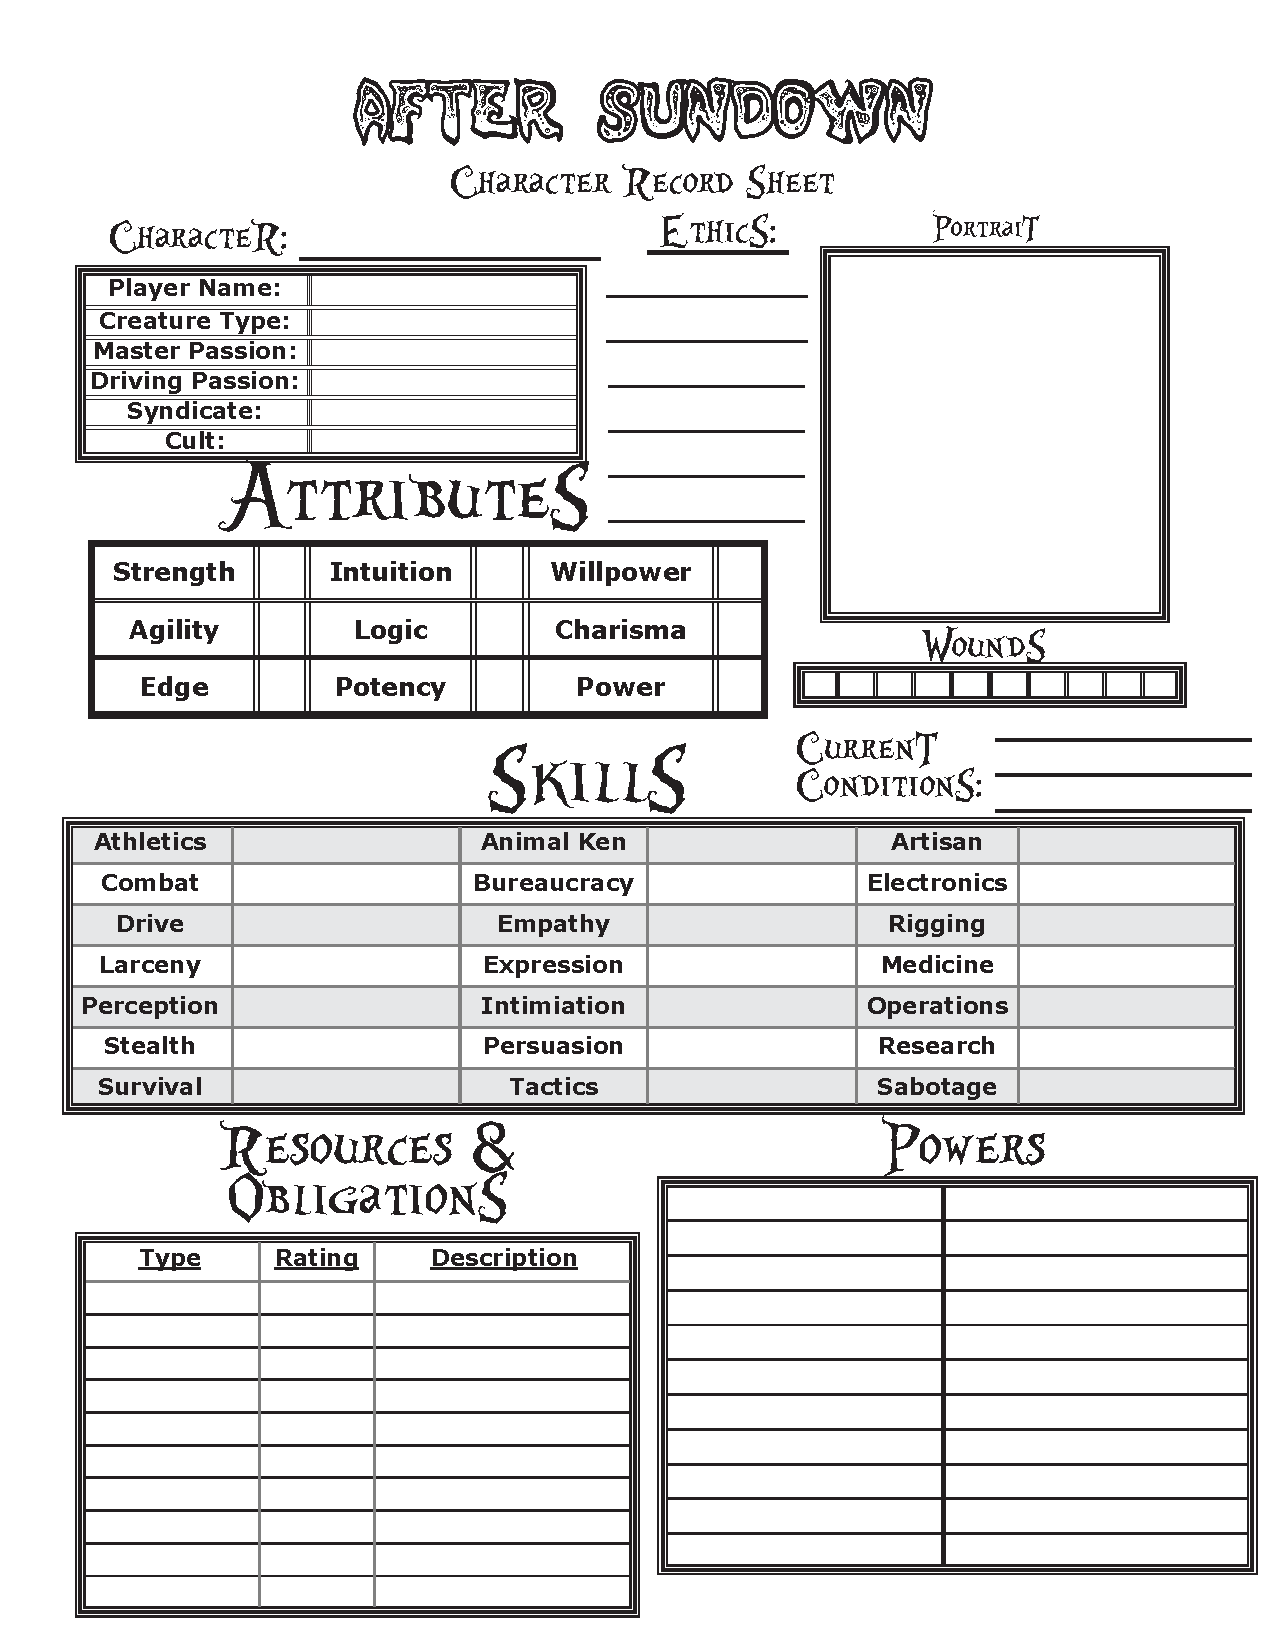
\includepdf[pages={1,2}]{images/Character-Sheet.pdf}

\end{document}